\documentclass[12pt]{article}
\usepackage[UTF8]{ctex} 
\usepackage[hidelinks]{hyperref}
\usepackage{listings}

\usepackage{graphicx}
\usepackage{float} 
\usepackage{subfigure}
\usepackage{amsmath} 
\usepackage{booktabs}
\usepackage{tcolorbox}

% 加宽目录编号区域，避免 100+ 编号与文字重叠
\makeatletter
\renewcommand*{\l@section}{\@dottedtocline{1}{1.5em}{3.2em}}
\renewcommand*{\l@subsection}{\@dottedtocline{2}{4.7em}{3.5em}}
\makeatother

% 图片计数
\usepackage{chngcntr}
\counterwithin{figure}{section}
\renewcommand{\thesubfigure}{\arabic{subfigure}}

\lstset{
   % language=Python, % 设置语言
 basicstyle=\ttfamily, % 设置字体族
 breaklines=true, % 自动换行
 keywordstyle=\bfseries\color{NavyBlue}, % 设置关键字为粗体，颜色为 NavyBlue
 morekeywords={}, % 设置更多的关键字，用逗号分隔
 emph={self}, % 指定强调词，如果有多个，用逗号隔开
    emphstyle=\bfseries\color{Rhodamine}, % 强调词样式设置
    commentstyle=\itshape\color{black!50!white}, % 设置注释样式，斜体，浅灰色
    stringstyle=\bfseries\color{PineGreen!90!black}, % 设置字符串样式
    columns=flexible,
    numbers=left, % 显示行号在左边
    numbersep=2em, % 设置行号的具体位置
    numberstyle=\footnotesize, % 缩小行号
    frame=single, % 边框
    framesep=1em % 设置代码与边框的距离
}

\lstdefinestyle{mystyle}{basicstyle=\ttfamily, breaklines=true, keywordstyle=\bfseries, commentstyle=\itshape\color{black!50!white}, stringstyle=\bfseries, columns=flexible, numbers=left, numbersep=2em, numberstyle=\footnotesize, frame=single, framesep=1em}

\begin{document}

\tableofcontents
\newpage

\section{GPU Vs CPU}

从这两张图（图1.1）来看，左侧代表中央处理器（CPU），右侧代表图形处理器（GPU）。两者似乎都包含相似
的组件或单元。例如，两者都有动态随机存取存储器（DRAM）和不同级别的缓存。具体来说，GPU配备了两个缓存级别，其功能与
CPU中的缓存类似；而CPU包含三个缓存级别——L1、L2和L3。接下来来看算术逻辑单元（ALU）。

这个单元负责执行应用程序的指令。CPU中只有数量有限的ALU，而GPU则包含数百甚至数千个类似单元，称为核心（Core）。鉴
于以上相似性——两者都有全局内存、都有多级缓存——我们自然会问：它们之间到底有什么区别？


\begin{figure}
    \centering
    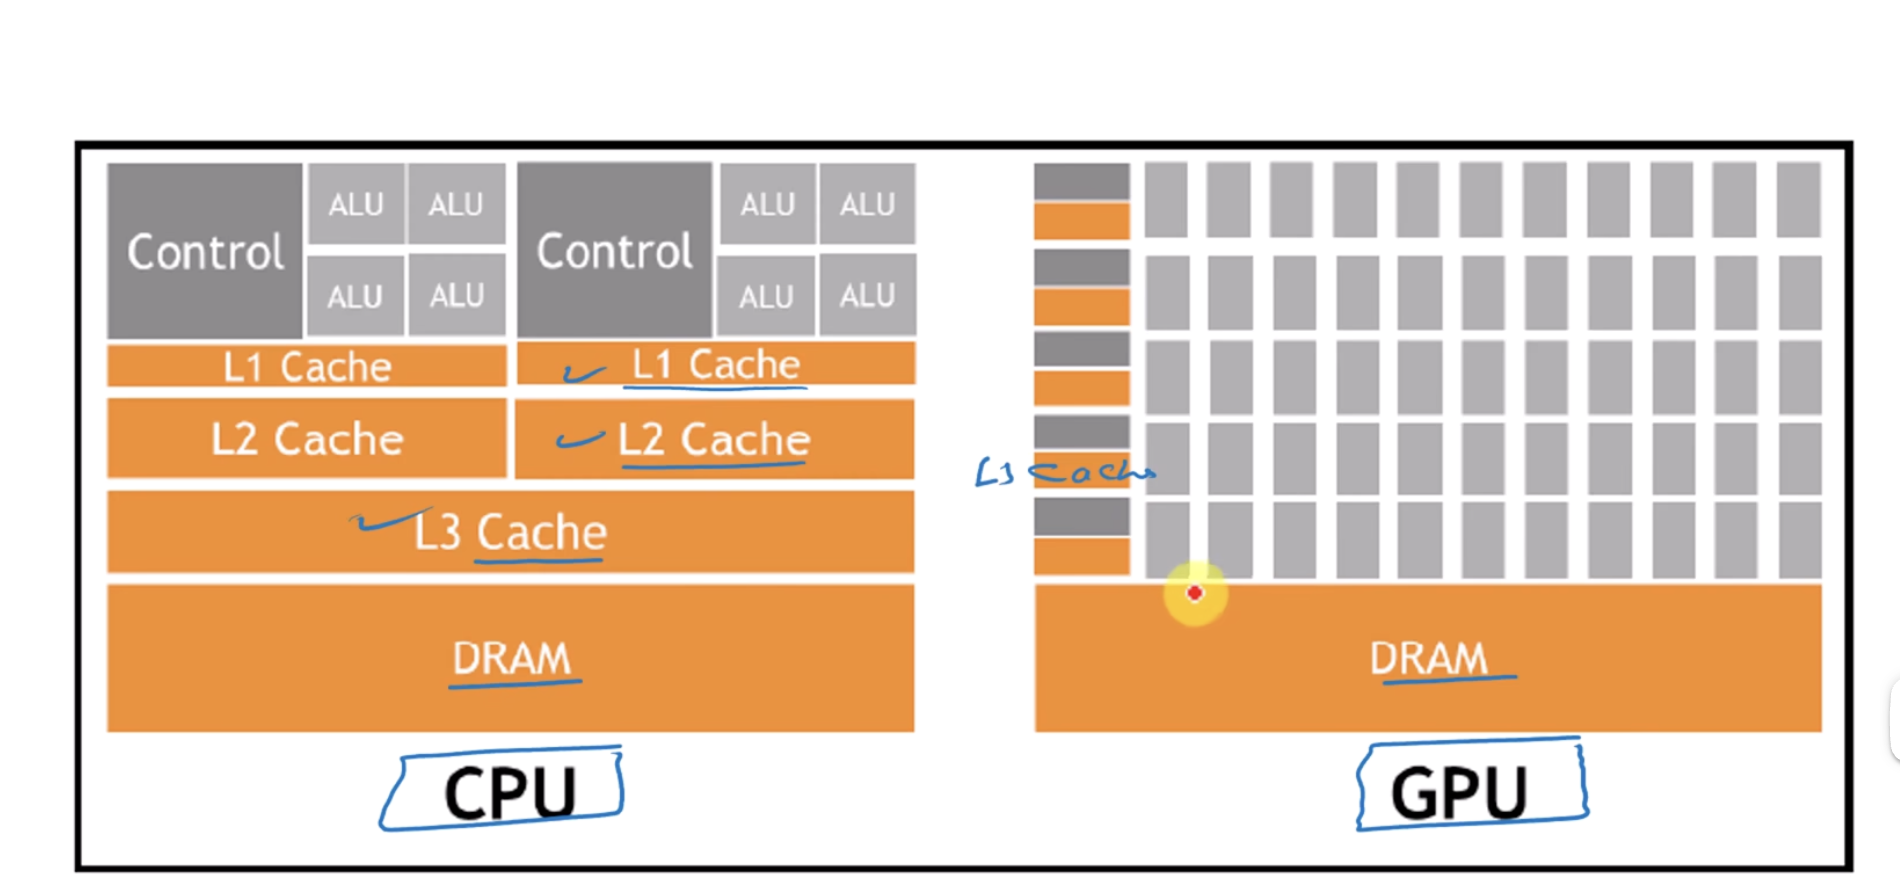
\includegraphics[width=0.8\linewidth]{resources/cuda-001.png}
    \caption{GPU Vs CPU}
    \label{fig:placeholder}
\end{figure}


\subsection{ALU与核心的对比}

CPU中有ALU，而GPU中有核心。为了理解它们的区别，以及为什么大多数系统同时需要CPU和GPU，让我们来仔细分析。在一对一
的比较中，CPU中的ALU明显比GPU中的核心更强大、更复杂。这里的"一对一"指将CPU中的一个ALU与GPU中的一个核心进行
单独对比。当我们说一个ALU"更强大"时，指的是速度等属性——例如现代CPU的运行频率可达3到4 GHz。而作为对比，一款
2020年发布的GPU——英伟达A100——其频率范围在765到1200 MHz之间。


需要明确的是，1200 MHz 意味着 1.2 GHz，大约只是主流 CPU 速度的四分之一。另一方面，GPU 核心更为专精，通常设计用于
高效执行特定类型的任务。CPU 中的 ALU 是为通用任务设计的，专注于快速执行单个线程。而 GPU 核心则是为并行性设计的——
它们经过优化，可以同时处理大量线程，这使它们非常适合像渲染图形这类需要对大量元素并行执行相同操作的任务。

理解 CPU 和 GPU 之间的这些区别非常重要，因为它们直接影响了应用程序的性能。毕竟本课程的核心目标，就是利用 GPU 和并行编
程来优化应用程序性能。那么，核心数量的差异具体如何影响性能呢？

\begin{figure}
    \centering
    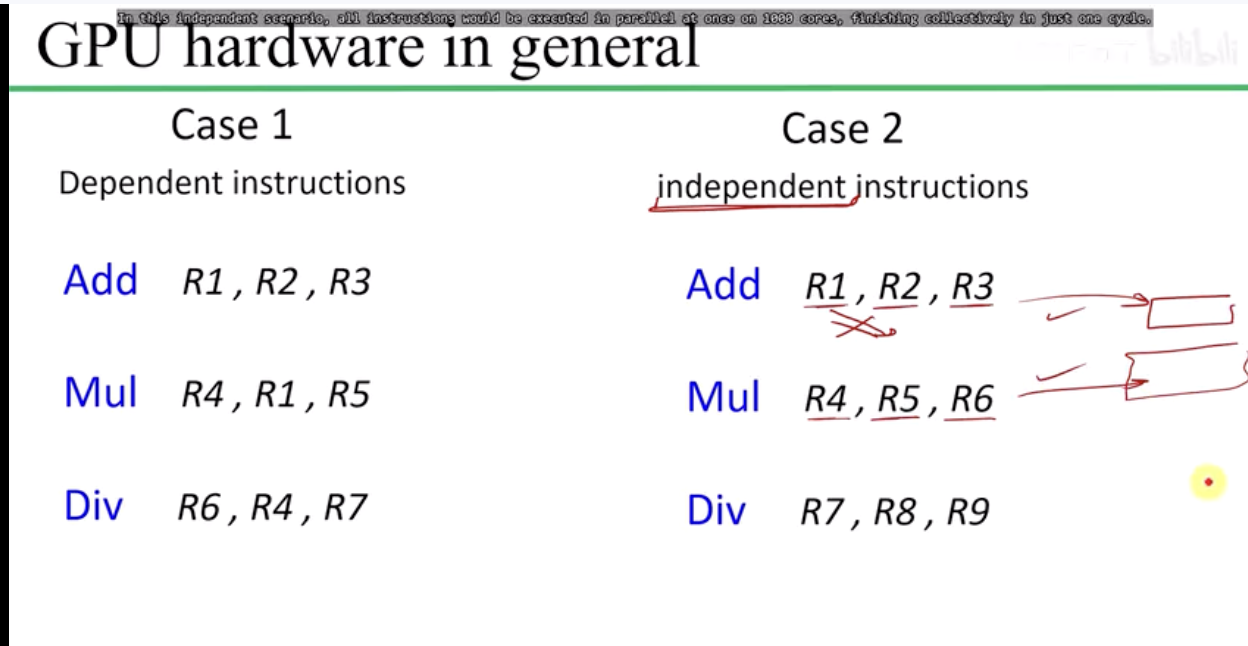
\includegraphics[width=0.75\linewidth]{resources/cuda-003.png}
    \caption{两种计算场景}
    \label{fig:placeholder}
\end{figure}

\subsection{顺序执行与并行执行}

我们将研究两种场景。在第一种场景中，假设大多数应用程序指令是相互依赖的——每条指令都依赖于前一条指令的结果。为此，我们
来看三条指令，每条执行不同的操作：第一条将两个值相加，第二条将它们相乘，最后一条进行除法运算。具体来说，第一条指令从
寄存器 R2 和 R3 中取值相加，并将结果存储在 R1 中。

接着将 R1 中的值与 R5 相乘，将结果存储到 R4 中。这里的关键是这些指令之间的相互依赖性：第二条指令使用了 R1，这个寄存器
正是前一条加法指令的目标寄存器。这意味着在执行乘法之前，加法操作必须先完成。

第二条指令依赖于第一条的结果。同样，除法操作必须等待乘法操作的结果，因为它涉及 R4，而乘法结果就存储在那里。这种处理方式
被称为顺序执行——指令以串行方式一条接一条地执行。你可能会想：为什么不利用多个核心来并行执行这些指令，一步完成呢？在这个
例子中，我们需要三步来执行这三条指令。即使有三个独立的核心分别处理加法、乘法和除法，它们也无法同时运行——第二条指令仍需
等待第一条，第三条等待第二条。

这引出了一个问题：在这种场景下，CPU中少量的ALU反而是理想的选择。如果CPU最适合此类任务，那么我们何时需要GPU？答
案在于指令的性质。虽然我们讨论的场景最适合CPU，但GPU在应用程序内指令相互独立的情况下表现得最为出色。为了说明这一点，
我们来看另一个例子——这次使用相同的加法、乘法和除法指令，但改为每条指令相互独立。

指令之间是独立的，因此如果我们有多个可用核心，就可以将每条指令分配给一个独立的核心，同时并行执行它们。这还可以大规模地发生
。在相互独立的情况下，1000条指令可以在1000个核心上并行执行，总共只需一个周期即可完成。例如，假设我们有1000条指令，
每条执行只需一个周期。而在相互依赖的情况下，将需要1000个周期，因为每条指令必须等待前一条指令完成。

从以上讨论中我们可以推断出：CPU 是专门为顺序操作设计的；而当处理充满大量独立指令的任务时，GPU则处于领先地位——因为
它们能够跨多个核心同时运行多条指令。这里的"顺序"指的是每条指令都依赖于前一条指令的结果。

\subsection{硬件架构}

有一种常见的误解是 GPU 在所有情况下都比 CPU 更好，但这并非事实。接下来我们看看 CPU 和 GPU 在大多数系统中是如何共存的
。下图展示了大多数电脑中的通用主板。你可以看到 CPU 插槽旁装有风扇，专门用于保持 CPU 冷却、防止过热。

主板上还有 DRAM 插槽、电源接口，以及关键的外围组件互连（PCIe）接口。将 GPU 插入 PCIe 插槽后，它就通过主板总线与
CPU 建立了直接连接。PCIe 接口至关重要，因为它允许连接多种扩展卡，包括 GPU、网卡和声卡。当我们把 GPU 插入 PCIe 插槽
时，它就与 CPU 连接起来了。下图展示了 CPU 与 GPU 之间的这种典型连接方式。


\begin{figure}
    \centering
    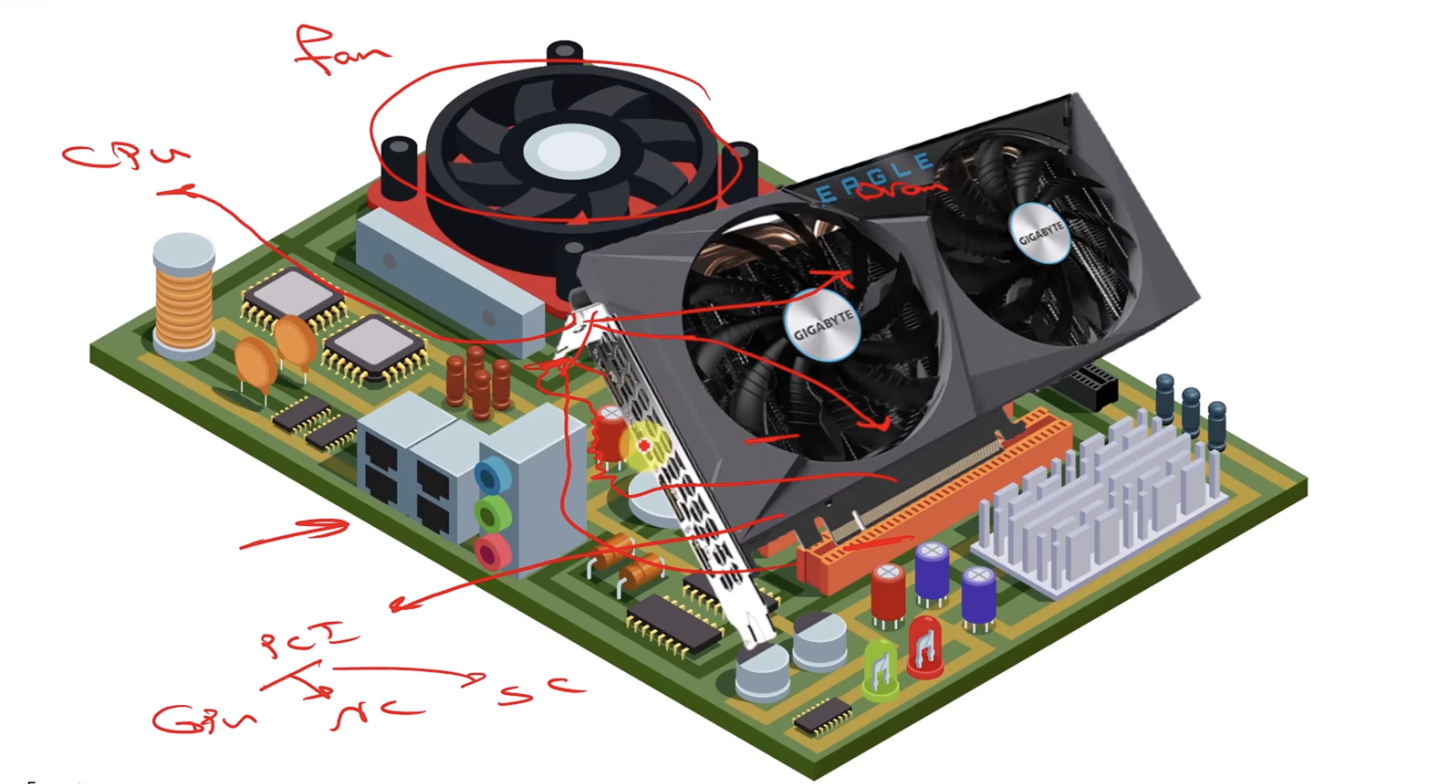
\includegraphics[width=0.75\linewidth]{resources/cuda-002.png}
    \caption{硬件架构}
    \label{fig:placeholder}
\end{figure}

同样，GPU 也有其专用的全局内存。回顾上图，CPU 的全局内存（DRAM）位于内存插槽中，通过总线直接连接到 CPU。

而 GPU 的全局内存则集成在 GPU 扩展卡本身的电路板上。图中绿色方框代表的就是 GPU 扩展卡。本课程的目标正是从最基础的知识
开始，清晰地讲解每一个部分。

\subsection{GPU内部组件}

现在让我们深入分析 GPU 中的关键组件，特别聚焦于英伟达的 GPU。在 GPU 内部有一个关键单元，称为流多处理器（Streaming 
Multiprocessor，简称 SM）。这个术语在本课程中将频繁出现，因此从一开始认识到它的重要性至关重要。此外，诸如调度器和分发
器等组件也存在，我们将在后续章节中更深入地探讨。

除了流多处理器之外，GPU 中还存在多种内存级别，例如 L2 缓存和全局内存。深入来看，每个流多处理器配备了多种针对特定任务
设计的核心：其中一些核心专门用于执行浮点运算，另一些则执行整数运算。

\begin{figure}
    \centering
    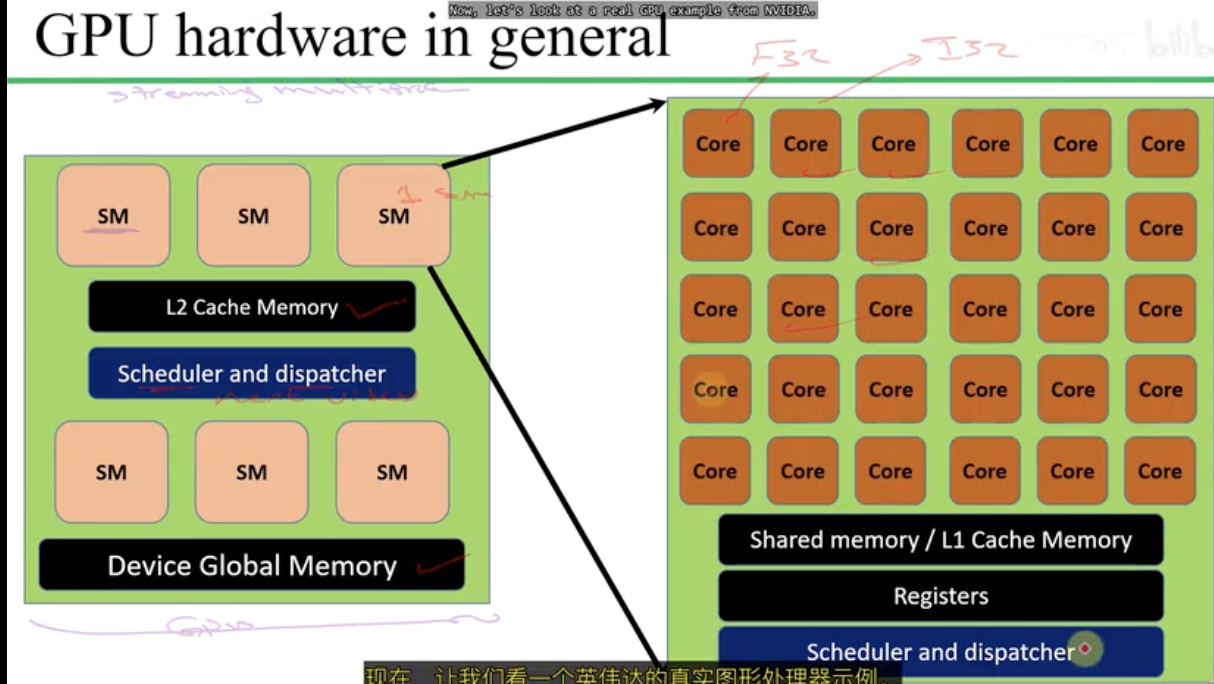
\includegraphics[width=0.75\linewidth]{resources/cuda-004.png}
    \caption{GPU 架构}
    \label{fig:placeholder}
\end{figure}

\subsection{A100 GPU实例}

让我们以英伟达 A100 GPU 为例来看一个真实 GPU 及其流多处理器。A100 于 2020 年发布。下图展示了单个流多处理器的一部分（
并非整个 SM，更不是整个 GPU）。在 SM 内部有 L1 缓存，而 L2 缓存则位于整个 GPU 内部（SM 外部）。需要记住的关键点是
：L1 缓存位于 SM 内部，而 L2 缓存是更广泛的 GPU 层级的组成部分。

\begin{figure}
    \centering
    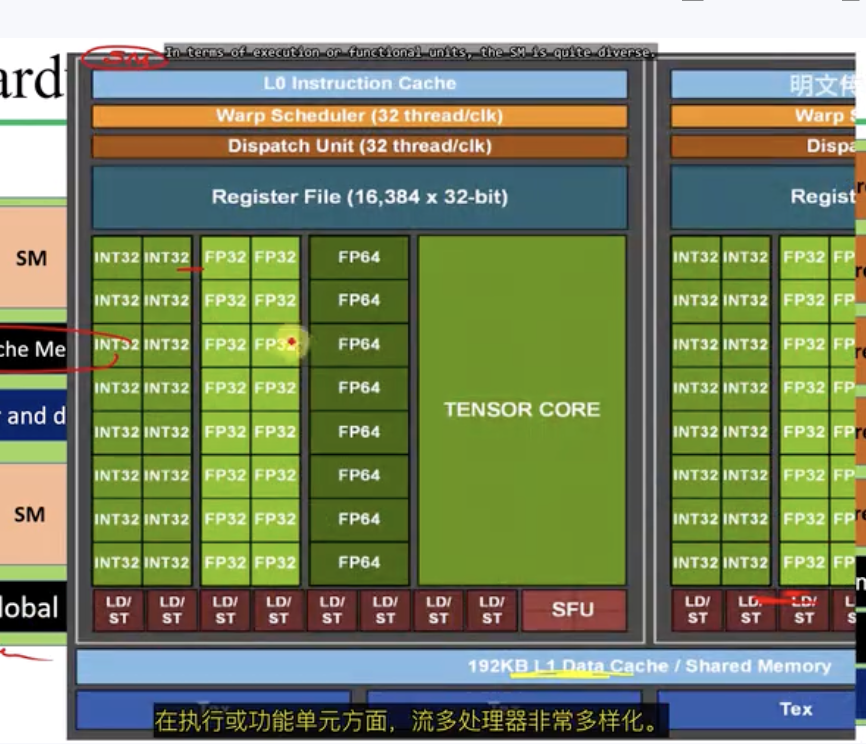
\includegraphics[width=0.75\linewidth]{resources/cuda-005.png}
    \caption{A100 GPU 架构}
    \label{fig:placeholder}
\end{figure}

在执行或功能单元方面，流多处理器非常多样化。我们发现了专门为矩阵乘法操作设计的张量核心（Tensor Core）、用于处理浮点运算
的浮点核心，以及整数核心。此外，如前所述，SM 包含一个调度器单元、一个分发器单元和若干个寄存器。当涉及内存交互时，SM 配
备了加载/存储单元和一些特殊功能单元（SFU）——这些单元负责从内存中读取以及向内存写入数据，并处理诸如对数计算等特定任务。

这张详细的图片仅展示了 GPU 架构白皮书中一个 SM 四分之一部分的快照——这里指的是整个 GPU 的结构图，而非单个 SM。这张
特定的图片详细展示了英伟达 A100 GPU 的规格。在接下来的章节中，我们将更深入地探讨白皮书是什么、在哪里可以访问它们，以
及其他相关细节。

\begin{figure}
    \centering
    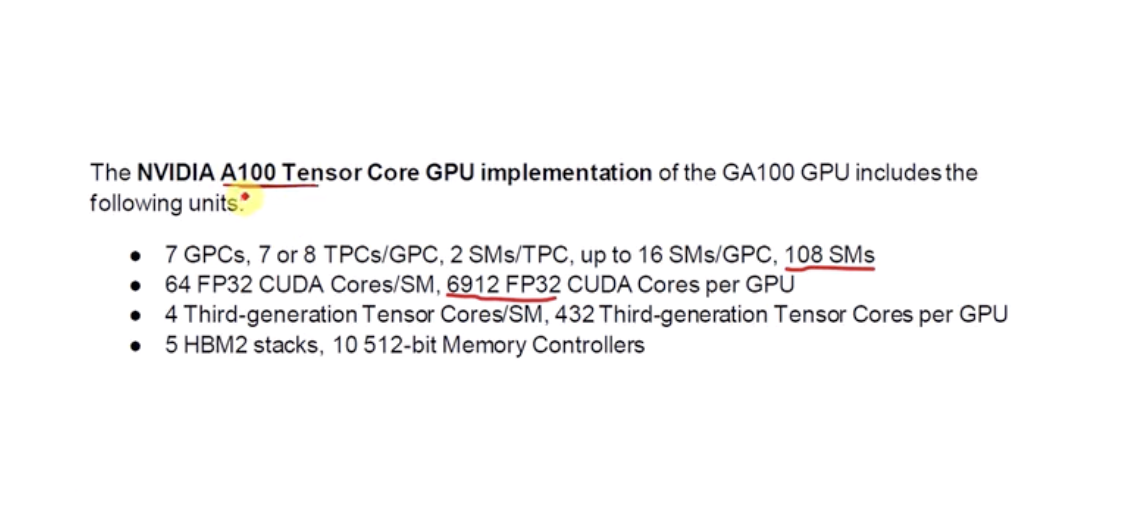
\includegraphics[width=0.75\linewidth]{resources/cuda-006.png}
    \caption{A100 特性}
    \label{fig:placeholder}
\end{figure}


每个 SM 包含 64 个单精度核心。在 A100 GPU 内部，约有 108 个 SM，这意味着整个 A100 GPU 拥有约 7000 个单精度核心——
这是一个非常大的数量。该 GPU 还拥有另外 7000 个专用于整数运算的核心。此外，深入研究 A100 的内部结构，你还会发现特殊功
能单元（SFU）以及张量核心。正是这些核心凭借其庞大的数量所提供的巨大计算能力，使 A100 GPU 成为全球众多高性能超级计算机
的核心组件。例如，META 公司宣布了他们雄心勃勃的计划——建造世界上最强大的超级计算机。如果你查阅 META 官方网站的文章，就会清楚地
看到他们的超级计算机架构严重依赖于 A100 GPU。

在最近的发展中，有推测称他们可能会整合 2022 年发布的新款 H100 GPU——这是在 A100（基于 Ampere 架构）发布两年后推出
的。与 A100 相比，H100 拥有进一步的进步和增强，我们将在本课程中讨论这两者。

你可以在 TOP500 网站
\href{https://top500.org/lists/top500/2023/06/}{https://top500.org} 上找到超级计算机排名列表。
为了强调英伟达 GPU——特别是 A100 GPU——的重要性，让我们看看全球前 500 名超级计算机。该网站提供了关于世界领先超级计
算机的详细信息。从数据中可以看到，A100 GPU 存在于前十名超级计算机中的三台里：它被集成到排名第四的莱昂纳多（Leonardo）超
级计算机中，以及排名第八和第九的超级计算机中。

感谢你与我们一同深入 GPU 的世界，我们下章再见。


\section{NVIDIA 历史}

在上个世纪的最后二十年里，几家如今众所周知的巨头公司相继成立，其中最伟大之一就是英伟达（NVIDIA）。英伟达由黄仁勋于
1993 年创立。成立仅两年后，英伟达推出了其第一款产品——NV1。该设备设计相当简单，其 GPU 仅有 2 MB 内存、64 位总线
宽度和单个核心。要了解如今的差距，可以将其与最新的 GPU GeForce RTX 4090 Ti 进行比较：RTX 4090 Ti 拥有约 18,000
个核心，而 NV1 只有 1 个核心。


\begin{figure}
    \centering
    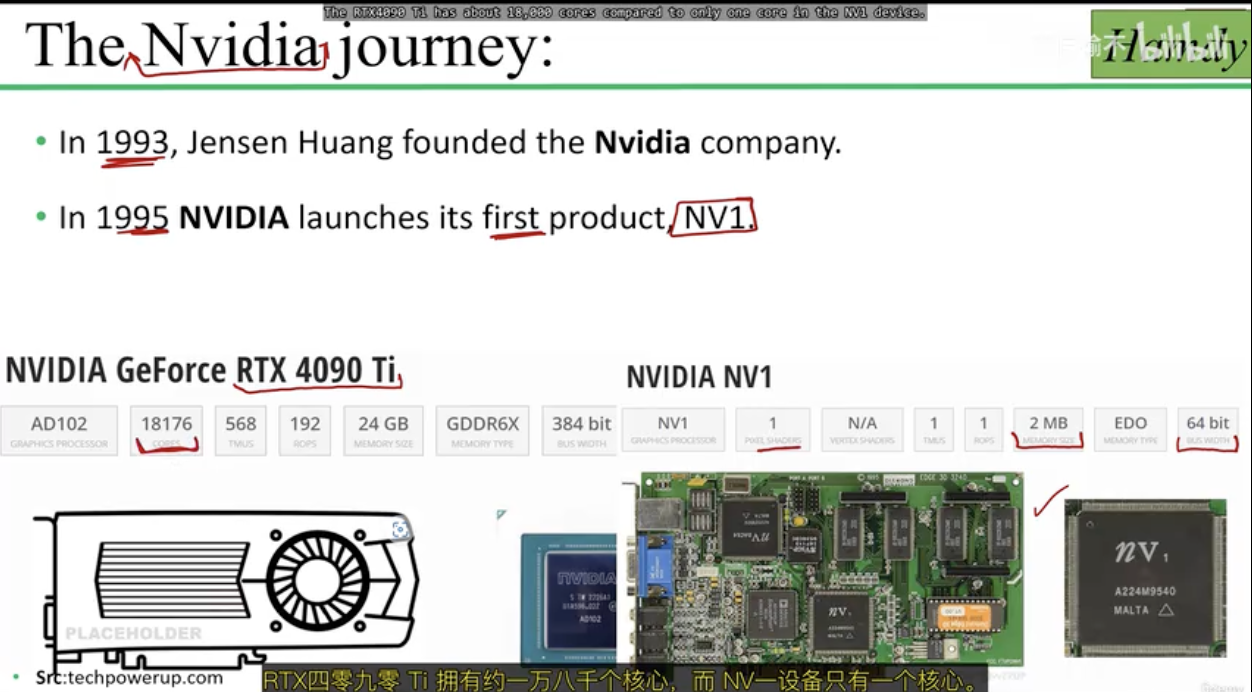
\includegraphics[width=0.75\linewidth]{resources/cuda-007.png}
    \caption{NVIDIA 历史}
    \label{fig:placeholder}
\end{figure}

核心数量方面，增长了约 18,000 倍。而内存容量从 NV1 的 2 MB 增加到 RTX 4090 Ti 的 48 GB，增长约 24,000 倍。此
外，再看看对应用程序性能至关重要的运行频率——已从 75 MHz 大幅提升至约 2400 MHz，带来 32 倍的速度提升。这充分展示了
GPU 技术在过去 25 年间的巨大演变。

\subsection{RIVA 128}

暂时放下这些数据，我们继续往下看。1997 年，英伟达推出了 RIVA 128，也称为 NV3。该型号是首批为消费级市场带来三维加速的
GPU 之一，这也是为什么它比其前身 NV1 更成功。值得注意的是，RIVA 128 是英伟达首次取得重大市场成功的产品，在巩固其市场
地位方面发挥了关键作用——四个月内销量即达到约 100 万台。

\begin{figure}
    \centering
    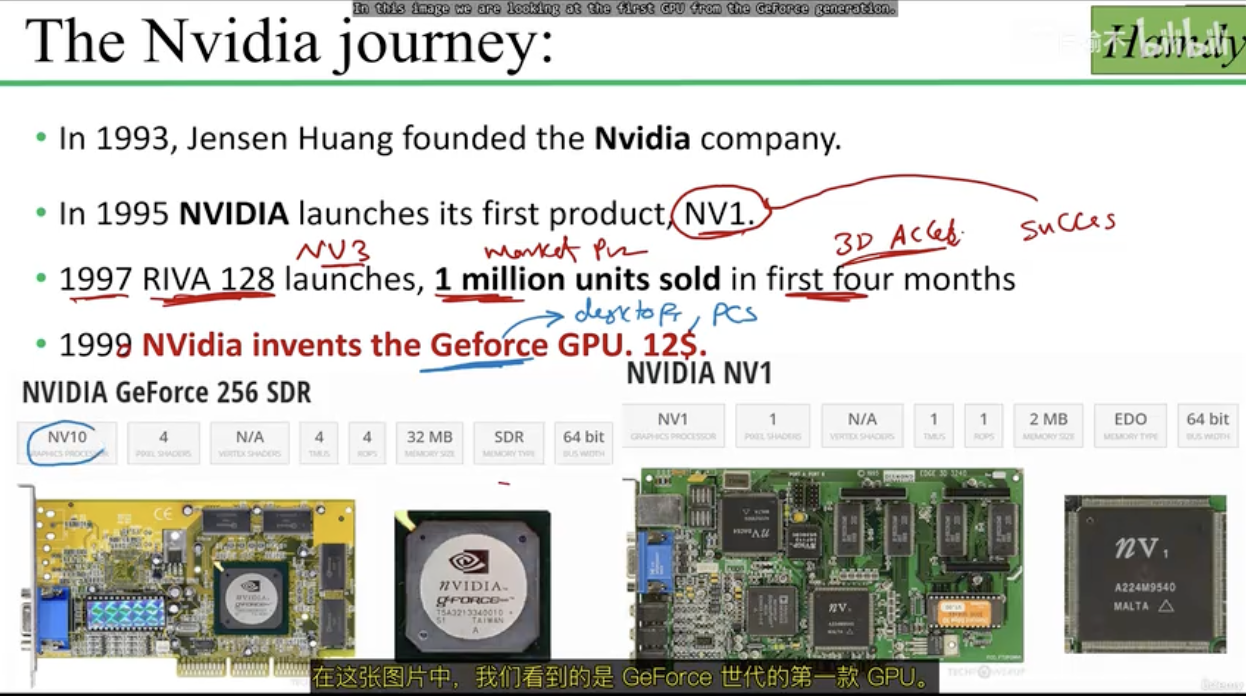
\includegraphics[width=0.75\linewidth]{resources/cuda-008.png}
    \caption{GeForce}
    \label{fig:placeholder}
\end{figure}

\subsection{GeForce世代}

GeForce 这一品牌为许多人所熟悉，因为这些 GPU 在问世一两年后就广泛出现在台式机和笔记本电脑中。具体来说，1998 年英伟达
揭开了后来成为其标志性 GPU 世代的 GeForce 系列的序幕。此次发布标志着 GPU 技术领域的一次革命性转变。从图中可以看到，
GeForce 系列的首款 GPU 与 NV1 相比差异巨大——它拥有四个核心，相对于英伟达第一款 GPU NV1 的单核心来说是一个巨大的飞
跃。别忘了，那是在 1998 年，一台设备中有四个核心本身就是一场革命。内存容量也从 NV1 的 2 MB 增加到 32 MB，增长了 16 倍。

从那时起，英伟达就成为全球 GPU 领域最知名的公司。如今，英伟达既是推动计算加速的关键力量，也主导着游戏产业。以上便是英伟
达发展历程的简要概述。


\section{GPU架构与代系关系}

\subsection{架构的定义}

在英伟达 GPU 的语境中，有两个关键概念需要解释：世代与架构。先说架构——它指的是 GPU 的基本设计和结构，涵盖了 GPU 在最
基础层面的构建方式：核心的排列与管理、数据处理和传输的技术，以及渲染图形和计算任务的方法。每种新架构通常都会在处理能力、
能效以及对新功能的支持方面带来改进，例如光线追踪或 AI 驱动的任务。

英伟达的 GPU 架构决定了 GPU 的性能与能力。英伟达为每种架构赋予不同的代号，通常使用著名科学家或发明家的名字，如 Turing
和 Pascal。例如，Turing 架构引入了实时光线追踪以及用于 AI 计算的核心单元。而在 Pascal 架构中，我们可以看到对其前身的一
些改进，例如更多的核心和更高的时钟频率。总而言之，GPU 架构至关重要，因为它为 GPU 的能力奠定了基础，影响着从游戏图形到
科学计算的方方面面。

下图展示了英伟达的若干 GPU 架构，可以看到英伟达每 1 到 2 年就会发布一个新架构。在后续章节中，我将带你了解从 Fermi 架构开
始的各个英伟达架构。

\begin{figure}
    \centering
    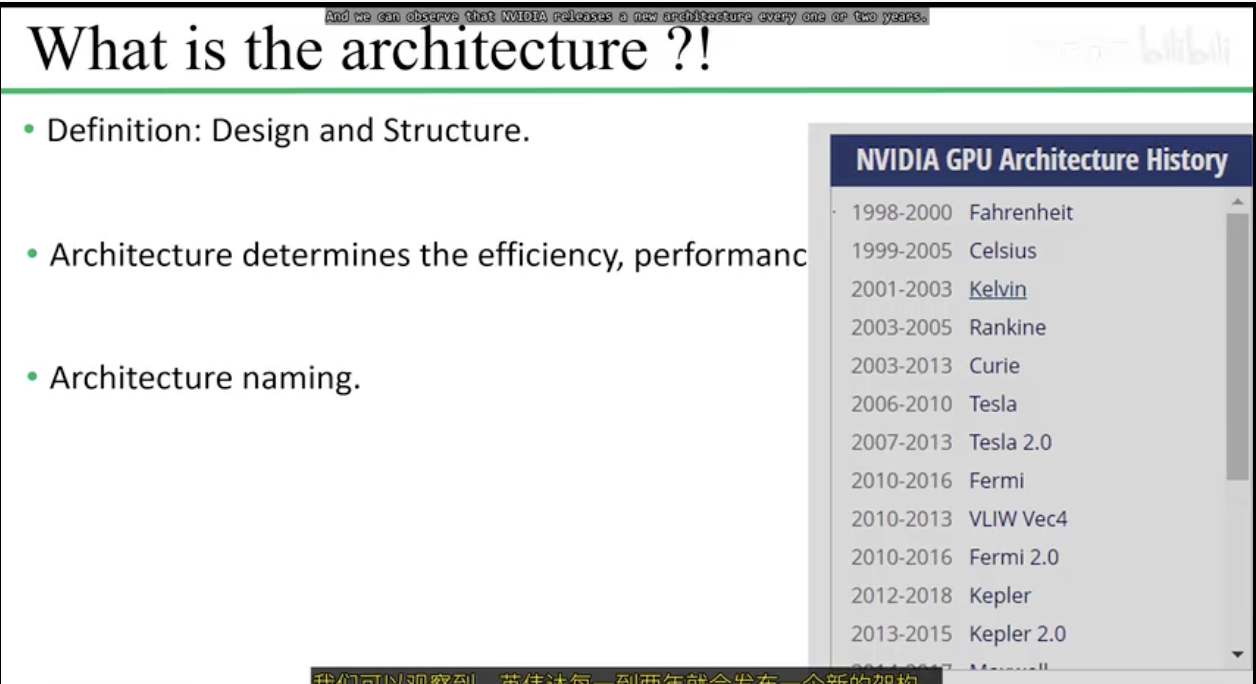
\includegraphics[width=0.75\linewidth]{resources/cuda-009.png}
    \caption{GPU架构}
    \label{fig:placeholder}
\end{figure}

接下来谈谈英伟达的不同世代。英伟达将其产品分为两个不同的类别：第一类面向普通消费者，涵盖我们在笔记本电脑、台式机和工作站
中使用的 GPU；第二类服务于高性能计算（HPC）领域，这在云计算等场景中至关重要。META、亚马逊、微软和谷歌都是 HPC 提供
商的典型代表。

第一类别包括 Tegra、GeForce 和 Quadro 等世代系列，其中 GeForce 和 Quadro 也是游戏 GPU 的热门选择——我想大多数人都
熟悉它们，因为它们常见于许多笔记本电脑中。

而第二类别（HPC 类别）中有一个世代被称为 Tesla。需要指出的是，这个 Tesla 与埃隆·马斯克的公司没有任何关联——它只是为高
性能计算设计的一系列 GPU 的统称。

\begin{figure}
    \centering
    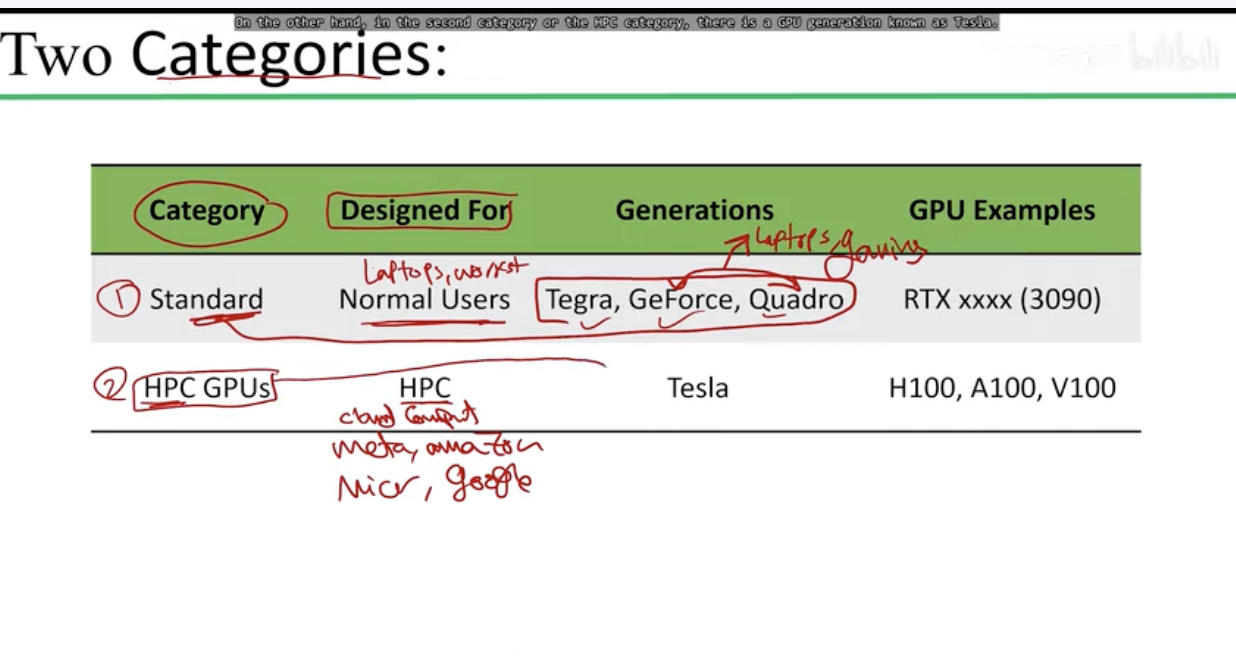
\includegraphics[width=0.75\linewidth]{resources/cuda-010.png}
    \caption{GPU架构}
    \label{fig:placeholder}
\end{figure}


\subsection{架构与世代的关系}

下表旨在总结这两个术语之间的区别：世代指的是 GPU 的具体用途，例如是用于 HPC 服务器还是标准台式机。而架构，如前所述，
指的是 GPU 芯片的设计与能力。每个架构可能包含多个不同的世代。在世代一栏，我们看到了 Tegra、GeForce、Quadro 和 Tesla 
这些名称；而 Hopper、Ampere 和 Volta 则是英伟达提供的不同架构。

\begin{figure}
    \centering
    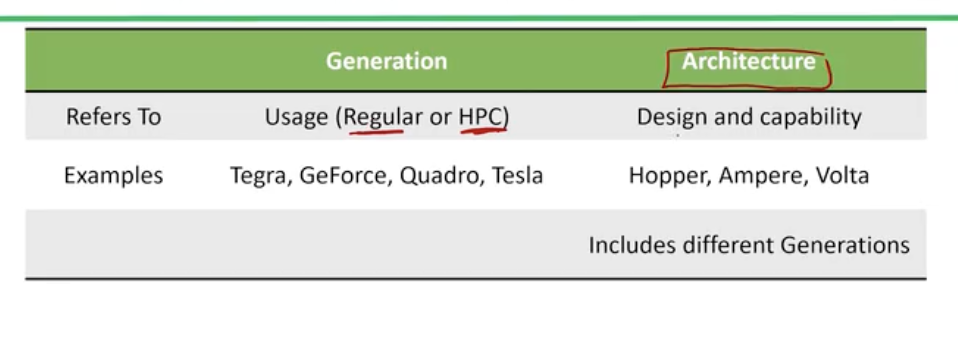
\includegraphics[width=0.75\linewidth]{resources/cuda-011.png}
    \caption{GPU架构}
    \label{fig:placeholder}
\end{figure}


为了说明这一点，考虑一下 2020 年发布的 Ampere 架构。这个架构包含了多个世代的 GPU。例如，在 Ampere 架构内，你既可以
找到 GeForce 世代的 RTX 3090，也可以找到 Tesla 世代的 A100——这两款 GPU 基于相同的 Ampere 架构芯片，但面向的应用截
然不同：RTX 3090 属于 GeForce 系列，主要设计用于游戏等消费级用途；而 A100 属于 Tesla 世代，专为超级计算机和云服务器等
HPC 环境设计。

\begin{figure}
    \centering
    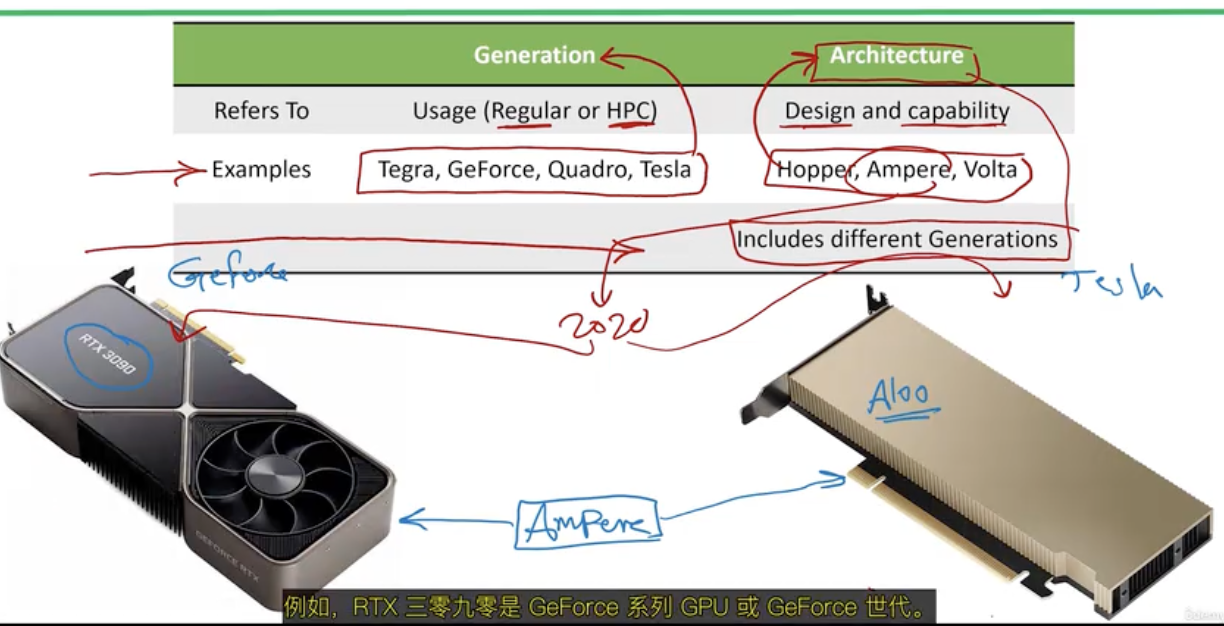
\includegraphics[width=0.75\linewidth]{resources/cuda-012.png}
    \caption{GPU架构}
    \label{fig:placeholder}
\end{figure}


总之，我们可以这样理解：每当英伟达整合了新的软件或硬件增强功能，就会宣布一个新架构；然后基于这个新架构，再为普通消费者和
HPC 领域分别开发不同世代的 GPU。

\subsection{GPU世代分类}

现在让我们深入探讨不同类型的世代。下表展示了英伟达最知名的 GPU 世代之间的区别：Tegra、GeForce、Quadro 和 Tesla。

首先来看 Tegra。Tegra 是英伟达为智能手机、平板电脑和移动互联网设备等移动平台开发的片上系统（SoC），将 GPU 和 CPU 集成
在单一芯片中。第一款使用 Tegra 的产品是微软的 Zune HD 媒体播放器，于 2009 年 9 月发布。2017 年 3 月 15 日，Tech 
Insights 披露了任天堂 Switch，它同样由 Tegra 芯片驱动。

\begin{figure}
    \centering
    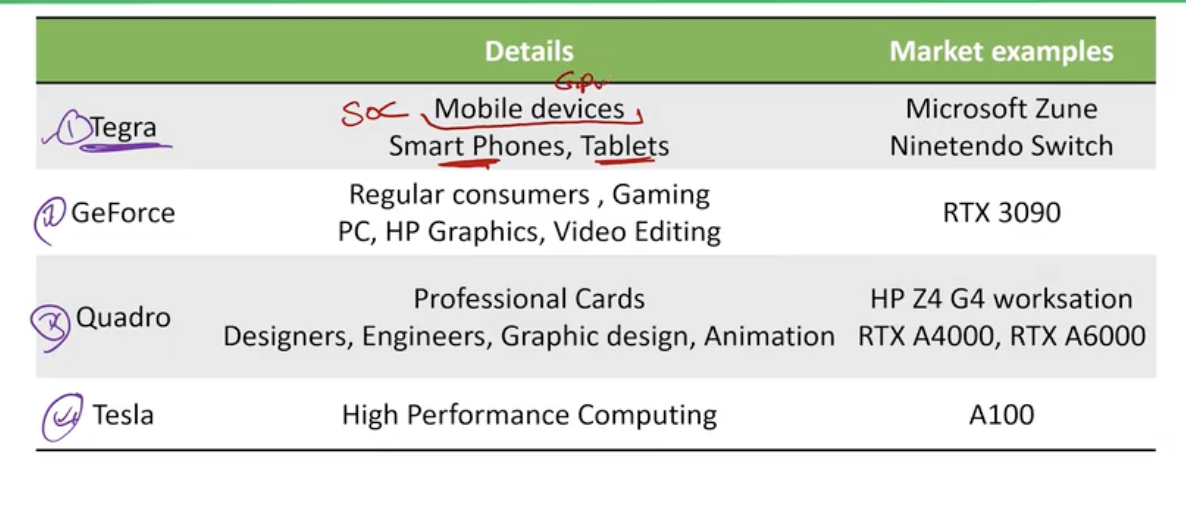
\includegraphics[width=0.75\linewidth]{resources/cuda-013.png}
    \caption{GPU架构}
    \label{fig:placeholder}
\end{figure}


接下来是 GeForce GPU——请注意，这一世代的 GPU 专为个人计算机打造，面向消费级市场，尤其是游戏玩家。这里说的是三维图形渲染
和游戏中的高性能，而非 HPC 级别的计算。它们也被普通消费者用于视频编辑和其他图形密集型任务。GeForce 系列中一个突出的例
子是 RTX 系列，如 GeForce RTX 3090、3080、3070 和 3060，这些是当前市场上该世代最知名的 GPU。接下来是 Quadro GPU——专业工作站显卡，专为需要高精度和计算能力的设计师和工程师打造。Quadro GPU 经过优化，适用于高级图
形设计、视频编辑和动画等专业软件。它在许多笔记本电脑中广泛使用，以提供增强的性能。此外，最新工作站（如 HP Z 系列）通常
也使用 Quadro GPU。

在离开 Quadro GPU 这个话题之前，让我们花点时间讨论一些最近的更新。例如 HP 最近推出的一款工作站——HP Z4 G4，这款工
作站可以配备高端的英伟达 Quadro RTX 显卡。但在未来的 GPU 中，我们将不再看到 Quadro 品牌。正如下图所示（来源见链接所
示），Quadro 命名已被 RTX 标签取代，我们只会看到 RTX 标签。

此外，同一网页包含一个表格，展示了各种 Quadro 系列与其对应英伟达架构之间的关系，以及它们在 RTX 系列中的新命名等价物。
表格的排列方式为：第一列列出了不同的 Quadro 系列，如 8000 和 6000 等。以 6000 系列为例，这一行展示了不同架构下的命名惯
例——在 Maxwell 架构中前缀是 M，在 Pascal 架构中前缀是 P，命名惯例为 Quadro 后跟系列数字（如 6000），前面加上架构的首字母。

\begin{figure}
    \centering
    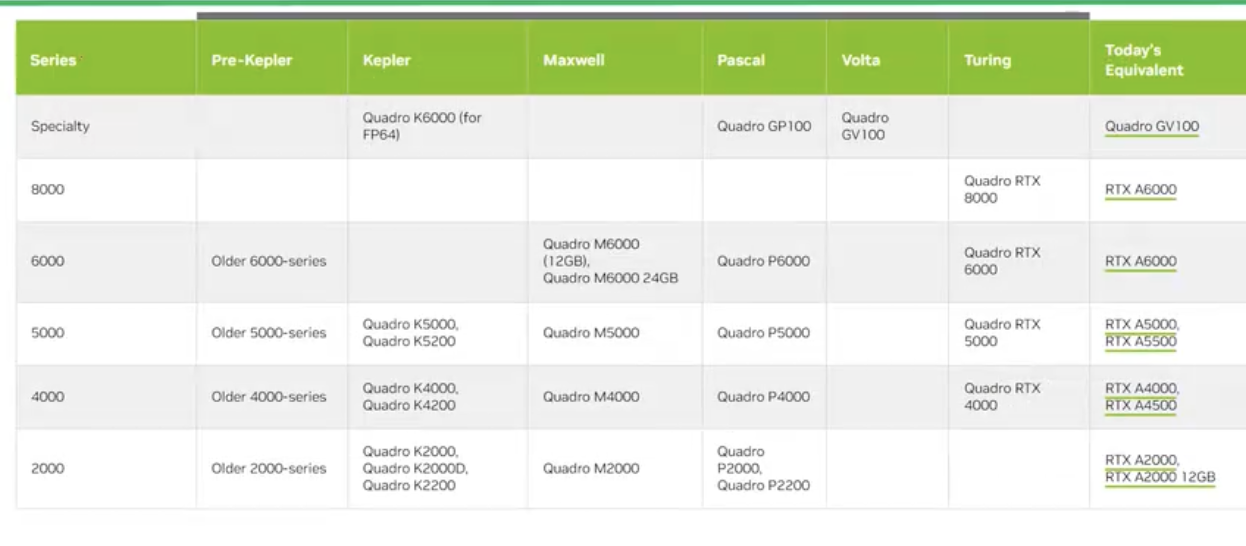
\includegraphics[width=0.75\linewidth]{resources/cuda-014.png}
    \caption{GPU架构}
    \label{fig:placeholder}
\end{figure}


在 Pascal 中前缀是 P。但在 Turing 架构中，RTX 标签被插入在 Quadro 和系列数字之间。正如我们所见，如果你打算在并行编
程或 GPU 领域工作，了解 GPU 的命名规则非常重要。然而，从 Ampere 架构开始，英伟达已经弃用了 Quadro 品牌，只使用 RTX 
前缀。

还有一点需要注意：在弃用 Quadro 术语之前，英伟达将 RTX 名称同时用于 Quadro 和 GeForce 两条产品线。例如 RTX 30XX 系
列，包括 RTX 3090、3080、3070 和 3060 等型号，都属于面向消费者（尤其是游戏玩家）的 GeForce 家族。

在专业领域（如设计和内容创作），正如表格所描绘的，曾存在 Quadro RTX 这样的型号。我们有 GeForce RTX 和 Quadro RTX 两
个系列，例如 Quadro RTX 4000、Quadro RTX 5000 和 Quadro RTX 8000。RTX 标签同时出现在 GeForce 世代和 Quadro 世代
中。但需要记住的是，在未来的 GPU 中，我们将不再看到 Quadro 品牌，只会看到 RTX。虽然这些信息乍一看可能让人应接不暇，但
这完全正常——当你更深入地研究 GPU 行业并开始使用这些产品时，命名和术语会变得更加熟悉，也更容易理解。

总而言之，我们在最顶层有 GPU 架构，每个架构可用于生产不同的世代。


\subsection{GeForce与Tesla在超级计算机中的应用}

现在让我们来看两种来自不同世代的 GPU 的真实案例，每个世代针对不同的市场细分——从 GeForce 这样的普通消费级 GPU 到为 HPC
设计的 Tesla 系列。正是这种区别，使得在全球前 500 名超级计算机中看到 GeForce 系列的 GPU 相当罕见，因为它并非为超级计算
机设计，而是为普通台式机和工作站设计的。

让我们深入 TOP500 网站进一步探索。如下所示，这是当年六月发布的前 500 名超级计算机列表。如果我们搜索 A100、V100 和
P100 等 GPU——这些都属于 Tesla 世代——可以观察到许多超级计算机采用了它们，因为 Tesla 正是为超级计算机等用途设计的。我
们将在接下来的章节中详细而深入地讨论这些 GPU。

另一方面，如果我们搜索 RTX 系列，结果显示在排名靠前的超级计算机中没有此类应用。我想现在你已经清楚了 GeForce 与 Tesla 
世代之间的区别。理解所有这些区别对于为你的特定应用选择正确的 GPU 至关重要。我们将在接下来的章节中更深入地介绍 GeForce 
和 Tesla 等不同世代。


\section{如何识别GPU架构与代际}

\subsection{使用TechPowerUp查询规格}

下面我们以 RTX 3090 和 A100 GPU 为例，介绍如何快速获取这些规格参数。

方法很简单：推荐使用 TechPowerUp 网站（\href{https://www.techpowerup.com/gpu-specs/a100-pcie-80-gb.c3821}{A100 页面}），
它收录了各大厂商详尽的 GPU 数据库。你只需在搜索引擎中输入"A100 GPU TechPowerUp"并回车，点击搜索结果中的对应链接，
即可查看该显卡的完整规格与详细信息。

\begin{figure}
    \centering
    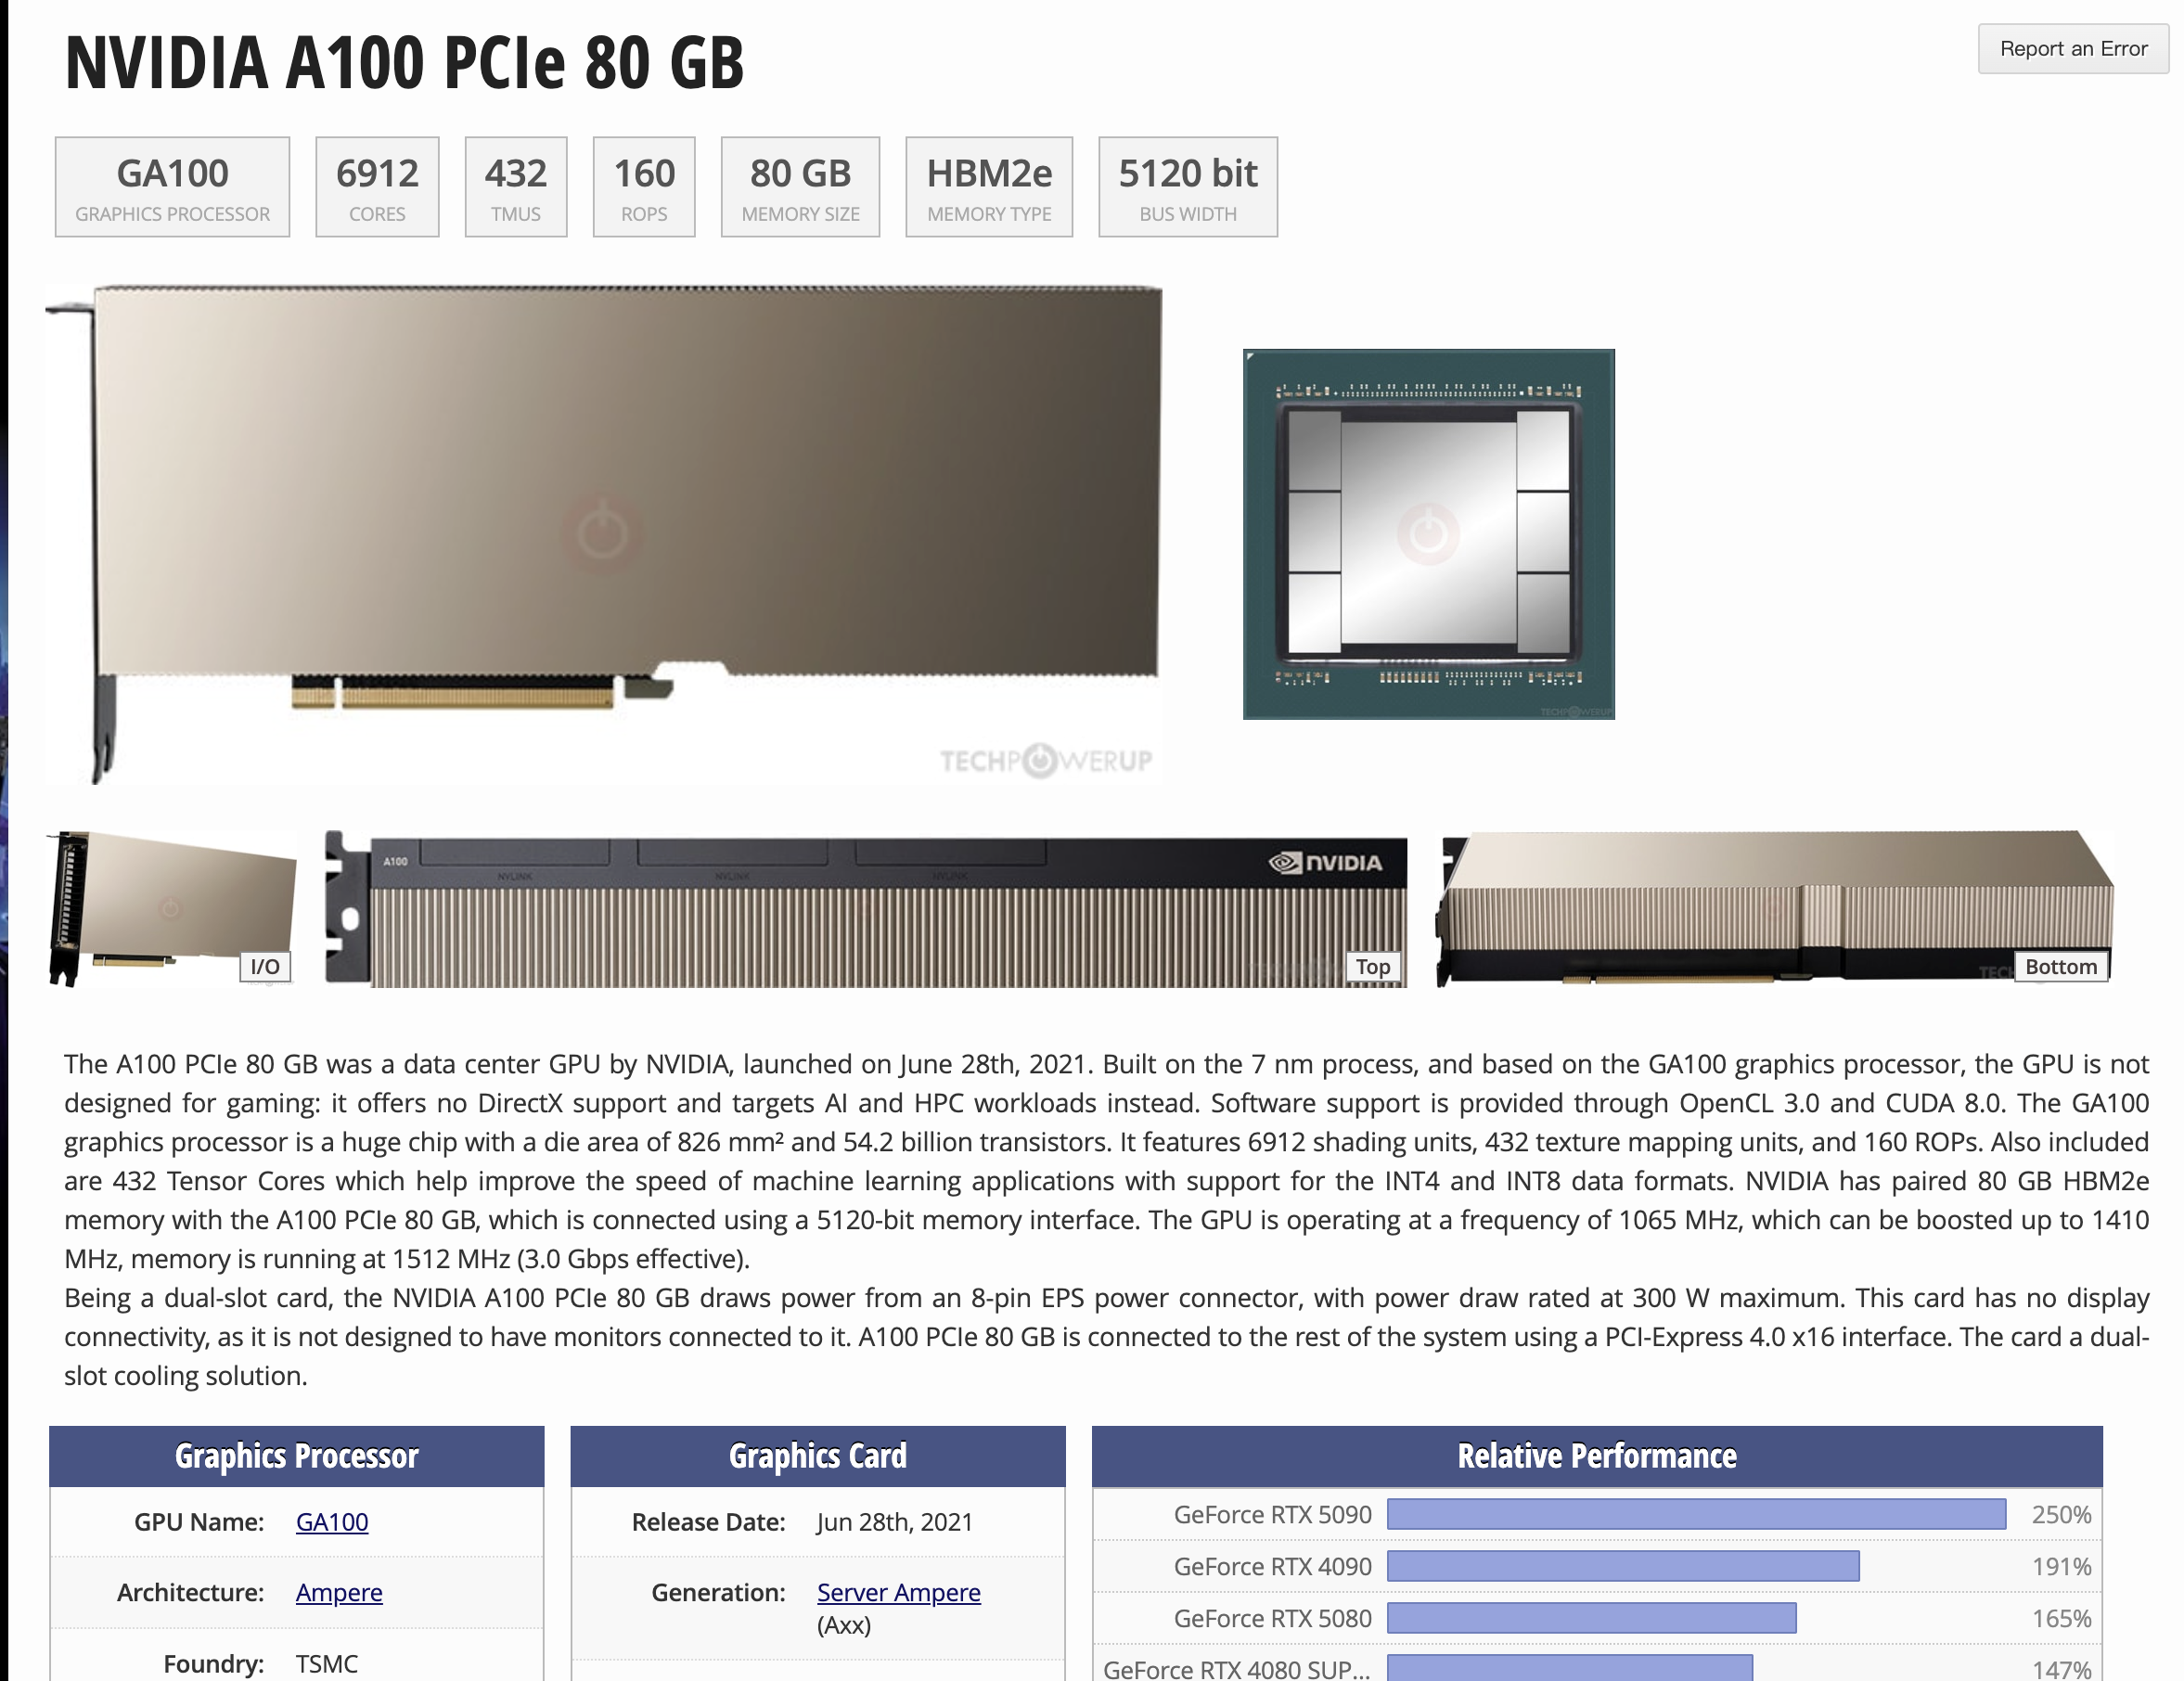
\includegraphics[width=0.75\linewidth]{resources/cuda-015.png}
    \caption{A100 GPU架构}
    \label{fig:placeholder}
\end{figure}

同样，你可以在 TechPowerUp（\href{https://www.techpowerup.com/gpu-specs/geforce-rtx-3090.c3622}{RTX 3090 页面}）
查 RTX 3090 的规格。现在对这两款 GPU 做一个简单的比较：首先是 GPU 芯片代号——A100 的代号为 GA100。关于 GPU 芯
片的具体含义我们将在后续章节中解释，这里只需关注它的名称。然后看核心数量：A100 拥有约 7000 个核心，而 RTX 3090 拥有
超过一万个核心。

\begin{figure}
    \centering
    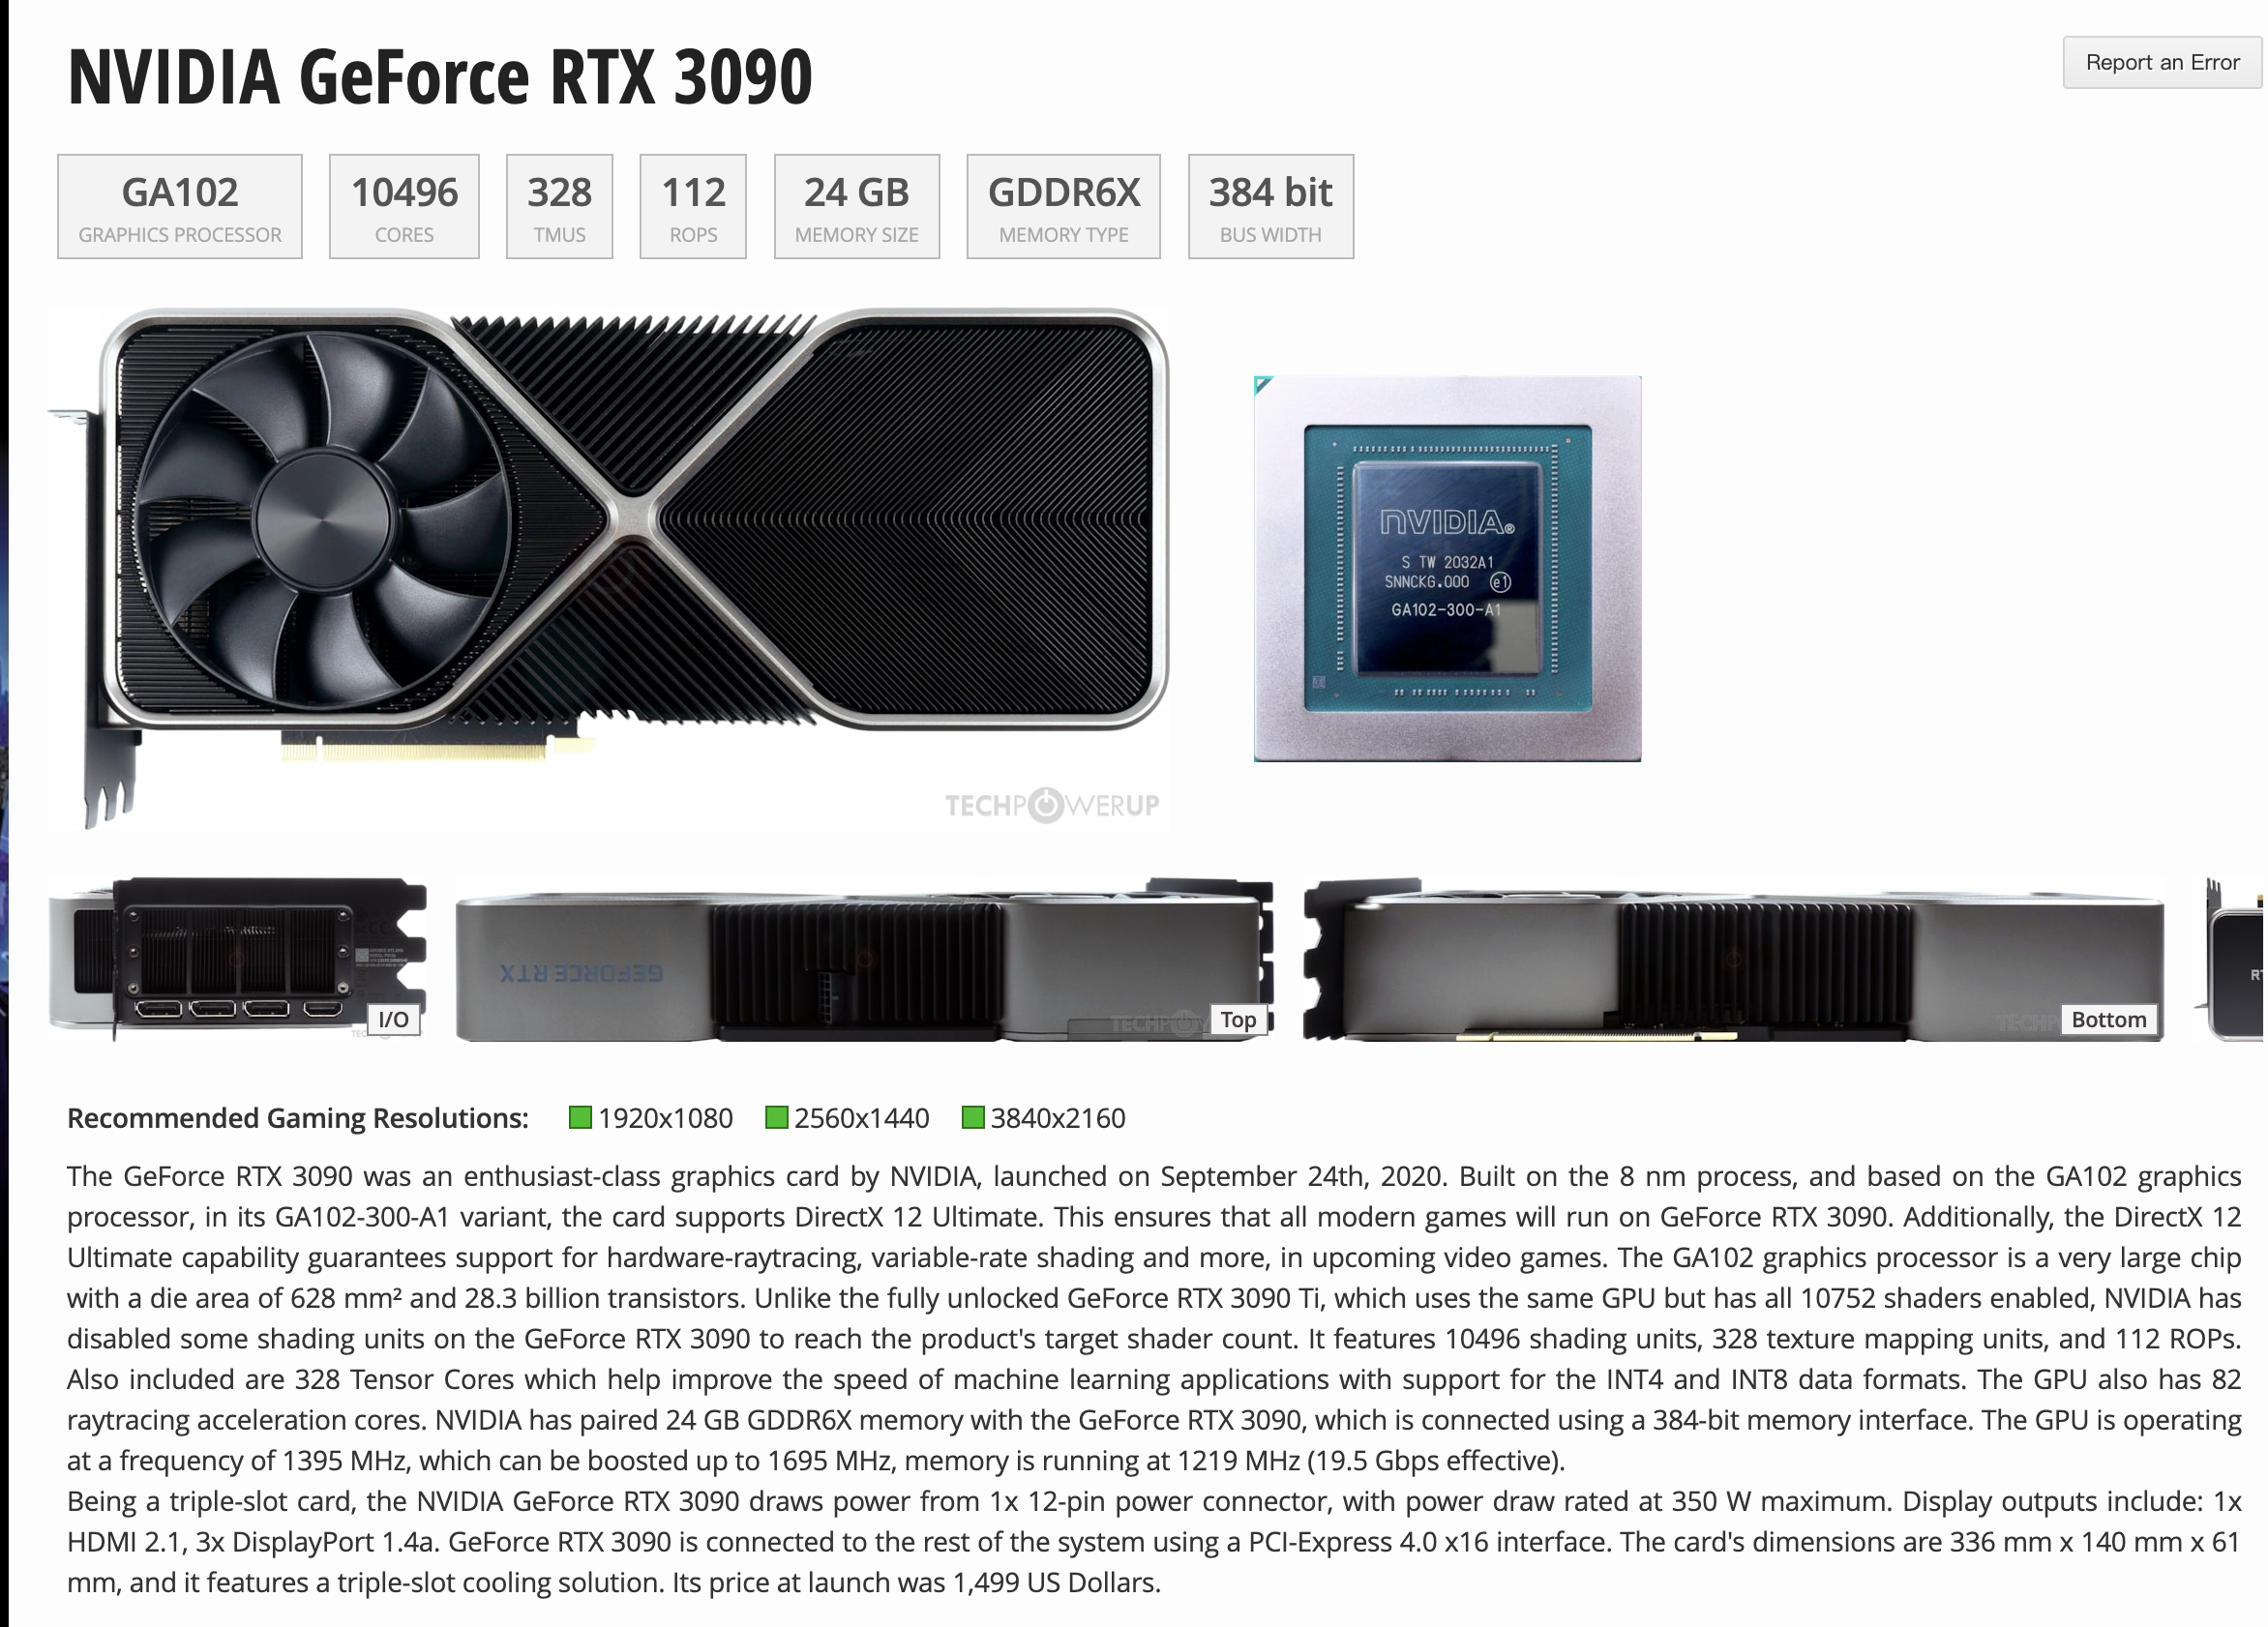
\includegraphics[width=0.75\linewidth]{resources/cuda-016.png}
    \caption{RTX 3090 GPU架构}
    \label{fig:placeholder}
\end{figure}

你在这里也可以看到许多规格参数，解释了每款 GPU 的不同能力。但本文先跳过这些，只关注世代和架构，后续章节将详细讨论更多
规格。不过请记住 6192 这个数字——这是专用于处理单精度运算的核心数量，并不代表用于各种操作的总核心数。举例来说，A100 
GPU 还包含用于处理整数运算和双精度运算的核心。这些将在后续章节中从官方白皮书和数据表中深入探讨，本文暂不展开。

\subsection{A100与RTX 3090架构对比}

现在让我们聚焦于这些 GPU 的世代和架构。以 RTX 3090 为例，其世代为 GeForce 30，架构为 Ampere。你还记得 GeForce 是
为谁设计的吗？正如上一章所述，它是为普通台式机、笔记本电脑和工作站设计的。

再来看 A100 GPU，其世代是 Tesla，正如前文所述，Tesla 世代专用于 HPC 服务器和超级计算机。值得关注的是，A100 与 RTX 
3090 共享相同的 Ampere 架构，尽管它们是为不同的应用场景而设计的。

这里引出一个重要问题：我们如何从外观上确认 GeForce 与 Tesla 世代之间的区别？


\subsection{视觉区分GeForce与Tesla}

检查这些 GPU 的图片时，你会注意到 Tesla GPU 通常没有板载冷却风扇。如果你看 A100 GPU 的图片，找不到任何冷却风扇。同样
，V100 GPU 也属于 Tesla 世代，搜索它的图片，可以看到它也不包含冷却风扇。其原因是这些 GPU 设计用于 HPC 环境，而这些环
境中配备了外部且更强大的冷却系统——如果你搜索全球任何超级计算中心的照片，就能看到其冷却系统的复杂性。

另一方面，GeForce GPU（例如我们电脑中的 RTX 系列）通常都配备内置风扇。这些风扇是标准台式机或工作站环境中散热所必需的
。这就是我们从外观上确认 GeForce 和 Tesla 世代之间区别的方法：Tesla GPU 无冷却风扇，GeForce GPU 有冷却风扇——原因就
在于它们所使用的目标环境不同。



\section{GPU 和 GPU 芯片}

\subsection{GPU芯片的定义}

本章我们将比较两个关键术语：GPU 和 GPU 芯片。本章非常重要，因为如果不理解 GPU 与 GPU 芯片之间的区别，就无法解释英伟
达生产的各种架构。

首先来说明这两个术语的区别，从 GPU 芯片开始。GPU 芯片代表着 GPU 的心脏——它是实际的硅核心，不附带任何外围组件。例如
，一款名为 GF100 的 GPU 芯片，其中的 F 指 Fermi 架构。在该芯片内部，集成了各种核心、内存控制器和其他负责 GPU 计算的电
子元件。而 GPU 则是消费者购买的最终产品，它集成了芯片以及必要的系统和接口，包括许多 GPU 中都存在的冷却机制。

\begin{figure}
    \centering
    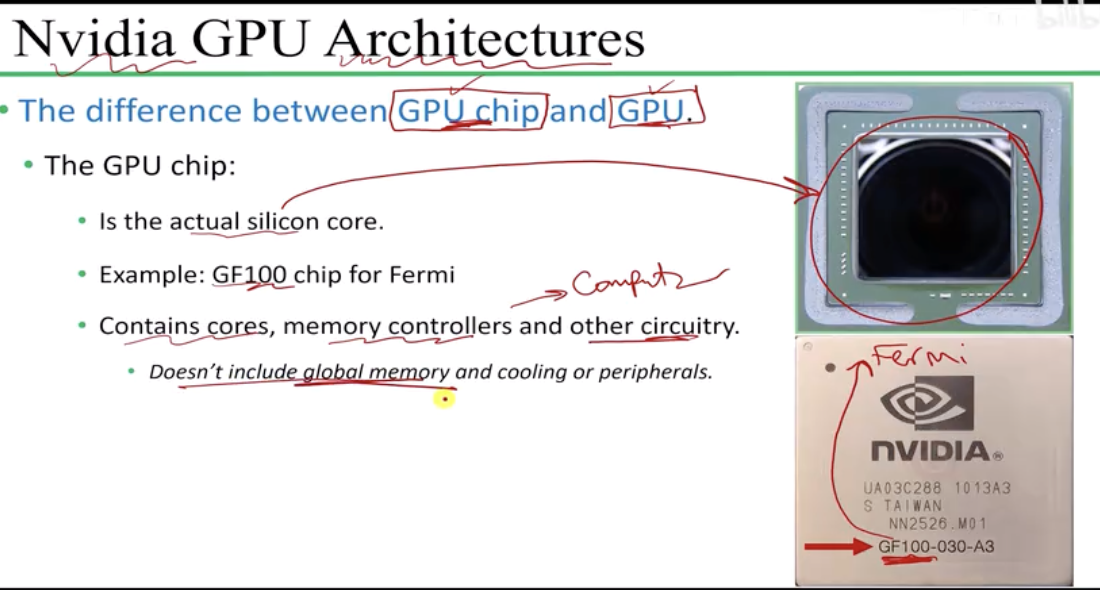
\includegraphics[width=0.75\linewidth]{resources/cuda-017.png}
    \caption{GPU 和 GPU 芯片}
    \label{fig:placeholder}
\end{figure}


\subsection{GeForce GTX 480与GF100芯片}

这款 GPU 由上文讨论过的 GF100 芯片驱动。下图展示的是 GeForce GTX 480 GPU——除了 GF100 芯片之外，它还包含全局内存单
元、显示端口（如 HDMI 端口）和一个冷却风扇。之所以需要冷却风扇，是因为它属于 GeForce 世代，这类环境需要风扇来散发计算
产生的热量。

\begin{figure}
    \centering
    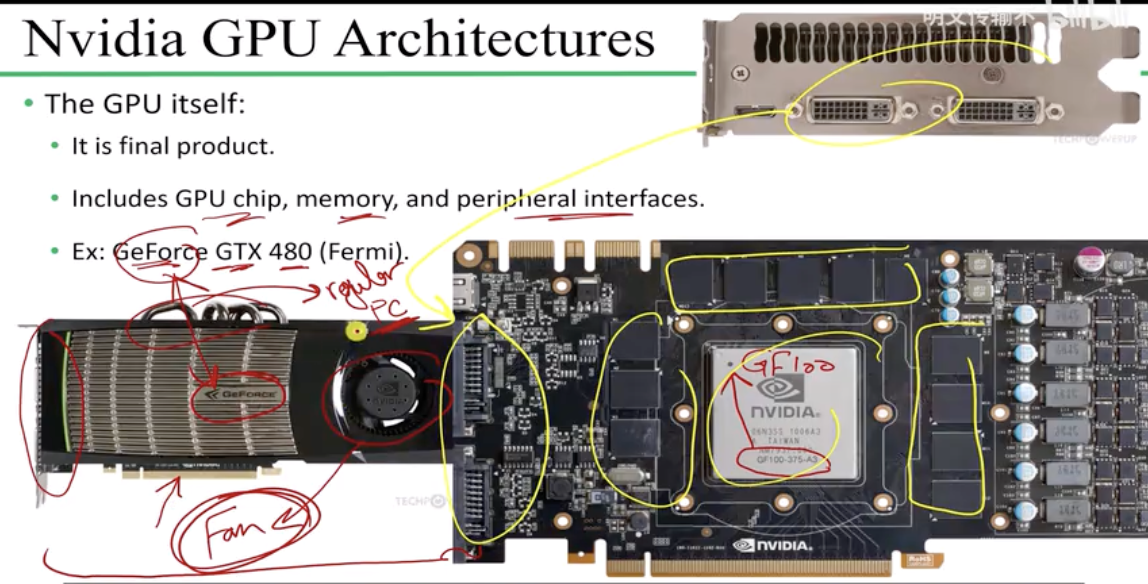
\includegraphics[width=0.75\linewidth]{resources/cuda-018.png}
    \caption{GPU 和 GPU 芯片}
    \label{fig:placeholder}
\end{figure}

根据之前的讨论，GeForce 世代是面向普通消费者的标准台式机和工作站设计的。

\subsection{A100与GA100芯片}

这两个术语之间区别的另一个例子可以从 A100 GPU 及其芯片中看到。基于 Ampere 架构的 A100 GPU，其名称中的字母 A 即体现
了这一点。与 Fermi 芯片类似的命名方式，驱动 A100 GPU 的芯片为 GA100。

\begin{figure}
    \centering
    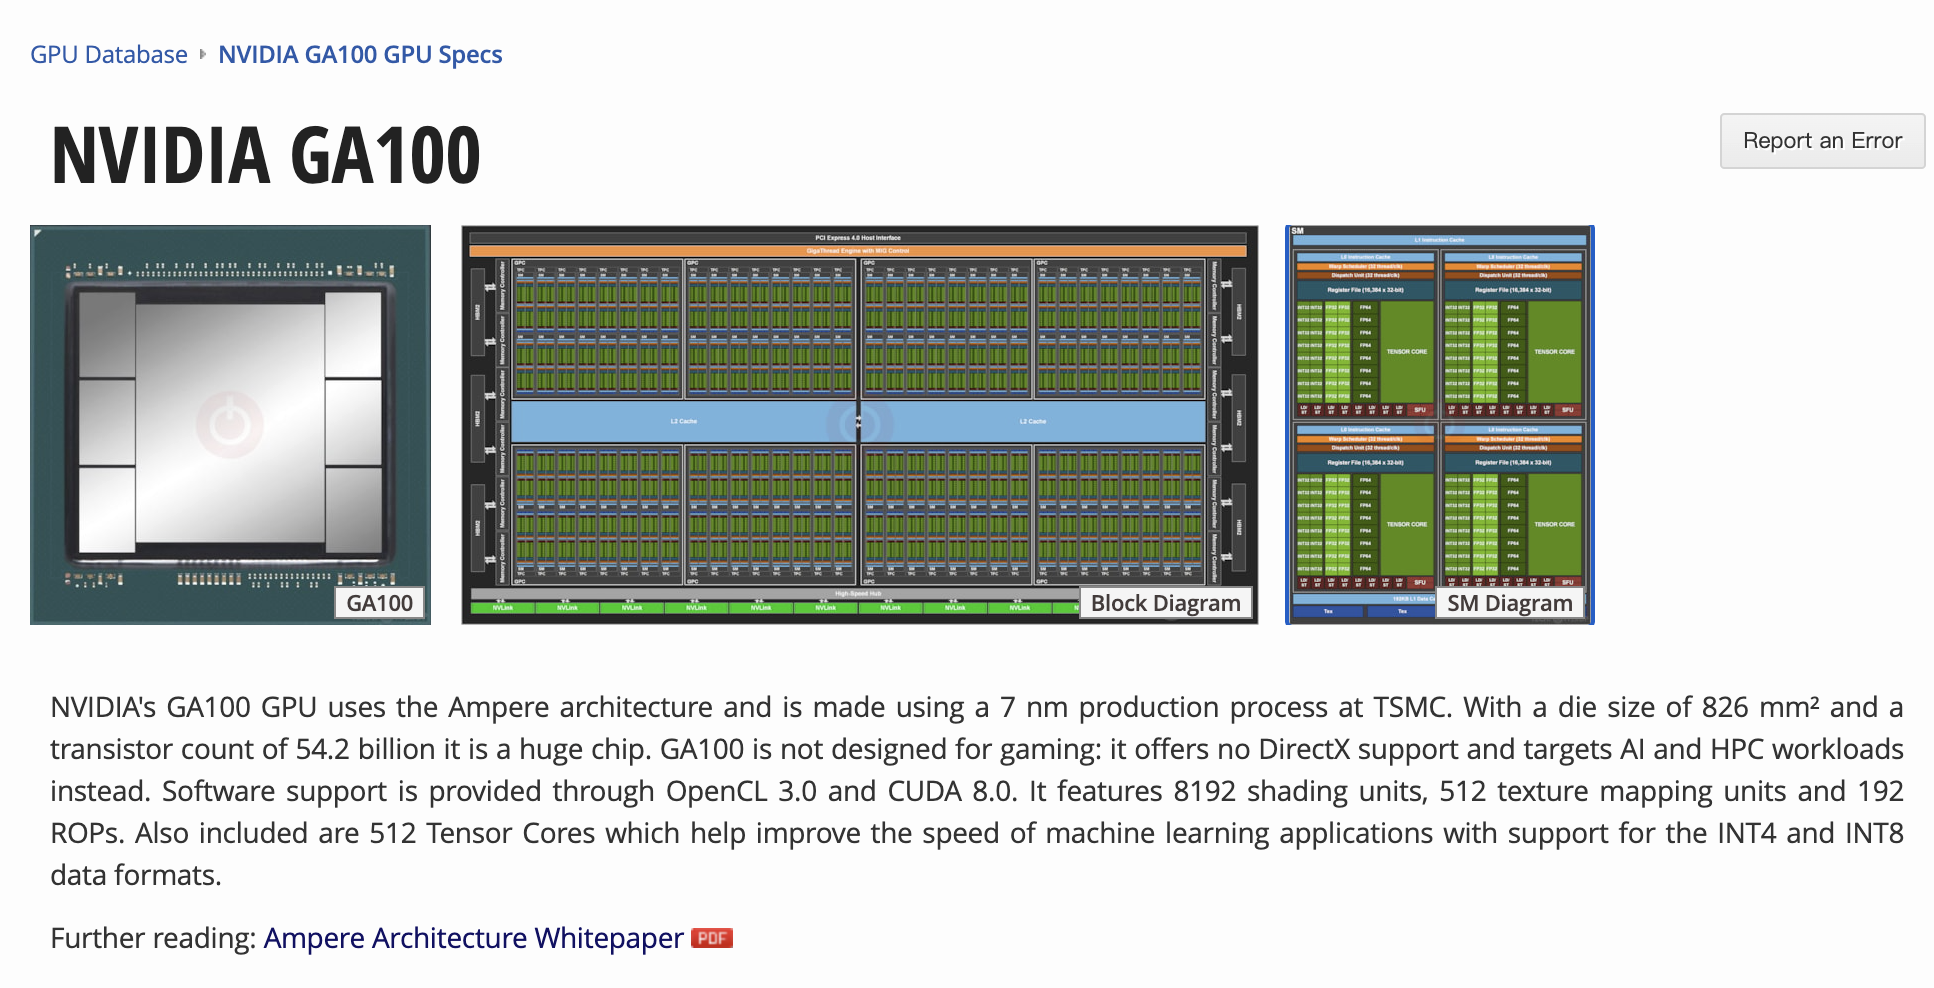
\includegraphics[width=0.75\linewidth]{resources/cuda-019.png}
    \caption{GA100芯片}
    \label{fig:placeholder}
\end{figure}

在 Fermi 架构中，芯片命名为 GF100。在 Ampere 架构中，芯片命名为 GA100。访问 TechPowerUp 网站，可以看到 A100 GPU 
的众多规格，网页上首先展示的就是芯片名称——GA100。通过搜索芯片名称 GA100，可以找到对应的链接，点击即可看到 GA100
芯片：如图所示，它仅是一块电子芯片，没有连接任何其他组件。

回到 A100 GPU 的网页，可以看到 A100 GPU 包含芯片、内存单元和其他外围组件。总而言之，GPU 芯片是 GPU 的核心，而 GPU 
本身是包含芯片、内存接口和冷却系统的完整产品，可以直接供消费者使用。


\section{各架构对应的芯片型号}

大家好，在本文章中我们将深入探讨不同GPU架构与其特定芯片之间的关联。需要指出的是在每个NVIDIAGPU架构内部都会发
布一系列芯片，每颗芯片可能具有独特的规格，但它们都共享相同的底层架构。以Ampere架构为例如本图所示，Ampere架构
包含多款芯片，如GA100、GA102等。这些芯片名称中的字母A代表Ampere架构。因此，这些芯片中的每一颗都可用于构
建面向不同市场细分的GPU。

\subsection{GA100芯片与高性能计算}

例如GA100芯片用于构建A100 GPU，这是超级计算机和高性能计算服务器中最知名的GPU之一。你可以在techpower up网站上验证这一信息。我们打开A100GPU的页面，这里列出的芯片名称就是GA100。如果你搜索该GPU的产品系

列，会发现它被归类于Tesla系列。而正如我们在前几期文章中多次讨论的，Tesla系列专用于高性能计算服务器和超级计算机
，这一分类清楚地说明了为何GA100芯片常被用于构建高性能计算HPCGPU。

\begin{figure}
    \centering
    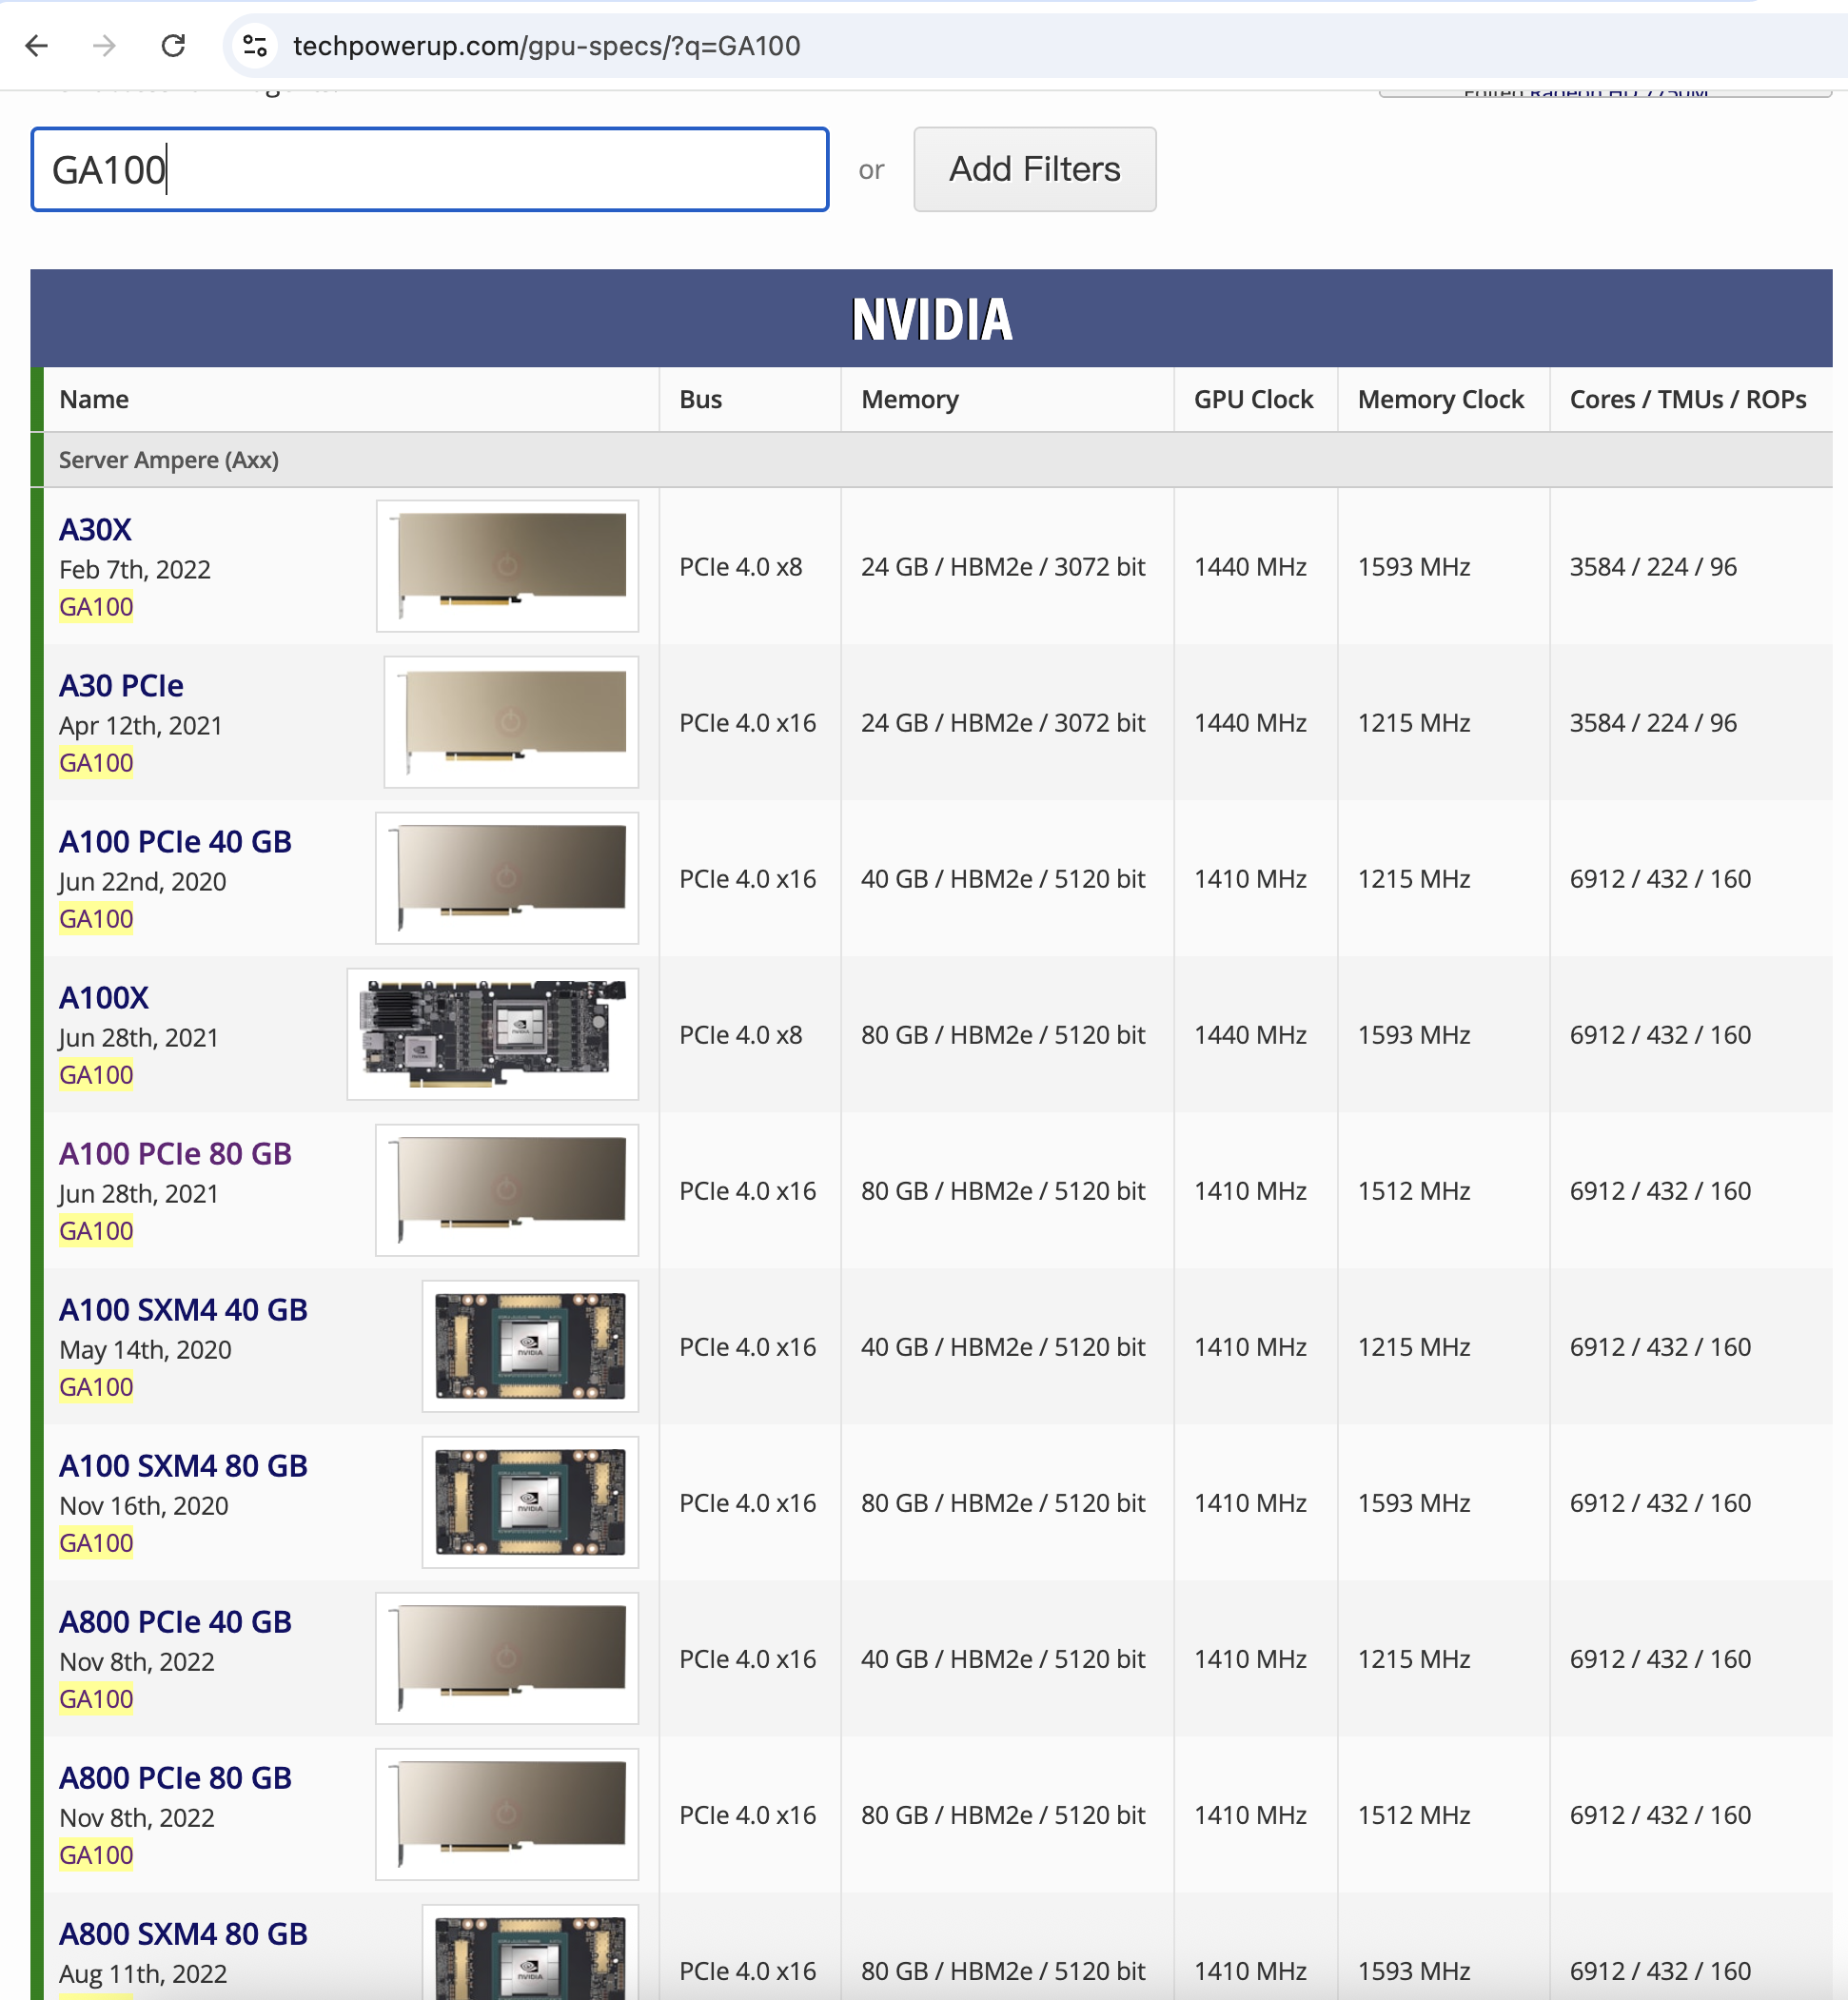
\includegraphics[width=0.75\linewidth]{resources/cuda-020.png}
    \caption{GA100}
    \label{fig:placeholder}
\end{figure}

\subsection{GA102芯片与消费级市场}

另一方面，我们的第二个例子，GA102芯片则更常用于面向普通用户或游戏玩家的GPU。例如该芯片出现在GeForceRTX
系列中专为普通PC或工作站设计。此外，从tech powerup网站这里的这一部分可以看出，这里的大多数GPU都带有散热
风扇。这是一个视觉标志，表明这些GPU是为日常使用设计的，而非用于高性能计算或超级计算机。

\begin{figure}
    \centering
    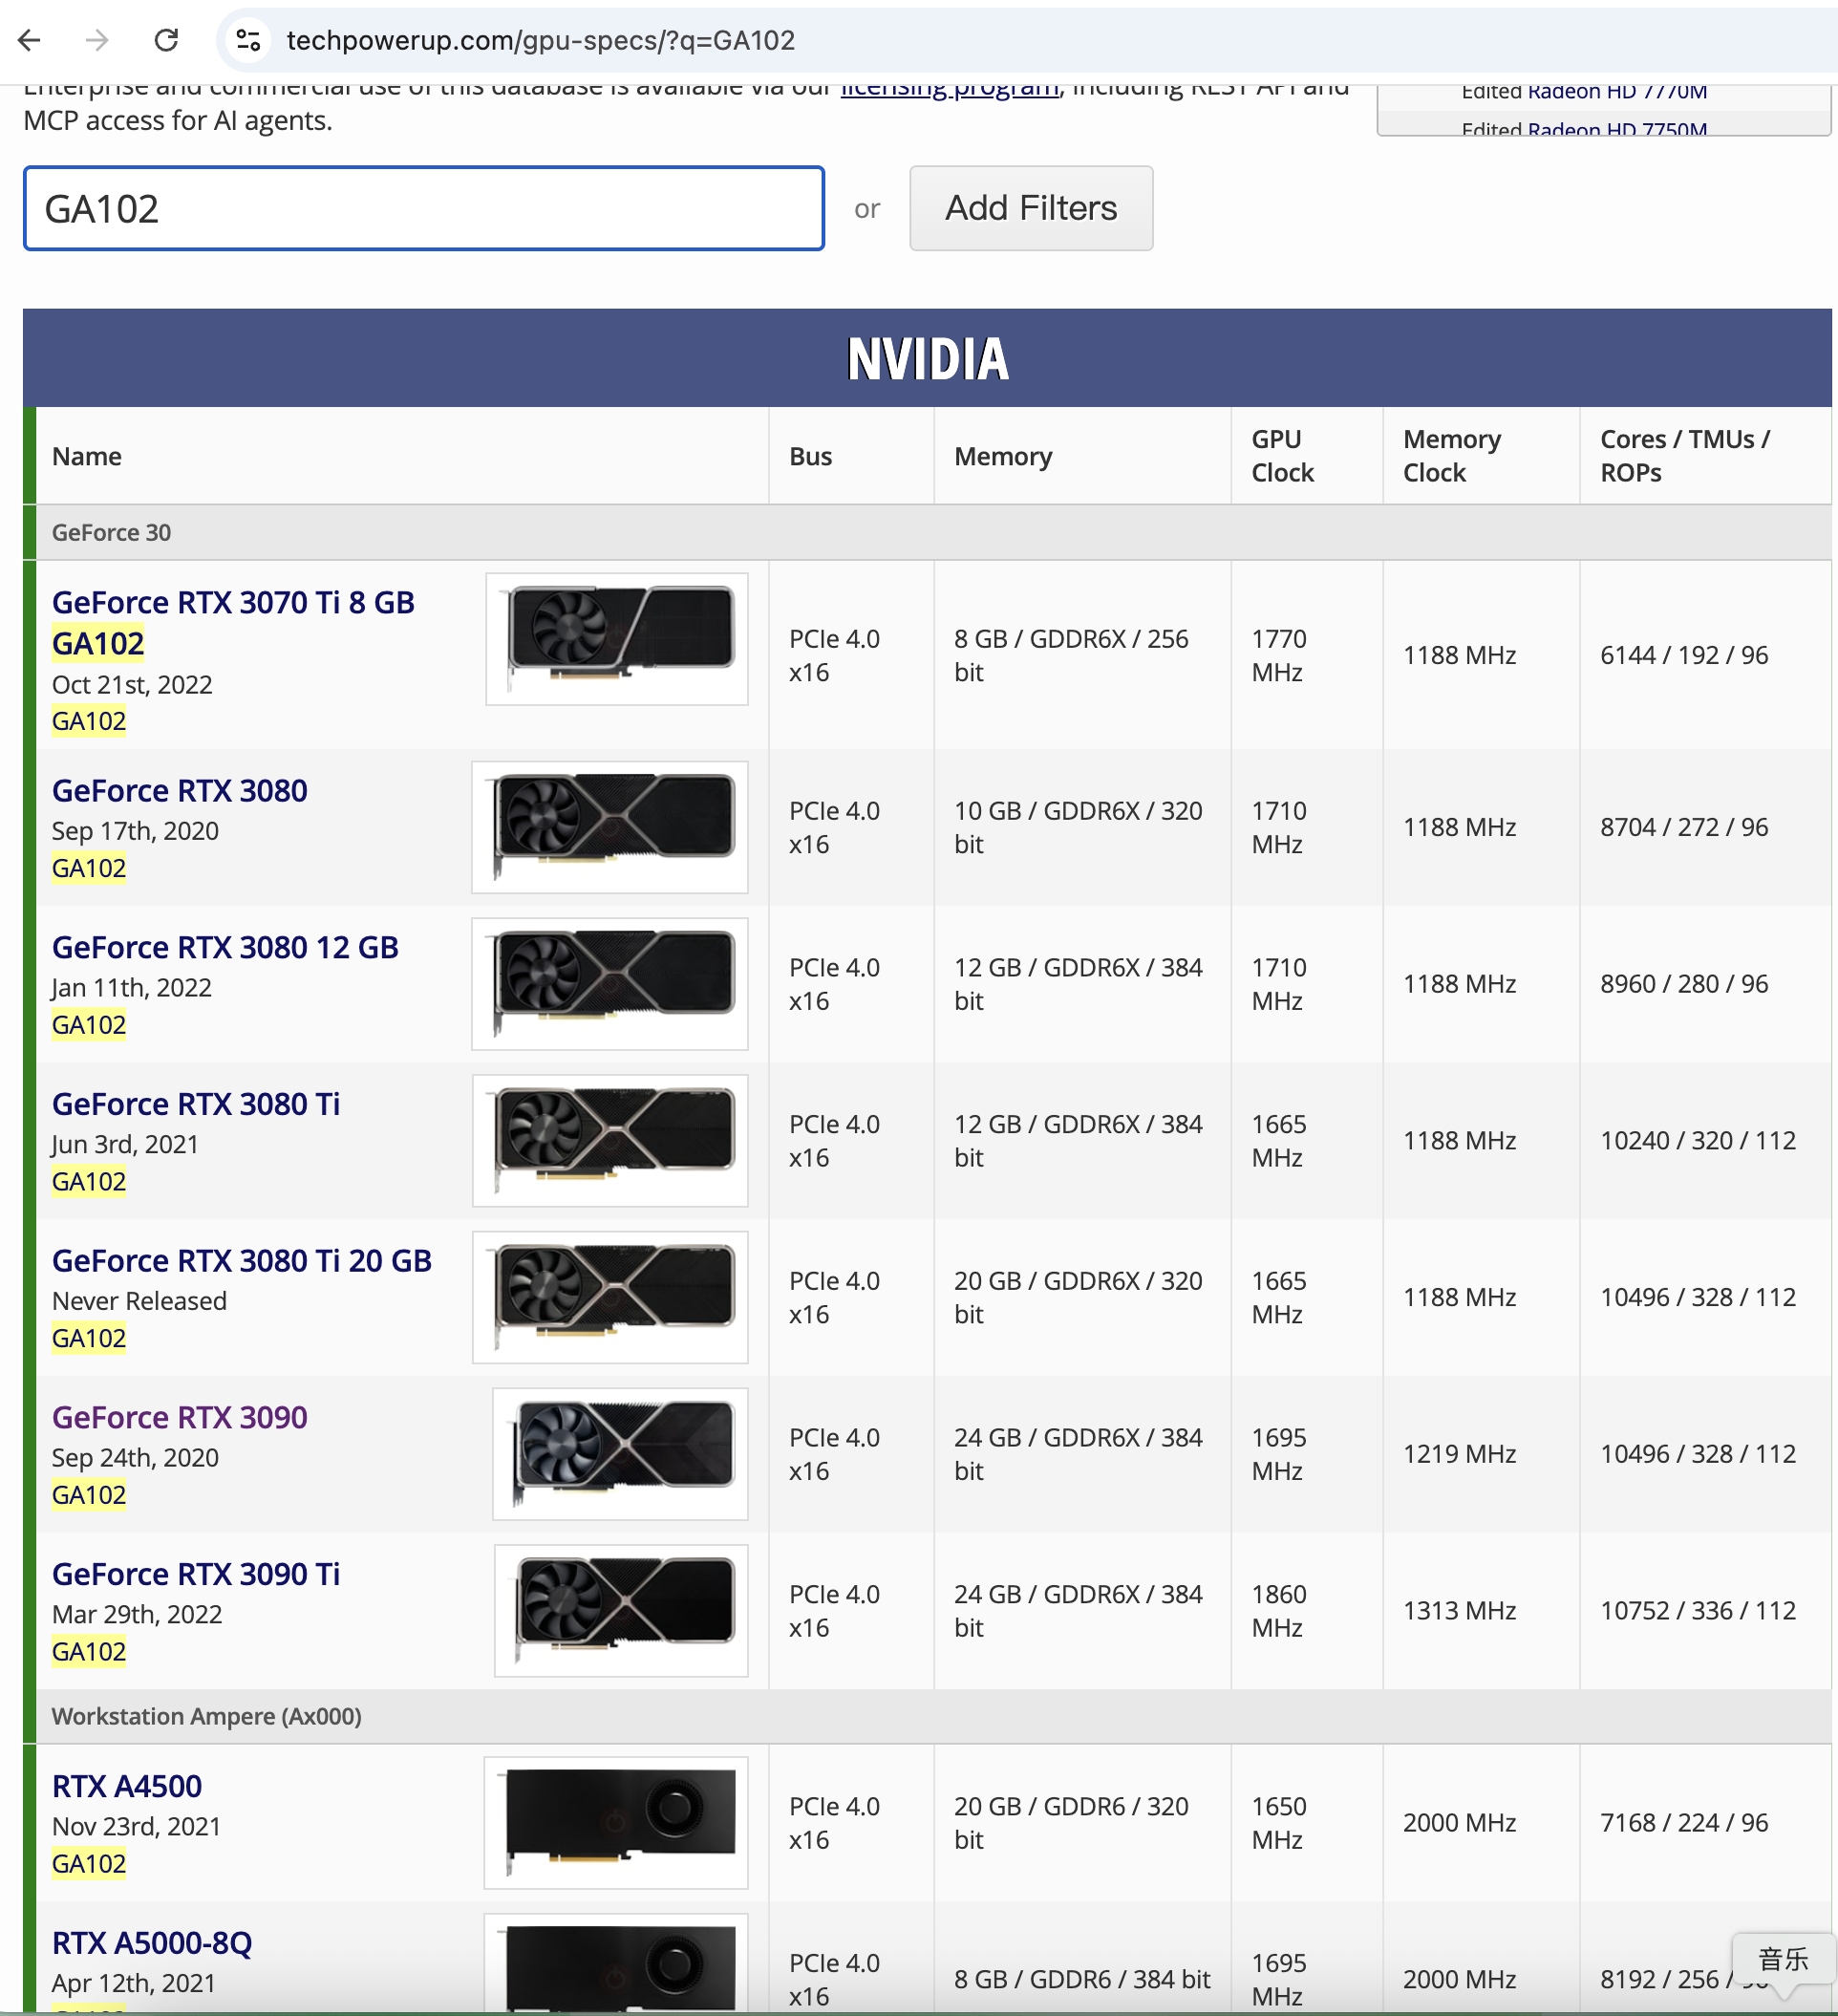
\includegraphics[width=0.75\linewidth]{resources/cuda-021.png}
    \caption{GA102}
    \label{fig:placeholder}
\end{figure}


同样的，如果我们再回到GA100芯片的网页，你会发现它通常用于不带散热风扇的GPU。这表明它被应用于超级计算机和高性能计
算服务器。这些场景通常采用其他更坚固的散热方法或系统，不过这并非总是如此。总结来说，现在已经很清楚某些芯片是专门为高性能
计算应用设计的，而另一些则是为日常消费级用途设计的。

\subsection{芯片的多用途适配}

NVIDIA有时会发布同一芯片的不同版本。例如，以Ampere架构中的一款芯片为例，我们以GA102为例，在其网页上我们
注意到它常用于游戏市场，因为大多数GPU都带有散热风扇，或者你可以打开其中一款GPU搜索其产品系列，结果应该是GeForce。例如，然而，如果我们查看该表格的前几行、前2或3款GPU，会发现这款芯片也被用于设计和制造高性能计算服务器用的GP

U。仔细查看此处这一部分，会发现这是GA102芯片的一个不同版本。它被称为面向高性能计算的版本。这款面向高性能计算的版本
编号为890，而面向游戏市场的版本编号则在100到350之间。

这展示了NVIDIA在将芯片适配多种用途方面的灵活性。我还想强调一点，值得注意的是，每颗芯片以及特定架构内的每个芯片版本
，都可能根据GPU型号甚至制造商的不同，以不同的速度或频率运行。这是因为NVIDIA会向市场上的多家公司提供GPU芯片和
授权，由他们生产GPU，这些公司生产的GPU可能在频率等细节上略有差异。

在本文章的最后，我想再次澄清，我在本课程中的目标是赋予你们独立处理这些主题的知识与技能。请记住，牢固的基础是掌握任何学科
的关键，这可以通过扎实掌握基础知识来实现。正如我们在本期文章以及之前文章中所探讨的内容。


\section{NVIDIA GPU 架构历史}

大家好，在本文章中我将带大家了解NVIDIA推出的各种GPU架构。我们先从这张展示的图像开始，该图像表明自1998年以来
，NVIDIA已推出了众多架构。我们将从NVIDIA于2010年推向市场的Fermi架构开始探索。不过，我们将跳过一些早
期架构，因为它们已不再使用。

\begin{figure}
    \centering
    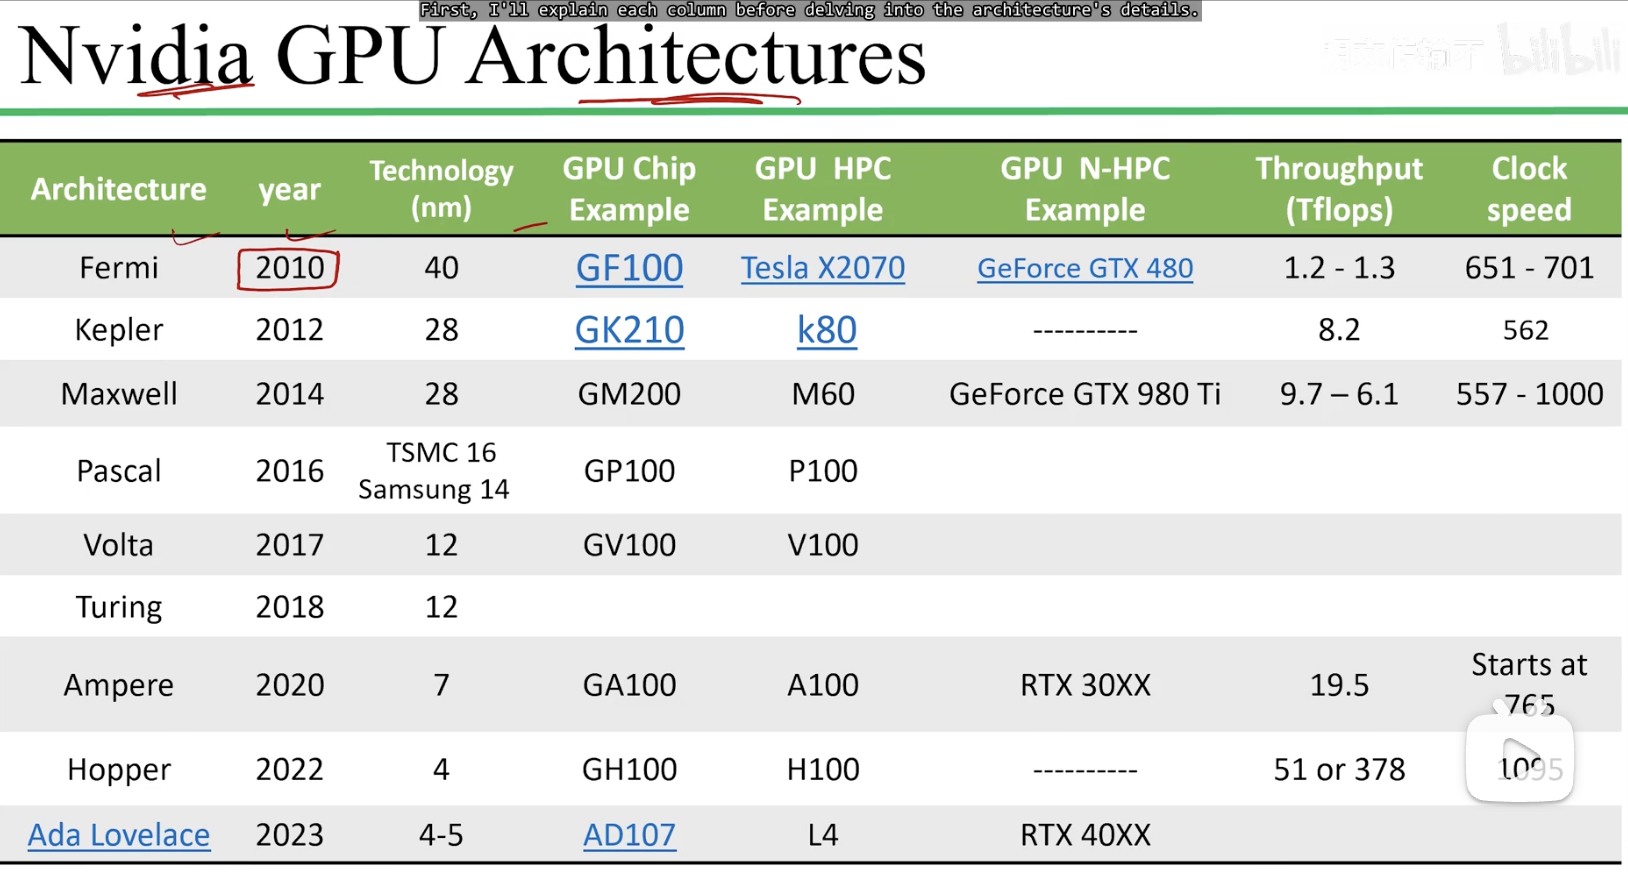
\includegraphics[width=0.75\linewidth]{resources/cuda-022.png}
    \caption{GPU 架构历史}
    \label{fig:placeholder}
\end{figure}


这张展示的表格列出了NVIDIA自2010年以来推出的所有架构。首先，在深入讲解各架构细节之前，我会先解释每一列的含义。
第一列显示了NVIDIA引入的架构名称，第二列显示了他们各自的发布时间。接下来是GPU芯片示例列，该列提供了每个架构的代
表性电子芯片。在后续讲解中，我会为每个架构突出展示两款不同的GPU型号，它们被分为两列，第一列是HPC GPU，即高性能计
算GPU。第二列是非高性能计算GPU，即面向普通用户或普通消费者的GPU。最后，我们还有两列专门用于评估各架构的计算能力
或性能指标。

在本表中，我仅选取了两个关键参数进行比较。第一个是吞吐量，用于计算每秒浮点运算次数。第二个是时钟频率。对于这些参数，在大
多数情况下，我会为高性能计算GPU显示一个数值，为面向普通消费者的GPU显示另一个数值。

\subsection{Fermi架构}

我将深入讲解NVIDIA GPU的各种架构。我们从 Fermi架构开始。Fermi架构由NVIDIA于2010年推出，是
GPU设计与技术的一次重大飞跃。

基于Fermi的GPU采用40纳米工艺制造。一个基于Fermi架构的GPU芯片示例是GF100芯片，该芯片被用于生产多种
GPU，既用于高性能计算，也用于普通用户或普通消费者。另一方面，GeForce GTX 480则专为普通消费者和游戏玩家设计
。例如其中一款高性能计算GPU是基于该芯片或该架构的Tesla X2070。如果你关注这些数字，这些性能指标数字，你可能会
疑惑，为什么专为普通用户设计的GTX480在性能上似乎优于Tesla X2070？在性能指标方面，这两款GPU的吞吐量分别
可达1.2和1.3万亿次浮点运算，每秒TFlops时钟频率分别为655和701 Mhz。例如，GTX 480的时钟频率为
700，而 X2070 GPU仅为651。

\begin{figure}
    \centering
    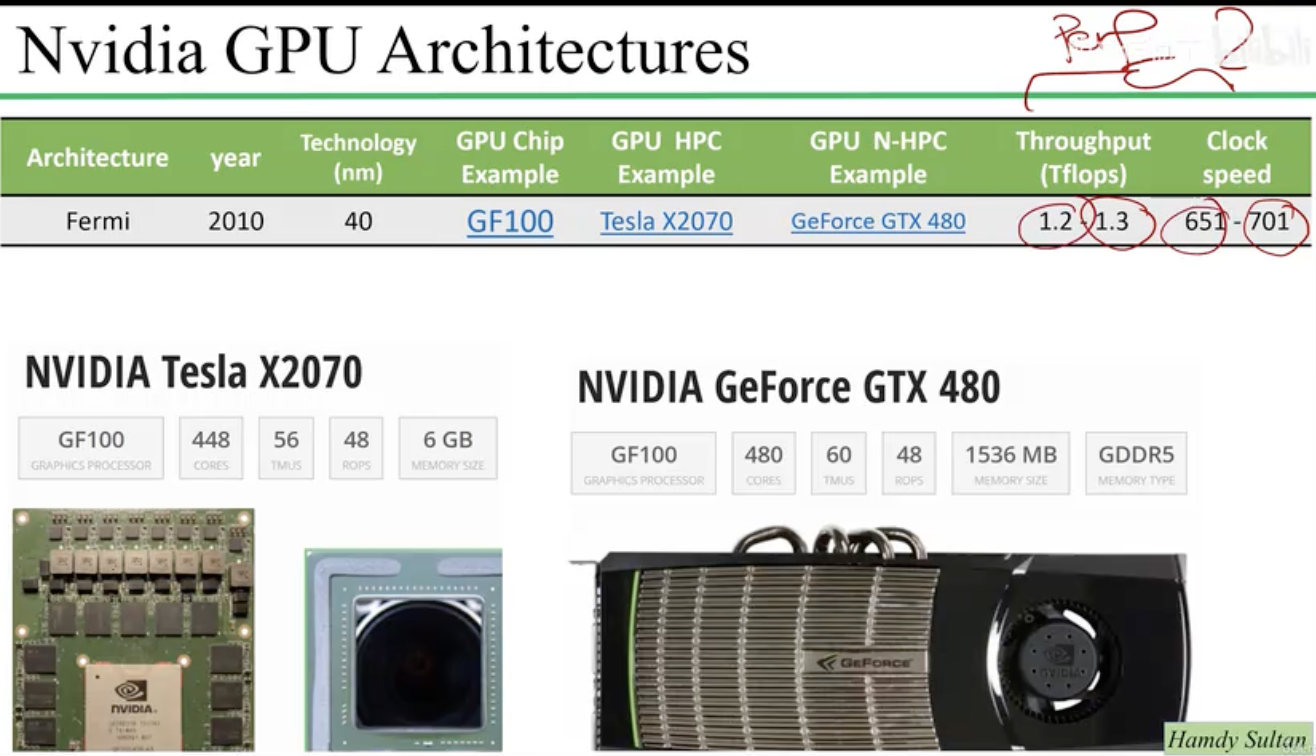
\includegraphics[width=0.75\linewidth]{resources/cuda-023.png}
    \caption{Fermi 架构示例}
    \label{fig:placeholder}
\end{figure}


要解答这一点，必须理解，评估GPU性能并非一目了然。GPU的整体性能受多种因素和指标影响，而不仅仅是这两个指标。仅凭TFlops或时钟频率这样的单一指标不足以全面衡量GPU的整体能力。此外，某一指标看似有意，在另一背景下可能并非如此。例如，

更高的时钟频率虽然能加速任务，但也可能导致功耗和能耗增加，这对某些系统来说可能并不理想。

另外需要澄清的是，GTX GPU看似优于X2070 GPU的TFlops值或吞吐量值，仅针对单精度运算。这并非针对GPU
中所有核心的整体性能。我们通过一个例子深入说明这一点。当我们打开Tech Power UP网站查看这两款GPU时，你会注意
到X2070 GPU的双精度性能，如此处所示约为 582.8 GFLOPS，该数值高于GTX GPU的数值。这表明在双精度
任务方面，X2070 GPU的性能几乎是GTX GPU的四倍。GTX 480 GPU仅有168.1 GFLOPS，这类任务之一
就是科学仿真。然而在纹理和像素填充率等指标上，这些指标需要单精度运算。GTX480 GPU则优于 X2070 GPU，这也
符合其面向图形游戏和日常应用的定位。

\subsection{Kepler架构}

让我们回到幻灯片讲解下一个架构Kepler。在Fermi发布两年后，NVIDIA推出了Kepler架构。观察这一列可以明
显看出NVIDIA大致每一年或两年就会发布一款新架构。Kepler架构采用28纳米工艺制造，而Fermi架构使用的是40
纳米工艺。

NVIDIA的 GK210芯片主要应用于Tesla K80 GPU而闻名，该GPU是一款高性能计算GPU卡。令人意外的是，
Tesla K80 GPU包含两颗芯片，而非一颗在一块板卡上使用了两颗GK210芯片。凭借单板上集成的两颗芯片，K80GPU实现了约8.2万亿次浮点运算每秒的吞吐量。
这相比Fermi架构提升了六倍。但需要注意的是，该吞吐量值包含了两颗芯片的
总和，这意味着每颗芯片及每颗GK210芯片大约提供4.1万亿次浮点运算每秒。除了K80GPU，基于该芯片的其他广为人知的
GPU并不多，大多数面向消费市场的其他Kepler GPU均基于不同的芯片。

\begin{figure}
    \centering
    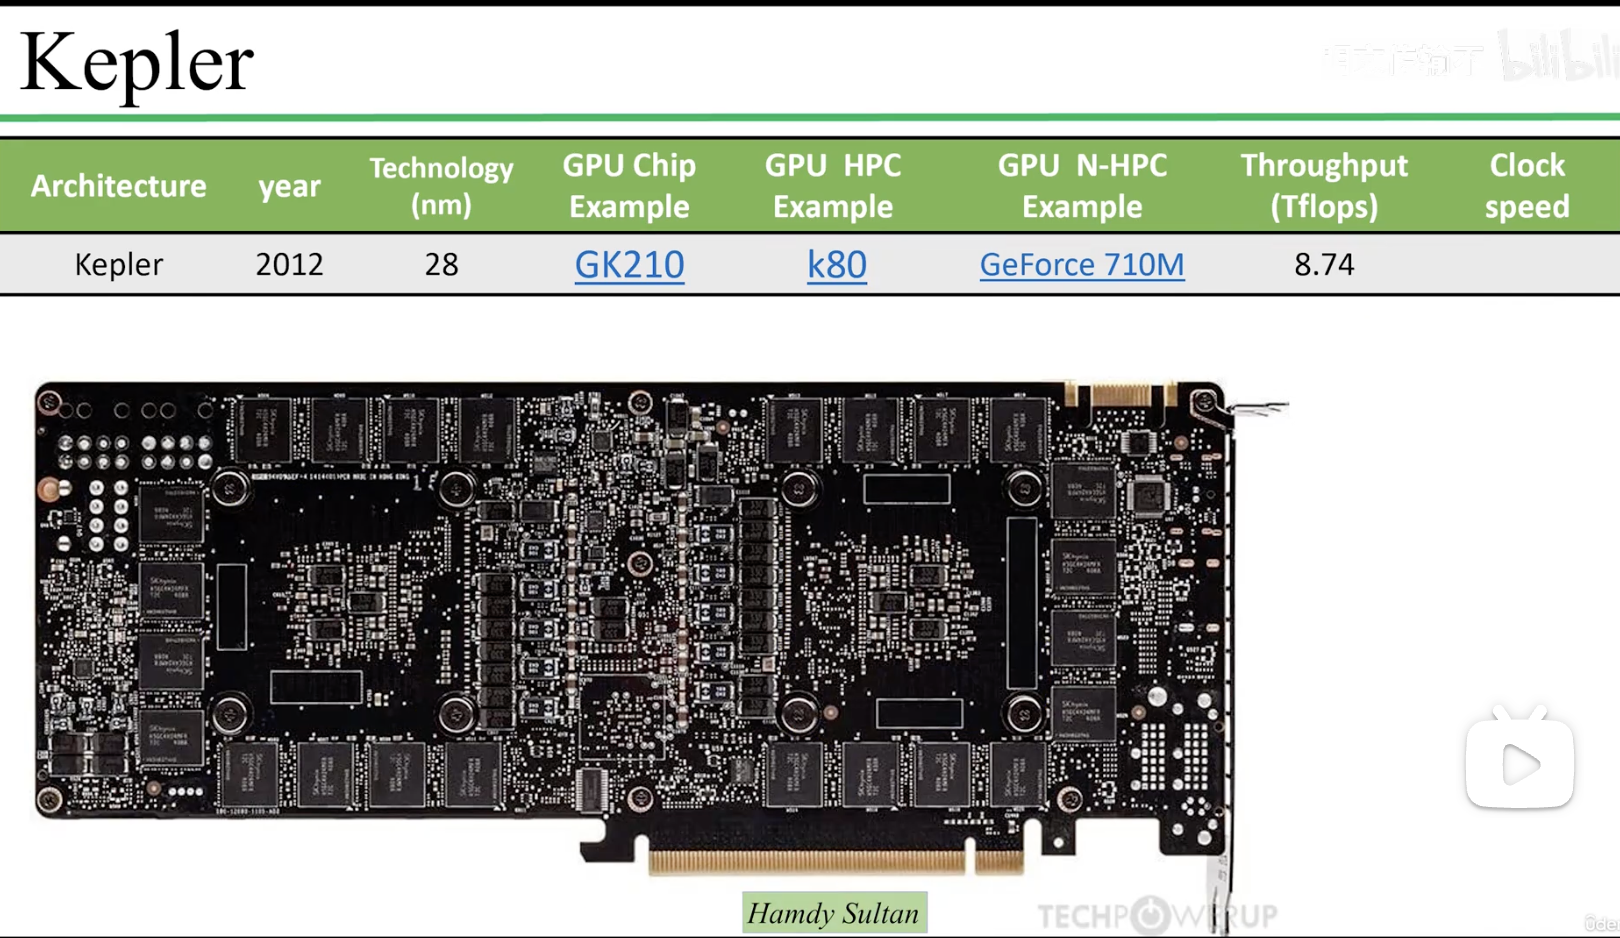
\includegraphics[width=0.75\linewidth]{resources/cuda-024.png}
    \caption{Kepler 架构}
    \label{fig:placeholder}
\end{figure}


关于Kepler，我还想提一下它的升级版本。如需查看基于各类Fermi芯片的更完整GPU列表，
可参考Tech Power UP网站的Fermi专区，有时NVIDIA会发布同一架构的升级版或增强版。例如，Kepler最初由NVIDIA于2012
年推出，但在2013年至2015年间出现了更更新的Kepler版本。如此图所示，你可以看到Maxwell架构也发生了类似
情况，当你在Tech Power APP网站上查看GK210芯片时会发现其发布时间为2014年，与表格中提供的2012年不
同，表格中的发布日期指的是该架构的最初版本。

\subsection{Maxwell架构}

Maxwell架构由NVIDIA于2014年推出，是GPU领域的一项重大进步，它同样采用28纳米工艺制造，该架构的旗舰芯
片之一是GM200，该芯片被用于Tesla M60 GPU，专为高性能计算设计。此外，对于游戏玩家而言，GeForce GTX980 Ti
是另一款基于Maxwell架构的GPU。在吞吐量方面，M60 达到9.7万亿次浮点运算每秒，而GTX GPU
为6.1万亿次浮点运算每秒。在时钟频率方面，M60运行于557兆赫，而GTX则达到1000兆赫。再说一遍，这款专用于高性
能计算的M60时钟频率较低，这直接关联到能耗问题。

\subsection{Pascal架构}

从Pascal架构开始，高性能计算GPU卡采用了字母加100的命名模式。在Pascal架构中，GPU名称为P100，其中
P代表Pascal，这一趋势延续到Volta、Ampere和Hopper架构，它们分别被命名为V100、A100和H100。这种命
名方式也体现在GPU芯片上，如我们所见，Pascal架构中有GP100，随后在Volta、Ampere和Hopper中分别有GV100、GA100和GH100。Pascal架构于2016年推出，采用16纳米和14纳米工艺制造。你可
能会疑惑，为何同一架构会采用两种不同的工艺？主要原因在于当时市场上不同制造商可获得的技术水平不同。有些厂商能使用更先进的
14纳米工艺生产GPU，而其他公司仍在使用16纳米工艺。尽管存在这些差异，各公司仍能基于相同的Pascal架构生产GPU
，只是纳米尺寸不同。

关于Pascal架构，我不会在此过多展开，因为我会在后续文章中结合白皮书或数据手册详细讲解剩余架构。这里只提一点，如我们
所见，性能提升极为显著。只需看看Hopper架构的吞吐量，并将其与Fermi的数值进行比较，一切便一目了然。从Fermi
架构的1.2万亿次浮点运算每秒，到如今Hopper架构的378万亿次浮点运算每秒，我此处略过所写的51万亿次浮点运算每秒
，因为它将在Hopper架构文章中深入解释。


\section{不同架构间的核心对比参数}

本章将深入探讨影响GPU性能的关键参数。理解这些内容将有助于我们后续阅读GPU白皮书和数据手册。

从前几章中，我们已知每一代新架构都在软件和硬件能力上带来了显著进步，在各类领域和应用中提供了更高的性能。一个清晰的例子就是
从 Fermi 架构到 Hopper 架构的吞吐量增长，如下表所示，吞吐量增长超过了300倍。

如果你还记得前文关于 GPU 性能的重要提示，评估性能并非一目了然，它需要理解数十种指标和单位，而不仅仅是吞吐量或速度。
那么，有哪些参数、单位和指标可用于衡量每一代新架构相较于前代的性能？例如，当 NVIDIA 在新架构中增加核心数量时，这是否
足以提升架构性能，还是存在其他因素？为回答这个问题，让我们来看这些关键参数和指标——它们是理解 GPU 性能最关键的要素，
但需注意，它们并非评估 GPU 性能的全部指标，只是最主要的几个。

\subsection{内存带宽}

本章的第一个参数是内存带宽。内存带宽指的是内存每秒能处理多少数据，以 GB/s（每秒千兆字节）来衡量。为了说明内存带宽对应用
性能的影响，我们来讨论以下场景。假设我们有一块 GPU，其全局内存提供的带宽有限。再假设该 GPU 包含四个核心，而这块内存每
秒只能提供 32 位数据。每个核心都需要从该内存读取 32 位数据，所需数据总量为 128 位。那么问题是：这块内存能否在一秒内处理
全部四个请求？

\begin{figure}
    \centering
    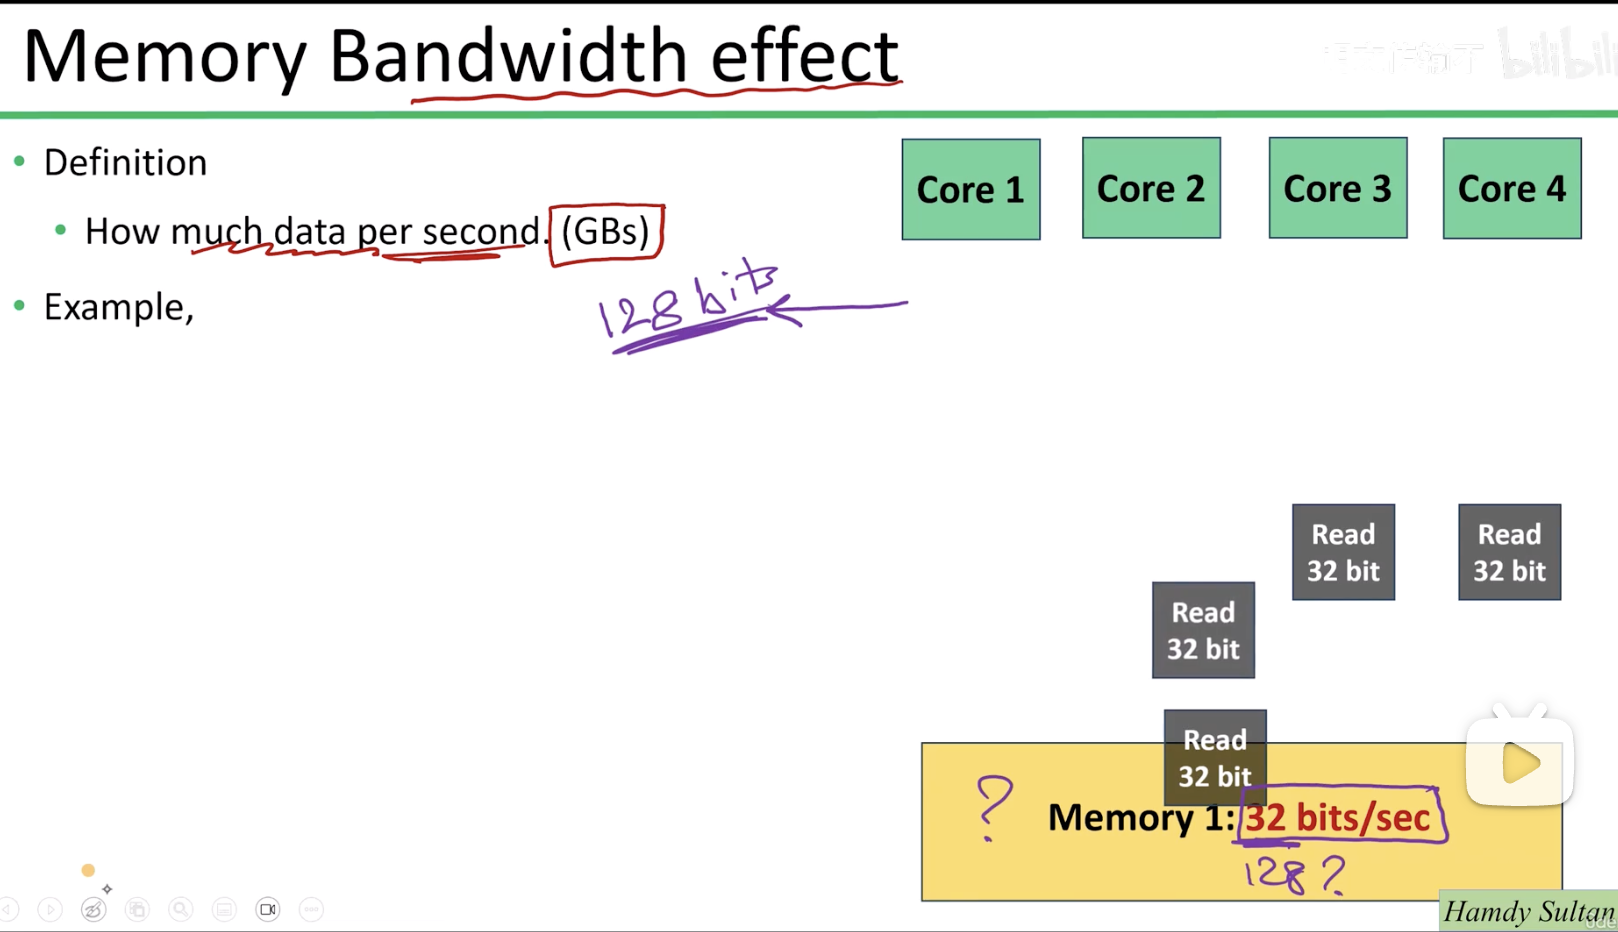
\includegraphics[width=0.75\linewidth]{resources/cuda-025.png}
    \caption{带宽}
    \label{fig:placeholder}
\end{figure}


不幸的是，答案是否定的。由于最大带宽为每秒32位，该内存一次只能处理一个请求。它在第一秒处理第一个请求（前32位），完成后
再继续下一个请求，依此类推。这种串行处理意味着内存需要总共4秒才能响应所有读取请求。

\begin{figure}
    \centering
    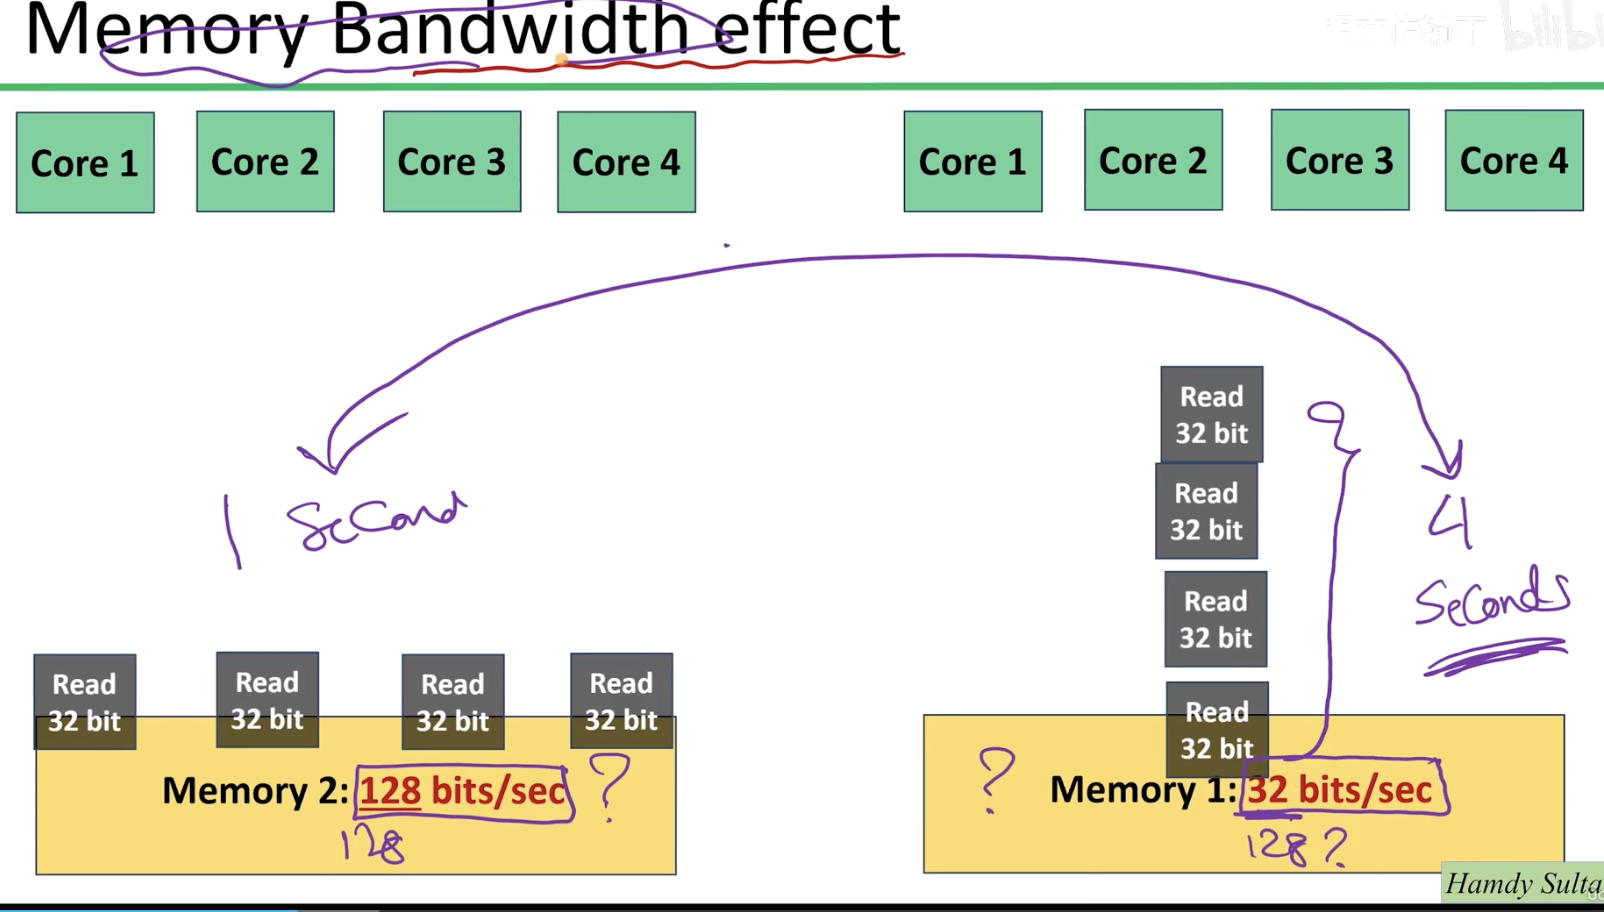
\includegraphics[width=0.75\linewidth]{resources/cuda-026.png}
    \caption{带宽}
    \label{fig:placeholder}
\end{figure}


现在我们将其与另一种带宽更高的内存进行比较。假设我们有一块带宽为每秒128位的内存，同样有来自四个核心的四个读取请求。该
内存的更高带宽可以在一秒内传输128位，这意味着它能在一秒内响应全部四个请求。这充分说明了内存带宽在提升GPU性能中的关键
作用——相比第一块内存，高带宽显著减少了读写操作所需的时间。

从实际角度来看，考虑视频编辑或三维渲染这类带宽密集型应用，更高的内存带宽会使这些应用或任务效率显著提升。在游戏领域，每一
毫秒都至关重要，更高的内存带宽意味着更流畅的帧率和更沉浸的体验，同时也有助于减少延迟。总结一下，更高的带宽使GPU能一次
处理更多数据，从而提升性能。

你可能会疑惑，为什么这里的带宽会与内存速度和总线宽度并列？答案是这两个因素会直接影响内存带宽。为说明这一点，让我们深入看
看总线宽度对内存带宽的影响。


\subsection{总线宽度}

计算机架构中总线宽度的概念可以类比为道路上的车道数量。如果我们把每份数据看作一辆汽车，那么总线宽度就是这些汽车可通行的车
道数量。考虑两种不同场景：第一种场景假设我们有2位总线宽度，相当于一条双车道的道路，因此一次能通过检查点的汽车数量是两辆
。如果每条车道的限速是每秒一辆车，那么在道路尽头的检查点，一秒内总共能通过的汽车数量就是两辆——因为有两条车道，每条车道
每秒一辆车。

\begin{figure}
    \centering
    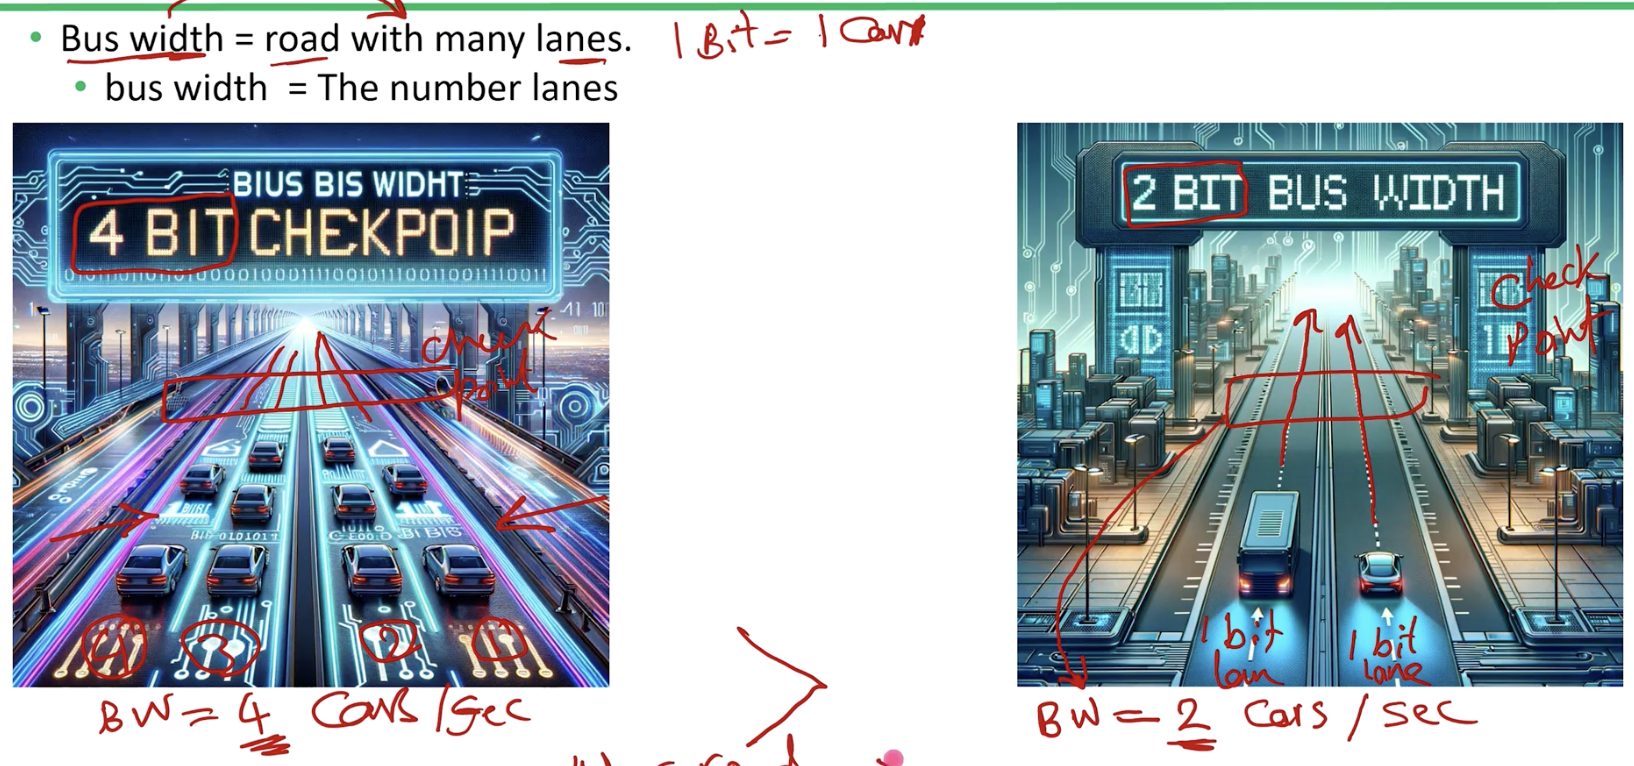
\includegraphics[width=0.75\linewidth]{resources/cuda-027.png}
    \caption{带宽}
    \label{fig:placeholder}
\end{figure}


这条路可让两辆车同时通过检查点，该检查点的带宽是每秒两辆车。第二个例子，假设我们有4位总线宽度，即一条四车道道路。采用相同的限速（每秒一辆车），这条路每秒能处理四辆车。第一条路（2
位总线）的带宽是每秒两辆车，第二条路（4位总线）的带宽是每秒四辆车。总结这两个例子：更宽的总线宽度带来更高的带宽。

现在让我们回到计算机术语，应用同样的类比：将总线宽度翻倍，例如从32位提升到64位，会增加在给定时间内可传输的数据量。但
这仅在内存速度相同的情况下才成立。在同样语境下，内存速度通常称为内存时钟频率，也是GPU性能的关键因素。更高的内存速度使
GPU能更快地访问和处理数据，从而减少瓶颈。关键不仅在于可用内存有多少，更在于内存运行得多快，这对数据密集型任务的整体效
率至关重要。

在之前的类比中，假设每条车道由一名警官管理。检查点的效率不仅取决于道路宽度（车道数量），还关键取决于每名警官检查一辆车的
速度有多快。如果每名警官工作效率更高，能更快地检查每辆车，自然就能在给定时间内让更多车辆通过检查点。

这个类比直接对应GPU中内存的工作方式。如果内存具备更高的速度，就能在特定时间范围内处理更多数据、事务或操作，从而有效提
升内存带宽。正如检查点上效率更高的警官能带来更顺畅、更高效的车流，GPU中更高的内存速度也会带来更大的内存带宽。这种增强
的带宽对GPU整体性能至关重要，因为它决定了数据从内存传输到计算单元（核心）的速度有多快。

\begin{figure}
    \centering
    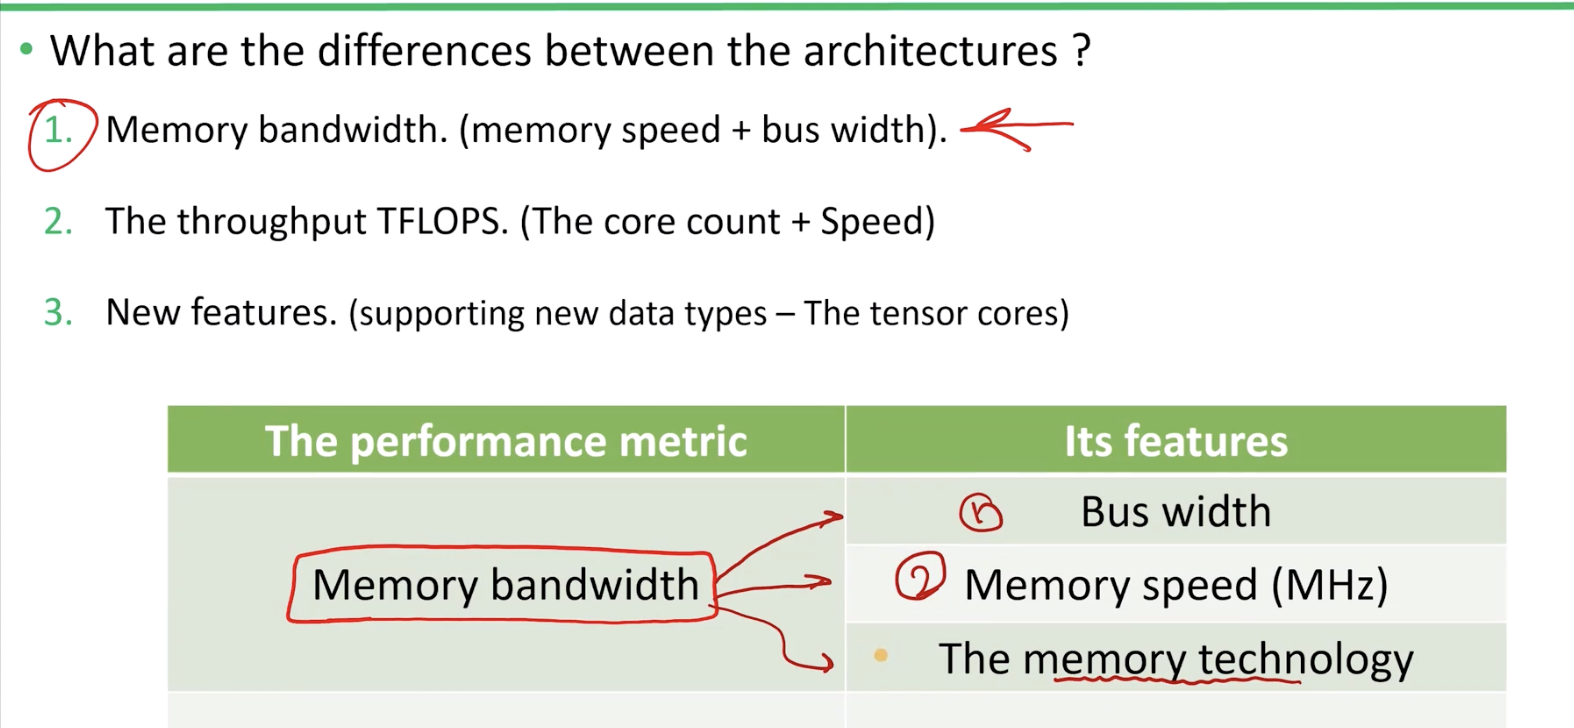
\includegraphics[width=0.75\linewidth]{resources/cuda-028.png}
    \caption{带宽}
    \label{fig:placeholder}
\end{figure}


我们在此考察的指标是内存带宽。现在来总结一下：该指标会受到不同因素的影响，例如内存速度、内存总线宽度以及内存技术（DDR4、
DDR5、DDR6，甚至更新的HBM等）。现在让我们在两款属于不同类别的GPU上检验这一指标及其影响因素。这两款GPU分别是
来自Tesla系列的A100和来自GeForce系列的RTX 3090，如果你还记得我们之前的讨论，Tesla系列专用于高性能计算，而
GeForce则面向游戏和普通用户。需要再次指出的是，这两款GPU都基于Ampere架构，因此它们共享相同的架构，但面向不同的应用场景。

\begin{figure}
    \centering
    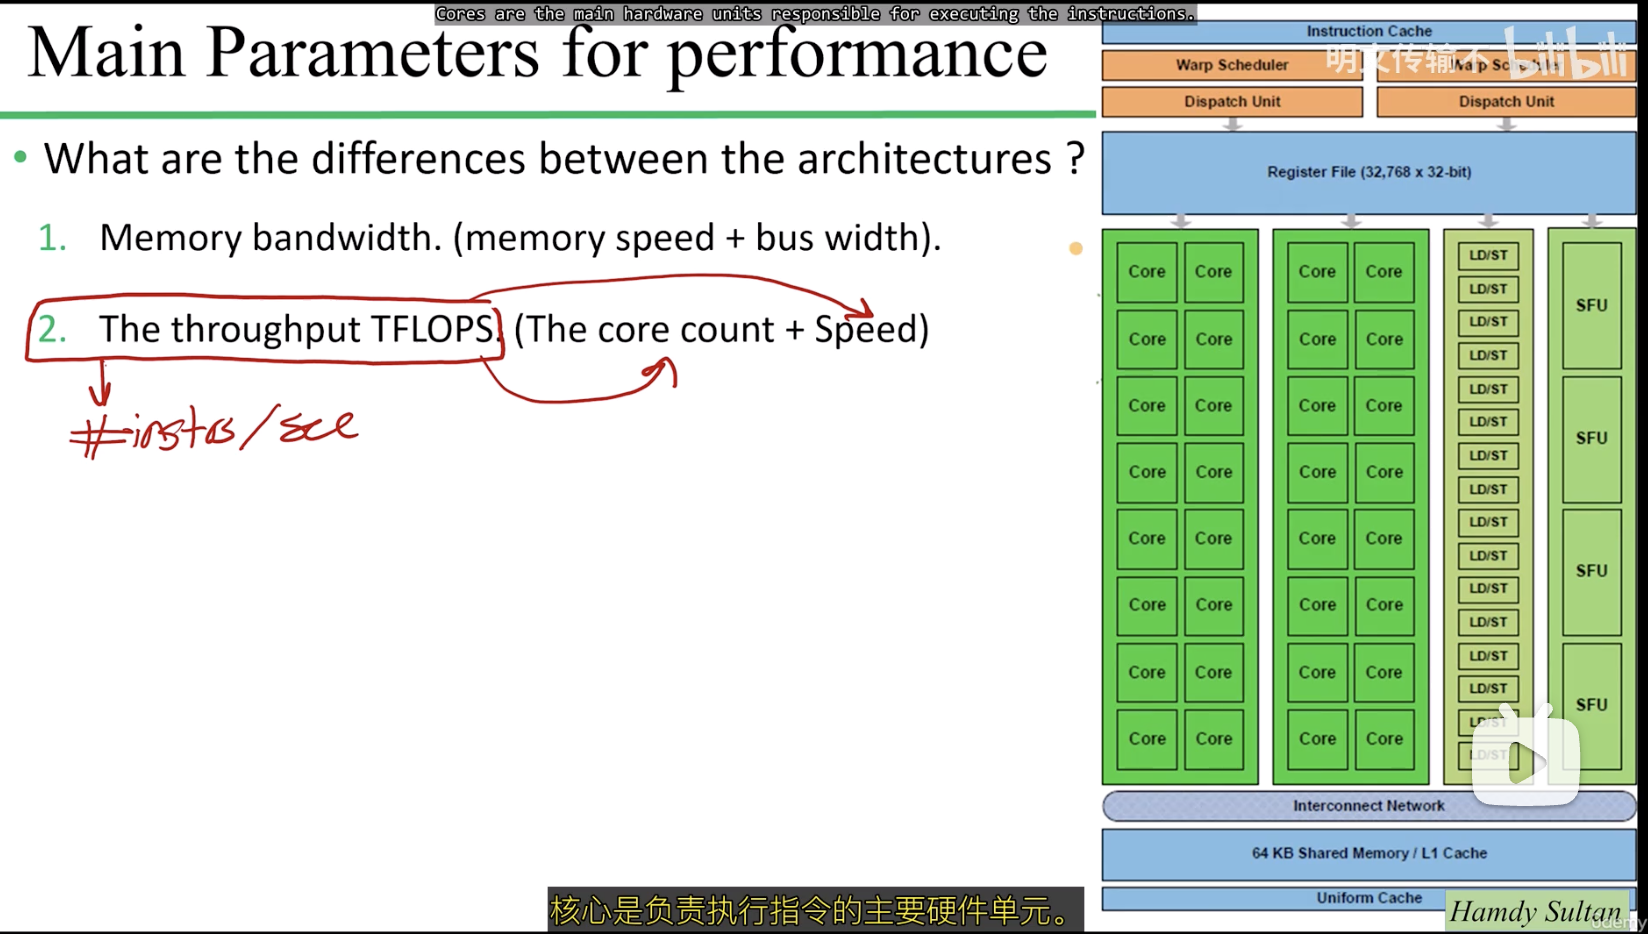
\includegraphics[width=0.75\linewidth]{resources/cuda-029.png}
    \caption{带宽}
    \label{fig:placeholder}
\end{figure}


在高性能计算A100 GPU中，我们观察到其内存总线宽度异常宽——超过5000位，即5000条车道。为便于理解，我们将此数值与
RTX 3090的总线宽度进行比较。尽管共享相同架构，RTX 3090 GPU的总线宽度却只有约400位。你看到差别了吗？A100是5000
位，而RTX 3090只有400位，两者差距超过十倍。此外，当考察内存速度时，它们大致相当。但当我们综合这些因素——内存速度、
总线宽度以及内存技术——就会发现A100 GPU在内存带宽方面显著优于RTX 3090。

在A100中，我们使用了名为HBM2的内存技术，而在RTX 3090中则使用了另一种名为GDDR6的技术。
在介绍下一个参数之前，先思考一个问题：你认为 GPU 中包含的核心数量是否直接影响其性能？来看一个例子，假设需要比较两
款GPU，第一款有100个核心，第二款有200个核心。我们能否说第二款性能更好？

\begin{figure}
    \centering
    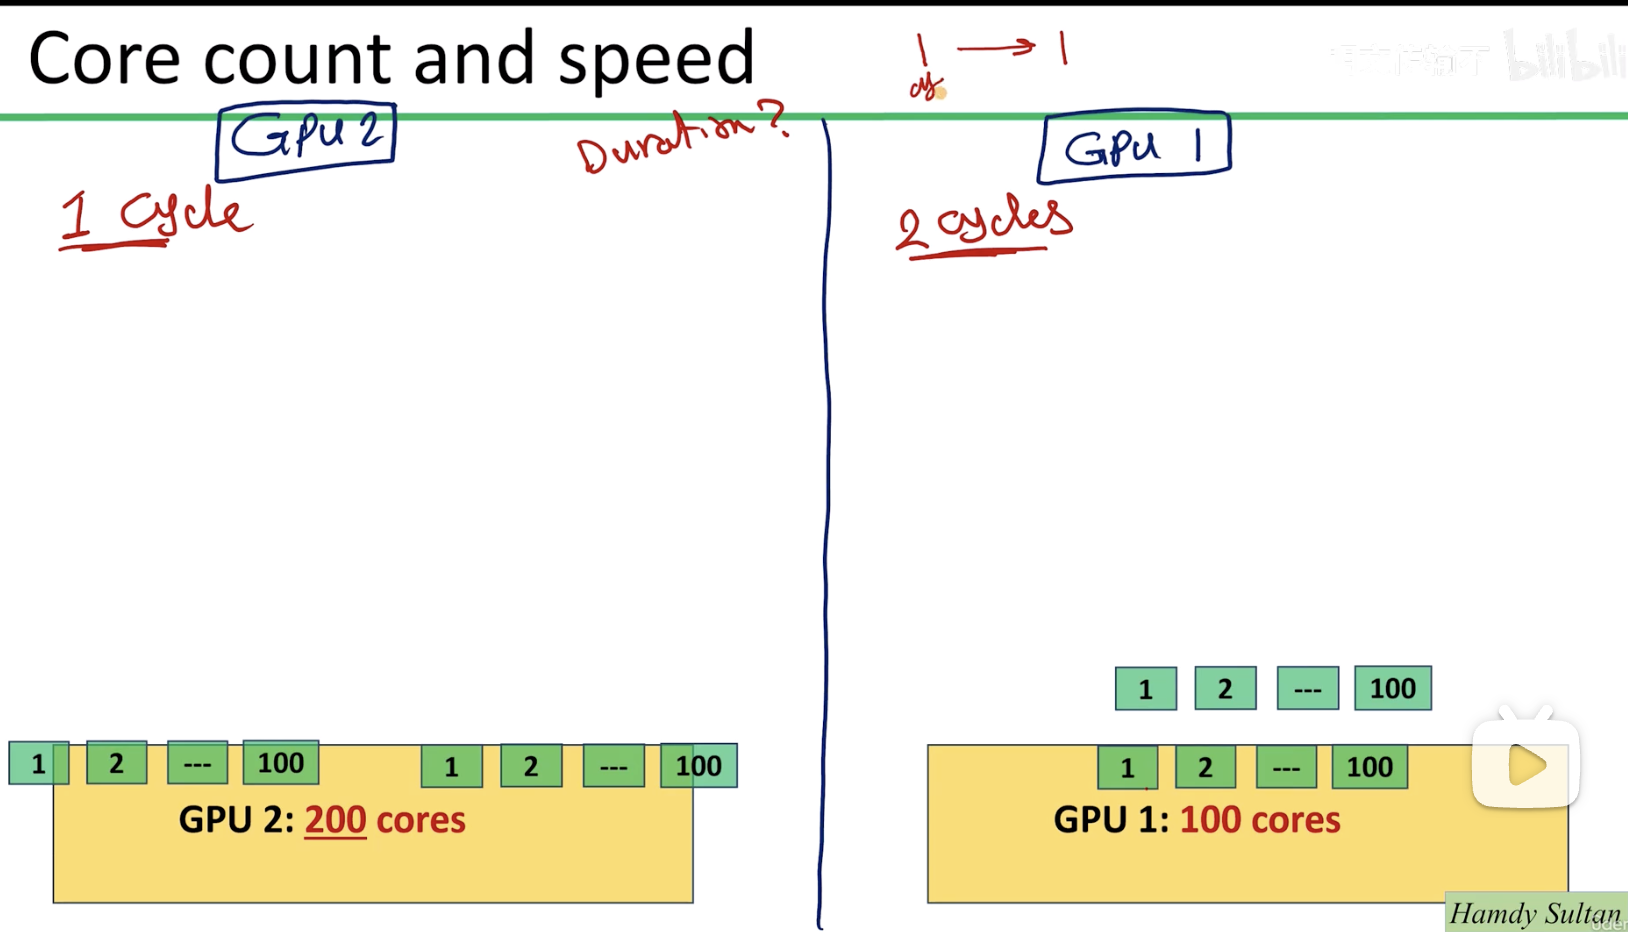
\includegraphics[width=0.75\linewidth]{resources/cuda-030.png}
    \caption{带宽}
    \label{fig:placeholder}
\end{figure}

\subsection{指令吞吐量}

我将通过讲解第二个参数——指令吞吐量——来回答这个问题。在此上下文中，吞吐量指的是整个GPU每秒执行的指令总数。该指
标直接受两个因素影响：核心数量和核心速度，是评估和比较不同GPU型号的关键度量。

为更深入理解这一概念，让我们考虑GPU中核心的作用。核心是负责执行指令的主要硬件单元，更多的核心允许同时执行更多指令，从
而带来更高的吞吐量。为具体说明，假设有两款不同的GPU，一款配备100个核心，另一款配备200个核心。再假设有一个包含200条
指令的应用程序，当该应用程序在两款GPU上运行时，第一款GPU将为每个核心分配一条指令，在第一个周期中处理100条指令，然
后将剩下的100条指令再次分配给各核心。


在第二款GPU的场景中，200条指令将在一个周期内执行完毕，因为我们有200个核心，每个核心接收一条指令。这使得GPU仅用一个
周期而非两个就能完成整个应用程序，性能相较第一款GPU提升了一倍。更高的核心数量意味着更强的并行处理能力，从而实现更快、
更高效的任务执行，尤其适用于可有效并行化的应用程序。这个例子突显了核心数量对GPU吞吐量的重大影响，但这并非绝对真理——在
某些情况下，第一款GPU（核心更少）的性能可能优于第二款GPU。

\begin{figure}
    \centering
    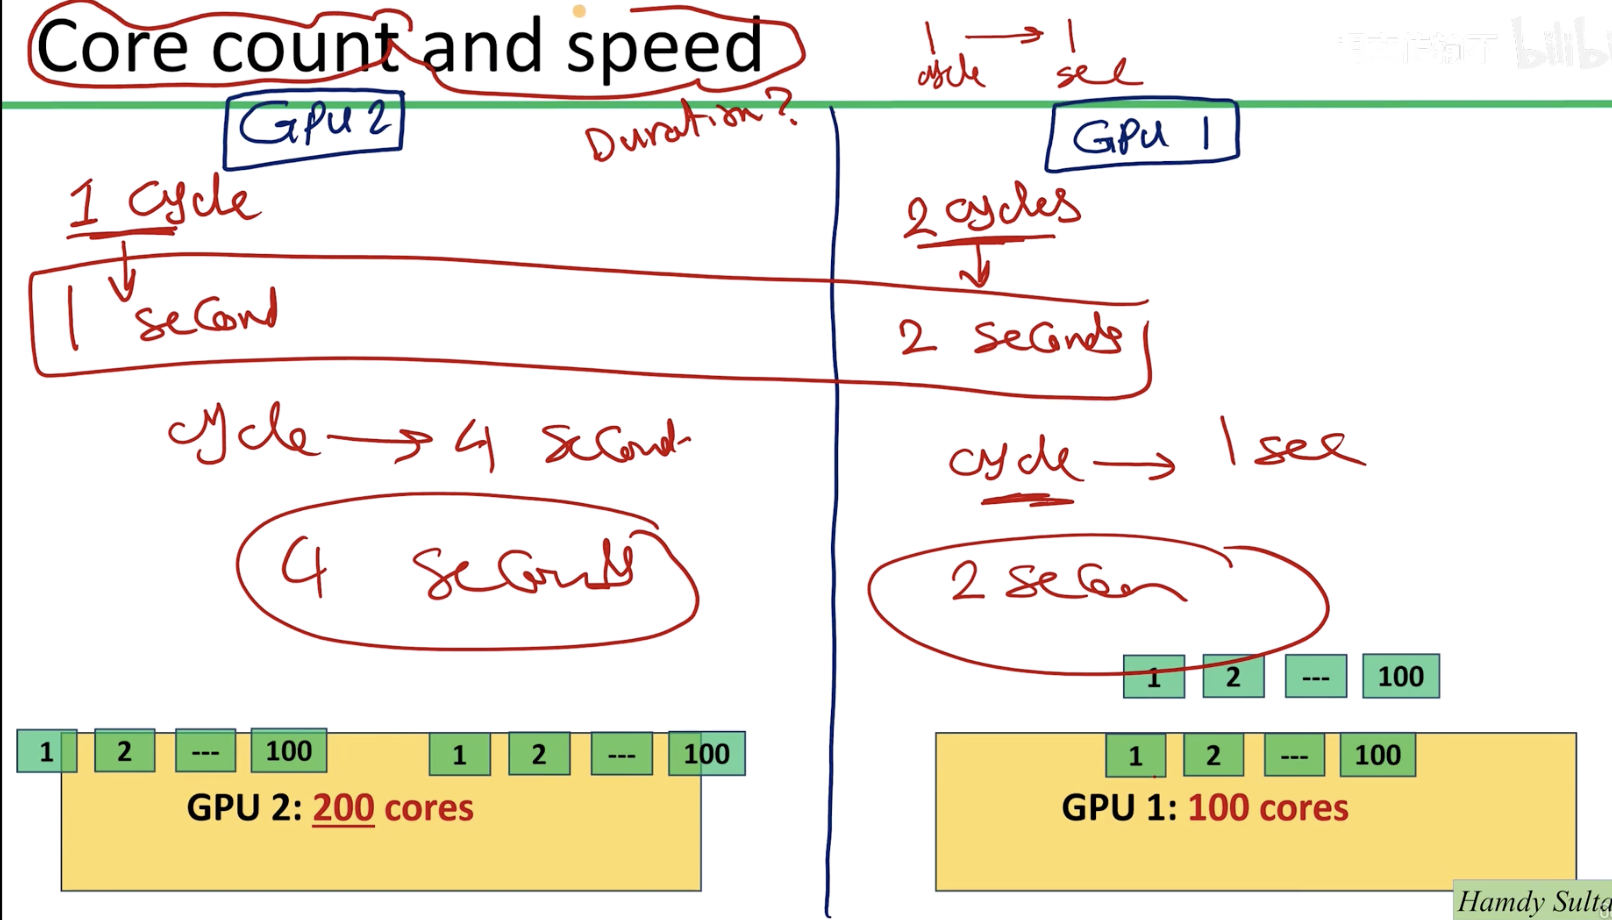
\includegraphics[width=0.75\linewidth]{resources/cuda-031.png}
    \caption{带宽}
    \label{fig:placeholder}
\end{figure}

让我们回顾这个例子：第一款GPU需要两个周期来执行整个应用程序，而第二款GPU只需一个周期。然而，如果我们不知道两款GPU中
每个周期的持续时间，我们的比较就缺乏上下文。为说明这一点，再考虑一个假设：如果第一款GPU每个周期耗时1秒，而第二款GPU
每个周期耗时4秒呢？在这种情况下，第一款GPU将在2秒内完成，而第二款GPU需要4秒。


这一场景凸显了GPU架构中的一个关键方面：核心数量与核心时钟频率之间的平衡。时钟频率——即每个核心执行指令的速率——同样至
关重要。核心数量确实影响同时处理多条指令的能力，这是GPU并行处理的基本原则。但更高的时钟频率意味着每个核心能更快完成分
配的任务，这在需要快速处理复杂小任务的应用中尤为关键。我们可以通过吞吐量这一指标——即单位时间内可执行的指令数量（如每秒
）——来衡量它们对性能的综合影响。

\begin{figure}
    \centering
    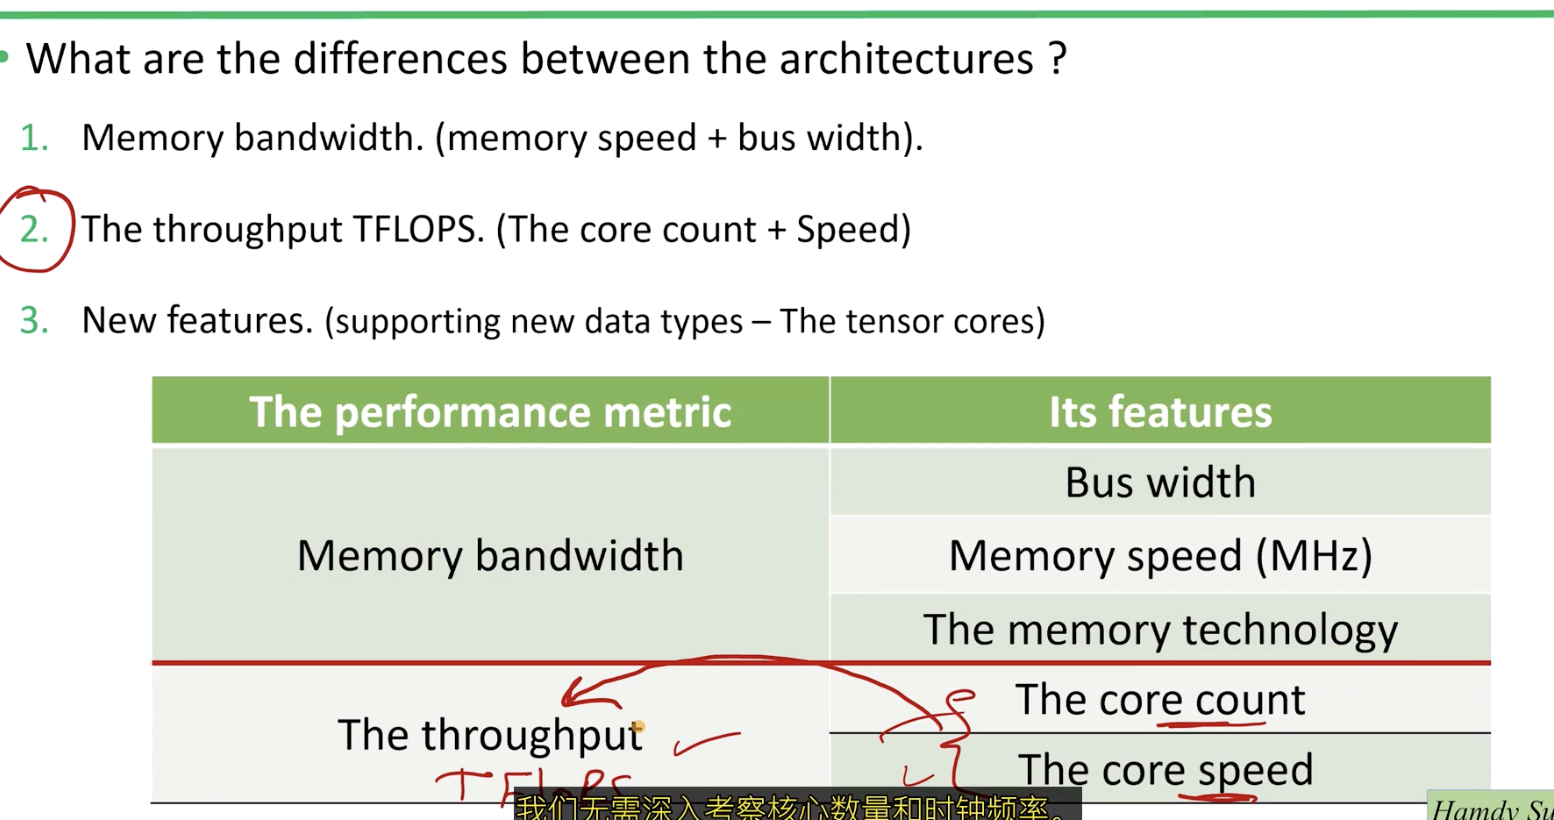
\includegraphics[width=0.75\linewidth]{resources/cuda-032.png}
    \caption{带宽}
    \label{fig:placeholder}
\end{figure}

总结一下，核心数量加上核心速度是重要的硬件特性。在查阅白皮书或数据手册时，我们可以直接关注吞吐量指标，而不必深入考察核心
数量。它们固然重要，但关注吞吐量可以绕过对核心数量和时钟频率的逐一分析。不过时钟频率始终对能耗有重要影响。

\subsection{能耗权衡}

让我们探讨另一个关键问题——这一点非常重要。假设我们有两款 GPU，第一款 GPU 不仅核心数量更多、核心频率更高，其运行速度
也快于第二款。第一款 GPU 在核心数量和速度上都强于第二款，这是否自动使其成为更优选择？根据之前的讨论，你可能会初步认为：
更多的核心、更高的速度，还需要什么呢？

然而，还有另一个关键因素需要考虑——能耗。更高的速度加上更多的核心数量会导致更高的能耗。如果一家公司优先考虑能效（这通常
与节省成本相关），它可能会选择第二款GPU，尽管其规格较低。这一场景体现了一种权衡：如果你想要更高的计算能力和速度，就
必须承担更高的能耗成本，反之亦然。如果我问你哪款GPU更优越，你的回答应该是一个反问——在什么上下文中？你是考虑能效还是
计算能力？

评估GPU性能时，最后一个要考虑的参数是新架构中引入的新特性或硬件单元。


\begin{figure}
    \centering
    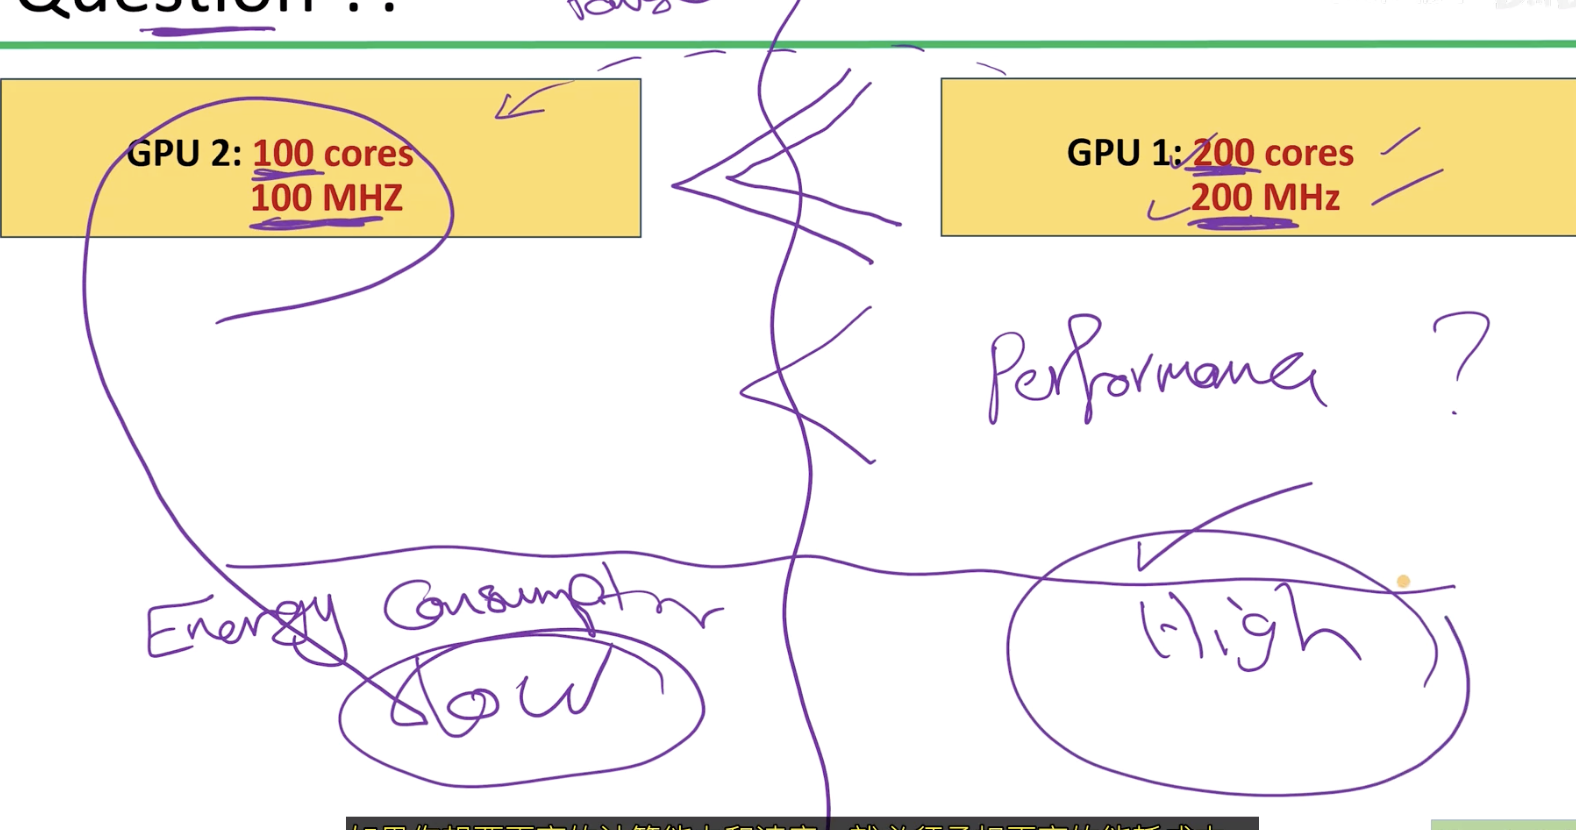
\includegraphics[width=0.75\linewidth]{resources/cuda-033.png}
    \caption{带宽}
    \label{fig:placeholder}
\end{figure}

\subsection{新特性}

有时一个新单元能显著增强GPU的计算能力。例如，NVIDIA在2017年推出的Volta架构中加入了张量核心（Tensor Core）。请看这张
图，它展示了从Pascal到Volta的性能飞跃——同一应用的性能大约提升了八倍。请想象一个复杂的人工智能应用，通常需要消耗八天的
计算资源；而在Volta架构中，借助张量核心，同样的任务可能只需一天即可完成。这个例子突显了张量核心作为硬件单元在GPU计算领
域中的革命性影响。顺便一提，本课程中有专门章节讲解张量核心及其使用方法。

\begin{figure}
    \centering
    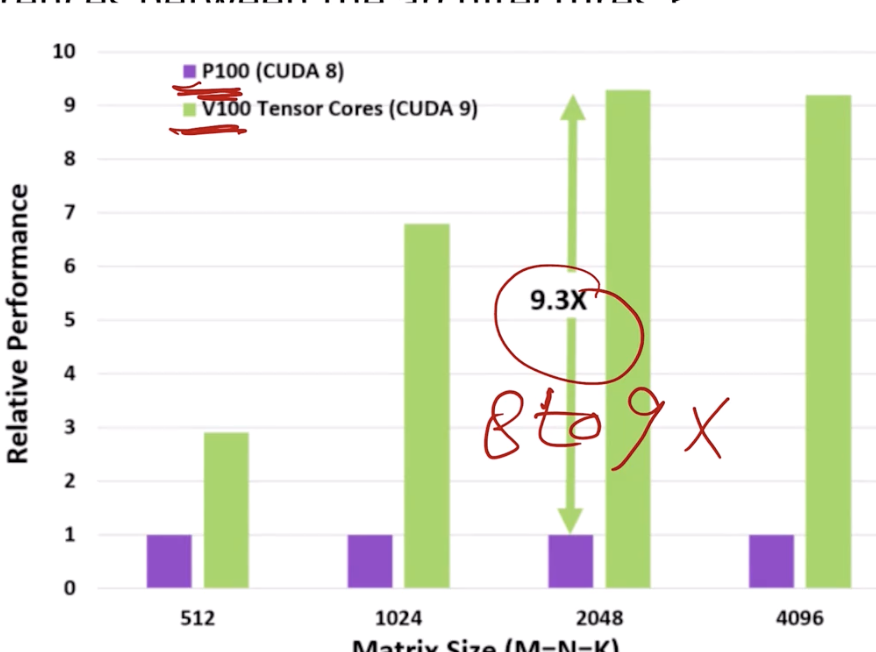
\includegraphics[width=0.75\linewidth]{resources/cuda-034.png}
    \caption{带宽}
    \label{fig:placeholder}
\end{figure}

本章最后，让我们来看一下 NVIDIA 所有白皮书和数据手册中都存在的一张表格。在这张表格中你会注意到列出了大量特性和指标——这
些行提供了关于各种数据类型（从浮点到整数运算）的核心数量信息。然而，正如我们讨论过的，仅看核心数量可能无法全面反映情况
：理解核心速度与核心数量同样重要。或者我们可以直接关注指令吞吐量来简化分析，该指标以 TFLOPS（每秒万亿次浮点运算，即 
\(10^{12}\) 次浮点运算/秒）来衡量。在接下来的章节中，我们将基于本章的讨论，深入探讨最新 GPU 的规格，这些规格来自白皮书和
数据手册中的架构信息。

\begin{figure}
    \centering
    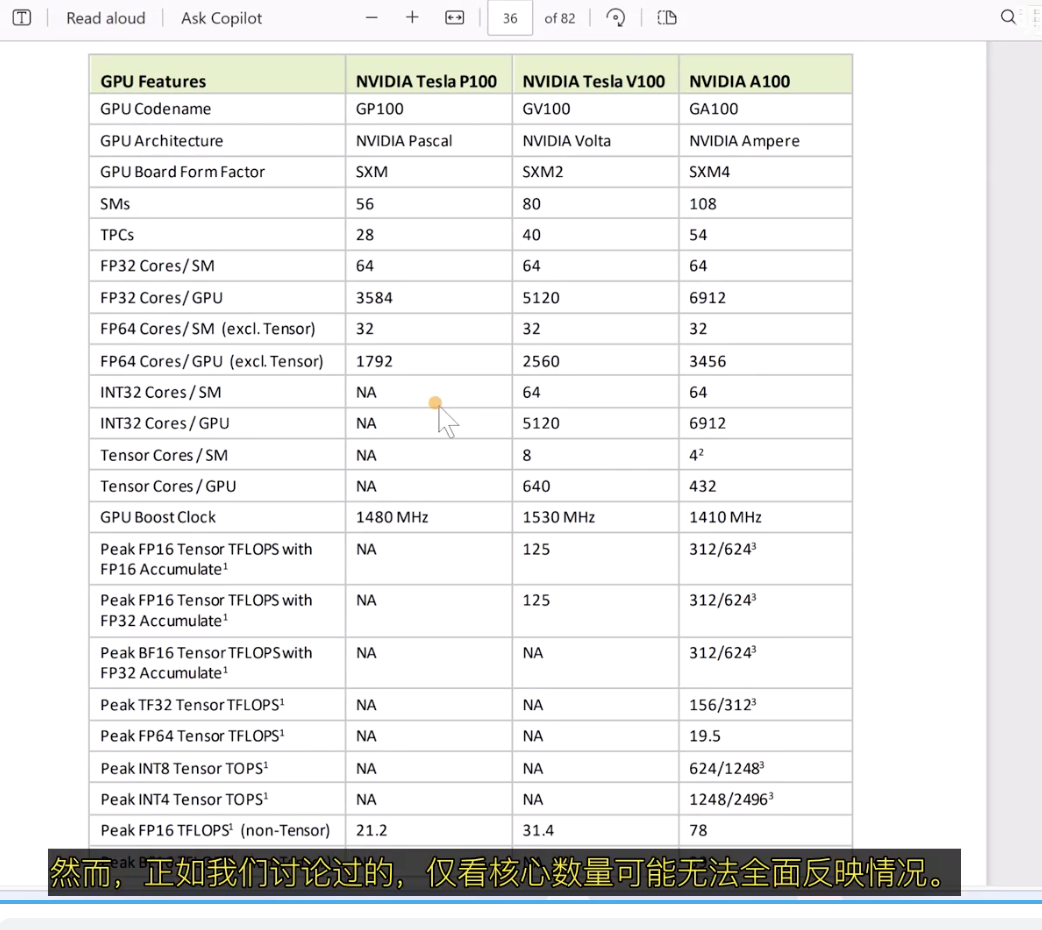
\includegraphics[width=0.75\linewidth]{resources/cuda-035.png}
    \caption{性能数据}
    \label{fig:placeholder}
\end{figure}


\section{半精度、单精度与双精度运算}

大家好，在本文章中我将带大家了解GPU中的不同数据类型和大小。但在这里我想先告诉大家一点，理解数据类型和大小就像在工具箱
中选择合适的工具一样，这是高效且准确完成任务的基础。在GPU计算领域，与CPU类似，我们会根据需求采用不同的方式来存储数
值。例如我们先从整数开始，对于整数我们可以使用八位、16位、32位甚至64位，位数越多能存储的数值就越大。例如一个八位整
数在无符号的情况下可以存储0到255之间的值。如果是有符号变量，则范围为-127到128。

\subsection{整数与浮点类型}

对于64位整数，我们可以存储大得多的数值，最高可达约1800亿亿。这些数字也有不同的大小，当我们处理带小数点的数字时会使
用浮点表示法。例如我们有16位，这被称为半精度。然后是32位，这被称为单精度。最后是64位，这被称为双精度。

在C或 CUDA 编程语言中用int声明变量会使用32位。如果我们将int替换为long，那么通常在内存中会使用64位。
同样的另一方面，如果我们用float声明变量，则在内存中使用32位。但如果将float替换为double，则会在内存中使
用64位。
\subsection{半精度、单精度与双精度的差异}

半精度，它也被称为FP16。这是一种二进制浮点格式，在计算机内存中占用16位，即二个字节。这里的16指的是16位，FP指
的是浮点。半精度提供的数值精度较低，但所需的计算资源更少。

单精度也被称为 FP32。这里的32同样是指存储该类型变量所需的位数，FP指的是浮点。半精度适用于机器学习和图形处理等特
定应用，这些场景通常不需要高精度。这种类型在速度和精度之间取得了折衷，因此单精度成为各类计算任务的首选。

接下来是双精度或称FP64类型。这种类型被视为精度上的强力引擎。这是因为科学计算和复杂仿真中，每一个小数点都可能引发蝴蝶
效应。因此依赖这种类型依赖FP64精度。这种类型确保了对气候模式或分子结构等现象的仿真尽可能接近现实。这种设计及不同的精
度层级，使GPU能够灵活适应各种行业和应用场景。


\begin{figure}
    \centering
    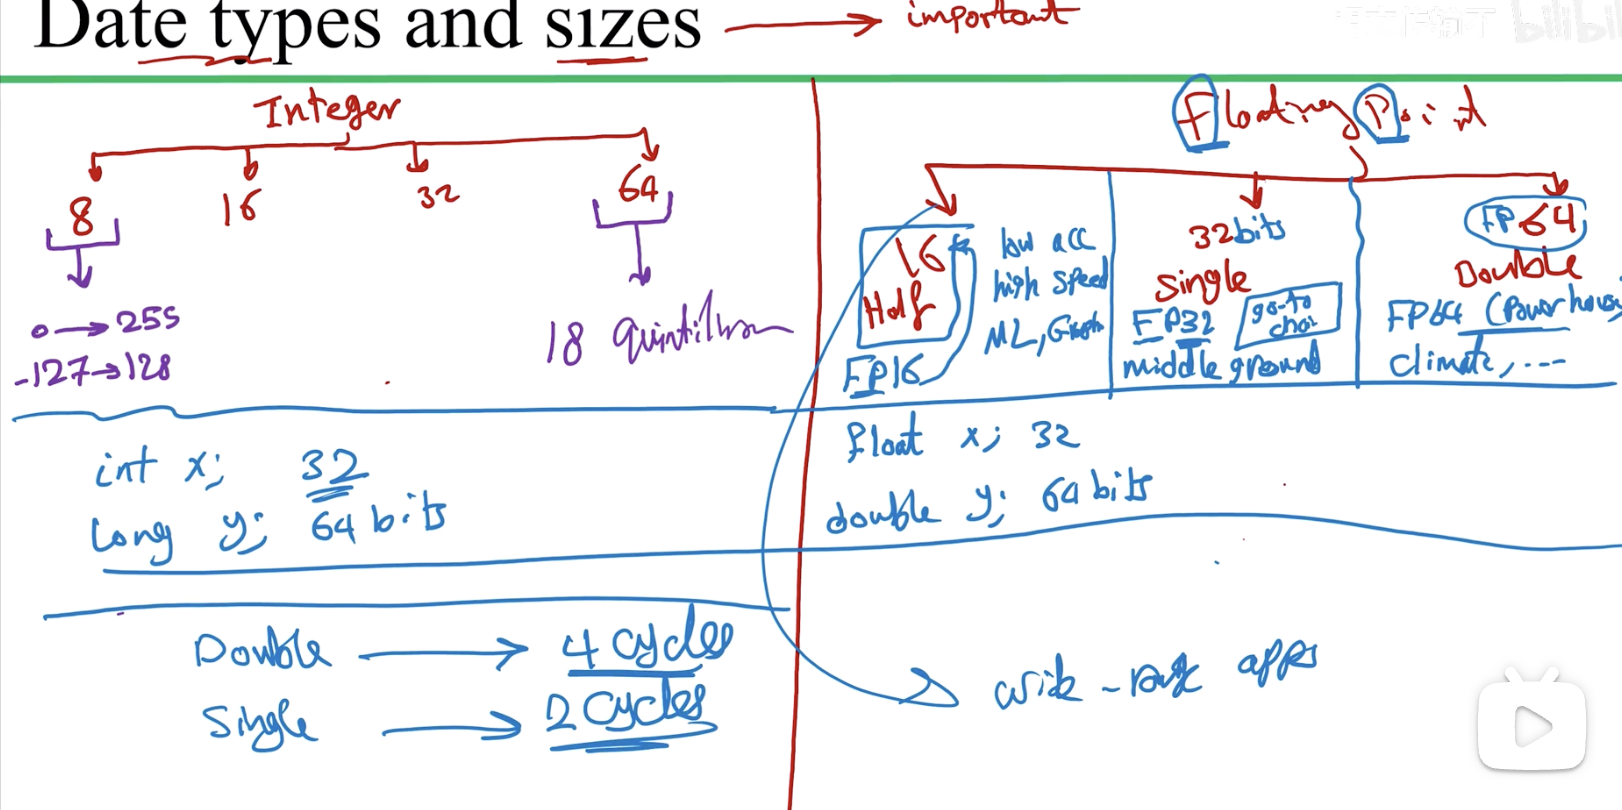
\includegraphics[width=0.75\linewidth]{resources/cuda-036.png}
    \caption{数据类型}
    \label{fig:placeholder}
\end{figure}


\subsection{PI的精度对比}

正因如此，在一篇研究不同GPU数据类型的论文中发现，双精度计算需要四个执行周期。而单精度计算仅需两个周期，这表明双精度虽
然更慢，但提供了更高的精度。例如，如果我们有这里的这段代码，比如floatX，Y和Z我们设X等于10.3。Y等于5.8，
并有一条指令或操作，其中Z等于X加Y那么此操作将仅需两个周期即可完成。然而如果我们将float类型替换为double，同
样的加法操作则需要四个周期才能完成。这种周期数的变化源于双精度数据类型更高的精度和处理需求。

\begin{figure}
    \centering
    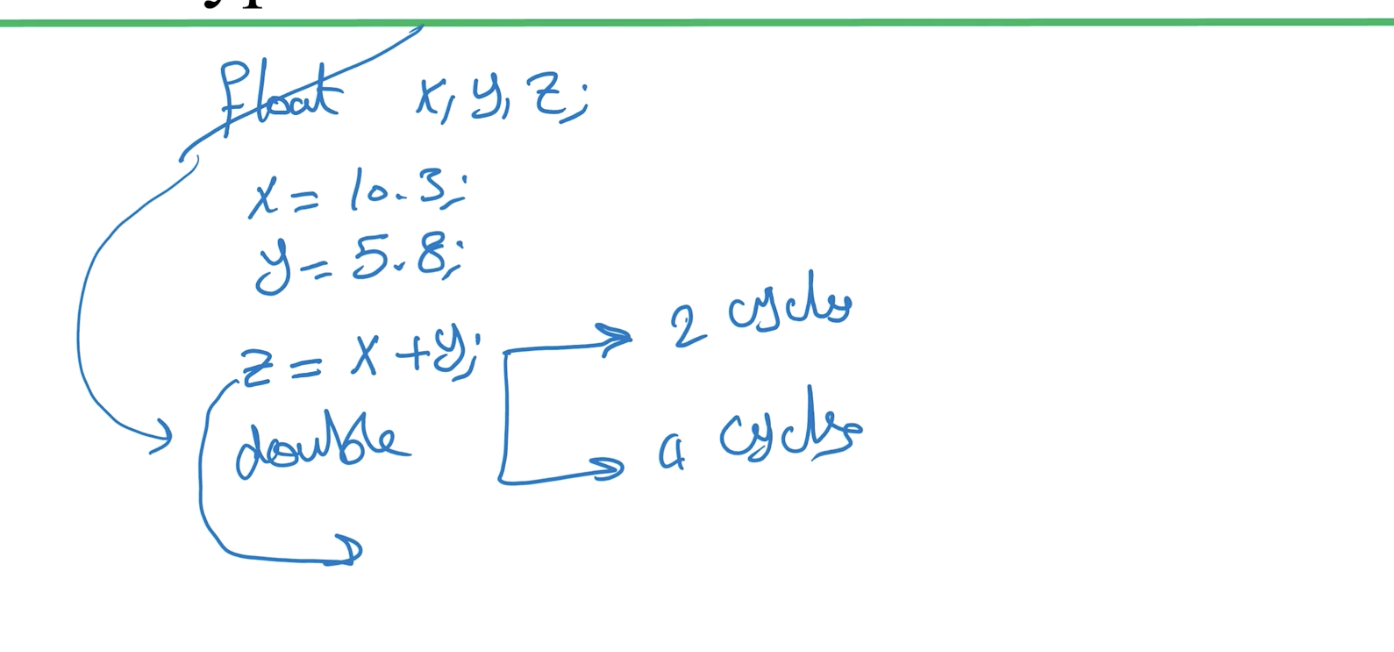
\includegraphics[width=0.75\linewidth]{resources/cuda-037.png}
    \caption{不同计算类型所需时钟周期}
    \label{fig:placeholder}
\end{figure}


为了更清楚的说明，让我们看看圆周率PI在不同浮点精度下的表示方式。在半精度格式中，PI仅保留小数点后两位数字，这意味着像
这样的小数值，正因如此，当需要高精度时会选择双精度。在单精度格式中，这一位数增加到7位，而在双精度格式中进一步扩展到15
位。它实际上会被近似为零。在此处所示的这个数值无法在半精度格式中被准确表示。这一限制是因为半精度最多只支持小数点后2到3
位数字。半精度不适合表示如此精细的数值。

\begin{figure}
    \centering
    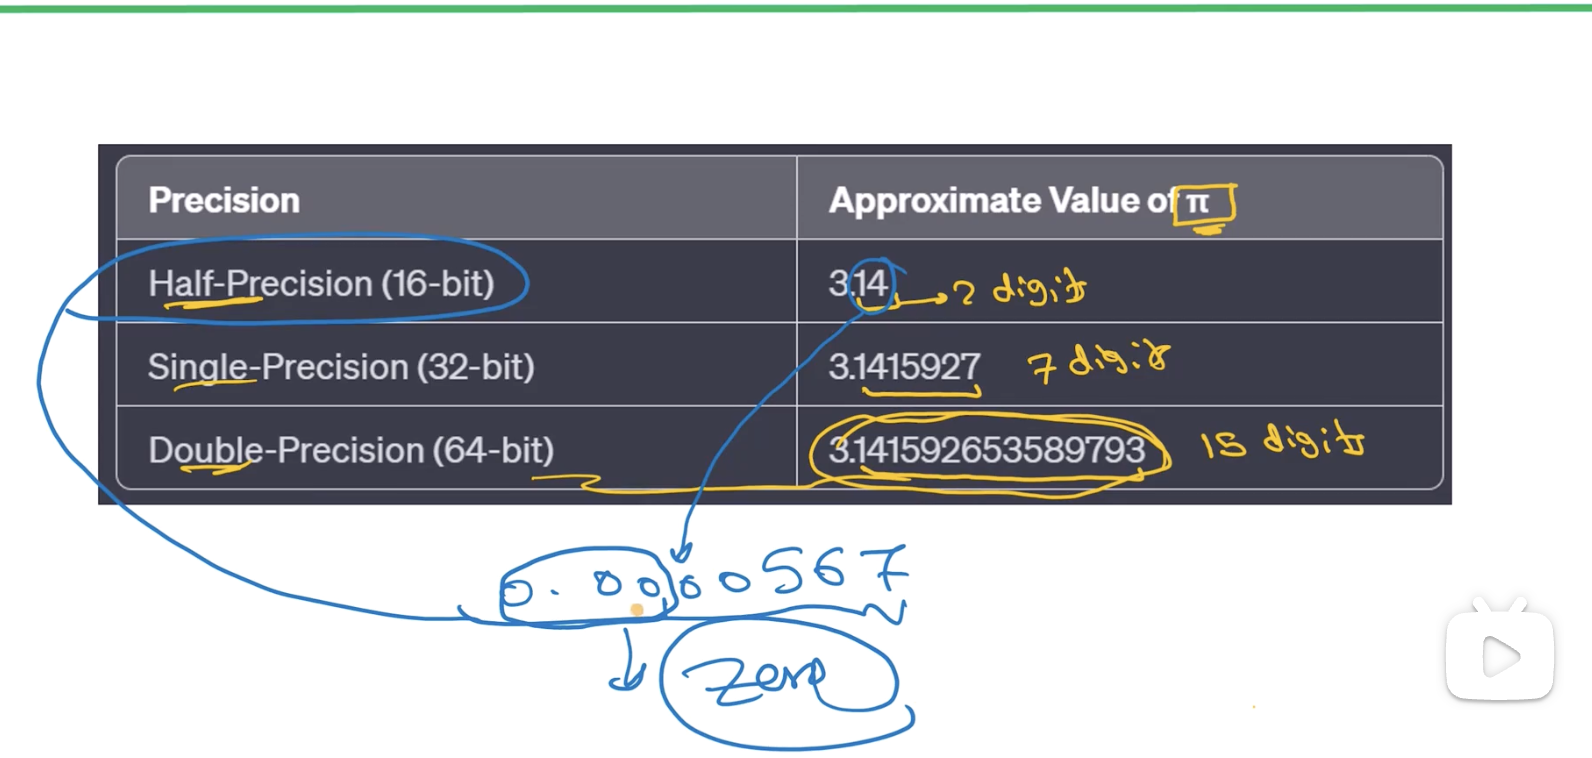
\includegraphics[width=0.75\linewidth]{resources/cuda-038.png}
    \caption{PI的精度}
    \label{fig:placeholder}
\end{figure}


\section{GPU 计算能力}

本章将探讨 GPU 领域中的一个关键术语——计算能力（Compute Capability，简称 CC 编号）。它是 NVIDIA 对 GPU 
架构采用的一种设计分类，表明 GPU 的通用特性和处理能力。为了更深入地理解这一点，我们先从这个问题开始：

计算能力是如何编号或赋予版本号的？

\subsection{计算能力编号}

计算能力以版本号的形式表示，例如 3.0、5.1 或 7.5。小数点前的第一个数字通常表示重大的架构变更，而小数点后的第二个数
字代表较小的改进或扩展。每个版本对应特定一代的 GPU 及其所支持的功能。以 Volta 架构为例，其计算能力被标记为 7。Volta 
因引入了张量核心（Tensor Core）而备受瞩目，大幅提升了特定类型计算的性能，尤其是在人工智能和深度学习领域。这一数字标识
反映了该架构在发布时所引入的一系列前沿特性、能力与改进。

转向 Ampere 架构，其计算能力版本为 8.0。这一提升表明与 Volta 相比，该架构在硬件和软件方面均实现了显著增强：包括更高效
、更强大的张量核心，更大的内存带宽，更高的能效等。这些增强不仅提升了性能，还提高了 GPU 在更广泛应用场景中的效率与通用
性。CC 编号这一概念适用于所有其他架构。

\begin{figure}
    \centering
    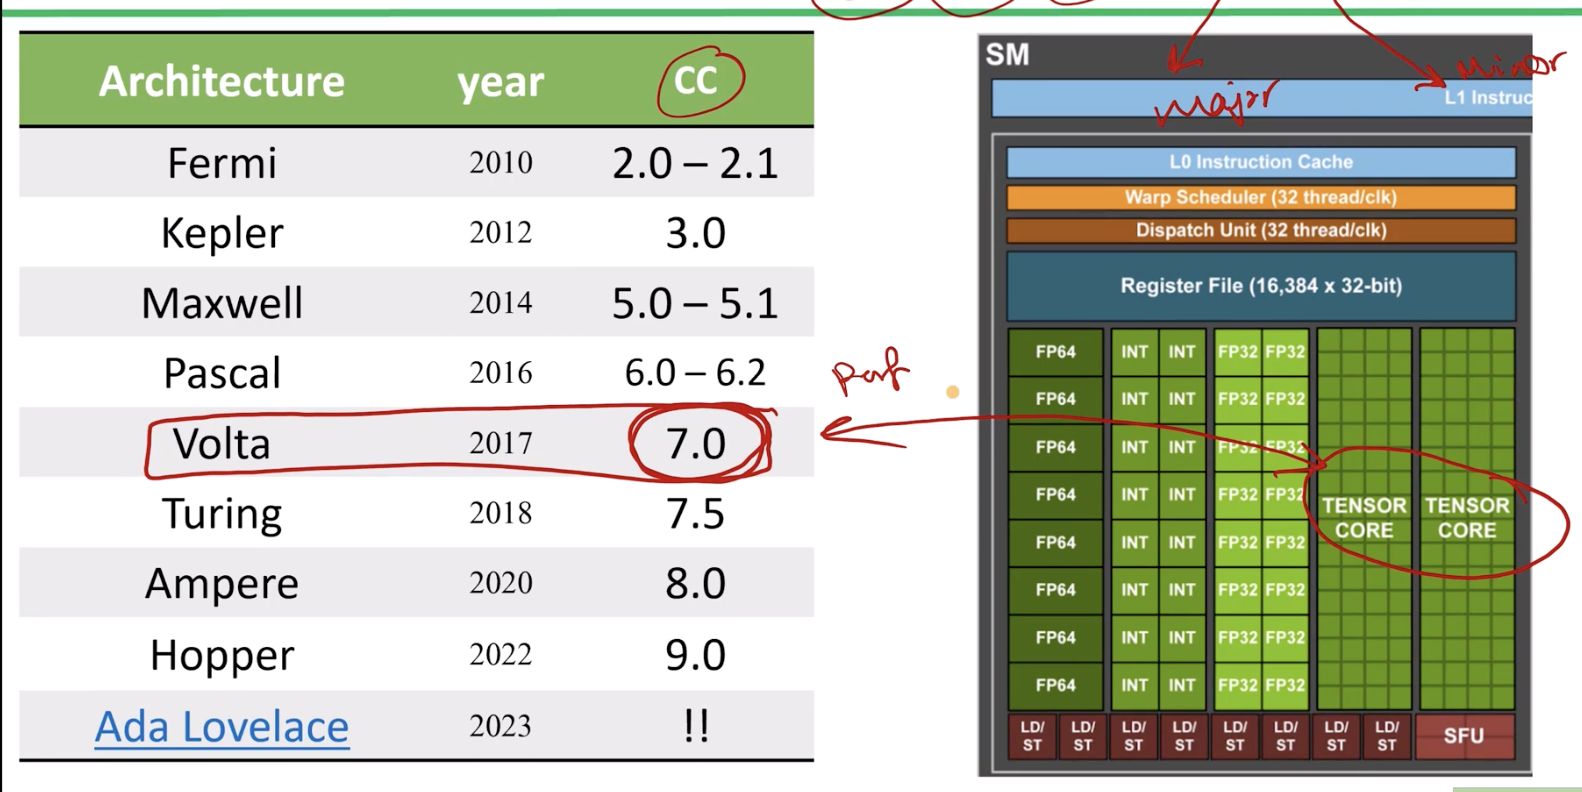
\includegraphics[width=0.75\linewidth]{resources/cuda-039.png}
    \caption{CC版本}
    \label{fig:placeholder}
\end{figure}

\subsection{功能支持}

接下来是本章的第二点——功能支持。不同版本的计算能力支持不同的功能，包括 GPU 能执行的数学运算类型、可处理的并行程度、
内存访问能力等等。例如，当你访问 CUDA 编程文档时会发现许多关于 GPU 编程的章节，其中一节专门介绍计算能力。

\begin{figure}
    \centering
    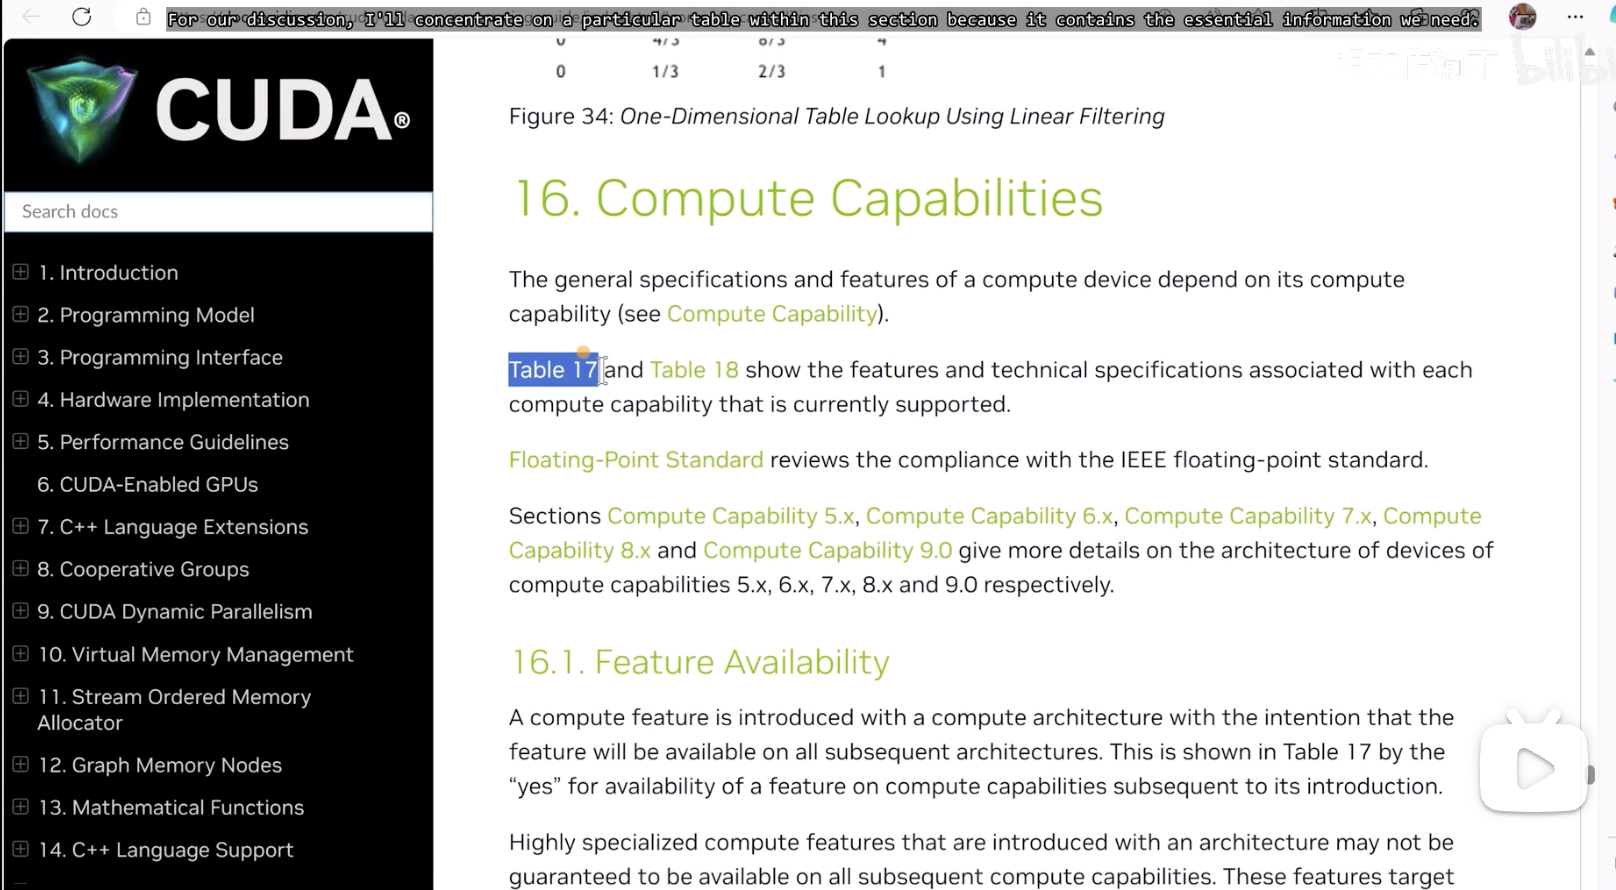
\includegraphics[width=0.75\linewidth]{resources/cuda-040.png}
    \caption{cuda 编程手册}
    \label{fig:placeholder}
\end{figure}


我将聚焦于该节中的一个特定表格，它包含了关键信息。在表 17 中，你可以看到一个结构化的布局——不同计算能力版本列于各列，
对应的功能列于各行。该表格充当对比图表，使开发者能够快速查看特定计算能力的 GPU 支持哪些功能。以计算能力 5.0 为例，从
上到下逐行扫描会发现其中混杂着可用与不可用的功能：具备该计算能力的 GPU 不支持半精度运算，如表所示，在代表计算能力低于
7 的各列中，该项标记为 No。张量核心是另一类重要单元，仅从计算能力 7 及以上版本才开始提供（对应列中标记为 Yes）。表 18 
也体现了相同的概念，留待读者自行查阅。


\subsection{软件兼容性}

更高的计算能力版本能够兼容更新的 CUDA 工具包，而新版本工具包又支持更先进的计算功能和更优的性能优化。换言之，GPU 的计算
能力决定了它可运行的 CUDA 工具包的版本。为了说明这一概念，以 PTX 兼容性为例——为简化理解，可将 PTX 视作一种 GPU 汇编
语言。部分 PTX 指令只能在特定计算能力版本的设备上执行，因为它们依赖于仅存在于特定计算能力 GPU 上的硬件单元或功能。

\begin{figure}
    \centering
    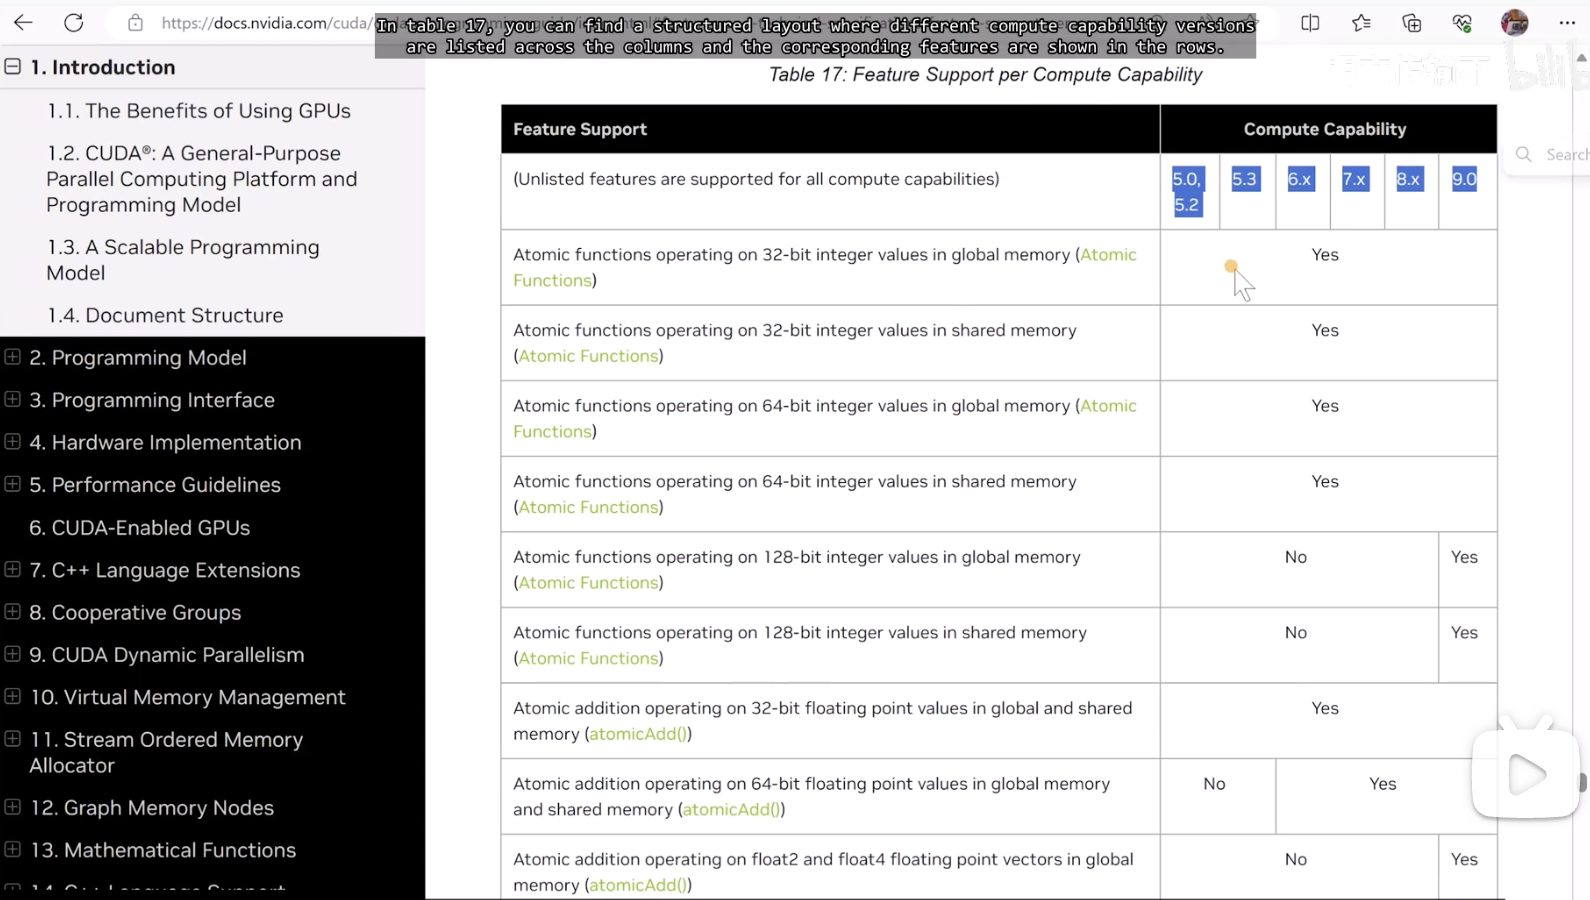
\includegraphics[width=0.75\linewidth]{resources/cuda-041.png}
    \caption{cuda 编程手册}
    \label{fig:placeholder}
\end{figure}


\begin{figure}
    \centering
    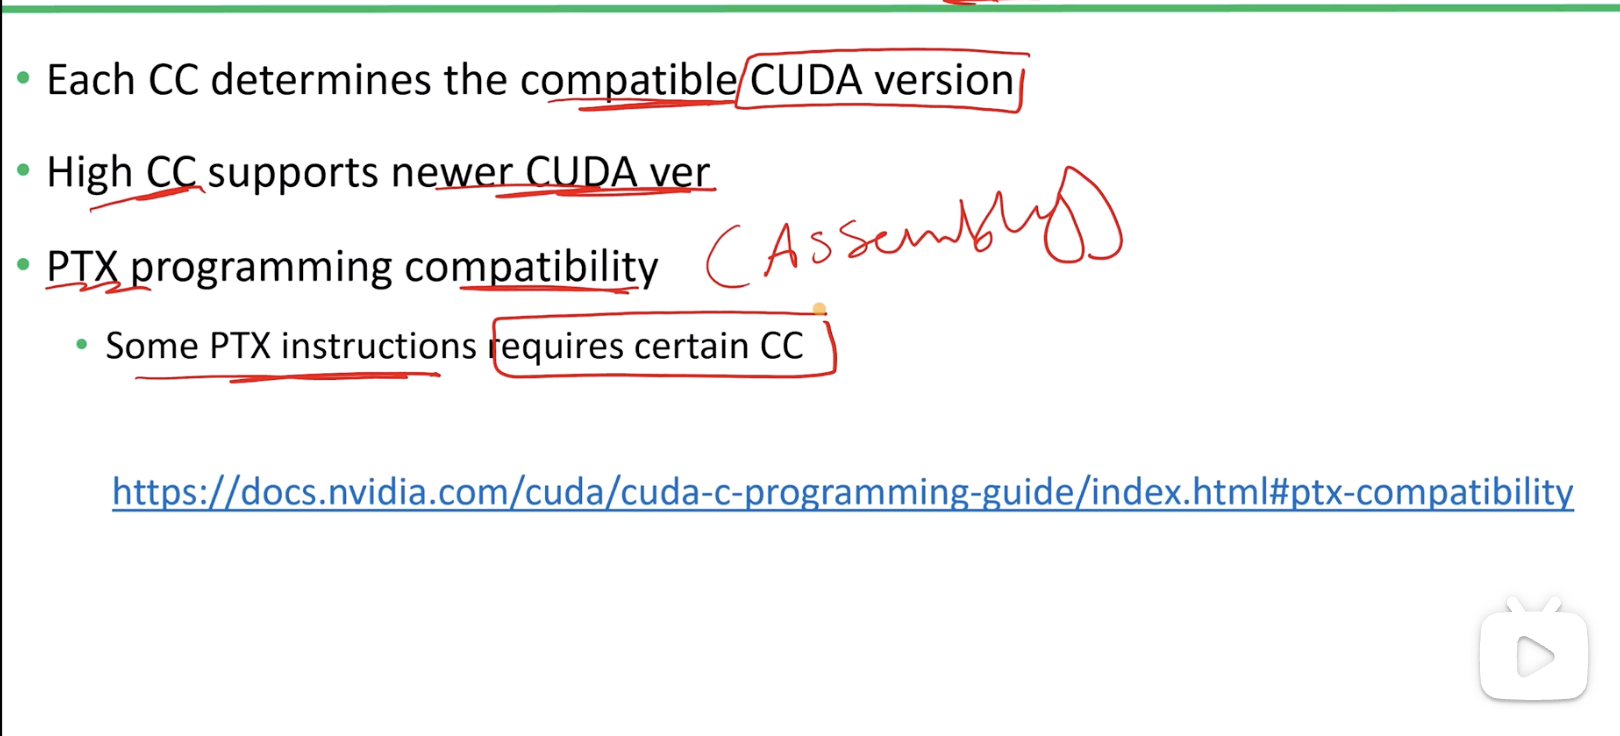
\includegraphics[width=0.75\linewidth]{resources/cuda-042.png}
    \caption{cuda 编程手册}
    \label{fig:placeholder}
\end{figure}


通过链接进入 \href{https://docs.nvidia.com/cuda/cuda-programming-guide/index.html}{CUDA C 编程指南}，你会发现
文档明确指出了某些 PTX 指令对计算能力的版本要求，这些操作或函数仅在计算能力高于 5 的设备上可用。例如 Warp Shuffle 函数
，它能在 Warp 内的线程之间共享数据，而无需使用共享内存或全局内存。

\begin{figure}
    \centering
    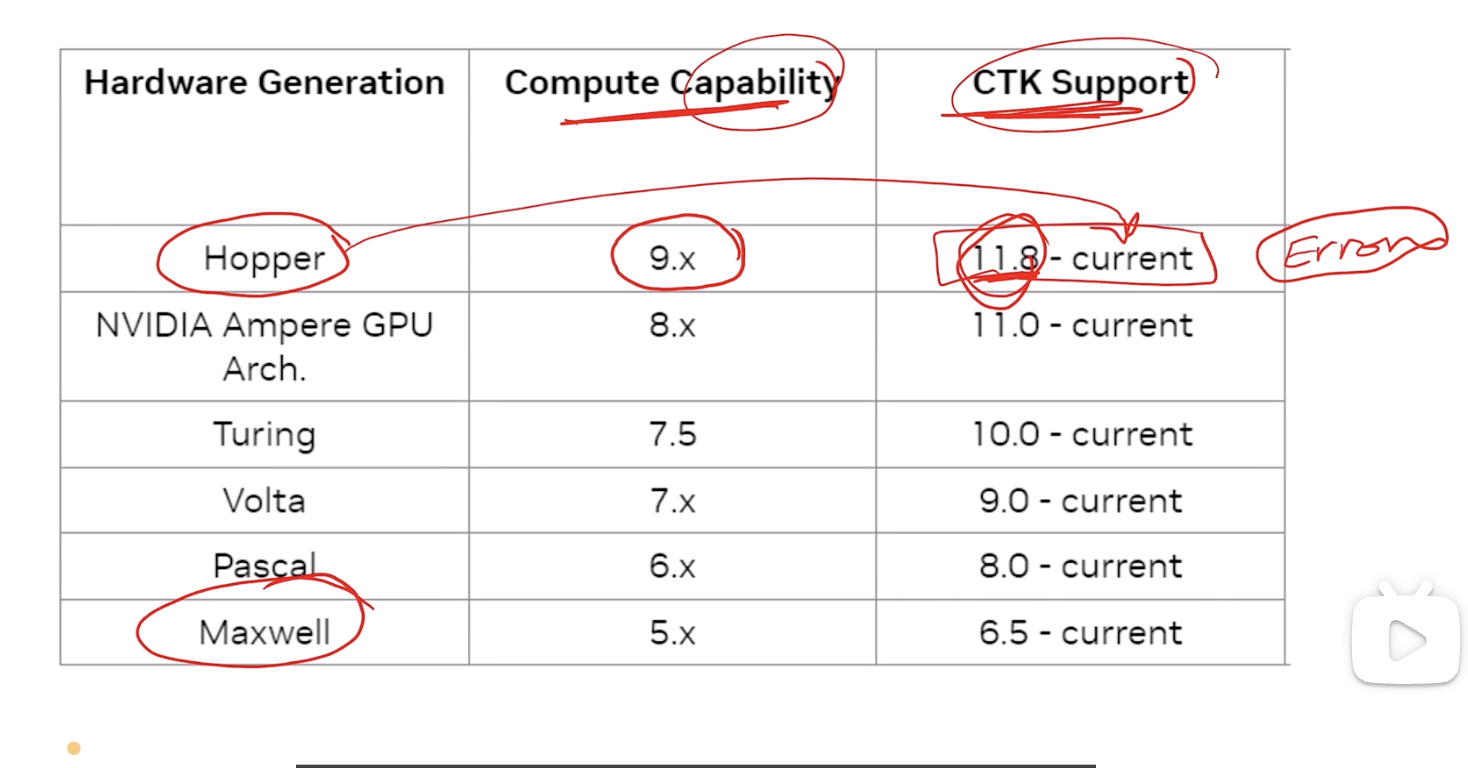
\includegraphics[width=0.75\linewidth]{resources/cuda-043.png}
    \caption{cuda 版本}
    \label{fig:placeholder}
\end{figure}

如果还不够清楚，我们再来看另一个例子。假设你正在从事一个需要最新机器学习技术的项目，你的 GPU 的计算能力将决定你能否使用
最新的 CUDA 工具包——该工具包包含最新的功能和性能优化，可能正是你的应用所需的。

再比如说，如果你使用的是 Hopper 架构的 GPU（目前全球最新一代 GPU 之一），那么对应的计算能力为 9.x。如本表所示，这不仅仅是
对前几代产品的小幅升级，意味着 Hopper GPU 已准备好处理最先进的计算任务。它对 CUDA 工具包的最低版本要求为 11.8，因此在
Hopper 架构中无法使用低于 11.8 的 CUDA 版本。类似地，Maxwell 架构的计算能力编号为 5.x，其最低 CUDA 工具包版本要求为
6.5——如果版本不兼容，你会收到错误提示。

如本表所示，计算能力与所支持的 CUDA 版本之间的关系是理解如何使硬件选择与软件需求相匹配的关键。无论你是开发者、研究人
员，还是依赖 GPU 进行高强度任务的用户，了解这一关系都有助于确保项目运行顺畅、高效并避免意外问题。最后，你可以在此处展
示的网页上发现专为不同应用场景设计的各类 GPU，每一款 GPU 都附带其对应的计算能力，详情见各表格。


\section{如何阅读 GPU 技术白皮书}

欢迎各位。今天，我们将探索图形处理器白皮书的奇妙世界。白皮书本质上是图形处理器架构的数据表或深入技术规格说明书。这些文档
即白皮书，在比较不同图形处理器时具有无可估量的价值，因为他们提供了对每个架构规格和能力的详细洞察。回到这里的表格，你会注
意到针对每个架构，我们都有一个基于该架构的芯片示例。

\begin{figure}
    \centering
    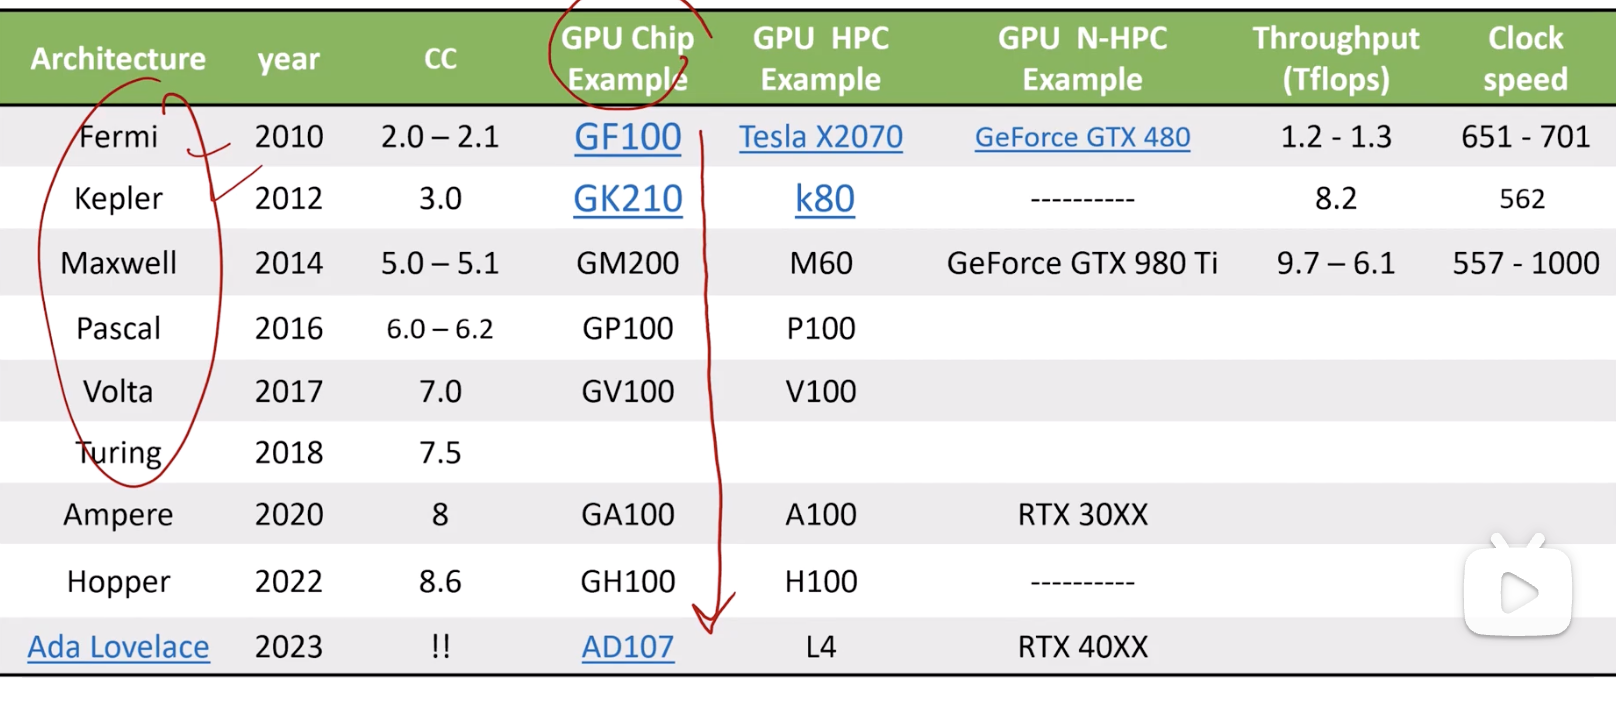
\includegraphics[width=0.75\linewidth]{resources/cuda-044.png}
    \caption{GPU 架构}
    \label{fig:placeholder}
\end{figure}

\subsection{搜索白皮书}

要获取任何架构的白皮书，只需要一次简单的互联网搜索。只需打开你的浏览器，输入芯片名称后加上白皮书一词，而芯片名称可以从这
个表格中过去。这很简单，一旦你这样做了，你很可能就能找到你想要的东西。你可以搜索表格中的芯片名称GF100，然后加上白皮
书。完成这一步后，点击回车，你将看到一系列搜索结果。

\begin{figure}
    \centering
    
\includegraphics[width=0.75\linewidth]{resources/cuda-045.png}
    \caption{搜索白皮书}
    \label{fig:placeholder}
\end{figure}


你需要寻找那个代表官方白皮书的PDF文件。正如你所见，我们找到了GF100芯片的白皮书。请记住，你寻找的链接应该指向一份
包含完整技术规格的PDF文档。同样地，如果你在研究安培架构，你会搜索GA100白皮书。因为有时你可能会偶然看到文章或总结
，但你真正想要的是原始的全篇白皮书。如你所见，我们拿到了GA100芯片白皮书的PDF文件，让我带你在本文章中了解另一个要
点。英伟达有一个很有帮助的做法，就是在其白皮书中将新架构与旧架构进行比较，以及Pascal架构即V100和P100的性能
比较。如果你正在阅读A100图形处理器或GA100芯片或Ampere 架构的白皮书，你很可能会发现他与前任架构。


\begin{figure}
    \centering
    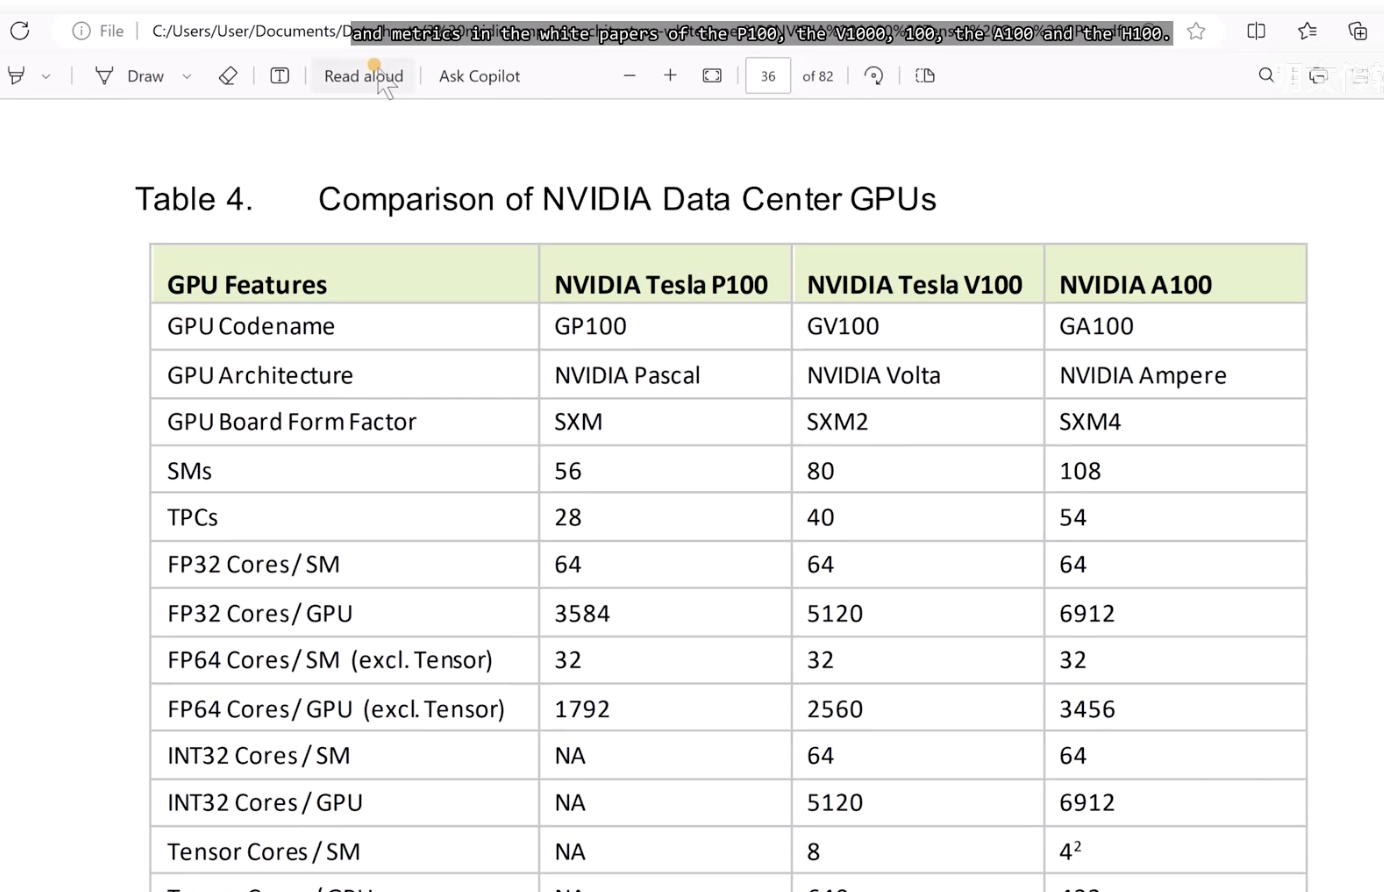
\includegraphics[width=0.75\linewidth]{resources/cuda-046.png}
    \caption{架构比较}
    \label{fig:placeholder}
\end{figure}

例如，你可能会在P100、V100。这就是为什么我们观察到一个有趣的现象，即某些表格和图表可以在不同的白皮书中找到。
A100和H100的白皮书中看到展示不同单元和指标的同一个表格。但我告诉你，正如你现在所见，所有白皮书中的这种一致性意味着一
旦你理解了如何浏览并解读一份英伟达白皮书，那么你就具备了理解其他白皮书的能力。

\subsection{白皮书的结构}

这还不止于此，英伟达的白皮书通常遵循标准化的结构，按顺序包含以下要点，第二点是流式多处理器的内部组件和结构。第一点是新特
性的介绍，第三点是性能基准测试与比较，最后一点是技术规格。让我们从第一点开始，新特性的介绍。每份白皮书都以一个突出展示新
技术和增强功能的部分开始。这可以是任何内容从用于人工智能计算的新型核心，如张量核心，到改进的图形着色技术，甚至是软件或硬
件的任何增强。

\begin{figure}
    \centering
    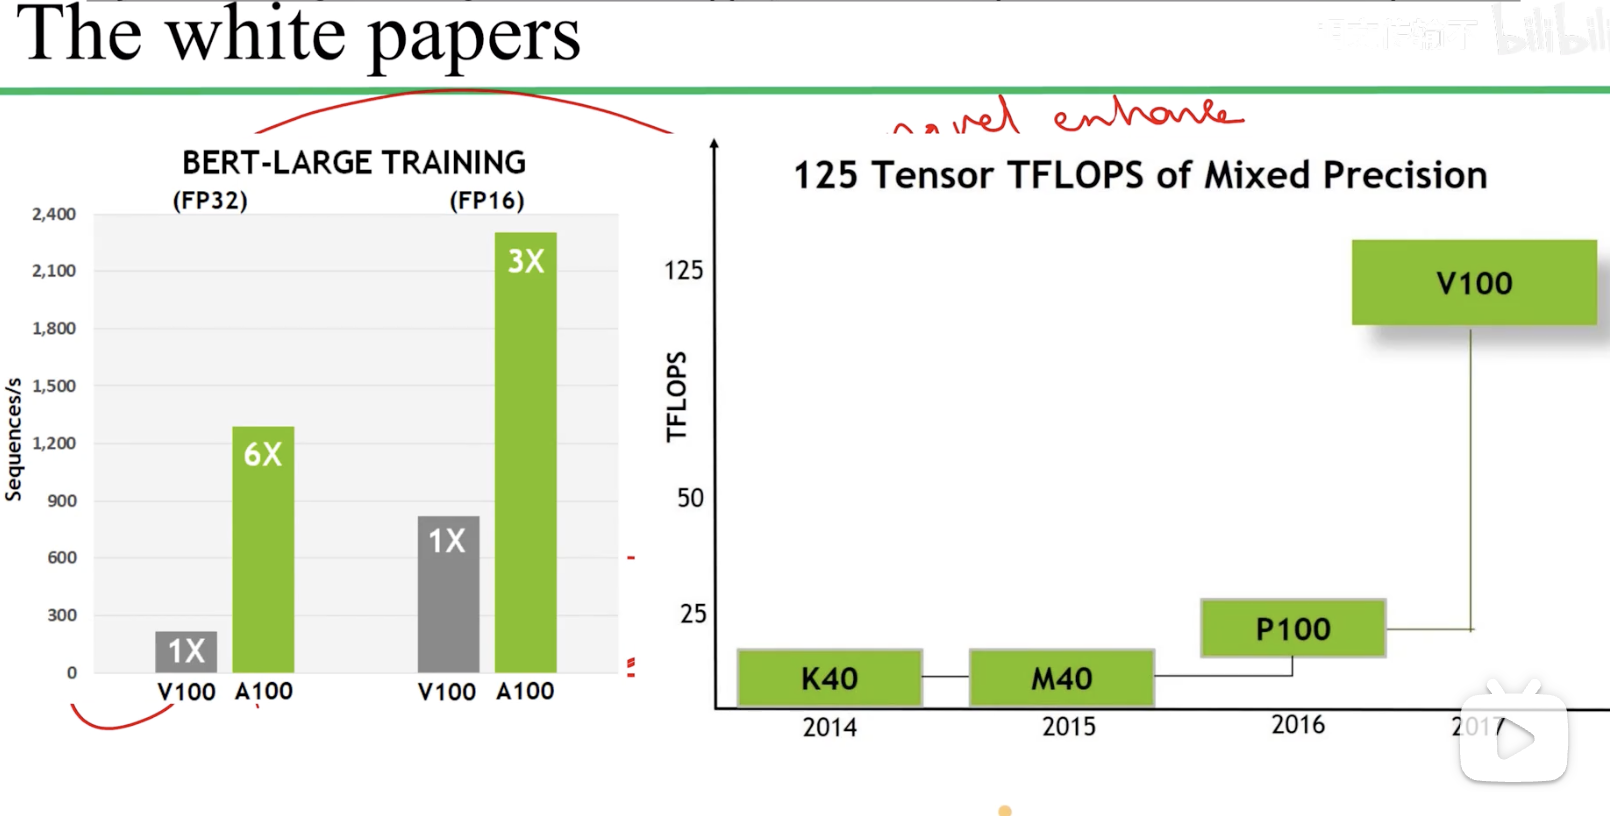
\includegraphics[width=0.75\linewidth]{resources/cuda-047.png}
    \caption{架构比较}
    \label{fig:placeholder}
\end{figure}


第二点是流式多处理器的内部结构或组件。然后是性能基准测试比较。所有白皮书都会深入探讨新型流式多处理器的架构。正如你在我从
不同白皮书中拿来的这些图片中所见，每个架构与其前任都有不同的比较。最后是技术规格，这就是你在每份白皮书中将找到的四个主要
要点。在所有白皮书中都包含详细规格，如核心数量、内存大小、内存带宽、内存技术、功耗要求，以全面展示图形处理器的能力。

\subsection{SM内部结构}

我们将重点关注第二点，计流式多处理器的内部结构。从流式多处理器的内部结构或内部组件开始，英伟达的白皮书深入剖析了每个图形
处理器的流式多处理器设计。接着是我们已经讨论过的通用对比表。例如如果你查看基于Pascal架构的P100图形处理器的白皮
书，即GA100芯片的白皮书，你会注意到这里有一张展示整个图形处理器的图片，然后是流式多处理器的详细图表及其内部组件，如
CUDA核心和内存层级的描述层级。例如我们这里有整个图形处理器，然后有对比表，当我们转向V100白皮书或福特架构白皮书时
会发现类似的布局。最后是流式多处理器的内部结构或内部组件。然而在这里你会观察到一个显著的增强，既增加了张量核心单元。正如
你在这里看到的，Volta架构中有了张量核心单元，但在 Pascal 架构中则没有这样的单元。

让我们继续看A100白皮书或 Ampere架构白皮书。同样这份白皮书展示了整个图形处理器，然后我们看到了流式多处理器内部
结构的详细信息。但我们没有对比表，因为他们把对比表移到了另一个部分。但无论如何，我们在白皮书中还是能看到它。然后正如你所
见，Ampere架构的布局可能看起来有些熟悉，因为它与福特架构中流式多处理器的内部结构非常相似。只要看看这里的这两张图片
，你就会发现没有巨大的变化。

当我们查看H100白皮书或Hopper白皮书时，这种一致性依然存在。然后这个图形处理器架构后面跟着流式多处理器内部结构的
详细信息，这份白皮书呈现了整个图形处理器，正如你在这里看到的，如你所见，这个架构与所有前任架构的主要区别在于每个流式多处
理器中可用的核心数量。例如，你可以数一下在这个架构中有多少个32位浮点核心。并将其与比方说A100图形处理器进行比较，看
看差异。

\begin{figure}
    \centering
    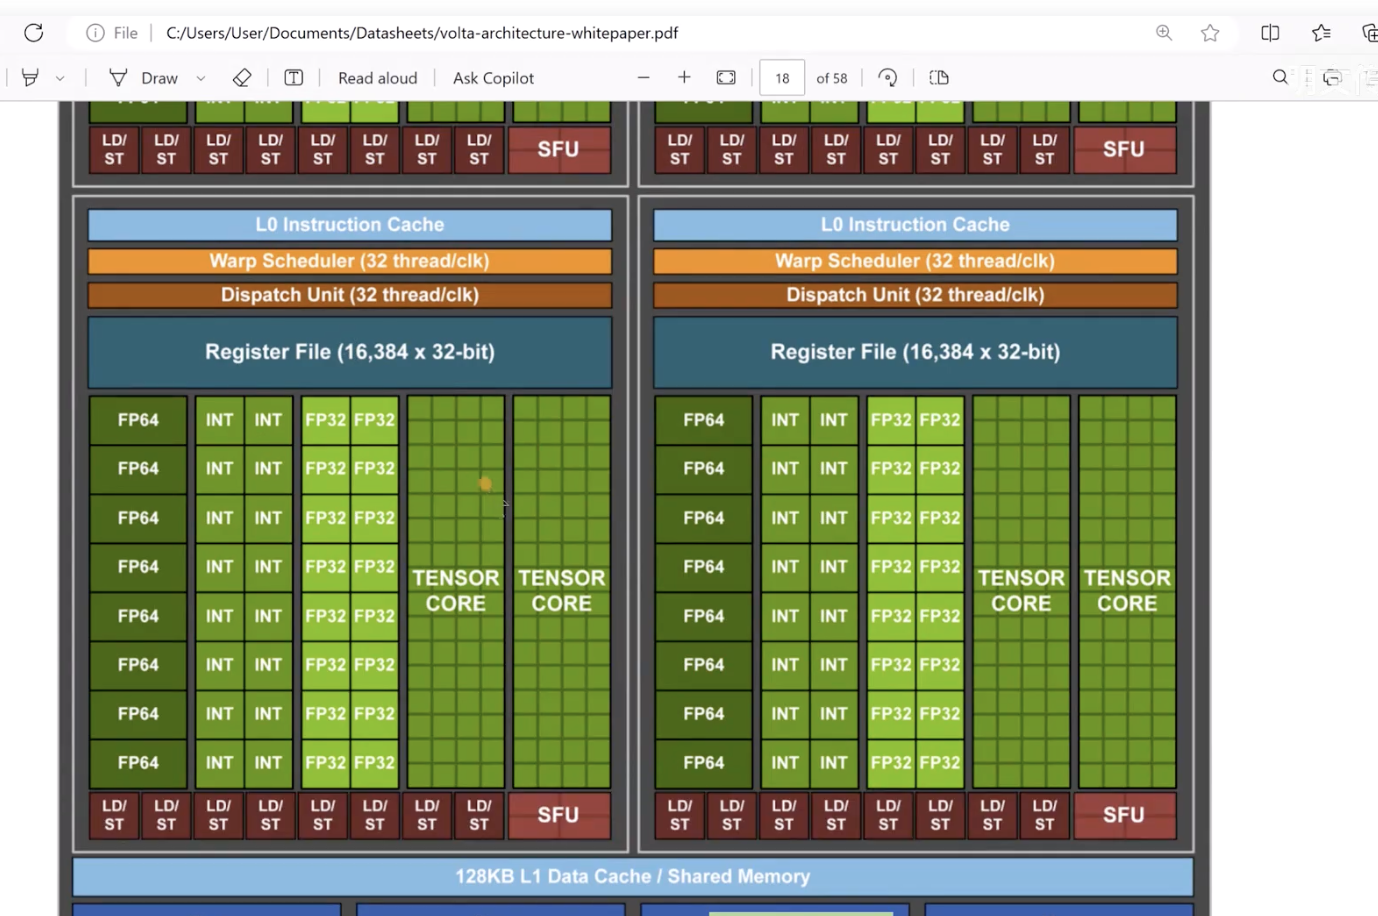
\includegraphics[width=0.75\linewidth]{resources/cuda-048.png}
    \caption{Volta 架构}
    \label{fig:placeholder}
\end{figure}

现在总结一下，我想说的是，虽然每份白皮书都针对其特定的图形处理器，但所有白皮书提供的结构和信息类型都遵循相似的模式。这种
延续性和一致性不仅使专业人员更容易跟上最新技术。而且有助于清晰的理解技术的进步，以及每个新架构与其前任相比的定位。


\section{Volta 架构白皮书阅读}

前几章中，我们已详细探讨了英伟达白皮书中常见的关键参数。在深入探讨 Volta 架构之前，回顾前几章的内容非常重要——它们
奠定了理解本章主题所必需的基础知识。熟悉这些参数至关重要，因为我们将在本章中引用并验证它们。

现在就来看看 Volta 架构的规格。打开 Volta 白皮书（即 V100 白皮书），你可以在开头看到目录。在目录的第二页，你会找到一
个名为"关键特性"的部分。这不仅仅是一系列改进的列表，更是 V100 相比前代架构重大增强的全面概述。

点击"关键特性"标题后，我们将看到定义 V100 GPU 即 Volta 架构的核心特性，从新的 SM 设计到第二代 NVLink 技术等。
本章将逐一讨论所有这些增强功能。回到目录，这份白皮书的一个突出方面是专门聚焦于人工智能和深度学习。考虑到 Volta 架构首
次引入了张量核心（Tensor Core），这种对 AI 和深度学习的聚焦是十分自然的。

\begin{figure}
    \centering
    
\includegraphics[width=0.75\linewidth]{resources/cuda-049.png}
    \caption{Volta 架构关键特性}
    \label{fig:placeholder}
\end{figure}

\begin{figure}
    \centering
    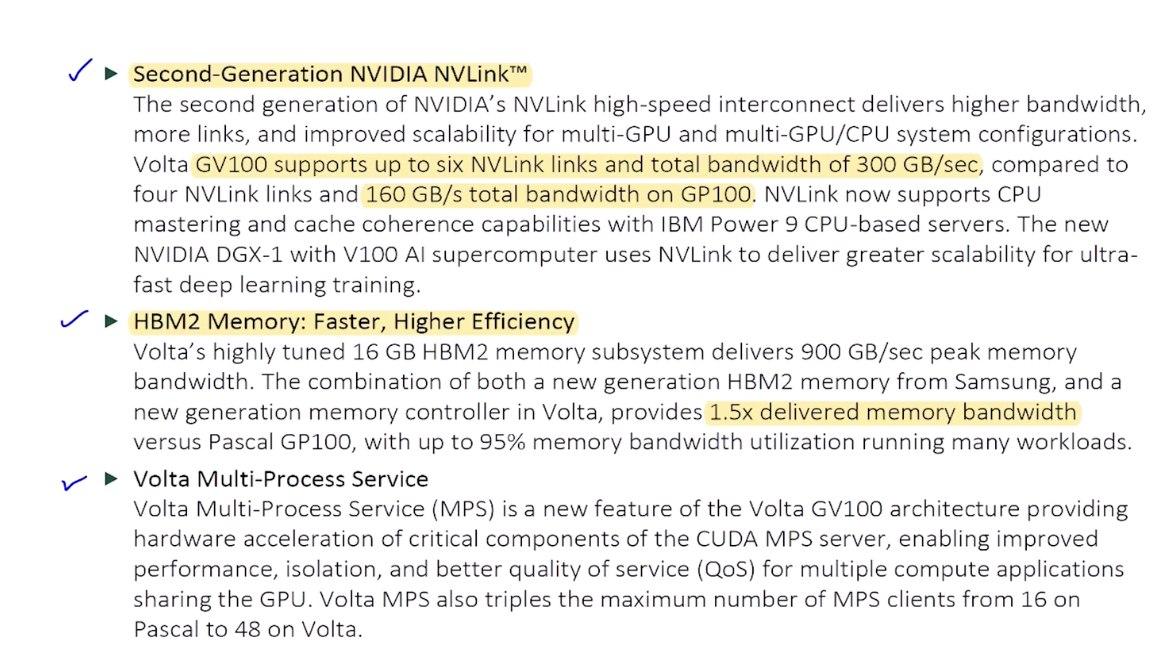
\includegraphics[width=0.75\linewidth]{resources/cuda-050.png}
    \caption{Volta 架构关键特性}
    \label{fig:placeholder}
\end{figure}


\subsection{Volta关键特性}

张量核心是专门设计用来执行矩阵运算的计算单元，这对神经网络的训练和推理阶段至关重要，也是 Volta 架构的重大突破。请注
意目录中“深入硬件架构”这个关键标题。这一标题并非 Volta白皮书独有，它在英伟达各款白皮书中反复出现。例如，Pascal 白皮书和最近的 Hopper (H100)白皮书目录中都有相同的术语。
这提醒了我们之前讨论过的重要一点：尽管每份白皮书详述不同的架构，但英伟达白皮书采用了相似的结构方法。此外，Volta白皮书还包含软件增强部分以及提供其他设备详细信息的附录。

现在，让我们深入浏览白皮书。文中提到 V100 GPU 拥有约 210 亿个晶体管。作为对比，H100 包含 800亿个
晶体管。这意味着从 Volta 到 Hopper，晶体管数量增加了近 4 倍。晶体管数量是可用的计算资源指标，更多的晶体管
通常对应硬件单元数量的增加。

\subsection{SM增强}

接下来讨论 Volta 架构的关键特性和增强。首先是 \textbf{SM 增强}：


\begin{figure}
    \centering
    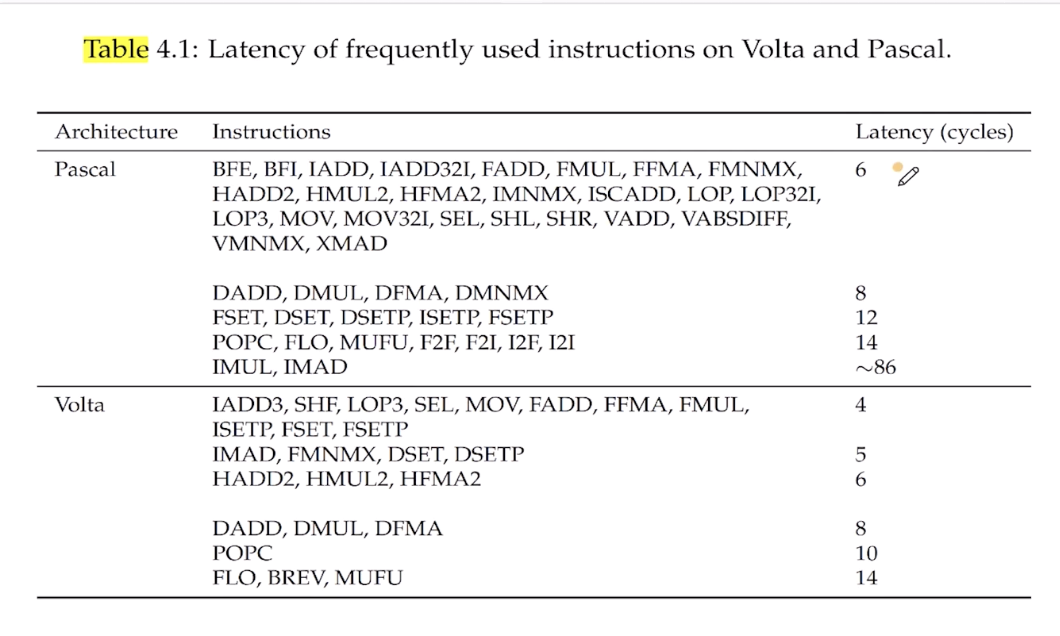
\includegraphics[width=0.75\linewidth]{resources/cuda-051.png}
    \caption{Volta 单精度和双精度核心改进}
    \label{fig:placeholder}
\end{figure}


\begin{enumerate}
    \item \textbf{能效提升}：Volta 的新 SM 设计比前代 Pascal 架构能效高出 50\%。对于管理大规模计算系统的企业来说，这意味着 V100 有可能将能源成本减半，且不牺牲计算能力。

    \item \textbf{单精度和双精度核心改进}：在功耗不变的情况下，新 SM 为 FP32（单精度）和 FP64（双精度）性能提供了重大改进。研究论文中的指令延迟对比表显示，Pascal 中加法/减法指令需要 6 个周期，而 Volta 仅需 4 个周期。后续的 Ampere 架构进一步降至 2 个周期。这说明英伟达不仅增加了核心数量，也在不断提升现有单元的执行速度。

    \item \textbf{用于 AI 计算的张量核心}：这是新 SM 中的全新单元，能为神经网络训练带来高达 12 倍的吞吐量提升（TFLOPS），推理方面提升 6 倍。虽然张量核心的单条指令延迟在 4-8 个周期之间（取决于矩阵形状和数据类型），但它们是在矩阵级别而非单个元素上执行操作，从而实现了巨大的性能飞跃。

    \item \textbf{增强的整数和浮点数并行性}：在 Pascal 及更早架构中，整数和浮点运算无法同时执行。但在 Volta 的新 SM 中，每种运算都有独立路径，允许整数和浮点运算并行运行。这对于混合数据类型的现代工作负载至关重要。

    \item \textbf{高级线程调度与内存合并}：除了提升访问速度外，还将 L1 高速缓存和共享内存合并到了一个物理单元中。
\end{enumerate}

第二个架构级增强是\textbf{第二代 NVLink 技术}（稍后详述）。

第三个特性是\textbf{全局内存增强}。Volta 的内存带宽达到 900\,GB/s，而 Pascal 约为700 \,GB/s。相比之下，Ampere 架构达到了约1500\,GB/s。更高的内存带宽意味着更快的数据访问和更高的数
据处理效率。

\begin{figure}
    \centering
    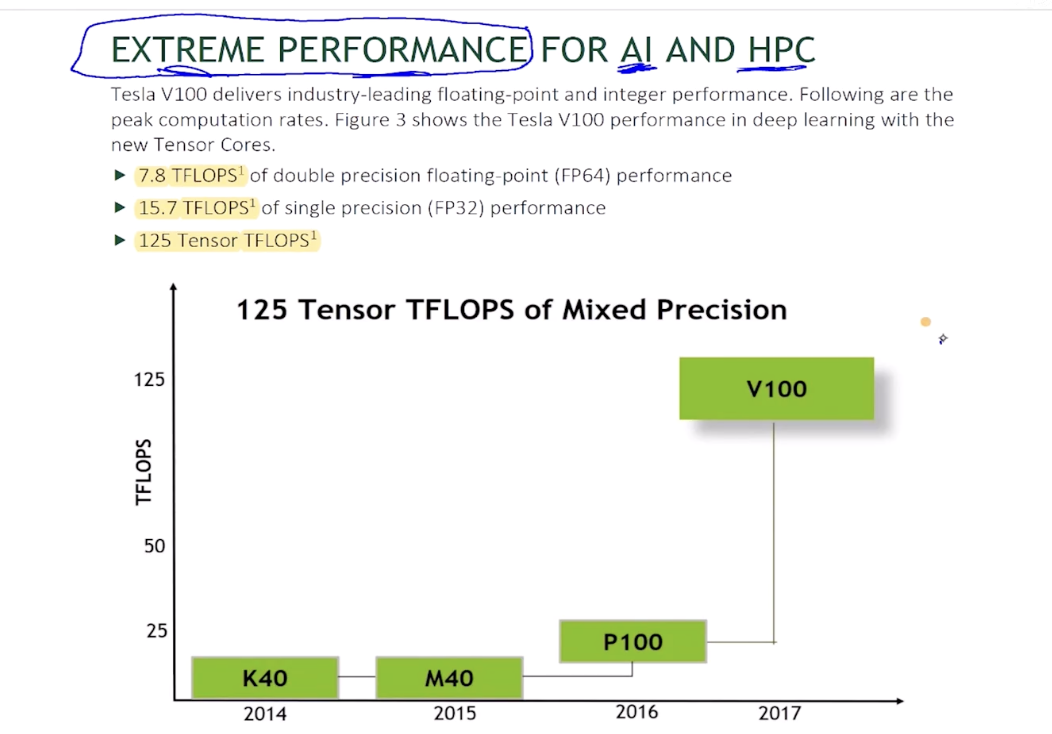
\includegraphics[width=0.75\linewidth]{resources/cuda-052.png}
    \caption{Volta 性能提升}
    \label{fig:placeholder}
\end{figure}


此外，还有\textbf{多进程服务（MPS）}，旨在优化单个 GPU上同时执行的多个应用程序的性能；以
及\textbf{统一内存}增强，将 GPU 和 CPU内存合并为单一虚拟地址空间。最后，常用的 GPU 加速计算库也进
行了更新，以有效利用这些新硬件单元。

白皮书强调了针对 AI 和高性能计算的“极致性能”。引入张量核心后，V100 实现了 125\,TFLOPS的吞吐量，相
比 Pascal 的约 21\,TFLOPS 是显著提升。

\subsection{深入硬件架构}

接下来进入最重要的部分：\textbf{深入探讨 GV100 GPU 硬件架构}。每个 GPU 包含多个 SM，每个SM
包含 L1/共享内存及各类计算单元。在 Volta 中，每个 SM 配备 64 个单精度核心、64个整数核心、32 个双
精度核心和 8 个张量核心。整个 GPU 拥有 84 个 SM，总计约有 2 万个计算单元。GPU内部还包括 6\,MB
的二级高速缓存（L2 Cache），通过内存控制器连接所有 SM，底部则是用于互联的NVLink 单元。

深入单个 SM，它由\textbf{四个分区}组成。这种分区策略允许将不同的软件块分配到不同分区并发执行，最大化资源利用
率。每个分区包含：

\begin{figure}
    \centering
    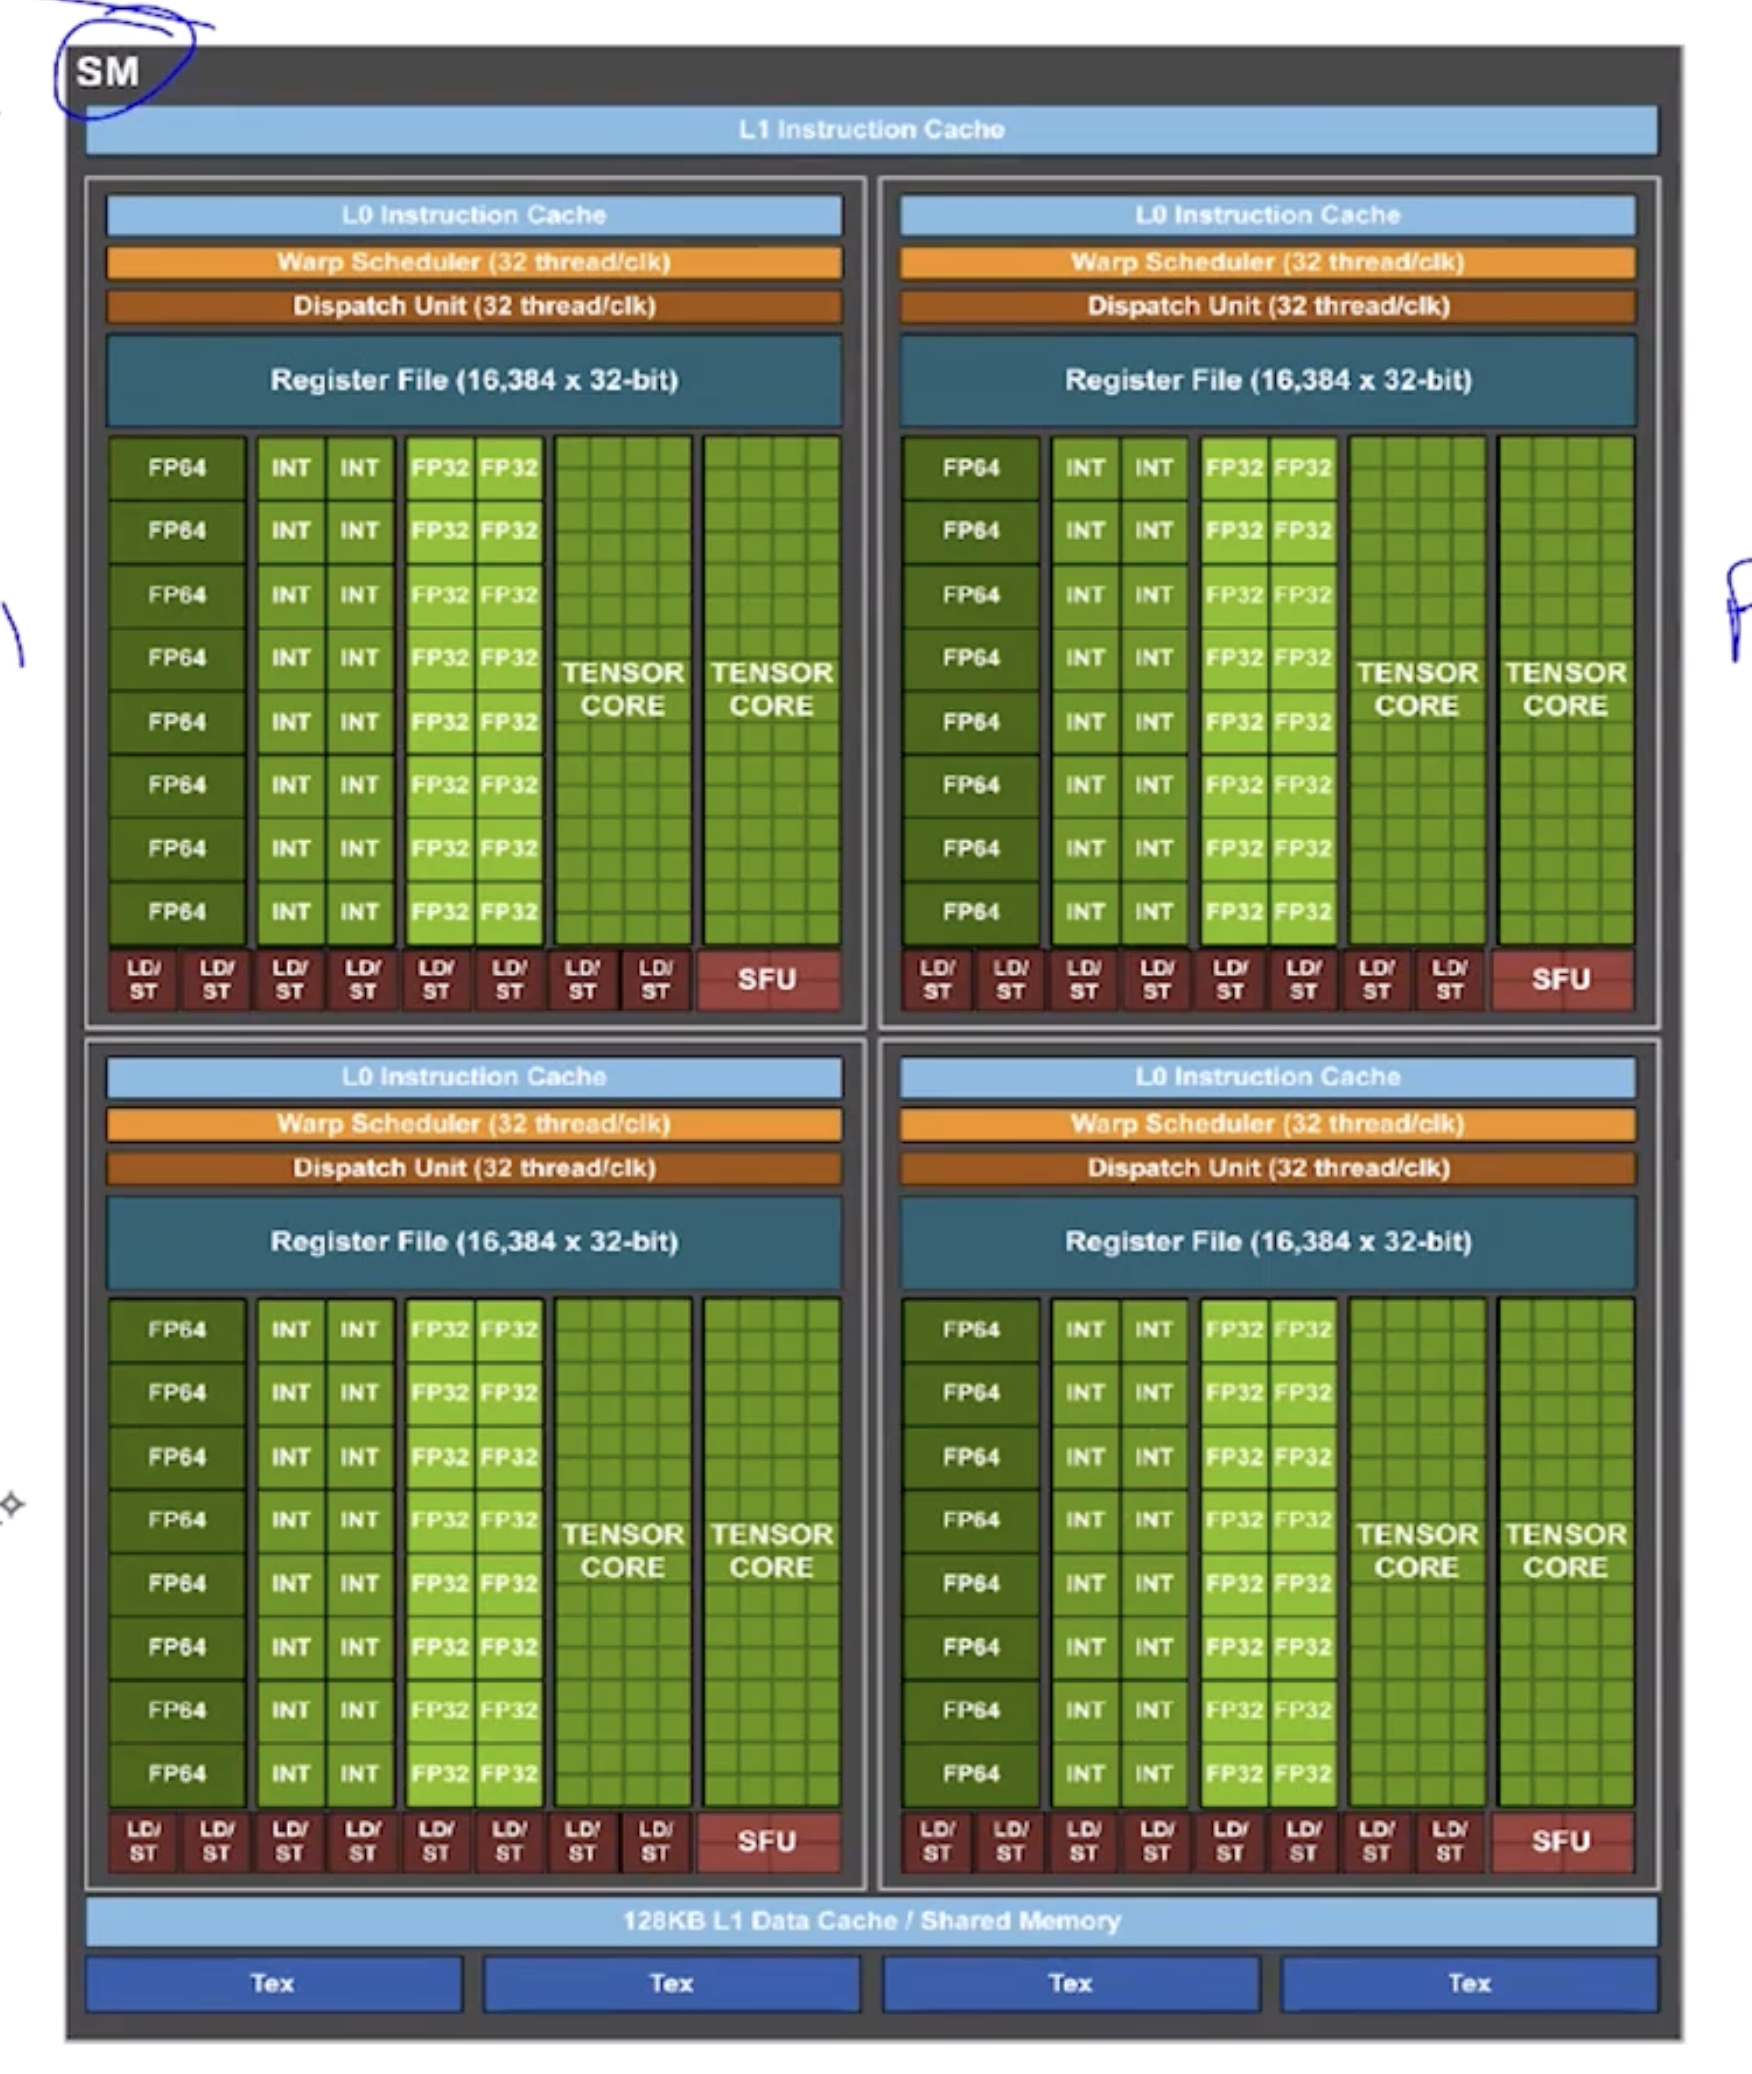
\includegraphics[width=0.75\linewidth]{resources/cuda-053.png}
    \caption{SM 内部架构}
    \label{fig:placeholder}
\end{figure}


\begin{itemize}
    \item \textbf{L0 指令高速缓存}：存储待执行指令。
    \item \textbf{Warp 调度器}：负责管理线程束（Warp，即 32 个线程为一组）。采用 SIMT（单指令多线程）模式，即一个 Warp 内的 32 个线程在不同核心上并行执行相同指令。
    \item \textbf{分发器（Dispatch Unit）}：与调度器协同，将指令分发到执行单元。
    \item \textbf{寄存器文件}：保存临时数据。
    \item \textbf{执行单元}：包括单精度/整数核心、张量核心及特殊功能单元（SFU）。
\end{itemize}

四个分区共享同一个 L1 高速缓存、共享内存和纹理内存。

\subsection{架构对比与NVLink}

让我们参考 A100 白皮书中的对比表来比较 Ampere、Volta 和 Pascal 架构：

\begin{figure}
    \centering
    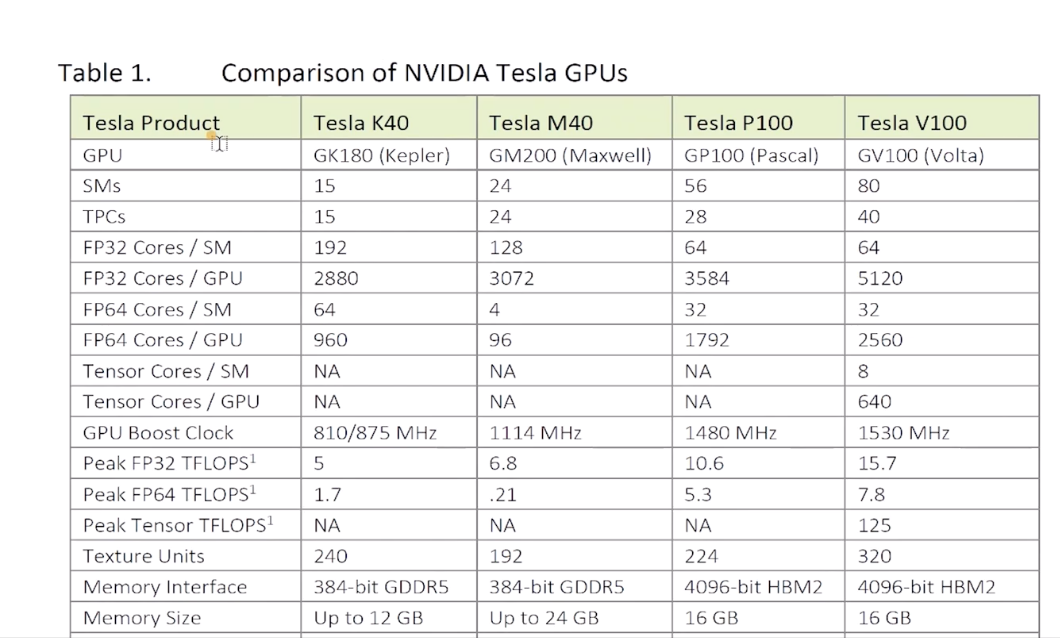
\includegraphics[width=0.75\linewidth]{resources/cuda-054.png}
    \caption{架构对比}
    \label{fig:placeholder}
\end{figure}


\begin{itemize}
    \item \textbf{SM 数量}：Pascal (56) $\rightarrow$ Volta (80) $\rightarrow$ Ampere (108)。
    \item \textbf{单精度核心}：Pascal ($\sim$3500) $\rightarrow$ Volta ($\sim$5000) $\rightarrow$ Ampere ($\sim$7000)。
    \item \textbf{整数核心}：Pascal 无独立整数核心（与浮点共用）；Volta ($\sim$5000)；Ampere ($\sim$7000)。
    \item \textbf{张量核心}：Pascal 无；Volta (640)；Ampere (432)。注意：虽然 Ampere 张量核心数量少于 Volta，但其单核能力和效率大幅提升，整体吞吐量反而是 Volta 的两倍以上。评估性能不能只看核心数量，还要看核心能力。
    \item \textbf{FP16 吞吐量（带 FP32 累加）}：Ampere 远超 Volta。这里涉及“使用单精度累加的半精度计算”概念，即输入为 FP16，但输出/累加使用 FP32 以保证精度。
    \item \textbf{常规单精度吞吐量}：Pascal (21\,TFLOPS) $\rightarrow$ Volta (31\,TFLOPS) $\rightarrow$ Ampere (78\,TFLOPS)。
    \item \textbf{显存位宽}：Volta ($\sim$4096-bit) vs Ampere ($>$5120-bit)。
    \item \textbf{显存容量}：Volta (16/32\,GB) vs Ampere (40\,GB)。
    \item \textbf{内存带宽}：Pascal ($\sim$700\,GB/s) $\rightarrow$ Volta (900\,GB/s) $\rightarrow$ Ampere (1500\,GB/s)。带宽受显存大小、速度和位宽共同影响。
    \item \textbf{L2 缓存}：Volta (6\,MB) $\rightarrow$ Ampere (40\,MB)，增长超 7 倍。
    \item \textbf{晶体管数}：Volta (210 亿) $\rightarrow$ Ampere (540 亿)。工艺从 Volta 的 12\,nm 演进到 Ampere 的 7\,nm。
\end{itemize}

\begin{figure}
    \centering
    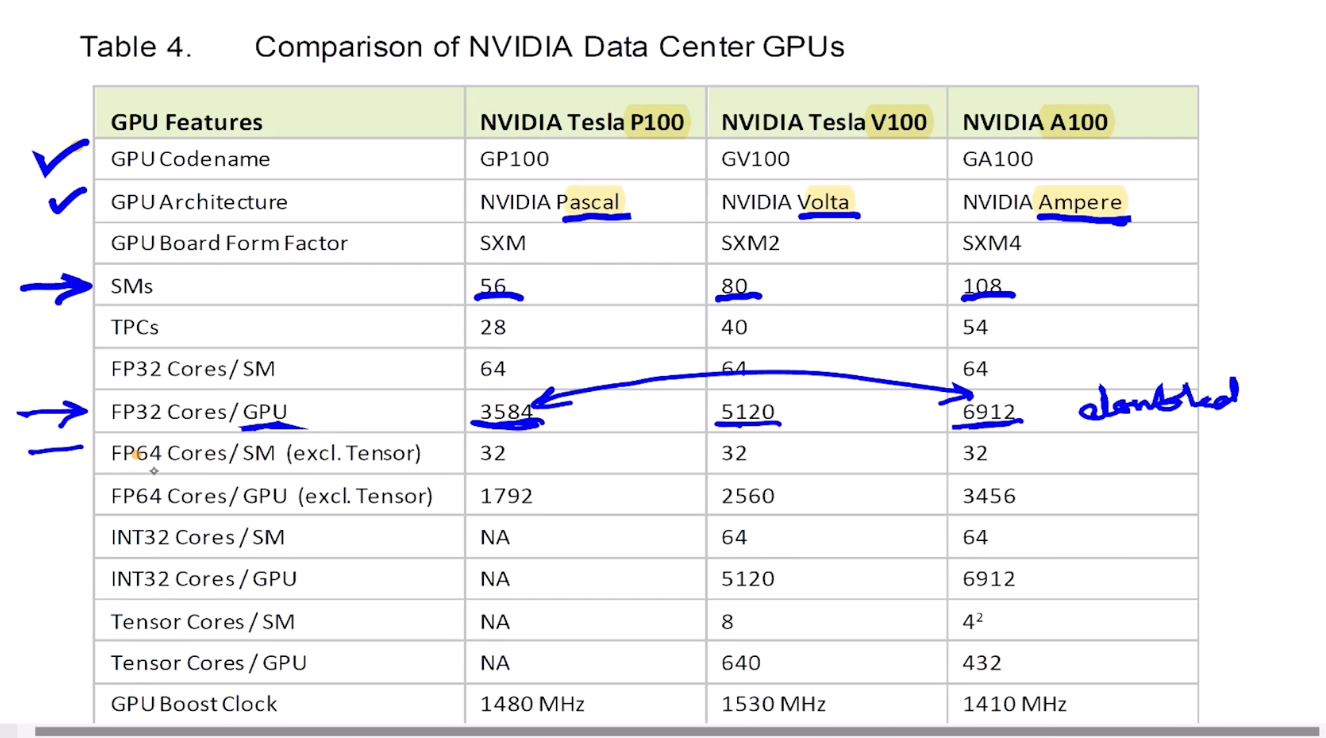
\includegraphics[width=0.75\linewidth]{resources/cuda-055.png}
    \caption{架构对比}
    \label{fig:placeholder}
\end{figure}


编写 CUDA 程序时，还需参考"CUDA 计算能力"表，了解最大线程数、最大块数等硬件限制。如果应用规模超出限制，需将其拆
分为多个核函数（kernel）执行。

\begin{figure}
    \centering
    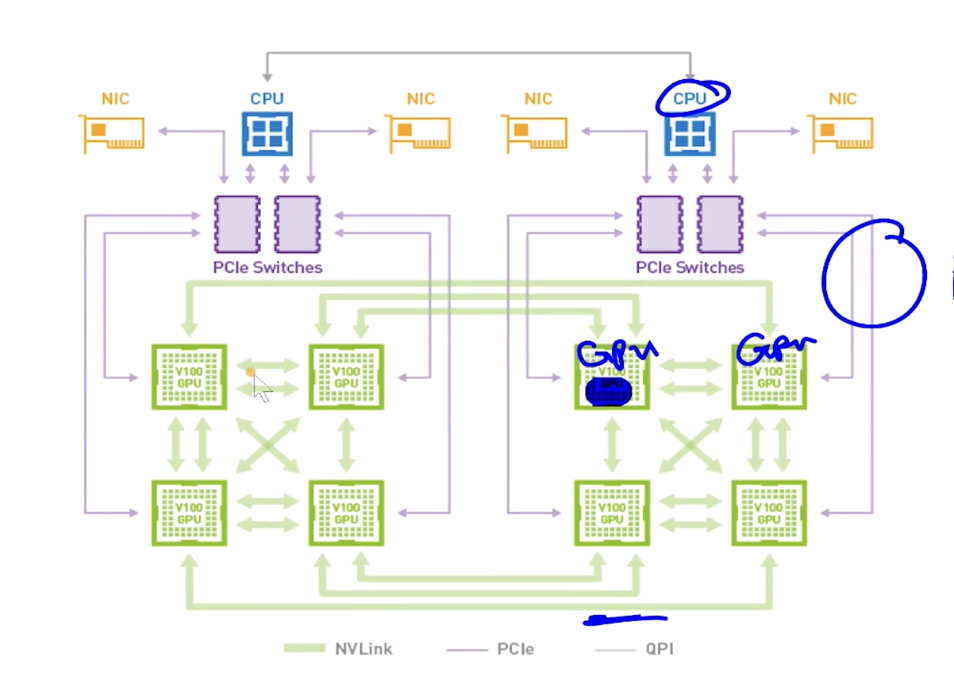
\includegraphics[width=0.75\linewidth]{resources/cuda-056.png}
    \caption{NVLink}
    \label{fig:placeholder}
\end{figure}


关于 \textbf{NVLink}：这是一种高速互联技术。第二代 NVLink 相比 Pascal的第一代有两大改进：
一是链路数量增加（GPU 间从 1 条增至 2 条以上）；二是链路速度提升。这使得 GPU间通信带宽从 Pascal 的 160\,GB/s 提升
至 Volta 的 300\,GB/s。NVLink 是 DGX服务器的标准特性。例如 DGX Station（4 块 V100）和 DGX-1（8 块 V100）。
对比 DGX-1的 Pascal 和 Volta 版本，虽然整机功耗同为 3200\,W，但 Volta版本凭借张量核心在同等能耗下提供了数倍于 Pascal 的计算性能
（能效比提升）。

本章涵盖了 Volta 架构的重点，并对比了 Pascal 和 Ampere。建议读者继续阅读白皮书剩余部分。


\section{CUDA 工具包概述}

欢迎大家。今天我们将深入探讨 CUDA 工具包。CUDA 工具包是 GPU编程领域的基石，正在革命性地改变高性能计算和深
度学习应用。CUDA（Compute Unified Device Architecture，统一计算设备架构）是英伟达的
并行计算平台。这个工具包不仅仅是一套工具的集合，更是开启英伟达GPU 巨大潜力的大门。让我们探索其关键组件，并了解它们如
何使我们能够充分利用 GPU 计算的全部能力。

\begin{figure}
    \centering
    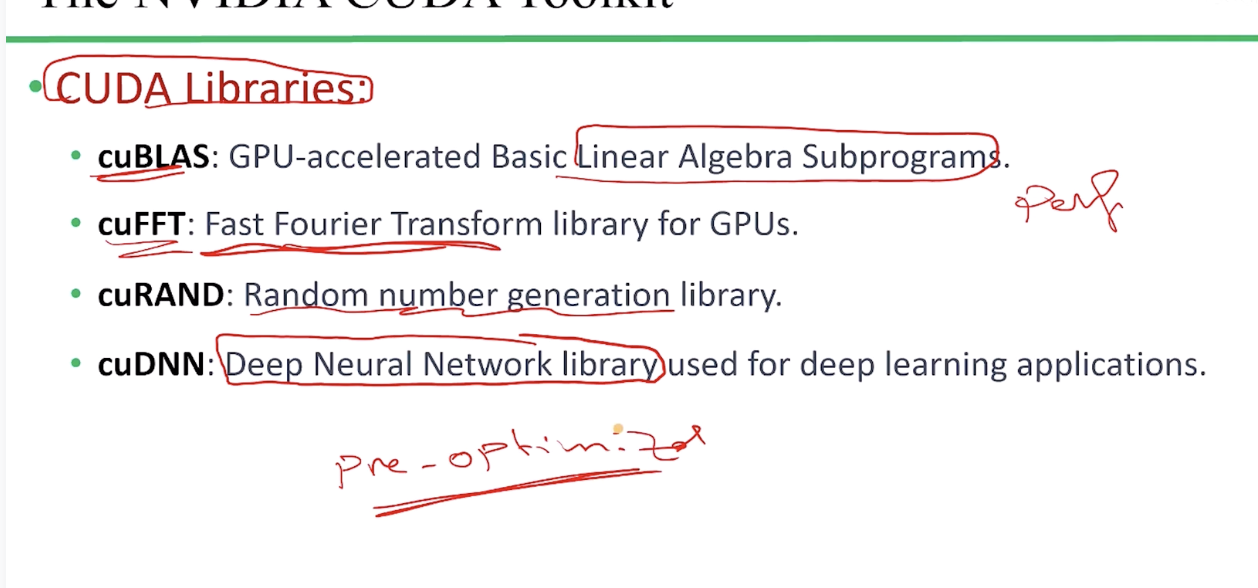
\includegraphics[width=0.75\linewidth]{resources/cuda-057.png}
    \caption{}
    \label{fig:placeholder}
\end{figure}

\subsection{nvcc编译器}

CUDA 开发的核心是 CUDA 编译器，即 \texttt{nvcc}编译器。它供开发人员、研究人员以及专业人士使用，
以简化从简单的 CUDA 编码到复杂 GPU应用程序的一切工作。该编译器是将高级 CUDA 代码转换为 GPU 可理解形
式的关键：它可以将 CUDA代码转换为与各种英伟达架构兼容的 PTX 代码。简而言之，\texttt{nvcc} 编译器
用于将 CUDA代码转换为可以在 GPU 上高效运行的可执行文件。

\subsection{优化库}

CUDA 拥有一套优化库的支持，每个库都有其专门用途。例如，\textbf{cuBLAS} 和\textbf{cuFFT}分别在线性代数
和快速傅里叶变换运算方面表现突出。这些库经过高度优化，能显著提升性能。此外还有\textbf{curand} 库，专门用于随机数生成；
以及 \textbf{cuDNN}库，这是一个为神经网络加速设计的深度学习库。这些库是高效 GPU编程的支柱，提供了预先优化的即用型函数，节省开发时间并增强性能。


\begin{figure}
    \centering
    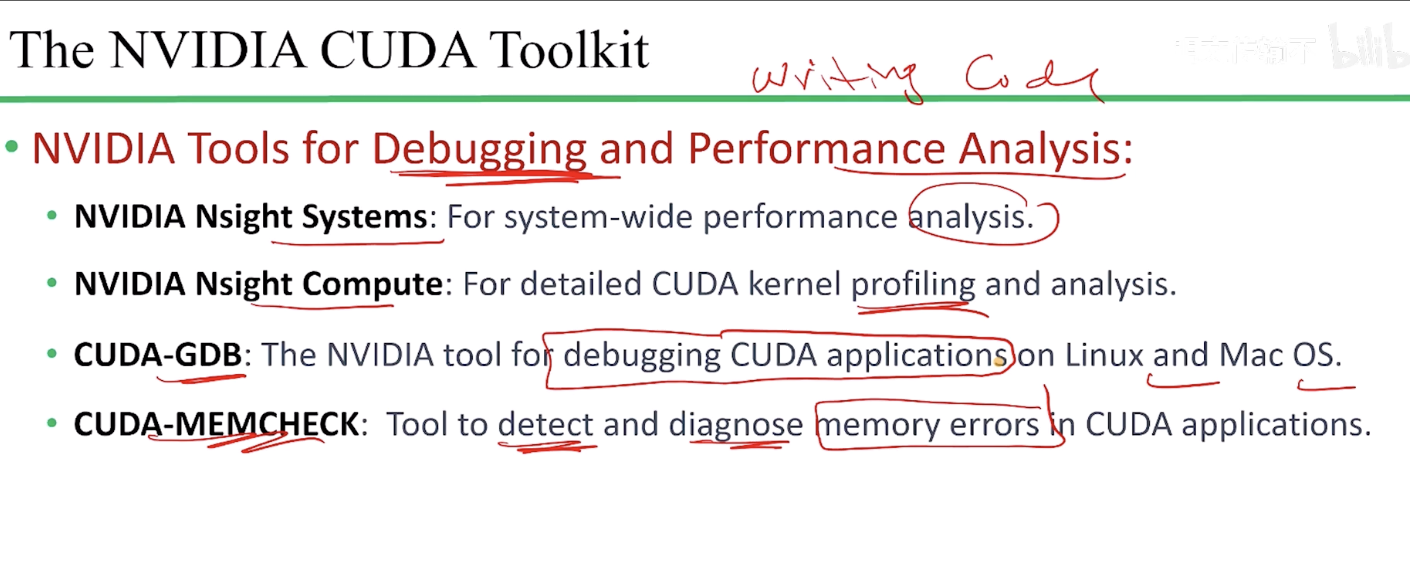
\includegraphics[width=0.75\linewidth]{resources/cuda-058.png}
    \caption{}
    \label{fig:placeholder}
\end{figure}

\subsection{运行时API}

CUDA 工具包还提供了运行时 API（RuntimeAPI），用于管理设备初始化、内存分配以及内核启动。它们对于管理应
用程序与 GPU 的交互至关重要。例如，对于 CPU和 GPU 之间的内存操作或数据传输，我们可以使用以下 API 函数：

\begin{itemize}
    \item \texttt{cudaMalloc}：在 GPU 设备上分配指定大小的内存。这类似于标准 C 语言中的 \texttt{malloc}，但专用于 GPU 而非 CPU 内存分配。
    \item \texttt{cudaMemcpy}：用于在主机（CPU）和设备（GPU）之间复制数据。
\end{itemize}

以上是运行时 API 函数的两个典型示例。
\subsection{调试与分析工具}

在这张幻灯片中我想强调，对于 GPU应用程序来说，工作不止于编写代码，还关乎确保效率和稳定性。这就是为什么英伟达工具包含了强大的工具：
\begin{itemize}
    \item \textbf{Nsight Systems} 和 \textbf{Nsight Compute}：用于分析和剖析应用程序的性能。
    \item \textbf{cuda-gdb}：提供在 Linux 和 macOS 操作系统上调试 CUDA 应用程序的强大环境。
    \item \textbf{cuda-memcheck}：专门用于检测和诊断内存问题的工具。
\end{itemize}
所有这些工具共同提供了一个全面的环境，不仅用于编写代码，还用于完善和优化 GPU 加速应用程序。

\begin{figure}
    \centering
    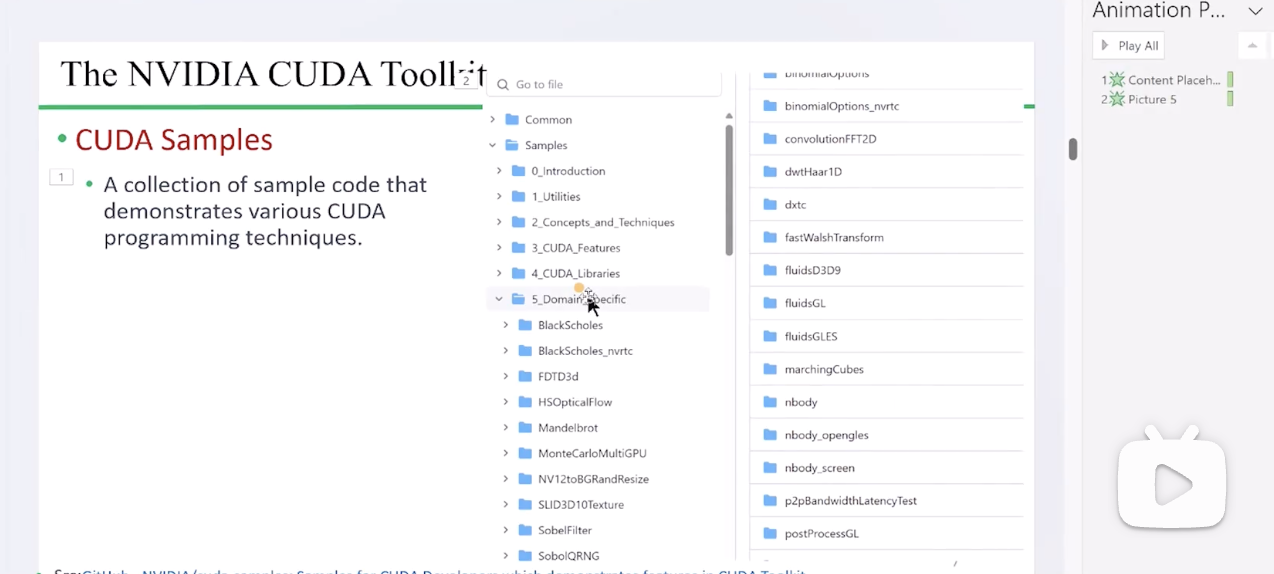
\includegraphics[width=0.75\linewidth]{resources/cuda-059.png}
    \caption{}
    \label{fig:placeholder}
\end{figure}


\subsection{示例代码}

CUDA 工具包附带了一套丰富的示例代码。这些示例不仅仅是代码，更是实用的指南，阐明了各种 CUDA编程技术，从基本概念
到高级操作，涵盖了广泛的场景和应用案例。这些示例可以提供对高效 CUDA编程的宝贵见解，提供一种实用的学习体验，补充理论
知识。

在本文章的最后，我想总结：CUDA 工具包不仅仅是编译 GPU 应用程序的编译器，或是编写 CUDA程序的编辑器。它是一
个综合平台，包含了编写、编辑、编译和剖析 GPU 应用程序所需的一切。


\section{在 Linux 系统上安装 CUDA 工具包}

本章讲解如何在 Linux 系统上安装 CUDA 工具包。假设你正在使用前文介绍过的 WSL 工具，首先打开"开始"菜单，搜索"命令
提示符"并点击打开，然后输入 \texttt{wsl} 即可在当前 Windows 系统上启动 Linux 子系统。

\subsection{检查nvcc}

现在检查 \texttt{nvcc} 编译器是否已安装在 Ubuntu 系统中。启动 Ubuntu 后，终端提示 \texttt{command not found}，
说明 \texttt{nvcc} 尚未安装。

\begin{figure}
    \centering
    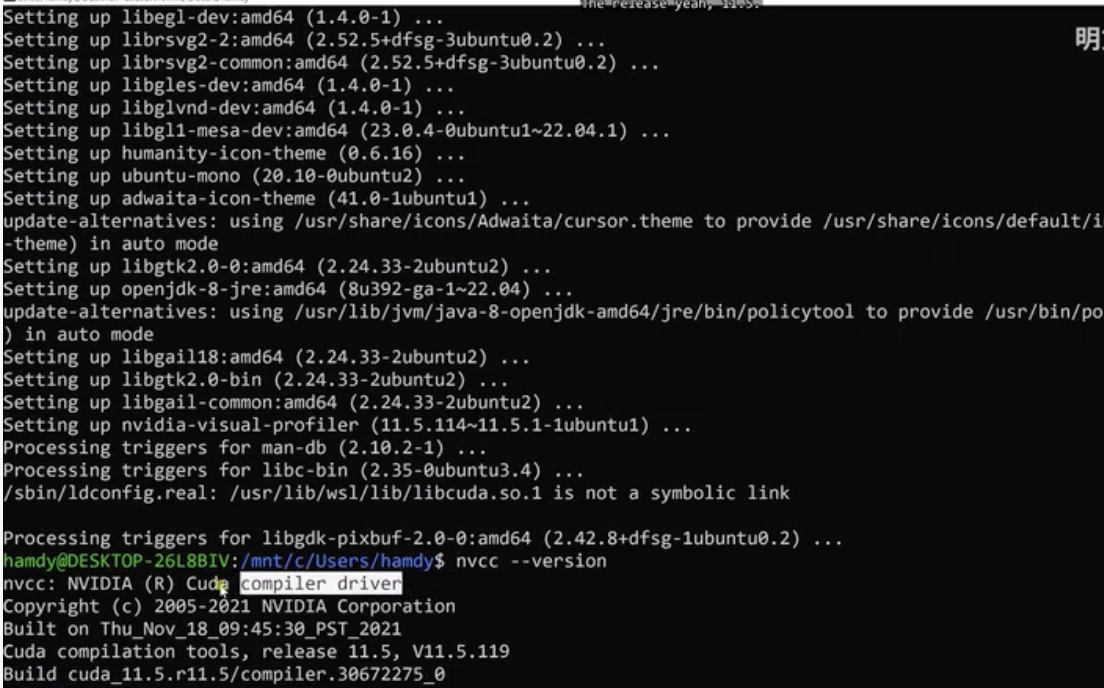
\includegraphics[width=0.75\linewidth]{resources/cuda-060.png}
    \caption{}
    \label{fig:placeholder}
\end{figure}

\subsection{安装CUDA工具包}

需要安装 CUDA 工具包才能使用 \texttt{nvcc} 编译器。打开 CUDA 工具包下载页面，选择操作系统、架构以及发行版本。
有多种发行版可选，这里选择 Ubuntu；如果你使用的是 WSL，也可以选择 WSL-Ubuntu。接着会看到三个安装选项：其中两个
先下载本地安装包（标为 Local），中间那个则是通过网络直接安装（Network）。不过，最简单、最不容易出错的方式是直接使
用 \texttt{apt} 安装。

再检查一次 \texttt{nvcc} 版本，虽然提示命令未找到，但第二行给出了安装建议：
\begin{verbatim}
sudo apt install nvidia-cuda-toolkit
\end{verbatim}

复制这条指令并在终端中输入，然后输入密码。系统会询问是否继续，输入 Y 确认即可。安装过程大约需要 30-40 分钟，请耐心等
待。CUDA 工具包安装完成后，你将拥有 \texttt{nvcc} 编译器以及前文介绍的所有其他功能。再次检查 \texttt{nvcc} 编译器版
本，可以看到 CUDA 编译器已成功安装（版本 11.5），输出第一行显示 \texttt{nvcc: NVIDIA (R) Cuda compiler driver}，
表示 CUDA 工具包已就绪，对入门来说已经足够了。

另外提醒一点：如果你按照官网的步骤操作，可能会遇到一些依赖问题或错误。因此建议一开始先使用上述 \texttt{apt} 指令，它简
单且不易出错。等你熟悉之后，需要更新 CUDA 工具包时，再到 CUDA 官网选择适合你系统的最新版本进行安装。


\section{NVIDIA GPU 硬件与软件层级结构及 CUDA 介绍}

本章将深入探讨 NVIDIA GPU 的硬件与软件层级结构，并介绍 CUDA。

CUDA 全称为 Compute Unified Device Architecture（统一计算设备架构），是由 NVIDIA 开发的一个并行计算平台和应用程序编程
接口（API）。CUDA 允许软件开发者使用 NVIDIA 的图形处理单元进行通用目的计算，这种方法被称为 GPGPU（General-Purpose 
computing on Graphics Processing Units，即图形处理单元上的通用计算）。

在开始之前，强调三个关键点。第一，CUDA 基于 C 编程语言，这是一个优势，它让熟悉 C 语言的开发者能够轻松编写可在 
NVIDIA GPU 上执行的软件。第二是 CUDA 编译器 \texttt{nvcc}——它不仅仅是一个普通的编译器，而是 CUDA 工具包的核心。
\texttt{nvcc} 的作用远不止将 CUDA 代码转换为可执行文件或机器码，它在开发过程中扮演着多重关键角色。随着本课程的推进，
我们将逐步揭示 \texttt{nvcc} 的多功能性，以及它如何优化 CUDA 应用程序。

第三点是主机（Host）与设备（Device）这两个术语的区别，这是为了充分利用 GPU 的资源。通常，主机指的是 CPU 及其关联的
全局内存（即 RAM），而设备则指 GPU 及其全局内存。这种区分不仅在术语上非常重要，在编写软件的方式上也至关重要——它影响
代码结构、数据传输和内存管理。本图中左侧部分代表主机，右侧部分代表设备（即 GPU）。

\begin{figure}
    \centering
    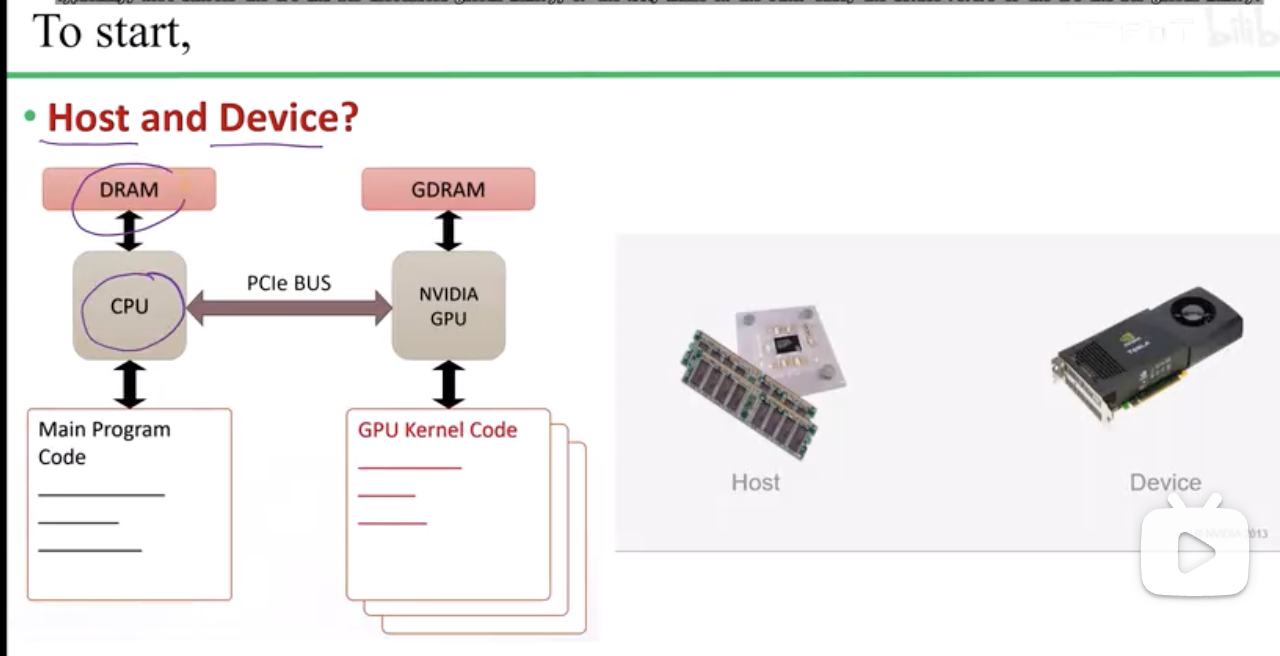
\includegraphics[width=0.75\linewidth]{resources/cuda-061.png}
    \caption{}
    \label{fig:placeholder}
\end{figure}

\subsection{硬件四级层级}

回顾 GPU 硬件架构层级与其软件部分之间的关系。GPU 的结构包含四个明确的硬件组织层级，且是分层的：最顶层是 GPU 本身
，它封装了所有单元；每个 SM（Streaming Multiprocessor，流式多处理器）构成该层级结构的第二级。这一设计已在 Volta 
白皮书章节中详细说明。

接着，每个 SM 又被进一步划分为若干个分区（Sub-partition / Processing Block），构成硬件结构的第三级。在 Volta 和 
Ampere 架构中，每个 SM 包含四个这样的分区。如图所示，来自 Volta 白皮书的图中 SM 被划分为四个分区。Ampere 白皮书
中也能看到类似的结构。

\begin{figure}
    \centering
    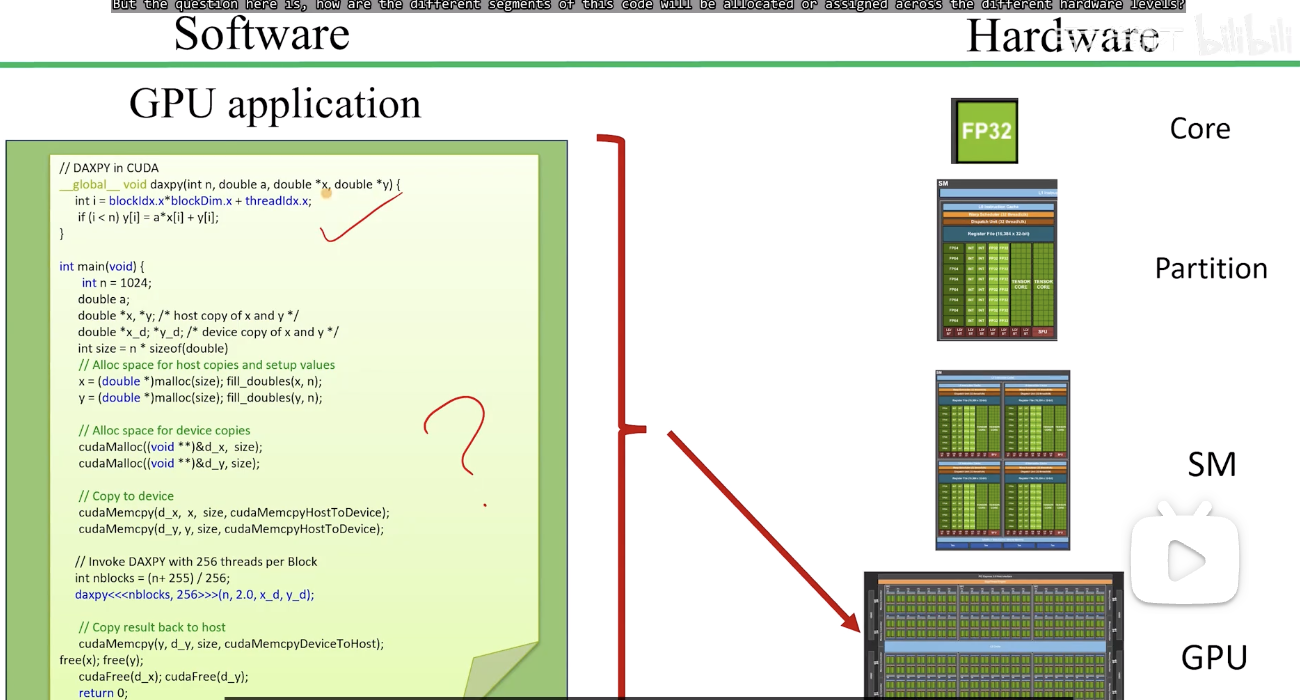
\includegraphics[width=0.75\linewidth]{resources/cuda-062.png}
    \caption{}
    \label{fig:placeholder}
\end{figure}


在第四级（最细粒度的层级），每个分区内包含独立的计算单元，例如负责执行浮点运算的 FP32 核心。这些核心是 GPU 内部处理
计算的基本单元。

综上所述，GPU 的硬件架构可视为一个四级层级结构：从整个 GPU 开始逐级向下，经过 SM，再到其内部的分区作为第三级，最终到
达各个独立的计算核心。这些不同的硬件层级反过来要求对应的软件应用程序具备相似的结构。

例如，假设我们有一个 CUDA 应用程序（如图所示，用方框表示），该应用程序设计用于在整个 GPU 上运行。问题是：这段代码的
不同部分将如何分配或指派到不同的硬件层级？这正是需要理解的内容——软件代码的不同部分如何映射到硬件的不同层级。

\begin{figure}
    \centering
    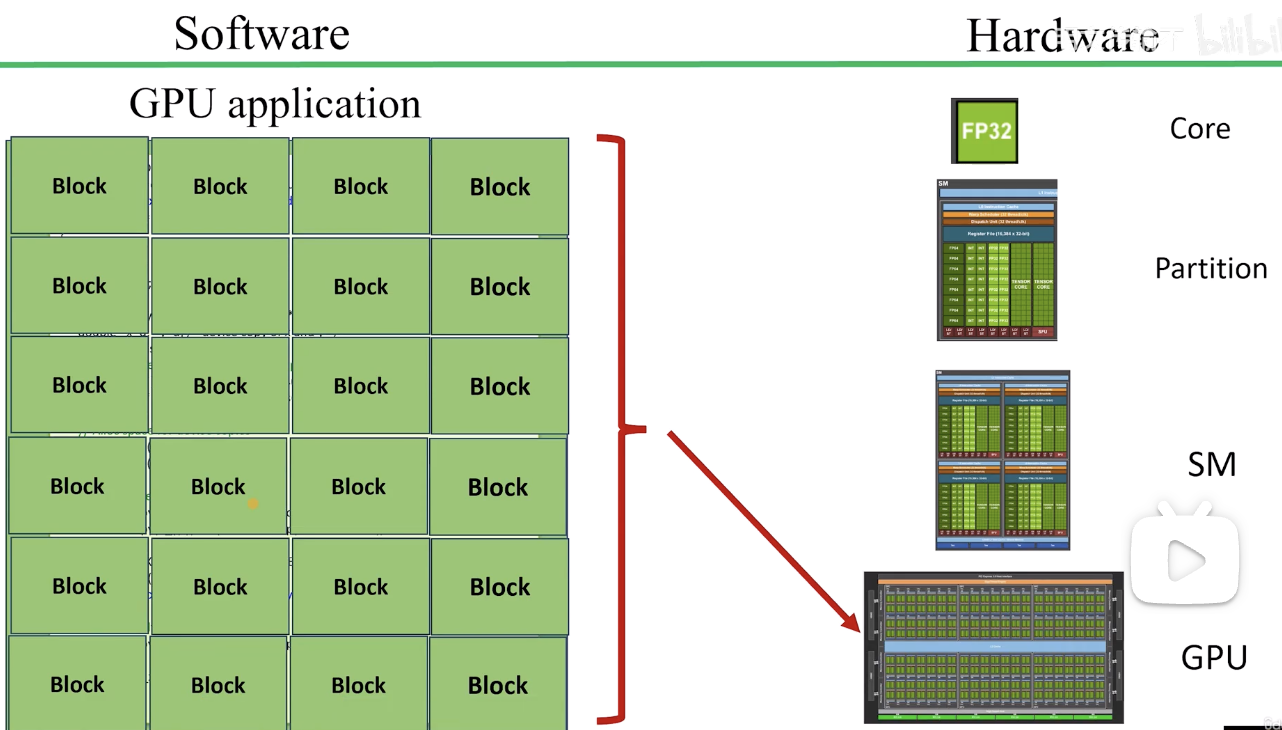
\includegraphics[width=0.75\linewidth]{resources/cuda-063.png}
    \caption{}
    \label{fig:placeholder}
\end{figure}


\subsection{软件层级：块与GigaThread Engine}

编写 CUDA 代码的第一步是将 GPU 核函数（Kernel）划分成更小的软件单元，称为块（Block）或线程块（Thread Block）。对于每
个核函数，首先需要配置其块数量。如果将整个方框视为一个 CUDA 应用程序，就可以将其划分为更小的块。如图所示，每个小方框
代表一个块（或线程块，两个名称均正确）。这种划分对应了 GPU 的前两个硬件层级——整个应用程序设计用于在整个 GPU 上执行。

然而这引发了一个问题：软件中的第二级是指不同的块在不同的 SM 上执行。在左侧，有由软件块（线程块）表示的任务；在另一侧
，有可视为"工人"的 SM。谁负责将这些软件任务分配给工人（SM）？

\begin{figure}
    \centering
    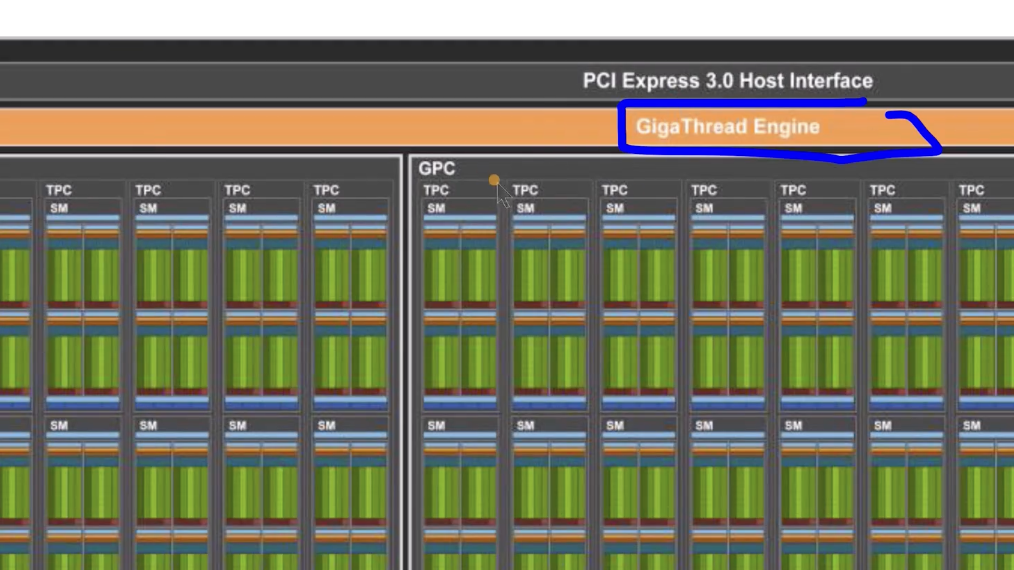
\includegraphics[width=0.75\linewidth]{resources/cuda-064.png}
    \caption{}
    \label{fig:placeholder}
\end{figure}


要回答这个问题，需要了解另一个单元——GigaThread Engine。它是 GPU 内部最重要的单元之一，其关键功能就是高效地将这些软
件块（任务/作业）分配到各个 SM 上。参考 Volta 白皮书可以看到，GigaThread Engine 位于整个 GPU 的整体结构之中，并连接到
所有 SM——它负责为这些 SM 提供必要的软件块或软件任务。

将同样的原理应用到下一层级。假设图中的第一个块被分配到某个 SM 上执行，但该 SM 中有四个分区，而我们这里只有一个块。这
个被称为"块"的单一软件单元应如何分配到 SM 内部的四个硬件分区中？

如果将整个块只分配给其中一个分区，就会导致资源利用率不足（三个分区空闲）。这一考虑引出了软件层级的第三级——Warp（线程束），以避免浪费可用的硬件资源。

\begin{figure}
    \centering
    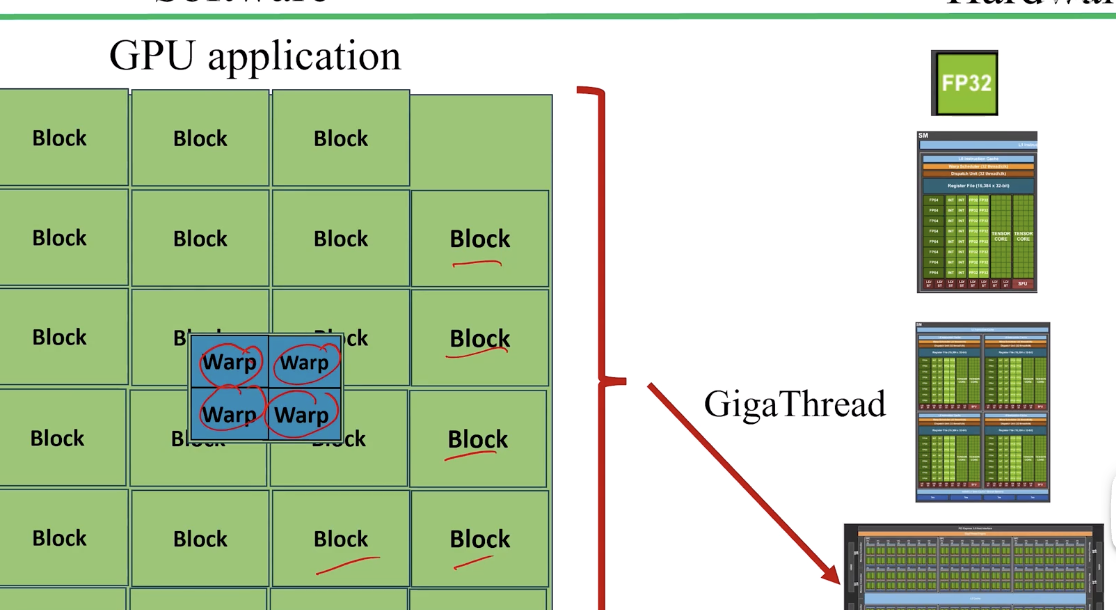
\includegraphics[width=0.75\linewidth]{resources/cuda-065.png}
    \caption{}
    \label{fig:placeholder}
\end{figure}

\subsection{Warp与调度}

每个软件块都会被细分为更小的单元，称为 Warp。例如，如果将第一个块划分为四个 Warp，那么每个 Warp 就可以分配到 SM 中的
一个不同分区——四个 Warp 对应四个分区，每个分区分配一个 Warp。

考虑另一个例子：如果每个块有 32 个 Warp，而有四个分区，那么每个分区将执行八个 Warp。当一个分区分配了多个 Warp 时，就
需要一个管理者——这就是为什么每个分区中都有一个 Warp Scheduler（Warp 调度器）单元。

放大该分区，可以看到内部的 Warp 调度器单元。正如前文所述，该单元存在于每个分区中，负责在每个时钟周期中调度某个 Warp
。这是在硬件层面；而在软件层面，一个 Warp 默认通常由 32 个线程组成。

进入第四级，每个分区包含若干个核心。Warp 中的每个线程会在分区内独立的核心上执行，确保每个核心都积极参与计算。理解硬件
和软件中的这四个层级，对于高效配置 CUDA 应用程序至关重要。

块的数量以及每个块中的线程数量，是启动任何 CUDA 应用程序时需要指定的两个关键参数（将在后续章节中详细探讨）。关于 Warp
，可以通过将块大小（即每个块的线程数）除以 32 来计算每个块中的 Warp 数量，因为 Warp 的大小固定为 32 个线程。


\section{第一个 CUDA 项目：核函数与执行配置}

本章将开始第一个项目——打印块和线程的 ID。这是一个非常简单的项目。从开始菜单启动 Visual Studio，创建一个新项目。在项目中
选择 CUDA 语言，然后为你的项目命名（例如 \texttt{test\_01}），点击创建。

\subsection{项目创建与核函数}

这是第一个项目，核函数文件默认为 \texttt{kernel.cu}。删除模板中的所有代码，只保留已准备好的几行头文件包含代码。本节不关注头文件部分，只关注核心代码。

假设读者已具备 C 编程语言的基础。本应用程序中有两个核函数，或者说一个核函数和一个普通函数。普通函数是主函数（\texttt{main}）——每个 C 程序都必须包含主函数，而 CUDA 代码基于 C，因此同样需要主函数。

核函数（Kernel）是将在 GPU 上执行的函数，而普通函数则在 CPU 上执行。区分两者的标志是 \texttt{\_\_global\_\_} 修饰符——带有该修饰符的即为核函数。其声明方式与普通函数类似：有返回类型、函数名、括号和大括号。当前这是一个空核函数，接下来将填充具体内容。

主函数中包含两条指令：第一条是核函数调用，第二条是 \texttt{return 0}——因为主函数类型为 \texttt{int}，所以必须返回一个整数值。

\subsection{执行配置参数}

调用核函数时，需要写出核函数名称，并配置执行参数（将影响应用程序的输出）。核函数还可以接收输入参数，例如后续章节中将对两个向量进行相加，需要在核函数中传入这些向量。本节不涉及输入参数。

本程序包含一个核函数和一个主函数，主函数调用核函数以在 GPU 上执行。

目标是打印块和线程的 ID。使用 \texttt{printf} 函数即可实现：以 \texttt{\textbackslash n} 开头换行，然后以 \texttt{\%d} 格式输出线程 ID 和块 ID，最后传入对应的变量。

CUDA 提供了预定义的块和线程索引变量：\texttt{blockIdx} 提供块 ID，\texttt{threadIdx} 提供线程 ID。CUDA 支持多维索引，本节只使用一维（\texttt{.x}）。例如，如果程序中有十个块，\texttt{blockIdx.x} 将打印从 0 到 9 的 ID。

核函数编写完成后，点击"生成（Build）"→"生成解决方案（Build Solution）"即可编译。Windows 下 Visual Studio 会自动调用 \texttt{nvcc} 编译器；Linux 用户则需要学习使用 \texttt{nvcc} 命令行编译（将在后续章节中讲解）。

核函数调用语法如下：

\texttt{核函数名<<<块数量, 每块线程数>>>();}

其中，尖括号 \texttt{<<<>>>} 内的第一个参数是网格中的块总数，第二个参数是每个块中的线程数（注意：这不是应用程序的线程总数）。当前配置为 \texttt{<<<1,1>>>}，即只有一个块、一个线程，因此输出块 ID 为 0、线程 ID 为 0。

将每块线程数增加为 4，重新构建并运行：

\begin{figure}
    \centering
    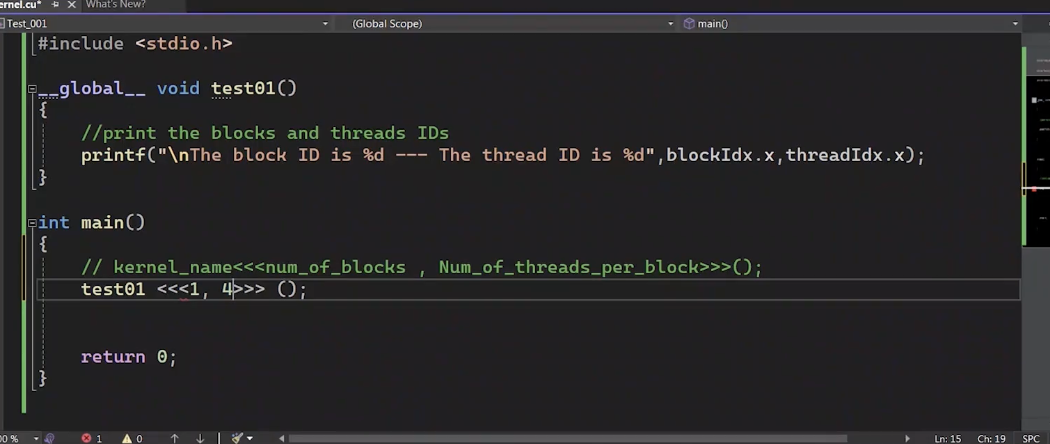
\includegraphics[width=0.75\linewidth]{resources/cuda-066.png}
    \caption{}
    \label{fig:placeholder}
\end{figure}

\subsection{逐步增加线程数与块数}

此时只有一个块，块 ID 为 0，四个线程 ID 从 0 到 3。将每块线程数增加到 32，重新构建并运行：


\begin{figure}
    \centering
    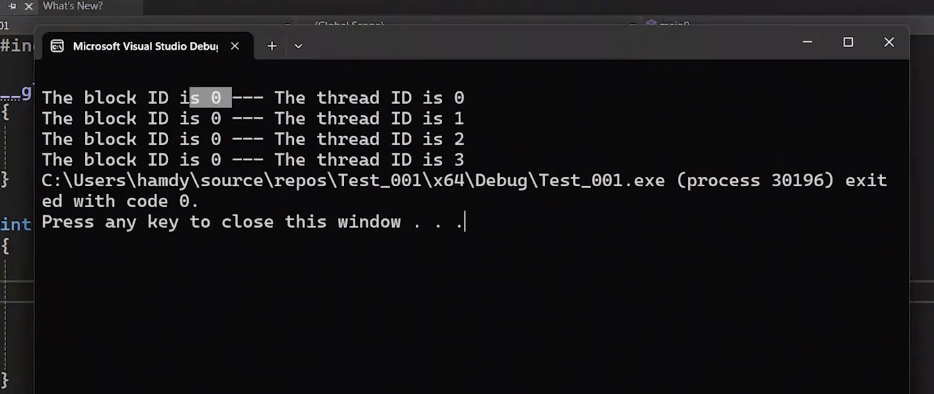
\includegraphics[width=0.75\linewidth]{resources/cuda-067.png}
    \caption{}
    \label{fig:placeholder}
\end{figure}

将块数量改为 2，每块线程数设为 8：

\begin{figure}
    \centering
    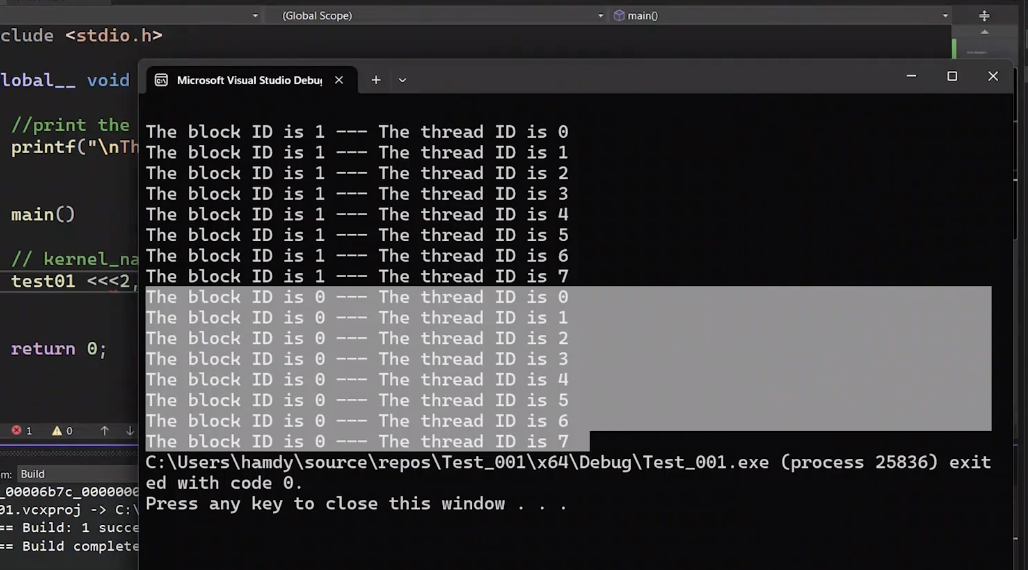
\includegraphics[width=0.75\linewidth]{resources/cuda-068.png}
    \caption{}
    \label{fig:placeholder}
\end{figure}

输出显示两个块（ID 分别为 0 和 1），每个块有 8 个线程（从 0 到 7）。你可能好奇为什么块 ID 1 先于块 ID 0 执行——这取决于哪个 SM 先接收到它的块，顺序并不重要。

接下来结合白皮书内容尝试更多配置。线程数量通常使用 2 的幂次，例如 512。将每块线程数设为 512 并运行：输出正常，块 ID 为 0，线程 ID 从 0 到 511。注意输出顺序可能不是连续的——因为线程是并行执行的，哪个线程先完成就哪个先输出，这是正常现象。

将每块线程数翻倍到 1024，运行正常，线程 ID 从 0 到 1023。再次翻倍设为 2048，运行：

\begin{figure}
    \centering
    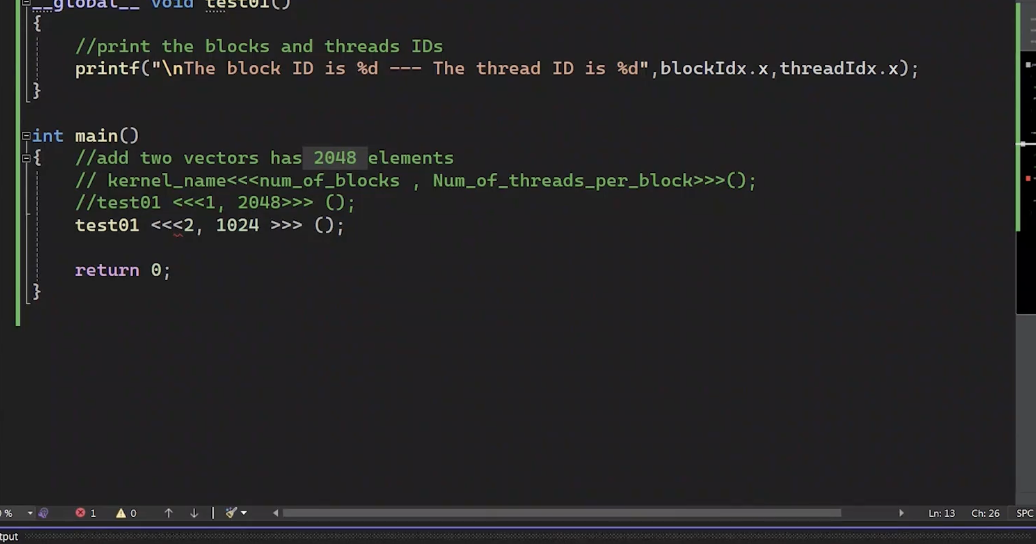
\includegraphics[width=0.75\linewidth]{resources/cuda-070.png}
    \caption{}
    \label{fig:placeholder}
\end{figure}


\subsection{硬件限制}

程序无法运行，没有任何输出。编译成功但运行失败，原因在于硬件限制。

以 Ampere 架构白皮书为例，其中的表格列出了最大线程数、最大 Warp 数、最大块数、最大寄存器数等限制。每个块的最大线程数（最大线程块大小）在 Ampere 架构中为 1024，这一限制适用于大多数架构。因此，不能将每块线程数设定为超过 1024。

这就是为什么需要同时理解软件和硬件。回到程序，假设需要对两个向量进行相加，每个向量包含 2048 个元素。如果将每块线程数设为 2048，程序将无法运行。解决方案是增加块的数量：将每块线程数设为 1024，块数设为 2（即 \texttt{<<<2, 1024>>>}），总线程数等于 $2 \times 1024 = 2048$，正好满足需求。运行后程序正常工作。

如果将块数设为 200 万，是否能运行？需要查阅白皮书中的限制。每个 SM 的最大线程块数为 32，但这是每个 SM 的限制，而非整个 GPU 的限制。整个 GPU 可运行的最大块数 = 每个 SM 最大块数 × SM 数量。例如，基于 GA100 芯片的 GPU 有 108 个 SM，因此最大并发块数为 $32 \times 108 = 3456$。

这就是软件配置与硬件限制之间的关系：每个块中的线程数与块的数量必须与硬件资源相匹配。



\section{在 Linux 系统上编译和运行 CUDA 程序}

本章讲解如何在 Linux 系统上编译和运行 CUDA 程序。请先阅读前一章的内容，因为本章不再重复解释相同的项目。

打开包含本章所有项目的文件夹，使用任意编辑器打开第一个项目 \texttt{project\_01}。例如，使用 Visual Studio Code 打开后，
可以看到一个 GPU 核函数，用于打印块 ID、线程 ID 和 Warp ID。我们使用两个块，每个块包含 64 个线程来启动该核函数。

\subsection{使用 nvcc 编译}

Visual Studio Code 本身只是编辑器，不具备编译功能。需要打开命令提示符，输入 \texttt{wsl} 在 Windows 上启动 Linux 子
系统（安装方法详见前文章节），然后进入项目文件夹。

使用 \texttt{nvcc --version} 可以检查 nvcc 编译器是否已安装。编译命令如下：

\begin{verbatim}
nvcc -o project_01 project_01.cu
\end{verbatim}

其中 \texttt{-o} 用于指定可执行文件的名称（建议在所有编译命令中都使用它）。编译完成后，输入 \texttt{ls} 即可看到生成的
可执行文件。

\subsection{运行程序与输出问题}

运行程序时，输入 \texttt{./project\_01} 并按回车。但有时终端上没有任何输出——项目本应为每个线程打印一行内容。

\begin{figure}
    \centering
    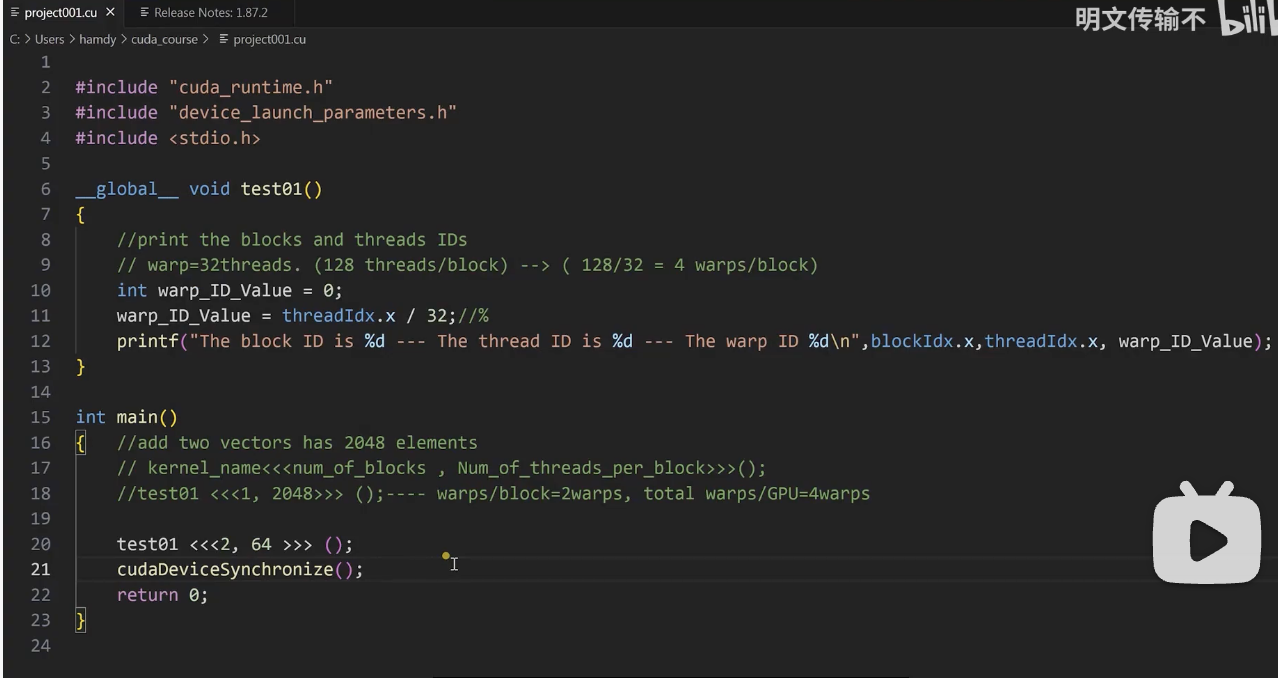
\includegraphics[width=0.75\linewidth]{resources/cuda-071.png}
    \caption{}
    \label{fig:placeholder}
\end{figure}

再运行一次，这次有输出了。程序本身没有问题，但第一次运行时终端上缺少输出，这是怎么回事？

\subsection{cudaDeviceSynchronize}

原因在于 CPU 与 GPU 的执行是异步的。在 CPU 一侧，主函数会逐条执行指令。当遇到启动 GPU 核函数的指令时，CPU 会将
核函数发送到 GPU，但不会等待 GPU 的执行结果，而是立即执行下一条指令。因此，GPU 的 \texttt{printf} 输出可能来不
及在程序结束前显示。

解决方案是使用 \texttt{cudaDeviceSynchronize()}——"同步"意味着让 CPU 等待，直到 GPU 完成核函数的执行。在核函数
调用之后添加这一行：

\begin{verbatim}
kernel<<<blocks, threads>>>();
cudaDeviceSynchronize();
\end{verbatim}

编译并运行后，每次都能看到完整的输出。不使用 \texttt{cudaDeviceSynchronize()} 时，输出时有时无；使用后则始终
稳定输出。

这一同步机制不仅适用于 Linux，也适用于 Windows。

\subsection{编译错误排查}

如果故意制造编译错误（例如删除某个分号），编译器会提示错误出现在某一行。需要注意的是：分号缺失通常会反映在下一条指令
上，因此应检查报错行的上一条语句。修正错误后保存并重新编译即可。

以上就是在 Linux 系统上编译和运行 CUDA 应用程序的完整流程。



\section{CUDA 课程项目二：线程束 ID（Warp ID）}

在前一个项目中，我们研究了块 ID（Block ID）和线程 ID（Thread ID）。本章将研究第三层级——\textbf{线程束 ID}（Warp ID）。

\subsection{Warp ID 概念}

每个 GPU 应用程序包含网格（Grid），网格包含块（Block），块包含线程束（Warp），每个线程束由 32 个线程组成。这就是 CUDA 程序中的四级软件层级结构。

\begin{figure}
    \centering
    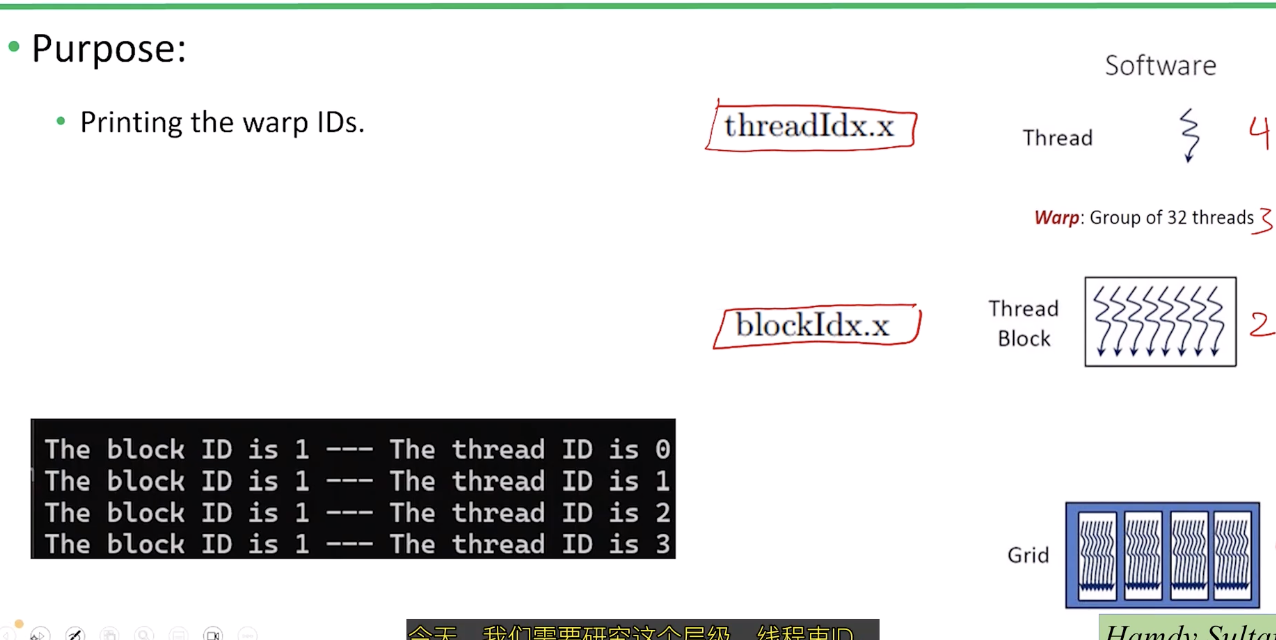
\includegraphics[width=0.75\linewidth]{resources/cuda-072.png}
    \caption{}
    \label{fig:placeholder}
\end{figure}

前文已经学习了如何打印线程 ID（X、Y、Z 三个维度）和块 ID。本章的目标是计算并打印线程束 ID。这里的关键问题是：CUDA 中\textbf{没有}预定义变量直接提供线程束 ID 值，需要我们自行计算。

\subsection{计算 Warp ID}

已知每个线程束由 32 个线程组成，如果每个块有 128 个线程，则每块有 $128 / 32 = 4$ 个线程束。

计算线程束 ID 的方法如下：声明变量 \texttt{WarpID}，将其初始化为 0，然后令其等于当前线程的线程 ID 除以 32。每个线程的线程 ID 不同，除法运算后得到该线程所属的线程束 ID。

\begin{figure}
    \centering
    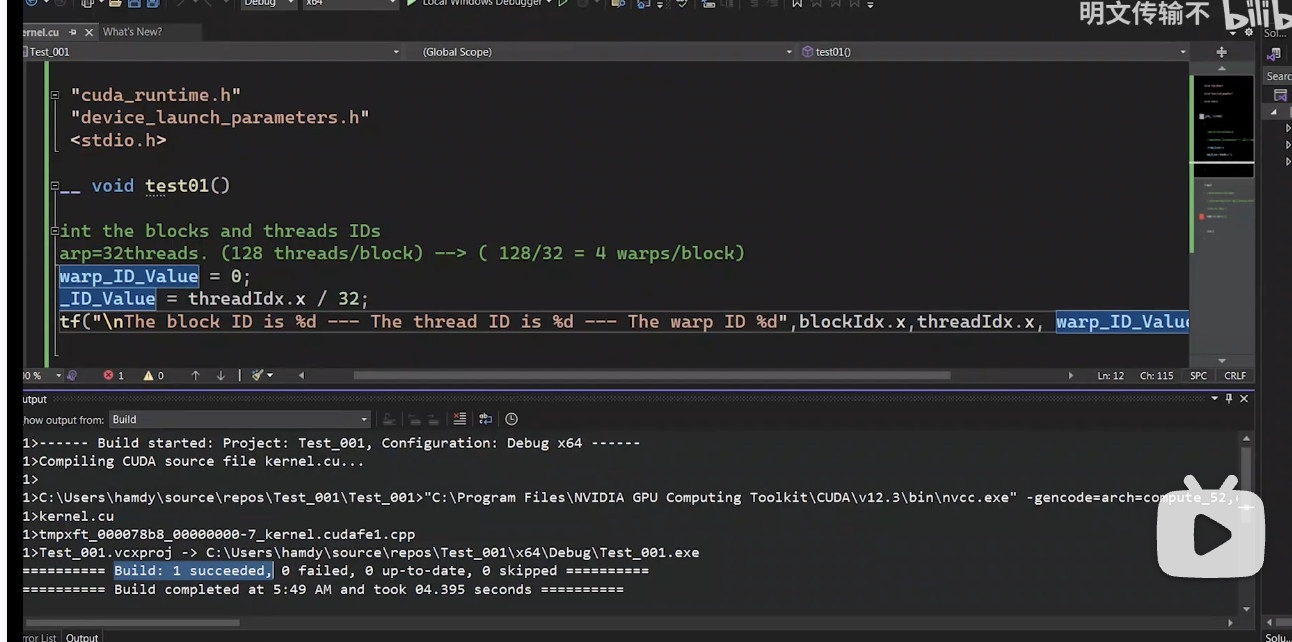
\includegraphics[width=0.75\linewidth]{resources/cuda-073.png}
    \caption{}
    \label{fig:placeholder}
\end{figure}

编译并运行后，可以看到输出结果。首先关注块 ID：当只有 1 个块时，块 ID 始终为 0。线程 ID 从 0 开始（由于并行执行，输出顺序不一定连续），最大值为 127。线程束 ID 从 0 开始，共有 4 个（0、1、2、3），每个线程束包含 32 个线程——线程束 0 包含线程 ID 0 到 31，线程束 3 包含线程 ID 96 到 127。

此时项目中有 1 个块、4 个线程束，每个线程束由 32 个线程组成。计算线程束 ID 还有其他方法（例如使用取模运算），读者可以自行探索。

\subsection{多块场景下的 Warp ID}

将每块线程数改为 64，则每块有 $64 / 32 = 2$ 个线程束。如果同时将块数改为 2，每块的线程束数仍为 2（因为未改变每块线程数），但整个 GPU 上的总线程束数变为 $2 \times 2 = 4$。

\begin{figure}
    \centering
    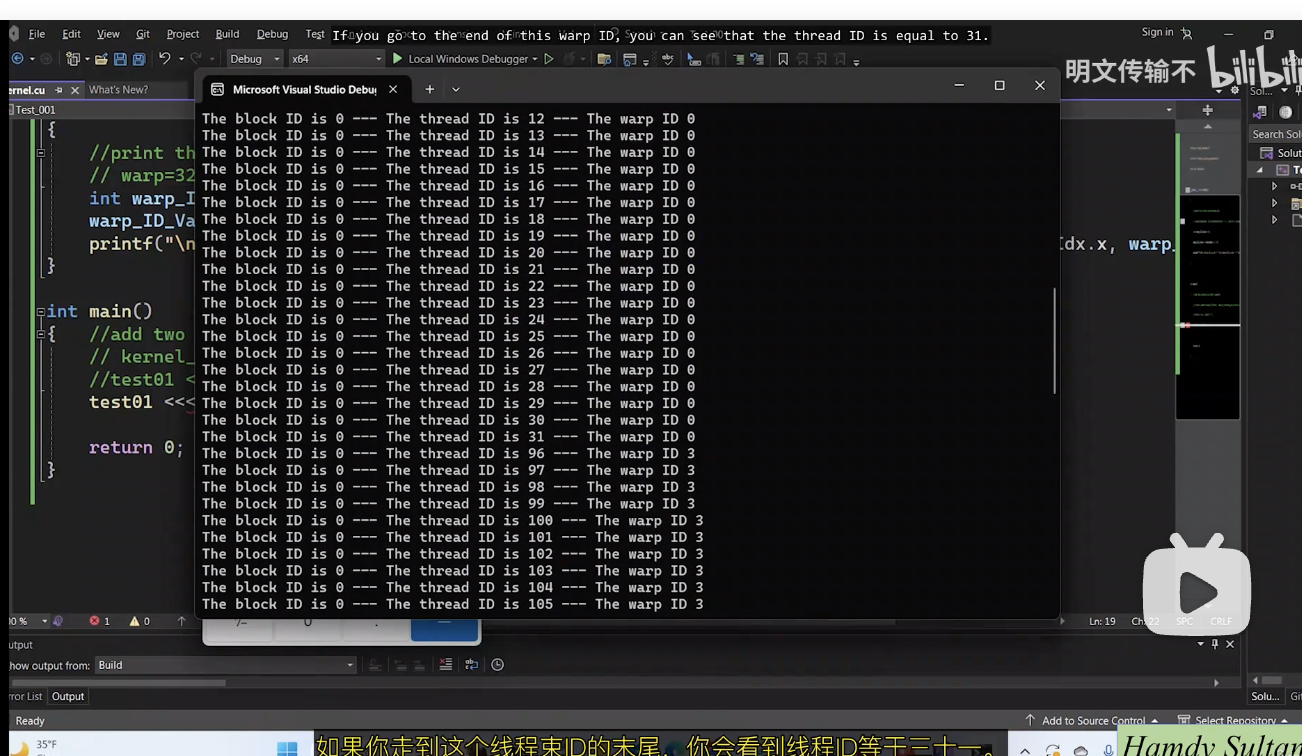
\includegraphics[width=0.75\linewidth]{resources/cuda-074.png}
    \caption{}
    \label{fig:placeholder}
\end{figure}

编译并运行后，输出显示两个块（块 ID 分别为 0 和 1）。关于线程束 ID，可以看到每个块都有线程束 ID 0 和线程束 ID 1。线程束 ID 0 在输出中出现了两次——因为线程束 ID 是\textbf{按块计算的}，而非针对整个 GPU。每个块都有自己独立的线程束编号，因此两个块各自拥有线程束 ID 0 和线程束 ID 1。



\section{CUDA课程项目三：向量加法（Vector Addition）讲解}

欢迎大家。在今天的文章中，我将解释我们的第三个项目——向量加法（VectorAddition）。明确一下，这是向量A，包
含1024个元素，索引范围从0到1023。在这个项目中，我假设我们有两个向量，每个向量包含1024个元素。类似地，我们有
向量B，如图所示。当前的任务是相加这两个向量，结果将存储在向量C中，如图所示。这意味着向量A的第一个元素将与向量B的第一
个元素相加。加法操作将以逐元素的方式在每个元素上进行，结果将存储在C的零位置，也就是C的第一个元素。

\subsection{CPU上的向量加法}

在我们深入GPU代码之前，我想先展示一下这个应用在CPU上的代码。在每次迭代中，我们将向量A和向量B的对应元素相加，并将
结果保存在向量C中。如图所示，这个过程简单地涉及编写一个for循环来遍历所有元素，即1024个元素。以上就是关于在CPU
上运行向量加法的全部内容。但我们需要知道，for循环的迭代将是顺序执行的，而不是并行的。

\begin{figure}
    \centering
    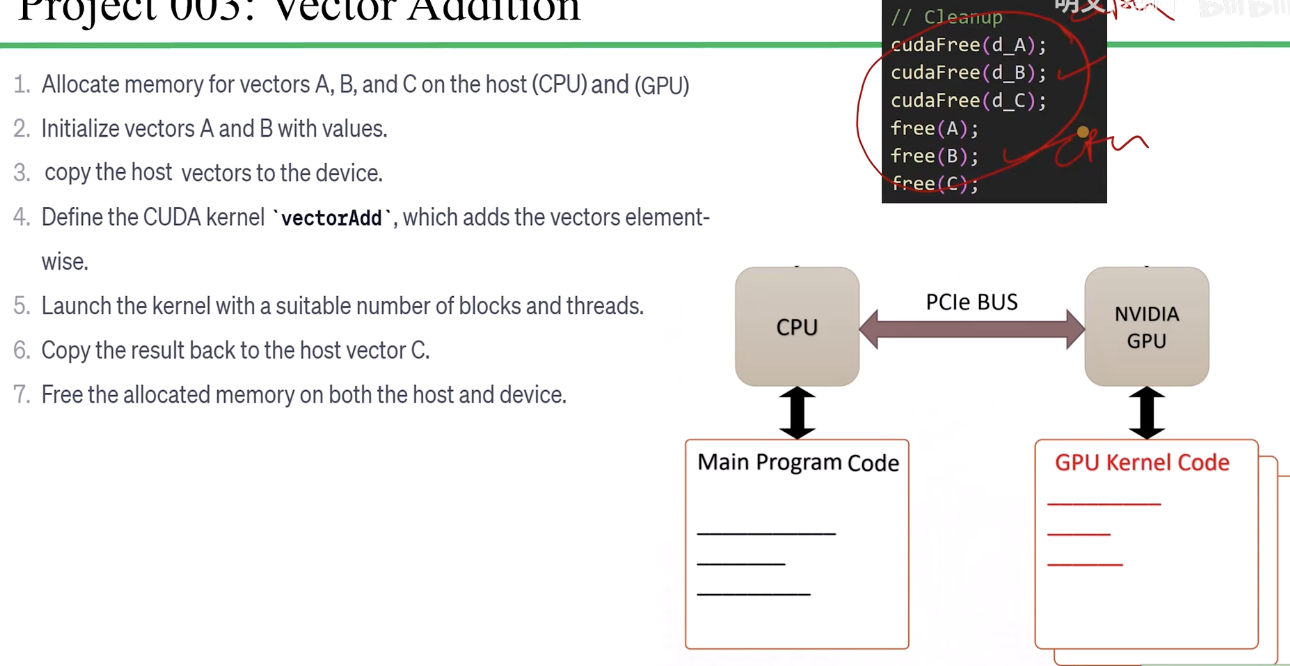
\includegraphics[width=0.75\linewidth]{resources/cuda-075.png}
    \caption{}
    \label{fig:placeholder}
\end{figure}


基于我们之前的讨论，第一步是为我们的GPU应用确定块和线程的数量。让我们探讨这个应用如何在GPU上运行。这里我首先假设只
使用一个块和1024个线程。根据这个信息，我们可以说这里的这个块它的ID将是0，而线程ID的范围将从0到1023。这个选
择使线程数量与每个向量中的元素数量一致。如果你还记得，我说过每个向量有1024个元素，这意味着每个线程ID等于向量中某个
元素的索引。我们只需要再过一分钟就需要这个信息。

很好，现在我们来写出第一个元素的加法操作，仅仅是第一个元素。一个小例子看起来是这样：C的零位置等于A的零位置加上B的零位
置，对吧？考虑到块和线程的ID，在我们的例子中只有一个块，ID是0，这完全没有用。这个模式被复制到第二个元素、第三个元素
，依此类推，覆盖了这些向量中的所有元素。我们不需要块ID，它只是一个零值。然而线程ID表明，正如我们所说，它们等于元素的
索引。这个观察使我们能够有效地为每个线程分配不同的元素。线程ID范围从0到1023，与元素的索引范围相同。例如，线程0可
以与第一个元素对齐，第二个线程可以与第二个元素对齐，以此类推。

\subsection{CUDA核函数实现}

理论部分我们已经讲完了，但现在的问题是这个理论部分如何转化为CUDA代码。实际上这个问题的答案非常简单，实现我们目标所需
的代码很简单，我们这里只需要一个操作——加法操作。这意味着我们将有一个指令或一个操作由多个线程执行。在展示的代码中，声明
了一个名为\texttt{vectorAdd}的GPU内核。然后在接下来的指令中，我们对每个元素执行加法操作。在这个内核
的第一条指令中，我们首先读取线程ID，它的范围从0到1023。因为这里的每个块以及整个GPU的线程总数等于1024。这里
的操作将被执行多次，次数等于线程数。这里的线程ID控制着将要执行加法操作的元素。这1024条指令将被分配给GPU中不同的
核心，以便并行执行。这意味着这条指令将被显式地重写1024次，每次都有一个不同的线程ID。正如这部分提到的，在GPU上相
加这两个向量的内核只需要展示的1到2条指令，无需任何循环。就像在C语言中、像在CPU上运行相同的内核或函数一样。因为在这
里，线程ID会显式地变化以遍历不同的元素，这就是为什么我们在这部分不需要循环。

在我们打开VisualStudio并检查代码及其执行之前，让我们先回顾一下任何CUDA应用的基本步骤。以我们的应用为例，
任何CUDA应用的第一步都是为输入和输出数据分配空间。我们需要为三个向量A、B和C分配内存，对吧？我们必须确保在主机
（CPU）和设备（GPU）上都为这些向量分配了空间。例如，如这三部分所示，这些是实现第一步目的所需的指令。这里我们分配了一些
指针，三个用于CPU分配，另外三个用于GPU分配。然后使用这些指针和这里的\texttt{malloc} 函数，我们在CPU的内存中为三个向量分配所需空间。
类似地，我们使用\texttt{cudaMalloc} 函数在GPU内存中为这些向量分配空间。

如图所示，下一步是初始化输入，我们继续下一步。在我们的例子中，这意味着为向量A和B赋值。因为如果没有先为它们填充值，就无
法执行A和B的加法。这是一个CPU步骤，意味着它将在CPU上执行，而不是GPU。这就是为什么我们使用for循环来执行这一
步，以实现这一步的目的。如图所示，for循环遍历向量A和B的所有元素，然后在每个元素中存储值。

\begin{figure}
    \centering
    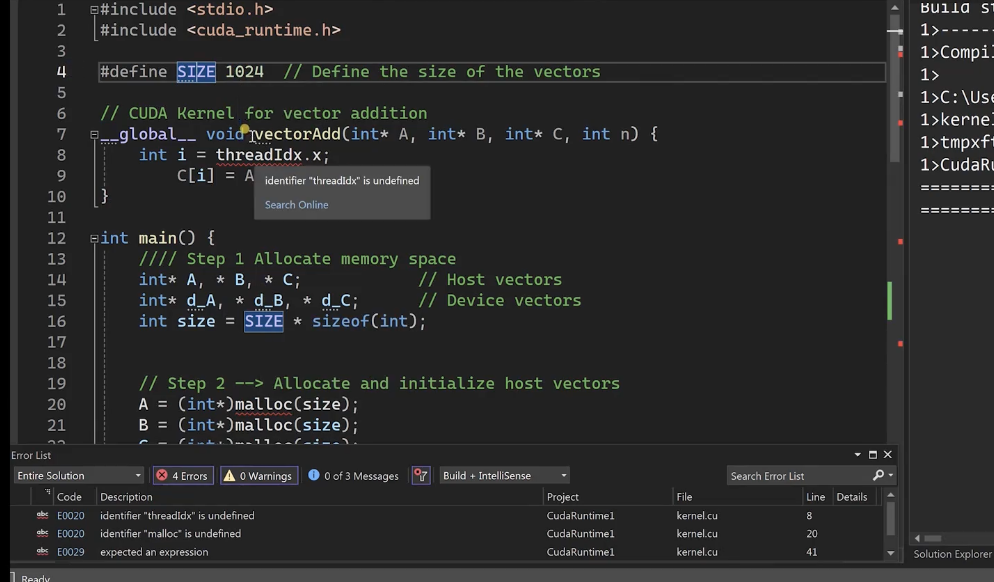
\includegraphics[width=0.75\linewidth]{resources/cuda-076.png}
    \caption{}
    \label{fig:placeholder}
\end{figure}


第三步涉及将这些初始化的A和B值传输到GPU。因为我们的目标是在GPU上执行加法操作，这一步可以通过这2个API或两条指
令实现。有必要将输入数据移动到GPU的内存中。第一个是复制向量A的数据，第二个用于复制向量B的数据。一旦数据进入GPU内
存，我们就可以调用向量加法内核。这可以通过调用GPU内核来实现。如这里的指令所示，这个内核处理A和B的元素以执行加法操作
，并将结果保存在向量C中。正如我们讨论的那样，这条指令包含三个主要部分：内核名称、内核配置（或块和线程的数量），以及最后
是这个内核的输入参数。这就是实现这一点的指令。


在结果安全存储在GPU内存中之后，下一步是将它们传输回CPU内存。在那里你可以打印它们，或将它们发送到另一个阶段，或发送
到另一个GPU内核进行进一步计算等等。它只是一个内存复制操作，但这次它的配置是从GPU、从设备到主机、从GPU到CPU。
如图所示。这个过程的最后一步是释放之前在CPU和GPU上分配的内存空间。这确保了高效的资源管理，并避免内存泄漏。

\subsection{完整代码解析}

如你所见，我以每个向量的大小开始这段代码，这就是我们项目的代码，大小等于1024个元素。每当我们需要改变应用中向量的大小
时，我们所要做的就是来到这里并更改这个值。这就是为什么我们需要在应用开始时预定义大小。然后我们有GPU内核，我们知道这是
一个GPU内核，而不是CPU函数，因为这里的这个部分\texttt{\_\_global\_\_}，这意味着这一部分或这
个内核或这些指令将在GPU端执行，而不是在CPU端。内核名称是\texttt{vectorAdd}，如你所见，它接受四个
值。如我们所看到的，向量A、向量B这些是输入，向量C这是输出或我们将存储结果的地方。然后我们还有另一个变量N，实际上这个
变量等于大小，它将会是1024。但我今天跳过它，在下一个文章中，我将在另一个文章中解释N变量背后所有的技巧。因为我们需要
在这里使用它，但不是今天。

然后我们有这两条指令，实际上我们可以将它们合并为一条指令。我们需要做的就是复制这部分并放在这里第一条指令。但我不想这样做
，因为我在为你们准备更复杂的应用。这里是读取线程ID，正如我们所说，我们有1024个线程，这个将包含线程ID的值，不同的
线程ID将用于遍历这些向量中的所有元素。这里的线程ID将从0到1023。明白吗？这就是GPU内核，它非常简单。

然后这是主函数的开始。如你所见，第一步是分配一些指针以供使用，下一步是在CPU端和GPU端分配空间。例如这三个向量，如你
所见，将用于在CPU内存上为三个向量分配空间，用于向量A、向量B和向量C。如你所见，我们使用\texttt
{malloc}函数来分配这些空间。但是记住，这是每个向量的大小，如你所见，这个大小将被使用。不要忘记我们在这里预定义
了大小，而这个大小并不正好是1024，因为我们乘以了整数值的大小（\texttt{sizeof(int)}）， 这就是我
们使用\texttt{malloc} 函数的方式。总之你需要具备非常简单的C语言背景才能理解这里的一切。

然后我们使用这里的另外三个指针来在GPU内存上分配空间，而不是CPU。这里这是针对CPU的对吧？但这三个指令是为在GPU
内存上分配三个向量所需的空间。如你所见，这是第一个向量，从这个部分；第二个向量；第三个向量。它们都使用相同的大小。

下一步是初始化向量A和向量B。我们不会初始化向量C，因为这是我们将要存储结果的地方，我们不需要用任何值初始化它。这里我们
使用一个for循环来遍历向量A和向量B内的所有元素，我们只是存储一些值。这个for循环的结束条件在这里是1024。如你所
见，例如在A中我们存储I的值，I从0到1024。第一个元素将等于0，第二个元素将等于1，最后一个元素将等于1023。以此
类推。如果I等于0，B的值将等于1023。B也是一样，但它的值等于1024减去I值。这非常简单，没什么难的，但无论如何，
我们不需要关注值本身。你可以用任何你想要的值来初始化A和B。

然后一旦我们初始化了A的值和向量B的值，我们需要将这些值从CPU传输到GPU。因为这里的A和B在CPU端，不在GPU端。
如果你记得，A和B是CPU的，\texttt{d\_A}、\texttt{d\_B}是GPU端的。我们需要做的就是使用这
个函数\texttt{cudaMemcpy}，意思是CUDA的内存复制操作。我们将要从主机复制到设备，主机指的是CPU，
设备指的是GPU，这就是这条指令的用法。我们将要从指令A复制到指令\texttt{d\_A}，这是从CPU，这是到GPU
。我们要复制的数据量等于这个大小。向量B也是如此，如你所见，我们将移动数据，大小等于这个值，从CPU到GPU，从变量B到
GPU上的变量\texttt{d\_B}。我们不需要复制向量C，因为向量C将存储结果。

一旦你通过这两个指令或API将数据放入GPU内存，你需要做的就是执行向量加法内核 \texttt{vectorAdd}内
核。我们在这里启动，我们调用 \texttt{vectorAdd}内核，它将执行这里的这两条指令。我们将使用的配置是我们
的一个块，每个块1024个线程。并且我们将发送或说明这个内核将使用向量A、向量B、向量C，如你所见，以及所有这些向量的大
小作为输入。一旦你调用这个函数，执行将从CPU端转移到GPU端。它会来到这里并执行所有线程，这意味着对所有元素执行加法操
作，并将结果存储在C中。

一旦我们在C中有了结果，这一步之后，我们需要做的就是将数据从GPU内存复制回CPU内存。如你所见，我们将结果复制回主机，
只是为了将这部分与这部分进行比较。\texttt{cudaMemcpyDeviceToHost}，这里我们
有\texttt{HostToDevice}。如你所见，我们要传输或移动的数据量等于这个大小，并且我们从GPU向量移动到
CP U向量 。我需要你注意这里的顺序，这里从GPU到CPU。

一旦我们在向量C上有了数据，而向量C在CPU端，我们就可以打印结果C值。我在这里使用for循环遍历所有元素并打印A、B和
C值。如你所见，A加B等于C。一旦你打印完结果，你需要释放两端所有分配的空间，CPU端和GPU端。如你所见，这里我使
用\texttt{cudaFree} 释放GPU的内存，CPU端也是一样，但只使用一个叫 \texttt{free}的函
数。 正如我告诉你的，它们非常相似，这里的 \texttt{free}，这里的\texttt{cudaFree}。但是因
为这将释放GPU上的空间，我们在这里使用了CUDA术语。

如你所见，这些是主要步骤。我们需要做的就是来到这里并构建，以确保没有任何错误。看这里，这个部分我从下面移到了右边。如你所
见，我们的应用编译正确。如你所见，构建成功，所以我们没有任何失败。我们现在需要做的就是运行这个应用。如你所见，我们正在打
印值，因为所有操作都已经执行完毕了。这些值来自这个部分，来自这个for循环，明白吗？这意味着之前所有的步骤都已正确执行。
是的，这些就是结果。为了让它更简单，就在这里用比如32个值，然后编译并运行。让我们放大看看这些值。这是第一个值，A的第一
个元素加上B的第一个元素，这就是结果。如果你还记得这里的初始化过程，这个部分我们用相同的值从0到32或31初始化了A向量
，而B向量一开始以32结束。这些是A的值，从零开始到31结束。这就是初始化过程，你可以选择任何其他值，看看它们是否正确。
我们的结果给出了正确的值。例如，23加9等于32。

我们现在需要做的就是改变块和线程的数量。但我要在这个文章中跳过它，在另一个文章中再做，因为我不想让这个文章太长。请跟进本
课程的所有文章，以便能够理解一切。今天就到这里，下个文章见。


\section{CUDA 编程教程：向量加法扩展与 GPU 利用率优化}

本章将继续讨论上一个项目。在上一个项目中，处理了两个向量，每个向量包含 1024 个元素，因此选择了一个块和 1024 个线程。本章计划将向量大小扩展到 2048。

\subsection{问题提出与硬件限制}

问题来了：是否可能用一个块来运行 2048 个线程？要回答这个问题，需要查阅白皮书。在 Ampere 架构的情况下，白皮书给出了明确的答案：这是不可能的。每个块的最大线程数是 1024。

\begin{figure}
    \centering
    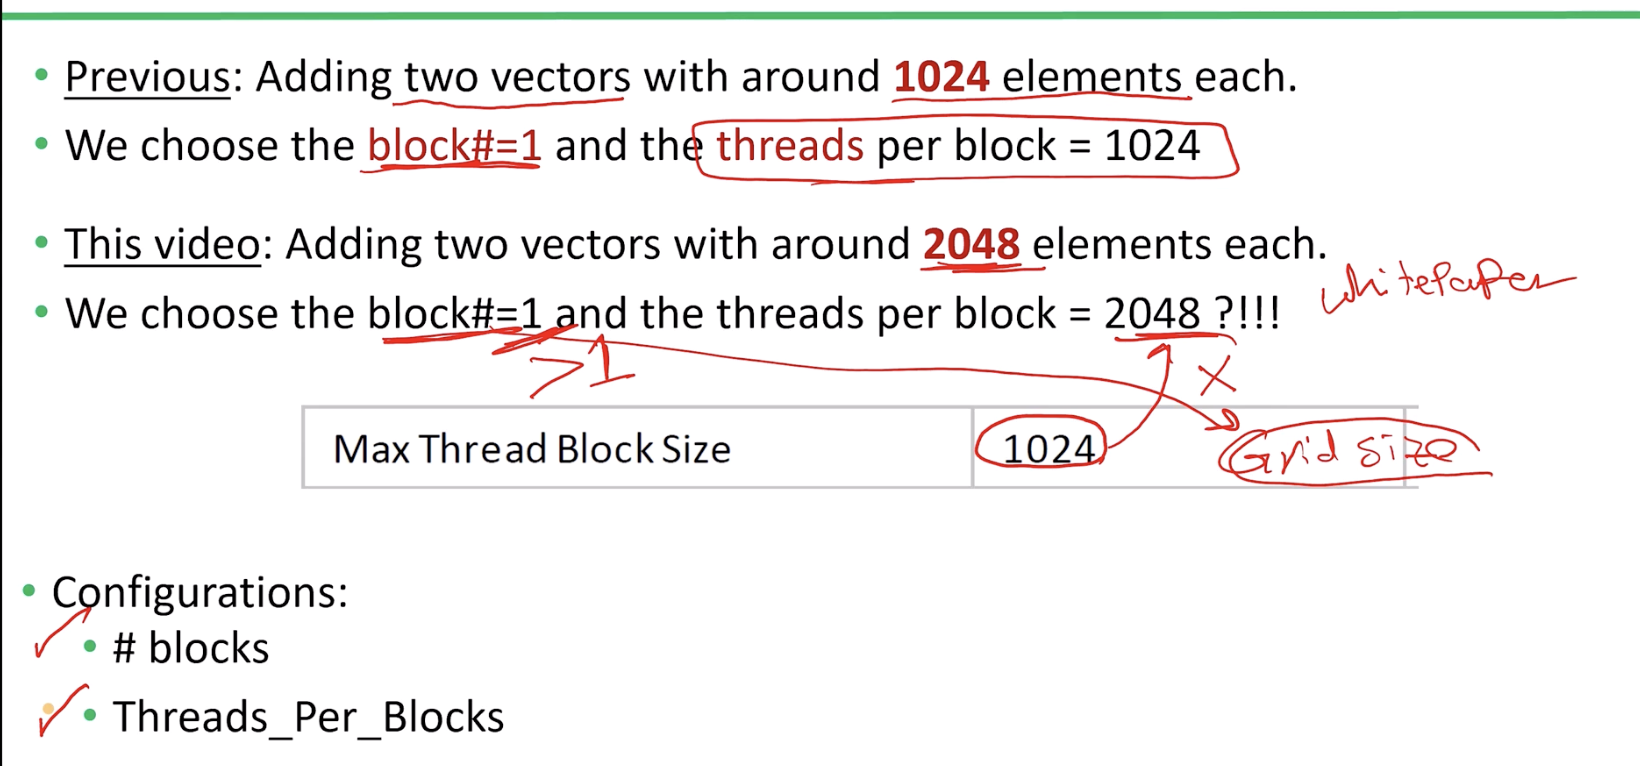
\includegraphics[width=0.75\linewidth]{resources/cuda-077.png}
    \caption{}
    \label{fig:placeholder}
\end{figure}


\subsection{解决方案：调整网格配置}

为了解决这个问题，需要调整网格大小，即增加项目中的块数。与上一个项目使用一个块不同，这里需要使用多个块。可以灵活地决定块的数量以及每个块应包含的线程数，但必须遵循的关键规则是：确保应用程序中的总线程数与向量中的最大元素数相匹配。这意味着如果块数增加（这里的块数指的是网格大小），每个块的线程数必须相应减少，以确保总线程数保持在 2048。

这种情况确实会引起需要关注的性能问题，但将从一个简单的方法开始，只使用两个块，每个块配备 1024 个线程。性能影响将在后续阶段深入探讨。

\subsection{索引映射原理}

如图所示，有一个 2048 个元素的向量。方法是将这个向量分成两部分，每个部分由各自的块来执行。有一个 ID 为 0 的块用于第一部分，一个 ID 为 1 的块用于第二部分。第一部分有 1024 个线程，每个线程专门用于在单个向量元素上执行加法操作，这些线程的 ID 范围从 0 到 1023。这个配置在第二部分中镜像，即第二部分中的线程 ID 范围也是从 0 到 1023。

现在必须将两个部分中的块 ID 和线程 ID 与向量索引对齐，以确保每个向量索引都与一个专用线程匹配来执行加法操作。对于第一部分，这很简单，因为线程 ID 与向量索引相同。然而在第二部分中，向量的索引从 1024 开始，一直到 2047，而线程 ID 仍然从 0 开始，在 1023 结束。

为了解决这个问题，特别是在第二部分，应用以下等式：向量中任何元素的索引计算为\textbf{线程 ID 加上块 ID 乘以每个块的总线程数}。举个例子来验证这个等式对两个部分都有效。

\begin{figure}
    \centering
    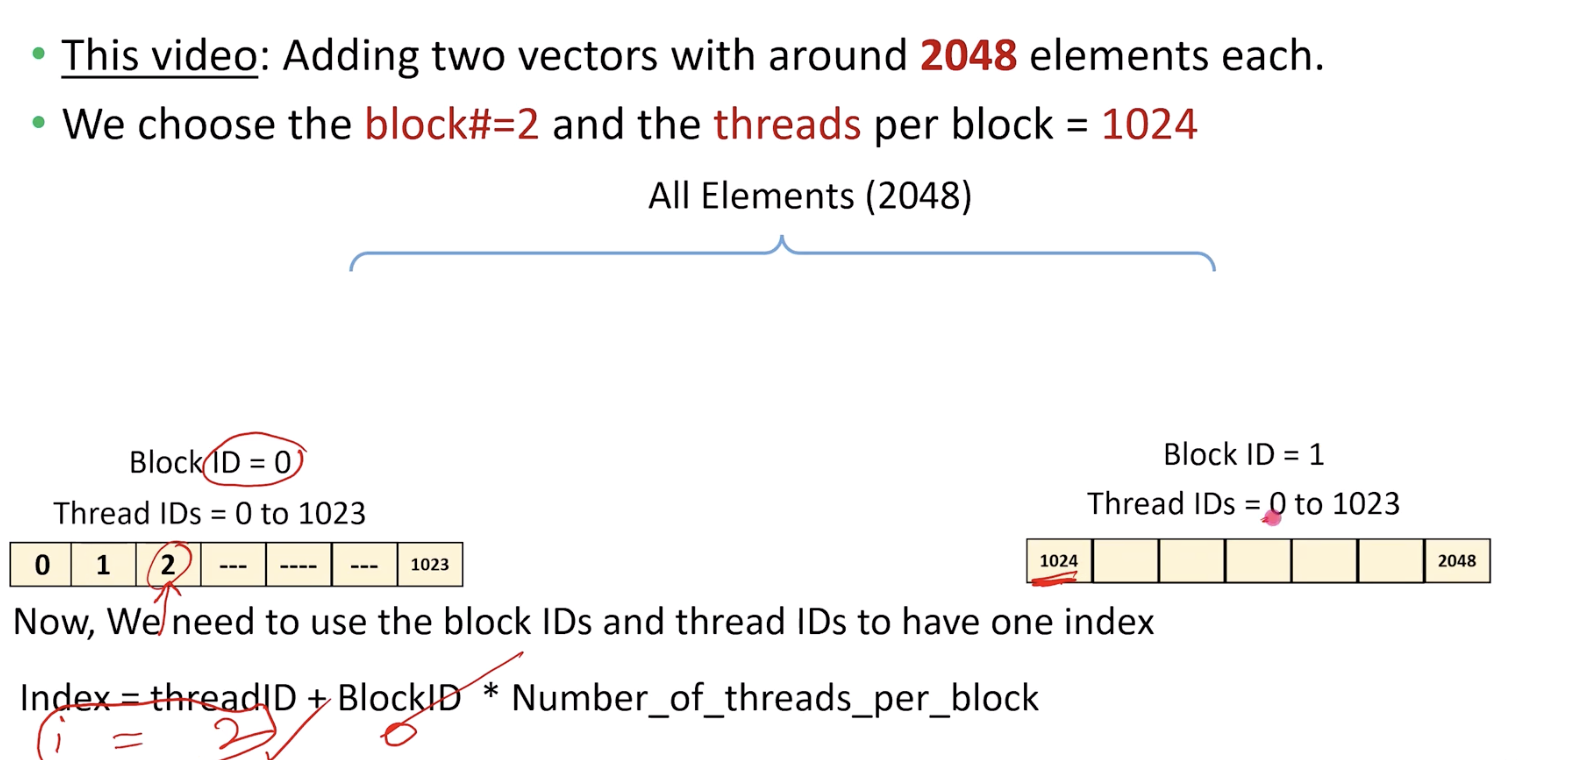
\includegraphics[width=0.75\linewidth]{resources/cuda-078.png}
    \caption{}
    \label{fig:placeholder}
\end{figure}


以向量中的第三个元素为例，块 ID 为 0、线程 ID 为 2。将这些值代入等式，计算结果为索引 2，这是正确的。另一方面，对于后半部分的第一个元素，其线程 ID 为 0，块 ID 为 1，得到索引 1024，这也是准确的。这个等式对两个部分都适用。

需要强调的是，这个等式至关重要，并将继续是 CUDA 编程工作的重要组成部分。

\subsection{代码实现}

请注意，这个等式在编码方面与上一章中的项目非常相似。主要任务涉及直接在核函数中应用索引等式。在这里，将替换这条指令，写成：

\begin{lstlisting}[language=C++,basicstyle=\ttfamily\small]
index = threadIdx.x + blockIdx.x * blockDim.x;
\end{lstlisting}

这里的 \texttt{blockDim.x} 指的是 X 方向上每个块的最大线程数。别忘了在这里将向量大小从 1024 改为 2048。同时需要修改应用程序配置，在这条指令中，需要将这个值从 1 改为 2，以反映对两个块的需求。

在满足其他要求后，现在是编译和运行项目的时候了，并确保每个块中有 1024 个线程。如图所示，项目运行良好，这些就是结果：A 的第一个元素加 B 的第一个元素将存储在 C 向量的第一个位置。

\subsection{GPU 利用率分析}

有两个问题需要探讨，同样的规则适用于 2048 个元素。

\subsubsection{问题一：SM 的使用数量}

第一个问题：基于选择的配置，有多少个 SM（流式多处理器）将被用来执行这个项目？提出这个问题是为了鼓励时刻留意设置对所分配的硬件资源的影响。这将如何影响分配的硬件资源？例如，在这个应用程序中，选择了两个块，每个块 1024 个线程，这将如何影响应用程序的性能？

在回答这个问题时，有必要参考之前提供的图片。如图所示，并且如前所述，一个线程在 GPU 核心上运行（这里的核心是 GPU 中最小的硬件单元，这是软件和硬件中的第二层级）；块在整个 SM 上运行；网格在整个 GPU 上执行。线程束（Warp）在 SM 分区上执行，因为每个 SM 包含多个分区。

据此，在应用程序中，有两个块，这表明只有 2 个 SM 将参与执行这个应用程序。这个衡量标准被称为\textbf{GPU 利用率}。假设拥有 Ampere 架构的 A100 GPU，这个 GPU 拥有 108 个 SM，那么 GPU 利用率将低于总可用 SM 的 2\%。因为只使用了 2 个 SM，而剩下的 106 个 SM 处于空闲状态，没有工作。GPU 利用率是 GPU 性能的一个关键指标。在这个例子中，GPU 利用率极低。

\begin{figure}
    \centering
    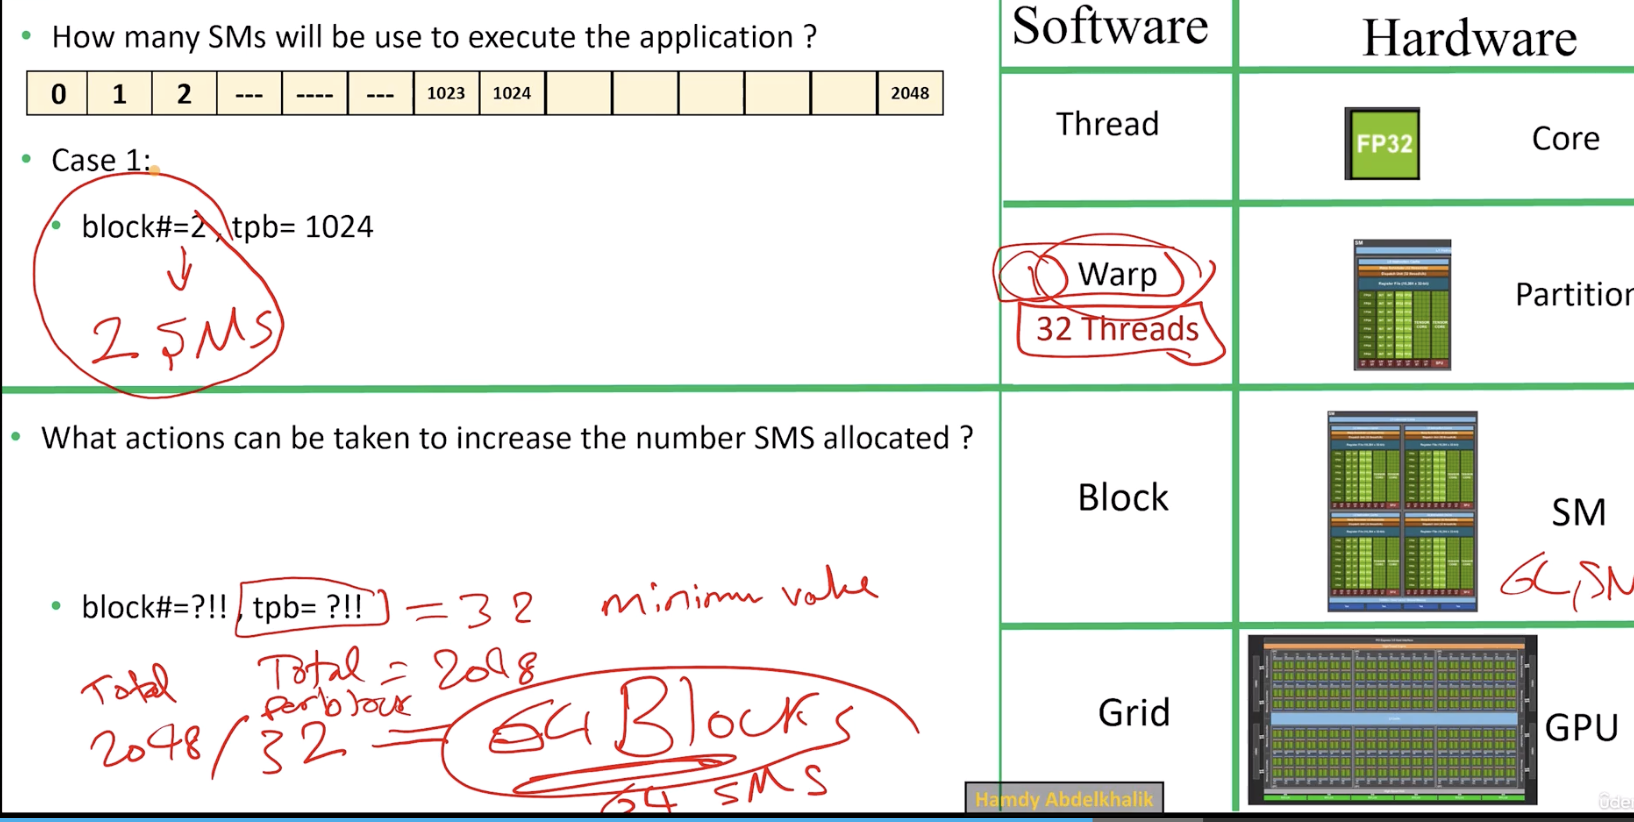
\includegraphics[width=0.75\linewidth]{resources/cuda-079.png}
    \caption{}
    \label{fig:placeholder}
\end{figure}


\subsubsection{问题二：提高 GPU 利用率的措施}

现在看第二个问题：可以采取哪些措施来增加为运行此应用程序分配的 SM 数量？这里希望在不增加向量大小的情况下回答这个问题。这个问题也意味着如何提高 GPU 利用率。

这非常简单：如果能使用更多的 SM，那么就在使用更多的资源，这意味着提高了 GPU 利用率。应该增加块的数量，并且如果可能，应该增加每个块的线程数。在这种特定情况下，同时增加两者不是一个选项，因为总线程数需要与向量中的元素数量匹配。拥有比向量中元素总数更多的线程会引发一个问题：这些额外的线程将执行什么操作？

为了保持总线程数为 2048，策略是增加块数，同时减少每个块的线程数。应该使用的最小每块线程数等于 32，这相当于一个线程束（Warp）的大小，也就是在任何块中可以使用的最小线程数。需要将 2048 个线程除以 32，得到在此应用程序中可以使用的总块数：$2048 \div 32 = 64$ 个块。

这个配置意味着将使用该 GPU（即 A100 GPU）的 64 个 SM。与第一种情况中只有两个块和两个 SM 相比，这里有 64 个块将在 64 个 SM 上运行。

\subsection{执行时间测量}

可以使用两种不同的方法来计算执行时间。为了验证工作并了解这将如何影响应用程序性能，需要测量两种不同场景下的执行时间。一种方法是利用 CUDA 的内置 API，另一种可以使用分析器（Profiler）。本章将采用 CUDA API 方法。这里的分析器指的是 NVIDIA 的诊断工具，如 Nsight Systems 或 Nsight Compute。

现在打开 Visual Studio 看看代码。如图所示，添加了几行专门用于测量执行时间的代码。这个过程的第一条指令是声明两个变量 \texttt{start} 和 \texttt{stop}。之后应用一个名为 \texttt{cudaEventCreate} 的函数。这两个变量是由 \texttt{cudaEvent\_t} 类型声明的，这个函数准备这些变量以供使用，类似于初始化。然后使用 \texttt{cudaEventRecord} 函数来开始记录时间，在这里将初始时间或开始时间存储在 \texttt{start} 变量中。

在这条指令中，正在 GPU 上执行核函数。正如之前讨论的那样，一旦执行完成，再次记录时间并将值存储在 \texttt{stop} 变量中。下一步是使用 \texttt{cudaEventElapsedTime} 函数，从 \texttt{stop} 值中减去 \texttt{start} 值。这个计算提供了以毫秒（ms）为单位的执行时间。

现在编译并运行项目。如图所示，这就是执行时间，请注意这个值。然而再运行一次，读取这个值并记在脑子里。现在再次运行——这印证了对这种计时方法的保留意见。正如观察到的，执行时间可能因每次运行而异。这种方法缺乏精确性，使用分析器是更好的选择。

\subsection{性能对比与总结}

总之，现在回到代码并调整块数和每块线程数。可以在这里选择 64 个块，每个块有 32 个线程，这是第二种场景。再次运行应用程序后，如图所示，可以轻易观察到当前的执行时间比第一种情况减少了。

现在应该清楚了。回到演示幻灯片，更深入地探讨这个话题。

在第一种场景中，有两个块，在总共 108 个可用 SM 中的两个上并行运行。这里需要记住，这些块中的每一个都配置了 1024 个线程，而 1024 个线程是在一个块中可以使用的最大线程数。这意味着这里的块尺寸非常大。

在第二种场景中，有 64 个块在 64 个 SM 上并行运行。与第一种场景相比，这里的块明显更小，每个块包含 32 个线程，而第一种场景中是 1024 个线程。

这里有一个问题：看看第一种情况或第二种情况下可用的 SM，告诉我在任何这些 SM 上将要执行的最大块数是多少。在第一种情况下，第一个 SM 上面将要执行的最大块数是多少？第二个 SM 呢？无论如何，可以说每个 SM 的最大块数等于 1。

再看第二种情况回答同样的问题。有 64 个块，每个 SM 将只执行一个块，这些块将分布在 64 个 SM 上。再次强调，每个 SM 的最大块数等于 1 个块。别忘了这两种情况下的块将并行执行，而不是顺序执行。这意味着执行时间将根据块的大小来计算。如果第二种情况下的块更小，第一种情况下的块更大，那么第二种情况将比第一种情况执行得更快。

希望现在明白了应用程序配置如何影响其性能。本章到此结束。



\section{大规模向量加法：内存限制与分块处理策略}

\subsection{引言：从中小规模到超大规模向量}

在之前的项目中，创建了 CUDA 程序来实现两个向量的加法，但那些向量的规模较小。本章将涵盖相同的应用程序——向量加法，但专注于尺寸大得多的向量。这个任务不会像之前的项目那样直截了当，将更加复杂。很可能会遇到几个挑战，本章将在遇到每一个挑战或问题时指出它，并提供相应的解决方案。

在上一个项目中，向量的大小是 2048 个元素，分配了两个线程块（block），每个块包含 1024 个线程。本章将把向量大小增加到超过 4 亿个元素。

当前的向量大小设定为 $1024 \times 432 \times 1024$，确实超过了 4 亿个元素。

转到启动核函数（Kernel）的指令。在这条指令中，使用每块 1024 个线程。为了处理所有这些元素，必须调整应用程序中的主要配置，即块数（Grid Size）和每块线程数（Block Size）。这代表了 GPU 的最大限制。对于网格大小（即块的数量），使用 $1024 \times 432$ 个块。这段代码中的其他所有内容都与之前的项目类似，不编辑其他部分。这两个配置的乘积应等于每个向量中的元素总数。

现在编译并运行。由于在处理很大的向量尺寸，这个应用程序的执行将花费一些时间。如所示，一切正常，结果显示如图。可以在这里选择任意一行，测试 $A + B$ 是否等于 $C$ 的值。无论是编译还是运行应用程序，都没有出现编译错误或运行时错误。

\subsection{挑战一：超出主机内存限制}

进一步增加向量尺寸时，问题出现了。到向量大小定义处复查一下，将 432 替换为 1024。现在每个向量都有超过 10 亿个元素。编译后发现没有任何编译错误。运行应用程序，如图所示，代码未能正确运行。代码中用于验证结果的 for 循环输出没有再显示在终端上。此外，可以注意到，如果错误码为零，则表示没有错误；如果是非零数字，则表示遇到了运行时错误。该应用程序中没有编译错误。

需要思考一下这个问题：为什么在这个应用程序中遇到了错误？可能的原因是什么？


\begin{figure}
    \centering
    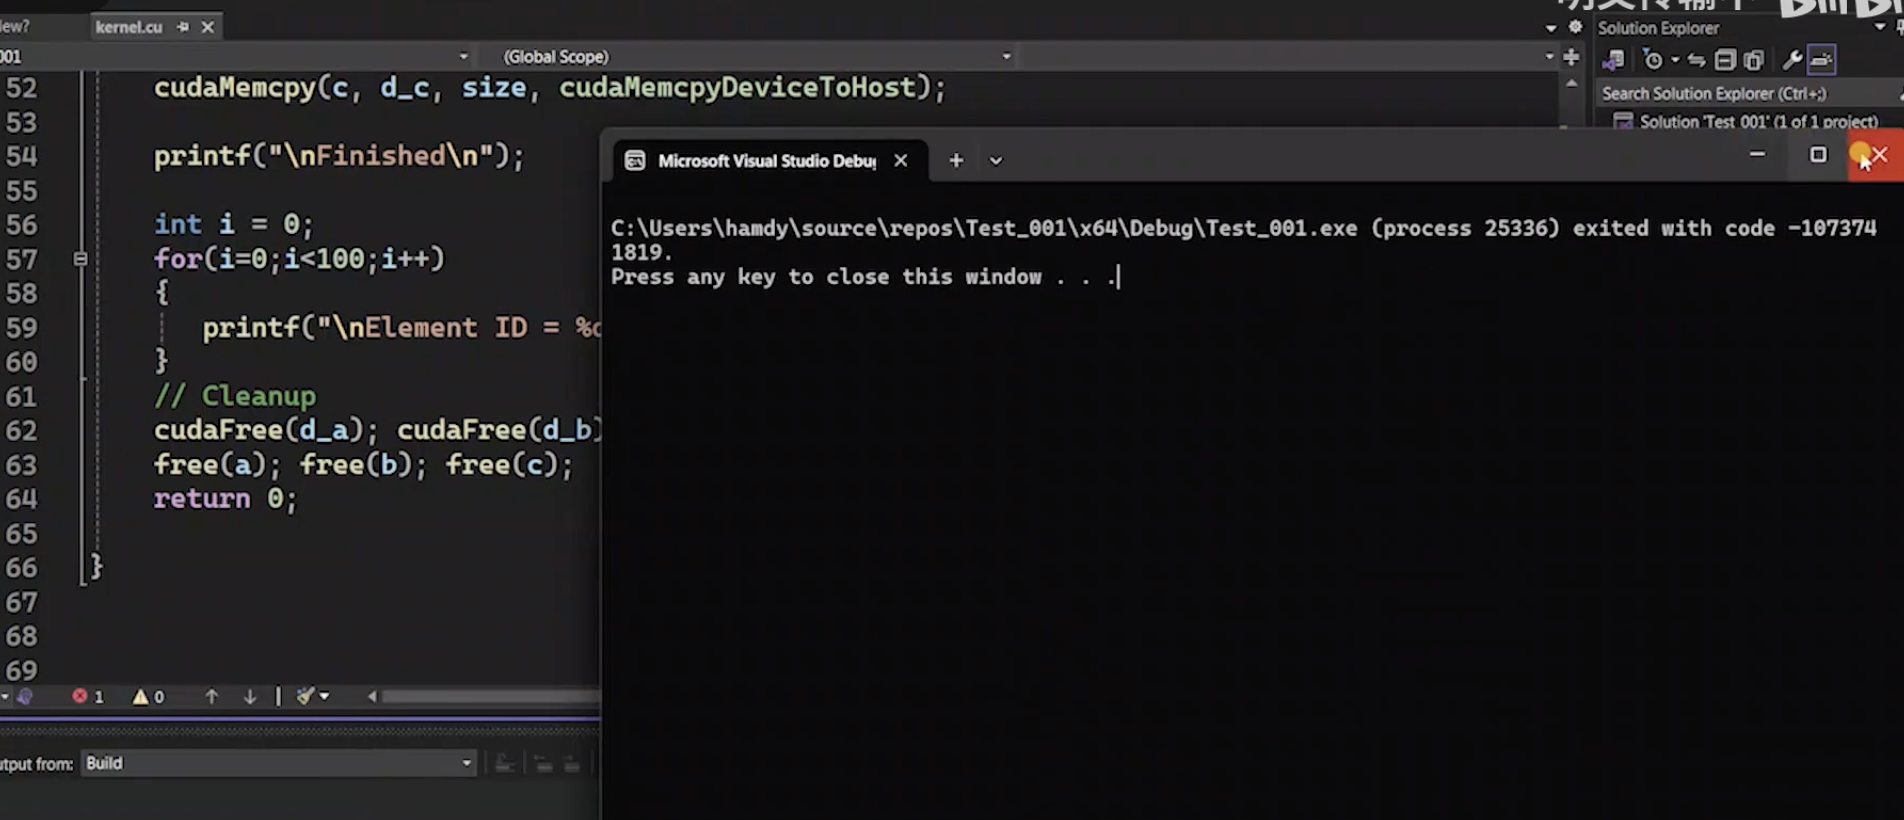
\includegraphics[width=0.75\linewidth]{resources/cuda-080.png}
    \caption{}
    \label{fig:placeholder}
\end{figure}


\subsection{调试策略：使用 printf 定位问题}

下面提供解决方案。有很多调试策略可以找到确切的问题所在。在这种情况下，最有效的调试技巧之一是使用 \texttt{printf} 函数。在应用程序的不同位置放置许多 \texttt{printf} 指令，然后运行应用程序，利用终端上的输出来定位有问题的代码行。

例如，在开头写第一个 \texttt{printf("hello 00\textbackslash n");}，然后将这条指令复制到不同的位置，并依次标记为 01、02 等。为什么需要在不同的位置放置 \texttt{printf} 指令？因为需要识别错误发生的具体位置。这与语法错误不同——如果移除一个分号，编译器会明确告知问题所在。但在当前情况下，遇到的是运行时错误而非编译错误。

编译成功后，看到终端打印了 "hello 00" 和 "hello 01"，但 "hello 02" 没有打印。这意味着错误发生在 "hello 01" 之后、"hello 02" 之前。结合上下文，发现 GPU 内存分配（\texttt{cudaMalloc}）本身没有报错，问题出在 CPU 端的主机内存分配上。

\subsection{根本原因分析}

为了理解这一点，查看 RAM（主机内存）中的可用空间。假设计算机总共有 16 GB RAM，当前已使用约 10 GB，剩余约 6 GB 可用空间。回到代码，当运行应用程序时，流程是为向量 A 分配空间并初始化，然后为 B 分配并初始化，最后为 C 分配空间。

当向量维度设置为 $1024 \times 1024 \times 1024$ 时，单个向量的元素数量为 $1,073,741,824$。由于每个整数元素占 4 字节，单个向量的大小为：
\[\frac{1024 \times 1024 \times 1024 \times 4 \text{Bytes}}{1024^3} = 4 \text{ GB}\]要存储三个向量（A、B、C），总共需要 12 GB 主机内存，而计算机上没有这么多可用空间。这就是导致运行时失败的根本原因。虽然 GPU 显存可能足够，但 \texttt{malloc} 在主机端分配内存时失败了。

\subsection{解决方案：数据分块（Chunking）处理}

解决此问题的方案是将每个向量分成小块（chunks）。具体使用多少块取决于可用内存。假设有 4 至 5 GB 可用空间，每个数据块的大小应小于此限制。

例如，将维度中的 1024 替换为 128。这意味着将把每个向量分成 8 块，因为 $1024 / 128 = 8$。使用这个"块大小"（chunk size）来分割向量。处理流程如下：取 A 的第一块和 B 的第一块相加，将结果存入 C 的第一块；完成后释放这些临时缓冲区占用的内存；然后转到向量的第二部分，依此类推，直到处理完所有部分。

\subsection{分块代码实现逻辑}

以下是修改后的核心逻辑说明：

\begin{enumerate}
    \item \textbf{参数定义}：定义总大小（total size）、数据块大小（chunk size）以及块数量（num chunks = total size / chunk size）。线程块大小仍保持为每块 1024 个线程。
    \item \textbf{核函数}：GPU 核函数和初始化函数无需修改，仅需传入数据块指针而非完整向量指针。
    \item \textbf{内存分配}：不再为整个向量分配空间，而是仅为当前数据块分配空间。使用 \texttt{malloc(chunk\_size * sizeof(int))} 为 \texttt{chunk\_A}、\texttt{chunk\_B}、\texttt{chunk\_C} 分配主机内存。GPU 端同样只分配数据块大小的显存。
    \item \textbf{迭代处理}：使用 for 循环遍历所有数据块。在每次迭代中：
    \begin{itemize}
        \item 计算当前偏移量（offset = i * chunk\_size）；
        \item 初始化或加载当前块的 A 和 B 数据；
        \item 使用 \texttt{cudaMemcpy} 将数据块拷贝到 GPU；
        \item 执行核函数进行向量加法；
        \item 使用 \texttt{cudaMemcpy} 将结果从 GPU 拷回主机的 \texttt{chunk\_C}；
        \item 验证或输出当前块的结果；
        \item 释放当前块的主机和设备内存，为下一次迭代做准备。
    \end{itemize}
\end{enumerate}

\subsection{验证与结果}

编译并运行修改后的代码。编译成功。运行时，终端打印了每个数据块的偏移量：0、128、256……直到第 8 个块。这证实了循环正确执行了 8 次迭代。

观察内存使用情况，仅使用了约 1 GB 左右的额外空间，因为只为两个数据块（A 和 B 的当前块）分配了空间，而不是三个完整的向量。当程序完成并释放内存后，可用空间恢复到了初始水平。

最终结果是正确的，例如 $13 + 77 = 90$ 等验证均通过。这就是本章讨论的第一个挑战及其完整的解决方案：通过数据分块技术突破主机内存限制，实现超大规模向量运算。



\section{CUDA运行时API详解与设备属性查询}

大家好，在今天的文章中我将解释CUDA运行时API（RuntimeAPI）。CUDA运行时API为CUDA提供了一个高级
接口，它使开发者能够高效地利用NVIDIA GPU的能力来完成广泛的计算任务。这些API简化了管理GPU设备、内存分配以及
执行并行内核的过程。

运行时API可供程序员用来开发优化或运行GPU加速的应用程序。这种方法是一个省时的替代方案，无需阅读GPU白皮书中详细的
文档。例如，无需深入研究白皮书来查找设备限制和约束。就像我们在前一节中解释的那样，例如每个块的最大线程数，这些API提供
了函数，允许你直接从GPU查询那个值。

让我们来查看这个专门用于运行时API函数的网页。如这个网页所示，我们有数十个函数，涵盖设备管理（例如这个函数）、内存处理
（比如这一个）以及异步计算。如果你想从运行时API中找到任何函数，你需要来到这个网页。

\subsection{核心函数：cudaGetDeviceProperties}

\begin{figure}
    \centering
    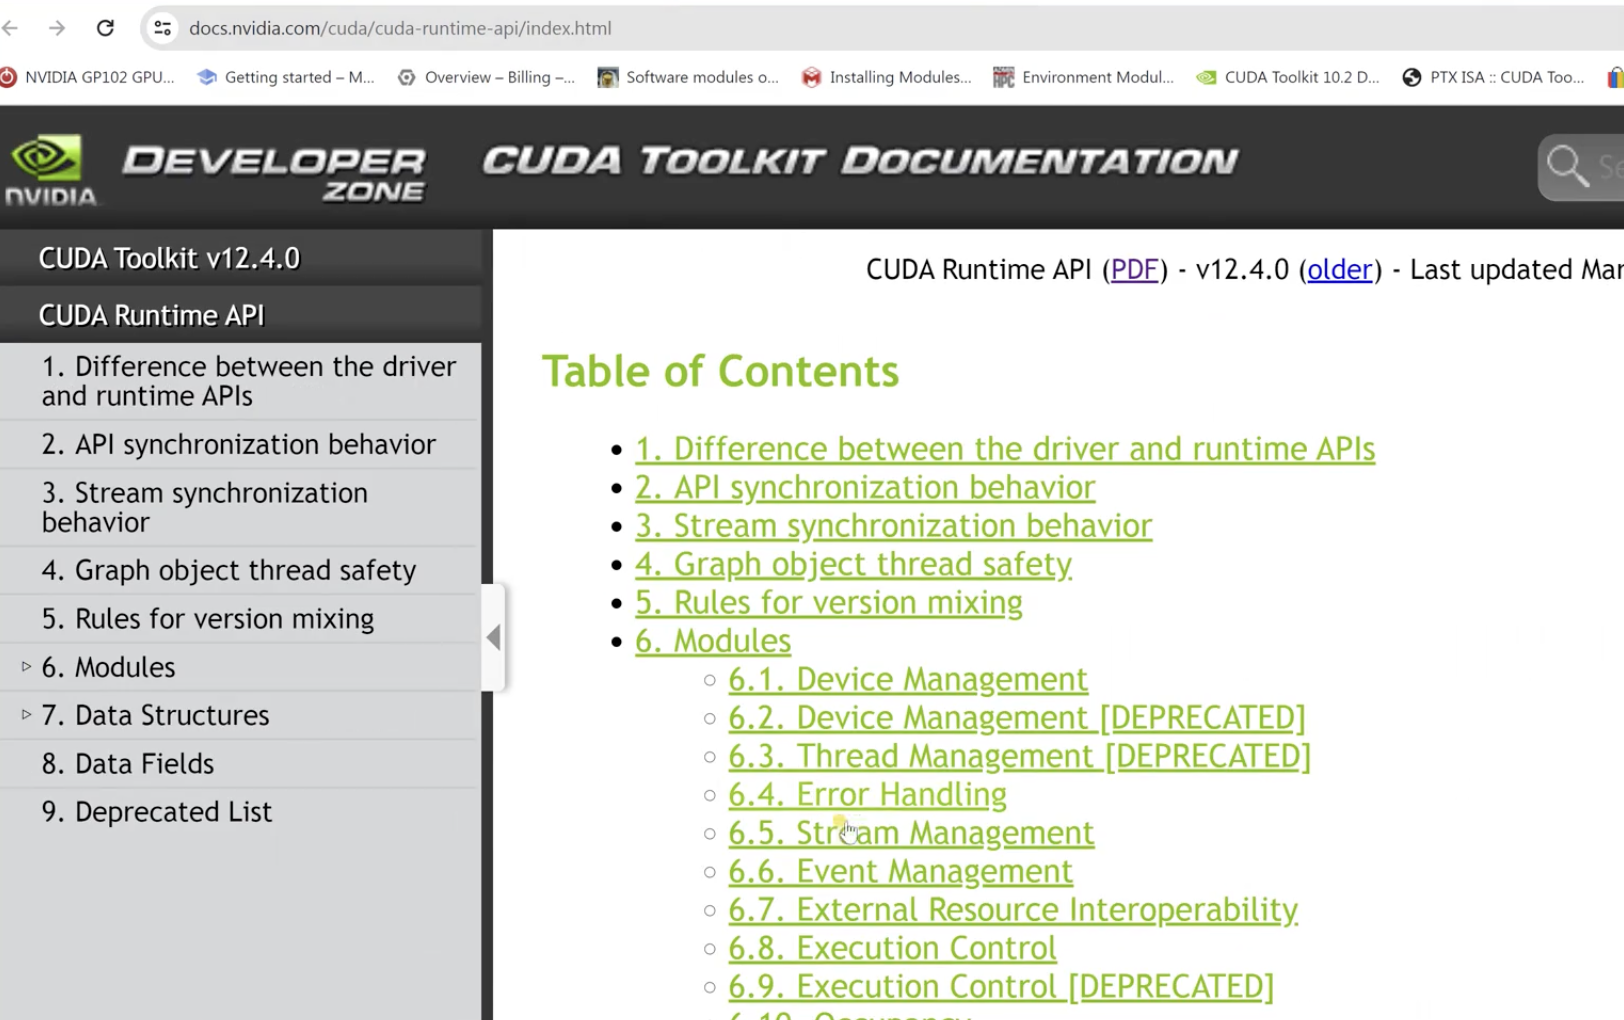
\includegraphics[width=0.75\linewidth]{resources/cuda-081.png}
    \caption{}
    \label{fig:placeholder}
\end{figure}


API函数最常见的例子之一是 \texttt{cudaGetDeviceProperties}函数。该函数旨在查询支持CUDA的GPU（或一般来说NVIDIA 
GPU）的属性和能力。这个函数为开发者提供了重要的信息，例如GPU名称、总全局内存、每个块的最大线程数、
计算能力以及其他指标。这些丰富的信息和指标使开发者能够优化他们的CUDA应用程序。
现在让我们将这个函数应用到我们的GPU上来查询它的属性。

\subsection{项目创建与代码实现}

为了开始我们今天的项目，我们需要进入创建CUDA文件的CUDA课程文件夹，然后从这里创建一个新文件。如我们所见，我选择
了 \texttt{section\_4\_01\_runtime\_api}，但在这里我要删除 \texttt{.txt} 并写上 \texttt{.cu}，
因为我们需要一个 \texttt{.cu}文件，而不是文本文件。然后你需要做的就是来到这里并打开这个文件，
使用任何编辑器（例如Visual StudioCode），然后点击 \texttt{Ctrl+S} 来保存我们的文件。

我要打开它，复制代码并粘贴到这个文件中。这里我想提醒你，这段代码的主要目的是查询GPU的一些属性，我们不需要进行任何计算
。这就是为什么我们在主函数之前没有任何GPU内核，就像我们在所有先前项目中习惯做的那样。

\subsection{代码解析}

\begin{lstlisting}
#include <stdio.h>

int main() {
    int nDevices;

    // 获取系统中可用GPU设备的数量
    cudaGetDeviceCount(&nDevices);

    // 遍历所有设备
    for (int i = 0; i < nDevices; i++) {
        cudaDeviceProp prop;
        
        // 获取设备ID为i的属性
        cudaGetDeviceProperties(&prop, i);

        printf("Device Number: %d\n", i);
        printf("  Device name: %s\n", prop.name);
        printf("  Memory Clock Rate (KHz): %d\n", prop.memoryClockRate);
        printf("  Memory Bus Width (bits): %d\n", prop.memoryBusWidth);
        
        // 峰值内存带宽计算示例（GB/s）
        // 注意：此处读取的是理论峰值而非实际运行值
        double peakBandwidth = 2.0 * prop.memoryClockRate * 
                              (prop.memoryBusWidth / 8) / 1.0e6;
        printf("  Peak Memory Bandwidth (GB/s): %f\n", peakBandwidth);
        
        printf("  Total Global Memory (Bytes): %zu\n", prop.totalGlobalMem);
        printf("  Compute Capability: %d.%d\n", prop.major, prop.minor);
        printf("  SM Count: %d\n", prop.multiProcessorCount);
        
        // 网格与块的限制
        printf("  Max threads per block: %d\n", prop.maxThreadsPerBlock);
        printf("  Max block dims: (%d, %d, %d)\n", 
               prop.maxThreadsDim[0], 
               prop.maxThreadsDim[1], 
               prop.maxThreadsDim[2]);
        printf("  Max grid dims: (%d, %d, %d)\n", 
               prop.maxGridSize[0], 
               prop.maxGridSize[1], 
               prop.maxGridSize[2]);
    }

    return 0;
}
\end{lstlisting}

\begin{figure}
    \centering
    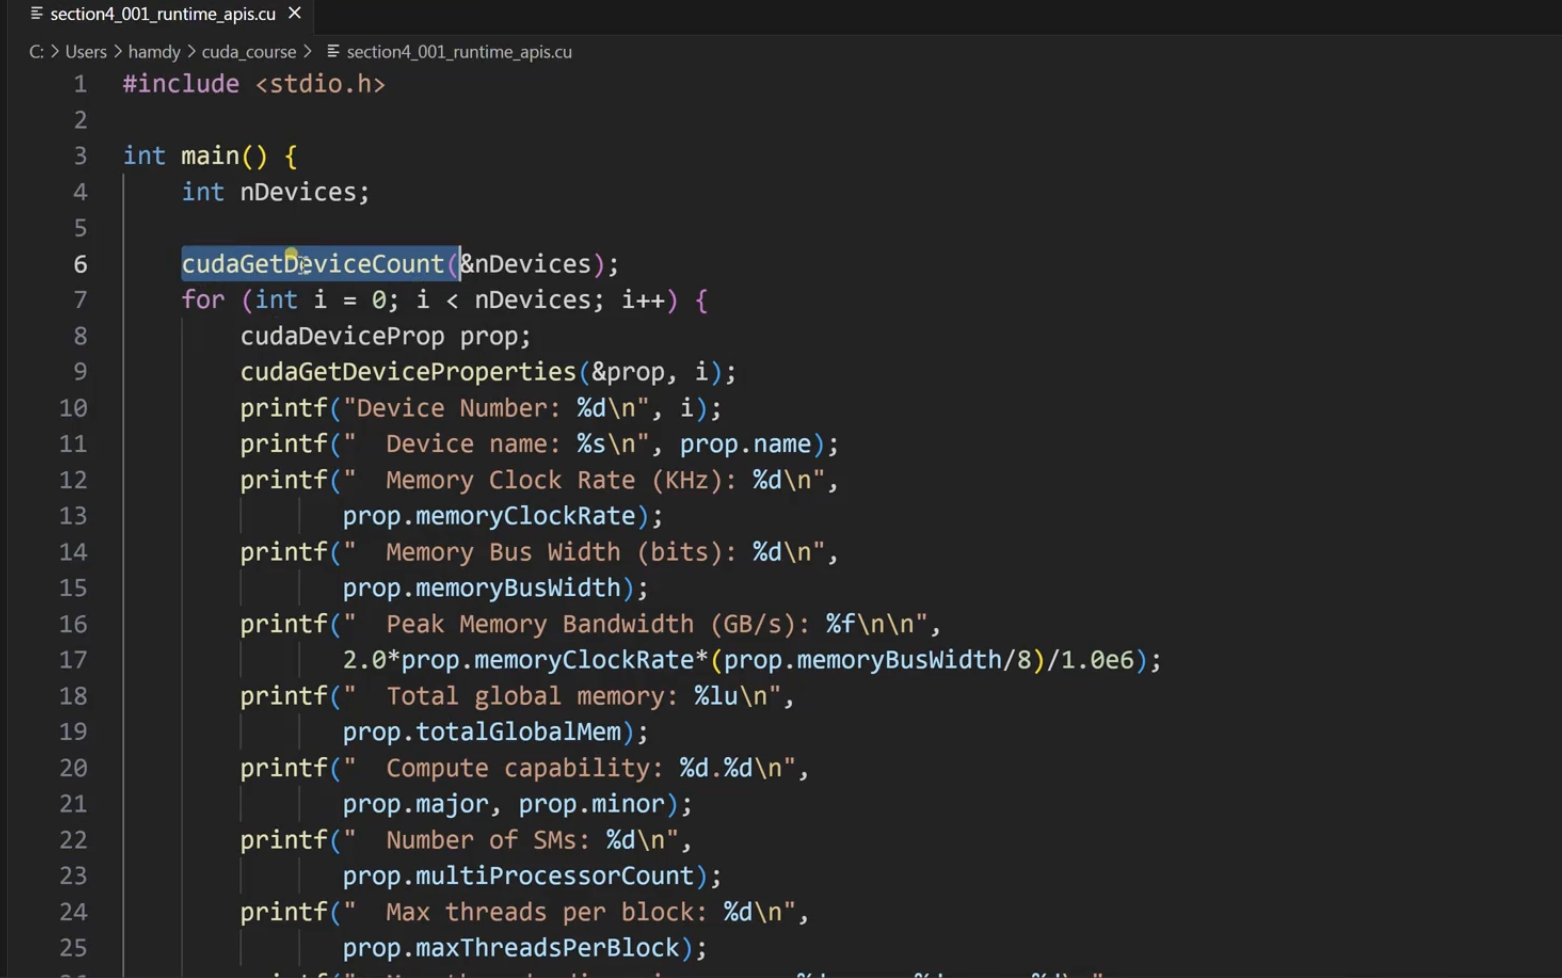
\includegraphics[width=0.75\linewidth]{resources/cuda-082.png}
    \caption{}
    \label{fig:placeholder}
\end{figure}

让我们从这里开始：

\begin{enumerate}
    \item 我们包含 \texttt{stdio.h} 库，以便能够使用 \texttt{printf}。
    \item 声明 \texttt{main} 函数，并为整型变量在内存中分配空间。
    \item 在第6行我们开始使用运行时API函数 \texttt{cudaGetDeviceCount}。函数的名称指的是它的任务：获取系统中设备的数量。如果系统中有3个NVIDIA GPU，那么数字3将存储在 \texttt{nDevices} 中。
    \item 使用 \texttt{for} 循环遍历计算机上所有的设备。我们从 \texttt{i=0} 开始，这指的是GPU编号0。
    \item 创建一个类型为 \texttt{cudaDeviceProp} 的结构体 \texttt{prop}。结构体意味着 \texttt{prop} 将包含不同的值，而不仅仅是一个值。
    \item 使用 \texttt{cudaGetDeviceProperties} 函数读取设备 \texttt{i} 的属性，并将结果存储在 \texttt{prop} 结构体中。
    \item 通过点操作符（\texttt{prop.name}, \texttt{prop.memoryClockRate} 等）访问并打印各项指标。
\end{enumerate}

\subsection{编译与运行验证}

使用NVCC编译器编译代码：

\begin{verbatim}
nvcc -o runtime_api section_4_01_runtime_api.cu
\end{verbatim}

运行可执行文件后，输出示例如下（以RTX 3090为例）：
\begin{itemize}
    \item \textbf{设备编号}: 0
    \item \textbf{设备名称}: GeForce RTX 3090
    \item \textbf{内存总线宽度}: 384 bits（与TechPowerUp数据库一致）
    \item \textbf{总全局内存}: 约24 GB（需将字节数除以 $1024^3$ 转换）
    \item \textbf{计算能力}: 8.6
    \item \textbf{SM数量}: 82
    \item \textbf{每块最大线程数}: 1024
    \item \textbf{最大块维度}: X=1024, Y=1024, Z=64
\end{itemize}

\begin{figure}
    \centering
    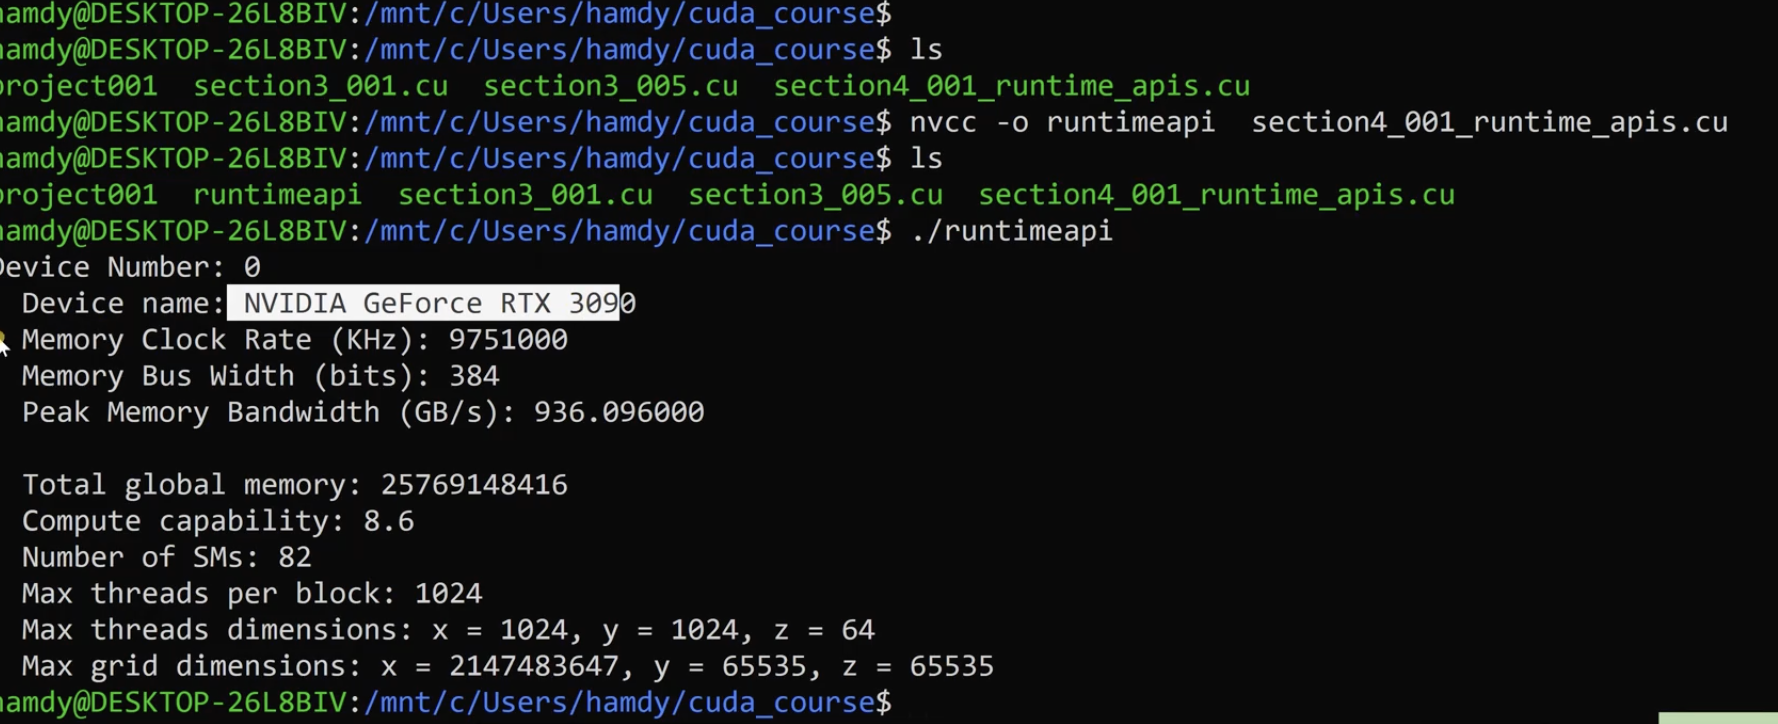
\includegraphics[width=0.75\linewidth]{resources/cuda-083.png}
    \caption{}
    \label{fig:placeholder}
\end{figure}


\textbf{思考题：} 已知每个Warp由32个线程组成，根据每块最大线程数1024，每个块的最大Warp数量是多少
？\[\text{Max Warps per Block} = \frac{1024}{32} = 32\]请注意区分“
块”（软件概念）和“SM”（硬件概念）。块在SM上执行，我们需要这个值来计算另一个性能指标——占用率（Occupancy）。

\subsection{关键要点总结}

\begin{enumerate}
    \item \textbf{参数传递机制}: 运行时API函数的运行方式与标准函数不同。它们不通过典型的返回机制返回结果，而是将输出分配给函数调用中提供的指针参数。例如 \texttt{cudaGetDeviceCount(\&nDevices)} 通过参数存储检测结果。
    
    \item \textbf{错误检查}: 运行时API函数返回它们的执行状态（\texttt{cudaError\_t}），该状态可以被捕获以供后续检查。如果成功则返回 \texttt{cudaSuccess}，否则返回错误代码，可用于分析故障原因。
    
    \item \textbf{效率优势}: 使用运行时API节省了大量时间。替代方案是在白皮书中查阅大量内容才能获取每一个参数值。虽然白皮书中有表格包含许多值，但并非全部，且API能动态反映当前设备的真实状态。
\end{enumerate}

今天就到这里，下个文章见。你需要知道如何使用运行时API，因为在接下来的文章中，我们在检查或分析性能时需要这些值。


\section{NVIDIA系统管理接口（nvidia-smi）详解}

本章将解释 NVIDIA 系统管理接口（System Management Interface），即 \texttt{nvidia-smi}。
\texttt{nvidia-smi} 是 NVIDIA 提供的一个命令行工具，为 NVIDIA GPU 提供监控和管理功能，可实时检查 NVIDIA GPU 状态。本章将探讨 \texttt{nvidia-smi} 的一些关键特性及使用示例。

\subsection{nvidia-smi 的三大关键领域}

\texttt{nvidia-smi} 可用于三个关键领域：性能监控、设置管理和设备信息查询。

\begin{figure}
    \centering
    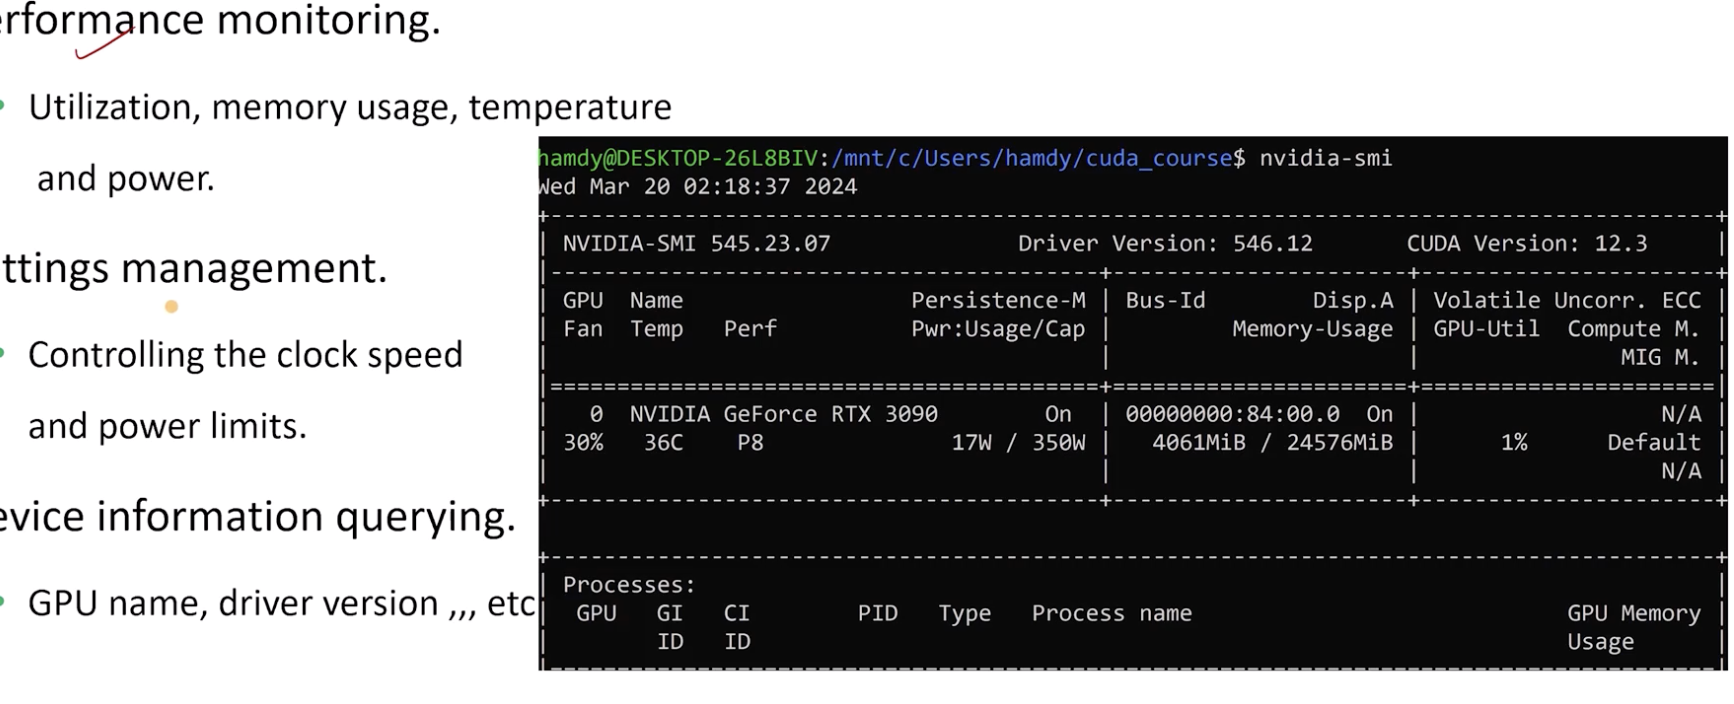
\includegraphics[width=0.75\linewidth]{resources/cuda-084.png}
    \caption{}
    \label{fig:placeholder}
\end{figure}

\begin{enumerate}
    \item \textbf{性能监控}: 可用于实时监控GPU性能，包括GPU资源利用率、内存使用情况、温度以及功耗。这些数据对于高效优化GPU资源至关重要。
    \item \textbf{设置管理}: 提供了调整或控制 GPU 内存和核心时钟速度的灵活性。不仅可以读取性能指标，还可以控制影响性能的参数。此外，可以为GPU功耗设定限制。
    \item \textbf{设备信息查询}: 提供关于GPU型号、驱动程序版本、CUDA版本以及当前时钟速度的全面详细信息。这确保开发者和管理员拥有必要的数据来做出关于软件兼容性和性能调优的明智决策。
\end{enumerate}

\subsection{基础命令与输出解读}

从最简单的命令开始：\texttt{nvidia-smi}。通过执行这个简单命令，我们可以获得性能指标的全面概览。
输出包含两个主要表格。

\subsection{第一个表格：性能概览}

第一行显示两个重要指标：
\begin{itemize}
    \item \textbf{驱动程序版本}: 例如 546.12。确认驱动版本有助于排查库兼容性问题。
    \item \textbf{CUDA版本}: 例如 12.3。可通过 \texttt{nvcc --version} 验证编译器版本是否匹配。
\end{itemize}

第二行是指标名称，第三行是对应值。该表格分为多列：
\begin{itemize}
    \item \textbf{GPU信息}: GPU名称（如 GeForce RTX 3090）、GPU ID（如 0）。
    \item \textbf{功耗与温度}: 当前功耗（如 31W）/ 最大功耗限制（如 350W）；当前温度（如 53°C）。
    \item \textbf{内存使用}: 已用显存 / 总显存（如 4000 MiB / 24 GiB）。
    \item \textbf{GPU 利用率}: 即使未运行自定义 CUDA 程序，若后台有录屏等应用调用 GPU 编码器，利用率也可能显示为 30\%-40\%。注意：\texttt{nvidia-smi} 的进程列表通常只显示 CUDA 计算进程，不一定显示视频编码/解码进程。
\end{itemize}

\begin{figure}
    \centering
    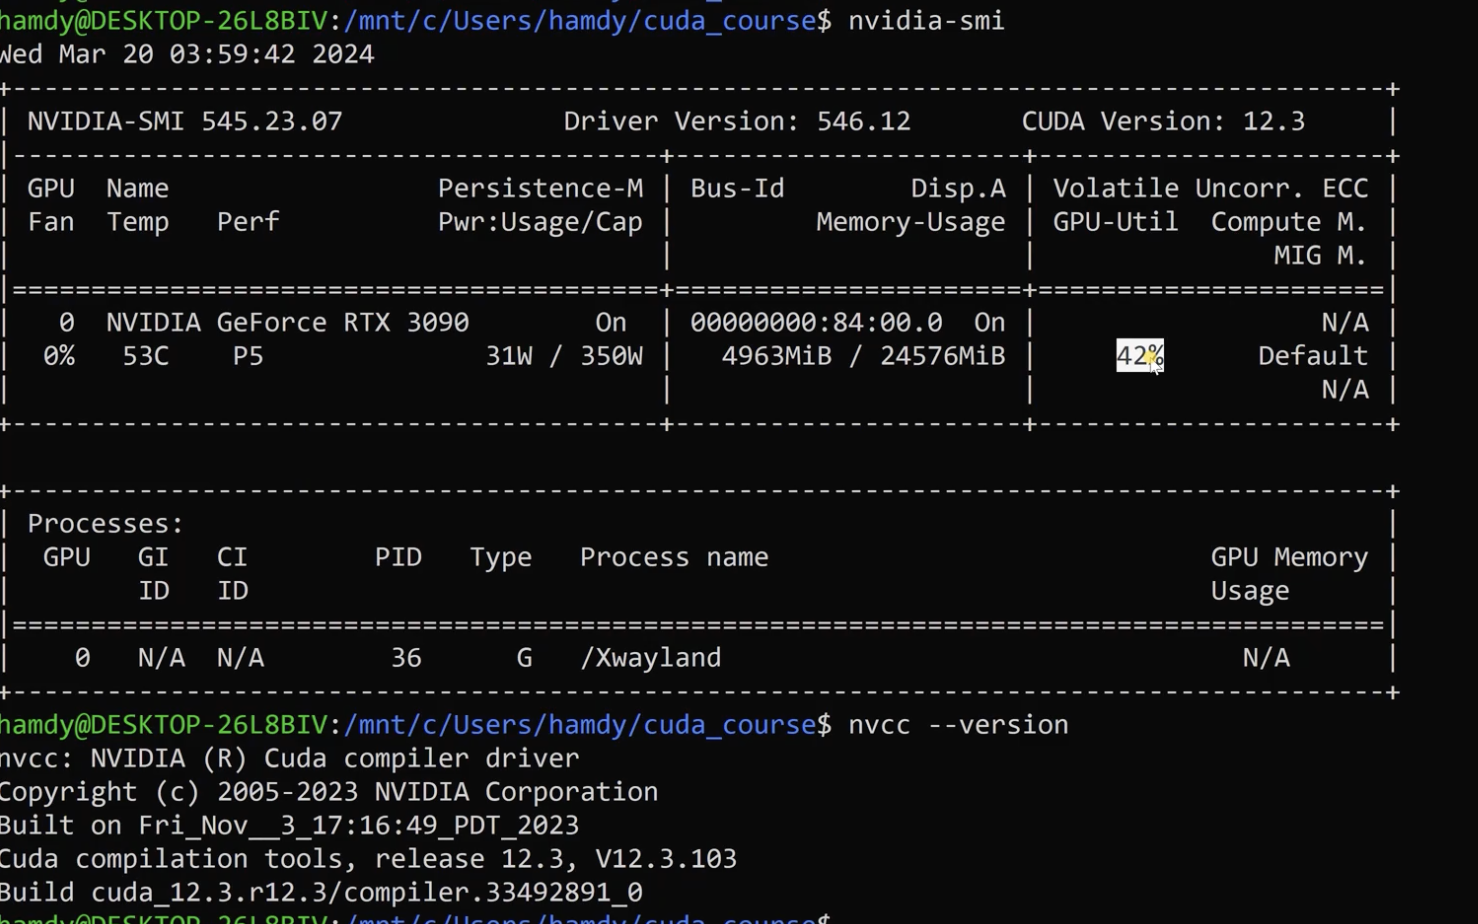
\includegraphics[width=0.75\linewidth]{resources/cuda-085.png}
    \caption{}
    \label{fig:placeholder}
\end{figure}

\subsection{第二个表格：进程列表}

此表格显示当前在GPU上运行的计算进程。例如运行矩阵乘法（Matrix Multiplication）应用时：
\begin{itemize}
    \item GPU利用率从空闲时的 $\sim$19\% 升至 100\%。
    \item 功耗从 $\sim$29W 升至 $\sim$318W（接近350W上限）。
    \item 温度从 36°C 升至 63°C。
    \item 显存占用显著增加（如增至 $\sim$8 GiB）。
\end{itemize}

\begin{figure}
    \centering
    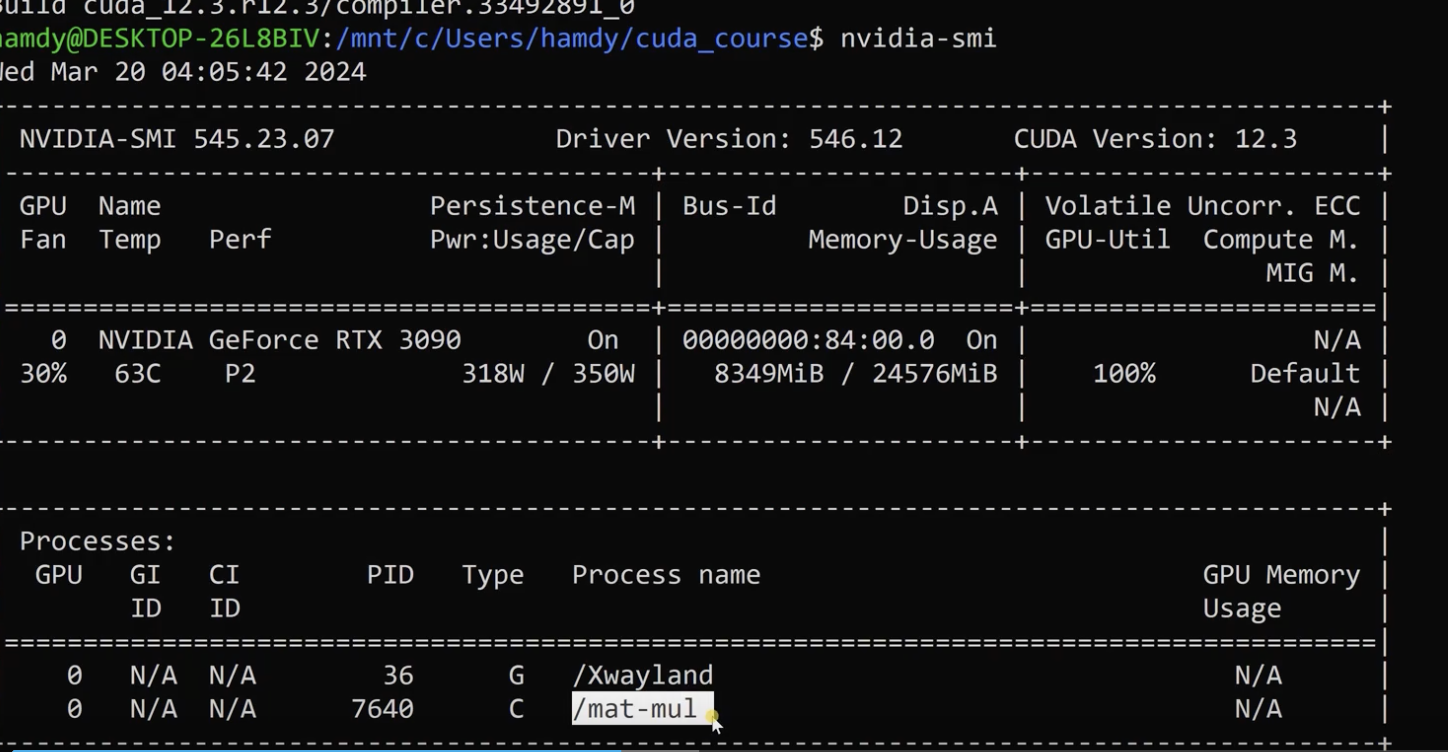
\includegraphics[width=0.75\linewidth]{resources/cuda-086.png}
    \caption{}
    \label{fig:placeholder}
\end{figure}

\subsection{持续监控与数据导出}

\subsection{循环查询模式}

使用 \texttt{-l} (loop) 参数实现持续监控：
\begin{lstlisting}
# 每5秒刷新一次
nvidia-smi -l 5

# 每2秒刷新一次
nvidia-smi -l 2
\end{lstlisting}
按 \texttt{Ctrl+C} 退出。通过对比刷新间隔内的数值变化，可以观察应用程序执行期间的实时性能波动。

\begin{figure}
    \centering
    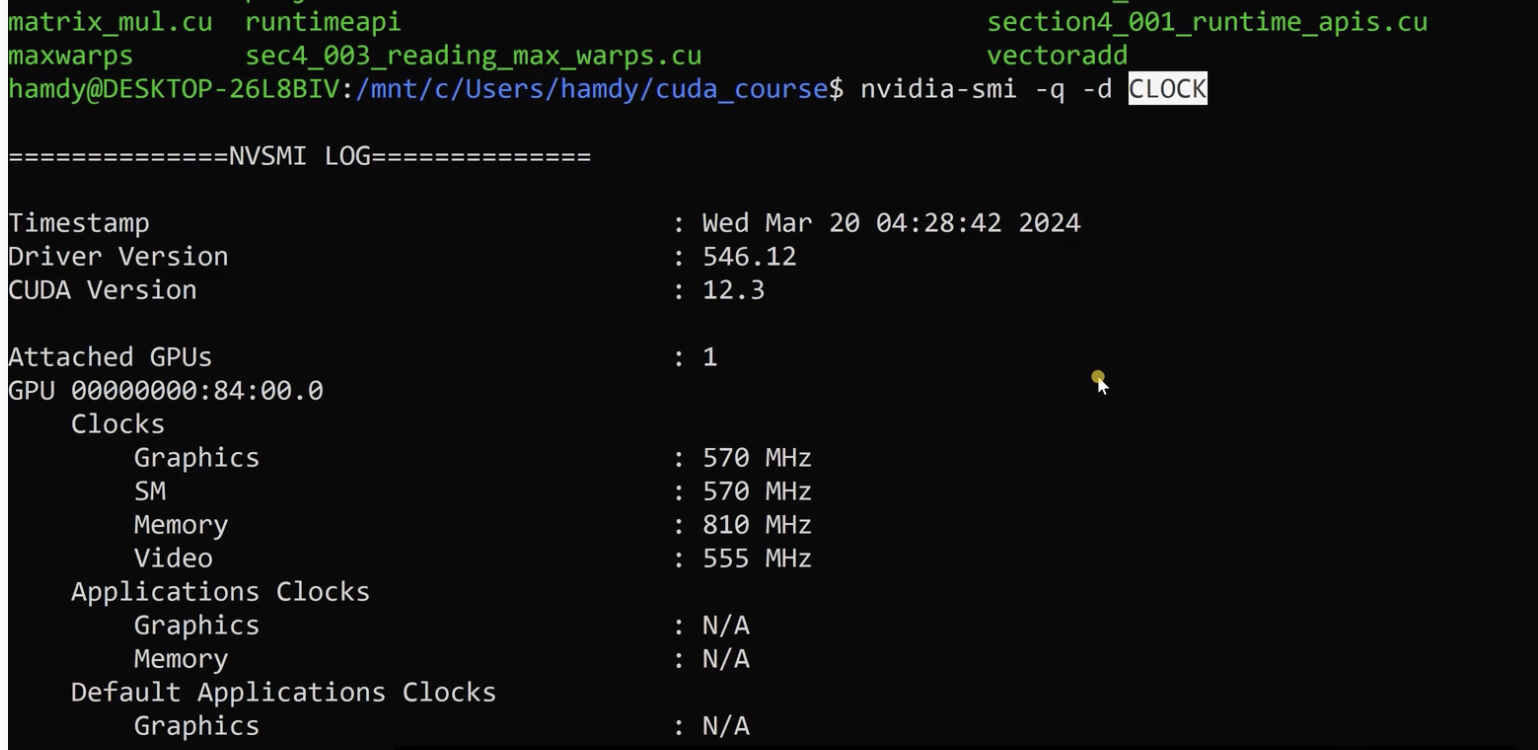
\includegraphics[width=0.75\linewidth]{resources/cuda-087.png}
    \caption{}
    \label{fig:placeholder}
\end{figure}

\subsection{定向查询与CSV导出}

使用 \texttt{--query-gpu} 和 \texttt{--format} 参数提取特定指标：
\begin{lstlisting}
# 查询指定指标并以CSV格式输出
nvidia-smi --query-gpu=name,driver_version,temperature.gpu \
           --format=csv

# 将结果保存到文件（Linux重定向）
nvidia-smi --query-gpu=name,driver_version,temperature.gpu \
           --format=csv > gpu_stats.csv
\end{lstlisting}
输出的CSV文件可直接用Excel打开进行分析。

\subsection{设置管理：功耗与时钟控制}

\subsection{功耗限制}

\begin{figure}
    \centering
    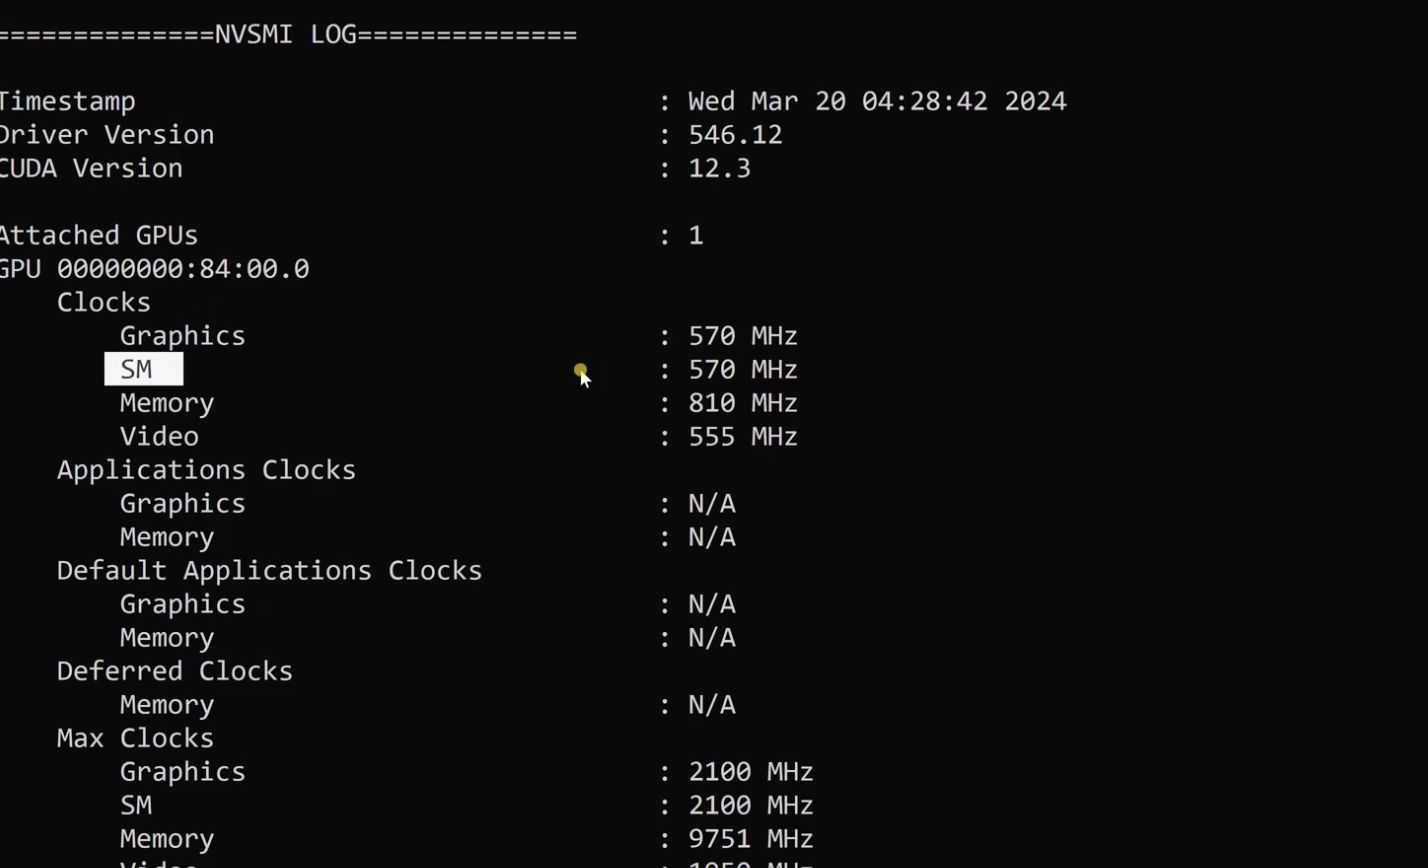
\includegraphics[width=0.75\linewidth]{resources/cuda-088.png}
    \caption{}
    \label{fig:placeholder}
\end{figure}

使用 \texttt{-pl} (power limit) 设置功耗上限：
\begin{lstlisting}
# 将GPU 0的功耗限制设为200W
sudo nvidia-smi -i 0 -pl 200
\end{lstlisting}
\textbf{注意}: 并非所有GPU都支持修改功耗限制，需提前确认硬件支持情况。

\subsection{持久模式（Persistence Mode）}

持久模式保持GPU驱动常驻内存，避免频繁加载/卸载开销。修改时钟等设置前可能需要先启用：
\begin{lstlisting}
# 启用持久模式
sudo nvidia-smi -i 0 -pm 1

# 禁用持久模式
sudo nvidia-smi -i 0 -pm 0
\end{lstlisting}

\subsection{时钟速度查询与控制}

\begin{figure}
    \centering
    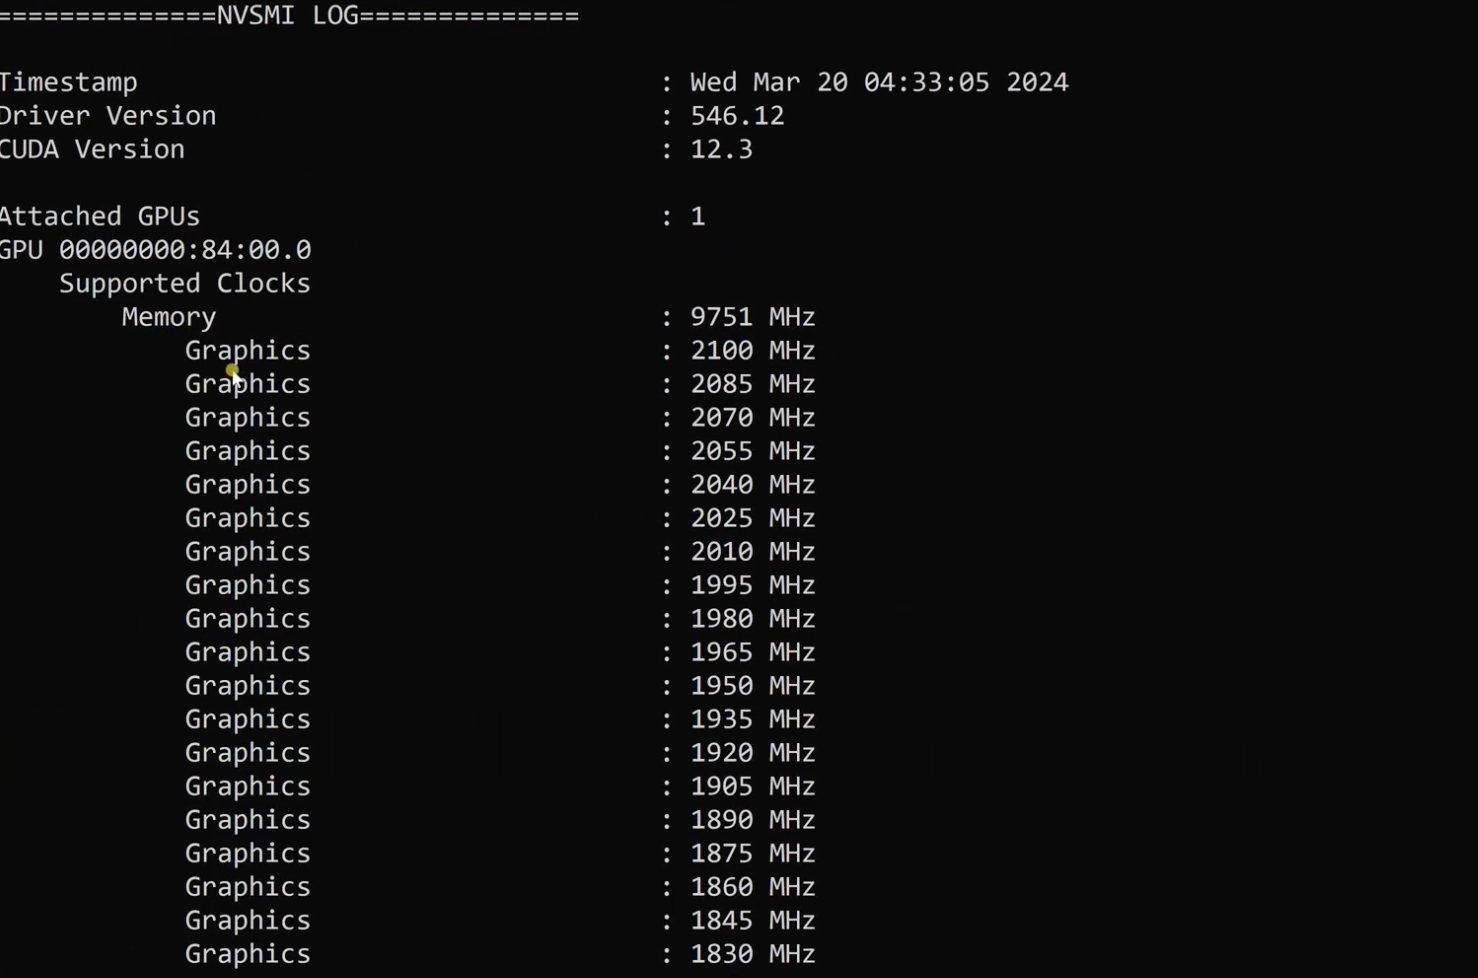
\includegraphics[width=0.75\linewidth]{resources/cuda-089.png}
    \caption{}
    \label{fig:placeholder}
\end{figure}


\subsection{查询时钟}

使用 \texttt{-q} (query) 查看时钟详情：
\begin{lstlisting}
nvidia-smi -q -d CLOCK
\end{lstlisting}
输出区分“当前时钟”与“最大时钟”。空闲时 GPU 会自动降频节能（如 SM 时钟从 2100 MHz 降至 570 MHz）；负载增加时自动升频（如升至 1695 MHz）。

\begin{lstlisting}
colin@colin-BATTLE-AX-B860M-P-WIFI:~$ nvidia-smi -q -d CLOCK

==============NVSMI LOG==============

Timestamp                                              : Sat Sep 26 11:19:58 2026
Driver Version                                         : 595.84
CUDA Version                                           : 13.2

Attached GPUs                                          : 1
GPU 00000000:02:00.0
    Clocks
        Graphics                                       : 180 MHz
        SM                                             : 180 MHz
        Memory                                         : 405 MHz
        Video                                          : 600 MHz
    Applications Clocks
        Graphics                                       : Requested functionality has been deprecated
        Memory                                         : Requested functionality has been deprecated
    Default Applications Clocks
        Graphics                                       : Requested functionality has been deprecated
        Memory                                         : Requested functionality has been deprecated
    Deferred Clocks
        Memory                                         : N/A
    Max Clocks
        Graphics                                       : 3090 MHz
        SM                                             : 3090 MHz
        Memory                                         : 14001 MHz
        Video                                          : 3090 MHz
    Max Customer Boost Clocks
        Graphics                                       : N/A
    SM Clock Samples
        Duration                                       : N/A
        Number of Samples                              : N/A
        Max                                            : N/A
        Min                                            : N/A
        Avg                                            : N/A
    Memory Clock Samples
        Duration                                       : N/A
        Number of Samples                              : N/A
        Max                                            : N/A
        Min                                            : N/A
        Avg                                            : N/A
    Clock Policy
        Auto Boost                                     : N/A
        Auto Boost Default                             : N/A
\end{lstlisting}

\subsection{查询支持的时钟频率}

设置固定时钟前，必须查询GPU支持的离散频率点：
\begin{lstlisting}
nvidia-smi -q -d SUPPORTED_CLOCKS
\end{lstlisting}
只能选择列表中存在的值（如内存 9501 MHz、5001 MHz；SM 12085 MHz、12070 MHz 等），不支持任意值。

\subsection{设置应用时钟}

使用 \texttt{-ac} (application clocks) 锁定SM和内存时钟：
\begin{lstlisting}
# 格式: -ac <mem_clock>,<sm_clock>
sudo nvidia-smi -i 0 -ac 9501,12085
\end{lstlisting}

\subsection{重置为默认值}

使用 \texttt{-r} 或 \texttt{-rac} / \texttt{-pmc} 重置设置：
\begin{lstlisting}
# 重置应用时钟为默认
sudo nvidia-smi -i 0 -rac

# 重置功耗限制为默认
sudo nvidia-smi -i 0 -pmc
\end{lstlisting}

\subsection{帮助与总结}

\begin{figure}
    \centering
    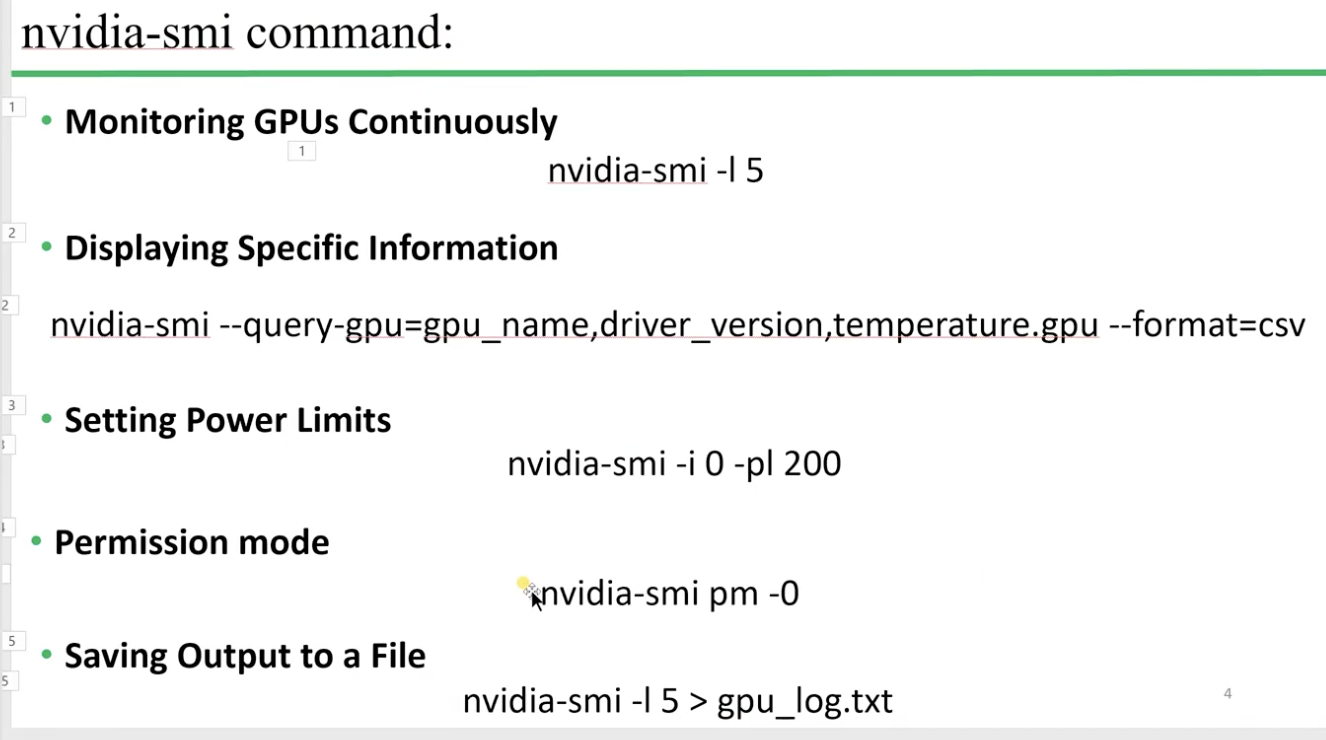
\includegraphics[width=0.75\linewidth]{resources/cuda-090.png}
    \caption{}
    \label{fig:placeholder}
\end{figure}

查看所有可用选项：
\begin{lstlisting}
nvidia-smi -h
\end{lstlisting}

\begin{lstlisting}
colin@colin-BATTLE-AX-B860M-P-WIFI:~$ nvidia-smi -h
NVIDIA System Management Interface -- v595.84

NVSMI provides monitoring information for Tesla and select Quadro devices.
The data is presented in either a plain text or an XML format, via stdout or a file.
NVSMI also provides several management operations for changing the device state.

Note that the functionality of NVSMI is exposed through the NVML C-based
library. See the NVIDIA developer website for more information about NVML.
Python wrappers to NVML are also available.  The output of NVSMI is
not guaranteed to be backwards compatible; NVML and the bindings are backwards
compatible.

http://developer.nvidia.com/nvidia-management-library-nvml/
http://pypi.python.org/pypi/nvidia-ml-py/
Supported products:
- Full Support
    - All Tesla products, starting with the Kepler architecture
    - All Quadro products, starting with the Kepler architecture
    - All GRID products, starting with the Kepler architecture
    - GeForce Titan products, starting with the Kepler architecture
- Limited Support
    - All Geforce products, starting with the Kepler architecture
nvidia-smi [OPTION1 [ARG1]] [OPTION2 [ARG2]] ...

    -h,   --help                Print usage information and exit.

          --version             Print version information and exit.

  LIST OPTIONS:

    -L,   --list-gpus           Display a list of GPUs connected to the system.

    -B,   --list-excluded-gpus  Display a list of excluded GPUs in the system.

  SUMMARY OPTIONS:

    <no arguments>              Show a summary of GPUs connected to the system.

    -col, --columns             Show a summary of GPUs connected to the system in multi-column format.

    [plus any of]

    -i,   --id=                 Target a specific GPU.
    -f,   --filename=           Log to a specified file, rather than to stdout.
    -l,   --loop=               Probe until Ctrl+C at specified second interval.

  QUERY OPTIONS:

    -q,   --query               Display GPU or Unit info.

    [plus any of]

    -u,   --unit                Show unit, rather than GPU, attributes.
    -i,   --id=                 Target a specific GPU or Unit.
    -f,   --filename=           Log to a specified file, rather than to stdout.
    -x,   --xml-format          Produce XML output.
          --dtd                 When showing xml output, embed DTD.
    -d,   --display=            Display only selected information: MEMORY,
                                    UTILIZATION, ECC, TEMPERATURE, POWER, CLOCK,
                                    COMPUTE, PIDS, PERFORMANCE, SUPPORTED_CLOCKS,
                                    PAGE_RETIREMENT, ACCOUNTING, ENCODER_STATS,
                                    SUPPORTED_GPU_TARGET_TEMP, VOLTAGE, FBC_STATS
                                    ROW_REMAPPER, GSP_FIRMWARE_VERSION
                                    POWER_SMOOTHING, POWER_PROFILES
                                Flags can be combined with comma e.g. ECC,POWER.
                                Sampling data with max/min/avg is also returned
                                for POWER, UTILIZATION and CLOCK display types.
                                Doesn't work with -u or -x flags.
    -l,   --loop=               Probe until Ctrl+C at specified second interval.

    -lms, --loop-ms=            Probe until Ctrl+C at specified millisecond interval.

  SELECTIVE QUERY OPTIONS:

    Allows the caller to pass an explicit list of properties to query.

    [one of]

    --query-gpu                 Information about GPU.
                                Call --help-query-gpu for more info.
    --query-supported-clocks    List of supported clocks.
                                Call --help-query-supported-clocks for more info.
    --query-compute-apps        List of currently active compute processes.
                                Call --help-query-compute-apps for more info.
    --query-accounted-apps      List of accounted compute processes.
                                Call --help-query-accounted-apps for more info.
                                This query is not supported on vGPU host.
    --query-retired-pages       List of device memory pages that have been retired.
                                Call --help-query-retired-pages for more info.
    --query-remapped-rows       Information about remapped rows.
                                Call --help-query-remapped-rows for more info.

    [mandatory]

    --format=                   Comma separated list of format options:
                                  csv - comma separated values (MANDATORY)
                                  noheader - skip the first line with column headers
                                  nounits - don't print units for numerical
                                             values

    [plus any of]

    -i,   --id=                 Target a specific GPU or Unit.
    -f,   --filename=           Log to a specified file, rather than to stdout.
    -l,   --loop=               Probe until Ctrl+C at specified second interval.
    -lms, --loop-ms=            Probe until Ctrl+C at specified millisecond interval.

  DEVICE MODIFICATION OPTIONS:

    [any one of]

    -pm,  --persistence-mode=   Set persistence mode: 0/DISABLED, 1/ENABLED
    -e,   --ecc-config=         Toggle ECC support: 0/DISABLED, 1/ENABLED
    -p,   --reset-ecc-errors=   Reset ECC error counts: 0/VOLATILE, 1/AGGREGATE
    -c,   --compute-mode=       Set MODE for compute applications:
                                0/DEFAULT, 1/EXCLUSIVE_THREAD (DEPRECATED),
                                2/PROHIBITED, 3/EXCLUSIVE_PROCESS
          --gom=                Set GPU Operation Mode:
                                    0/ALL_ON, 1/COMPUTE, 2/LOW_DP
    -r    --gpu-reset           Trigger reset of the GPU.
                                Can be used to reset the GPU HW state in situations
                                that would otherwise require a machine reboot.
                                Typically useful if a double bit ECC error has
                                occurred.
                                Reset operations are not guaranteed to work in
                                all cases and should be used with caution.
                                Reset triggered without extra arguments, will be a.
                                default Function Level Reset (FLR). To issue a
                                Bus Reset, use -r bus.
    -vm   --virt-mode=          Switch GPU Virtualization Mode:
                                Sets GPU virtualization mode to 3/VGPU or 4/VSGA
                                Virtualization mode of a GPU can only be set when
                                it is running on a hypervisor.
    -lgc  --lock-gpu-clocks=    Specifies <minGpuClock,maxGpuClock> clocks as a
                                    pair (e.g. 1500,1500) that defines the range
                                    of desired locked GPU clock speed in MHz.
                                    Setting this will supersede application clocks
                                    and take effect regardless if an app is running.
                                    Input can also be a singular desired clock value
                                    (e.g. <GpuClockValue>). Optionally, --mode can be
                                    specified to indicate a special mode.
    -m    --mode=               Specifies the mode for --lock-gpu-clocks.
                                    Valid modes: 0, 1
    -rgc  --reset-gpu-clocks
                                Resets the GPU clocks to the default values.
    -lmc  --lock-memory-clocks=  Specifies <minMemClock,maxMemClock> clocks as a
                                    pair (e.g. 5100,5100) that defines the range
                                    of desired locked Memory clock speed in MHz.
                                    Input can also be a singular desired clock value
                                    (e.g. <MemClockValue>).
    -rmc  --reset-memory-clocks
                                Resets the Memory clocks to the default values.
    -lmcd --lock-memory-clocks-deferred=
                                    Specifies memClock clock to lock. This limit is
                                    applied the next time GPU is initialized.
                                    This is guaranteed by unloading and reloading the kernel module.
                                    Requires root.
    -rmcd --reset-memory-clocks-deferred
                                Resets the deferred Memory clocks applied.
    -ac   --applications-clocks= Specifies <memory,graphics> clocks as a
                                    pair (e.g. 2000,800) that defines GPU's
                                    speed in MHz while running applications on a GPU.
    -rac  --reset-applications-clocks
                                Resets the applications clocks to the default values.
    -pl   --power-limit=        Specifies maximum power management limit in watts.
                                Takes an optional argument --scope.
    -sc   --scope=              Specifies the device type for --scope: 0/GPU, 1/TOTAL_MODULE (Grace Hopper Only)
    -cc   --cuda-clocks=        Overrides or restores default CUDA clocks.
                                In override mode, GPU clocks higher frequencies when running CUDA applications.
                                Only on supported devices starting from the Volta series.
                                Requires administrator privileges.
                                0/RESTORE_DEFAULT, 1/OVERRIDE
    -am   --accounting-mode=    Enable or disable Accounting Mode: 0/DISABLED, 1/ENABLED
    -caa  --clear-accounted-apps
                                Clears all the accounted PIDs in the buffer.
          --auto-boost-default= Set the default auto boost policy to 0/DISABLED
                                or 1/ENABLED, enforcing the change only after the
                                last boost client has exited.
          --auto-boost-permission=
                                Allow non-admin/root control over auto boost mode:
                                0/UNRESTRICTED, 1/RESTRICTED
    -mig  --multi-instance-gpu= Enable or disable Multi Instance GPU: 0/DISABLED, 1/ENABLED
                                Requires root.
    -gtt  --gpu-target-temp=    Set GPU Target Temperature for a GPU in degree celsius.
                                Requires administrator privileges
    -den, --dram-encryption=    Toggle DRAM Encryption support: 0/DISABLED, 1/ENABLED
                                Requires root.
           --set-hostname=      Set the hostname associated with the GPU.
                                Requires root.
           --get-hostname       Get the hostname associated with the GPU.

   [plus optional]

    -i,   --id=                 Target a specific GPU.
    -eow, --error-on-warning    Return a non-zero error for warnings.

  UNIT MODIFICATION OPTIONS:

    -t,   --toggle-led=         Set Unit LED state: 0/GREEN, 1/AMBER

   [plus optional]

    -i,   --id=                 Target a specific Unit.

  SHOW DTD OPTIONS:

          --dtd                 Print device DTD and exit.

     [plus optional]

    -f,   --filename=           Log to a specified file, rather than to stdout.
    -u,   --unit                Show unit, rather than device, DTD.

    --debug=                    Log encrypted debug information to a specified file.

 Device Monitoring:
    dmon                        Displays device stats in scrolling format.
                                "nvidia-smi dmon -h" for more information.

    daemon                      Runs in background and monitor devices as a daemon process.
                                This is an experimental feature. Not supported on Windows baremetal
                                "nvidia-smi daemon -h" for more information.

    replay                      Used to replay/extract the persistent stats generated by daemon.
                                This is an experimental feature.
                                "nvidia-smi replay -h" for more information.

 Process Monitoring:
    pmon                        Displays process stats in scrolling format.
                                "nvidia-smi pmon -h" for more information.

 TOPOLOGY:
    topo                        Displays device/system topology. "nvidia-smi topo -h" for more information.

 DRAIN STATES:
    drain                       Displays/modifies GPU drain states for power idling. "nvidia-smi drain -h" for more information.

 NVLINK:
    nvlink                      Displays device nvlink information. "nvidia-smi nvlink -h" for more information.

 C2C:
    c2c                         Displays device C2C information. "nvidia-smi c2c -h" for more information.

 CLOCKS:
    clocks                      Control and query clock information. "nvidia-smi clocks -h" for more information.

 ENCODER SESSIONS:
    encodersessions             Displays device encoder sessions information. "nvidia-smi encodersessions -h" for more information.

 FBC SESSIONS:
    fbcsessions                 Displays device FBC sessions information. "nvidia-smi fbcsessions -h" for more information.

 GRID vGPU:
    vgpu                        Displays vGPU information. "nvidia-smi vgpu -h" for more information.

 MIG:
    mig                         Provides controls for MIG management. "nvidia-smi mig -h" for more information.

 COMPUTE POLICY:
    compute-policy              Control and query compute policies. "nvidia-smi compute-policy -h" for more information.

 BOOST SLIDER:
    boost-slider                Control and query boost sliders. "nvidia-smi boost-slider -h" for more information.

 POWER HINT:
    power-hint                  Estimates GPU power usage. "nvidia-smi power-hint -h" for more information.

 BASE CLOCKS:
    base-clocks                 Query GPU base clocks. "nvidia-smi base-clocks -h" for more information.

 CONFIDENTIAL COMPUTE:
    conf-compute                Control and query confidential compute. "nvidia-smi conf-compute -h" for more information.

 GPU PERFORMANCE MONITORING:
    gpm                         Control and query GPU performance monitoring unit. "nvidia-smi gpm -h" for more information.

 PCI:
    pci                         Display device PCI information. "nvidia-smi pci -h" for more information.

 Power Smoothing:
    power-smoothing             Control and query power smoothing information. "nvidia-smi power-smoothing -h" for more information.

 Power Profiles:
    power-profiles              Control and query workload power profiles information. "nvidia-smi power-profiles -h" for more information.

 RUSD:
    rusd                         Set RUSD (read only shared data buffer) settings. "nvidia-smi rusd -h" for more information.

 PRM:
    prm                         Query GPU PRM registers. "nvidia-smi prm -h" for more information.

 SOC:
    soc                          Query system on chip metrics. "nvidia-smi soc -h" for more information.

Please see the nvidia-smi(1) manual page for more detailed information.
\end{lstlisting}

\texttt{nvidia-smi} 是一个非常重要的命令。在后续章节中，将使用 \texttt{nvidia-smi} 来检查各种性能指标，验证优化效果，并诊断 GPU 运行状态。


\section{GPU占用率与延迟隐藏技术详解}

\subsection{引言：占用率的概念区分}

本章将深入探讨占用率（Occupancy）和利用率这两个概念，即比较不同架构时所需的关键参数。本章开头有必要重温课程中一个重要章节的内容——讨论了一系列关键参数，如内存带宽和指令吞吐量。在本章中，将引入占用率作为另一个评估性能的关键术语。

这个术语的真正问题在于，大多数涉及该主题的教程倾向于只解释理论占用率，而不是实际达到的占用率。GPU 的占用率是衡量 GPU 中资源利用率的一个指标。在 GPU 性能领域，占用率被分为两种不同的类型：理论占用率代表理想化场景，达到的占用率表示 GPU 资源的实际使用情况。

理论占用率的计算方法是将核函数中使用的 Warp 数除以每个 SM（流式多处理器）所能容纳的最大 Warp 数。这里涉及两个关键值：分子根据应用程序中使用的 Warp 数而变化；分母对应 GPU 的 Warp 数限制，这个限制可以从 GPU 白皮书中获取，或者使用前文介绍的运行时 API 获取。

\subsection{获取硬件限制：运行时API示例}

\begin{figure}
    \centering
    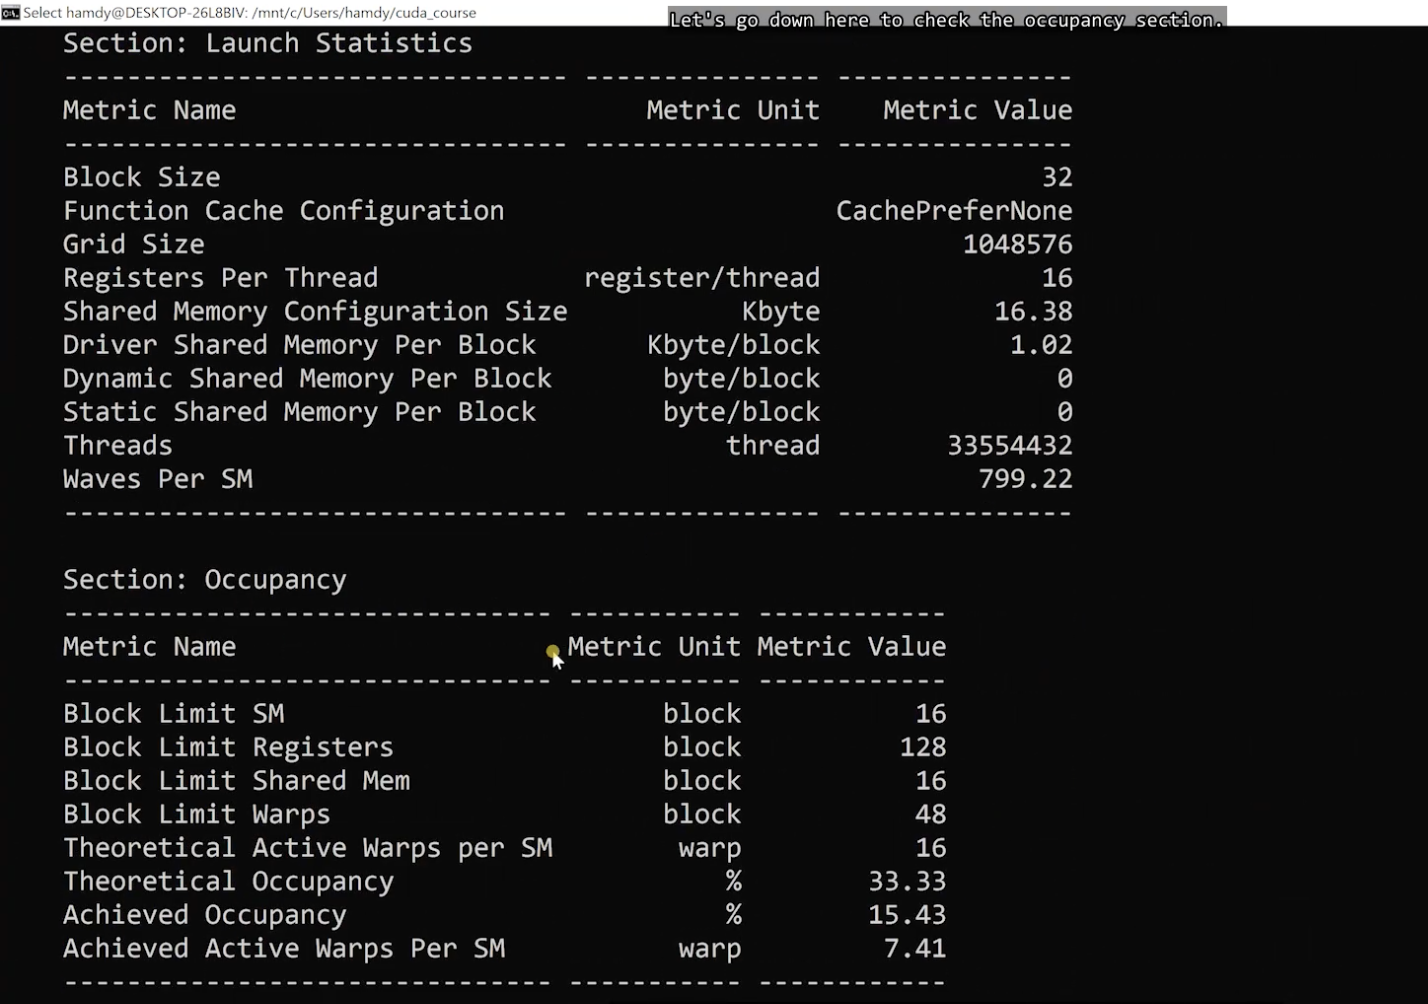
\includegraphics[width=0.75\linewidth]{resources/cuda-091.png}
    \caption{}
    \label{fig:placeholder}
\end{figure}

运行一个简单的代码，它包含运行时 API 函数，用于获取 GPU 每个 SM 的最大 Warp 数。首先使用 \texttt{nvidia-smi} 命令来识别 GPU 的名称，以获取方程的分母。如输出所示，GPU 是 GeForce 系列的一员，具体型号是 RTX 3090。

既然已经确定了正在处理的是哪个 GPU，现在把注意力转向代码，类似于前文的方法。从 \texttt{cudaGetDeviceCount} 函数开始，它提供系统中可用的支持 CUDA 的 GPU 总数。如果有两块 NVIDIA GPU 和一块 AMD GPU，AMD GPU 将不会包含在此变量中，即该变量只会包含 2 而不是 3。

然后使用 \texttt{cudaDeviceProp} 结构体来创建对象，用于存储所选 GPU 的所有属性。如果只有一个 GPU，使用索引 0 即可，无需使用 for 循环遍历所有 GPU。这里的 \texttt{cudaGetDeviceProperties} 函数读取 GPU 的所有属性，从 GPU ID=0 读取的属性将被存储在这个对象中。

这里打印的是每个 SM 的最大 Warp 数。如果想打印此对象中的任何度量指标，需要使用点运算符。例如 \texttt{prop.maxThreadsPerMultiProcessor} 获取每个 SM 的最大线程数，再除以 32 即可得到最大 Warp 数，因为每个 Warp 包含 32 个线程。

还有另一种读取这些度量指标的方法，涉及使用 \texttt{cudaDeviceGetAttribute} 函数。从其名称可知，此函数可用于从任何设备读取单个属性。例如在这种情况下，需要读取每个 SM 的最大 Warp 数，只需写入属性的名称，属性名称可以在该函数的文档中查到。

在文档中搜索该函数，它接受三个参数：第一个是值（存储结果），第二个是度量指标或属性的名称，最后一个是设备 ID。如果计算机中有多个 GPU，需要确定是从 GPU ID=0 还是 ID=1 或 ID=2 读取。如所示，有几十个可以读取的属性，例如每个块的最大寄存器数、多处理器数量、ECC 错误纠正、内存时钟频率等。前文已通过 \texttt{nvidia-smi} 命令检查过内存时钟频率，这里是读取它的另一种方法。

这里需要的度量指标是 \texttt{cudaDevAttrMaxThreadsPerMultiProcessor}。这个函数需要两个输入：设备 ID 和属性名称，然后属性值将被存储在定义为整数的变量中。同时可以将该值除以 32 以获得每个 SM 的最大 Warp 数。

进入 CUDA 课程文件夹，列出所有可用文件。复制文件名，然后使用 nvcc 编译器，将可执行文件命名为 \texttt{read\_metrics}，放上 \texttt{.cu} 文件，点击回车。执行后，如所示，RTX 3090 GPU 中每个 SM 的最大 Warp 数是 48（1536/32）。使用第二个函数结果也一样，两种方法都可以使用。

\subsection{理论占用率计算示例}

现在已知每个 SM 的最大 Warp 数是 48。看一些例子来理解理论占用率。

在第一个场景中，考虑一个设计为使用每个 SM 48 个 Warp 的 CUDA 应用程序。计算比率得出理论占用率为 100\%，因为应用程序中使用的 48 个 Warp 与每个 SM 的 Warp 上限 48 相匹配。

在第二个场景中，如果应用程序配置为使用每个 SM 12 个 Warp，那么 $12/48$ 的比率表明理论占用率降低到了 25\%。然而在后续两个章节中，将探讨更复杂的场景。因为占用率与另一个称为"每个 SM 分配的活动块"的术语有关，该术语将在后续章节中探讨，这里只是简化的例子。

\subsection{向量加法案例研究}

\begin{figure}
    \centering
    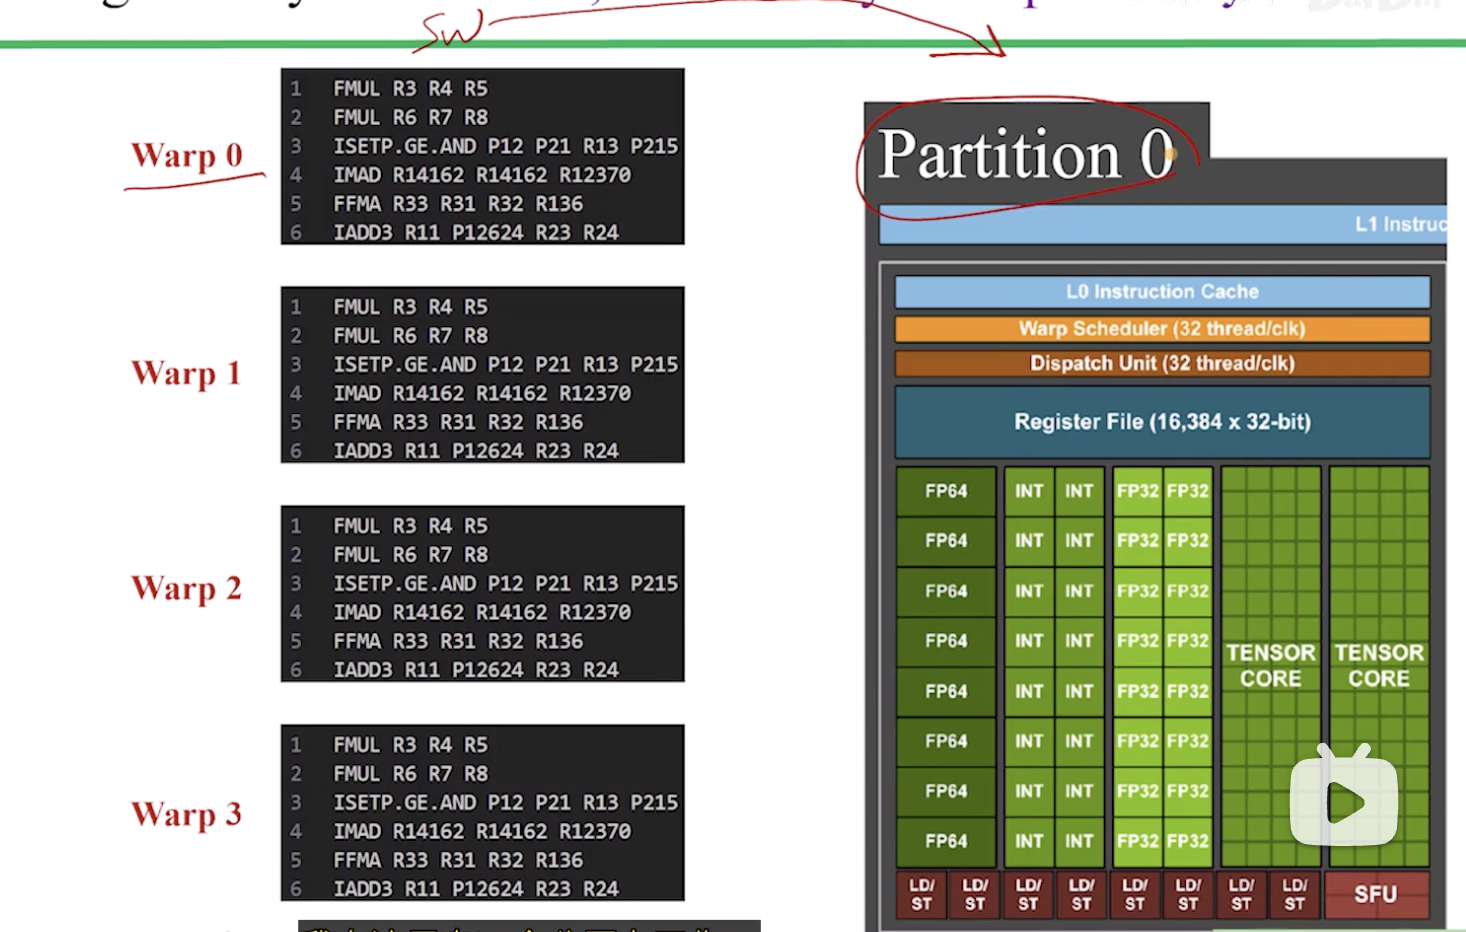
\includegraphics[width=0.75\linewidth]{resources/cuda-092.png}
    \caption{}
    \label{fig:placeholder}
\end{figure}

深入评估与向量加法应用相关的理论占用率。本章的主要目的是专注于占用率这个术语，因此不会解释 Nsight Compute 工具中的不同选项，仅使用最简单的命令。

列出文件夹中所有的 CUDA 文件，复制向量加法文件并进行编译：\texttt{nvcc -o vector\_add vector\_add.cu}。如所示，它正确执行了，执行时间大约为 6.5 毫秒。

需要分析这个应用，可以使用 \texttt{ncu} 命令（即 Nsight Compute）。如所示，分析过程已启动。从头开始看：核函数名称是 \texttt{vectorAdd}，这些是核函数的输入参数和维度。可以从 CUDA 文件本身读取这些值：每个块的线程数是 32，块的总数是通过方程计算得出的。

往下滚动到占用率部分。有 SM 块限制、寄存器块限制、共享内存块限制、Warp 块限制等参数，这些将在后续章节中解释。然后是理论上的每个 SM 活动 Warp 数和理论占用率。如所示，理论占用率是 33.33\%，意味着只使用了 GPU 总可用资源的三分之一。即使往下查看达到的占用率，有更低的值，这意味着在实际执行中，只使用了理论占用率的一半。

这就是为什么选择每个块的线程数对于应用程序的占用率非常重要。举例来说，把这个值增加到 64，看看改变它将如何影响占用率。重新编译并重新分析。理论占用率翻倍了，达到的占用率也从 15\% 增加到了 51\%。理论占用率现在是 66.67\%。

为什么改变每个块的线程数会增加理论和达到的占用率？关注理论占用率：看这些限制值，取最小值，现在是 16。这意味着将在每个 SM 上同时执行 16 个块。块大小是指每个块的线程数，取这两个值相乘：$64 \times 16 = 1024$ 个线程。除以 32 得到 32 个 Warp。已知最大值是 48，所以 $32/48 = 66.67\%$。

以上展示了如何获得理论占用率。同时也解释了为什么这个值影响了理论占用率：因为它将每个块的 Warp 数从 1 个增加到了 2 个（64 线程 = 2 个 Warp）。

再将这个值增加到 96。不能写 100，因为 100 意味着 4 个 Warp（即使选择 100 个线程，也将执行 128 个，因为这取决于有多少个 Warp）。重新编译并重新分析。可以计算那种情况下的理论占用率：每个块 96 线程 = 3 个 Warp，最小值仍然是 16 个并发块，$3 \times 16 = 48$ 个 Warp，这与每个 SM 的最大 Warp 数相同，意味着理论占用率是 100\%。

如果查看结果，理论占用率确实是 100\%，然而达到的占用率大约为 73\%。这就引出了接下来要解释的内容：为什么这两个值之间有差异。

\subsection{理论占用率总结}

总之，理论占用率指的是在理想情况下核函数可以使用的 GPU 计算资源的最大百分比。这里讨论的是理想情况，它被称为理论的而不是实际的，因为它假设了最优条件：既有足够的独立任务或足够的线程来完全占用 GPU 的资源，而不受内存/计算指令间依赖或同步约束的瓶颈影响。

\subsection{达到的占用率与延迟隐藏}

\begin{figure}
    \centering
    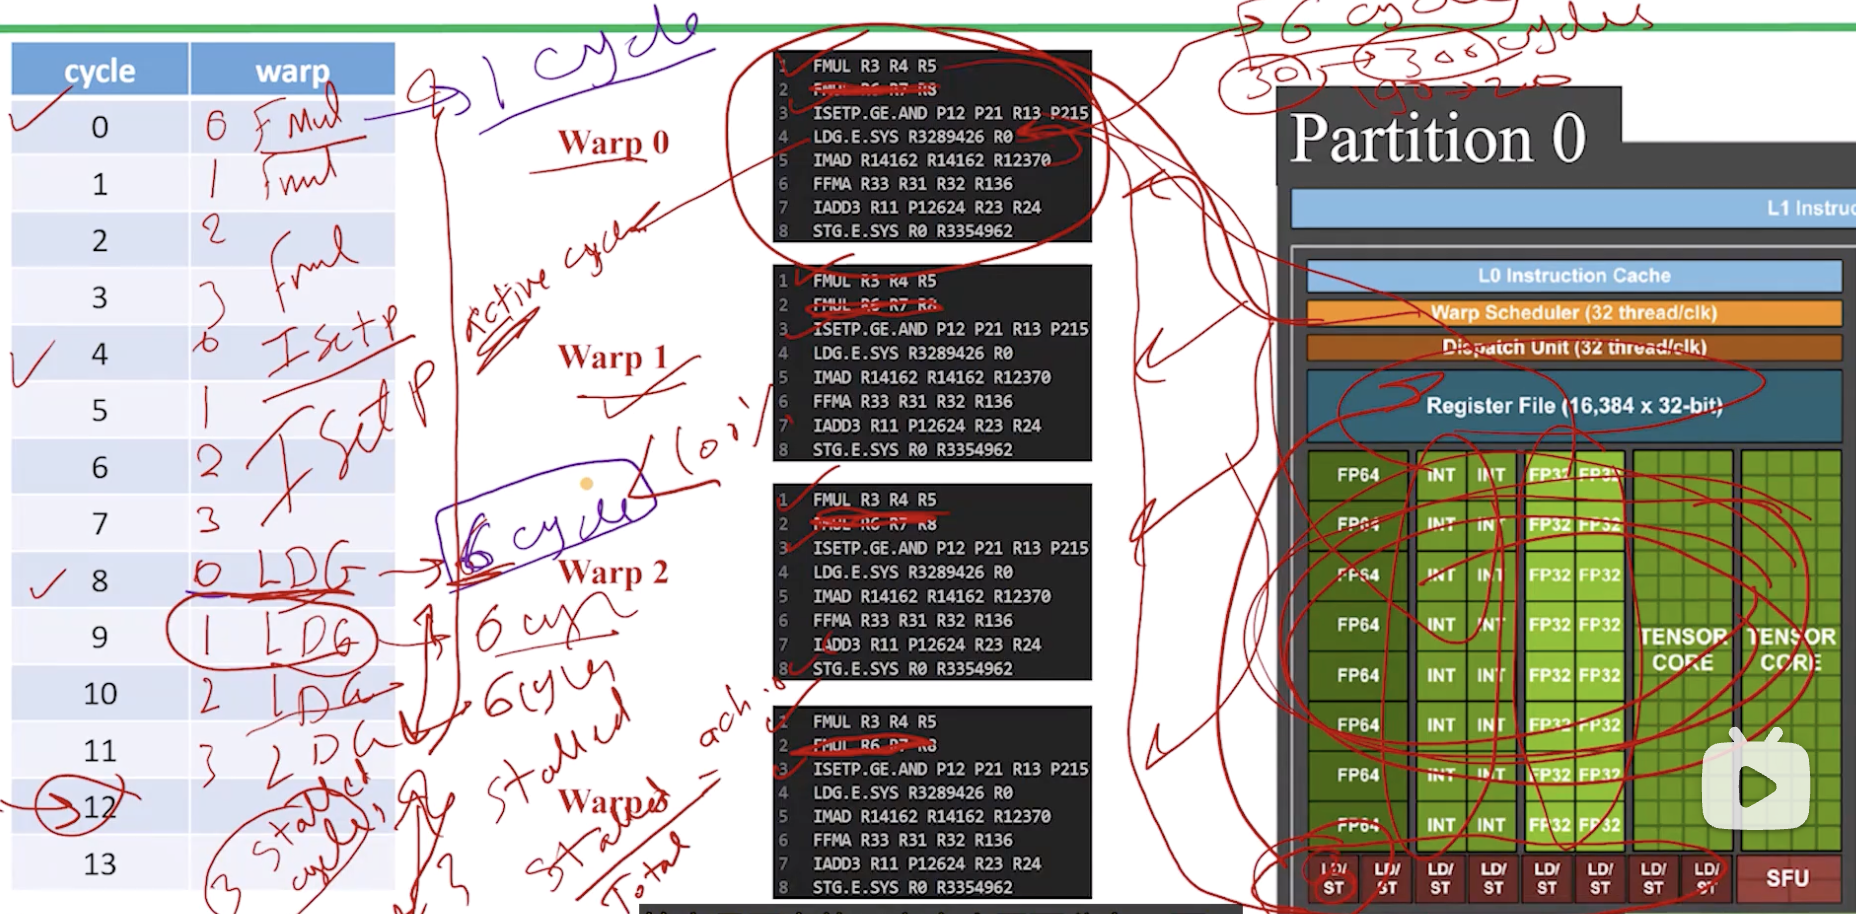
\includegraphics[width=0.75\linewidth]{resources/cuda-093.png}
    \caption{}
    \label{fig:placeholder}
\end{figure}

现在把重点转移到达到的占用率。首先回顾 GPU 的结构：一个 GPU 由多个 SM 组成，每个 SM 包含多个分区。在 Ampere 和 Volta 架构中，每个 SM 包含四个分区。这是一张仅一个分区的图片，在本章剩余内容中会用到它。

在这个层级中，应用程序在整个 GPU 上运行，块被指定在 SM 上运行，而 Warp 在分区上执行。Warp 是本章的焦点，需要来自软件的 Warp 和来自硬件的分区。调度单元负责获取就绪 Warp 的就绪指令，并将它们发送到适当的计算单元。GPU 内的每个分区包含一个调度器，它负责在每个周期分配一个 Warp 来执行。

\subsection{简化示例设定}

假设有一个应用程序，其中每个 SM 只取一个块，并且块大小是 512 个线程。这意味着块大小等于 16 个 Warp（$512/32$）。同时假设使用一个不同的 GPU，其限制是每个 SM 16 个 Warp。$16/16$ 得出的理论占用率为 100\%。

然而对于达到的占用率，存在 Warp 未就绪的情况。例如当一个 Warp 正在等待来自内存的值时，这可能需要 30 到 300 个周期不等，具体取决于访问的缓存级别。在此期间，其他 Warp 可能被调度执行。但如果所有 Warp 都遇到显著的内存请求或指令依赖，调度器可能会遇到没有 Warp 准备好执行的周期，这就引入了所谓的停顿周期（Stall Cycle）。

\subsection{场景一：无内存请求无指令依赖}

有两个场景来澄清这一点。在第一个场景中，假设没有内存请求或指令间的依赖。这里涉及两个术语：占用率和延迟隐藏，将在后面解释。

从这张图片开始，包含了某个代码应用的部分汇编指令。可以使用名为 \texttt{nvbit} 的工具获得这个指令跟踪。在 NVIDIA GPU 的情况下，汇编指令被称为 SASS 指令。可以搜索该工具以了解更多信息，同时也搜索 SASS 指令这个术语。

这张图片仅代表一个 Warp，但假设有四个 Warp。在硬件部分，假设将在一个分区上执行这四个 Warp（不是一个 SM，不是整个 GPU）。请问：每个分区利用了多个 Warp，在这种情况下有四个 Warp，能计算每个 SM 利用的 Warp 数吗？答案是肯定的。如果一个 SM 有四个分区，每个分区执行 4 个 Warp，那么每个 SM 的最大 Warp 总数将是 $4 \times 4 = 16$。

能计算理论占用率吗？理论占用率等于应用程序中使用的 Warp 数除以总数再乘以 100\%。在这种情况下，最大 Warp 数是 16，应用程序中使用的 Warp 总数也是 16，所以理论占用率是 100\%。

下面解释 Warp 调度器的功能。Warp 调度器开始与所有 Warp 对话，询问它们谁准备好执行其指令之一。假设 Warp 0 会说："是的，我准备好执行这里的第一个指令，即 FFMA（F 指的是浮点乘法）。"调度器会说是的，有就绪 Warp，它准备好执行 FFMA。调度器将获取这个指令并将其发送到所有这些核心。可能会疑惑为什么取一个指令并发送给所有这些核心，只需要一个核心？答案实际上不止一个指令，有 32 个 FFMA 指令。

为什么有 32 个指令？需要记住每个 Warp 由 32 个线程组成。这些线程执行相同的指令但处理不同的数据，这意味着这个指令后面应该跟着另一个 FFMA 指令用于第二个线程但使用不同的寄存器。对于所有 32 个线程都是如此，这就是为什么这个指令将被获取并发送到这些核心执行。在周期 0 中，拥有就绪 Warp 准备好执行 FFMA 指令。

然后在下一个周期，调度器会再次询问谁准备好执行指令。假设它们按顺序执行，Warp 1 应答并就绪，可以执行第一个 FFMA。调度器将类似于第一个 Warp 那样获取这个指令并发送到核心。对于 Warp 2 和 Warp 3 同样适用。然后这个周期将再次重复，Warp 0 将在周期 4 回复 FFMA 指令。

然后在周期 8，Warp 调度器将再次询问所有 Warp 谁就绪以及什么指令就绪。Warp 0 会说："我就绪了，有一个整数指令 ISETP。"ISETP 是一个用于比较的整数指令，它比较两个值并选择其中一个。比方说如果其中一个大于另一个，它会取第一个并存储在这里；如果不是更大的那个，它会取第二个并存储在这里。在这个例子中它是一个整数指令，调度器会获取这个指令并将其发送到整数流水线。对于所有其他 Warp 也同样适用。

同样的周期再次重复，可以说达到的占用率等于 100\%。为什么？因为每个周期都有一个 Warp 准备好执行它的指令之一。如果出于任何原因，在这些周期中的任何一个发现 Warp 都没有准备好执行，这将被称作一个停顿周期。没有 Warp 就绪意味着停顿周期，在这种情况下达到的占用率将小于 100\%。当指令间没有依赖时，达到的占用率是 100\%，等于理论占用率。

\subsection{延迟隐藏的概念}

但场景一中没有内存请求，这是一个非常简单的例子。下面解释延迟隐藏这个术语。

延迟隐藏是 GPU 相较于 CPU 的主要特性之一。在 CPU 的情况下，没有这么多计算资源，可能有 4 个、8 个或 16 个核心，这就是为什么在 CPU 的情况下没有 Warp。CPU 使用一些技术，例如乱序执行（Out-of-Order Execution）。

举例来说。假设有 \texttt{ADD R1, R2, R3}，然后 \texttt{MUL R4, R1, R5}，再假设有 \texttt{SUB R10, R11, R12}。如果关注前两条指令，可以看到这里有依赖关系：MUL 指令依赖 ADD 指令的结果 R1。

当 ADD 指令进入 CPU 执行时，下个周期不会发送 MUL 指令，因为有依赖关系。MUL 必须等待 ADD 完成然后才开始执行，在这种情况下有一些停顿周期。CPU 使用乱序执行技术：SUB 指令没有依赖，CPU 改变指令顺序使其准备好执行，当 ADD 在执行时 SUB 可以发送给 CPU 准备在下个周期执行。

这可以应用于 CPU，但在 GPU 中不需要那样。为什么？在 GPU 的情况下，大多数时候不止有一个 Warp，有很多 Warp，它们可能包含一些就绪的指令。如果这个 Warp 没有就绪（比如有依赖关系），不需要对指令进行重排序，因为可以和另一个 Warp 对话，通常可以找到一个就绪的指令。这就是所谓的通过提供大量 Warp、大量线程、大量指令在所有计算单元上执行来隐藏延迟。

\subsection{场景二：内存请求与指令依赖}

在第二个场景中，假设只有一个内存请求并且还有一个指令依赖。看看从这个地址读取值并存储到这个寄存器。假设 LDG 指令（全局内存加载）将等待来自内存的值。

在 LDG 指令和后续指令之间存在依赖关系，有一个内存请求和一个依赖。还假设有四个 Warp。假设只有一个 FFMA，在第一个周期调度器询问所有 Warp 谁就绪，第一个 Warp 用 FFMA 回复，调度器获取指令并发送。Warp 0 就绪执行 FFMA。下一个周期 Warp 1 就绪又是 FFMA，Warp 2、Warp 3 同样，前四个周期执行 FFMA，与场景一类似。

假设加载指令将消耗 6 个周期（通常实际值在 30 到 300 个周期之间，取决于访问的缓存级别：L1 缓存约 30 周期，L2 缓存约 190-200 周期，全局内存约 300 周期）。为了简单起见假设 6 个周期。

那么在周期 4 执行完 FFMA 之后，调度器再次与所有 Warp 对话。Warp 0 说准备好执行整数指令 ISETP，调度器将其带到整数单元。Warp 1、2、3 同样适用。在这里完成了 ISSUED。

调度器再次问谁就绪，Warp 0 说准备好了但现在在执行加载指令。在周期 8，加载指令将被调度器移到加载/存储单元（Load/Store Unit），而不是计算单元。加载/存储单元负责内存不同级别（L1、L2、全局内存）之间的连接。这个指令消耗 6 个周期，意味着这个 Warp 将不可用除非 6 个周期结束。

然后 Warp 调度器问第二个 Warp 准备好了吗？它说准备好执行加载指令，但这也要花费 6 个周期。Warp 2 和 3 同样加载 6 个周期。

现在在周期 12，最重要的一点是调度器将与 Warp 0 对话："准备好了吗？"Warp 0 会说："不，还没准备好。因为想执行 ISETP 指令，但这个指令依赖于从内存来的结果，现在没准备好因为加载指令还没完成。"为什么没准备好？这里只过了 3 个周期（从周期 8 到周期 12 是 4 个周期，但加载需要 6 个周期），还必须再等 2 个周期才会准备好。

调度器将询问下一个 Warp，Warp 1 也会说不可用因为加载指令需要 6 个周期还没完成。这就是为什么这里至少会有 2 到 3 个停顿周期。停顿意味着所有这些 Warp 中没有一个准备好执行任何指令，因为内存请求。

在这种情况下可能会看到一些活动周期（Active Cycle），因为在这个周期中计算单元之一是活动的，正在执行 FFMA 或 ISETP 甚至是加载。但这里有停顿的情况。将活动周期除以总周期（而不是停顿周期）将得到达到的占用率。

举一个带数字的例子。假设总共有 100 个周期，有 85 个活动周期，那么将有 15 个停顿周期。达到的占用率等于 $85 / 100 = 85\%$。

现在已知什么是达到的占用率以及它与理论占用率的区别。为什么理论占用率是 100\% 而达到的占用率是 85\%？因为理论占用率只取决于 Warp 的数量，这很容易计算，所以它被称为理论的。但达到的占用率取决于每个 Warp 指令在执行时的动态实时行为。

\subsection{Nsight Compute实测验证}

\begin{figure}
    \centering
    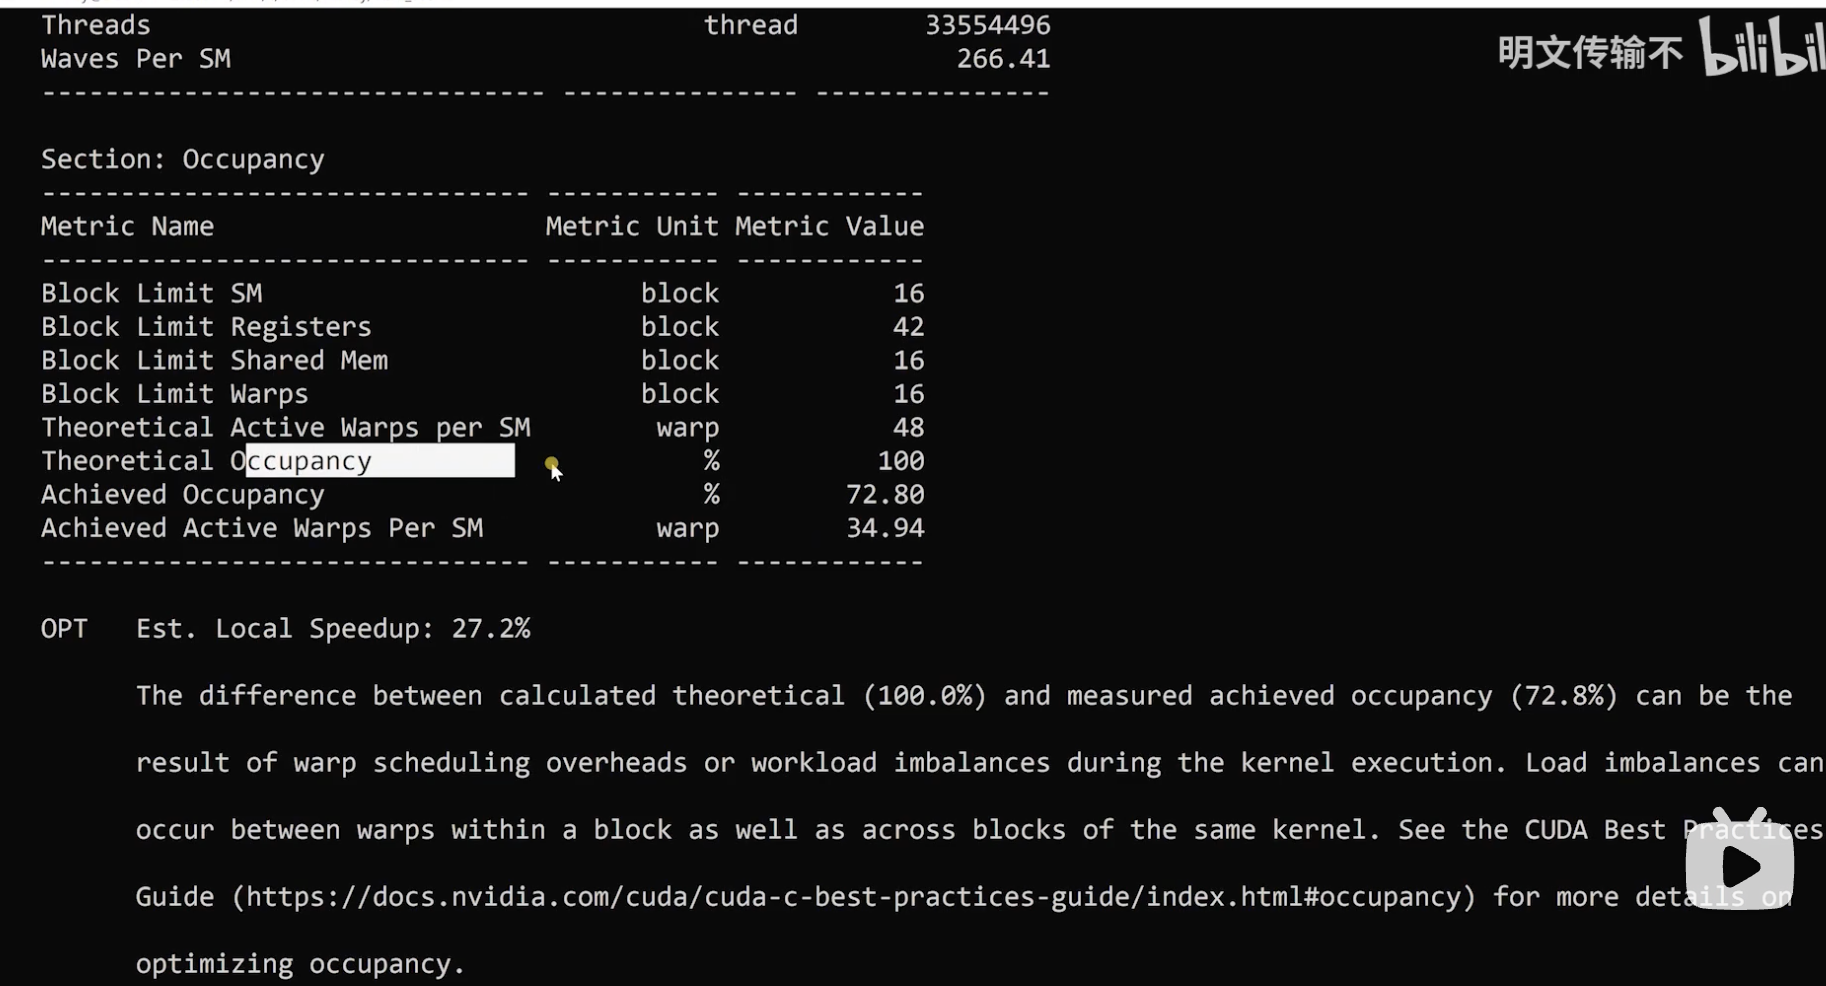
\includegraphics[width=0.75\linewidth]{resources/cuda-094.png}
    \caption{}
    \label{fig:placeholder}
\end{figure}

再次运行 \texttt{ncu ./vector\_add}。达到的占用率是 72.8\%，而理论占用率是 100\%。

达到的占用率不能通过方程计算，因为它取决于运行时执行。总的达到的占用率是由所有分区和所有 SM 上的运行时计算得出的，而不仅仅是一个分区。这里的计算仅由一个分区完成，这就是为什么这里的计算会复制到 4 个分区中的每一个，然后取平均值以获得每个 SM 的达到的占用率。然后总的达到的占用率值通过对所有 SM 的值取平均来确定：将所有 SM 的达到的占用率加起来除以 SM 的数量。一旦有了每个 SM 的达到的占用率，这个方法将应用于所有 SM，意味着将拥有等于 GPU 中可用 SM 数量的达到的占用率值。这就是计算整个 GPU 而非一个分区的达到的占用率的方法。

\subsection{为什么GPU占用率很重要？}

\begin{enumerate}
    \item 令人惊讶的是，高占用率并不总是等同于高性能，但它确实表明 GPU 资源中有很大一部分正在被利用。当看到占用率是 100\% 时，意味着许多资源将被利用。
    \item 识别和理解占用率可以帮助查明性能问题和优化机会。回顾第一个关于修改每个块线程数的例子：将每个块的线程数从 32 增加到 64 再到 96 的影响，以及对理论占用率的差异。这是其中一个例子。理解占用率将帮助查明性能问题。另一方面，低占用率表明存在瓶颈阻碍了 GPU 被充分利用。
    \item 如需进一步信息，建议访问 NVIDIA 官方文档页面。它也解释了在决定这些占用率时起作用的因素，配备了足够的细节以帮助理解理论和达到的占用率的细微差别。
\end{enumerate}


\section{每个SM分配的活跃线程块详解}

\subsection{引言：核心概念与硬件限制表}

欢迎大家。今天的文章聚焦于GPU性能分析中的一个基本概念，即每个SM分配的活跃块（Active Blocks perSM
）。这个术语不仅与占用率同等重要，而且它直接影响占用率或GPU利用率。

要完全理解这个术语，必须将注意力转向这张表格。这张展示的表格是我从A100GPU白皮书中拿来的，该表格显示了Ampere
架构的硬件限制或约束。我不会涵盖表格中的所有行，为了今天的目的我将只重点介绍四个关键行。这意味着在任何给定时间，每个SM
上不能超过32个块同时运行或并发运行。


\begin{figure}
    \centering
    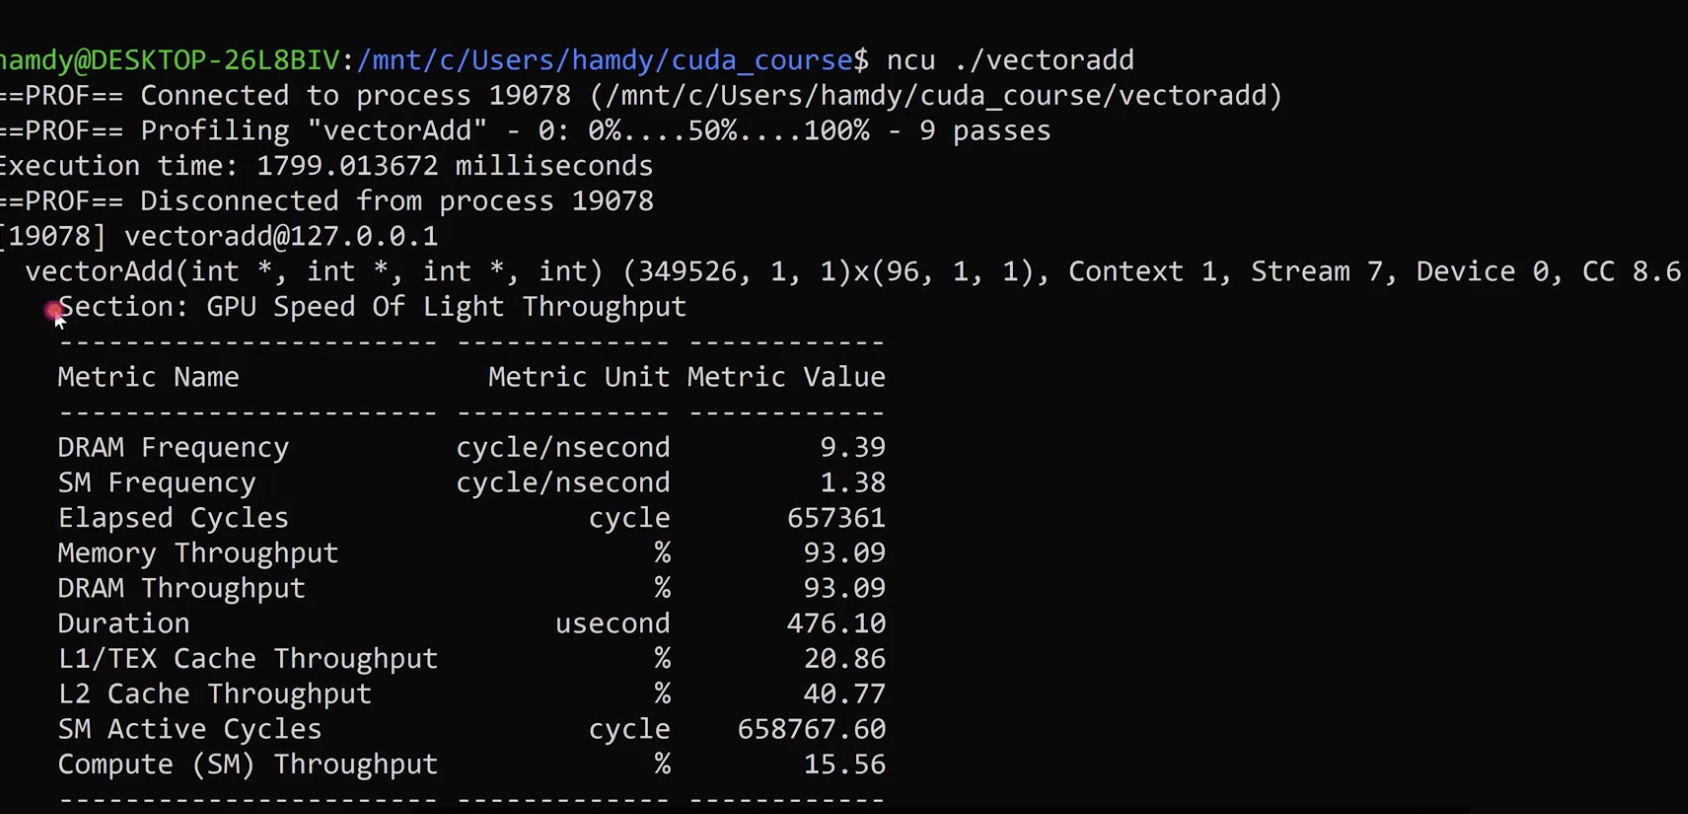
\includegraphics[width=0.75\linewidth]{resources/cuda-095.png}
    \caption{}
    \label{fig:placeholder}
\end{figure}


\subsection{四个关键硬件限制}

\subsection{每个SM的最大线程块数}

本文章中要检查的第一行是每个SM的最大线程块数，在这种情况下其值为32个块。最大值是32个块。

\subsection{每个SM的最大Warp数}

我今天想检查的第二行呈现了每个SM的最大Warp数，即单个SM上可以同时执行的最大Warp数。对于A100GPU，这个限
制是每个SM64个Warp。这意味着无论每个SM分配的块数是最大值32个块还是更少，这些块中所有Warp的总和不能超过每
个SM的最大Warp数，即64。

这是这里的主要关键点：\textbf{Warp数限制控制着每个SM可以分配多少个活跃块}。我们知道最大值是每个SM32个
块，但应用程序可能使用少于32个块，这取决于Warp数限制。我希望你把这句话记在心里，永远记住这句话。

然而如果每个块包含4个Warp，那么32个块的Warp总数将是128个Warp。为了理解这一点，让我们考虑一个例子：应用
程序每个SM分配32个块，这等于表格中提到的每个SM最大块数。但这个值128个Warp超过了表格中规定的Warp数限制，
编译器将尝试解决这个问题。

根据表格该值不应超过64个Warp，编译器会介入遵循以下逻辑：编译器理解每个SM最多可以利用32个块，然而如果每个块由4
个Warp组成，那么总的Warp数将是128。这超过了可接受的Warp数限制（而不是块限制）。编译器将决定将活跃块的数量
从32减少到16。经过这个调整，总的Warp数将变成$16 \times 4 = 64$ 个Warp。这个值落在可接受的
范围内并且没有超过Warp数限制。

\subsection{块限制Warp数（Block Limit Warp）}

如何控制每个SM分配的活跃块？这个例子揭示了一个关键概念，称为“块限制Warp数”（Block LimitWarp）。正
如这张我从NsightCompute工具分析中获取的图片所示，很明显“块限制Warp数”这个术语出现在占用率部分。这强调
了我之前在占用率文章中提到的关于占用率与每个SM分配的活跃块之间关系的观点。这个例子表明，尽管最大块限制是每个SM32个
块，但最终每个SM分配的块数受Warp数限制的约束。

\subsection{全局块分配与并发块的区别}

我想提一个关键点：可以在整个GPU上运行的最大块数非常大，可能达到数百万。你可以通过之前讨论过的CUDA运行时API来检
查这个限制。这个巨大的数字需要分布在数十个SM上。在A100GPU中我们有108个SM，这意味着有可能为每个SM分配超过
1000个块。然而这里的关键问题是：这1000个块中有多少个可以在一个SM上\textbf{并发运行}？

当我们提到每个SM 32个块的限制时，并不意味着只能分配32个块；相反意味着你可以分配超过32个，但只有32个或更少的块
会同时运行或并发运行。

\subsection{寄存器限制与寄存器溢出}

同样的原则适用于每个SM的最大寄存器数。A100 GPU中的最大值超过65000。

例如，考虑一个应用程序利用一个块，每个SM块大小为1024个线程。我们每个SM只有一个块，然而表格设定的限制仅为65536。如果每个线程需要100个寄存器，那么每个SM所需的总寄存器数将是$1024 \times 100 = 102400$
个寄存器，超过了允许的最大限制。

在这种情况下，我们不能通过减少每个SM的块数来解决这个问题，因为应用程序每个SM只利用一个块。你可以减少每个块的线程数来
解决这个问题，但如果你不这样做，那么所需的寄存器将超过允许的最大限制。

\textbf{寄存器溢出}（Register Spilling）会导致性能下降，这是因为本地内存比普通寄存器慢。这将导
致使用本地内存来存储这些寄存器的值。检查你的应用程序是否过度依赖寄存器溢出是至关重要的，你应该寻求改进应用程序的方法来缓
解这个问题。

\subsection{寄存器限制计算示例}

在这个例子中，我们需要计算每个SM分配的活跃块数。设块大小为512个线程（可配置参数），每个线程需要16个寄存器（取决于
应用程序代码，不在我们控制范围内）。

每个块所需的总寄存器数：$512 \times 16 = 8192$ 个寄存器。

在寄存器限制为每个SM 65536个寄存器的情况下，可以并发运行的最大块数
： \[\left\lfloor \frac{65536}{8192} \right\rfloor =
8 \text{ 个块}\]

这意味着尽管规定的块限制是每个SM 32个块，但在寄存器限制下将只选择8个块来并发运行。

\subsection{四重限制取最小值原则}

同样的原则适用于可用的Warp数（Warp限制）、可用的寄存器数（寄存器限制），以及表格最后一行的共享内存限制。虽然我现
在不会深入探讨共享内存约束的细节，但我们将在后面更深入地探讨这个主题。

我想解释最后一个例子，以说明Warp限制、寄存器限制和共享内存限制对每个SM分配的活跃块的影响。“分配的活跃块”指的是这
些块中有多少个可以\textbf{并发运行}，你可以为每个SM分配数百或数千个块，但并发数受限。

假设以下条件：
\begin{itemize}
    \item \textbf{块限制Warp数}: 4个块（如果使用超过4个块，将超过Warp数限制）
    \item \textbf{块寄存器限制}: 8个块
    \item \textbf{块共享内存限制}: 16个块
    \item \textbf{硬件最大块限制}: 32个块
\end{itemize}

在这四个值中，NVCC编译器将选择它们中\textbf{最小的值}。尽管块限制是32，寄存器限制是8，共享内存限制是16
，但Warp限制约束会超越它们，规定最多只能并发运行4个块。寄存器说可以运行8个，但Warp限制说不能运行超过4个。最终
值将取最小的那个值。

我想你现在可能明白了为什么我们在计算理论占用率时要取最小值。这就是为什么你需要理解“每个SM分配的活跃块”这个术语，以便
能够理解为什么在分析应用程序时要在这四个值中选择最小值。

\subsection{Nsight Compute实测验证：RTX 3090}

\begin{figure}
    \centering
    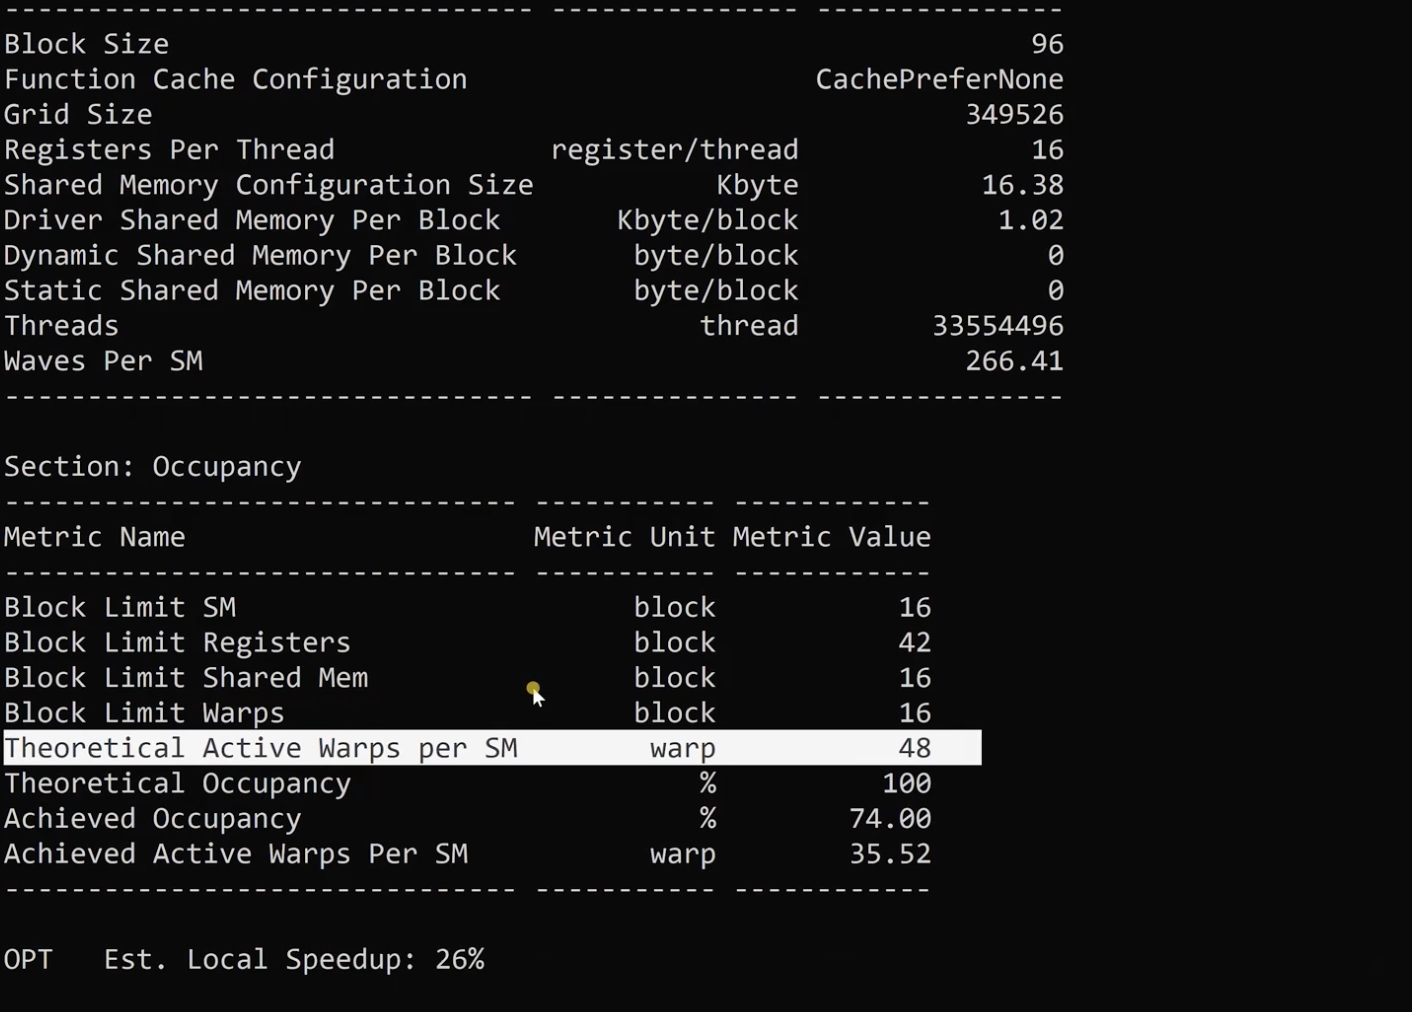
\includegraphics[width=0.75\linewidth]{resources/cuda-096.png}
    \caption{}
    \label{fig:placeholder}
\end{figure}

现在让我们再次分析向量加法应用程序。输入 \texttt{ncu ./vector\_add}（即NsightCompute）。如你所见，我们有三个部分：GPU Speed of Light、LaunchStatistics和Occupan

cy。我们需要的是占用率部分。


在这个部分内，前四个度量指标就是我们今天研究过的：
\begin{itemize}
    \item \textbf{块限制Warp数}: 16个块
    \item \textbf{块共享内存限制}: 对应值
    \item \textbf{块寄存器限制}: 42个块（今天影响较小）
    \item \textbf{硬件最大块限制}: 32个块
\end{itemize}

这四个值中的最小值是16。你可能想知道为什么是16而不是32？因为这里我是在RTX 3090GPU上解释，而不是A100
GPU。让我通过 \texttt{nvidia-smi}来检查一下，或者使用运行时API检查每个SM的最大分配活跃块数。

在这种情况下，每个SM分配的活跃块数是16个块，这就是我们用于理论占用率计算的值，我们不能并发运行超过16个块。

\subsection{理论占用率100\%的验证}

例如这里的理论占用率是100\%。为什么是100\%？我们知道块大小是96。让我们进行上一个文章中已经做过的相同计算：

\[\text{每块Warp数} = \frac{96}{32} = 3 \text{ 个Warp}\]

RTX 3090中每个SM的最大Warp数是48（我在占用率文章中解释过这个值）。如果我们有3个Warp乘以从四个值中得
到的最小分配活跃块数16：\[3 \times 16 = 48 \text{ 个Warp}\]

而在我的应用程序中我们利用了48个Warp。如果每个SM的最大活跃Warp数是48，那么：\[\text{理论占用率}
= \frac{48}{48} \times 100\% = 100\%\]

这就是为什么理论占用率是100\%。这只是理解这些参数的影响及其含义的一个例子，因为如果我们用最大值除以应用程序中利用的
值，百分比将是100\%。



\section{掌握CUDA GPU并行编程（硬件与软件）Nsight Compute入门}

本章本来应该开始讲解如何使用 Nsight Compute 工具来分析 CUDA 应用。然而开始着手做这件事时，发现了一个可能遇到的问题，尤其是使用 Windows 操作系统的话，下面解释这个问题及其解决方案。

\subsection{问题分析：ncu工具报错}

首先这是 CUDA 课程文件夹，使用 \texttt{ls} 命令来列出所有文件和文件夹。如所示，有一些 CUDA 文件，还有一些可执行文件，接下来执行这个应用——向量加法项目的可执行文件。前文已经解释过很多次了，如所示，它正确执行没有任何问题，执行时间等于 6.8 毫秒。然而当开始分析这个应用时：

如果想使用 Nsight Compute 进行分析，需要输入 \texttt{ncu}，它指的是 Nsight Compute。点击回车看看输出。如所示，有一些错误，这是第一个。此外，还有另外三个错误。

为什么 Nsight Compute 工具不工作呢？它安装在系统里了吗？答案是肯定的。当安装 CUDA 工具包时，安装了许多库和工具，其中之一就是 Nsight Compute，但这不是遇到的错误。除非在这里遇到错误说 \texttt{ncu} 命令未找到，否则不需要安装 Nsight Compute。

\begin{figure}
    \centering
    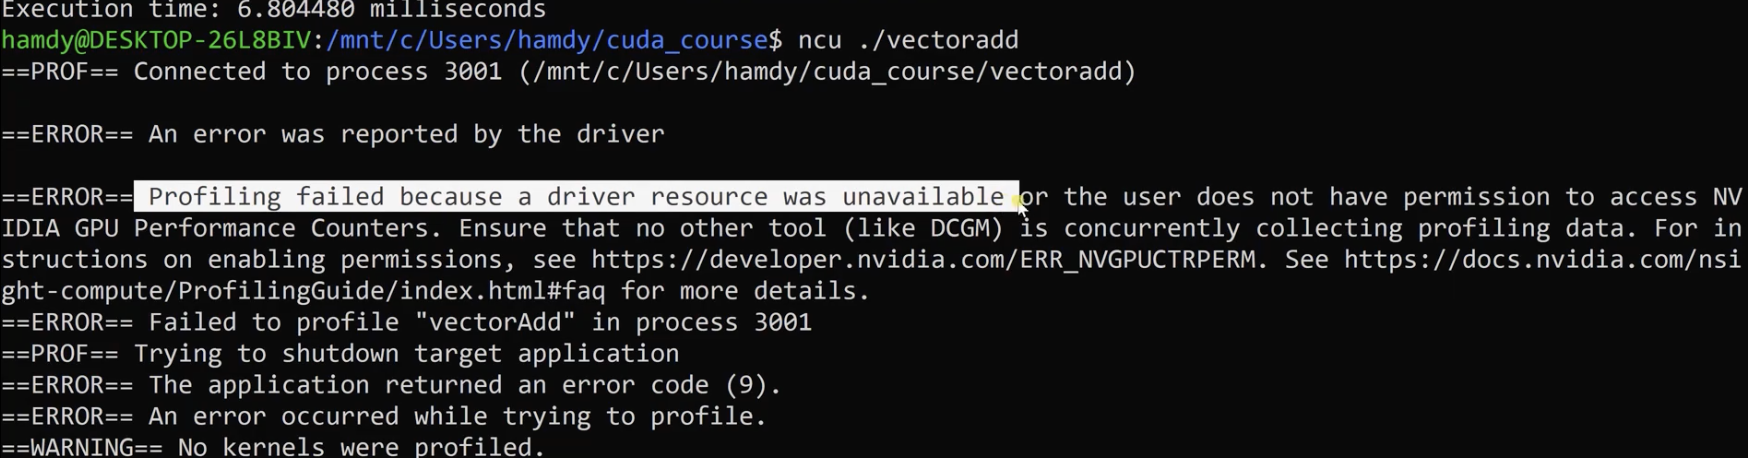
\includegraphics[width=0.75\linewidth]{resources/cuda-097.png}
    \caption{}
    \label{fig:placeholder}
\end{figure}

\subsection{GPU性能计数器权限设置}

现在检查一下这五个错误中的每一个。第一个提到驱动程序有问题，还记得这个吗？如何检查驱动程序呢？前文在解释 \texttt{nvidia-smi} 工具时提到过驱动程序。输入这个命令，看看驱动程序是否已安装。这个表格不会在这里出现。如果驱动程序有问题，这个表格将不会显示。

会遇到一个问题或错误，类似这里的情况。如所示，这里提到了驱动程序版本，甚至还有 CUDA 版本，以及 NVIDIA GeForce RTX 3090 GPU 被检测到了，驱动程序版本被检测到了，CUDA 版本被检测到了，这不是问题所在。如果这不是问题，为什么错误提到有驱动程序问题呢？这可以从第二个错误中理解。如果阅读第二个错误，就会找到答案。它说分析失败，因为一个驱动程序资源不可用，"或者"解答了问题，"或"意味着这可能是个问题，也可能不是。

那么现在检查的问题不是第一个。检查问题是否在这个部分。它说用户没有访问 GPU 性能计数器的权限。需要搜索关于 GPU 性能计数器限制的信息，以获得更多信息。下面给出解决方案：在 Windows 系统上安装 GPU 驱动程序时，它只将 GPU 性能计数器的访问权限授予管理员，而当前不是以管理员身份运行，是以普通用户身份运行。

可能会问为什么不用 sudo？因为使用 sudo 时，如所示，可能会遇到另一个问题——\texttt{ncu} 命令未找到。但确定已经安装了 Nsight Compute 工具，接下来尝试搜索 NVIDIA 面板。

如所示，右键点击并选择 NVIDIA 控制面板选项，需要几秒钟来打开一个窗口。从这个窗口，需要进入菜单并选择桌面。然后从桌面启用开发者设置，启用这个选项，将在这里显示性能计数器。请看这一部分启用。

如所示，有了开发者设置管理 GPU 性能计数器其中之一，也是这里唯一可用的。点击这里，如所示，有两个选项。第一个是仅限管理员用户访问 GPU 性能计数器，这是推荐的。但现在想允许所有用户访问 GPU 性能计数器。勾选这个选项并应用，显示器可能会闪烁。一旦选择并应用这个选项后，可以继续操作。


\subsection{重启与验证}

\begin{figure}
    \centering
    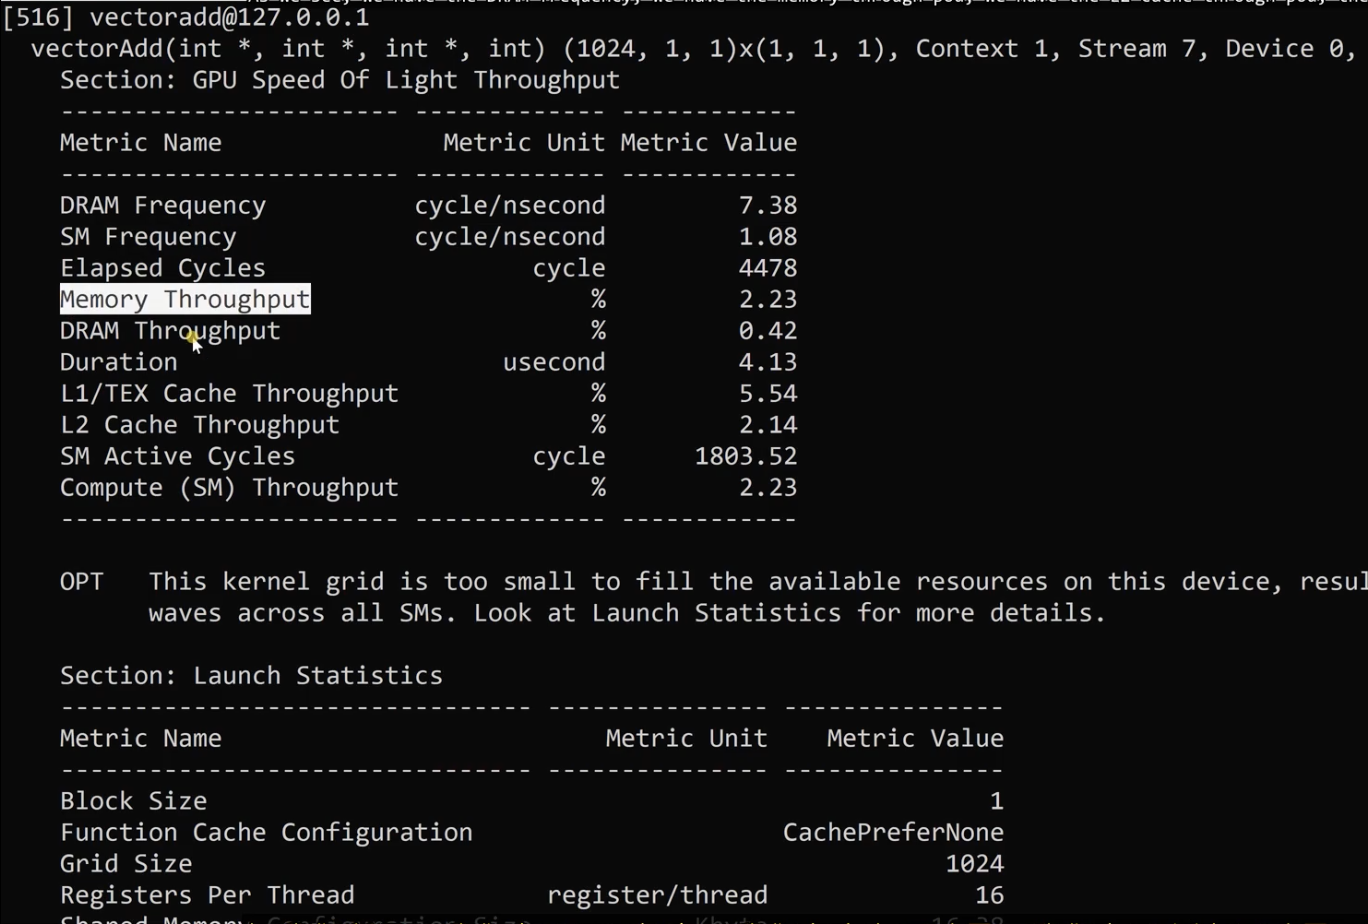
\includegraphics[width=0.75\linewidth]{resources/cuda-098.png}
    \caption{}
    \label{fig:placeholder}
\end{figure}


现在已经允许所有用户访问 GPU 性能计数器。回到这里，尝试使用命令。可以检查到错误中有一些变化。如所示，这些错误与之前的错误不同了。为了验证这一点，检查第一个错误，这里提到驱动程序，但现在这里不是关于驱动程序的。

接下来需要重启 Ubuntu 系统。输入 \texttt{sudo reboot}，然后点击回车。如果在使用 WSL（即在 Windows 上安装 Ubuntu 系统或 Linux 系统的工具），需要耐心一点。需要等待大约一分钟，然后再启动 Ubuntu 系统。等待超过一分钟后，通过输入 \texttt{wsl} 再次启动 Ubuntu 系统。等待几秒钟，然后进入文件夹。

输入 \texttt{cd cuda\_course}，然后再次运行相同的命令。如所示，得到了一些结果。有 DRAM 频率、内存吞吐量、L2 缓存吞吐量、活动周期，这些是 \texttt{ncu} 命令提供的度量指标。这里有一些配置，如块大小、网格大小，每个线程的寄存器数。还有一个名为占用率的部分，与前文讨论的占用率相关，这里有一些限制。最后有这个度量指标，即达到的占用率。本章不会解释这些度量指标，因为本章只是为了解决在 Windows 系统上运行 \texttt{ncu} 或 Nsight Compute 的问题。


\section{NVIDIA全系性能分析工具（Nsight Systems/Compute/nvprof）}

本章将深入探讨 NVIDIA 为分析和剖析 CUDA 应用程序提供的基本工具。在深入介绍这七个工具之前，需要注意的是 \texttt{nvprof} 分析工具在许多教程中被广泛涵盖，但现已被弃用。建议不要使用它，这就是它不会包含在本课程中的原因。

\subsection{CUDA-MEMCHECK与Visual Profiler}

如图所示，有七个由 NVIDIA 提供的用于分析 CUDA 应用程序的工具。从本章中的工具开始，例如 CUDA-MEMCHECK 工具。该工具有助于识别和诊断 CUDA 应用程序中的内存错误，包括越界和未对齐的内存访问错误，类似于可用于调试 CUDA 程序的 cuda-gdb 工具。CUDA-MEMCHECK 工具对于确保 CUDA 应用程序的正确性至关重要，而这反过来又会影响其性能。

本章的第二个工具是 NVIDIA Visual Profiler，简称 NVVP，以及针对 CUDA、OpenCL、Direct3D 和 OpenGL 应用程序的硬件计数器。NVIDIA Visual Profiler 是一个跨平台的性能分析工具，为开发者提供详细的时序信息。从其名称中的"Visual"一词可以知道其主要特点。该工具提供应用程序时间线和达到的占用率的图形化视图，有助于识别 GPU 核函数和内存传输中的瓶颈。

\subsection{Nsight套件三大工具}

\begin{figure}
    \centering
    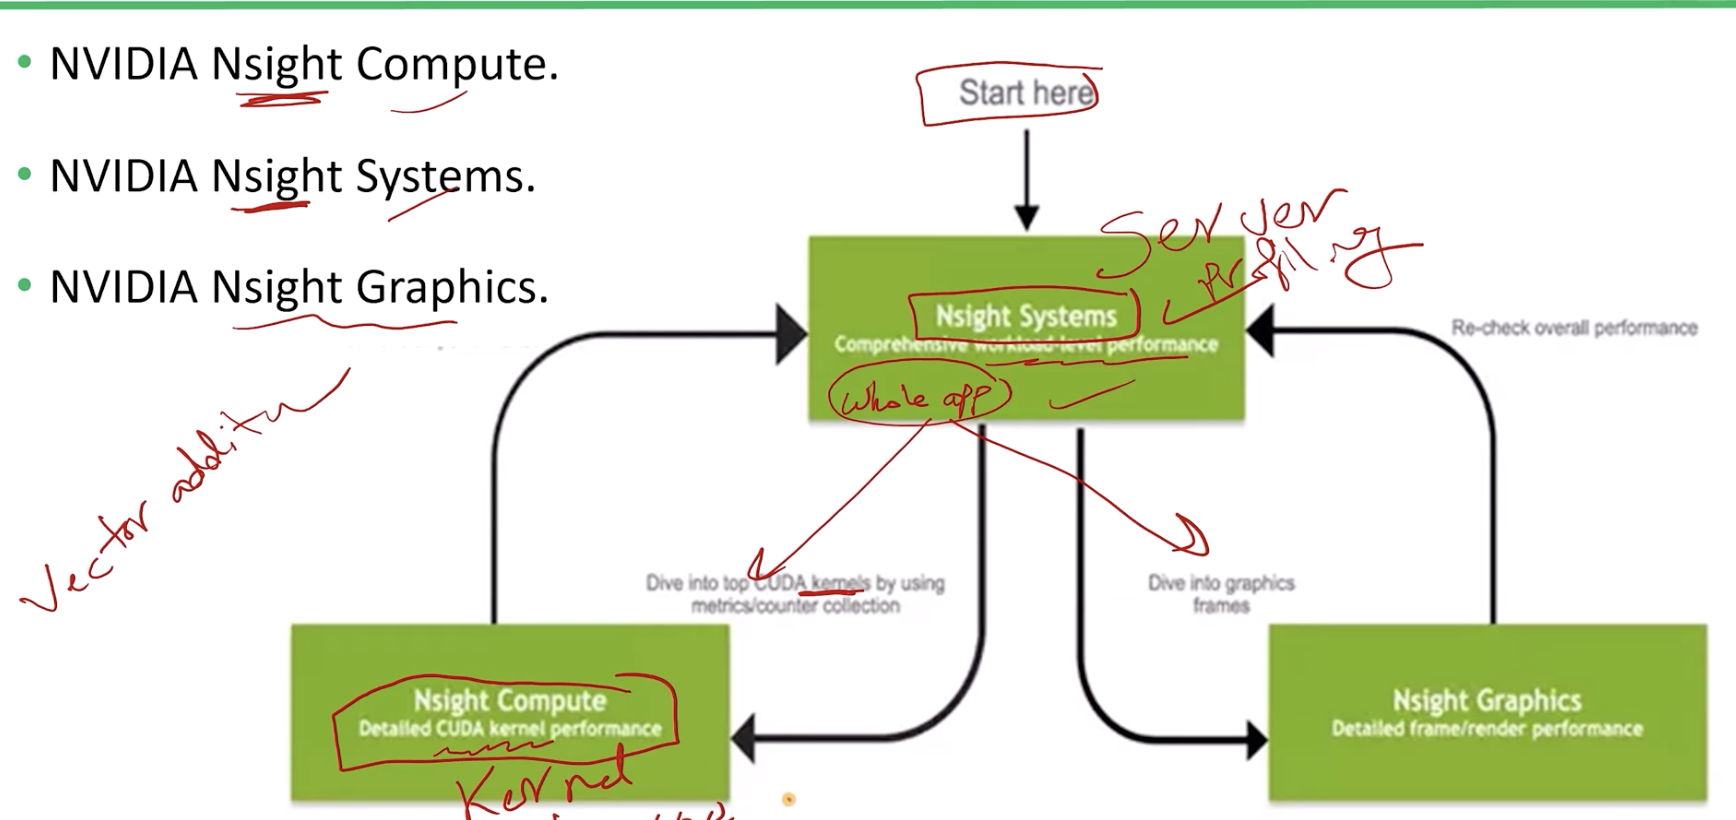
\includegraphics[width=0.75\linewidth]{resources/cuda-099.png}
    \caption{}
    \label{fig:placeholder}
\end{figure}

本章不解释所有这些工具，只专注于 Nsight 套件中三个最重要的工具：Nsight Compute、Nsight Systems 和 Nsight Graphics。这张图解释了这三个工具之间的关系。如图所示，该图从 Nsight Systems 开始，它相对于其他两个工具是外层的，这表明该工具更适合将应用程序作为一个整体来检查，而不是专注于单个核函数。这个工具即 Nsight Systems 被推荐给开发者，用于对其应用程序性能进行全系统范围的分析。当考虑到一个应用程序可能包含多个核函数，而不仅仅是一个时，这种区别就变得明显了。该工具可以可视化 CPU 到 GPU 的交互使用情况，以及 CUDA Runtime API 的性能，还能分析多节点工作负载。这就是为什么可以说 Nsight Systems 是一个服务器端分析工具，而不是客户端分析工具。这个工具就是前文分析向量加法应用程序时演示过的同一个工具。

然后为了对应用程序或工作负载中的每个核函数进行更细致的检查，Nsight Compute 是首选工具。它提供了大量针对每个核函数的详细见解和度量指标，包括全局内存、缓存、SM。甚至深入到 SM 内每个独立单元的度量指标，可用的度量指标超过 10 万个。

Nsight Graphics 提供有关图形帧和渲染性能的详细度量指标，专为图形应用程序分析和剖析的需求而定制。最后，当涉及到以图形为中心的应用程序时，Nsight Graphics 是该领域的专业工具。

在结束本章之前，留一个重要的提示。本课程中的分析重点将完全集中在 Nsight Compute 工具的使用上，可能还会涉及 Nsight Systems。


\section{错误检查API详解}

在深入探讨使用 Nsight Compute 工具分析 CUDA 应用之前，需要强调 CUDA 函数中错误检查的重要性。用一个例子来说明这一点。在进行性能分析之前，确保 CUDA 函数运行流畅且准确至关重要。在前文中提到过一个问题，即应用程序编译时没有错误，然而该应用程序却无法正确执行。经过调查，定位到了一个故障的 \texttt{malloc} 函数，原因是用于分配所需存储或所需空间的 RAM 不足。这类错误在编译期间无法检测到，在运行时也可能不会表现为可读的错误。这凸显了为所有 CUDA 函数使用错误检查的必要性。

\subsection{内存不足问题分析}

这大致可以分为两类：同步错误检查和异步错误检查。CUDA 提供了几种机制来检查其操作或函数的成功与失败。从第一类开始：同步错误检查。在 CUDA 中，像内存分配这样的操作是同步的，这意味着这些操作会阻塞主机代码的执行，直到设备完成操作。大多数 CUDA Runtime API 函数都会返回一个错误代码，这使得错误处理更加直接，因为错误会在操作完成后立即报告。可以通过检查这个错误代码来确定是否发生了错误。

现在打开向量加法代码来做一些错误检查测试。这是在添加任何错误检查指令之前，是之前章节的向量加法应用程序。首先需要测试这个应用程序是否工作正常。打开终端，列出第四节文件夹中的所有文件。如所示，有三个文件，而本章将重点关注第 2 个 \texttt{02\_enhanced\_vector.cu}。需要编译和运行，检查编译和执行步骤中是否有任何错误。从编辑器中可以看到，打开的是同一个文件。正如之前讨论的，正在使用 NVCC 编译器。\texttt{nvcc -o} 这是可执行文件的名称。以 CUDA 文件结束命令，编译时没有出现任何错误。现在运行应用程序，执行也没有任何问题。

回到这里，把这个值，也就是 32 替换成一个更大的值，$1024 \times 25$。增加每个向量中元素总数的原因是为了增加每个向量所需的总存储量，从而在给这个应用程序分配所需空间时制造一个问题。一旦出现问题，就需要通过错误检查来确切地知道问题是什么。在那之前先简化一下，把 20 这个乘数去掉。在编译和运行应用程序之前，用任务管理器检查一下电脑资源。右键点击，然后选择任务管理器。选择性能选项卡，它显示了电脑中的所有资源。从 CPU 开始到 GPU 结束，需要关注的是内存和 GPU。

原因是关注内存，因为这里有三条指令要在 RAM 中分配空间，而 RAM 在这里由内存选项卡表示。同时使用 \texttt{cudaMalloc} 函数在 GPU 中分配空间，这就是关注 GPU 的原因。

可以注意到 GPU 现在使用了大约 48\% 的资源，内存使用了 2.5 GB。也可以从图表检查这个值。具体来说关注的是专用 GPU 内存，专用 GPU 内存指的是 GPU 内部真实或实际的内存。这是因为录制程序在运行，最后一个选项卡说明这个录制程序使用了硬件加速，硬件加速指的就是 GPU 本身。需要从这里这些步骤查看 GPU 和内存。

需要计算每个向量所需的总存储量。这里就是结果，这个数字代表了每个向量中的元素总数。复制这个数字，然后写下结果代表了每个向量中的元素数量。有三个向量，那么现在需要做的是乘以 4。为什么需要乘以 4 呢？因为应该熟悉 C 语言，在 C 语言中整数值使用四字节的存储空间，因为这些元素中的每一个都包含一个整数值。需要乘以 4 来得到每个向量所需的总字节数。但现在想以 GB 为单位计算，而不是字节。然后再除一次转换成 MB，除以 1024 转换成 KB。再进行一次转换变成 GB。如所示，每个向量将使用 4 GB 存储空间。因为有三个向量，所以将使用 12 GB。现在需要再次检查资源，GPU 现在使用了 2.5 GB，当运行这个正常的应用程序时，这个值应该从 2.5 增加到大约 14 或 15 GB。

来编译。编译时出现了一些警告，需要处理警告，因为它可能在运行时、在执行时造成问题。这不是编译时的问题。现在可以执行，编译已经完成了，但在执行时应用程序可能工作也可能无法正常工作。先关注第一个问题。它指出问题从这里这部分开始。如前所述，第十七行有个问题。读一下警告本身，它说整数转换导致截断。回到应用程序，每当看到截断部分，就应该知道这个值太大了，无法存储在分配的空间里。第十七行有一个整数值，叫做 \texttt{size}，这个变量应该存储乘以 4 字节之后的结果。取 \texttt{size}，它代表这个数字，然后乘以四字节，结果将存储在这个变量中。这里的结果太大了，无法只存储在四字节中，需要超过四字节。这就是为什么需要写 \texttt{long}，而不是 \texttt{int}。然后编译，如所示，现在没有问题或警告了，然后运行。当代码应用程序正在执行时，可以检查专用 GPU 内存，它正从 2.5 增长到 15，大约 14.7 左右，GPU 内存会出现一个峰值。

\subsection{同步错误检查实现}

现在没有问题，想把应用程序所需的空间增加到一个很大的值。可能会想错误检查在哪里？大到无法装入专用 GPU 内存，甚至共享 GPU 内存。因为如果使用例如 30 GB，那么将用掉全部 24 GB 的专用内存和 6 GB 的共享内存。想增加更多，把这个值乘以 20。如果把这个值乘以 20，那么每个向量需要 80 GB。需要三个向量乘以 80 GB，这个值将大到无法放入 CPU 的 RAM 内存，甚至 GPU 内存。现在编译看看一些其他的警告。如所示，有更多警告。从第十七行开始还是同一行。因为这里的乘法不能以这种方式进行，所有这些值 1024 都是整数。但当乘以另一个 20 时，这个值将无法装入一个整数。也许 \texttt{long} 可以，\texttt{long} 足够了，但它不足以进行乘法运算本身。需要做的是复制这部分，并定义一个空间足够的变量。写 \texttt{long}，但因为 \texttt{long} 可能还不够，所以再写一个 \texttt{long}，以确保分配超过八字节。然后写等于，加上 \texttt{LL}。因为如果去掉这个 \texttt{LL}，那么就是在整数乘整数乘整数，结果应该是 \texttt{long}。这里的 \texttt{L} 指的是需要对 \texttt{long} 值进行乘法，而不是整数。但如果乘两个值，在最终值存储到这个 \texttt{size} 之前，它不足以存储在整数值中。这就是为什么如果看警告，会在其他指令上也有警告。比如第 28 行，看 for 循环，不能在这里乘这些值，因为它们现在被定义为整数。当写 \texttt{LL} 时，意味着是在乘 \texttt{long} 值，而不是整数值。然后编译并运行。

如所示，遇到了段错误。在这种情况下，知道问题所在，这个应用程序需要的空间超过了 CPU 的 RAM 和 GPU 专用内存的可用空间。但如果有一个应用程序在输出中给出了段错误，但不知道所需空间，这就是为什么需要错误检查。需要为这三个函数，也就是 \texttt{cudaMalloc} 内存分配函数添加一些错误检查。复制指令，为这三个函数放在这里。顺便说一下，需要对 \texttt{cudaMemcpy}、\texttt{cudaEventRecord}、核函数启动等做同样的事情，这里只是把这些作为例子。这只是错误对象的声明，这个对象将用于存储每个 CUDA 函数的错误。这就是为什么这个变量或对象的类型是 \texttt{cudaError\_t}，这是 CUDA 编程中的另一种结构。需要再次写上 \texttt{error =}。如前所述，每个 CUDA 函数都会提供一个错误。这个错误随后可以被检查，以确切地知道执行这个函数的问题是什么。取这个函数的输出，并将其存储在错误对象中，然后测试这个错误是否不是 \texttt{cudaSuccess}。如果不是成功，那么就有问题。需要打印这个错误。如所示，使用了 \texttt{fprintf}，但这里的错误值不是字符串值，它更像是 ID 号之类的东西。使用另一个 CUDA API 函数叫做 \texttt{cudaGetErrorString}，它接收错误 ID 并返回对应于该 ID 的字符串。这就是为什么对所有 CUDA 函数重复相同操作，并且应该对此应用程序中的其他 CUDA 函数做同样的事。

现在保存、编译和运行。同样的问题，没有从添加到应用程序的错误检查指令中得到任何指示。原因是如果在为 GPU 内存分配之前，先为主机内存分配了空间——\texttt{malloc} 和 \texttt{cudaMalloc}——输出中的段错误出现在 \texttt{malloc} 这里，而不是 \texttt{cudaMalloc}。而且没有为 \texttt{malloc} 做错误检查。需要把这些指令向下移动。现在在为 CPU 或主机的 RAM 分配空间之前，先在 GPU 中分配空间。在这种情况下，如果 \texttt{cudaMalloc} 无法在 GPU 中分配所需空间，应该能看到错误检查的输出。

编译并运行，在运行时看看 GPU 资源会发生什么。如所示，可以检查专用值。因为需要 80 GB，编译器现在正尝试分配全部的 24 GB 专用 GPU 内存，然后尝试增加共享 GPU 内存。编译器正尝试分配第一个向量的空间。但这两者都不够，所以会看到一些峰值，它尝试然后失败，如此反复。最终编译器会说"无法为第一个向量分配空间"，它会为第二个向量 B 和第三个向量 C 做同样的事。从这部分可以看到，"未能分配设备内存不足"，这是这条指令的结果。分配内存失败原因就是内存不足。一旦完成了 GPU 的分配，无论是成功还是失败，将使用这些指令为主机端分配空间。没有足够的空间来分配所需的存储，这些指令也应该会失败，这就是为什么也有一个段错误。但在尝试先在 GPU 中分配之后，这就是它的重要性。这就是错误检查在 CUDA 应用程序中的使用方式，它给出一些指示，确切地指出问题在哪里。特别是如果有一个由他人设计的应用程序，而正试图开发或增强它，错误检查就是这样工作的。

回顾本章开头提到的内容，错误检查有两类：同步和异步错误检查。对于同步错误检查，GPU 任务、GPU 函数或 GPU 操作会阻塞主机执行任何其他指令，直到 GPU 任务完成其执行。它将在这里被阻塞，直到 \texttt{cudaMalloc} 完成其执行。例如，如果编译器执行到这里的第 27 行，那么它将停在这里。在执行中编译器将尝试为向量 A 分配空间，但它不会在完成向量 A 的分配之前尝试为向量 B 分配。完成向量 A 的分配，然后进入向量 B 的下一步，无论失败还是成功都没问题。一旦完成向量 B 进入第三步，以此类推。正如所示，现在正尝试为向量 B 分配。完成了向量 A 的步骤，它失败了，但没问题。这就是同步操作的含义。这就是为同步操作使用错误检查的方式：一个错误对象使用这条指令，然后读取同步函数的输出，然后检查该错误是成功还是失败。如果操作失败，那么需要打印错误。

\subsection{异步错误检查}

\begin{figure}
    \centering
    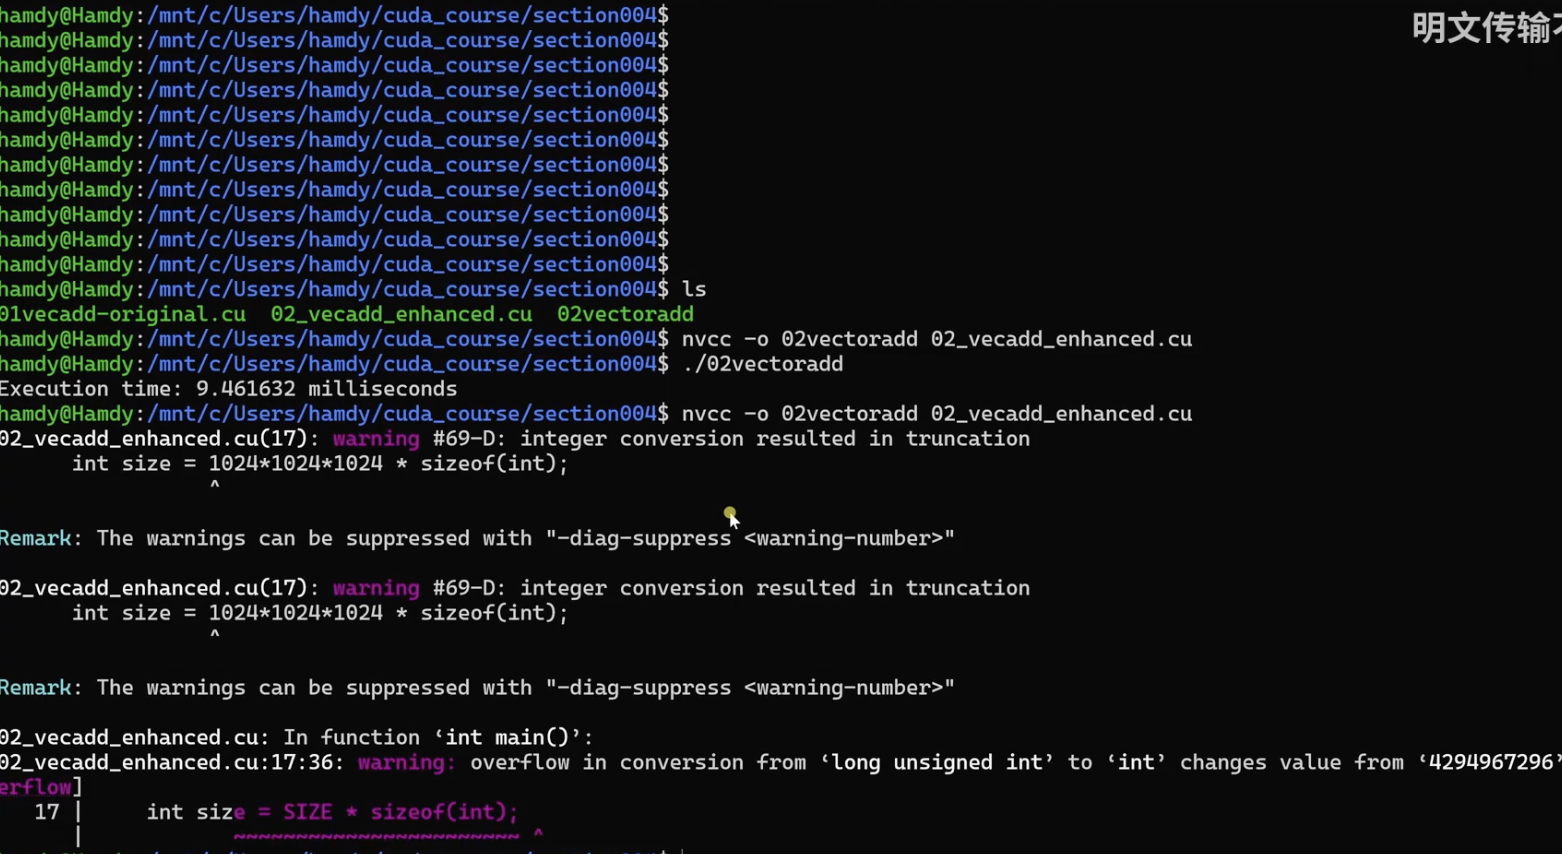
\includegraphics[width=0.75\linewidth]{resources/cuda-100.png}
    \caption{}
    \label{fig:placeholder}
\end{figure}

然而异步类型不同，因为异步类型在这里有 CUDA 启动函数代表，不会阻塞主机端或 CPU 执行下一条指令。这就是为什么如果不在这里放一个 \texttt{cudaDeviceSynchronize} 函数，执行 \texttt{cudaMemcpy}，可能会在执行完成之前复制结果。因为编译器不会停在这里，编译器将启动 GPU 核函数，然后进入下一条指令，这与在 \texttt{cudaMalloc} 函数中发生的情况不同。这就是为什么有不同的方法来检查异步操作的错误。这样做的方式就是使用一个叫做 \texttt{cudaGetLastError} 的函数。需要写一些像那样的东西，复制并把它放在这里。如所示，并不直接来到 GPU 任务本身写 \texttt{error = CUDA 函数} 或 \texttt{CUDA 启动}，不像之前做的那样。为什么？因为编译器不会停在这里，直到这个函数完成并返回一个错误存储在这里，它不会停在这里。这就是为什么不需要存储核函数执行的输出。相反，使用 \texttt{cudaGetLastError} 这个 CUDA Runtime API 函数。需要获取最后一个错误，它将存储在内存中的某个地方。而这个错误应该是 GPU 执行的最后一个函数的错误，在这种情况下就是向量加法函数。有两种不同的方法来处理这两类错误。同步错误，使用上面的方法；异步错误，使用 \texttt{cudaGetLastError} 方法。

\subsection{错误检查宏封装}

\begin{figure}
    \centering
    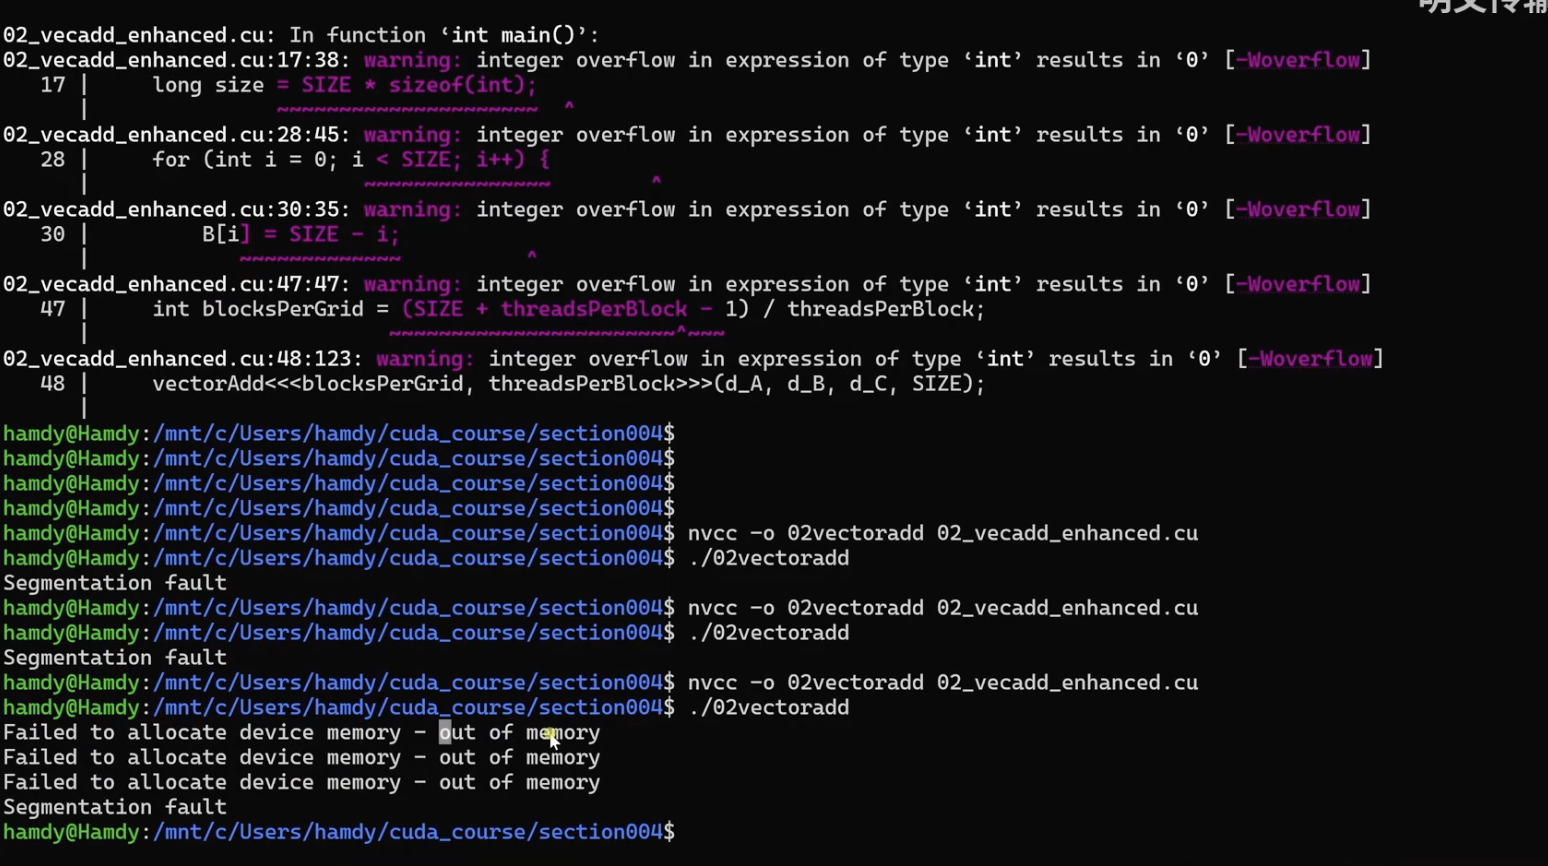
\includegraphics[width=0.75\linewidth]{resources/cuda-101.png}
    \caption{}
    \label{fig:placeholder}
\end{figure}

这里提一下，这三条指令在代码中重复了很多次。如所示，这里有这三条指令，这里也是同样的三条指令，这里也有。如果对所有 CUDA 函数使用错误检查，应该会看到它们在 \texttt{cudaMemcpy} 这里这两条函数以及 \texttt{cudaEventRecord}、用于输出的 \texttt{cudaMemcpy} 等等。这三条指令将在应用程序中重复多次，而没有必要。可以复制这部分，展示如何做到这一点。需要把这三条指令放在一个宏或一个函数里，然后在需要的时候调用它。如所示，有几行中有两个部分。第一部分是定义一个名为 \texttt{CUDA\_CHECK\_ERROR} 的宏。这个宏调用了一个名为 \texttt{cudaAssert} 的函数。\texttt{cudaAssert} 是一个函数，如所示，它接收一个来自 CUDA Runtime API 函数的错误作为输入，接收执行一个 CUDA 函数后返回的错误，然后检查错误是成功还是失败。如果成功，那么什么都不做。如果不成功，如所示，需要打印错误。但如果看这里的第一个关键字，会发现它叫做 \texttt{inline}。\texttt{inline} 指的是将这些指令内联到另一个代码中。这里不是一个分支，不是另一个函数，只是组织一下。需要复制 \texttt{CUDA\_CHECK\_ERROR}，并把它放在需要的地方。每当看到 \texttt{CUDA\_CHECK\_ERROR} 时，就是在调用 \texttt{cudaAssert}。而当调用 \texttt{cudaAssert} 时，并不是在执行另一个函数，只是复制这些指令，并把它们放在看到 \texttt{CUDA\_CHECK\_ERROR} 的任何地方。

编译并运行。不打算对所有函数都这样做，只是做一个示例。现在会看到区别，编译器正在尝试为第一个向量分配空间。看输出。如所示，看到一个叫做"GPUAssert: Out of memory"的输出，这发生在第 37 行。这就是在输出中看到的 GPUAssert。有 \texttt{\%s}，它对应错误本身，这就是为什么这里有错误本身，也就是内存不足分配。然后有文件名，也就是 \texttt{02\_enhanced\_vector.cu}。然后有行号，也就是 37。去看看 37 行，正确。但是为什么在这种情况下，没有看到三次向量 B 和向量 C 的失败？只看到向量 A 失败。因为如果看这里的 \texttt{cudaAssert}，会看到使用了 \texttt{exit}。这是因为如果无法为向量 A 分配空间，在没有足够空间的情况下，为什么要继续执行过程呢？需要退出，不需要执行那些不能正常工作的东西。在后续项目中，将使用这种错误检查方法，但不会再解释。这就是为什么需要按顺序观看所有章节。因为在每个章节中，都建立在之前解释的内容之上。

可以为异步操作做同样的事。复制这部分，来到这里。这是用于同步 CUDA 操作的，这是用于异步 CUDA 操作的。可以注意到区别，这里的 \texttt{cudaGetLastError} 函数在同步类别中没有。需要复制宏和 \texttt{cudaKernelAssert} 的定义。复制宏名，然后到这里用于核函数启动，但不需要写类似于 \texttt{error = 某物} 的东西，因为编译器不会停在这里。在完成之后，需要写一些类似那样的东西。在编译之前，把这个值减小到比如 32，以确保它在没有任何问题的情况下运行。现在执行完成没有任何问题。

以上就是关于错误检查的全部内容。通过本章的内容，应该理解了错误检查的重要性，以及如何将其用于不同的代码函数。在后续项目中，将使用错误检查而不再进行解释。


\section{命令行模式下的 Nsight Compute 性能分析}

\section*{前言}
欢迎大家。在今天的文章中，我将解释如何使用 \textbf{Nsight Compute} 工具来分析任何 CUDA应用
程序，该工具由 NVIDIA 提供。不过在文章开始前，我想先说明一点：任何公司的性能分析工具都应提供两种分析方法。

\begin{enumerate}
    \item \textbf{命令行分析 (CLI Profiling)}：正如我们这里看到的，我们可以使用一些命令来收集特定指标以评估 CUDA 应用程序的性能。
    \item \textbf{图形用户界面分析 (GUI Profiling)}：今天我将从第一种方法即命令行分析开始。在另一个文章中，我将详细讲解 GUI 分析。
\end{enumerate}

这两种方法都非常重要。有时你可能只需要收集几个指标来评估特定硬件单元的性能，在这种情况下，最佳选择可能就是命令行分析。但
如果你想进行深入的性能评估，最好使用GUI 分析，因为它可以为你提供诸如性能屋顶线分析 (RooflineAnalysis)、图表以及每个硬件单元的利用率等信息。


\subsection{文档与基础命令}
像我们通常做的那样，我将打开文档先大致了解一下命令行分析。你需要做的就是搜索 ``Nsight ComputeCLI''
并打开第一个链接。该网页包含了关于 Nsight Compute 命令行分析你需要知道的一切。

基础命令如下：
\begin{lstlisting}
ncu --set full -o profile ./my_cuda_app
\end{lstlisting}
如果你正在使用 MPI，你可以针对特定进程或者针对所有进程进行分析。此外，你还可以指定输出文件、分段文件夹，或过滤想要分
析的核函数(Kernel)。


\begin{figure}
    \centering
    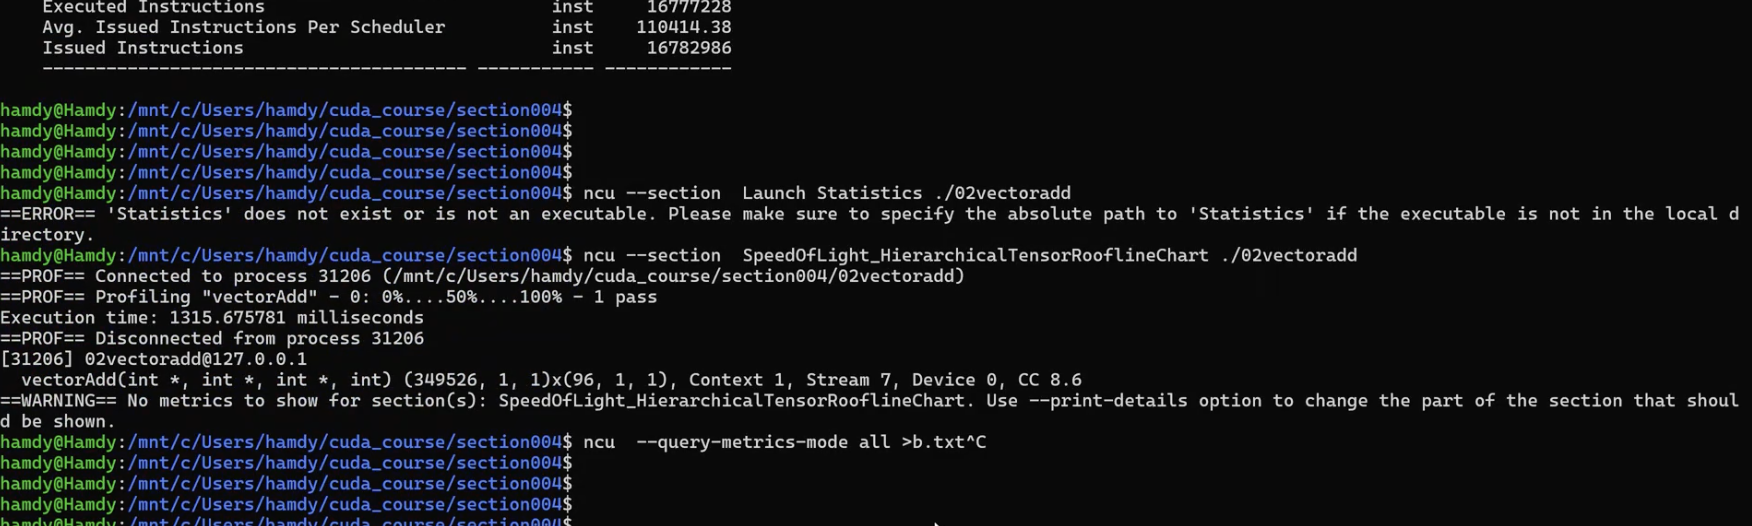
\includegraphics[width=0.75\linewidth]{resources/cuda-102.png}
    \caption{}
    \label{fig:placeholder}
\end{figure}

\subsection{分段 (Sections)}
Nsight Compute 将分析数据组织为不同的``分段''。当我们运行最简单的 \texttt{ncu}命令时，默
认会显示四个分段：
\begin{enumerate}
    \item \textbf{GPU Performance Ceiling (GPU 性能上限)}：显示 GPU 中不同单元的吞吐量信息。
    \item \textbf{Launch Statistics (启动统计)}：包含 DRAM 吞吐量、L1 和 L2 缓存吞吐量、流式多处理器 (SM) 利用率等。
    \item \textbf{Occupancy (占用率)}：包含块大小、网格大小、每个线程的寄存器数量、每个 SM 使用的共享内存大小等。
    \item \textbf{GPU and Memory Workload Distribution (GPU 与内存工作负载分布)}：显示理论占用率与实际占用率（例如本例中实际占用率为 81\%），以及 DRAM、L1、L2 缓存等的活跃周期数。
\end{enumerate}

Nsight Compute 实际上包含约 23 个分段（从 ID 4 到 27）。在命令行中，我们需要使用分段的标识符
(ID) 而非显示名称。例如，若只想查看``Launch Statistics''，可使用：
\begin{lstlisting}
ncu --section LaunchStats ./my_cuda_app
\end{lstlisting}
其他分段还包括 NVLink 通信统计、调度器统计 (Scheduler Stats)、线程束状态统计 (WarpState Stats) 等。


\subsection*{分析建议与警告}
Nsight Compute 有时会提供建议或警告。例如提示``可选指标无法找到''，这可能是因为当前 GPU架构不支持
该指标。另外，工具可能会给出停顿原因分析，例如：``平均而言，此核函数的每个线程束因等待记分牌依赖(ScoreboardDependency) 而停顿了 111个周期''。理解这些信息需要结合总周期数来判断瓶颈严重程度。


\subsection{指标 (Metrics)}
Nsight Compute 包含海量指标（约 10 万个）。为了高效使用，需掌握其命名规则。

\subsection{指标命名结构}
指标名称通常遵循以下格式：
\begin{center}
    \texttt{<硬件单元>\_\_<指标描述>.<聚合方式>}
\end{center}

\begin{figure}
    \centering
    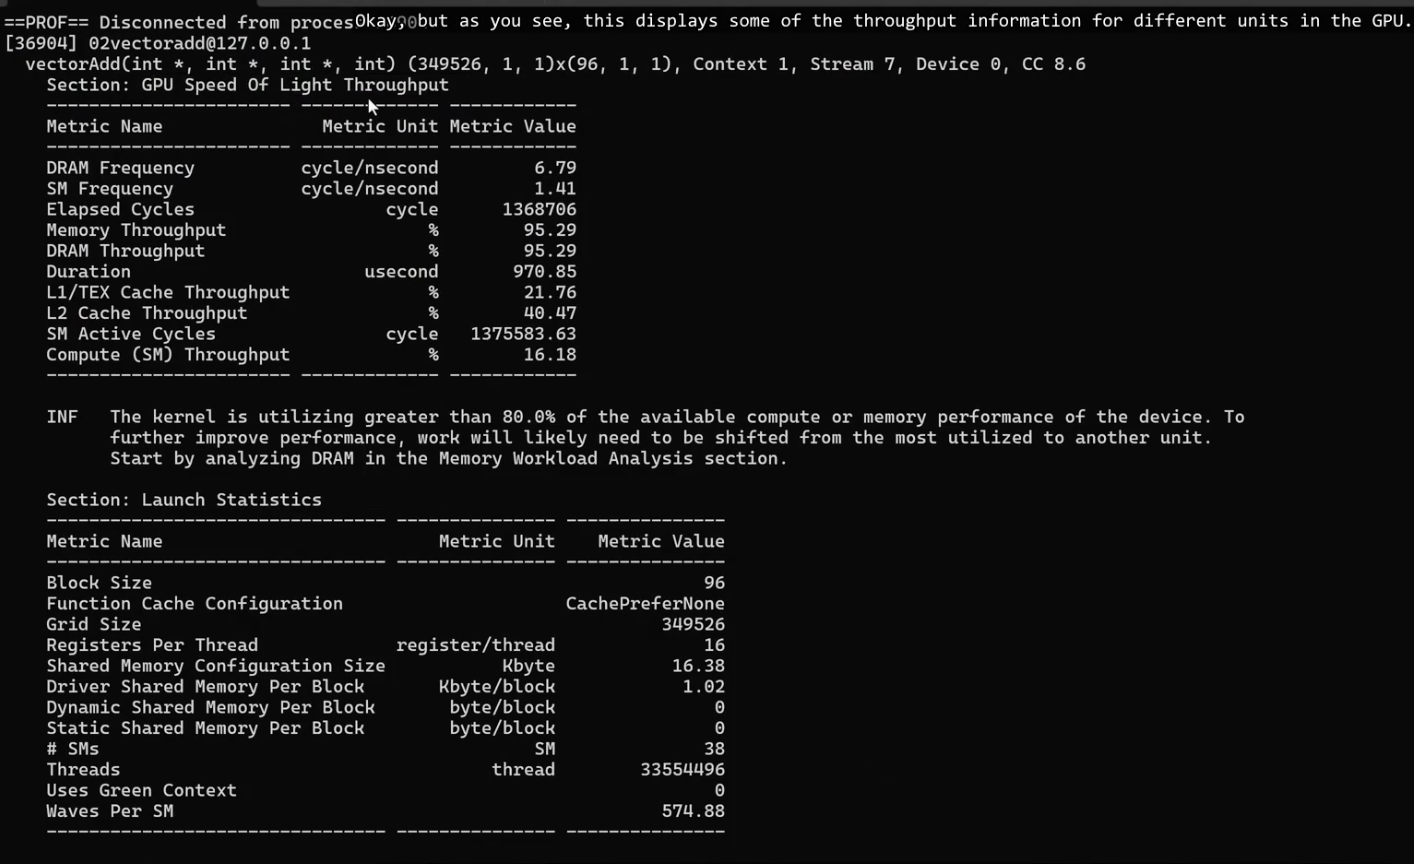
\includegraphics[width=0.75\linewidth]{resources/cuda-103.png}
    \caption{}
    \label{fig:placeholder}
\end{figure}

\subsection{硬件单元前缀}
双下划线之前的部分定义了被分析的硬件单元：
\begin{itemize}
    \item \texttt{dram}: 设备内存 (DRAM)
    \item \texttt{l1tex}: L1/纹理缓存
    \item \texttt{lts}: L2 缓存 (Level Two Slice)
    \item \texttt{sm}: 流式多处理器 (Streaming Multiprocessor)
    \item \texttt{gpu}: 整个 GPU
\end{itemize}

\subsection{聚合方式后缀}
点号 (\texttt{.}) 之后的标识符表示数据的聚合方式：
\begin{itemize}
    \item \texttt{.min}: 所有 SM 中的最小值
    \item \texttt{.max}: 所有 SM 中的最大值
    \item \texttt{.avg}: 所有 SM 的平均值
    \item \texttt{.sum}: 整个 GPU 的总和
\end{itemize}

\noindent \textbf{重要技巧：} \texttt{.sum} 是基于最大值计算的，而非平均值。即：$\text{Sum} = \text{Max} \times \text{SM\_Count}$。如果在命令行中省略点号及后缀（例如只写 \texttt{smsp\_inst\_executed}），工具将自动收集该指标的所有聚合类型（avg, max, min, sum）。
\subsection{常用指标示例}
\begin{itemize}
    \item \textbf{L1 缓存命中率}: \texttt{l1tex\_hit\_rate}
    \item \textbf{DRAM 访问字节数}: \texttt{dram\_bytes.sum}
    \item \textbf{扇区数量}: NVIDIA GPU 中每个扇区 (Sector) 为 32 字节。相关指标如 \texttt{dram\_sectors.read.sum}。
    \item \textbf{指令执行数}: \texttt{smsp\_inst\_executed.avg} (SM 内执行的平均指令数)。
    \item \textbf{管道利用率}: 可搜索 \texttt{pipe\_lsu} (加载存储单元)、\texttt{pipe\_tensor} (张量核心)、\texttt{fp16} / \texttt{fp64} 等。
\end{itemize}

\subsection{实战应用与导出}
\subsection{收集特定指标}
我们可以使用 \texttt{--metrics} 参数收集指定指标：
\begin{lstlisting}
ncu --metrics l1tex__hit_rate,smsp__inst_executed ./02_vector_add
\end{lstlisting}
如果 L1 命中率为 0\%，说明所有内存操作都访问了全局内存，这是严重的性能瓶颈，需要优化数据局部性。

\begin{figure}
    \centering
    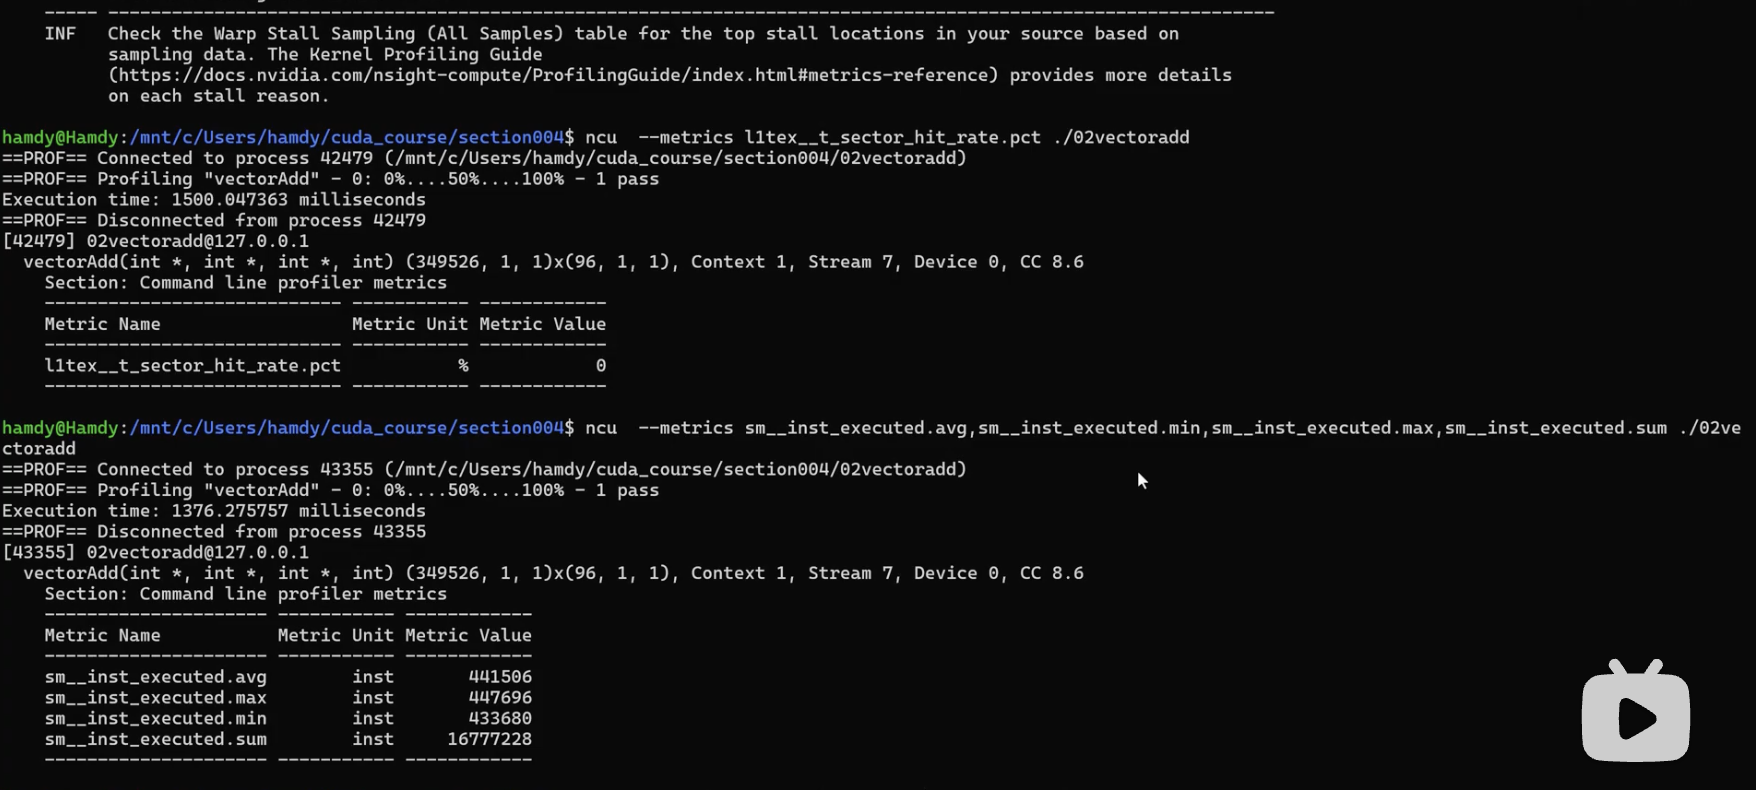
\includegraphics[width=0.75\linewidth]{resources/cuda-104.png}
    \caption{}
    \label{fig:placeholder}
\end{figure}

\subsection{使用正则表达式过滤}
若要分析特定硬件单元的所有指标，可使用正则表达式：
\begin{lstlisting}
ncu --metrics ".*shared.*" ./02_vector_add
\end{lstlisting}
这将筛选出所有包含 ``shared'' 的指标（如共享内存相关指标）。

\subsection{导出结果}
可以将分析结果导出为 CSV 文件以便在 Excel 中查看：
\begin{lstlisting}
ncu --metrics smsp__inst_executed --csv --log-file result.csv ./app
\end{lstlisting}
导出的表格包含指标名称、单位、以及各聚合方式对应的数值。

\section*{结语}
今天我们学习了如何使用 Nsight Compute命令行工具进行基础性能评估，包括分段的选择、指标的命名规则解析以及结
果导出。在后续文章中，我们将应用这些知识，通过特定指标深入分析代码，例如探究块数和线程数对核函数执行时间及周期数的具体影
响。



\section{图形化Nsight Compute使用}

在前文中，讨论了 Nsight Compute 工具的命令行分析。其中提到有两种方法来分析任何 CUDA 应用程序。第一种是使用命令行分析，前文已经讨论过了，其中讨论的一些分析内容是本节所需要的。第二种方法是使用 Nsight Compute 工具的图形用户界面，这就是本章的主要内容。将探索 Nsight Compute 的图形界面，即 GUI。照例，这是文档链接。需要说明的是，有两份文档，不是一份。一份是关于 Nsight Compute 工具图形界面的；另一份是关于命令行分析的。

\subsection{安装与项目创建}

当打开一个新项目时，需要编辑一些配置，以便能够对 CUDA 应用程序进行性能分析。完成初始步骤后，需要查看输出。但在那之前，需要确保系统上已经安装了这个工具，无论使用的是 Linux 还是 Windows 操作系统。如果系统上没有安装 Nsight Compute 工具，安装起来非常简单。

当安装 CUDA 时，CUDA 工具包包含了所有内部工具，例如 Nsight Compute 或 Nsight Systems 等。搜索 "Nsight Compute tool for Windows"，打开第一个链接，点击这里。它可能会要求在 NVIDIA 网站注册，可以使用任何电子邮箱进行注册。注册后，会看到这个网页，可以从这个链接下载 Nsight Compute。安装过程非常简单。然后搜索 Nsight Compute，打开工具。

\begin{figure}
    \centering
    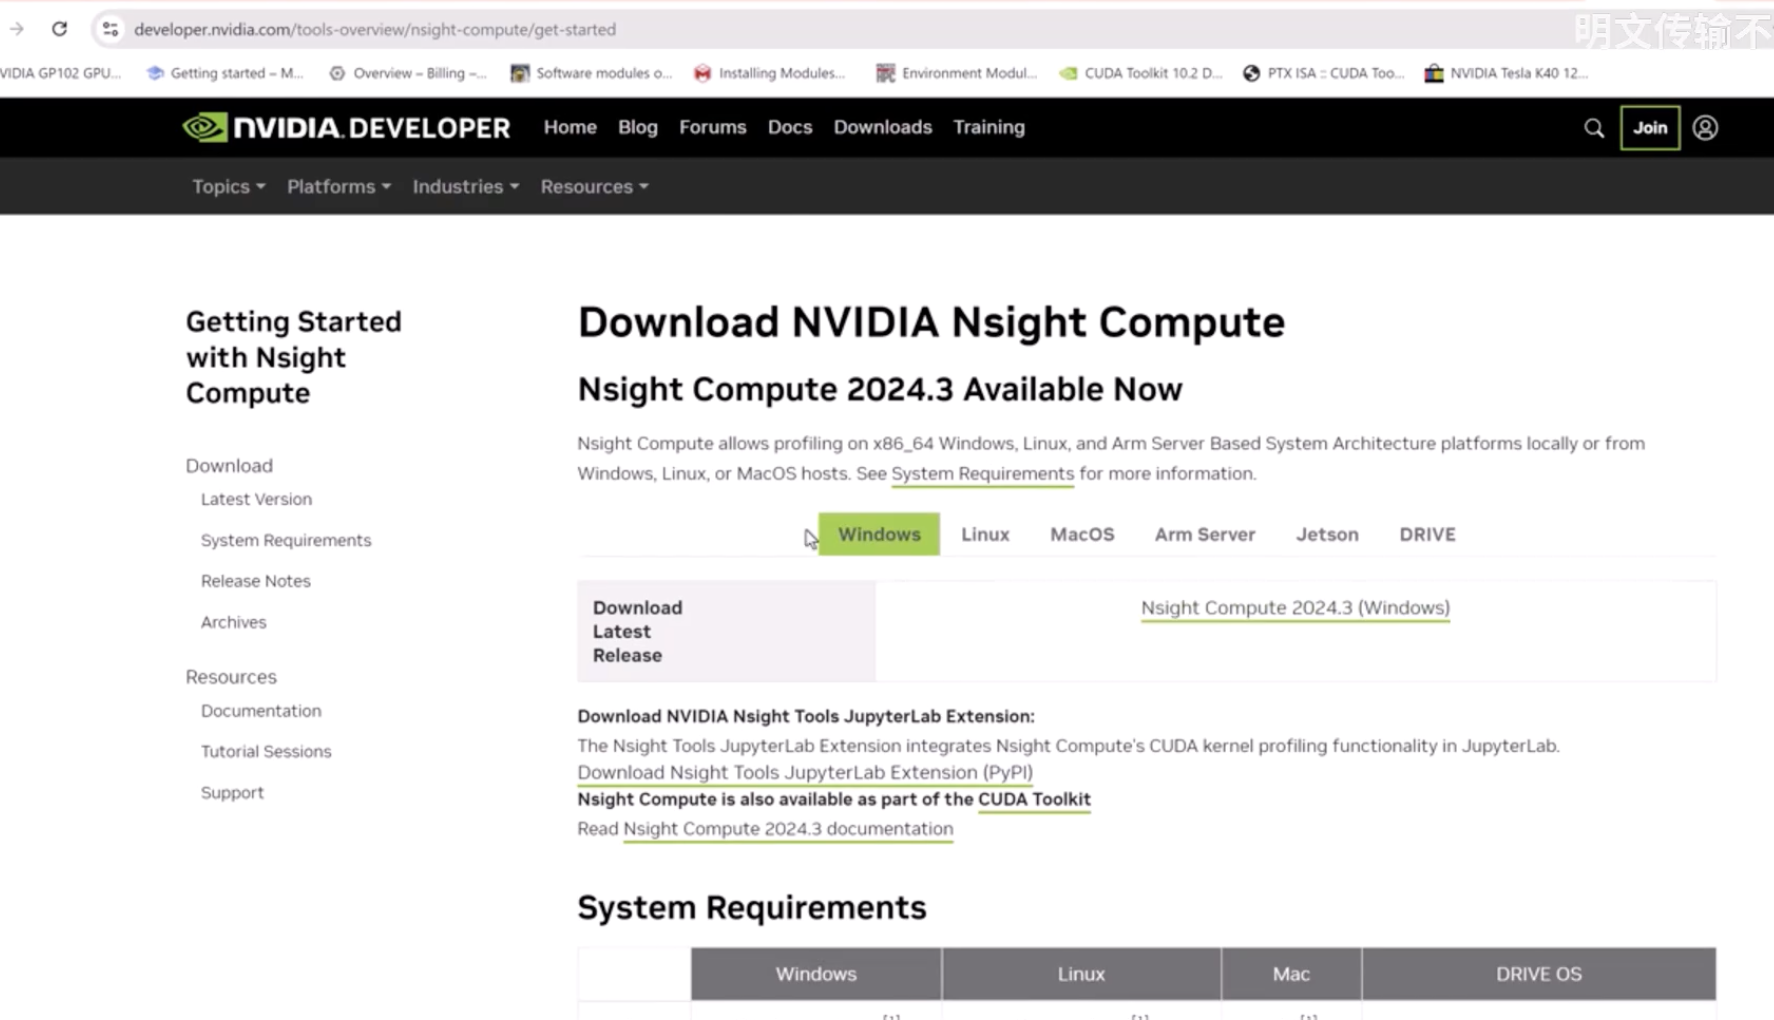
\includegraphics[width=0.75\linewidth]{resources/cuda-105.png}
    \caption{}
    \label{fig:placeholder}
\end{figure}

这里有两个版本，一个是 24.11，第二个是 24.3.2。将打开这个版本。

它是这样启动的，有一些选项，可以打开一个文件、创建一个新项目，或者加载一个已有的项目。这些是 Nsight Compute 图形界面最近的一些增强功能。

需要做的只是从文件菜单打开一个新项目。但在那之前，需要知道 CUDA 应用程序的确切位置。这是 CUDA 课程的文件夹，这是第四节的文件夹。如所示，这里有一些 CUDA 应用程序，还有可执行文件。但在那之前先编译这个 CUDA 应用程序，输入 \texttt{ls}。

有一些 \texttt{.cu} 文件，还有之前章节生成的可执行文件。但今天需要做的是生成带 \texttt{.exe} 扩展名的可执行文件。使用 NVCC 编译器，写例如 \texttt{-o}，这是为了保存编译过程的输出。随便起个名字，例如就叫 \texttt{aa.exe}。

这是可执行文件，这是 CUDA 文件。这个命令会生成这个可执行文件。如所示，这里还没有这个可执行文件。按回车键，然后输入 \texttt{ls}。如所示，这里有了可执行文件。然后回到这里，点击新项目，给它起个名字，点击确定，这里就是配置项。只解释主要的几个。例如这个选项是必须的，这是应用程序可执行文件，已经用这个命令生成了，从这里选择。

复制路径，选择 \texttt{aa.exe} 文件打开。如所示，感叹号被移除了。然后可能需要选择工作目录，例如选择第四节文件夹。

从这里开始有一些配置，比如说是否想启用 CPU 调用栈？是否想启用对 CPU 和 GPU 通信的性能分析过程？如何处理缓存？需要在时钟控制中刷新它们全部。刷新的意思是清除先前存在于缓存中的所有内容。

需要使用基础频率还是无基础？这将指 GPU 的基础时钟频率。对于图分析需要使用节点 1。如果想了解更多，可以从这里查阅文档。

如果现在点击立即启动，它是不会工作的。因为需要开始执行这个应用程序，才能对其进行分析。将添加附加（Attach），可以看到进程名，这里没有任何进程，可以通过这个命令来做到。需要来到这里并开始执行，以便从 CPU 到 GPU 创建一个新进程。

这个命令叫做 \texttt{ncu}。将使用的模式是 \texttt{--launch-mode attach}，然后是 \texttt{./aa.exe}。

那个模式意味着需要让 GPU 开始执行，但它不应该结束。因为需要分析，需要一个正在运行的进程。当按回车键时，例如 \texttt{./aa}，如所示它执行了。但当使用这个命令时，它只是启动了一个进程，消耗了大约 8.2 毫秒。可以通过点击这里的附加来完成。现在可以将这个进程附加到 Nsight Compute UI。

如所示，\texttt{aa.exe} 可以显示在这里，这是进程 ID。先按 Ctrl+C 取消，然后来到这里。

点击附加，再点击这个。需要将参数改为对应的值，因为这是今天的应用程序。点击这个，然后点击附加。现在可以附加了，或者可以来到这里点击启动，如所示一切运行正常。现在需要看看左侧有什么。但它现在是空的，因为还没有开始性能分析。

\begin{figure}
    \centering
    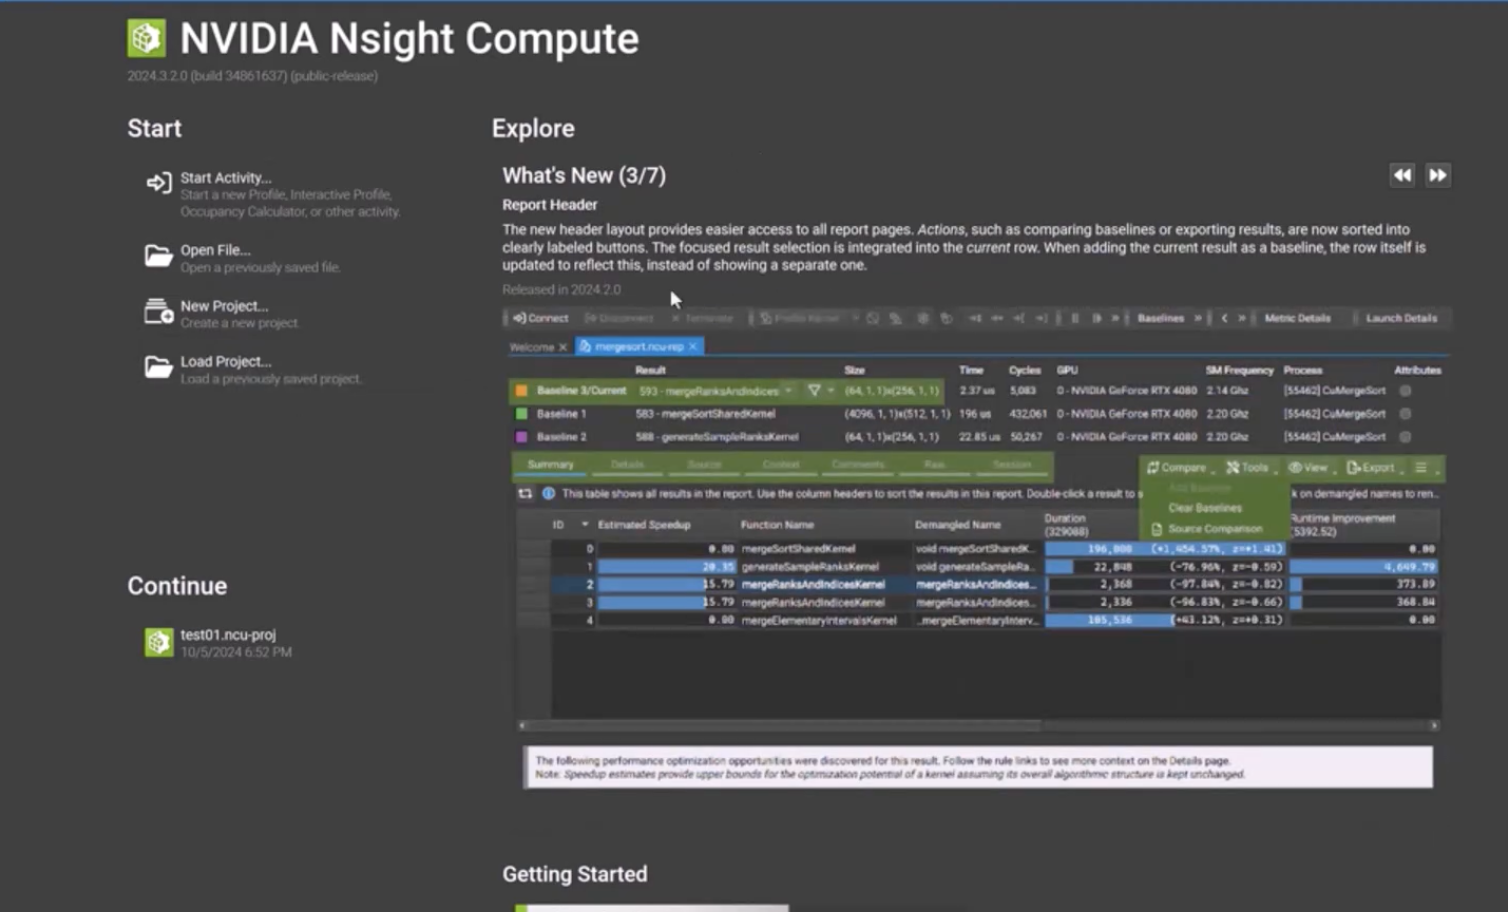
\includegraphics[width=0.75\linewidth]{resources/cuda-106.png}
    \caption{}
    \label{fig:placeholder}
\end{figure}


\subsection{附加进程与指标选择}

在下面的标签页中，可以看到一个叫"指标选择"、"API 统计"的标签页。只是附加到了进程，但还没有开始分析本身。如何开始分析呢？在指标选择中，可以选择任何想要分析的项目，即需要分析哪些指标，需要做哪些性能分析。

从这里开始，选择所有与 Speed of Light 相关的内容，例如 Speed of Light 吞吐量、Speed of Light 屋顶线图（Roofline）、Speed of Light 分层屋顶线图等。如果点击这里，可以看到其他一些选项。同时不选择 PM 采样，但选择计算工作负载（Compute Workload）。如果只想要这些选项中的一个，可以选择它。然后可以在这里选择所有已选的选项，因为它们都非常重要，后面将解释每一个。然后也可以选择指令统计、启动统计、占用率（Occupancy）、GPU 和内存工作负载分布等。

如果还记得之前的讨论，会知道在这里选择的项目在命令行分析中是以部分（Section）的形式呈现的。例如还记得前文中的表格吗？这些就是 Nsight Compute 中包含的部分。

例如看计算工作负载分析，如果来到这里，可以看到计算工作负载分析，然后看一下，例如 Sub-warp 统计。然后再回到这里，会看到 Sub-warp 统计。一旦为分析过程选择了所需的部分和指标，就可以来到这里。同样适用于调度器统计、内存工作负载分析等。然后可以开始点击这里"运行至下一个核函数"。

VectorAdd，这是下一个核函数。选择核函数，然后点击分析核函数，这就是分析过程的开始。一旦点击分析核函数，它将开始执行应用程序，并在执行过程中收集性能指标。

\subsection{分析结果概览}

如所示，分析过程已经完成，可以查看结果了。这里没有结果，因为有很多标签页需要选择。例如有一个摘要（Summary），从这个摘要中可以看到一些信息：已实现的占用率。它解释了理论占用率和已实现占用率。例如理论占用率是 100\%，前文已经讨论过这个了。在命令行分析中的占用率，理论占用率是 100\%，已实现的占用率大约是 80\% 或 81\%。

使用的是相同的指标，但显示指标的方式不同。这里通过一些信息图表来显示，而那里是通过表格来显示的。如果来到这里，可以看到同样的理论 100\%，已实现 81\%。也可以看到这些内容并阅读，但将从另一个标签页阅读。

那个标签页有更多细节，例如详情（Details）标签页，如所示，这里会显示包含的所有部分。例如 GPU Speed of Light 吞吐量，这是第一个；然后有计算工作负载分析；然后是内存工作负载分析。这里有一些技巧可能会给出更多信息，因为可以看到一些表格。

在指标选择中包含的所有内容，都会在详情标签页的这个部分看到其输出。组织得很好。例如可以看到吞吐量，有 16\% 的吞吐量。同样可以再次回到命令行分析，看到这个值也显示在那里。这里只是在两种方法之间建立联系，以便选择最适合的方法。

先看这里，内存吞吐量是 95\%，L1 和 L2 缓存的吞吐量分别是 21\% 和 40\%。在这里可以看到经过的周期数，这个核函数执行的持续时间等。此外如果选择这些选项或指标中的任何一个，可以在这里看到细节。例如，如果在这里选择持续时间，它会显示单位，单位是纳秒，显示值。这里的值是 970，也就是 978，但这里是纳秒，那里是微秒。如果想在命令行分析中做同样的事情，可以使用这个指标。

如所示，\texttt{gpu\_\_time\_duration}。还记得那个分析吗？所有想从图形界面获取、以便于命令行分析一起使用的内容，都可以从这里获取。然后在这个右侧部分的末尾，可以看到 Average、Sum、Minimum。这些在前文中也讨论过。

现在可能会问，为什么最小值、最大值、总和所有这些都有相同的值？因为现在讨论的是持续时间，而对于整个 GPU 的时间，它们应该是相同的。但对于其他情况则不同，例如周期数，每个 SM 使用的字节数就不同。但讨论的是总时间，总时间它们应该相同。

这是第一部分，GPU Speed of Light 吞吐量。然后这里有计算工作负载分析。如所示，有每个周期的指令数（IPC），每个活动周期的指令数，需要搜索它们之间的区别，这是经过的（Elapsed），这是活动的（Active）。这些将在后续章节中讨论。

但这不是本节的重点，因为本节的主要重点是熟悉 Nsight Compute 工具，而不是优化应用程序，也不是理解每个术语。重点是理解 Nsight Compute 工具。在其他章节中将使用 Nsight Compute 工具进行优化。

\begin{figure}
    \centering
    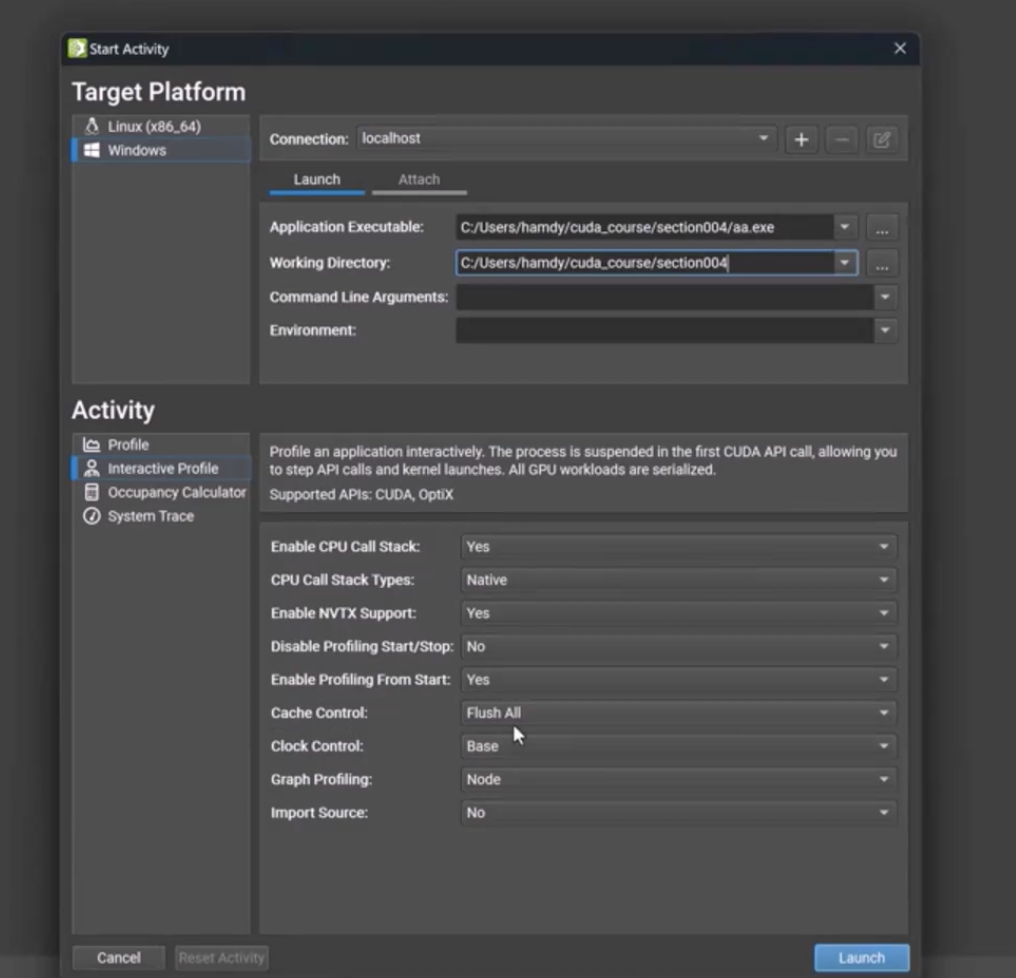
\includegraphics[width=0.75\linewidth]{resources/cuda-107.png}
    \caption{}
    \label{fig:placeholder}
\end{figure}


\subsection{内存瓶颈分析}

接着还有内存工作负载，这里有 SM 繁忙时间的百分比。这里有 L1 的命中率，有 0\% 的命中率。在命令行分析章节中测量过这个，33\% 的命中率，这也非常糟糕。对于 L2 命中率有 33\%，这意味着在内存操作上消耗了太多时间或太多周期。因为必须访问 L1，却找不到需要的数据。然后访问 L2 能找到一些，但其他的数据不在那里。需要从全局内存进行大量读取甚至写入操作，这需要很长时间，需要很多周期，数百个周期。这里只是逐步说明这些数字的含义。

然后有内存繁忙百分比、最大带宽，实现了大约 95\% 的内存带宽。有 95\%，现在可能会想这很好，是个好兆头。但这并不好。因为如果实现了全局内存最大带宽的 95\%，这意味着访问全局内存太频繁了，需要减少这种情况。

理解这些指标的含义非常重要。再看看 L2 缓存中包含了一个叫做压缩的功能，这与 Ampere 架构也有关系。因为这些功能中的一些是从 Ampere 架构开始引入的，而不是之前的架构，比如 Volta、Turing、Pascal 等。然后还有调度器统计，前文已经讨论过调度器统计了。

在讨论 Sub-warp 统计之前，先停在这里。可能会问，这些表格看起来和这里的表格非常相似，简直一模一样。在这里做什么？命令行分析和图形用户界面之间有什么区别？它们显示的是相同的表格吗？但事实并非完全如此。稍后将跳转一下，展示图形用户界面中包含的最佳功能。

这里有 Sub-warp 统计，如所示，有一个非常重要的指标：每个已发布指令的 Sub-warp 周期数。需要阅读所有这些信息。可以说大约需要 119 或 120 个周期来处理每个已发布的指令，这非常重要。需要阅读所有内容，因为这些说明中的一些可以看作是对你的建议或者是一些要点，能帮助优化应用程序以实现高性能。

例如读一下这里的说明："平均而言，这个核函数的每个 Sub-warp 大约花费 111 个周期处于停滞（Stall）状态。"这非常糟糕。停滞意味着这个 Sub-warp 在约 111 个周期内什么都没做。想象一下，有 111 个周期，每个 Sub-warp 就只是停在那里不退出，也不执行任何指令。如果继续看会找到导致这个问题的原因。需要改进这一点，以确保在每个周期内尽可能让每个 Sub-warp 执行一些操作，执行一条指令。

这背后的原因是什么？说过有 111 个周期的停滞。"等待长计分板依赖（Long Scoreboard Dependency）"，可以阅读来了解，这里的依赖意味着某个指令正在等待前一个结果或从内存的读取操作。它说明依赖是由于从 L1/纹理缓存读取数据，或者可能是来自其他内存层级。例如本地内存、全局内存、表面内存或纹理操作单元。可以从这里知道遇到了内存瓶颈问题。

\begin{figure}
    \centering
    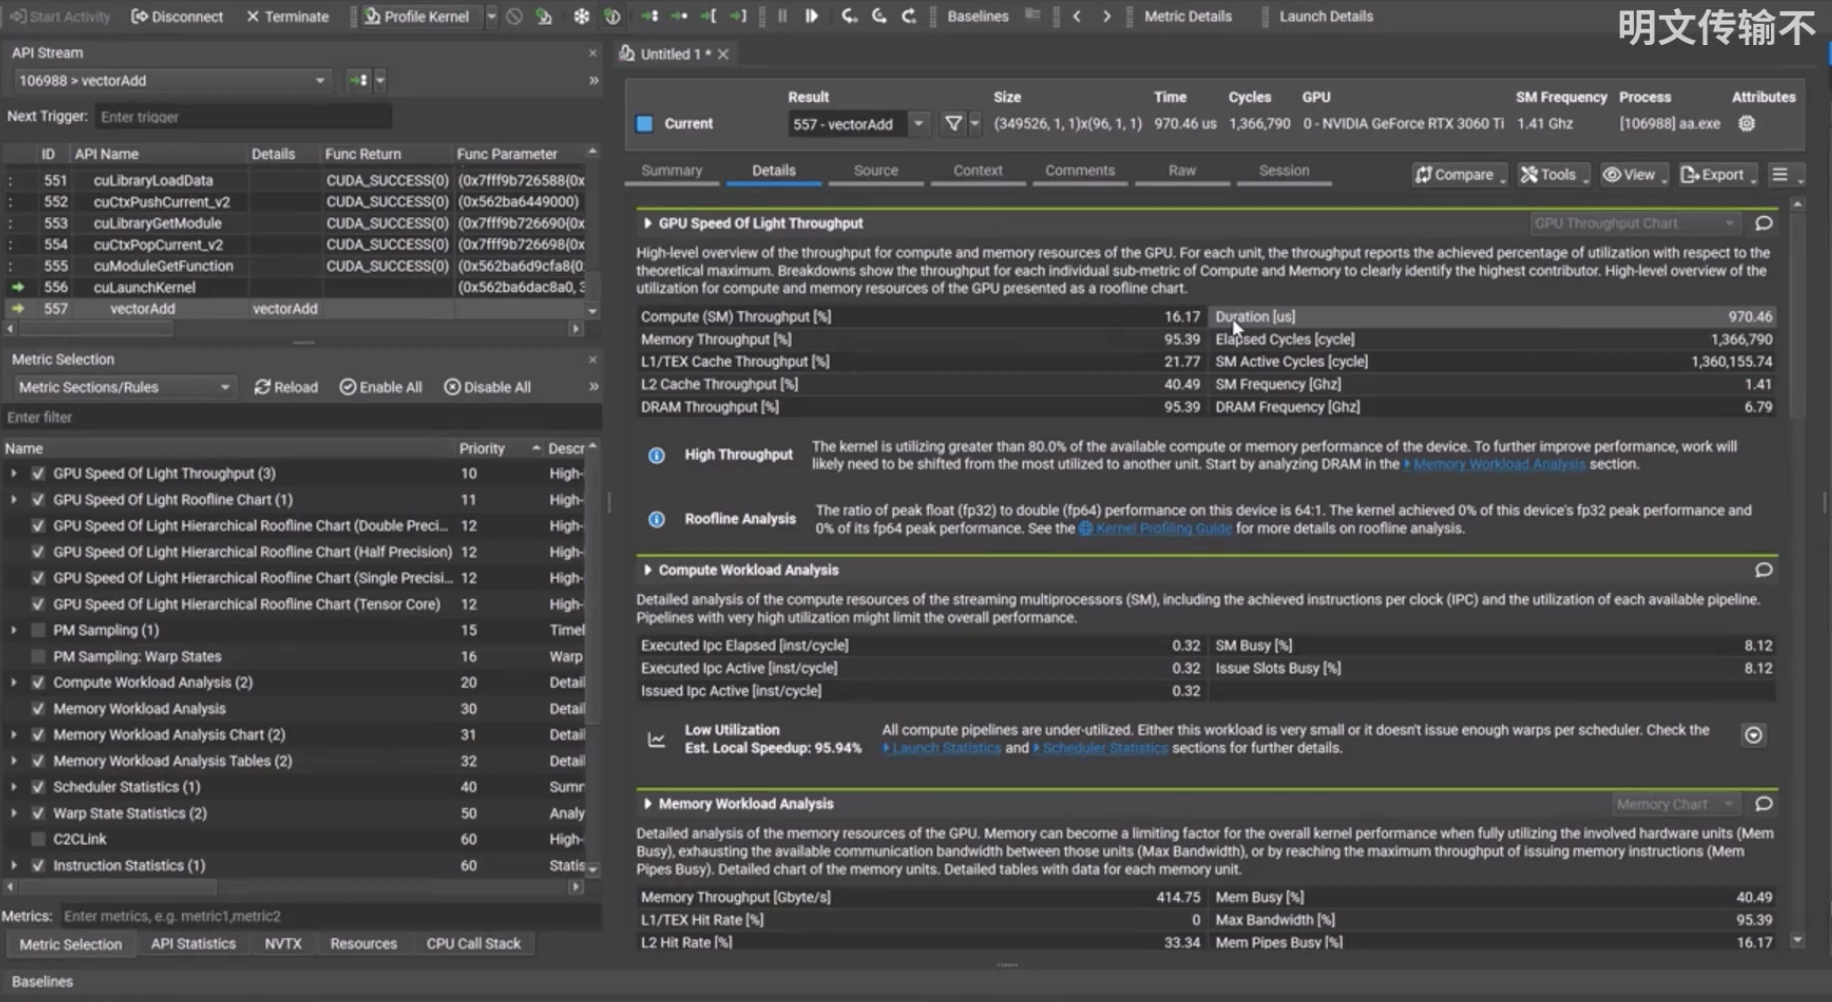
\includegraphics[width=0.75\linewidth]{resources/cuda-108.png}
    \caption{}
    \label{fig:placeholder}
\end{figure}

\subsection{源代码与汇编分析}

回到这里，还记得最大带宽吗？当说如果正在实现一个高带宽时，高内存带宽在某些情况下可能是好的，但在其他情况下就非常糟糕。这就是这些指标与在 Sub-warp 统计中看到的停滞是如何关联的。特别是当 L1 和 L2 命中率很低时。然后可以看到每个 Sub-warp 有 32 个线程，每个 Sub-warp 有 30 个未被屏蔽（Unmasked）的线程。

继续看查找产生数据的指令。但在那之前来到这里，点击视图标签页，然后点击这里的展开所有部分。它说需要找到导致停滞的指令，下面展示这一点。如所示，这就是图形用户界面和命令行分析之间的主要区别。这是添加到 Nsight Compute 图形界面中的最佳功能。看到这个部分了吗？如所示，拥有相同的部分。除了图表之外，这里没有添加任何新内容。

看到计算工作负载了吗？看到内存工作负载了吗？可以很容易地阅读它，但添加了一些图表，以便用一种好的方式将数据或分析输出可视化。

例如，这里有两个重要的吞吐量或利用率计算：SM 吞吐量和内存吞吐量。说过内存吞吐量是 95\%。但计算吞吐量是多少呢？16\%，这意味着这个应用程序是内存瓶颈型（Memory Bound）的，为什么？因为它只使用了 16\% 的算术逻辑单元（ALU）。只利用了 16\%，但从内存方面利用了 95\%。

这意味着应用程序大部分时间在进行内存操作，而不是算术运算。不需要这样，需要在提高 L1 和 L2 命中率的同时，稍微降低这个数值。因为如果提高了 L1 和 L2 的命中率，那将减少内存带宽的使用。同时增加算术运算，以充分利用可用的硬件核心。这就是如何解释内存瓶颈或者说应用程序的瓶颈——它是计算瓶颈型（Compute Bound）还是内存瓶颈型。

这是第一个图表，非常重要。也可以阅读这两条说明，因为可能会给出一些启发。也可以点击这些链接，一些是在线的。如果点击这里，这将带你到内存工作负载分析部分。

看看计算工作负载分析。如所示，这只是对不同类型算术操作及其利用率的可视化呈现。例如这里有 FMA 单元或 FMA 指令。FMA 指的是融合乘加运算（Fused Multiply-Add），而 ALU 则包含除双精度外的所有其他算术操作。这将包括例如单精度、半精度、整数精度等。这里使用了大约 3.55\% 的可用资源用于融合乘加运算。

而这里使用了大约 4\% 左右，但这指的是活动周期中的百分比，意思是如果整个 GPU 有 100 万个活动周期，大约使用了其中的 4\% 来执行 ALU 运算。另外 4\% 或 3.55\% 用来执行乘加运算。

后面将给出一个关于这个的实际例子。这里有其他单元，例如加载/存储单元（LSU）。不确定 IDU 指的是什么，但双精度在这里。无论如何，这是相对于执行的峰值指令数而言的。意思是从白皮书中知道，在这款 GPU 这个架构上，不同类型的算术操作有一个可执行数量的峰值。假设例如加载/存储单元的峰值是 1000 TOPS。这里只使用了峰值数的 16\%。可以看到这里执行了太多的加载和存储单元指令。

加载和存储单元执行什么操作？内存操作、全局内存、L1/L2 内存操作或者共享内存操作。如果把它与 ALU 和 FMA 相比，这并不好。可以看到，这个单元的待执行指令数量很大。而这是因为如果内存操作相比 ALU 来说很大，这将导致内存瓶颈。

看看内存工作负载分析，这非常重要。因为它会给出一个概念，并提供更多关于有多少请求、在不同内存层级之间移动了多少数据等细节。这里没有使用任何单精度或双精度，这就是为什么它们都是零。

这里有主要的内存单元，例如有共享内存加载、全局内存存储、共享内存。这是稍后会讨论的单元，先别关注它。另一个单元叫做表面内存、纹理内存、本地内存和全局内存。这是第一级，这里有它们的第一级。还记得命令行分析吗？\texttt{l1tex\_\_...}，这是 L1 缓存。还记得这些指标以及它们是怎么写的吗？如所示，它们显示命中率是 0\%。

从这个图形界面可以读取许多性能指标，而无需费力去阅读指标名称、硬件单元名。需要提醒一下，看到这个了吗？有十万个指标，还记得吗？

这里一切都组织得很好。这比试图搜索需要知道的指标在哪里、描述是什么等要好得多。如所示，L1 缓存的命中率是 0\%。对于共享内存没有请求。因为在这个应用程序中，如果没有使用共享内存，只是在不使用任何共享内存的情况下将两个向量相加。这就是为什么这里的请求数量是 0。

然后是第二级 L2 缓存，这里是零或者说是 33\%。如所示，在它们之间有传输的数据量，可以计算所有这些。然后从 L1 到 L2，这意味着写入结果，因为正在读取向量 A 例如从 L2 到 L1，移动了大约 268 兆字节和向量 B，然后计算单元将完成执行，写入的数据量大约是此值的一半。因为读取两个向量，但只写入一个向量即 C 向量。然后 L2 缓存中的命中率是 33\%。

接下来给你一个任务，需要搜索如何提高 L2 缓存的命中率。只是思考一下，看看是否能做些什么。然后这是设备内存，也就是最后一级。有全局内存、L2 缓存、L1 缓存以及计算单元本身之间的请求数量。这来自 ALU，来自 SM。而内存单元会将这些操作发送到 L1 级。大约有 315 万条指令从 SM 发出，到达加载和存储单元或全局内存操作单元。

然后 L1 级如果没有命中，会将这些请求发送到 L2。L2 如果命中，它会将结果或数据发送回这里。如果没有命中，它将向设备内存请求这个数据。这里展示的就是这个情况。这就是内存图表图形界面的样子。大约有 100 万次请求从 SM 发往 L1，大约有 210 万次对这些请求的回复。

如所示，不太确定具体如何解读。这里说例如如果看到这个颜色，这意味着正在达到峰值。例如看这里，如果记得设备内存的吞吐量是 95\%，可以看这里，用了这个颜色。因为有 95\%，但对于 L2 有 33\%。

这就是为什么它在这个区域是这个颜色。对于 L1 有 0\%，它是深色的。如所示，这是一个非常重要的图表。然后这里有调度器统计。再次建议阅读这里的所有内容，GPU 每个调度器最大 Warp 数，如果记得应该是 16。

在这个应用程序中实现了 12 个，有一个不错的值。如果有 16 个，而实现了 12 个，这很好。这是每个调度器的理论值，数值也是 12。每个调度器的活动 Warp 数大约是 9.69，这是理论的，这是实际达到的。然后每个调度器的合格（Eligible）Warp 数和每个调度器已发出的 Warp 数。总之现在不关注所有这些，这里相同的数据用图表可视化了。

如所示长时间计分板停滞（Long Scoreboard Stall），大约是 111 个周期停止等待。可以查看这个 Warp 采样。搜索一下长时间计分板停滞。但不管怎样，这里有短时间计分板停滞（Short Scoreboard Stall）。

这是指如果命中了某个内存层级，但这是指如果计算所有层级的平均值。然后有指令统计。这与不同的指令有关，停滞、耗尽（Throttle）、选定存储屏障。需要查找更多关于这些类型停滞的信息。例如整数乘加指令，意思是所有这些指令都在这个应用程序中执行了。并且获取每一条汇编指令，试图告诉你每条指令在应用程序中执行了多少次。

例如看乘加指令，可以看到它执行了超过 400 万次。\texttt{S2R} 这是用来读取时钟之类的，大约是二百多万次。有一个从内存加载值的加载指令，如所示，它也执行了超过 200 万次。移动指令超过 200 万次，退出指令等。还有将两个值相加的 \texttt{IADD} 指令，执行了一百多万次。

如果想查看这个应用程序中的所有指令，可以转到源代码（Source），这是这个应用程序核函数的汇编语言。这是汇编语言，这是 CUDA 的代码。这是这个核函数的汇编语言。还记得这里的内容吗？

需要加载 A 值，然后加载 B 值，将它们相加并将结果存储在 C 中。这里读取线程 ID、块 ID 并进行一些计算，比如加法和乘法，并将值存储在 i 中。这里使用 i 值从内存加载 B、从内存加载 A、将两个值相加，并将结果存储在 C 中。这就是将在汇编语言输出中看到的内容。

例如看看这个，还记得这个指令吗？这只是读取一个寄存器，一个预定义的寄存器，如所示这个值线程 ID，这个值 CTID，前文中说过 CTA 指的是块 ID。一旦读取了线程 ID 和块 ID，如果还记得这里，需要进行加法和乘法。这就是为什么这里有 \texttt{IMAD}。\texttt{IMAD} 指令将在这里执行，这里还有另一个 \texttt{IMAD}。一旦通过 \texttt{IMAD} 计算完所有这些值，需要将它们存储在这个值即 R6 值中，这就是 i 变量。然后有 \texttt{EXIT}，因为 if 语句的条件没有满足，那么需要退出。

如果 i 不小于 N 需要退出核函数，然后需要执行 if 语句。这就是在汇编语言中做 if 语句的方式。但如果不是，如果 i 小于 N 需要执行这个，这就是为什么这里有 \texttt{EXIT} 指令。如果达到了语句的条件，意思是需要执行这里的这个命令，那么将执行 if 语句内部的内容。

如所示，不会看所有的指令。但这里是前几条指令，前四条指令只是获取 i 值。需要在这里做的是有一个加载 A 的指令，一个加载 B 的指令。这是从内存加载，这也是从内存加载，然后需要乘加。因为一旦加载了 B 和 A 需要将两个值相加。这就是为什么需要 \texttt{IMAD} 或 \texttt{ADD} 指令。

\begin{figure}
    \centering
    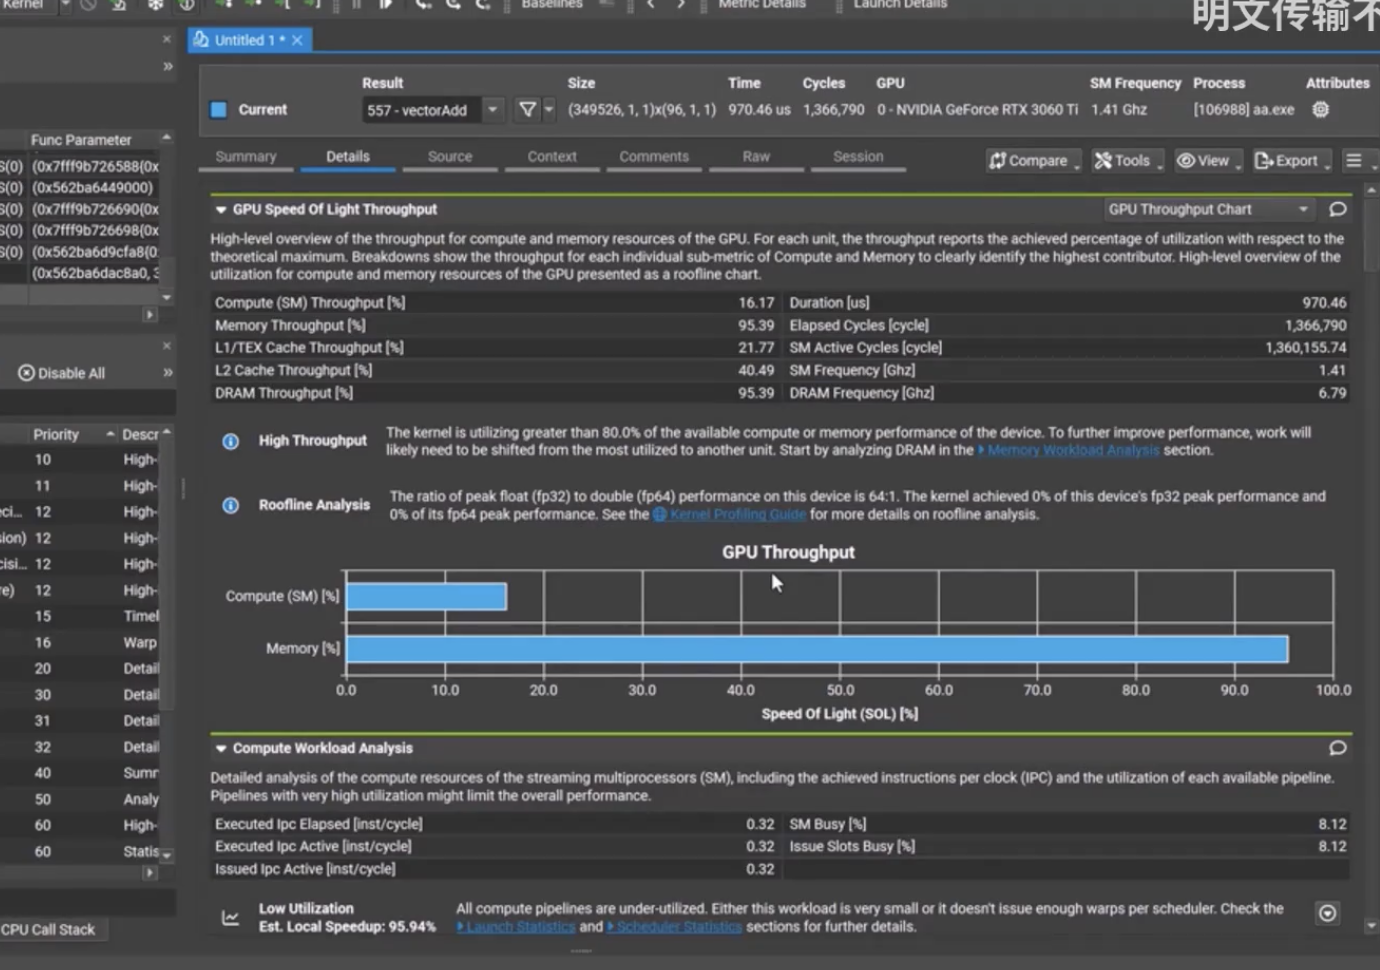
\includegraphics[width=0.75\linewidth]{resources/cuda-109.png}
    \caption{}
    \label{fig:placeholder}
\end{figure}

\subsection{指令依赖与停滞分析}

现在不解释为什么这里两者都有。R4、R3。但想象一下可以把 \texttt{IMAD} 当做 \texttt{ADD} 使用，然后还有 \texttt{ADD}，这是加法过程。读取 B 值并存储在 R3，因为读取 A 值并存储在 R4，然后如所示，在这里将 R4 和 R3 相加，并将值存储在 R9。但不管怎样，现在不想关注这个命令。但能看到这里的感叹号吗？如所示，如果把鼠标移到这里，会看到这个信息。这一行指令要对 84\% 的停滞负责，所有 Sub-warp 停滞的 84\%。

再看一下这一行指令停滞的 99.7\%，这一行指令导致了停滞。可能会问为什么是这一行？这只是加法，为什么加法过程会导致大量停滞？

如所示，有一个依赖，如果不从内存读取两个值，就无法对它们进行加法。这个加法将等待直到从内存获取 R4 和 R3。这就是为什么这里有依赖，这个依赖可以在这里显示出来。确认一下，有这个信息。

是的，如果引用这个指令，这些就是对依赖的解释。这个依赖于这个和这个。每当在这里看到这个，这意味着这个依赖于前面的那个。看看这个指令依赖什么。如果到这里看看这个三角形符号，从汇编代码看，它应该依赖于 R3 和 R4。这是三角形符号。它具体在哪里？是的，这里有一个依赖。

看看这个，看到 R4 了吗？如所示，依赖于 R4。但也应该看到，这里有什么依赖于 R3。

集中在这里，R4 在这里和这里都存在，这个指令需要等待来自这里的 R4，然后这个指令需要等待来自这里的 R4，情况就是这样。还有看看这个，每当看到右侧的这个部分，就会看到依赖关系。例如再次集中注意力，这里有一个向右的箭头，如果向上看会发现它依赖于 R4。这里同样这个指令有另一个向右的三角形。R3 也有一个向右的三角形，它依赖于这里的这个指令。如果点击这里，会发现它也依赖于 R3。如所示 R3，这就是这里展示的依赖关系。

回到这里查看已执行的指令，这是每条指令执行时间的百分比。但可以看看这里的 Warp 停滞采样，可以看到这个指令导致了大约 93\% 的 Sub-warp 停滞。因为它等待前面所有指令的结果，而前面所有指令又依赖于更前面的指令，这是最后一条指令，它依赖于前面的所有指令。

同样对于存储指令，也是因为一旦完成了加法过程或加法操作，需要将值存储到内存中的 C 里。这就是为什么这里有一条存储指令，\texttt{STG} 存储到全局内存。需要从加法过程或加法操作中取出 R9，并将其存储在 C 值中。如所示，同样这条指令导致了 93\% 的停滞。这解释了这里的一切。在 Sub-warp 统计中，看看有什么。

是的，从这些选项中可以确定其他一些选项。例如有地址空间，可以从这里开始查看已执行的指令，但可以专注于地址空间。地址空间意思是在这里访问的是全局内存，但可以左右移动这个来查看所有内容，这也适用于全局内存。如果看这条指令，正在从全局内存加载，这些信息非常重要。

这是加载不是存储，但这里是存储。而扇区（Sector）是一个扇区，这里的扇区大小是 32 字节。因为如果还记得前文，一个扇区等于 32 字节。很多线程不仅仅是相加两个元素，每个是四字节加四字节，正是相加两个元素。但是是针对不同的线程，所以每个线程将需要四字节，这就是为什么每次指令执行加载 32 字节。

是的，这是寄存器的活跃性。还有其他内容吗？不确定活跃寄存器的含义，但可以稍后讨论。如果有其他核函数，可以从这里选择核函数。这里是 SASS，但没有生成 PTX，所以关注的是 SASS 指令，现在先跳过它。上下文，这是稍后需要讨论的内容。

环境（Environment），在这里可能会看到一些关于操作系统的信息。比如 Windows 11 名称、创建时间，拥有的 CPU 主机架构等。如果想查看这些信息，这只是其中一部分。如果 Nsight Compute 图形界面提供了关于性能分析的注释，这里应该包含一些注释，但不需要看这个。

回到详情，看看是否还有其他需要查看的东西。这里有一些说明，如果增加每个线程的寄存器数量会发生什么？实现了大约超过 40\%，好像是 50\% 左右。在纵轴上有 Sub-warp 占用率。这里这个 48\%，这是因为每个线程使用了 16 个寄存器。但它说如果改变应用程序代码来增加每个线程的寄存器数量，将会降低 Sub-warp 占用率，正如这个图所示。这意味着可以从这个图中了解到，可以将每个线程的寄存器数量从 16 增加到 40，而不会导致 Sub-warp 占用率的下降。

这就是需要从这里学习的。可以将每个线程的寄存器数量从 16 增加到 40，而不会导致任何下降或损害 Sub-warp 占用率，这对性能来说是非常重要的。如果将每个线程的寄存器数量增加到超过 40，那么将会导致性能问题。同样适用于块大小——应用程序性能。它说在这里，在这个点上块大小是每个块 96 个线程，使用每个块 96 个线程，可以从这里的启动统计中看到这一点。它说，如果将这个数字从 96 增加到 128，Sub-warp 占用率将不会有任何影响。

这里只讨论 Sub-warp 占用率，但如果到这里将其增加到例如 800，将大大降低占用率，从 48\% 降到大约 24\%，相当于占用率下降了 50\% 左右。但如果例如将其增加到 224，将稍微降低占用率。如果降低了占用率，将会影响应用程序的整体性能。如果增加了使用的共享内存，将会导致占用率的下降。同样适用于每个块的共享内存，但这里是因为在这个应用程序中没有使用共享内存。

不打算再次解释所有这些，但需要看看这部分。这是总数，不是每个 SM。在解释 Warp 停滞采样，并说有 47000 次停滞。它说可以点击这里来了解是哪条指令导致了所有这些停滞。如果还记得从源代码标签页，知道这条指令导致了大部分的停滞。但可以点击这里，它会带我们到同一条指令。

可以从这里的百分比值看到停滞的第二大原因。不知道是否有更多，但可以来到这里点击导致停滞的第二条指令，它会带我们到那个分支。再次点击这里，它选择了这里的这个，因为这个导致了 2\% 的停滞。无论如何，这是针对执行最多的指令。如果点击这里，它会带你去那条执行了一百多万次的指令。点击这里，这条执行了一百多万次，可以对其他的做同样操作，但不全部演示。

\subsection{占用率计算器与优化}

\begin{figure}
    \centering
    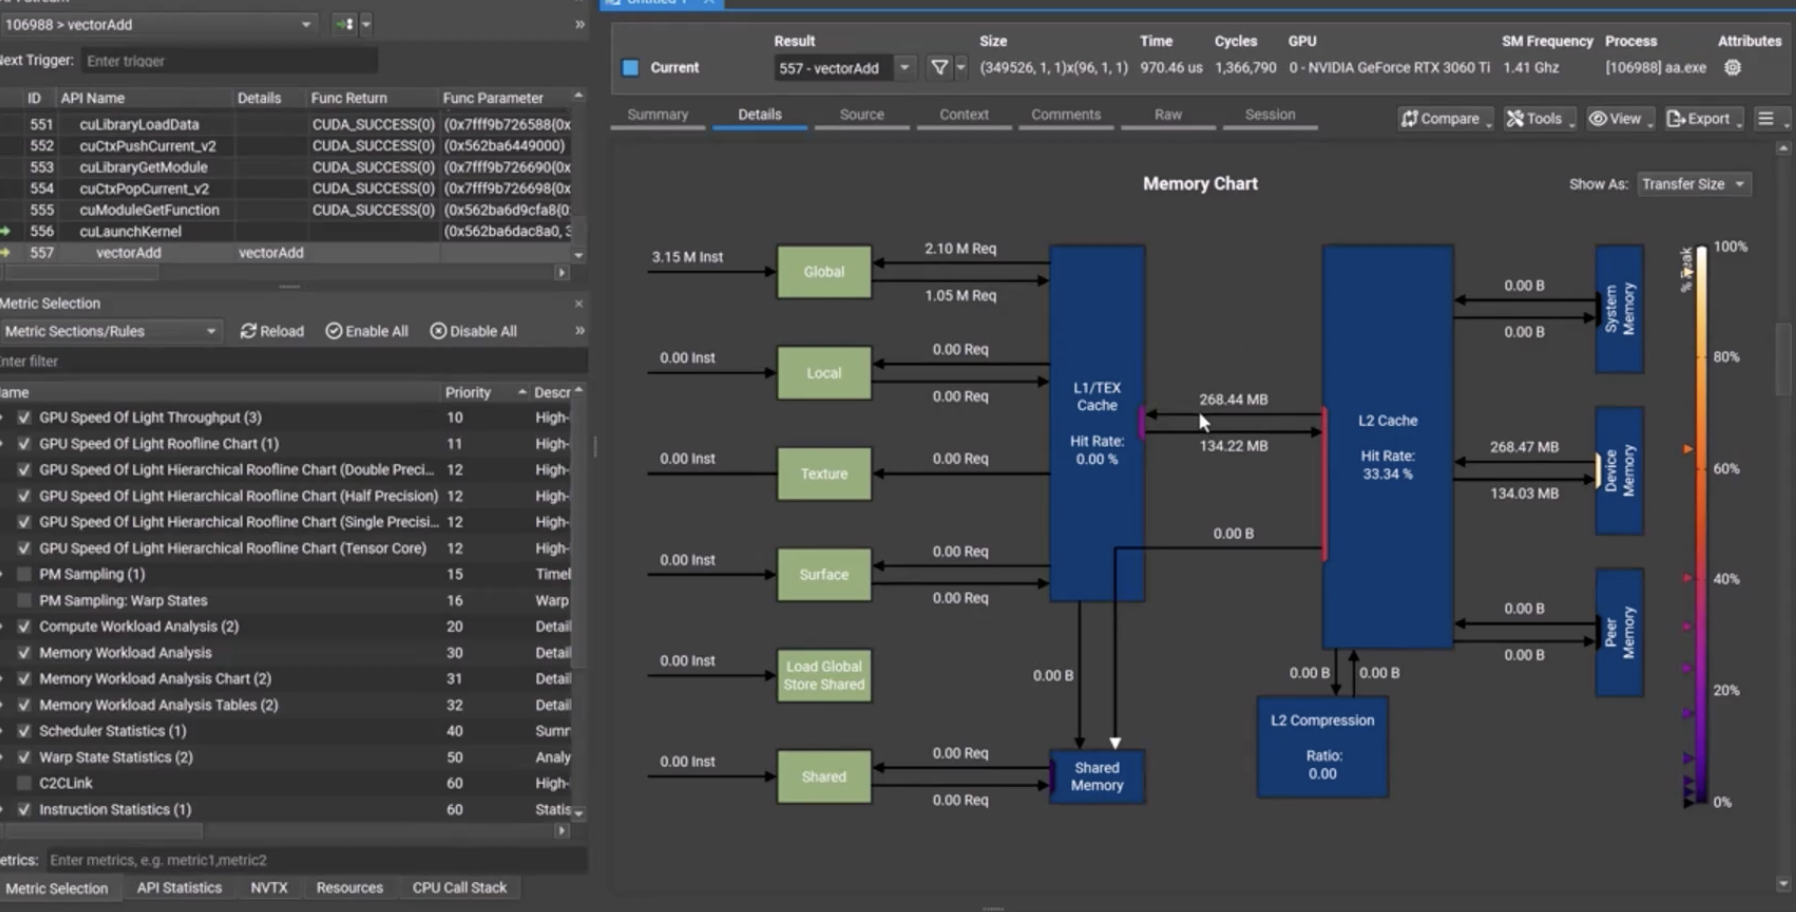
\includegraphics[width=0.75\linewidth]{resources/cuda-110.png}
    \caption{}
    \label{fig:placeholder}
\end{figure}

\begin{figure}
    \centering
    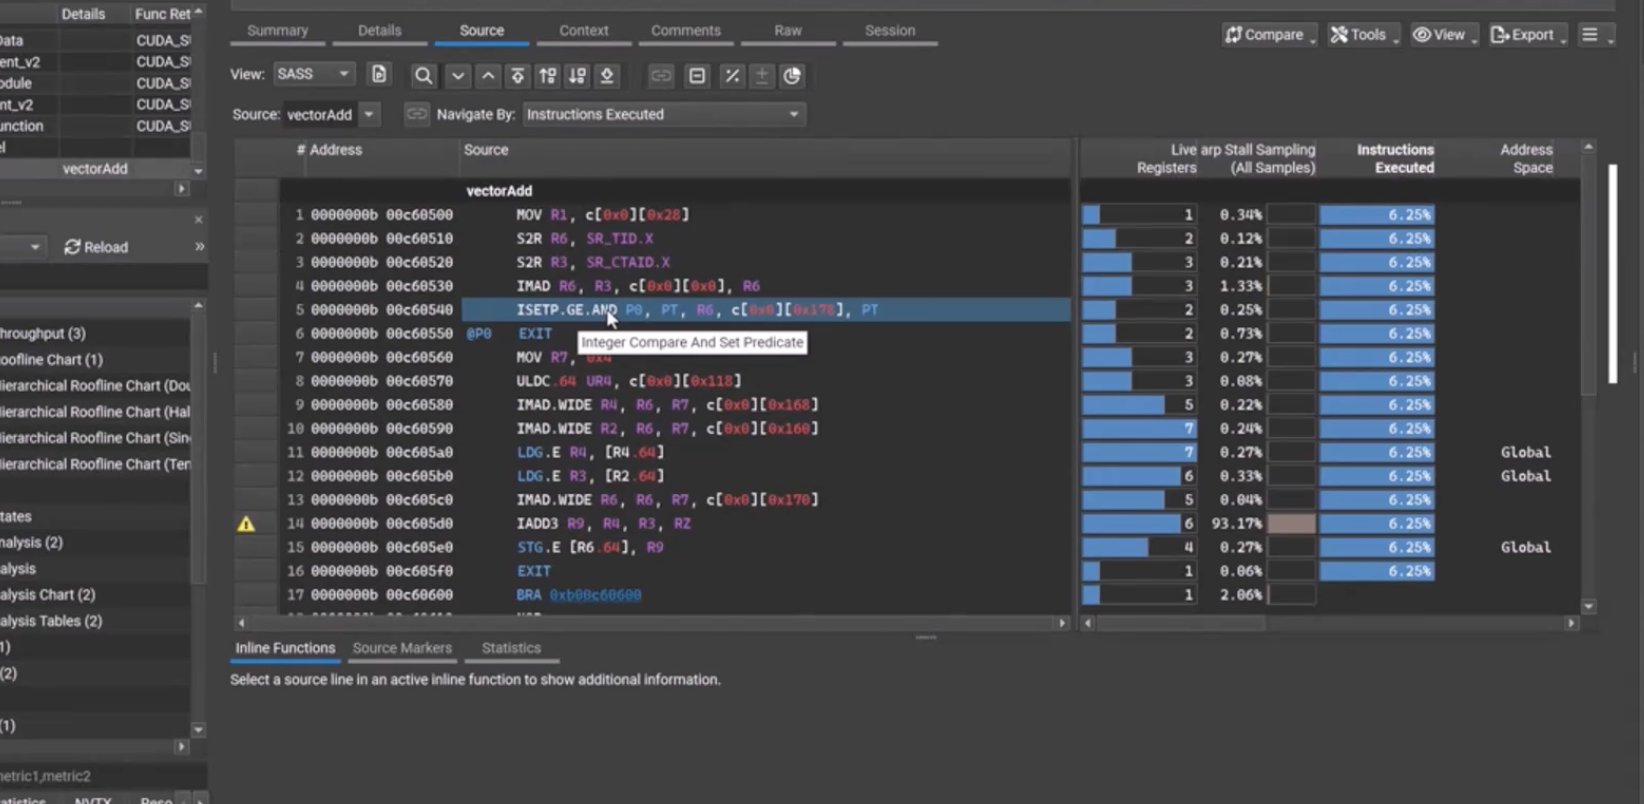
\includegraphics[width=0.75\linewidth]{resources/cuda-111.png}
    \caption{}
    \label{fig:placeholder}
\end{figure}


\begin{figure}
    \centering
    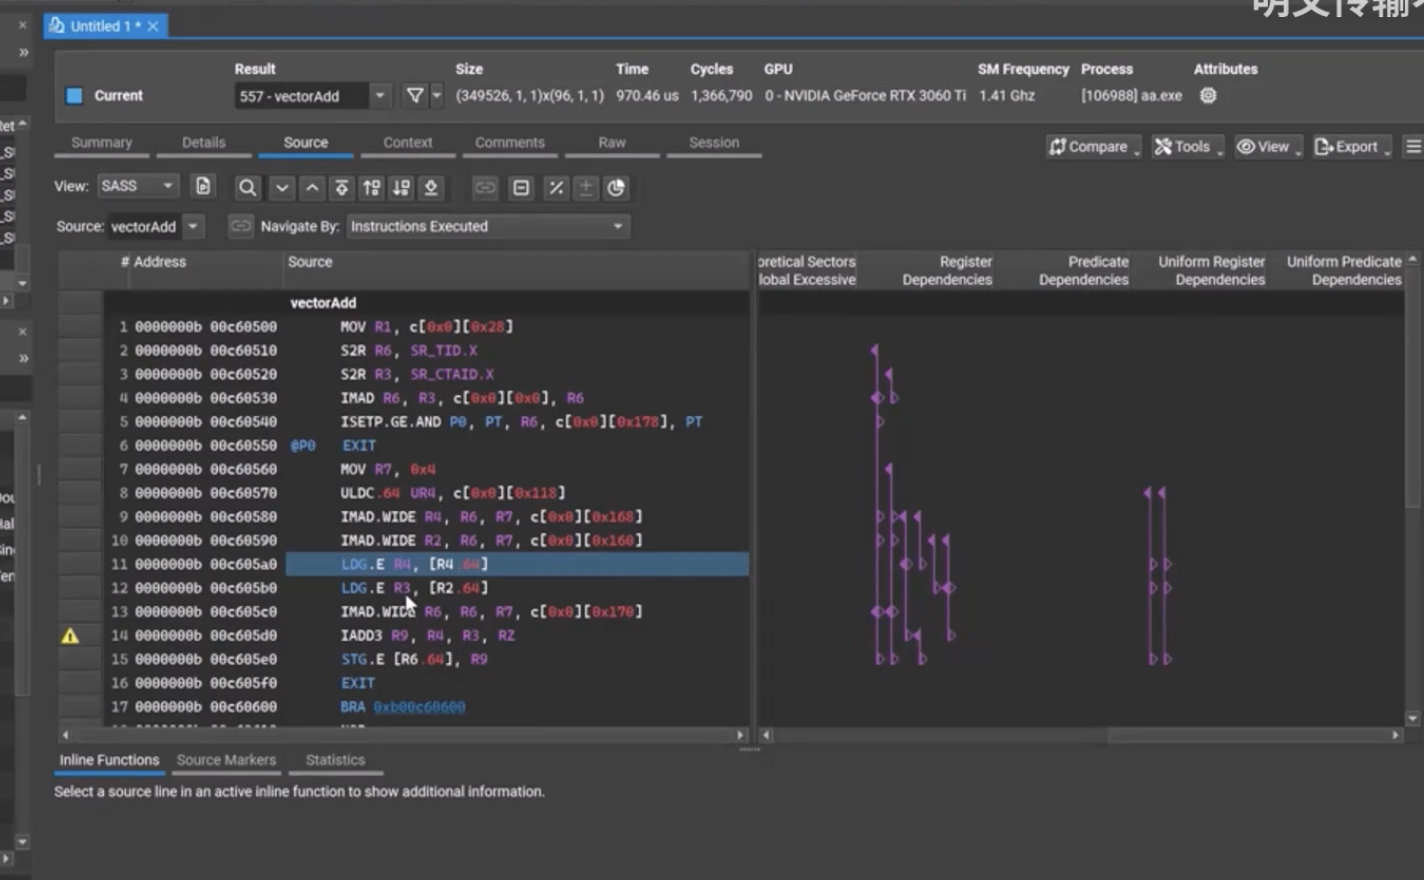
\includegraphics[width=0.75\linewidth]{resources/cuda-112.png}
    \caption{}
    \label{fig:placeholder}
\end{figure}


\begin{figure}
    \centering
    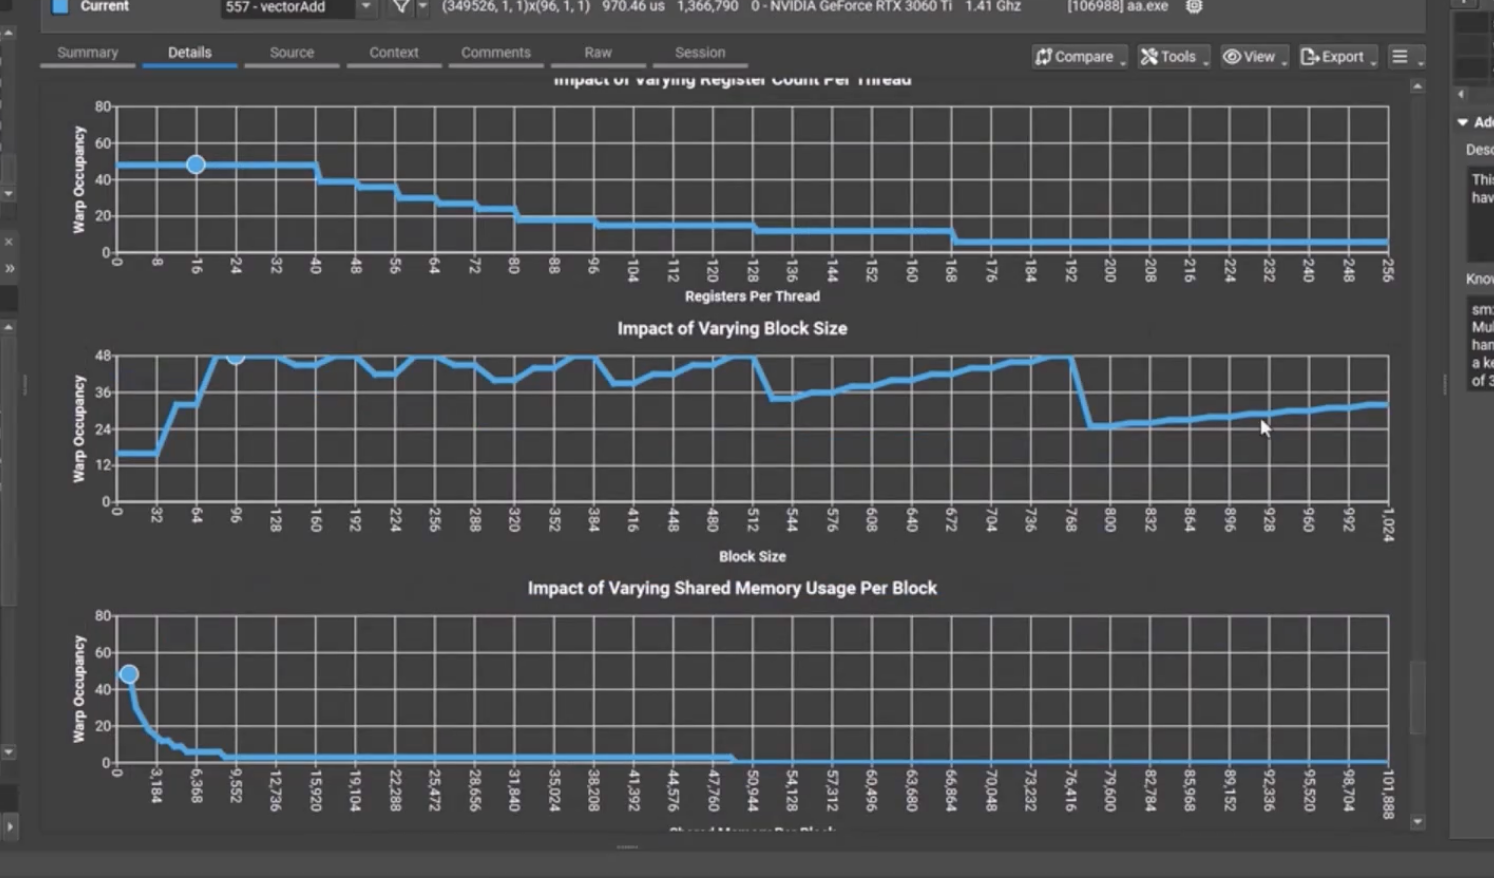
\includegraphics[width=0.75\linewidth]{resources/cuda-113.png}
    \caption{}
    \label{fig:placeholder}
\end{figure}


这就是 Nsight Compute 用户界面的工作方式。关于它就是这样了，只是确认没有其他内容了。是的，这里指标详情这个标签页，当点击这里并点击这里，这会显示任何所选项目的详情。当选择某个项目时，它会把详情显示在这里，然后也可以显示占用率计算器（Occupancy Calculator）。前文讨论过这个计算器以及如何计算占用率。可以在这里修改这些数字，看看它们对占用率的影响。

同样前文在另一个标签页看到的这些图表在这里也有解释，但在这里可以操作它们。可以在这里修改并观察对数值的影响。不确定现在是否有效。是的，它起作用了。比如说 1024，比如说如果点击这里的 256，看到了吗？看到变化了吗？

这也是一个很好的功能，可以看到这些配置对性能的影响。可以折叠各个部分以隐藏图表，只看数字。还有什么功能？然后可以把性能输出在这里，导出或保存为 PDF、图像或其他格式。

可以设定一个基线（Baseline）。如果有一个核函数并想将其与其他核函数进行比较，可以在这里进行比较。可以将一个核函数设定为基线。还能在这里查看什么？从这里开始有一个叫做 API 统计的功能，可以查看或者说隐藏这里的任何部分。从这里这将展示 CUDA 的运行时 API。还记得吗？前文有关于运行时 API 的章节，所以需要看那个章节来理解这里讨论的内容。

\texttt{cudaMemcpy} 操作，这被称为 CUDA 运行时 API。\texttt{cudaMalloc} 在 GPU 的全局内存中分配空间，这也被称为 CUDA 运行时 API。同样适用于在应用程序中使用的所有其他函数，但这非常重要，因为它解释了这些 API 在这个应用程序中各消耗了多少时间。例如仅仅将数据从 CPU 复制到 GPU 或反之，这就消耗了大约 40 毫秒。在 GPU 中分配空间，这大约需要 7 毫秒。同样这与核函数执行无关。这里只是将数据从 CPU 复制到 GPU，而这里再进行分配。还记得这里的指针吗？这显示了曾经执行需要的时间。大约是 7 毫秒，这些 API 需要多少时间？可以看看这些 API 各需要多少时间来执行。

不需要看所有这些东西，只需要关注指标选择和 API 统计。据所知，还可以从这里选择许多其他选项，例如这个显示或隐藏这里的内容。可能需要做的事情之一是，例如添加另一个选择项。这个分析如果想要分析核函数，比如说修改了核函数中的任何内容并想再次分析它，只需点击这里或这里。如果添加了另一个选择项，需要从这里再次分析核函数。

然后从工具菜单有项目资源管理器、输出消息。看看输出消息，没有任何输出消息，也可以看看这里的选项，可以查看诸如字体等选项，这是针对用户界面本身的，可以选择一些配置，轻松地操作这些设置。然后从窗口菜单，可以显示或隐藏这里的一些窗口。

这就是关于 Nsight Compute 工具的图形用户界面的全部内容。但这并不是使用 Nsight Compute 工具的结束。因为当开始讲解性能章节和优化时，将基于从 Nsight Compute 获得的结果进行优化。


\section{性能分析方法论}

本章将对上一节最后一个应用程序进行一些性能分析。需要做的只是改变块大小（Block Size），看看它如何影响不同的性能指标。从 CUDA 代码开始，如所示，这里有一个将两个向量相加并将结果存储在第三个向量中的核函数，该向量称为 C 向量。然后在主函数中，遵循一般 CUDA 应用程序的步骤。如所示，定义了一些指针，然后在 GPU 中为这些向量或指针分配空间，然后在 CPU 端做同样的事情，并初始化向量 A 和 B，然后将数据从 CPU 中的 A 和 B 复制到 GPU 中的 A 和 B，以便能够在 GPU 中执行加法操作。然后执行核函数来执行加法操作，最后使用 \texttt{cudaMemcpy} API 返回结果。这就是在这个应用程序中需要做的和需要了解的全部内容。

这里需要控制或操作的是每个网格的块大小变量。实际上有两个变量，不是一个。因为如果还记得，对于任何 CUDA 核函数，有两个配置。第一个是每个块的线程数，第二个是应用程序中的块数。如果搜索这个，可以往上翻，看到正在从终端读取这个值。当执行这个应用程序时，需要在执行时添加块大小，并且这个值将被输入到这里的这条指令中。相比于上一节讨论的内容，这只是在应用程序中所做的唯一更改。

回到这里，这个文件叫 \texttt{test\_01}。这里有一个名为 Section 05 的新章节，输入 \texttt{ls} 命令，这是文件。需要编译这个文件，写 \texttt{nvcc -o}，然后需要为可执行输出起个名字。可以说例如 \texttt{test\_01}，可以就这样写，或者也可以写 \texttt{.exe}，两者都可以。然后需要 CUDA 应用程序的 \texttt{.cu} 文件，接着按回车键。这里有可执行文件，可以直接复制这个并按回车键。

需要做的就是来到这里写一个空格，然后假设块大小是 256 个线程。如所示，它没有运行，因为先去掉这个空格，还是不行。因为它在这里要求块大小。然后按回车，应用程序成功执行，没有任何问题。终端上不会显示任何内容，因为没有打印任何东西。总之这就是需要做的。可以在这里放一个 \texttt{printf} 或类似的东西，以确保执行成功完成。

\subsection{Python自动化分析脚本}

需要改变块大小，并用不同的块大小来分析这个应用程序，以观察这个变化的影响。这里有一个 Python 文件，它可以完成所有这些分析。将读取一些性能指标，然后有 L1 命中率、L2 命中率、占用率（Occupancy）。第一个是执行时间，第二个是活动周期数（Active Cycles）。因为通常可以用秒或周期数来衡量时间。这是用来读取占用率的指标。这里测量一个叫做分支效率（Branch Efficiency）的东西，将在关于分支发散（Branch Divergence）的章节中讨论它。今天不需要关注那个，但只是想提前开始了解。这个叫做分支效率。

最后有 DRAM 吞吐量。DRAM 吞吐量是通过内存每秒访问的千兆字节数（GB/s）来衡量的。需要知道这个应用程序的执行时间是多少秒，并使用该值来计算 DRAM 吞吐量。时间会影响 DRAM 吞吐量，因为吞吐量是通过每秒千兆字节数来衡量的。工具会帮做这件事，但只是在解释所有东西，这些就是指标。把它们写了两次，一次在这里，另一次在这里，但每个都有其用途，这个将和 NCU 一起使用。如果还记得，可以来到这里，像这样写 \texttt{ncu}，然后两个短横线 \texttt{--metrics}，就像在上一节讨论的那样。

然后可以在这里列出所有这些指标，如所示，得到了所有值。但在这里只是使用 Python 文件来为不同的块大小做这个，而不仅仅是一个。复制所有这些，把它们夹在这里，然后点击回车。不想看着终端显示很多表格，然后把这些值复制到 Excel 表格中再进行比较。需要 Python 脚本来完成所有这些。这就是为什么这里准备了 Python 脚本。可以用这个，但需要它们作为一个数组。如所示，使用这里的 header 变量来为从这个 Python 脚本输出的 CSV 文件创建一个表头。然后这里打开输出文件，以便在运行 NCU 时存储这些指标名称及其值。

然后对于每个块大小，从 32 开始，因为最小的块大小是一个 Warp。从 32 个线程开始，一直到 1024。一个 Warp 由 32 个线程组成，并且取最大值 1024，因为根据白皮书，不能使用超过这个数字的块大小。

如果还记得在硬件章节，是第二节或第一节。说过根据白皮书，不能使用超过 1024 个线程的块大小。然后这里创建命令，这里是 1024。因为范围在这里，所以只需要在 1024 上加 1，以确保在 for 循环中包含 1024 这个值。

这是命令，如果看这里，它和这里的命令完全一样，将使用这个变量，而不是写出所有指标。但没有尝试这些指标，因为一开始已经在这里写了，如所示。如所示，在这里使用这个变量，然后这是可执行文件。这里添加块大小，块大小如所示，范围从 32 到 1024，步长为 32。即是 32、64、96、128，以此类推，每一步增加一个 Warp 或增加 32 个线程。

然后这里这是一条 Python 指令，用于运行这个命令。这完全等同于执行这里的这个即按回车执行这个命令。这就是在 Python 编程中执行终端命令的方式。这只是一个 \texttt{print}，然后这只是一个 \texttt{print}，用于显示当前正在为这个块大小运行的信息。这意味着这里的输出或这里的表格将被存储在 result 变量中。然后当执行这个 NCU 命令时，获取输出并将其存储在 result 变量中。现在需要做的就是从这个输出中读取指标名称及其值，并将它们全部存储在一个文件中。

需要分割这个 result 变量。把它们全部存储在这里的输出文件中，在这个 CSV 文件中分成不同的行。然后遍历拥有的所有行，逐行读取。对于每一行将查看或检查指标名称。一旦有了一个指标名称，就尝试读取它的值。

一旦有了值，需要将这个值存储到输出文件中。这里有很多细节，这些细节只是为了去除所有不需要的东西。因为如果看一下输出，例如不需要所有这些。只需要指标名称和它的值。如果这样做，会发现它比这个表格更奇怪。

顺便说一下，如果重复运行，因为在这里使用两个短横线 \texttt{--csv} 来确保它们以 CSV 文件格式显示，而不是表格。看到它是什么样子了吗？需要去掉这个逗号，需要去掉这个双引号等。所有这些只是为了去除不需要的任何东西，或者只是从输出中移除它。

从这个文件中需要的就是这两样东西：指标名称和它的值。然后需要的是获取指标值，并将其存储在输出文件中。一旦在输出文件中有了所有内容，只是提一下具体存储在哪里。

是的，打开输出文件，从这里开始写表头，需要看到写入表头。看到表头了吗？因为表头应包含块大小以及每个指标的名称。是的，这里尝试获取指标值，然后将其写入输出文件。然后应该看到另一个写入指令来写入值，然后这里需要绘制每个指标随块大小变化的关系图，意思是将块大小从 32 改到 1024，与例如周期数的关系等。需要绘制所有这些，这就是在这里做的。

需要在图表中显示块大小与占用率的关系，与时间的关系，与执行时间的关系，块大小增加。

\subsection{分析结果图表}

运行，这就是全部的内容。在纵轴上绘制所有指标，在 X 轴上应该是块大小。想象一下从 32 到 1024 步长为 32，这大概有 15 次左右。

将添加这个 Python 脚本，以便不仅可以将它用于这个应用程序。因为只是给出一个如何分析许多配置的想法，只需一次运行。因为想象一下在这里运行了多少次。

来到这里使用这个命令 15 次，然后手动读取这些值并把它们放进文件，这是非常困难的，将会花费太多时间。而且如果想用不同的配置再次重复它也会非常累人。这就是 Python 文件的样子，以及这里需要做的所有事情。

需要做的就是来到这里输入 \texttt{python3}，文件名是 \texttt{get\_insight.py}，然后按回车。

它将为所有步骤或所有迭代重复运行。现在正在为块大小 32 运行。可以在这里看到这个 \texttt{print} 通过这条指令体现出来。这就是从这个脚本中需要的全部。一旦它完成了所有迭代，脚本将给出一些图表。除此之外，想再看另一个文件，需要查看图表，看看块大小的变化如何影响不同的性能指标。现在完成了，输入 \texttt{ls}，但不想让你困惑，所以等等看从这个输出中能得到什么。看看这些图表里的内容。

如所示，有一些图表，所以想到这里，在第一个图表里有 GPU 时间、执行时间和周期数。看看第一步或第一次迭代，其中块大小是 32 个线程或一个 Warp。如所示，对于两者——时间和活动周期——与其他所有迭代相比，都有更大的值。当每个块使用一个 Warp 时，得到了更长的执行时间。如在此所示，其他所有迭代中，这里只是稍微增加了一点，但大多数几乎相等。需要拿这个值和其他值进行比较，和其中任何一个值比较。这意味着需要进行一些性能分析，以理解为什么这里的执行时间比其他迭代长。

看看这如何影响其他指标。这里有 L1 缓存和 L2 缓存。对于 L1 看到对于所有迭代它都是零。因为改变块大小并不会改变访问全局内存的方式，将访问相同的扇区（Sector）或相同的字节。这就是为什么 L1 缓存是恒定的且等于 0，但在这个应用程序中没有那样做。如果改变例如步长（Stride），即每两个元素之间的步长，这可能会改变。

好的，这里 L2 大约等于 33 点几，它略有变化或变化很小，但几乎相同。在这个图表里没有看到任何变化。再次只是想说明，这里有块大小，这里是指标值，L1 命中率和 L2 命中率。因为如果看核函数时间，可以看到第一个值很大，而所有其他值都很小。

看最后一个，如所示，内存带宽与核函数时间成反比关系。对于内存带宽和 Warp 活动度或 Warp 占用率，可以在这里看到相反的情况。可以看到第一个值很小，但所有其他值都很高。那么开始做吧，这就是为什么需要关注第一个值，并拿例如第二个值对两者进行一些性能分析。来到这里说，例如需要输入 \texttt{ncu}，需要的是 \texttt{./test.exe}，然后输入 32。

需要看看当块大小是 32 个线程时，不同的部分（Section）是什么样的。网格大小（Grid Size）指的是这个应用程序中所有的块。这些是部分，需要看的是块大小，如所示是 32，然后是网格大小。这是一个很大的数字，因为有数百万个元素需要相加。如果再看这里的应用程序，可以看到这些向量中每一个的大小是这个值，这是一个非常大的值。以及块大小，如所说是 32 个线程。如果有这个数量的元素，这是一个很大的数字，而只有 32 个线程。如果用这个除以这个就得到块数，这就是得到块数的方法。

总之对于每一个网格的块数，通常使用这个公式：总大小加每个块的线程数减一，除以每个块的线程数。而这个应用程序结合给每个块的线程数的值，两者共同给出了在这个应用程序中需要的线程总数。这给了每个网格正确的块数。因为记住，想确保应用程序中的线程总数等于要相加的元素总数。

总之，这里需要做的是取这个值和这个值，并把它们放在这里。如所示，每当在应用程序中使用块大小 32 时，总块数将是这里的这个值。那么在应用程序中有多少个活动块（Active Blocks）呢？

如果还记得在上一节解释了"已分配活动块"（Allocated Active Blocks）这个术语，并且说过这真的非常重要。在继续本章之前，需要先看那个章节。总之具体在哪里可以找到这个值？有 16、128、48，可以来到这里进入占用率部分，然后取这四个值中最小的那个。已分配活动块的数量将是 16。这就是为什么这里加了 16。很好，使用 CUDA API，可以获取 GPU 上可用的 SM 数量。在 GPU 上，得到的数量是 38 个 SM。

\subsection{波次与执行时间分析}

现在想计算波次（Wave）数量，这里需要了解更多关于波次定义的信息。说过已分配活动块的数量通常指的是可以在一个 SM 中同时运行的块的数量。意思是在那种情况下，可以同时运行 16 个块在每个 SM 上。但是记住块的总数不是 16、32 甚至 64，而是超过 100 万。从那个巨大的数字中，可以在每个 SM 上同时运行 16 个，那么剩下的块怎么办？这就是所说的波次。

例如除以这个值，将这个值也就是总块数除以 16。说过可以同时运行 16 个。然后除以 SM 的数量，因为讨论的是一个 SM。这就是在应用程序中，每个 SM 将要运行的波次数量。

再重复一遍，当这个应用程序启动时，它从这个数字中取出 16 个块交给第一个 SM，意思是对于这里的每个时间点，每个波次，将在每个 SM 上运行 16 个块。同样的情况也适用于所有其他 SM。一旦这些 SM 中的任何一个完成了它的 16 个块，就意味着它完成了第一个波次。那么它会请求另一个波次，它会请求另外 16 个块。

情况就是这样，看一下这里，这是 SM，这是第一个波次。如所示，有 16 个块 ID，从 0 到 15。一旦完成了所有这些块，SM 就可以获取另一个波次，可以获取另外 16 个块。但是再次当执行第一个波次时，不能获取这些块中的任何一个。即使所有这些块都因依赖而停顿，因内存操作而停顿或因任何其他原因停顿，同时只能有 16 个块在每个 SM 上。一旦完成那个波次，可以再获取 16 个块，就是这样。

这个术语非常重要，将解释它是如何重要的。总之这是使用块大小 32 的情况。如果使用块大小 64，这些是数字，又运行了 NCU 来获取总块数，这是总块数。为什么这里的总块数是那个数字的一半？这很简单，如果增加每个块的线程数，就必须减少总块数。因为说过总块数结合每个块的大小，每个块的大小应该等于应用程序中元素的总数。

这就是它的工作原理。现在需要知道有多少个波次。再次只是想展示第一种情况的波次数量，看这里，看到这个数字了吗？每个 SM 的波次数量，可以从这里检查它，这完全是同一个数字。

回到这里除以这个值，这是总块数。应用程序中的所有块，所有这些块都应该在 38 个 SM 上执行。需要知道每个 SM 将执行多少个块，这就是需要做的。复制这个值并除以 38。那样的话，每个 SM 应该执行超过 13000 个块。

但不能同时执行所有这些块，可以在不同的波次中调度所有这些块。每个波次由 16 个块组成，需要用 16 除这个数以得到每个 SM 的波次数量。如所示是 862，如果在这里运行 NCU，会发现完全相同的数字。如所示是 862。

只是想在这里提一下波次数量，因为需要很好地理解它。总之回到第二张幻灯片，因为它非常重要。说过这种情况的执行时间比第二种情况的执行时间长。还记得在这里吗？不在这里，是在这个图表里。回头看看，还记得执行时间或活动周期数吗？对于块大小 32，它比块大小 64 的大，这没关系。

那么需要理解为什么情况是这样的。

\subsection{块大小对性能的影响}

想象有一个 GPU，两者都在执行同一个应用程序，但使用不同的块大小。想象将只分析 38 个 SM 中的一个 SM。在这种情况下有一个 SM，在这种情况下也有这个 SM，但区别在于——并且在两种情况下都有 16 个已分配活动块。确认一下。是的，如果看这里的占用率部分，可以看到这四个值的最小值是 16。在两种情况下已分配活动块的数量都是 16。这两条线代表一个 Warp，这就是为什么这里有 16 个从 0 到 15，这里也是从 0 到 15。

这里有两个 Warp，为什么？因为这个块由 64 个线程组成，块大小是 64，而一个 Warp 等于 32 个线程，这就是为什么这个块比这个大。如果用 32 除这个，那么每个块就有两个 Warp。

想象有一个内存操作（红色的那个）以及一个依赖于该内存操作的加法操作。在这种情况下，每个块将执行内存操作，并会等待内存操作完成。而内存操作通常比 GPU 中的算术操作花费更长时间。如果在 L1 缓存命中它可能花费 30 个周期，或者如果在 L2 缓存命中大约 200 个周期，或者如果在全局内存命中 300 或 400 个周期。但这里有依赖关系，一旦因这个依赖而停顿，SM 将不会执行任何操作。

所有 Warp 或所有块都会停滞。但这里有不同的 Warp。如果这里的第一个 Warp 因任何原因停顿，SM 可以获取第二个 Warp 并执行它。可以在不同的 Warp 之间进行调度，以确保最小化 SM 内发生的停顿次数。这就是为什么当块大小是 64 时，总执行时间比块大小是 32 时要短。不过将在后续章节中进行更多的性能分析。


\section{非2的幂次方向量加法实现}

在之前所有的应用程序中，使用的每个向量的元素数量都是 32 的倍数。例如在第一个应用程序中，为 A、B 和 C 这三个向量每个都使用了 1024 个元素。这个值就是 32 的倍数。如果用它除以 32，结果也是 32。在第二个应用程序或者说第二个例子中，每个向量使用了 2048 个元素，这也是 32 的倍数。这样做的原因是任何 CUDA 应用程序的最小规模都是一个 Warp。

\subsection{Warp与线程数的约束}

任何一个 Warp 都由 32 个线程组成。这意味着可以用于任何 CUDA 应用程序的最小线程数是 32 个线程，不能使用例如 16 个线程，必须使用 32 个线程或 32 的倍数。因为必须选择 Warp 的数量，而每个 Warp 由 32 个线程组成。线程总数必须是 32 的倍数。

回答一个可能想到的问题。如果每个向量的向量大小是 16 个元素，这是一个很小的规模。完全可以在 CPU 端相加这些小的规模，而不是在 GPU 端。因为把数据从 CPU 端复制移动到 GPU 端等操作会有开销。

但假设一下，假设向量大小只等于 16 个元素。需要将向量 A 中的这 16 个元素与向量 B 中对应的元素相加，并将结果存储在向量 C 的对应位置。在这种情况下，可以为这个应用程序使用 32 个线程的大小，因为这是最小值。但可以将 16 个元素分配给 16 个线程。而另外 16 个线程不执行任何操作，它们只是处于空闲状态，但在这种情况下，利用率或线程利用率是 50\%。

有 32 个线程，但只使用了其中的 16 个。而这就是不选择 32 的倍数作为元素数量会带来的性能影响之一。现在明白为什么选择每个向量 1024 个元素，而不是例如 1000 个了。这只是本章的引言。必须使用 32 个线程，每个应用程序不能使用少于 32 个线程。因为最小值是一个 Warp，而一个 Warp 等于 32 个线程，每个应用程序必须是 32 或 32 的倍数。这更容易确定 Warp 数量或块大小，因为块大小等于 Warp 数量乘以 32，而每个 Warp 由 32 个线程组成。

当选择块大小时，可以计算网格大小。因为网格大小乘以块大小（以线程计）必须等于元素数量，这不必严格相等，但应该等于向量中元素数量的倍数。因为在后续章节中，将为每个线程分配多个操作。例如这里如果每个向量有 1024 个元素，那么必须选择网格大小和块大小，以提供总共 1024 个线程。在那种情况下，每个元素将被分配给一个不同的线程。

但可以调整应用程序、代码，为每个线程分配两个元素。在那种情况下，每个线程可以相加两个元素，而不仅仅是一个元素。只需要调整代码中的一两行就能做到。并且这将导致减少应用程序中的总块数，而这可能会提高应用程序的占用率（Occupancy）。因为如果每个线程将要执行两个元素，而不是每个元素一个线程，那么将需要总共 512 个线程。如果总共有 512 个线程，而不是 1024 个，那么就可以减少总块数。如果减少了总块数，这意味着在某些情况下可能对性能产生正面或负面的影响。

\subsection{块大小与线程利用率}

那么现在假设有一个不同的例子。假设例如每个向量的元素数量等于 1000，而不是 1024。这里假设了两种情况，如所示，第一种情况是选择 10 个块，其中每个块包含 100 个元素。不是说 100 个线程，因为这是不可能的。每个块将由 96 个线程（等于三个 Warp）或 128 个线程（等于四个 Warp）组成。但在这里，在第一种情况下，只是说每个块将处理 100 个元素。不是说 100 个线程，有 10 个块。其中，每个块将处理 100 个项目，100 个元素。在第二种情况下，选择 8 个块，其中每个块将处理 128 个元素。

这是第一种情况，这是第二种情况。如所示，如果选择每个块 100 个元素，那么需要超过 100 个线程。这里能选择三个 Warp 吗？三个 Warp 将等于 96 个线程，这行不通。必须选择下一个 32 的倍数，下一个 32 的倍数是 128。

正如在这里看到的，例如在块内，必须选择四个 Warp。所有这些 Warp 的线程总数将是 128 个线程。只需要大约 100 个，这是 32、64、96。将只使用最后一个 Warp 中的 4 个线程，这里使用的线程总数是每个块 100 个线程。而有多少？有 28 个线程处于空闲状态。这适用于所有 10 个块。

如所示，每个块使用了完整的三个 Warp 以及最后一个 Warp 的 4 个线程。这里可以计算线程利用率，线程利用率将是 78\%。因为如果用使用的线程数 100 除以 128，这将给出 78\%。即 28 个空闲线程除以线程总数，这是使用的部分，这是从所有可用线程中利用的部分。

在第二种情况下，减少了块数。为什么减少了块数？因为每个块将处理 128 个元素，而只有 1000 个，所以不需要使用 10 个块。8 个块就足够了。将使用所有四个 Warp，如在此所示。

总之在第二种情况下，如在这里看到的，例如对于块内，将使用 128 个线程。同样的情况适用于第二个块，也适用于第三个块。以此类推，直到最后一个块。

在最后一个块中将使用四个 Warp 中的三个和最后一个 Warp 的部分线程。只有这些。能告诉所有这些块中有多少个线程处于空闲状态吗？它们大约是 32 减 8，这大约是 24 个线程处于空闲状态。但在这里每个块大约有 28 个线程处于空闲状态（指第一种情况），不是所有块的总和。几乎是 100\% 利用率（指第二种情况的前 7 个块）。这就是为什么这里的平均线程利用率是 96.6\%。

现在看到选择块数量和每个块的线程数的影响了吗？这非常重要。在这个部分（第二种情况）使用了更多线程，因为这在线程资源利用率方面会更好。而这里（第一种情况）有更多的线程处于空闲状态，同时还减少了块的数量（第二种情况），这也不错。因为这里每个块的大小和那里每个块的大小是恒定的。这里使用了四个 Warp，那里也使用了四个 Warp。但区别是，这里利用了所有线程或所有 Warp，而那里只利用了其中一部分，而且有 10 个块，而这里有 8 个块。

\subsection{波次与执行效率}

假设 GPU——这只是个假设，因为这是个很小的数字——假设 GPU 包含大约 8 个 SM。只有 8 个 SM。

在第二种情况下，将每个 SM 分配一个块，并且可以在一个波次（Wave）内完成执行。这里的波次执行前 8 个块。但在那里（第一种情况）必须进行两个波次，而不是一个。因为需要执行 10 个块，每个块将被分配给一个 SM，因为只有 8 个 SM。有两个波次，这将使执行时间加倍。然后在第二个波次中，其中 2 个 SM 将执行剩余的 2 个块。

这只是一个例子，展示当每个向量的元素数量不是 32 的倍数时该怎么办——每个块的线程数，每个网格的块数等。希望能自己应用这个。因为已经多次解释了，唯一需要做的就是控制元素数量。这就是需要做的全部：相同的代码，相同的核函数，一切都相同。唯一需要操纵的就是这三个数字。


\section{基于二维线程块与线程的矩阵加法}

欢迎各位来到本课程中的重要文章，我们将开始第二阶段的讲解。在所有先前的应用中，我们专注于使用一维线程和线程块。我们将此应
用在一个简单的例子中，该例子是将两个向量相加，并将结果存储在第三个向量中，并且在每个网格中使用一维线程块。

今天我们需要更深入一层，或者说进入本课程的下一阶段，即我们在每个线程块中使用二维线程。由于我们需要在一个实际例子中应用这
一点，我在此添加了这个标题：二维矩阵加法。今天的主要目的是将两个矩阵相加，并将结果存储在第三个矩阵中。也就是说不再使用向
量，明白吗？让我们在这里复习一下。

在之前的讨论中我告诉过你们，我们在所有 CUDA 应用中使用线程块大小和网格大小，对吧？线程块大小在 CUDA代码中被称
为 \texttt{blockDim.x}。这一点很重要，因为我们需要在 CUDA应用的方程式中使用这个标识符。并且它也
可以标识为每个线程块的线程数。

记住，线程块大小等于 X 维度的 \texttt{blockDim}。因为我们之前只使用了一个维度，对于 Ampere架
构，我们在这种情况下可以使用的最大值是每个线程块 1024 个线程。这也就等于每个线程块的线程数。对于 Ampere架构
我们可以使用的最大值是 1024。然后我们还有网格大小，网格大小被称为\texttt{gridDim.x}。我们需要这个
是因为有时我们需要在 CUDA代码中使用它，这里最大值非常大，但我这里只是举个例子，所以这不是最大值。例如我们可以使用每
个网格 1024个线程块，那样的话我们就可以计算整个应用的线程总数，而不是每个线程块的线程数。你只需将 1024 乘以
1024就能得到整个应用的总线程数。这是假设我们使用一维的每个线程块线程数或网格大小时的情况。现在我们需要迈向下一步。

\subsection{二维线程块配置}

我们需要使用二维的大小，就是这样。你需要做的仅仅是像这样设置一个 X 值，这里的 32 和一个 Y值，这就是我们需要做的
全部。那样的话我们将有两个标识符，第一个用于确定 X 维度的大小，第二个用于确定 Y维度的大小。因为这里两者都等于 32
，所以 X 维度的 \texttt{blockDim} 等于 32，Y 方向的\texttt{blockDim} 是 32。

但我想在这里提一下，这两个值的乘积绝不能超过这个值。因为我说过最大线程块大小，无论是一维还是二维都不应超过这个值，绝不能
超过这个值，即1024。如果你在你的应用中尝试使用，例如 1024 和 2，如果你将它们相乘会得到类似 2048的结果，
那么应用将无法运行。即使编译是正确的，你需要留意这一点好吗？

但只要你不使用大于这个值的数字，你可以自由调整这两个值，你可以调整它们，并且你需要这样做，因为这里的每个选项都可能影响你
应用的性能。例如你可以说64 和 16，你可以使用 1 和 512，可以使用 2 和 512，或者在 X 维度用 512，Y 维度用2。你需要测试这一点好吗？

然后对于网格大小你也可以进行选择。抱歉，这是逗号。我应该在这里加个逗号好吗？但无论如何，这很简单，你也可以在 X维度使用
一定数量的线程块，在 Y 维度使用另一个数量，并且与线程块大小类似。我们这里有两个标识符来确定 X 维度和 Y维度的大小。

例如在这个例子中，在这个实例中，我们在 X 维度有每个网格 1024 个线程块，在 Y 维度有每个网格 1024个线程块
。如果你想计算这个应用中的线程块总数，你可以将这两个值相乘。如果你将它们相乘，会得到超过 100万。每个网格的线程块数就
是这两个值，明白吗？如果你想计算这个应用中的总线程数，你需要将这两个数字相乘，其结果再乘以那个乘法的结果。将是32 乘以
32 乘以 1024 乘以 1024。这就是如果我们使用这里的配置，每个应用的总线程数。

以上只是对我们将在应用中所做更改的一个介绍。但我想从矩阵加法的定义开始讲起。简单的矩阵加法。因为我们知道每个矩阵都是二维
的，我们需要从头开始理解。因为我想告诉你们，每当我们解释二维线程和线程块的索引时，这是最困难的部分。有矩阵本身的两个维度
。

\subsection{行主序内存存储}

这并不容易，因为我们这里涉及不同的概念，有内存索引或每个元素将存储的内存地址。我们还有线程 ID 和线程块ID，但这里的
问题是我们有 X 维度的线程 ID 和 Y 维度的线程块ID。你需要理解所有这些概念是如何映射到一起的。让我们从这里开始
，我们有一个名为 A 的矩阵，需要将其与另一个名为 B的矩阵相加。结果将存储在另一个名为 C 的矩阵中，并将结果存储在
C的第一个元素中。我们需要做的是按元素依次相加，意思是我们要取第一个值，把它加到这里的第一个值，A 的第一个值加到 B的
第一个值上。这就是我们在这个例子中做矩阵加法的方式。

这只是我们需要很好理解的图表，因为我们知道这里有许多元素。但我们需要知道这些元素将如何存储在内存中，对吗？让我从这里开始，
仅以矩阵A 为例，我将只关注其中一个矩阵，同样的道理也适用于另外两个矩阵，这是我们的第一个矩阵。正如我们所见，我假设在
前两行有一些值。它们从较小值递增到较大值，我故意这样做，以确保我们是按顺序读取它们的。这只是一个假设。然后我想知道这些值
将如何存储在内存中。因为内存不是二维的，我们有一个可以在代码中通过变量定义的矩阵，我们需要知道这些值将如何存储在内存中。

内存是一维的，对吗？这个二维矩阵如何存储在一维内存中呢？它看起来是这样的，这里我聚焦于第一行，我在展示第一行将如何存储在
内存中。你需要关注的是这些值，如你所见，第一个值会在这里，下一个值在这里。它们不是以一行，而是像存储在一列中那样。但这没
关系，你需要知道的是第一行的所有值将在内存中连续存储。连续意味着每个值都紧挨着前一个值，正如你在这里看到的4、7、9、0、2、5。

第二行，第二行会以不同的方式存储，还是相同的方式？它将以相同的方式存储，这就是我们要做的。第二行将会是这样，我们不是拥有
两行，而是将所有值连续存储。就像我们在这里看到的，这是假设我们使用的是行主序（Row-major）存储。行主序意味着每一
行将在内存中连续地存储其值。我只是解释这两个术语，但我们将只关注行主序。但如果是列主序（Column-major），那么
我们将取第一列的值，它们将在内存中连续存储。矩阵A 中的二维值将像这里所示那样在内存中连续存储。

我知道我解释得比较慢，因为几分钟后事情会变得更复杂一点。总之请注意我在这里所说的，因为这非常重要。然后这里我展示了内存中
每个位置的地址。我展示这个是因为我们将在代码中需要它。我们这里有10 个位置，是的，从 0 到 9，10 个位置。我这里
假设这些内存位置的地址将从零开始，第一个位置是 0，第二个位置是1，以此类推。在地址之后，我们这里有 X 维度的值，也有
Y 维度的值，对吗？在这一边，每个元素将由一个 X 值和一个Y 值定义。但在内存中，这个值或同一个元素将仅由一个代表地址
的值定义。我们现在需要知道的是定义这些元素中任何一个的两个值X 和 Y 如何被转换或转移到这仅有的一个值，对吗？

\subsection{二维索引映射}

这就是我要解释的，我们可以说 i 或 x，这没关系。我假设我们在谈论这个值 25，这里的 25 的 X 值等于3。比如说
i 等于 3，这里的 j 等于 1。所以我们有 i 等于 3，j 等于 1。但在内存中——抱歉，在 CUDA代码中我们不
能写 3 或 1，明白吗？因为 3 或 1 并不能定义这个元素在内存中的位置，对吗？我们不能使用 3 或1。我们需要做的
是，如果我们看 25 这个值，可以看到它有一个索引8。相反我们需要地址，或者更具体更准确地说，我们需要这个元素在内存中的
索引，对吗？

内存索引是 8，但是 i 和 j 是 3 和 1，它是这样的，我们如何将 3 和 1 映射到值 8呢？这是我们使用的方程。
我们说 j 乘以行大小加上 i。把我们的值代入这里，j 等于 1，二维矩阵的行大小是5。因为我们有从 0 到 4，每行
有五个元素组成，我们将用 1 乘以 5 再加上 3，这等于8。这就是我们需要的，这就是我们将二维矩阵元素映射到内存中一个
索引值的方法。

这容易吗？这是第一步。但这里我们还没有讨论线程 ID 和线程块ID。别忘了我们有二维线程和二维线程块。我们如何将任何元素
的地址或内存索引映射到任何元素的 X 和 Y值呢？将矩阵中的元素映射到线程 ID 和线程块 ID，你看出这里的困惑了吗？
你看出这里的问题了吗？这三者之间的映射关系。

这是我们的标题：如何从线程 ID 和线程块 ID映射到内存索引。让我们先总结一下之前在章节和例子中讨论的内容。正如我们所
见，假设我们只有一个向量，就像之前讨论的那样，我们只有一个向量。这是一个一维向量，一维应用。在我们的应用中，我们假设使用
了四个线程块，这就是为什么所有的 X 线程块ID 和线程 ID 都只存在于 X 维度。

我假设这里的向量大小是这么多，我可以说是 32个元素。你可以数一下所有这些值，看看这个向量里有多少个元素。第一个元素的索
引是 0，最后一个元素的索引是31。如果我们需要这些元素的索引，就是这样。这些就是索引。我们的应用中有四个线程块，如果我
们想说 A[i] 或A[i]+B[i] 等等。

每个线程块将处理八个元素，这里的线程块 idx 是 0，这里的线程块 idx 是1。然后每个线程块由八个线程组成。正如我
们在这里看到的，每个线程块由八个线程组成。选择每个线程块八个线程并不是一个好的做法。你应该使用的最小值是每个线程块32
个线程，这等于一个 Warp 数。但这里这只是一个简单的例子。

无论如何，你还记得这个方程吗？我们曾在代码中使用这个方程来获取这些元素中任何一个的索引。它是这样的：这是线程ID。例如如
果我们看这里的这个值 3，这个值的线程 idx，在这个线程块中，线程 ID 从 0 到 7 对吗？线程 ID是 3 加上
线程块 ID。顺便说一句，这个方程和这个方程非常相似，它们非常相似。但不管怎样，让我们聚焦在这里，看到了吗？

线程块 idx，这是线程块 ID 1，我们将其乘以大小。X 维度的 \texttt{blockDim} 指的是线程块在X
维度的大小。我们知道每个线程块由八个元素组成，我们将乘以 8，那么这里的值结果将会是 11。或者 11——抱歉，不是10，是 11。
0, 1, 2, 3, 4, 5, 6, 7, 8, 9, 10, 11。我们现在使用线程 ID和线程块 ID 计算出了这个元素在这里的 ix或索引值，这就是代码看起来的样子。如果你还记得我没有在这里添加任何新代码，这只是对所有先前讨论的复习。
然后我们可以使用这里的ix 来遍历从 0 到 31 的所有元素，这里的 ix 等于 \texttt{threadIdx.x} 加上\texttt{blockDim.x} 乘以 \texttt{blockIdx.x}，
就是这样。

现在我们需要前进到更复杂的部分，即使用二维数组而不是一个向量，对吗？为了让你更容易理解，想象一下我们将使用多个向量，而不
是一个向量。这里的第一个向量，然后这里的另一个向量以及这里的另一个向量，就是这样。第一个向量如你所见，第二个向量以及第三
个向量，我希望你能看到鼠标。我不知道这里是否有什么东西能让它更醒目。

我不确定为什么这里没有可以高亮显示的东西。总之如果我们有一个向量，我们只使用这个方程来识别该向量内的任何元素。但如果我们
有多个向量，我们可以使用另一个方程，这是针对X 维度的。类似的还有一个针对 Y 维度的，对吗？如你所见，ix 将完全是我
们这里使用的那个，但这仅适用于第一个向量。

如果我们有多个向量，我们可以使用 iy 来定义我们正在使用哪个向量，对吗？这是用来确定向量内的任意元素，而 iy是用来确
定我们正在使用哪个向量。这就是我们可以从向量过渡到矩阵，或者说从一维过渡到二维的方法。这是用来确定一行中的哪个元素，而这
是用来确定我们具体在处理哪一行。这里如你所见，我使用ix 来确定向量内或具体到某行内的任意元素。因为如果是二维矩阵，那么
我们需要行和列，这完全是一个与这个方程类似的方程，对吧？所以这是一个类似的方程，用于确定二维数组中的哪个元素。

ix 是我们从这里计算的，iy是我们从这里计算的。这两个值定义了矩阵中这里的任何元素。例如这里的这个元素由我们从此处计算
的 ix 值和从此处计算的iy 值定义。我知道这仍然很复杂，因为我们现在只讨论了线程和线程块ID。但是内存索引或元素索引
呢？这是元素索引，我们最终可以使用的元素索引好吗？就像这里我们将在这里使用它，对吗？代替 X值，这里我们是从线程 ID、
线程块 ID 映射到元素索引，明白吗？但我想问的是矩阵的大小具体体现在哪里？和线程块ID、元素索引。因为我们涉及三个部分：
线程，这个是——抱歉。

最后一部分是矩阵本身的大小，让我带你看一下这个。正如我所说，我们需要理解三个部分，而这只是一个实际例子，用来理解和想象这
些部分是如何映射到一起的。在这个例子中，矩阵大小是从0 行到 5 行。这个矩阵有六行，这是矩阵 A，我们在讨论这个矩阵的
大小，我们有六行和 8 列，因为列从 0 到7。是八列，记住这个好吗？八列和六行。

\subsection{二维矩阵配置实例}

在这个例子中我们有多少个线程块？线程块的数量你可以在你的应用中配置。例如这里我们有——让我在这里展示矩阵大小 X 和 Y
值，我们有六行和 8 列。

我在这里假设我有六个线程块，并且它们是二维大小的。对于二维线程块和二维线程索引，我们有二维网格大小。网格大小指的是每个网
格的线程块数，我们讨论的是线程块的数量，在X 维度我们有三个线程块对吗？一——抱歉，这个应该在 Y 维度，不是三，不是
X 维度好吗？不管怎样，所以我们有1、2、3 好吗？我们有三行线程块，而在垂直维度，总之我们有两个。这是一，这是 2。

这个例子中的线程块总数是六个，对吗？这就是它们如何映射到这个矩阵中的不同元素。如你所见，线程块 (0,0)将处理这里的这
些元素，这八个元素好吗？你现在不需要看下一步就可以明白，每个线程块将由八个线程组成，因为它处理八个元素，对吗？这适用于所
有线程块好吗？

第二个线程块，即线程块 (1,0)——X 维度的 1 和 Y 维度的0，它也处理八个元素，这就是二维线程块如何映射到这个
矩阵中的所有元素。然后我们有二维线程块大小好吗？我们说总线程数将是2 乘以 4 等于八个线程。每个线程块的线程数是 2
乘以 4，因为这里每个线程块有两行和 4 列。

我们可以说这里的 \texttt{blockDim.x} 是 4，\texttt{blockDim.y} 是 2。

\texttt{blockDim} 指的是线程块大小。你还记得 \texttt{blockDim}是什么意思吗？如你所见
，我们在 X 维度有 4，Y 维度的线程块大小是 2。只写 \texttt{dim.x} 而不写\texttt{blockDim.x} 是错误的。
因为我们还有网格大小的 dim，我们必须在这里明确，我们有\texttt{gridDim} 和\texttt{blockDim}，像这样写是错误的。但不管怎样，\texttt{gridDim} 
在 X 维度和 Y维度将是 3 和 2，然后是内存索引。

\texttt{gridDim} 和 \texttt{blockDim} 将分别在 X 和 Y 维度是 3 和2，这里是
矩阵大小，这是二维线程块和线程，这是内存地址。我不喜欢说内存地址，但我只是为了让你们更容易理解，我在每个元素内添加了内存
索引。但我们可以说内存和这些索引，好的。例如第一个元素的索引将是0，第二个元素是 1，第一行的索引将从 0 到 7。这就
是它们在内存中的排列顺序。

如果我们看第一个元素它是 0，最后一个元素它是 47，我们可以理解这个矩阵有 48 个元素，对吗？然后继续索引8、9、10，以此类推，直到我们到下一行 16、17 等等。元素总数是 48 个，它们从 0 到 47索引。但我们没有每个元素的具
体值，好吗？我想让你们知道我们如何在这三个部分之间进行映射。我们不需要关注值本身，让我以这个例子为例，这个值第44 个元
素，我将遮住其他线程块，以免用不同的东西让你们困惑。

我将以这一个为例，这是我们在处理的线程块，这些是你们正在处理的元素，这是 ix 值。记住我们需要计算ix、iy，然后是索
引，我们已经知道索引是 44，但在这里我是为了验证原理。我是为了证明是的，它是44，并且这个值可以使用这里的这些方程计算
出来，这是 ix 值。

我想问你，你能从这个线程块中给出 \texttt{threadIdx.x}吗？我们知道每个线程块由八个线程组成。这些线程
有两个维度，一个在 X 一个在 Y。你能给出这里\texttt{threadIdx.x} 的值吗？我们只讨论 idx，不是两者好吗？你能给我这个元素的\texttt{threadIdx.x} 吗？是的，请仔细想一想好吗？

我在这里直接给你这个值，如你所见它是 0，为什么？因为我们从这里开始，这是 0、1、2、3，这是针对 X 维度。对于 Y
维度这一行将是 0，这一行将是 1，对吗？如果我们看 X 维度这是 0、1 和2，但这是针对两个维度的，不是针对一个维度。

现在你需要考虑 \texttt{blockIdx.x}，记住这是线程块 ID，我只需要 idx 即 X 维度的ID。如果
你看这个值，你会发现它是 1，因为这是 X 维度上的值。我们可以从这里得到这个值好吗？然后我们需要知道 X维度
的 \texttt{blockDim}，即 X 维度的线程块大小 dim。X 维度的\texttt{blockDim}
是 4 对吧？这里的值 ix 值将等于 4 乘以 1 加 0，所以等于 4。

现在我们有了 ix 值，需要计算 iy 值对吗？是的，是 1 对吧？你能告诉我同一个元素的线程 ID 吗？但是在 Y维度
不是 X 维度。是 0 和 1，这个值是 1。你能告诉我 Y 维度的线程块 ID 吗？不是 X 维度。然后你能告诉我Y
维度的 \texttt{blockDim}，即 Y 维度的线程块大小吗？它会是——线程块 ID 像是 2 对吧？

1、2。从这个方程得到的总值将是 5，这是 ix 和iy。现在我们需要计算索引本身，即我们将在代码中使用的索引，对吗？A
的索引加上 B 的索引等于这个值将存储在 C的索引中，对吗？那么让我在这里展示索引值，这里的 iy 是 5，所以这是 iy 乘以 nx。你能告诉我 nx 吗？


这完全来自这里矩阵大小明白吗？因为这是 nx 即矩阵 A 在 X维度的大小，如果是这样，我们可以得到值的列的数量。因为每
行——这里每行如果你还记得每行有八个元素或八个值，每行的大小是8，这就是 nx 的值。你现在明白了吗？线程 ID 被转换
为 idx值，而这里我们使用的是矩阵大小，这就是这里三个部分如何映射在一起。总之我们可以说这个矩阵在 X 维度的大小是8
，这正是我们一开始就在这里看到的那个值。5 乘以 8 加上 ix 值即 4，总值将是 44。

我希望这能让你更容易理解和想象二维线程是如何映射到我们正在处理的矩阵的任何元素的。这只是所有这些内容的一个总结。我们需要
这些方程的结果，结合以列数表示的矩阵大小来得到内存索引。就像我们在这里看到的。我们需要线程 ID 和线程块 ID 来获得
ix 和 iy。线程 ID 和线程块 ID 来计算 ix 和 iy，这只是两句话来总结所有这些。

这是 CUDA 编程最优秀的书籍之一。这些例子或这个映射，我想对你们说实话，并说明这是从这本书中引用的，而这正是我希望你
们看的，它会带你一步一步学习。我希望你们看这本书并继续学习。其他例子我想是在第三章，第三章或第二章我记不清了，但我就是从
这本书中引用的。这与我们将看到的命中和未命中数量有关，但我现在不打算解释这个。让我带你们看我们的代码。在去看我们的代码之
前，我想在这里给你们看些别的东西，让我给你们看些别的东西。

如果你在处理二维线程和线程块，你可以定义 \texttt{blockDim}。就像你在这里看到的\texttt{blockDim}，这只是一个变量名好吗？然后你可以使用这里的方程来计算每个维度中剩余的线程块数量。但你可以将其定义
为32 乘以 32。如我们讨论的 X 维度每个线程块 32 个线程，Y 维度每个线程块 32个线程。因为我想告诉你，每
个矩阵都有特定数量的元素，对吧？例如假设我们有一个矩阵，大小是 X 维度 4096 个元素乘以Y 维度 4096 个元素
，那么元素总数将是这两个值相乘的结果。

元素总数必须等于你将在应用中使用的总线程数。我们这里有两个配置：每个线程块的线程数和线程块数量。如果你像我们在这里做的那
样，手动确定每个维度的线程数，比如32 和 32，那么你必须使用一个方程来计算线程块的数量。你不能假设这里是 32 乘以 32，
而那里例如是 1024乘以 1024。如果你只使用一个维度，你可以使用这里的这个方程，这就足够了。不，这不是它的工
作原理，因为你需要确保所有维度中所有值的乘积将给出一个线程数，等于我们相加的矩阵中的元素数量。如果你使用两个维度，你可以
在这里使用这个逗号来为下一个维度或Y 维度设置值。如果你运行这个应用，并且如果你在这里使用相同的矩阵大小，当你尝试使用例
如 NCU分析时，你会在输出中看到这个。我将向你展示这个例子，我将运行它，但我只是在展示代码前解释这个概念，因为代码不是
困难的部分，理解代码背后是什么，这个代码背后的原理是什么，才是你需要知道的最重要的事情。当你尝试分析这个具有这些配置的应
用时。

以及这个矩阵大小。你会在输出中看到这个，你会看到我们的 \texttt{blockDim} 是这里的这个指令给出的 32 和 32。并且从这个方程你会看到，我们在 X 维度有 128 个线程块，在 Y 维度有 128个线程块。我想问你为什么是
128？为什么不是例如 256？

为了解释这个，我想告诉你，我们必须看一下这里的这个图表。我告诉过你，从这个输出中我们有 128 个线程块。正如我们从0、1、2 
直到 127 所看到的，这里的每一行代表线程块的数量。列也是如此，从 0、1、2 开始直到127。然后我想问你，
你能告诉我 X维度有多少线程吗？这个图表代表线程块的数量，并且对于每个线程块，正如我们在这里看到的，每个线程块的大小是
32 乘以32，对吧？我们有 128 个线程块，每个线程块在 X 维度有 32个线程。这很简单，你只需将这个值乘以这个值，
你就能得到 X 维度的这个值；如果你将这个值乘以这个值，你就能得到这个值 Y维度。这就是我要告诉你的，你需要确保 X
维度和 Y 维度的总线程数应该等于矩阵大小。

我不打算在这个文章中讨论这个。我将在下一个文章中讨论它们。我希望你看一下代码，它是这样的，我在这里要做的是复制这个，然后
转到我们的新例子。

\subsection{一维与二维代码对比}

但在看今天讨论的代码之前，我想带你回顾一下第一个维度——抱歉，一维线程和线程块。这里我们称它为\texttt{vectorAdd} 并找出差异。我需要你在这里看一下内核，GPU 内核它由
\texttt{\_\_global\_\_ matrixAdd} 开始。如果你看这个我们有 ix 和iy，你可以给它们起任何名字，
你可以叫 row、col 或者你希望的ix、iy。但这里我们只有一个，因为这是向量，向量不是矩阵。这里我们说 C[ix]
等于 A[ix] 加上B[ix]。这里我们必须使用行值和列值重新计算索引，这是唯一的区别，没有其他区别。

好的，然后在代码内部，如你所见，我们通过将 nSize 和 mSize 乘以 float的大小来确定每个矩阵的大小。因为
你在处理单精度值，这里的大小是通过两者相乘来定义的，而不是像这里那样大小只乘以一个维度。N和 M 在这里定义，N 是 4096，M 是4096。让我看看这里，看这个只有一个维度的大小，因为这是向量，而这是矩阵，对吧？一旦你定义了每个矩阵的总
大小，你将在CPU 端为它们分配空间。

然后初始化 A 和 B 并在 GPU 端在 GPU 内存中分配一个相似的空间。然后将 A 和 B的数据从主机复制到设备，
或者说从 CPU 复制到 GPU。正如你在这里看到的，从主机到设备，接着我们将定义 X 和 Y维度的线程块大小，以及 X 和 Y 维度的网格大小。
正如你在这里看到的，我只是想让你看看 X维度的这一部分，你会发现它是相等的，它非常相似，和这里的
这个方程这完全是同一个方程。但这里我们只使用一个，没有逗号，因为这是向量不是矩阵，所以我们只需要一个维度。

顺便说一下，在这个例子中，你也可以使用一维的线程块大小和网格大小来进行矩阵加法。这就是为什么我告诉你看这本书，因为它有这
个例子，我无法在这里解释所有例子，但我需要给你一些任务。它将会工作好吗？与其使用两个维度来进行两个矩阵加法，尝试使用一个
维度来相加这两个矩阵。并且你可以研究这两种情况下的性能。总之这里这个我只是想跳过，因为它涉及 L1缓存，所以今天我不想讨
论它。你不需要添加它好吗？你可以移除它。

然后我们在这里启动内核来执行。我们发送 A、B、C 以及 X 和 Y 维度的大小。一旦这里的全局执行完成，它将在这里打印
A、B 的前两个元素及其值。

以及 C 以检查结果是否成功计算出来，这就是整个代码。我们需要做的就是来到这里，这个文件叫做\texttt{two\_dimensions\_01.cu}。
我在这里要做的是来到这里使用 NVCC编译这个文件。我们将把输出或可
执行文件保存为这个名字，然后点击回车，这里没有错误，我们需要做的就是点击\texttt{./}，然后是 \texttt{.exe}，
然后点击回车，正如我们在这里看到的这等于 16 点多。

第二个值同理，因为我们在这里打印这两个值来验证我们工作的正确性，这是输出 8.4 加7.8，这就是它的样子。但同样你也可
以来到这里。我需要你看一下这一部分，这是我们的命令，并且写例如\texttt{ncu} 来查看性能分析的输出。正如我们看
到的。你还记得幻灯片上的这个吗？这里这个来自幻灯片。

计算出的两个维度的线程块数量是 128 和 128 个线程块。如你所见，线程块大小的配置是 X 维度 32，Y 维度32。
然后你可以查看 SM 的利用率，可以查看不同内存级别的吞吐量，如 DRAM、L1、L2 等等。你会发现线程块大小是1024 对吧？同样你也可以查看启动统计信息，线程块大小是 1024，为什么？
如果你将这些值相乘，32 乘以32，这将是 1024。因为每个线程块的总线程数将是 32 乘以 32，然后网格大小是 16384。

如果你将这个值乘以这个值，这像是 1600万，对吧？这是总线程数。因为我们有线程块大小和网格大小，请记住这一点，我将来这
里计算 4096 乘以相同的数字。这将是1600 万，与总线程数相同，元素总数。因为这是矩阵大小，对吧？矩阵大小中的所有
元素，它们的总数应该等于我们应用中的总线程数。

\subsection{性能分析与优化}

占用率我们有 50\% 的占用率，受线程块限制的线程数和这里的线程块。然后每个 SM的波次（Wave），我已经在前面的章
节中解释了波次是什么意思，所以我们需要再次复习。我们每个 SM同时只能运行一个线程块，这非常糟糕。原因是我们在每个线程块
中使用了太多的线程数。你使用了每个线程块的最大线程数，这等于32 个 Warp。但是如果你将这个值从 32 乘以 32
改为更小的值，你会看到这个值应该会增加。这里的每个线程块由32 个 Warp 组成，这就是为什么我们不能使用超过一个线程
块。因为每个线程块都很大，每个线程块有 32 个Warp。让我试试这个，例如让我们来到这里。写成 16 乘以 16，然后
编译并分析性能。

受线程块限制的线程数数量，这里是6。如你所见看这个，这意味着我们可以使用——我们取这里的最小值，对吧？我们可以同时运行每
个 SM六个线程块，将这个值与之前的值比较好吗？我不知道这是否会影响总执行时间，但我们可以检查一下，让我们比较一下执行时
间。这里的占用率是74\%。

因为我们有多个线程块，每个都有多个 Warp，这是 74\%。但在第一种情况下，你可以看到只有50\%，这些是性能指标，
而这是分析这些指标的方法。我这里把执行时间存储在这个文件中，我在前面的一个章节中解释过这个。

这将在这里给我们一些性能指标，我在这里需要做的就是写 \texttt{sh}，然后点击回车，这里的执行时间大约是 478
微秒。例如周期数、执行时间，我们只需要看这个以及 L1 和 L2 的命中率，L1 命中率大约是 1\%。几乎是0\%，L2 
也几乎是 0\%，但这里另一个 L2 命中率等于33\%。我将在下一个文章中解释它们，这是我在本课程中最喜欢的文章之一。

下一个。总之我们需要关注这两个值：时间和活动周期。然后回到这里的代码，将这些值恢复为 32 乘以32。保存、编译。你必须
编译好吗？然后再次运行相同的脚本。

让我们看看这里。是的，如你所见，这种情况下的执行时间与这种情况相比较长，我想现在这很容易理解了。这里的占用率是 73\%
或 74\%，这里的占用率是 49\% 或 50\%。然后我认为不同级别缓存的命中率是相同的，33\%。

这就是今天的全部内容，我希望这对你来说很容易理解。这是我们进入本课程下一阶段或第二阶段的开始。今天就到这里，我们下个文章
见。




\section{L1缓存命中率为零的原因分析}

\subsection*{摘要}
本章继续探讨矩阵加法应用程序的性能分析，重点聚焦于 L1 和 L2 缓存命中率。通过回顾 NVIDIA GPU（以 Ampere 架构为例）的内存层次结构，深入解析为何在矩阵加法中 L1 缓存命中率为零，并揭示 NVIDIA Nsight Compute 工具在统计 L2 缓存命中率时将所有写入操作视为"命中"的特殊机制。最后通过向量加法案例验证了这一结论，强调了在性能评估中区分读取命中率与总命中率的重要性。

\subsection{引言：矩阵加法回顾}
本章将继续讨论之前的应用程序案例，即两个矩阵相加并将结果存储在第三个矩阵中。具体而言，将矩阵 A 的所有元素与矩阵 B 的对应元素相加，结果存入矩阵 C 的对应位置（例如 $4+7=11$）。在上一章中，已经讨论了矩阵相加的原理和概念。

本章的主要目的是进行性能分析，重点关注 L1 和 L2 缓存的命中率。

\subsection{NVIDIA GPU 内存层次结构回顾}
为了理解缓存行为，需要回顾 NVIDIA GPU 的硬件实现。以下讲解基于 NVIDIA 白皮书中的内存层次结构图（以 Volta 或 Ampere 架构为例）。


\subsection{全局内存与 HBM}
从最底层的全局内存（设备内存）开始，现代高端 GPU 通常采用 HBM（High Bandwidth Memory，高带宽内存）
。相较于 DDR3/4/5 等传统内存，HBM 以其极高的带宽著称。以 A100 GPU 为例，其显存总线宽度超过 5000 位（远超 CPU 端常见的 64 位），带宽可达每秒 1.5 至 1.9 TB。这是一个极其庞大的数据传输能力。


\subsection{L2 缓存}
L2 缓存被划分为多个分区（Slice），在所有 SM 之间共享。HBM 通过内存控制器连接到 L2 缓存。无论请求
来自哪个 SM，数据都可以通过 L2 缓存进行发送或接收。对于 HBM2e 等规格，L2 缓存同样包含多个物理分区，数据可根据 SM 的
访问请求在分区间移动。

\subsection{L1 数据缓存与共享内存}
深入到单个 SM 内部，L1 数据缓存与共享内存（Shared Memory）共用同一个物理存储单元。在 Ampere 架构中，该单元的最大容量为 192 KB。开发者可以配置应用程序，将此容量按需分配给共享内存和 L1 数据缓存（例如：100 KB 用于共享内存，92 KB 用于 L1 缓存）。

需要注意的是：
\begin{itemize}
    \item L1 缓存仅在单个 SM 内部共享，不在不同 SM 之间共享。
    \item 共享内存同理，仅局限于 SM 内部。
\end{itemize}

\subsection{数据访问流程与 L1 命中率分析}

\subsection{数据加载路径}
当应用程序运行时，数据通常初始存储于 HBM 中。当 SM 内的计算核心（ALU、Tensor Core 等）需要全局内存数据时，流程如下：
\begin{enumerate}
    \item 核心向加载/存储单元（Load/Store Unit）发送请求。
    \item 加载/存储单元首先查询 L1 缓存。若命中，数据直接返回核心；若未命中，请求转发至 L2 缓存。
    \item 若 L2 缓存命中，数据返回 SM；若仍未命中，则向 HBM 发起请求。
\end{enumerate}

\subsection{为何矩阵加法的 L1 命中率为零？}
在矩阵加法 $C = A + B$ 中，每个元素仅被访问一次：读取 A 的元素，读取 B 的元素，计算后写入 C。由于没有数据复用（Reuse），同一个元素不会被再次读取。因此，理论上该应用的 L1 缓存命中率应为 0。这与在 Nsight Compute 中观察到的结果一致。

相比之下，在矩阵乘法中，矩阵 A 的一行会与矩阵 B 的多列反复相乘，存在显著的数据复用，因此会产生大于零的 L1/L2 命中率。

\textbf{注意：} 块大小（Block Size）的配置可能会影响实际的缓存行为，但基本原理不变。

\subsection{L1 缓存技术细节与合并访问}
关于 L1 缓存的关键参数：
\begin{itemize}
    \item \textbf{最大容量：} 192 KB（可配置）。
    \item \textbf{缓存行大小：} 128 Bytes。
\end{itemize}

\subsection{线程束（Warp）与内存合并}
每个线程束由 32 个线程组成。当一个线程束执行加载指令时，32 个线程在同一周期内发出请求。加载/存储单元会根据地址连续性将
这些请求合并（Coalesce）。

\textbf{示例：} 假设 32 个线程各加载一个 4 字节的浮点数，且内存地址连续。总数据量为 $32 \times 4 = 128$ 字节，恰好等于一个缓存行的大小。此时，加载/存储单元会将 32 个独立请求合并为单次 L1 缓存行请求，极大提升效率。

\subsection{L2 缓存命中率的"秘密"：写入操作被视为命中}

\subsection{观测到的异常现象}
在矩阵加法测试中，虽然 L1 命中率为 0，但 L2 总命中率却显示约为 33\%。这与理论预期不符。

\subsection{原因解析}
这是 NVIDIA Nsight Compute 工具的一个特殊统计机制：\textbf{L2 缓存中的所有写入（Store）操作均被计为"命中"，即使实际并未命中缓存。}

在矩阵加法中，每个元素对应三次操作：
\begin{itemize}
    \item 加载 A（Read）：未命中
    \item 加载 B（Read）：未命中
    \item 存储 C（Write）：\textbf{被工具计为命中}
\end{itemize}
因此，命中率计算公式为：\[\text{L2 Hit Rate} = \frac{\text{Write Ops}}
{\text{Read Ops}+ \text{Write Ops}} = \frac{100}
{100 + 100 + 100} \approx 33.3\%\]

\subsection{验证实验}
通过向量加法程序验证了这一结论：
\begin{lstlisting}[language=bash, basicstyle=\ttfamily\small]
使用Nsight Compute运行分析
ncu --metrics l1tex__hit_rate,lts__hit_rate ./vector_add
\end{lstlisting}

结果显示：
\begin{itemize}
    \item L1 命中率：0\%
    \item L2 总命中率：33.33\%
    \item L2 读取命中率（lts\_read\_hit\_rate）：$\approx 0\%$
    \item L2 写入命中率（lts\_write\_hit\_rate）：100\%
\end{itemize}

\subsection{关键结论与建议}
\begin{enumerate}
    \item 在矩阵加法等无数据复用的场景中，L1 缓存命中率确实为 0。
    \item NVIDIA Nsight Compute 将 L2 写入操作强制计为命中，导致 L2 总命中率虚高。
    \item \textbf{性能评估建议：} 在评估 L2 缓存性能时，应仅关注\textbf{读取命中率}（Read Hit Rate），而非总命中率，以获得公平准确的评估。此规则不适用于 L1 缓存。
\end{enumerate}

\subsection*{结语}
本章到此结束。矩阵加法中缓存命中率的成因及工具统计特性，如有疑问，可发送邮件或在 NVIDIA 开发者论坛中搜索相关讨论，那里包含大量宝贵信息。



\section{CUDA GPU 并行编程：共享内存技术详解}

\subsection{引言}
在 NVIDIA GPU 的内存层次结构中，共享内存（Shared Memory）是提升并行程序性能的关键组件。本章基于相关技术讲座内容，对共享内存的硬件架构、软件编程接口、存储体（Bank）组织形式以及存储体冲突（Bank Conflict）
等核心概念进行系统性的修正与总结。

\subsection{GPU 内存层次结构概述}
NVIDIA GPU 内部包含多种内存类型，其访问延迟与可见性各不相同：
\begin{itemize}
    \item \textbf{全局内存（Global Memory）}：对所有线程及 CPU 可见，容量大但延迟高（$>300$ 个时钟周期）。
    \item \textbf{二级缓存（L2 Cache）}：在所有 SM 之间共享，延迟约为 $200$ 个时钟周期。
    \item \textbf{一级缓存（L1 Cache）}：位于 SM 内部，仅对当前 SM 内的线程可见。它是硬件管理的缓存，程序员无法直接控制其分配与替换策略，延迟约为 $33$ 个时钟周期。
    \item \textbf{寄存器（Registers）}：按线程私有分配，生命周期与线程一致，是速度最快的存储单元。
    \item \textbf{共享内存（Shared Memory）}：位于 SM 内部，属于软件可管理的缓存，延迟极低（约 $20\text{--}25$ 个时钟周期）。
\end{itemize}

\subsection{共享内存的架构特性}

\subsection{硬件与软件的融合}
在现代 NVIDIA 架构（如 Turing、Ampere）中，L1 缓存与共享内存通常位于同一个物理存储单元中。该物理单元的总容量是固定的，通过编译器或配置 API 在 L1 缓存与共享内存之间进行动态划分。

\subsection{Ampere 架构配置示例}
以 Ampere 架构（如 A100 GPU）为例，单个 SM 的 L1/共享内存物理单元总大小为 $192\text{KB}$。
\begin{itemize}
    \item 若配置共享内存为 $0\text{ KB}$，则 L1 缓存为 $192\text{ KB}$。
    \item 若配置共享内存为 $8\text{ KB}$，则 L1 缓存为 $184\text{ KB}$。
    \item 共享内存的最大可配置容量通常为 $164\text{ KB}$，因为必须保留部分空间作为 L1 缓存。
\end{itemize}
通常情况下，编译器会根据代码中的 \texttt{\_\_shared\_\_} 变量声明自动完成最优配置，开发者无需手动干预。

\subsection{可编程性与数据重用}
与 L1 缓存不同，共享内存是可编程的。开发者可以通过 \texttt{\_\_shared\_\_} 关键字显式声明变量，精确控制数据的存
储位置、步长及存储体映射。这种特性使其成为实现线程间通信、数据重用及减少全局内存访问（Memory Bottleneck）
的最佳选择。

\subsection{共享内存的物理组织}
共享内存被划分为多个\textbf{缓存行（Cache Line）}和\textbf{存储体（Bank）}：
\begin{itemize}
    \item \textbf{缓存行}：每行大小为 $128$ 字节。
    \item \textbf{存储体}：每个缓存行包含 $32$ 个存储体。
    \item \textbf{存储体大小}：$128 \text{ Bytes} / 32 = 4 \text{ Bytes}$。
\end{itemize}
\textbf{访问规则}：每个时钟周期，每个存储体（列）仅能处理一次读/写操作。若同一周期内有多个线程访问同一存储体的
不同地址，将发生存储体冲突。

\subsection{存储体冲突（Bank Conflict）详解}

\subsection{冲突定义与计算}
存储体冲突发生在同一个 Warp（32 个线程）内的多个线程同时访问\textbf{同一存储体中的不同地址}时。
\begin{equation}
    \text{冲突次数} = \text{单存储体最大并发访问次数} - 1
\end{equation}
例如，若某存储体在同一周期被 4 个线程访问，则产生 $4 - 1 = 3$ 次冲突，该次访问需要 4 个时钟周期才能完成。

\subsection{典型访问模式分析}
\begin{enumerate}
    \item \textbf{无冲突访问（步长为 1）}：\\
    当 32 个线程以 4 字节步长连续访问时，每个线程恰好映射到不同的存储体（Bank 0 到 Bank 31）。此
时无冲突，1 个周期即可完成。

    \item \textbf{广播机制（Broadcast）}：\\
    若多个线程访问\textbf{完全相同的地址}（同一存储体、同一偏移量），硬件会触发广播机制，将数据同时发送给所
有请求线程，\textbf{不产生存储体冲突}。
    
    \item \textbf{有冲突访问（步长为 16 字节）}：\\
    若步长为 16 字节（即跨越 4 个存储体），线程 0 访问 Bank 0，线程 1 访问 Bank 4，线程 2 访问 Bank 8。此时，Bank 0 会被线程 0、8、16、24 同时访问。最大并发数为 4，因此产生 3 次冲突，
    耗时 4 个周期。
\end{enumerate}

\subsection{双精度数据类型}
对于 8 字节的双精度（Double）数据，每个线程需访问 2 个连续的存储体。32 个线程共需访问 64 个存储体位置（跨越 2 个缓存行）。
由于每个存储体每周期仅能服务一次，理论上至少需要 2 个周期。在实际硬件实现中，NVIDIA 可能通过特殊的交织访问机制优化此类场景，导致 Nsight Compute 等工具报告的冲突数可能与纯理论计算存在差异。

\subsection{总结}
共享内存是 CUDA 编程中优化内存带宽的核心手段。理解其底层物理结构（32 Banks，4 Bytes/Bank）及冲突机制，对于编写高性能核函数至关重要。开发者应：
\begin{enumerate}
    \item 尽量采用步长为 1 的连续访问模式。
    \item 利用广播机制处理只读常量数据。
    \item 避免不必要的跨步访问（Strided Access）。
    \item 信任编译器的自动配置，但在极端性能需求下可手动调整 L1/共享内存比例。
\end{enumerate}


\section{Visual Studio调试技巧（第一部分）}

\subsection{课程前言与工具回顾}
大家好。在今天的文章中，我将讲解本课程的第一个调试工具。在正式开始之前，我想先回顾一下：在本课程的每个阶段，我都会介绍一
款用于调试、性能分析或性能评估的工具。

例如，在第一集中，我讲解了 \textbf{NVIDIA Nsight Compute}工具，包括其命令行分析和图形用户
界面（GUI）的使用方法。这是一个非常有用的工具，它可以帮你计算执行时间、流式多处理器（SM）利用率、占用率、内存带宽，
以及一级缓存和二级缓存的命中率。它甚至能提供可视化图表，帮助你寻找应用程序中的性能瓶颈。

\subsection{本节课目标：向量归约与调试需求}
今天我们将进入第二集。在第一集（入门级）中，我们讲解的是一个简单的向量加法应用程序；而今天，我们将要讲解的
是\textbf{向量归约（Vector Reduction）} 应用程序。

针对这种更复杂的逻辑，我们需要的不仅仅是性能分析工具，更需要一个\textbf{调试工具}。我们需要通过调试工具在特定指
令旁添加断点来暂停执行，从而观察程序到达该指令时的状态：内存状态如何？变量的值是多少？这就是今天文章的主要目的。

\subsection{NVIDIA Nsight Visual Studio Edition 简介}
我们将要使用的工具是 \textbf{NVIDIA Nsight Visual StudioEdition}。之所以称为
“集成（Integrated）”，是因为它必须与 Visual Studio应用程序集成使用。
这与 NVIDIA Nsight Compute、Nsight Systems 或 NsightGraphics 不同，后三者通常是独立运行的工具。

\subsection{安装方法}
关于如何安装该工具，你可以查看官方安装文档或使用手册。安装主要有两种方式：
\begin{enumerate}
    \item 直接从 Visual Studio 内部安装。
    \item 通过 Visual Studio Marketplace 安装。
\end{enumerate}
接下来我将演示第一种方法（我也会将这些链接作为资源添加到本教程中）。

\subsection{安装步骤}
\begin{enumerate}
    \item 打开 Visual Studio。
    \item 在顶部菜单栏中，点击 \textbf{扩展 (Extensions)} 菜单，选择 \textbf{管理扩展 (Manage Extensions)}。
    \item 在搜索框中输入 ``Insight''。
    \item 找到 \textbf{NVIDIA Nsight Visual Studio Edition (64-bit)}（如果你使用的是32位系统，也可以安装32位版本）。
    \item 点击 \textbf{安装 (Install)} 按钮。
    \item 安装完成后，你需要 \textbf{关闭 Visual Studio 并重新打开}，以完成安装步骤。关闭时可能会弹出一些浏览器窗口或提示框，按照提示操作即可。
\end{enumerate}
这一步非常简单，没有什么困难的地方。

\subsection{工具界面与功能概览}
重新打开 Visual Studio 后，再次点击 \textbf{扩展 (Extensions)} 菜单，你会看
到\textbf{Nsight} 子菜单。这里列出了你在 NVIDIA Nsight 调试工具中可以找到的选项。

\subsection{集成工具入口}
菜单中的前三个选项与你操作系统上安装的其他 Nsight 工具相关。也就是说，如果你的操作系统上未安装 NVIDIANsight Compute、Nsight Graphics 或 Nsight Systems，这里可能不会显示它们。
例如，在我的系统中搜索 ``Insight'' 后，可以看到已经安装了 Nsight Compute、NsightSystems 甚至 Nsight Graphics。
这意味着你可以非常方便地直接从 Visual Studio内部打开这些工具来分析你的应用程序。

\textbf{优势：} 你不需要专门去开始菜单打开 Nsight Compute，然后再尝试将进程附加（Attach）
到工具上才能启动性能分析。现在这些繁琐的步骤都不需要了。你只需打开你的 CUDA 应用程序，转到 \textbf{扩展 $\rightarrow$ Nsight $\rightarrow$ Compute $\rightarrow$ Profile}
即可直接开始分析。同样的方法也适用于 Nsight Graphics 工具。

\subsection{核心调试选项}
除了上述集成入口，菜单中还有其他用于调试的选项，这些代表了此扩展的主要目标。你将看到如下选项：
\begin{itemize}
    \item \textbf{Start CUDA Debugging (Next-Gen)}：启动 CUDA 调试。
    \item \textbf{Break on Launch}：在启动时中断。
    \item \textbf{Freeze}：冻结线程等选项。
    \item \textbf{Options}：在选项中你可以更改一些设置。
\end{itemize}

以上内容就是我们在开始阶段需要了解和使用的内容摘要。相关文档链接（NVIDIA Nsight Visual StudioEdition）我也会添加进本讲资源中。

\subsection{CUDA GPU并行编程课程笔记：Visual Studio调试技巧（第二部分）}
\subsection{调试器的核心功能与界面概览}
正如上一讲所述，你需要安装这个独立的工具，它将为 Visual Studio增添强大的调试功能。通过该调试器，你可以直观
地查看以下关键信息：
\begin{itemize}
    \item \textbf{内存状态}：查看显存或内存中的数据变化。
    \item \textbf{线程信息}：查看当前的线程数量及状态。
    \item \textbf{GPU 寄存器}：直接观察 GPU 寄存器中的数值。
    \item \textbf{汇编代码}：查看 CUDA 代码对应的底层汇编指令。
    \item \textbf{内置变量}：查看块 ID（Block ID）、线程 ID（Thread ID）以及应用程序中的其他自定义变量。
\end{itemize}

这就是我们所说的“调试”。你可以在代码的特定行设置断点，程序的执行会在此处暂停。这将让我们深入了解当程序运行到这条指令时
，汇编代码层面以及寄存器中每个变量究竟发生了什么。

\subsection{准备工作与文档资源}
在开始今天的实战之前，请确保你已经安装了上述提到的两个工具（Nsight Visual Studio Edition及其
依赖组件）。我会将相关下载链接添加到本讲的资源列表中。

此外，官方文档中包含了关于如何使用这个调试器的详细信息。文档中解释了一些需要编辑的选项和配置，大家不用担心，稍后我会逐一
解释这些内容。你还会在文档中找到Visual Studio 中 CUDA 相关的特定选项说明。

\subsection{变量窗口与汇编级调试}
让我们重点关注调试界面中的 \textbf{变量窗口 (Variables Window)}。
\begin{itemize}
    \item \textbf{检查变量}：你可以检查自定义变量，也可以检查预定义变量（如线程 ID 和块 ID）。
    \item \textbf{检查内存}：你可以观察特定变量（例如变量 A）在内存中的状态和数值变化。
    \item \textbf{代码映射}：你可以看到 CUDA 代码中的每一行是如何转换成对应的汇编代码的。例如，如果你的应用程序中有一个变量 A，你可以实时检查它在当前执行点的值。
\end{itemize}
稍后我会通过一个具体的例子来展示这一过程。

\subsection{实战演示：向量加法调试}
现在让我们回到应用程序。这里有一个非常简单的 \textbf{向量加法 (Vector Addition)}应用程序作为
示例。虽然这个例子很简单，但调试方法同样适用于后续更复杂的程序（如向量归约）。

\subsection{验证程序正确性}
首先，我们需要运行应用程序以确保它正常工作。
\begin{itemize}
    \item 观察输出结果：我们可以看到 $0 + 2 = 2$，$1 + 3 = 4$，$2 + 4 = 6$，以此类推。
    \item 确认应用程序运行良好，没有任何问题。
\end{itemize}

\subsection{设置断点与启动调试}
确认程序无误后，我们开始进行调试操作：
\begin{enumerate}
    \item \textbf{添加断点}：在代码行号左侧点击，或者通过菜单栏选择 \textbf{新建断点 (New Breakpoint)} 来添加断点。
    \item \textbf{启动调试}：点击工具栏上的调试按钮，或者通过菜单栏选择 \textbf{Nsight} $\rightarrow$ \textbf{Start CUDA Debugging (Next-Gen)} 来启动调试会话。
\end{enumerate}

一旦启动，程序将在断点处暂停，你就可以开始检查上述提到的各种状态了。



\subsection{掌握CUDA GPU并行编程（硬件与软件）\\P38: Nsight Compute}
\section*{摘要}
本节课程详细演示了如何使用 NVIDIA Nsight Compute 的调试功能对 CUDA向量加法程序进行逐步分析。
内容涵盖 GPU 调试窗口的使用、启动配置（LaunchConfiguration）参数的解读、单步执行（Step Over）观察变量变化，以及通过内存视图（MemoryWindow）验证数组 A、B、C的十六进制存储布局。课程重点解释了整

数类型在内存中的字节占用规则，并阐明了调试暂停状态下部分计算结果为零的根本原因。

\subsection{Nsight Compute 调试界面概述}
在 Nsight Compute 中，我们需要区分 CPU 端与 GPU端的调试视图。虽然软件提供了通用的调试菜单，但针
对 CUDA 开发，应专注于 GPU 专用窗口。

\subsection{线程视图与任务选择}
进入调试模式后，界面会显示多个窗口。请注意：
\begin{itemize}
    \item \textbf{GPU 线程视图：} 专门用于显示 GPU 端的线程执行状态，这是我们关注的核心。
    \item \textbf{CPU 线程视图：} 显示主机端线程，通常不在 GPU 内核调试范围内。
\end{itemize}
在视图选项中，可以选择“Tasks”或“Threads”。对于内核级调试，我们主要使用线程视图来追踪应用程序中的主要执行
流。若当前无活动任务，需确保内核已正确触发断点。

\subsection{启动详情与执行控制}

\subsection{启动配置参数解读}
在调试窗口的“Launch Details”面板中，可以查看当前内核的启动参数：
\begin{itemize}
    \item \textbf{Grid ID / Block IDX：} 当前执行的网格索引与块索引（均从0开始）。
    \item \textbf{Thread IDX：} 当前线程在块内的索引（从0开始）。
    \item \textbf{Grid Dimensions：} 网格维度，即每个网格包含的块数量。
    \item \textbf{Block Dimensions：} 块维度，即每个块包含的线程数。例如，本例中每块96个线程，等价于3个线程束（Warp，$3 \times 32 = 96$）。
\end{itemize}

\subsection{单步执行与变量观察}
使用“Step Over”按钮可逐行执行内核代码。在执行过程中：
\begin{enumerate}
    \item 高亮行随执行进度移动，指示当前指令位置。
    \item 局部变量窗口实时更新。例如，当执行到 $C[i] = A[i] + B[i]$ 时，可观察到索引 $i$ 的值以及 A、B、C 对应元素的数值。
    \item 若变量值未立即更新，可能需要额外执行一步以完成赋值操作。
\end{enumerate}

\textbf{注意：} 在调试初期，可能会观察到变量值似乎“卡”在初始状态（如始终显示0和2）。这通常是因为调试器仅聚
焦于当前活动的线程束，而其他线程的计算结果尚未在当前视图中刷新。此时应结合内存视图进行验证。

\subsection{内存视图深度解析}

\subsection{访问内存窗口}
通过菜单栏 \texttt{Debug > Windows > Memory}打开内存视图。该窗口以十六进制格式展示设备
内存内容，每行包含多个地址及其对应的值。

\subsection{定位变量与地址计算}
要查看特定数组的内存布局：
\begin{enumerate}
    \item 在内存窗口的搜索框中输入变量名（如 \texttt{A}、\texttt{B} 或 \texttt{C}）并回车，视图将自动跳转至该数组的起始地址。
    \item 观察地址增量：若首地址为 \texttt{0x...00}，下一行为 \texttt{0x...30}（十六进制），则差值为 \texttt{0x30}（十进制48），表明每行显示48字节的数据。
\end{enumerate}

\subsection{整数类型的内存布局}
数组 A、B、C 均为 \texttt{int} 类型，理解其存储方式至关重要：
\begin{itemize}
    \item \textbf{字节占用：} 每个 \texttt{int} 占4字节（32位）。
    \item \textbf{十六进制表示：} 每个十六进制数字占4位，两个十六进制数字构成1字节。因此，一个整数由8个十六进制数字表示。
    \item \textbf{小端序存储：} 在小端架构下，低位字节存储在低地址。例如，整数值 \texttt{2} 在内存中显示为 \texttt{02 00 00 00}；当数值增大至超过255（\texttt{0xFF}）时，高位字节才会被填充。
\end{itemize}

\subsection{数据验证示例}
根据初始化代码 $A[i]=i$ 和 $B[i]=i+2$：
\begin{itemize}
    \item \textbf{数组 A：} 起始值为 \texttt{00 00 00 00}（0），随后为 \texttt{01 00 00 00}（1）、\texttt{02 00 00 00}（2），依此类推。
    \item \textbf{数组 B：} 起始值为 \texttt{02 00 00 00}（2），随后为 \texttt{03 00 00 00}（3）、\texttt{04 00 00 00}（4）。
    \item \textbf{数组 C：} 预期结果为 $A[i]+B[i]$。前几个元素应为 \texttt{02 00 00 00}（2）、\texttt{04 00 00 00}（4）、\texttt{06 00 00 00}（6）。
\end{itemize}

\subsection{调试暂停与部分计算结果}
在调试过程中，可能会发现数组 C 仅有前几个元素有正确值，其余均为零。\textbf{这是正常现象}，原因如下：
\begin{itemize}
    \item 调试器在断点处暂停时，仅完成了部分线程束的执行。
    \item 未执行的线程尚未写入结果，其对应的内存区域仍保持初始值（零）。
    \item 继续执行“Step Over”或运行下一个线程束后，新的计算结果（红色高亮显示）将逐步填充到内存中。
\end{itemize}
通过检查特定地址（如\texttt{0x...420}），可以验证后续线程的计算结果是否正确写入。这种逐步填充的过程直观
地展示了 GPU并行计算的执行时序。

\section*{结语}
本节掌握了 Nsight Compute内存视图的核心用法，建立了代码变量与物理内存地址之间的映射关系。理解十六进制布局
与调试暂停机制，是进行底层 CUDA性能分析与错误排查的基础。下一节我们将进一步探讨汇编代码视图，从指令级别分析内核行为。


\subsection{掌握CUDA GPU并行编程（硬件与软件）SASS汇编分析与Visual Studio集成Nsight工具}


\section*{摘要}
本节课程涵盖两大核心主题：一是通过反汇编窗口解读CUDA内核的SASS指令级行为，理解高级代码与底层汇编的映射关系；二是
详解如何在VisualStudio中无缝集成NVIDIA Nsight Compute与NsightSystems工具。
课程演示了从IDE直接启动性能分析、配置输出路径、解读关键指标（如SM利用率、缓存命中率、GPC频率及占用率时间线）的完
整流程，并强调了交互式分析与文件分析的区别，为后续向量规约优化奠定基础。

\subsection{SASS汇编代码分析}

\subsection{访问反汇编视图}
在Nsight Compute调试界面中，通过 \texttt{Windows > Disassembly}打开反汇编窗
口。需注意区分CPU端与GPU端汇编：
\begin{itemize}
    \item CPU端汇编通常以标准x86/ARM指令呈现，非本课程重点。
    \item GPU端汇编（SASS）以双下划线前缀标识（如 \texttt{\_\_global\_\_}），是分析CUDA内核性能的关键。
\end{itemize}

\subsection{高级代码与SASS指令映射}
CUDA C++代码与SASS指令并非一一对应，编译器会进行多种优化：
\begin{enumerate}
    \item \textbf{参数加载：} 内核启动初期，多条 \texttt{MOV} 指令用于将内核参数（指针A、B、C及标量N）从常量内存或寄存器加载到工作寄存器。
    \item \textbf{线程索引计算：} 对应代码中的 \texttt{int i = blockIdx.x * blockDim.x + threadIdx.x}，SASS中体现为读取 \texttt{TID}（线程ID）、\texttt{CTAID}（块ID）及块维度，后接乘法与加法指令。
    \item \textbf{边界检查：} \texttt{if (i < n)} 被转换为比较指令（如 \texttt{SET.LT}）与条件分支指令。若条件不满足，程序跳转至内核末尾标签（如 \texttt{DDD0}），跳过计算体。
    \item \textbf{计算与存储：} 单行 $C[i] = A[i] + B[i]$ 可能展开为多条指令，包括全局内存加载（\texttt{LDG}）、浮点加法（\texttt{FADD}）及全局内存存储（\texttt{STG}）。编译器可能因循环展开或指令调度插入额外操作。
\end{enumerate}

\subsection{汇编分析的价值}
查看SASS对性能调优至关重要：
\begin{itemize}
    \item \textbf{识别障碍：} 检测是否存在不必要的同步屏障（\texttt{BAR}）或内存依赖导致的流水线停顿。
    \item \textbf{验证优化：} 确认编译器是否按预期进行了向量化、循环展开或寄存器分配。
    \item \textbf{延迟归因：} 当高级代码无法解释性能瓶颈时，SASS可揭示指令级延迟来源。
\end{itemize}

\textbf{注意：} NVIDIA未公开SASS完整文档，分析需结合经验与社区资源。本例中未观察到明显障碍指令，表明
内核流水线较为顺畅。

\subsection{Visual Studio集成Nsight工具}

\subsection{传统命令行方式的局限}
此前性能分析需在Linux终端或WSL中手动执行：先运行CUDA程序使其暂停，再通过 \texttt{ncu--attach} 附加分析器，
最后启动GUI加载结果。此流程繁琐且易出错。

\subsection{VS扩展一键启动}
Visual Studio通过Nsight扩展简化了全流程：
\begin{enumerate}
    \item 确保已安装CUDA Toolkit（自带Nsight工具）或通过官网单独安装。
    \item 在VS中打开CUDA项目（如 \texttt{kernel.cu}）。
    \item 菜单栏选择 \texttt{Extensions > Nsight}，可见 \textbf{Nsight Compute}、\textbf{Nsight Graphics}、\textbf{Nsight Systems} 三个选项。
\end{enumerate}

\subsection{Nsight Compute集成分析}
\begin{enumerate}
    \item 选择 \texttt{Nsight Compute > Profile}，VS自动填充可执行文件路径与工作目录。
    \item 指定输出文件路径（如 \texttt{Section8/A.ncu-rep}），避免报告丢失。
    \item 点击 \textbf{Launch} 启动分析。若程序含 \texttt{scanf} 等阻塞调用，需在控制台输入以继续执行。
    \item 分析完成后，结果自动在VS内嵌窗口展示，包含：
    \begin{itemize}
        \item \textbf{Speed of Light / Roofline：} 理论性能上限与实际达成率。
        \item \textbf{Compute Workload Analysis：} SM吞吐量、ALU/FP64/Tensor Core利用率。
        \item \textbf{Memory Workload Analysis：} L1/L2缓存命中率、显存带宽利用率。
        \item \textbf{Occupancy：} 每周期活跃线程束数。
    \end{itemize}
\end{enumerate}

\textbf{关键提示：} 重点关注内核\textbf{持续时间（Duration）}，此为后续向量规约优化中对比不同实现性能的基准指标。

\subsection{交互式分析 vs 文件分析}
\begin{itemize}
    \item \textbf{常规分析（Profile）：} 生成 \texttt{.ncu-rep} 文件，支持离线复查与团队共享。
    \item \textbf{交互式分析（Interactive）：} 实时查看指标，不保存文件，适用于快速迭代调试。
\end{itemize}

\subsection{Nsight Systems时间线分析}

\subsection{启动与配置}
通过 \texttt{Extensions > Nsight Systems > Start}启动。可选择收集GPU指标、CUDA Trace、上下文切换、CPU采样等。本例聚焦GPU行为。

\subsection{时间线核心解读}
Nsight Systems提供毫秒级精度的系统级时间线，关键轨道包括：
\begin{itemize}
    \item \textbf{GPC Clock Frequency：} GPC（Graphics Processing Cluster）时钟频率随负载动态调整。空闲时降频节能，计算时升频至峰值。频率波动直接影响性能一致性。
    \item \textbf{SM Thread Occupancy：} 反映SM活跃线程束比例。低占用率时段可能对应数据传输、内核启动开销或CPU瓶颈。
    \item \textbf{Tensor Core Activity：} 本例向量加法未使用张量核心，故该轨道为零值。若启用混合精度计算，此处将显示活动强度。
    \item \textbf{Memory Transfers：} Host$\leftrightarrow$Device数据拷贝与内核执行的时间重叠度，是异步优化效果的直观验证。
\end{itemize}

\subsection{交互操作}
\begin{itemize}
    \item \textbf{缩放：} 按住 \texttt{Ctrl} + 鼠标滚轮可局部放大时间线，观察微秒级事件。
    \item \textbf{悬停信息：} 鼠标悬停任一区间，弹出详细元数据（如占用率百分比、指令类型分布）。
    \item \textbf{瓶颈定位：} 通过时间线间隙识别CPU-GPU同步点、内存传输阻塞或内核启动延迟。
\end{itemize}

\section*{结语与后续安排}
本节建立了从SASS指令级到系统时间线级的全栈分析能力。VisualStudio集成大幅降低了工具使用门槛，使性能分析融
入日常开发流程。下一节将基于本节采集的基线数据，开展向量规约的多版本优化对比。后续课程将以VisualStudio为主要
开发环境，VS Code仅作辅助。



\section{CUDA GPU 并行编程：仅使用全局内存的向量归约}



\subsection{课程引言与重要性}
本章是向量归约（Vector Reduction）系列的第一部分。向量归约不仅是独立的应用程序，更是理解 GPU 优化技术的基石。许多复杂应用（如矩阵乘法）内部都包含规约操作。掌握本章内容对于理解后续的优化策略至关重要。

\begin{tcolorbox}[colback=blue!5!white,colframe=blue!75!black,title=前置知识回顾]
在之前的 \textbf{向量加法} 中，将向量 A 与 B 对应元素相加存入 C，线程数等于元素数，每个线程独立处理一个索引。作为练习，可以尝试用一半的线程实现向量加法（即每个线程处理两个元素）。但本章的重点是 \textbf{向量归约}，其复杂度远高于向量加法。
\end{tcolorbox}

\subsection{向量归约的核心概念}

\subsection{什么是向量归约}
向量归约是指将单个输入向量（Input Vector）中的所有元素累加，并将最终总和存储在特定位置（通常是索引 0 处）的过程。

\begin{itemize}
    \item \textbf{输入}：一个包含 $N$ 个元素的向量，例如 $\{v_0, v_1, \dots, v_{15}\}$。
    \item \textbf{输出}：所有元素的总和，存储在 $input[0]$ 中。
    \item \textbf{难点}：存在数据依赖，不能像向量加法那样简单并行，需要多步骤迭代。
\end{itemize}

\subsection{基于树的归约方法（Tree-based Approach）}
归约过程呈现树状分支结构，每一步都将待处理元素数量减半：
\begin{enumerate}
    \item \textbf{第一阶段}：16 个元素 $\to$ 8 个有效结果。
    \item \textbf{第二阶段}：8 个有效结果 $\to$ 4 个有效结果。
    \item \textbf{第三阶段}：4 个有效结果 $\to$ 2 个有效结果。
    \item \textbf{最终阶段}：2 个有效结果 $\to$ 1 个最终总和。
\end{enumerate}
这种逐步减少活跃线程和数据量的过程被称为“规约”（Reduction）。

\subsection{单 Block 内的归约逻辑推导}

\subsection{第一步：相邻元素相加}
假设向量有 16 个元素，启动 16 个线程（Block Size = 16）。
\begin{itemize}
    \item \textbf{线程 0}：执行 $input[0] += input[1]$
    \item \textbf{线程 2}：执行 $input[2] += input[3]$
    \item \textbf{线程 4}：执行 $input[4] += input[5]$
    \item \dots 以此类推
\end{itemize}
\textbf{关键观察}：只有偶数 ID 的线程（0, 2, 4...）在工作，奇数 ID 线程（1, 3, 5...）处于空闲状态。虽然这看似浪费资源，但这是为了统一代码逻辑以支持后续步骤所必须的代价。

\subsection{为什么需要重复执行？}
第一步结束后，只得到了相邻两元素的和，并未得到全向量和。必须对新生成的值重复执行相同的加法逻辑，但每次参与的线程数和操作的元素间距都会变化。

\subsection{步幅（Stride）的概念}
步幅是指当前步骤中，参与运算的两个元素之间的索引距离。
\begin{itemize}
    \item \textbf{第 1 步}：线程0处理索引0和1，距离为 $1-0=1$，故 $stride=1$。
    \item \textbf{第 2 步}：线程 0 处理索引 0 和 2（因为索引 1 已在第 1 步被累加到 0 中），距离为 $2-0=2$，故 $stride=2$。
    \item \textbf{第 3 步}：线程 0 处理索引 0 和 4，距离为 $4-0=4$，故 $stride=4$。
    \item \textbf{规律}：$stride$ 从 1 开始，每步乘以 2（$1 \to 2 \to 4 \to 8 \dots$）。
\end{itemize}

\subsection{代码实现与过滤器设计}

\subsection{基础公式与问题}
最朴素的加法指令为：
\begin{lstlisting}
input[index] += input[index + stride];
\end{lstlisting}
直接执行此指令会导致两个严重问题：
\begin{enumerate}
    \item \textbf{无效计算}：奇数线程或不符合当前步幅要求的线程会执行多余操作。虽然不影响最终结果（因为后续步骤不会读取这些位置），但浪费算力。
    \item \textbf{内存越界}：当 $index + stride \ge N$ 时，访问非法内存地址，导致程序崩溃或数据损坏。
\end{enumerate}

\subsection{双重过滤器（Filters）}
为确保正确性，必须在加法指令前添加两个条件判断：

\subsection{过滤器1：边界检查}
必须确保读取的第二个元素在合法范围内：
\begin{lstlisting}
if (index + stride < n)
\end{lstlisting}
注意：这里检查的是 $index + stride$ 而非 $index$，因为加法操作依赖于偏移后的元素。

\subsection{过滤器2：步幅对齐检查}
只有满足当前步幅倍数的线程才能执行操作。通用公式为：
\begin{lstlisting}
if (tid % (2 * stride) == 0)
\end{lstlisting}
\textbf{推导}：
\begin{itemize}
    \item 当 $stride=1$ 时，$tid \% 2 == 0$，选中 0, 2, 4...（偶数线程）。
    \item 当 $stride=2$ 时，$tid \% 4 == 0$，选中 0, 4, 8...（4的倍数线程）。
    \item 当 $stride=4$ 时，$tid \% 8 == 0$，选中 0, 8...（8的倍数线程）。
\end{itemize}

\subsection{完整的循环结构}
结合上述分析，单 Block 内的归约核函数核心逻辑如下：
\begin{lstlisting}[caption={带过滤器的归约循环}]
// tid 为线程在Block内的局部IDfor (unsigned int stride = 1; stride < blockDim.x; stride *= 2) {
    // 双重过滤：步幅对齐 + 边界安全
    if ((tid % (2 * stride) == 0) && (tid + stride < blockDim.x)) {
        input[tid] += input[tid + stride];
    }
    // 【关键】块内同步屏障
    __syncthreads(); 
}
\end{lstlisting}

\begin{tcolorbox}[colback=red!5!white,colframe=red!75!black,title=同步的重要性]
\textbf{\texttt{\_\_syncthreads()}} 是必不可少的。它确保当前步幅下所有线程都完成了写
入操作后，才进入下一步幅的计算。如果没有同步，某些线程可能会在邻居线程尚未更新数据时就读取旧值，导致计算结果完全错误。
\end{tcolorbox}

\subsection{多 Block 归约与全局同步挑战}

\subsection{部分和（Partial Sums）}
当向量大小超过单个 Block 的处理能力时，需将向量切分为多个片段，每个 Block 处理一个片段。每个 Block 归约后得到的结果称为“部分和”（Partial Sum）。例如：
\begin{itemize}
    \item Block 0 处理前 8 个元素 $\to$ 部分和 $S_0$
    \item Block 1 处理后 8 个元素 $\to$ 部分和 $S_1$
\end{itemize}

\subsection{CUDA 的同步限制}
\textbf{CUDA 不支持跨 Block 的全局同步。} 无法在一个核函数内部让所有 Block 停下来等待彼此完成。这是因为 GPU 硬件调度器可能不会同时调度所有 Block，强制全局同步会导致死锁或巨大的性能开销。

\subsection{解决方案：多核函数策略}
利用核函数启动之间的隐式全局同步机制：
\begin{enumerate}
    \item \textbf{核函数 1}：启动多个 Block，每个 Block 独立计算一段数据的部分和。
    \item \textbf{Host 端同步}：CPU 等待核函数 1 完全执行完毕（此时所有部分和已安全写入全局内存）。
    \item \textbf{数据重排}：将分散在各 Block 起始位置的部分和收集到连续内存区域。
    \item \textbf{核函数 2}：启动新核函数（通常只需 1 个 Block），对部分和向量进行最终归约。
\end{enumerate}

\subsection{部分和的收集代码}
在核函数 1 的末尾，需要将本 Block 的部分和移动到输入向量的前端，以便核函数 2 能连续读取：
\begin{lstlisting}
// 仅由Block内的0号线程执行
if (tid == 0) {
    // 将本 Block 归约结果（位于 blockIdx.x * blockDim.x）
    // 移动到向量的第 blockIdx.x 个位置
    input[blockIdx.x] = input[blockIdx.x * blockDim.x];
}
\end{lstlisting}
\textbf{注意}：核函数 2 处理的元素数量等于核函数 1 启动的 Block 数量，而非原始向量大小。

\subsection{完整 GPU 核函数代码}

\begin{lstlisting}[caption={仅使用全局内存的向量归约完整核函数}]
__global__ void reduce_in_place(float* input, int n) {
    unsigned int tid = threadIdx.x;
    unsigned int index = blockIdx.x * blockDim.x + threadIdx.x;
    
    // 1. 块内归约：生成部分和
    for (unsigned int stride = 1; stride < blockDim.x; stride *= 2) {
        // 过滤器：步幅对齐 & 边界检查
        // 注意：此处边界检查应针对全局索引或块内偏移
        // 简化写法假设n是blockDim.x的整数倍且仅做块内归约
        if ((tid % (2 * stride) == 0) && (tid + stride < blockDim.x)) {
            input[index] += input[index + stride];
        }
        __syncthreads(); // 块内同步
    }
    
    // 2. 收集部分和到向量头部
    if (tid == 0) {
        input[blockIdx.x] = input[index]; // index此时为blockIdx.x * blockDim.x
    }
\end{lstlisting}

\subsection{总结与后续展望}
\begin{itemize}
    \item \textbf{本章重点}：理解了归约的树形结构、步幅变化规律、双重过滤器的必要性、块内同步的作用，以及多Block场景下的全局同步解决方案。
    \item \textbf{性能局限}：本版本仅使用全局内存，存在严重的非合并访问（Non-coalesced Access）和高延迟问题。每一步都在读写全局内存，效率极低。
    \item \textbf{未来优化}：下一章将引入 \textbf{共享内存（Shared Memory）} 来减少全局内存访问，随后还会讲解 \textbf{Warp Shuffle} 指令、原子操作及更高级的归约模式。
    \item \textbf{学习建议}：如果第一次未能完全理解，请重新阅读本章并手动推演 16 个元素的归约过程。理解索引映射是本节最大的难点，也是最重要的收获。
\end{itemize}



\section{CUDA GPU 并行编程：向量归约代码解析与性能剖析}

\subsection{引言：CPU基准验证}
在编写和测试 GPU 核函数（Kernel）时，验证其输出的正确性是第一步。由于 CPU 串行代码逻辑简单且结果确定，通常先编写一个 CPU 版本的向量归约函数，将其输出作为“Ground Truth（基准真值）”，以此来校验 GPU 核函数的计算结果。

\begin{lstlisting}[caption={CPU端向量归约基准函数}]
float cpu_reduce(const float* input, int n) {
    float sum = 0.0f;
    for (int i = 0; i < n; i++) {
        sum += input[i];
    }
    return sum;
}
\end{lstlisting}

\subsection{CUDA 主函数（Host端）完整实现}
一个标准的 CUDA 应用程序通常包含以下七个核心步骤：分配内存、初始化数据、主机到设备的数据拷贝（H2D）、配置并启动核函数、设备同步、设备到主机的数据拷贝（D2H）、释放内存。


\subsection{内存分配与初始化}
假设向量大小 $N = 1024 \times 1024$（约 100 万元素）。
\begin{itemize}
    \item \textbf{主机端（CPU）}：使用 \lstinline{new} 或 \lstinline{malloc} 分配内存。
    \item \textbf{设备端（GPU）}：使用 \lstinline{cudaMalloc} 分配全局内存。注意计算大小时需乘以 \lstinline{sizeof(float)}。
\end{itemize}

\begin{lstlisting}[caption={内存分配与数据初始化}]
int n = 1024 * 1024;
size_t size = n * sizeof(float);

// 1. 分配内存
float *h_input = new float[n];
float *d_input;
cudaMalloc((void**)&d_input, size);

// 2. 初始化主机数据
for (int i = 0; i < n; i++) {
    h_input[i] = static_cast<float>(i); 
}

// 3. 主机到设备的数据拷贝 (H2D)
cudaMemcpy(d_input, h_input, size, cudaMemcpyHostToDevice);
\end{lstlisting}

\subsection{网格与线程块配置（Grid/Block Sizing）}
为了保证所有元素都被处理，且网格大小（Grid Size）为整数，使用标准的向上取整公式：
\begin{equation}
    \text{gridSize} = \frac{N + \text{blockSize} -1}
{\text{blockSize}}
\end{equation}
假设 \lstinline{blockSize = 256}，则 \lstinline
{gridSize =(1048576 + 255) / 256 = 4096}。

\subsection{多级核函数启动（层级归约）}
由于 CUDA 不支持跨 Block 的全局同步，当向量极大时，单次核函数无法将所有元素归约为 1 个值。需要采用 \textbf{多级核函数启动} 策略，将上一次核函数输出的“部分和（Partial Sums）”作为下一次核函数的输入。


\begin{enumerate}
    \item \textbf{第一级核函数}：处理 $1,048,576$ 个元素，启动 $4096$ 个 Block。输出 $4096$ 个部分和。
    \item \textbf{第二级核函数}：处理 $4096$ 个部分和，启动 $16$ 个 Block（$4096/256$）。输出 $16$ 个部分和。
    \item \textbf{第三级核函数}：处理 $16$ 个部分和，启动 $1$ 个 Block。输出 $1$ 个最终总和。
\end{enumerate}

\begin{lstlisting}[caption={多级核函数启动与同步}]
int blockSize = 256;

// --- 第一级归约 ---
int gridSize1 = (n + blockSize - 1) / blockSize; // 4096
reduce_in_place<<<gridSize1, blockSize>>>(d_input, n);
cudaDeviceSynchronize(); // 必须同步，确保部分和已写入全局内存

// --- 第二级归约 ---
int n2 = gridSize1; // 4096
int gridSize2 = (n2 + blockSize - 1) / blockSize; // 16
reduce_in_place<<<gridSize2, blockSize>>>(d_input, n2);
cudaDeviceSynchronize();

// --- 第三级归约 ---
int n3 = gridSize2; // 16
int gridSize3 = 1; // 只需1个Block
reduce_in_place<<<gridSize3, blockSize>>>(d_input, n3);
cudaDeviceSynchronize();
\end{lstlisting}

\subsection{结果回传、验证与资源释放}
最终结果存储在 \lstinline{d_input[0]} 中。只需将这 4 个字节（1 个 float）拷回主机。

\begin{lstlisting}[caption={结果回传与内存释放}]
// 仅拷贝第一个元素（最终结果）回主机
cudaMemcpy(h_input, d_input, sizeof(float), cudaMemcpyDeviceToHost);

std::cout << "GPU Output: " << h_input[0] << std::endl;
std::cout << "CPU Output: " << cpu_reduce(h_input, n) << std::endl;

// 释放内存
cudaFree(d_input);
delete[] h_input;
\end{lstlisting}

\begin{tcolorbox}[colback=yellow!5!white,colframe=yellow!75!black,title=浮点精度差异说明]
运行结果可能会显示 GPU 输出（如 5.49...e11）与 CPU 输出在最低有效位上存在微小差异。这是因为浮点数加法
不满足结合律，且 GPU 和 CPU 的累加顺序、硬件舍入模式不同。若需完全一致，可将数据类型改为 \lstinline
{double}，或使用 C++ 模板（Templates）来统一管理数据类型。
\end{tcolorbox}

\subsection{Nsight Compute 性能剖析 (Profiling)}
代码跑通后，使用 NVIDIA Nsight Compute（NCU）对应用程序进行性能分析，以寻找瓶颈。

\subsection{核函数执行时间分析（Duration）}
在 NCU 的 Summary 页面，可以看到三个同名核函数的执行时间：
\begin{itemize}
    \item \textbf{核函数 1（4096 Blocks）}：约 284 $\mu s$。耗时最长，因为处理了 100 万个元素。
    \item \textbf{核函数 2（16 Blocks）}：约 15 $\mu s$。
    \item \textbf{核函数 3（1 Block）}：约 13 $\mu s$。
\end{itemize}

\subsection{SM 占用与波次 (Waves) 概念}
GPU 的计算单元由多个 SM 组成。假设当前 GPU 有 38 个 SM：
\begin{itemize}
    \item \textbf{核函数 1}：4096 个 Block 分配给 38 个 SM。每个 SM 需要执行约 $4096 / 38 \approx 108$ 个 Block。这被称为 \textbf{多波次（Multi-wave）} 执行，SM 处于高负载状态。
    \item \textbf{核函数 2}：仅有 16 个 Block。这意味着只有 16 个 SM 各执行 1 个 Block，剩余 22 个 SM 完全闲置。这导致了严重的硬件利用率下降（Tail Effect / 尾部效应）。
\end{itemize}

\subsection{计算与内存吞吐量}
\begin{itemize}
    \item \textbf{SM 利用率 (Compute Throughput)}：Kernel 1 的计算利用率约为 74\%。
    \item \textbf{内存吞吐量 (Memory Throughput)}：仅为 9\% 左右。
    \item \textbf{结论}：当前版本是 \textbf{计算受限（Compute-bound）}或受限于指令开销，而非内存带宽受限。大量的线程同步（\lstinline{__syncthreads}）和条件分支（\lstinline{if} 过滤器）消耗了大量时钟周期。
\end{itemize}

\subsection{缓存命中率 (Cache Hit Rate) 的对比}
在之前的“向量加法”中，每个元素只被读取一次（Streaming），L1/L2 缓存命中率几乎为 0\%。但在“向量归约”中，数据存在强烈的 \textbf{时间局部性（Temporal Locality）}：
\begin{itemize}
    \item 第 0 步：读取 index 0 和 1。
    \item 第 1 步：再次读取 index 0（此时包含 0+1 的结果）和 2。
    \item \textbf{结果}：同一个内存地址被反复读取和更新。因此，NCU 显示 \textbf{L1 缓存命中率高达 90\%，L2 缓存命中率约 80\%}。这极大地缓解了全局内存带宽的压力。
\end{itemize}

\subsection{总结与后续优化方向}
本章完成了向量归约的完整 Host/Device 代码编写，并学会了使用 Nsight Compute 分析性能指标。当前的“仅使用全局内存 + 跨步访问”版本存在以下明显缺陷，将在后续章节中优化：
\begin{enumerate}
    \item \textbf{非合并访存（Non-coalesced Access）}：随着 Stride 增大，相邻线程访问的内存地址跨度越来越大，导致内存事务（Memory Transactions）浪费。
    \item \textbf{线程发散（Thread Divergence）}：\lstinline{if (tid \% (2*stride) == 0)} 导致 Warp 内一半线程闲置，产生严重的分支发散。
    \item \textbf{尾部效应（Tail Effect）}：最后几级 Kernel 启动的 Block 数极少，导致大量 SM 闲置。
\end{enumerate}
\textbf{下一步计划}：引入 \textbf{共享内存（Shared Memory）} 来消除全局内存的重复访问，
并采用 \textbf{交错寻址（Interleaved Addressing）} 或 \textbf{Warp Shuffle} 指令来彻底解决线程发散和同步开销问题。


\section{CUDA GPU 并行编程：向量归约优化}

\subsection{引言：自动化多级归约}
在上一章中，手动编写了三级核函数启动代码来处理不同规模的部分和。为了提升代码的通用性，首先将其重构为 \textbf{While 循环} 结构，使其能自动适应任意大小的输入向量。

\begin{lstlisting}[caption={自动化多级归约 Host 端逻辑}]
int n = N; // 初始元素数量
int blockSize = 256;
int gridSize = (n + blockSize - 1) / blockSize;

// 当剩余元素多于一个Block的处理能力时，持续启动Kernelwhile (gridSize > 1) {
    reduce_in_place<<<gridSize, blockSize>>>(d_input, n);
    cudaDeviceSynchronize();
    
    // 更新问题规模：下一级处理的元素数等于上一级的Block数
    n = gridSize; 
    gridSize = (n + blockSize - 1) / blockSize;
}

// 最后一步：仅剩1个Block，产出最终结果
reduce_in_place<<<1, blockSize>>>(d_input, n);
cudaDeviceSynchronize();
\end{lstlisting}

\subsection{核心优化：移除取模过滤器}

\subsection{原始代码的性能瓶颈}
在基础版归约核函数中，通过取模运算来筛选活跃线程：
\begin{lstlisting}
// 原始写法：仅允许满足步幅倍数的线程执行
if ((tid % (2 * stride) == 0) && (tid + stride < blockDim.x)) {
    input[tid] += input[tid + stride];
}
\end{lstlisting}

为什么取模运算是性能杀手？

根据 NVIDIA GPU 指令集架构（ISA）文档及实测数据：
\begin{itemize}
    \item \textbf{加法/乘法}：通常仅需 2--9 个时钟周期。
    \item \textbf{整数除法/取模}：由于 GPU 缺乏专用硬件除法器，需通过软件模拟实现，耗时高达 \textbf{200--300+ 个时钟周期}。
\end{itemize}
在归约的内层循环中频繁执行取模操作，会导致严重的指令流水线停顿（Stall）。

\subsection{优化的正确性证明}
如果我们直接移除 \lstinline{if} 判断，所有线程都会执行加法：
\begin{lstlisting}
// 优化写法：移除取模过滤，仅保留边界检查
if (tid + stride < blockDim.x) {
    input[tid] += input[tid + stride];
}
\end{lstlisting}

\textbf{为什么这不会破坏计算结果？}
\begin{enumerate}
    \item 以 $stride=1$ 为例：线程 1 执行 $input[1] += input[2]$，将位置 1 的值修改为 $v_1+v_2$。
    \item 但在下一步 $stride=2$ 时，只有线程 0、2、4... 参与计算。线程 0 读取的是 $input[0]$ 和 $input[2]$。
    \item \textbf{关键点}：位置1 的值虽然在 $stride=1$ 时被“错误”修改了，但在后续所有步骤中\textbf{永远不会被再次读取}。
    \item 因此，这些“冗余计算”虽然浪费了少量算力，但完全不影响最终归约结果的正确性。
\end{enumerate}

\subsection{性能剖析对比 (Nsight Compute)}

使用 Nsight Compute 对优化前后进行对比分析（基准线 A vs 优化版 B）：

\subsection{执行时间显著提升}
\begin{itemize}
    \item \textbf{基准线 A（含取模）}：主 Kernel 耗时 \textbf{283 $\mu s$}。
    \item \textbf{优化版 B（无取模）}：主 Kernel 耗时 \textbf{176 $\mu s$}。
    \item \textbf{性能提升}：执行时间减少约 \textbf{38\%}，L1/L2 缓存吞吐量提升超过 100\%。
\end{itemize}

\subsection{汇编级 (SASS) 证据}
通过 NCU 的源代码关联视图观察编译后的机器指令：
\begin{itemize}
    \item \textbf{含取模版本}：\lstinline{if} 语句块被编译为 \textbf{50--60 条} SASS 指令，包含大量的 \lstinline{BRA}（分支）、\lstinline{MOV}、\lstinline{BAR.SYNC} 以及软件模拟除法的复杂序列。
    \item \textbf{无取模版本}：相同的 \lstinline{if} 块仅被编译为 \textbf{约 6 条} SASS 指令，主要是简单的加载（\lstinline{LDG}）、加法（\lstinline{FADD}）和存储（\lstinline{STG}）。
\end{itemize}

关于分支发散的补充说明：移除取模不仅减少了指令数，还消除了 \textbf{Warp 内的分支发散（Branch Divergence）}。原始代码中，同一 Warp 内一半线程走 if-true 路径，另一半走 if-false 路径，导致串行化执行。优化后所有线程执行相同路径，Warp 效率达到 100\%。

\subsection{调试验证 (Visual Studio / CUDA-GDB)}
为确保优化的数学正确性，我们通过调试器观察内存状态：

\subsection{带过滤器时的内存状态}
在 $stride=1$ 完成后，观察前32个元素（一个Warp）：
\begin{itemize}
    \item $input[0], input[2], input[4]...$ ：值已更新为相邻两元素之和。
    \item $input[1], input[3], input[5]...$ ：\textbf{保持原始值不变}。
\end{itemize}

\subsection{移除过滤器后的内存状态}
在 $stride=1$ 完成后：
\begin{itemize}
    \item \textbf{所有} $input[0..31]$ 的值均被修改。
    \item 例如 $input[1] = v_1 + v_2$（而非原始的 $v_1$）。
\end{itemize}
尽管内存模式不同，但由于后续步骤的访问模式（由 $stride$ 决定）天然跳过了这些被“污染”的位置，最终 $input[0]$ 中的归约结果与基准版本 \textbf{完全一致}（浮点精度误差范围内）。

\subsection{总结与最佳实践}

\begin{enumerate}
    \item \textbf{避免在热路径中使用取模/除法}：在 GPU 核函数的紧密循环中，应尽可能用位运算（如 \lstinline{&} 代替 \lstinline{\%}）或通过算法重构（如本章所示）来消除这些高延迟指令。
    \item \textbf{冗余计算 vs 分支开销}：在 GPU 上，让所有线程执行统一的简单操作，往往比通过复杂条件判断让部分线程空闲更高效。“做无用功”有时比“停下来思考要不要做功”更快。
    \item \textbf{验证手段}：性能优化必须伴随正确性验证。建议同时使用 Nsight Compute（看性能指标）和 CUDA-GDB/VS Debugger（看内存数值）进行双重确认。
    \item \textbf{后续方向}：当前版本仍受限于全局内存带宽和非合并访问。下一章将引入 \textbf{共享内存（Shared Memory）} 进一步优化访存模式。
\end{enumerate}



\section{CUDA GPU并行编程：竞态条件问题与调试方案}


\subsection{引言：调试选项引发的输出差异}
在上一讲中，我们通过移除取模过滤器提升了向量归约的性能。然而，有学生反馈使用完全相同的代码却得到了与课程演示不同的错误结
果。经排查，问题的根源在于编译选项中是否启用了\textbf{-G}（Generate Device Debug Information）选项。


本讲将深入剖析这一现象背后的核心概念——\textbf{竞态条件（RaceCondition）}，并解释为什么调试模式会
“掩盖”这一并行编程中最常见的缺陷。

\subsection{核心概念：竞态条件 (Race Condition)}

\subsection{什么是竞态条件}
竞态条件是指程序的输出依赖于不可控的事件时序（如线程调度顺序）。当多个线程并发读写同一内存位置且缺乏同步机制时，执行顺序
的微小变化就会导致截然不同的计算结果。

\subsection{向量归约中的竞态场景}
回顾我们移除过滤器后的归约代码（$stride=1$ 时）：
\begin{lstlisting}
// 所有线程均执行，无偶数ID过滤
if (tid + stride < blockDim.x) {
    input[tid] += input[tid + stride];
}
\end{lstlisting}

以相邻的三个元素 $A[0], A[1], A[2]$ 为例：
\begin{itemize}
    \item \textbf{线程0}：读取 $A[0]$ 和 $A[1]$，计算 $A[0] + A[1]$ 并写回 $A[0]$。
    \item \textbf{线程1}：读取 $A[1]$ 和 $A[2]$，计算 $A[1] + A[2]$ 并写回 $A[1]$。
\end{itemize}

数据竞争分析

线程0 和线程1 同时读取 $A[1]$。
\begin{enumerate}
    \item \textbf{安全情况}：若两者在同一周期读取 $A[1]$ 的原始值（如1），则各自计算正确。尽管 $A[1]$ 随后被线程1覆盖为 $1+8=9$，但线程0已持有旧值副本，$A[0]$ 的结果仍为正确的 $0+1=1$。
    \item \textbf{危险情况}：若线程1先完成写入（$A[1]=9$），而线程0此时才读取 $A[1]$，则线程0读到的是新值9。$A[0]$ 变为 $0+9=9$，而非预期的 $0+1=1$。最终归约结果将完全错误。
\end{enumerate}

\subsection{为什么之前没有暴露问题？}
在上一讲的测试中，GPU输出与CPU基准一致，这并非因为代码正确，而是因为 \textbf{编译器优化}改变了实际的指令
调度。当启用默认优化（-O2/-O3）时，NVCC可能对指令进行重排或寄存器分配，使得线程0和线程1恰好在同一时钟周期读
取了 $A[1]$的旧值。这是一种“幸运的巧合”，而非程序的正确性保证。

\subsection{-G 选项与编译器优化的关系}

\subsection{-G 选项的作用}
在 NVCC 编译器中，\lstinline{-G} 选项用于生成设备端（GPU）调试信息。根据 NVIDIA官方文档：

\begin{quote}
    \textit
{"Enabling this option disables all optimizations on device code."} \\
   （启用此选项将禁用设备代码的所有优化。）
\end{quote}

\subsection{优化禁用如何暴露竞态}
\begin{itemize}
    \item \textbf{开启优化（默认/Release）}：编译器为了提升并行度，可能重排指令、合并内存访问或将变量驻留寄存器。这种激进的调度可能无意中让竞争线程在同一时刻读取数据，从而“掩盖”了竞态条件。
    \item \textbf{关闭优化（-G/Debug）}：代码严格按照源码顺序逐条执行，指令间插入额外的同步屏障以支持单步调试。这种串行化的执行方式改变了线程间的相对时序，使得“线程1先写、线程0后读”的竞争窗口被放大，从而稳定复现错误结果。
\end{itemize}


关键结论

\textbf{调试模式下结果正确 $\neq$ 代码正确。} \\相反，调试模式往往更容易暴露竞态条件。如果你的程序仅
在 Release 模式下正确而在 Debug模式下出错（或反之），这几乎是竞态条件的确切信号。

\subsection{跨平台编译配置对比}

\subsection{Linux 命令行 (NVCC)}

Release 模式（默认优化，可能掩盖竞态）

nvcc -O2 -arch=sm\_80 reduce.cu -o reduce\_release

Debug 模式（禁用优化，暴露竞态）

nvcc -G -g -arch=sm\_80 reduce.cu -o reduce\_debug

注意：\lstinline{-g} 仅为主机端（CPU）生成调试信息，\lstinline{-G}才是为设备端（GPU）
生成调试信息并禁用优化的关键选项。

\subsection{Windows Visual Studio}
在 VS 中，这些选项隐藏在项目属性中，且默认值可能与实际需求不符：
\begin{enumerate}
    \item \textbf{生成GPU调试信息}：属性 $\to$ CUDA C/C++ $\to$ Device $\to$ Generate Debug Information。选择 \textbf{Yes (-G)} 等同于命令行的 \lstinline{-G}。
    \item \textbf{代码生成架构}：属性 $\to$ CUDA C/C++ $\to$ Device $\to$ Code Generation。VS 默认可能为 \lstinline{compute_52,sm_52}，务必修改为你实际GPU的架构（如 RTX 3060 对应 \lstinline{compute_80,sm_80}），否则可能因 JIT 编译导致额外开销或行为差异。
\end{enumerate}

\subsection{实践任务与验证方法}

\subsection{四象限测试矩阵}
请对向量归约代码执行以下四种组合测试，记录输出结果与执行时间：

\begin{center}
\begin{tabular}{|l|l|l|}
\hline
\textbf{配置} & \textbf{带过滤器（安全）} & \textbf{无过滤器（有竞态）} \\
\hline
Release (-O2) & ✅ 正确，速度快 & ⚠️ 可能正确（幸运），速度快 \\
\hline
Debug (-G) & ✅ 正确，速度慢 & ❌ 错误，速度慢 \\
\hline
\end{tabular}
\end{center}

\subsection{预期观察}
\begin{itemize}
    \item \textbf{带过滤器版本}：无论 Release 还是 Debug，输出均应正确（因为从根本上消除了数据竞争）。
    \item \textbf{无过滤器版本}：Release 下可能偶然正确，但 Debug 下应稳定输出错误值。
    \item \textbf{性能差异}：Debug 模式的执行时间通常是 Release 模式的 2--5 倍，这反映了编译器优化对性能的的巨大影响。
\end{itemize}

\subsection{总结}
\begin{enumerate}
    \item \textbf{竞态条件是并行编程的核心挑战}：移除取模过滤器虽减少了指令开销，但引入了读写冲突。上一讲的“性能提升”是以牺牲正确性为代价的（除非硬件调度恰好配合）。
    \item \textbf{理解编译器优化的双刃剑效应}：优化既能提升性能，也可能掩盖bug；禁用优化虽便于调试，但会改变时序行为。
    \item \textbf{正确性优先于性能}：在后续优化中，我们必须通过算法设计（如共享内存、Warp Shuffle）来\textbf{消除}竞态，而非依赖编译器的“幸运调度”。
    \item \textbf{浮点精度说明}：CPU与GPU输出的微小尾数差异属于正常现象（IEEE 754 累加顺序不同），可通过改用 \lstinline{double} 类型验证。但若出现数量级差异（如 $10^{11}$ vs $10^{10}$），则必为竞态条件所致。
\end{enumerate}



\section{CUDA GPU并行编程：向量归约中的线程利用率优化}

\subsection{引言}
在CUDA应用程序开发中，提升性能的核心策略之一是\textbf{增加每个线程的工作量}（Work perThread）。
这一优化不仅适用于向量加法，对向量归约（VectorReduction）同样至关重要。在基础的向量归约实现中，往往存在
严重的线程利用不足问题：在每一轮迭代中，仅有一半的线程处于活跃状态，另一半则处于空闲等待状态。这种资源浪费直接导致了流式
多处理器（SM）的占用率（Occupancy）低下。本节将详细讲解如何通过让每个线程处理更多元素来消除空闲线程，从而显著
提升硬件利用率与整体性能。

\subsection{问题分析：线程利用不足}
在之前的基准实现中，我们设定块大小（BlockSize）为256个线程，每个块处理256个元素。此时，线程数量严格等于元
素数量。然而，在归约操作的第一轮迭代中，只有偶数ID的线程执行加法操作，奇数ID的线程完全空闲。这意味着：
\begin{itemize}
    \item 50\%的计算资源被浪费；
    \item SM的实际占用率远低于理论峰值；
    \item 基准测试显示，包含分支发散（Warp Divergence）的内核执行时间为283微秒，即使移除条件分支优化后仍需176微秒，性能仍有巨大提升空间。
\end{itemize}

\subsection{优化策略：增加每线程工作量}
\subsection{核心思想}
我们将每个块处理的元素数量从256增加到512，但保持块大小仍为256个线程。这意味着\textbf{每个线程负责处理2个元素}。通过这种方式，所有256个线程在第一阶段都能满载工作，彻底消除了空闲线程。

\subsection{两阶段执行流程}
新的内核函数执行分为两个逻辑步骤：
\begin{enumerate}
    \item \textbf{预归约（Pre-reduction）}：每个线程将分配给它的第二个元素（偏移量为 blockDim）加到第一个元素上。例如，线程 $i$ 执行 $data[i] += data[i + blockDim]$。此步骤将512个元素归约为256个有效元素，且所有线程均参与计算。
    \item \textbf{标准归约}：经过第一步处理后，数据规模变回256个元素，这与基准版本的输入完全一致。因此，后续可直接复用原有的归约逻辑，无需修改核心循环代码。
\end{enumerate}

\subsection{网格与索引调整}
由于每个块处理的元素翻倍，启动配置需相应调整：
\begin{itemize}
    \item \textbf{全局索引计算}：$index = (blockIdx.x \times blockDim.x + threadIdx.x) \times 2$。乘以2是因为每个线程现在跨越两个元素位置。
    \item \textbf{网格大小（Grid Size）}：变为原来的一半。因为总元素数不变，但每个块的处理能力翻倍，所需的块数量自然减半。这减少了SM调度的波次（Waves），有助于减少尾效应并提升整体吞吐。
\end{itemize}

\subsection{性能分析与实测结果}
\subsection{执行时间对比}
通过Nsight Compute等工具分析，优化效果显著：
\begin{itemize}
    \item 基准版本（含分支）：283 $\mu s$
    \item 移除分支版本：176 $\mu s$
    \item \textbf{增加线程工作量版本：100 $\mu s$}
\end{itemize}
相比基准版本，性能提升接近3倍；相比仅移除分支的版本，仍有约43\%的性能提升。

\subsection{占用率与内存行为}
\begin{itemize}
    \item \textbf{占用率}：提升至接近90\%，证明SM资源得到了充分利用。
    \item \textbf{缓存流量}：L1到L2缓存的数据写入量约为19MB。虽然计算效率提升，但全局内存访问模式仍有优化空间，这为后续引入共享内存（Shared Memory）优化埋下伏笔。
\end{itemize}

\subsection{进阶优化探讨}
\subsection{循环遍历顺序的影响}
实验表明，将归约循环从"大步长递减"（Stride = BlockDim/2 $\to$1）改为"小步长递增"（Stride = 1 $\to$ BlockDim/2）在本案例中反而导致性能下降（从100$\mu s$ 劣化至150 $\mu s$）。
尽管某些文献建议小步长优先有利于缓存局部性，但在未使用共享内存且数据跨度较大的场景下，大步长递减可能更符合当前的内存合并访问模式。\textbf{注意：最优策略高度依赖于具体硬件架构与数据规模，务必实测验证。}

\subsection{位运算替代除法}
在归约循环中，频繁使用除法和取模运算代价高昂。利用位运算可进一步微调性能：
\begin{itemize}
    \item 右移一位（\verb|>> 1|）等价于除以2；
    \item 左移一位（\verb|<< 1|）等价于乘以2。
\end{itemize}
实测显示，将步长更新逻辑替换为位运算后，获得了约2\%的额外性能提升。虽然幅度不大，但在大规模并行计算中，消除百万级线程
的整数除法开销仍是良好的编程实践。

\subsection{总结与展望}
本节证明了“增加每线程工作量”是解决向量归约中线程闲置问题的有效手段。通过将每块处理元素翻倍，我们实现了全线程活跃，大幅
降低了执行时间并提升了SM占用率。然而，当前实现仍受限于全局内存带宽。下一阶段，我们将结合\textbf{共享内存}技术，
减少对L2缓存及全局内存的访问压力，进一步挖掘GPU性能潜力。建议学习者在掌握本节内容后，尝试将共享内存与线程工作量优
化相结合，以获得最佳实践效果。

\section*{附录：关键代码片段}

\begin{lstlisting}[caption={优化后的向量归约内核（增加每线程工作量）}]
__global__ void reduceOptimized(float *g_idata, float *g_odata, unsigned int n) {
    extern __shared__ float sdata[]; // 预留共享内存，本节暂未启用
    
    // 每个线程处理2个元素，全局索引需乘2
    unsigned int tid = threadIdx.x;
    unsigned int i = (blockIdx.x * blockDim.x + threadIdx.x) * 2;
    
    // 第一阶段：预归约，将所有线程激活
    // 将后半部分数据加到前半部分对应位置
    if (i + blockDim.x < n) {
        g_idata[i] += g_idata[i + blockDim.x];
    }
    
    // 第二阶段：标准归约（此时有效数据量已减半）
    // 后续逻辑与原256元素归约完全相同
    for (unsigned int stride = blockDim.x / 2; stride > 0; stride >>= 1) {
        __syncthreads();
        if (tid < stride) {
            g_idata[i] += g_idata[i + stride];
        }
    
    if (tid == 0) {
        g_odata[blockIdx.x] = g_idata[i];
    }
\end{lstlisting}



\section{NVIDIA GPU内存层级回顾}
在深入优化之前，必须清晰理解GPU内部的内存层级及其特性。从慢到快依次为：
\begin{enumerate}
    \item \textbf{全局内存（Global Memory）}：容量最大但延迟最高（约300周期），是所有SM最终访问的存储层。
    \item \textbf{L2缓存}：所有SM共享，延迟约180--200周期。
    \item \textbf{L1缓存 / 共享内存}：位于SM内部，二者共用同一物理片上存储单元。L1由硬件自动管理，而共享内存是\textbf{可编程}的显式存储器。访问L1需Tag查找（约30周期），而共享内存无此开销（约23--25周期），因此理论延迟更低。
    \item \textbf{寄存器（Registers）}：速度最快，由编译器分配给每个线程私有使用。
\end{enumerate}

\noindent \textbf{重要提示}：在之前的全局内存归约实现中，数据加载时已隐式经过L1/L2缓存。若仅简单将数据搬入共享内存而不改变访存模式，性能提升有限（通常仅10\%--20\%）。共享内存的真正价值在于\textbf{配合算法重构}（如循环展开、消除Bank冲突）才能释放其低延迟优势。

\subsection{共享内存优化实现}
\subsection{核心改动}
在前一版“每线程处理2元素”的基础上，引入共享内存的关键修改如下：
\begin{itemize}
    \item 声明块级共享数组：\verb|__shared__ float sdata[BLOCK_SIZE];|，每个Block独立分配；
    \item 预归约阶段：将全局内存中后半段数据加到前半段，结果直接写入\verb|sdata|而非全局内存；
    \item 同步屏障：\verb|__syncthreads()|确保所有线程完成加载后再进入归约循环；
    \item 归约循环：全程在\verb|sdata|上进行读写，避免重复访问全局内存；
    \item 边界安全：使用三元运算符防止越界读取垃圾值。
\end{itemize}

\subsection{边界检查的重要性}
当向量长度不是块大小的整数倍时，必须对超出范围的索引返回0而非未定义值：
\begin{lstlisting}[caption={安全的共享内存加载}]
// 安全加载：越界时补0，避免垃圾值污染归约结果
float val = (index < n) ? g_idata[index] : 0.0f;
float val2 = (index + blockDim.x < n) ? g_idata[index + blockDim.x] : 0.0f;
sdata[tid] = val + val2;
\end{lstlisting}

\subsection{性能实测与瓶颈分析}
\begin{table}[h!]
\centering
\caption{不同优化阶段的执行时间对比}
\begin{tabular}{lcc}
\toprule
优化策略 & 执行时间 ($\mu s$) & 相对基准提升 \\
\midrule
基准（含分支发散） & 283 & -- \\
移除分支 + 每线程2元素 & 100 & 2.83$\times$ \\
+ 共享内存 & 103 & 2.75$\times$ \\
+ 循环展开 & 90 & 3.14$\times$ \\
+ 块大小调优（128线程） & 82 & 3.45$\times$ \\
\bottomrule
\end{tabular}
\end{table}

\noindent 单纯引入共享内存后性能反而略降（103 vs 100 $\mu s$），原因在于：
\begin{itemize}
    \item 前版已受益于L1缓存的隐式重用；
    \item 共享内存引入了额外的\verb|__syncthreads()|同步开销；
    \item 未改变访存步长模式，未能消除潜在的Bank Conflict风险。
\end{itemize}

\subsection{循环展开（Loop Unrolling）优化}
\subsection{优化动机}
标准归约循环中，每次迭代都包含一次\verb|__syncthreads()|。当步长小于Warp大小（32）时，所有活
跃线程属于同一Warp，硬件保证SIMT锁步执行，\textbf{无需显式同步}。利用此特性可将最后5次迭代（stride=16,8,4,2,1）展开为无同步的顺序代码。

\subsection{设备函数封装}
使用\verb|__device__|函数封装尾部展开逻辑，由主Kernel在stride<32时调用：
\begin{lstlisting}[caption={Warp级循环展开设备函数}]
__device__ void warpReduce(volatile float* sdata, int tid) {
    // Warp内32线程锁步执行，无需__syncthreads()
    sdata[tid] += sdata[tid + 16];
    sdata[tid] += sdata[tid + 8];
    sdata[tid] += sdata[tid + 4];
    sdata[tid] += sdata[tid + 2];
    sdata[tid] += sdata[tid + 1];
}
\end{lstlisting}

\noindent \textbf{关键技术点}：
\begin{itemize}
    \item 使用\verb|volatile|关键字防止编译器将共享内存读写优化到寄存器，确保跨线程可见性；
    \item 展开后消除5次同步屏障，显著降低流水线停顿；
    \item 实测执行时间从103 $\mu s$降至90 $\mu s$，提升约12.6\%。
\end{itemize}

\subsection{块大小调优与综合优化}
通过实验发现，将块大小从256调整为128后，结合共享内存与循环展开，执行时间进一步降至82 $\mu s$。原因包括：
\begin{itemize}
    \item 更小的块提高SM并发块数，改善占用率；
    \item 减少每块共享内存用量，允许更多块驻留；
    \item 更好的指令缓存局部性。
\end{itemize}

\noindent \textbf{重要提醒}：最优块大小高度依赖GPU架构、问题规模及访存模式，必须通过Profiling驱动的实验确定，不可盲目套用经验值。

\subsection{总结与进阶方向}
本节验证了以下核心结论：
\begin{enumerate}
    \item 共享内存本身不是银弹，必须与算法重构结合才能体现价值；
    \item 循环展开通过消除Warp级冗余同步获得稳定收益；
    \item 块大小是影响占用率与资源竞争的关键超参数，需实测调优；
    \item Bank Conflict检测（Nsight Compute Memory Workload Analysis）是共享内存优化的必要诊断步骤。
\end{enumerate}

\noindent 后续可探索的方向包括：模板元编程消除运行时分支、多级归约减少原子操作、以及使用CUB/Thrust库的生产级实现。建议读者结合NVIDIA官方《CUDA Best Practices Guide》第5章及本课程配套代码仓库进行动手实践。



\section{CUDA GPU并行编程：洗牌操作（Shuffle）优化技巧}

\subsection{引言与回顾}

在本节中，我们将讲解另一种优化向量规约（VectorReduction）应用的关键方法——\textbf
{洗牌操作（ShuffleOperations）}。尽管此前我们提到过不再增加额外文章，但鉴于该主题对性能提升的重要性
，特此补充本节内容。

在之前的讨论中，我们利用\textbf{共享内存（SharedMemory）}实现了约10\%--15\%的性能提升。共
享内存之所以关键，是因为其访问速度远快于全局内存，且支持块内（Block-level）不同线程之间的通信。在规约操作中，
由于同一元素可能被多次读取和计算，共享内存成为了必不可少的中间存储介质。结合循环展开（LoopUnrolling）技术，
我们取得了一定的优化效果。然而，为了追求极致性能，我们需要进一步探索更底层的硬件特性。

\subsection{GPU内存层级与寄存器的局限性}

\subsection{内存层级回顾}
为了理解洗牌操作的必要性，首先回顾GPU的内存层级结构（按访问延迟从低到高排列）：
\begin{enumerate}
    \item \textbf{寄存器文件（Register File）}：位于流式多处理器（SM）内部，最靠近算术逻辑单元（ALU）。访问仅需几个时钟周期，是速度最快的存储单元。
    \item \textbf{一级缓存（L1 Cache）/ 共享内存（Shared Memory）}：位于SM内部，访问延迟约为几十个周期。共享内存是“每块（Per-Block）”资源，块内所有线程均可读写。
    \item \textbf{二级缓存（L2 Cache）}：在所有SM之间共享。
    \item \textbf{全局内存（Global Memory）}：访问延迟最高，通常在数百个周期以上。
\end{enumerate}

\subsection{寄存器通信的瓶颈}
虽然寄存器是最快的存储单元，但在向量规约中直接使用寄存器面临一个核心问题：\textbf{缺乏互通性}。
\begin{itemize}
    \item \textbf{共享内存}是“每块”单元，块内256个线程可以共享同一块内存区域。
    \item \textbf{寄存器}是“每线程（Per-Thread）”单元。每个线程拥有私有的寄存器空间，线程A无法直接读取线程B寄存器中的值。
\end{itemize}

在传统规约中，当线程0需要与线程1的数据进行加法运算时，必须先将数据写回共享内存或全局内存，再由线程0读取。这种频繁的“
寄存器$\to$共享内存$\to$寄存器”的数据搬运成为了性能瓶颈。\textbf{洗牌操作}正是为了解决这一问题而生，
它允许线程束（Warp）内的线程直接交换寄存器数据，无需经过共享内存。

\subsection{洗牌操作（Shuffle Operations）原理}

\subsection{基本概念}
洗牌操作是一组用于在\textbf{线程束（Warp）}内直接交换变量的指令。根据CUDAC编程指南，主要有以下四种同步
洗牌函数：
\begin{itemize}
    \item \texttt{\_\_shfl\_sync(mask, var, srcLane)}：从指定通道（srcLane）直接复制数据。
    \item \texttt{\_\_shfl\_up\_sync(mask, var, delta)}：从ID较低的通道复制数据（向上取值）。
    \item \texttt{\_\_shfl\_down\_sync(mask, var, delta)}：从ID较高的通道复制数据（向下取值）。这是向量规约中最常用的操作。
    \item \texttt{\_\_shfl\_xor\_sync(mask, var, laneMask)}：通过异或掩码交换数据（常用于蝶形规约）。
\end{itemize}

\subsection{关键术语解析}
\begin{description}
    \item[通道（Lane）]：指线程束内的线程索引（0--31），而非整个线程块的索引。无论线程块包含多少线程，洗牌操作始终限定在32个线程组成的Warp内进行。
    \item[增量/跨度（Delta/Offset）]：即数据交换的距离。例如在\texttt{\_\_shfl\_down\_sync}中，若\texttt{delta=1}，则Lane $i$ 获取 Lane $i+1$ 的值；若\texttt{delta=2}，则获取 Lane $i+2$ 的值。这对应了规约算法中步长（Stride）的变化。
    \item[掩码（Mask）]：指定参与洗牌操作的线程集合。通常设为\texttt{0xffffffff}（即所有32个线程均参与）。
\end{description}

\subsection{规约中的工作流}
在使用洗牌操作优化规约时，算法粒度从“线程块”细化为“线程束”：
\begin{enumerate}
    \item \textbf{线程束内规约}：每个Warp独立对其负责的32个元素进行规约。通过循环改变\texttt{delta}（16, 8, 4, 2, 1），使用\texttt{\_\_shfl\_down\_sync}将高ID线程的值累加到低ID线程。最终，每个Warp的第0号线程（Lane 0）持有该Warp的部分和（Partial Sum）。
    \item \textbf{跨Warp汇总}：由于一个线程块可能包含多个Warp（如256线程=8个Warp），我们需要将这8个部分和写入共享内存。
    \item \textbf{最终规约}：通常由第一个Warp（或特定线程）从共享内存读取所有部分和，再次利用洗牌操作完成最终的块级规约。
\end{enumerate}

\subsection{代码实现详解}

\subsection{核函数结构}
以下为使用洗牌操作优化的规约核函数关键逻辑：

\begin{lstlisting}[caption={Shuffle-based Reduction Kernel}]
__global__ void reduce_shuffle(int *g_idata, int *g_odata, unsigned int n) {
    // 1. 寄存器分配：sum变量存储在寄存器中，每个线程私有
    int sum = 0;
    
    // 2. 网格步进加载 + 每线程多元素处理
    // 将全局内存数据加载到寄存器并进行初步累加
    unsigned int tid = threadIdx.x;
    unsigned int blockSize = blockDim.x;
    unsigned int gridSize = blockSize * gridDim.x;
    
    for (unsigned int i = blockIdx.x * blockSize + tid; 
         i < n; i += gridSize) {
        sum += g_idata[i];
    }
    
    // 3. Warp级规约 (Shuffle Down)
    // 掩码全1，delta依次为16, 8, 4, 2, 1
    for (int offset = warpSize / 2; offset > 0; offset >>= 1) {
        sum += __shfl_down_sync(0xffffffff, sum, offset);
    }
    
    // 4. 将每个Warp的结果(Lane 0)写入共享内存
    __shared__ int sdata[32]; // 假设最多32个Warp
    unsigned int lane = tid % warpSize;
    unsigned int wid = tid / warpSize;
    
    if (lane == 0) {
        sdata[wid] = sum;
    }
    __syncthreads();
    
    // 5. 第一个Warp对共享内存中的部分和进行最终规约
    // 仅当Warp ID为0时执行
    if (wid == 0) {
        // 从共享内存加载有效Warp的部分和
        sum = (tid < (blockSize / warpSize)) ? sdata[lane] : 0;
        
        // 再次执行Warp级规约
        for (int offset = warpSize / 2; offset > 0; offset >>= 1) {
            sum += __shfl_down_sync(0xffffffff, sum, offset);
        }
        
        // 线程0写回全局内存
        if (tid == 0) {
            g_odata[blockIdx.x] = sum;
        }
\end{lstlisting}

\subsection{关键点说明}
\begin{itemize}
    \item \textbf{寄存器变量 \texttt{sum}}：在核函数内部定义的局部变量默认存储在寄存器文件中。对于256线程的块，编译器会分配256个独立的寄存器实例。
    \item \textbf{为何仍需共享内存？}：虽然Warp内通信消除了共享内存依赖，但\textit{跨Warp}通信仍需共享内存作为桥梁。上述代码中\texttt{sdata}数组仅用于存储各Warp的部分和，大小仅为32个整数，远小于传统实现。
    \item \textbf{位运算优化}：代码中使用右移操作（\texttt{>>=}）代替除法，使用取模和整除运算确定Lane ID和Warp ID，以减少指令开销。
\end{itemize}

\subsection{性能分析与实测结果}

\subsection{编译与环境配置}
\begin{itemize}
    \item \textbf{编译器}：推荐使用Linux下的\texttt{nvcc}命令行编译。Visual Studio用户需在项目属性中正确配置“代码生成（Code Generation）”选项，确保匹配目标GPU的计算能力（Compute Capability）。例如RTX 3060（Ampere架构）需指定\texttt{-arch=sm\_86}或\texttt{compute\_80}。
    \item \textbf{验证}：务必对比CPU与GPU计算结果以确保正确性。
\end{itemize}

\subsection{性能对比}
在RTX 3060平台上对相同数据集进行测试：
\begin{itemize}
    \item \textbf{共享内存优化版}：执行时间约 \textbf{82 $\mu$s}。
    \item \textbf{洗牌操作优化版}：执行时间约 \textbf{17--18 $\mu$s}。
\end{itemize}

\textbf{结论}：引入洗牌操作后，性能提升了约\textbf{4倍}。Nsight Compute分析显示，该优化
显著降低了L1/Shared Memory吞吐压力，并提高了计算单元的利用率。这是因为大量中间数据的交换直接在寄存器层面
完成，避免了昂贵的内存读写操作。

\subsection{总结}
洗牌操作是CUDA高性能编程中至关重要的优化手段。通过将规约粒度下沉至Warp级别，并利用寄存器级数据交换替代共享内存通
信，我们能够突破内存带宽瓶颈。尽管代码复杂度略有增加，但其带来的数倍性能收益使其成为向量规约等并行算法的标准优化范式。建
议开发者在实际应用中，结合NsightCompute等工具深入分析内存访问模式，充分挖掘硬件潜力。



\section{CUDA GPU并行编程：屋顶线模型分析}

\subsection{引言：性能评估的核心目标}

本章将深入讲解\textbf{屋顶线模型（Roofline Model）}。这是GPU高性能计算中至关重要的性能分析工
具，其核心目的在于：
\begin{enumerate}
    \item 科学评估应用程序的性能瓶颈；
    \item 判定应用属于\textbf{计算受限（Compute-Bound）}还是\textbf{内存受限（Memory-Bound）}；
    \item 基于分析结果选择正确的优化路径。
\end{enumerate}

在进行屋顶线分析之前，建议先掌握GPU硬件架构参数（如总线速度、显存带宽、指令吞吐量等）的基础知识。只有理解了这些底层指
标，才能准确解读分析结果。例如，在之前的向量规约（Vector Reduction）案例中，我们采用了共享内存、合并访问和
Shuffle操作等优化手段，正是因为通过屋顶线分析确认了该应用是典型的\textit{内存受限}应用。

\subsection{关键性能指标与算术强度}

\subsection{峰值性能参数}
评估性能需对比实测值与硬件理论峰值。以NVIDIA Ampere架构（A100）为例：
\begin{itemize}
    \item \textbf{显存带宽峰值（Peak Memory Bandwidth）}：约 $1.5\,\text{TB/s}$（即 $1500\,\text{GB/s}$）。
    \item \textbf{计算吞吐量峰值（Peak Compute Throughput）}：
    \begin{itemize}
        \item FP32（非Tensor Core）：$19.5\,\text{TFLOPS}$
        \item FP64：$9.7\,\text{TFLOPS}$
        \item INT32：$19.5\,\text{TOPS}$
    \end{itemize}
\end{itemize}
\textbf{注意}：仅凭单一指标（如达到1 TB/s带宽）无法判断性能优劣。高带宽可能源于过多的内存操作而缺乏有效计
算。我们需要一个综合指标来平衡二者。

\subsection{算术强度（Arithmetic Intensity, AI）}
算术强度是屋顶线模型的核心度量，定义为每字节内存访问所执行的浮点运算次数：
\begin{equation}
    \text{AI} = \frac{\text{指令吞吐量 (FLOPS/s)}}
{\text{内存带宽(Bytes/s)}} \quad [\text{单位: FLOP/Byte}]
\end{equation}
\begin{itemize}
    \item \textbf{高AI}：计算量远大于数据搬运量 $\rightarrow$ 倾向于计算受限。
    \item \textbf{低AI}：数据搬运量远大于计算量 $\rightarrow$ 倾向于内存受限。
\end{itemize}

\subsection{可达性能公式}
应用程序的可达性能（Attainable Performance）受限于硬件峰值和当前算术强度下的带宽上限，取二者最小值：
\begin{equation}
    \text{Performance} = \min \left( \text{Peak Compute}
,\ \quad \text{AI} \times \text{Peak Bandwidth} \right)
\end{equation}
该公式构成了屋顶线图的数学基础：当 $\text{AI} \times \text{Bandwidth} < \text{Peak Compute}$ 时，
性能随AI线性增长（内存墙）；反之则达到平台期（计算墙）。

\subsection{屋顶线图解读与转折点}

\subsection{坐标轴定义}
\begin{itemize}
    \item \textbf{X轴（对数坐标）}：算术强度（AI），单位 FLOP/Byte。
    \item \textbf{Y轴（对数坐标）}：性能，单位 GFLOPS 或 TFLOPS。
\end{itemize}

\subsection{转折点（Ridge Point）}
转折点是内存受限区与计算受限区的分界点，对应硬件同时达到带宽峰值和计算峰值的状态：
\begin{equation}
    \text{AI}_{\text{ridge}} = \frac
{\text{Peak Compute(FLOPS/s)}}
{\text{Peak Bandwidth (Bytes/s)}}
\end{equation}
以A100 FP32为例：$\text{AI}_{\text{ridge}} = 19500 / 1500 =1
3\,\text{FLOP/Byte}$。
\begin{itemize}
    \item \textbf{左侧区域}（$\text{AI} < \text{AI}_{\text{ridge}}$）：\textbf{内存受限区}。优化重点：合并访问、共享内存、L1/L2缓存利用率、预取。
    \item \textbf{右侧区域}（$\text{AI} > \text{AI}_{\text{ridge}}$）：\textbf{计算受限区}。优化重点：指令级并行、消除依赖、Fast Math、Tensor Core、寄存器优化。
\end{itemize}

\subsection{多级存储屋顶线}
实际分析中需区分不同存储层级，因其带宽差异巨大：
\begin{itemize}
    \item \textbf{DRAM Roofline}：使用全局显存峰值带宽（最常用基准）。
    \item \textbf{L2 Cache Roofline}：使用L2缓存峰值带宽（转折点右移）。
    \item \textbf{L1/Shared Mem Roofline}：使用L1/SMEM峰值带宽（转折点进一步右移）。
\end{itemize}
同一应用在DRAM层面可能是内存受限，但在L1层面可能已进入计算受限区。优化目标是将数据点向右上方推移，逼近或超越转折点
。

\subsection{实战案例：向量规约的屋顶线分析}

\subsection{基准版本分析}
使用Nsight Compute对向量规约基准版本（01\_reduce）进行分析：
\begin{lstlisting}
nvcc -O3 -o reduce_01 reduce_01.cu
ncu --launch-mode profile ./reduce_01
\end{lstlisting}
在Nsight Compute的``Roofline''面板中选择``FP32(Non-Tensor)''视图。对于RTX 3060等消费级卡，转折点AI约为30FLOP/Byte。基准版本的实测点位于转折点\textbf{左侧远处}
（AI$\approx$0.12），确认为严重内存受限。
\subsection{优化版本对比} 对优化版本（03\_reduce\_shared\_unroll）进行相同分析：
\begin{itemize}
    \item \textbf{基准版}：AI = 0.12 FLOP/B, 性能 $\approx$ 15 GFLOPS
    \item \textbf{优化版}：AI = 0.66 FLOP/B, 性能 $\approx$ 177 GFLOPS
\end{itemize}
\textbf{分析结论}：
\begin{enumerate}
    \item 算术强度提升约 \textbf{5.5倍}（$0.66 / 0.12$）；
    \item 绝对性能提升约 \textbf{11.8倍}（$177 / 15$）；
    \item 数据点在屋顶线图中显著向右上方移动，但仍处于转折点左侧，说明仍有内存优化空间（如后续Shuffle优化可进一步提升AI）。
\end{enumerate}

\subsection{总结与优化策略指引}

屋顶线模型为GPU性能优化提供了量化导航：
\begin{table}[h]
\centering
\caption{基于屋顶线位置的优化策略}
\begin{tabular}{@{}lll@{}}
\toprule
\textbf{区域} & \textbf{特征} & \textbf{推荐优化手段} \\ \midrule
内存受限区 & AI < Ridge Point & 合并访存、Shared Memory、向量化加载、\\
& & L1/L2 Cache复用、减少冗余读写 \\ \midrule
计算受限区 & AI > Ridge Point & ILP/TLP提升、消除分支发散、\\
& & Fast Math Intrinsics、Tensor Core、\\
& & 算法复杂度优化 \\ \midrule
转折点附近 & AI $\approx$ Ridge Point & 硬件已充分利用，考虑算法级重构 \\
\bottomrule
\end{tabular}
\end{table}

\textbf{核心原则}：优化的终极目标是使应用的数据点在屋顶线图中持续向右上方迁移，直至逼近硬件物理极限构成的``屋
顶''。每次优化后都应重新运行Nsight Compute验证数据点位移，形成``测量$\to$分析$\to$优化$\to$验证''的闭环迭代。


\section{CUDA GPU并行编程：矩阵乘法基础实现}

\subsection{引言：矩阵乘法的重要性}

矩阵乘法（GEMM, General Matrix Multiply）是计算科学与工程领域的基石操作。无论是在大规模仿真、
优化问题，还是在当今热门的机器学习与人工智能领域，矩阵乘法都扮演着核心角色。

\begin{itemize}
    \item \textbf{深度学习与AI}：神经网络的层运算本质上可表示为矩阵运算。加速矩阵乘法可直接提升训练与推理速度。
    \item \textbf{科学仿真}：流体力学、量子力学等领域的数值模拟严重依赖矩阵运算。
    \item \textbf{图像与信号处理}：图像滤波、变换及信号分析均可分解为矩阵-向量或矩阵-矩阵乘法。例如，应用滤波器即为将图像矩阵与滤波器矩阵相乘。
\end{itemize}

\subsection{软件生态：专用库与硬件单元}

由于矩阵乘法的普适性，主流硬件厂商均提供了高度优化的软件库和专用硬件单元。

\subsection{软件库}
\begin{itemize}
    \item \textbf{NVIDIA cuBLAS}：CUDA基础线性代数子程序库，提供标准且高度优化的GEMM内核。
    \item \textbf{NVIDIA cuTlass}：相比cuBLAS更具灵活性，允许用户自定义和优化GEMM内核模板。
    \item \textbf{AMD Tensile}：基于配置的库，通过修改配置选项自动生成针对特定GEMM操作优化的可执行文件，无需手动编写底层内核。
\end{itemize}

\subsection{专用硬件单元}
现代GPU引入了专门用于加速矩阵运算的硬件单元，其吞吐量远超通用计算核心：
\begin{itemize}
    \item \textbf{NVIDIA Tensor Cores}：专为混合精度矩阵乘法设计。例如在A100上，Tensor Core的FP16吞吐量可达300+ TFLOPS，而普通CUDA Core仅约20 TFLOPS。一条Tensor Core指令可在数个周期内完成一个小矩阵块（如$4\times4$或$16\times16$）的乘加运算。
    \item \textbf{AMD Matrix Cores}：功能类似于Tensor Core，专用于加速矩阵运算。
\end{itemize}

\subsection{算法原理：从CPU到GPU}

\subsection{数学定义}
标准矩阵乘法定义为 $C = A \times B$，维度遵循 $M \times K$ 与 $K \times N$规
则：\[C_{i,j} = \sum_{k=0}^{K-1} A_{i,k} \cdot B_{k,j}\]其中 $A$
为 $M \times K$，$B$ 为 $K \times N$，结果 $C$ 为 $M \times N$。

\subsection{CPU串行实现}
CPU端通常需要三重嵌套循环遍历行($i$)、列($j$)和累加维度($k$)。为提高效率，应使用局部变
量\texttt{sum} 进行累加，避免频繁访问全局内存。

\subsection{GPU朴素实现（Naive GEMM）}
GPU并行化的核心思想是用线程索引替代外层循环：
\begin{itemize}
    \item \textbf{线程映射}：每个线程负责计算输出矩阵 $C$ 中的一个元素 $C_{i,j}$。
    \item \textbf{索引计算}：利用二维网格和二维线程块，通过 \texttt{blockIdx} 和 \texttt{threadIdx} 计算全局行号 $row$ 和列号 $col$。
    \item \textbf{内层循环}：$k$ 维度的累加仍需在线程内部通过循环完成。
\end{itemize}

\noindent \textbf{注意}：此版本称为“朴素”实现，仅使用全局内存，未利用共享内存或分块（Tiling）技术，存在大量冗余内存访问，性能远未达到硬件上限。

\subsection{CUDA代码实现步骤}

编写CUDA矩阵乘法程序需遵循以下七个标准步骤：

\begin{enumerate}
    \item \textbf{分配内存}：在主机（Host）和设备（Device）分别分配矩阵 $A, B, C$ 的存储空间。
    \item \textbf{初始化数据}：在主机端初始化矩阵 $A, B$（随机值）及 $C$（零值）。
    \item \textbf{数据传输 H2D}：使用 \texttt{cudaMemcpy} 将 $A, B$ 从主机复制到设备。
    \item \textbf{定义内核}：编写 \texttt{\_\_global\_\_} 函数实现朴素矩阵乘法。
    \item \textbf{启动内核}：配置二维网格与线程块尺寸，传入设备指针及矩阵维度。
    \item \textbf{数据传输 D2H}：将计算结果 $C$ 从设备复制回主机。
    \item \textbf{释放内存}：使用 \texttt{delete[]} 和 \texttt{cudaFree} 释放主机与设备内存。
\end{enumerate}

\subsection{关键代码片段}

\begin{lstlisting}[caption={朴素矩阵乘法CUDA内核}]
__global__ void matmul_naive(float* A, float* B, float* C, int N) {
    // 计算当前线程负责的行和列
    int row = blockIdx.y * blockDim.y + threadIdx.y;
    int col = blockIdx.x * blockDim.x + threadIdx.x;

    if (row < N && col < N) {
        float sum = 0.0f;
        // k维度累加
        for (int k = 0; k < N; ++k) {
            sum += A[row * N + k] * B[k * N + col];
        }
        C[row * N + col] = sum;
    }
\end{lstlisting}

\subsection{验证与性能分析}
\begin{itemize}
    \item \textbf{正确性验证}：必须保留一份CPU计算结果作为基准。比较时计算 $\sum |C_{GPU} - C_{CPU}|$，若使用浮点数，允许极小误差；若为整数则应严格为0。
    \item \textbf{性能考量}：GPU存在数据拷贝开销，仅在矩阵规模较大（如 $N \geq 1024$）时才能体现加速优势。例如 $N=1024$ 时，CPU可能耗时7000ms，而GPU仅需28ms。
    \item \textbf{Roofline分析}：使用Nsight Compute进行分析。朴素实现通常受限于内存带宽（Memory Bound）。后续优化（如Shared Memory Tiling）旨在减少全局内存访问，使性能向计算受限（Compute Bound）区域移动。
\end{itemize}

\subsection{总结与展望}

本章实现了矩阵乘法的朴素 CUDA 版本，建立了性能基准。尽管该实现逻辑简单，但效率较低。下一章将介绍\textbf
{分块（Tiling）技术}与\textbf{共享内存（Shared Memory）}的使用，这是优化GEMM 性能的核心
手段，也是所有高性能矩阵乘法库的基础。



\section{CUDA GPU并行编程：Float4向量化优化矩阵乘法}

\subsection{前言与背景回顾}

在前序课程中，我们讨论了矩阵乘法（GEMM）的分块（Tiling）策略。由于矩阵规模通常远超单个流式多处理器（SM）的存
储容量，必须将矩阵分割为若干“小块”（Tile）。若不分块，仅在一个SM上执行计算会导致其他SM闲置，造成硬件资源浪费。

\subsection{核心概念辨析}
\begin{itemize}
    \item \textbf{小块（Tile）}：指矩阵数据被分割后的逻辑子矩阵。
    \item \textbf{线程块（Thread Block）}：指CUDA编程模型中的执行单元集合。
\end{itemize}

\textbf{关键映射关系}：C矩阵的一个小块对应一个CUDA线程块。若C矩阵被分为$N$个小块，则需要$N$个线程块
。每个线程块负责计算C矩阵中对应小块的所有元素。需要注意的是，计算C的一个小块需要循环遍历K维度上所有对应的A和B的小块
，累加部分和（Partial Sum）才能得到最终结果。

\subsection{优化动机：计算与内存受限}

朴素版本及基础共享内存版本的矩阵乘法同时面临两类瓶颈：
\begin{enumerate}
    \item \textbf{计算受限（Compute-bound）}：算术运算指令过多，包括循环控制开销。
    \item \textbf{内存受限（Memory-bound）}：全局内存带宽不足，访存延迟高。
\end{enumerate}

本节课介绍的 \texttt{float4} 向量化优化旨在同时改善上述两个问题，使屋顶线模型（RooflineModel）中的性能点向更高算力利用率方向移动。


\subsection{优化原理}

\subsection{循环展开（Loop Unrolling）}
循环展开通过减少循环控制指令（如计数器递增、条件跳转）来降低非计算指令的比例。例如，将大小为16的循环完全展开，可消除1
6次循环判断开销，直接提升计算密集型任务的性能。

\subsection{向量化加载与预取（Vectorized Load \& Prefetching）}
利用 \texttt{float4} 数据类型，单条指令即可加载4个连续的浮点数。这相当于一种“内存级循环展开”：
\begin{itemize}
    \item \textbf{带宽利用率提升}：一次128-bit内存事务替代四次32-bit事务。
    \item \textbf{指令数减少}：加载相同数量元素所需的指令数降为原来的1/4。
\end{itemize}

\subsection{线程配置调整}
由于采用 \texttt{float4} 加载，X维度的线程需求发生变化：
\begin{itemize}
    \item \textbf{原方案}：$16 \times 16$ 小块，X维度需16个线程，每线程加载1个元素。
    \item \textbf{新方案}：$16 \times 16$ 小块，X维度仅需4个线程，每线程加载4个元素（\texttt{float4}）。
    \item \textbf{Y维度}：保持不变，仍需16个线程处理16行。
\end{itemize}
因此，每个线程块处理的总工作量不变，但活跃线程数减少，单线程工作负载增加。

\subsection{内存布局约束}
\texttt{float4}要求内存地址连续且对齐。由于矩阵采用行主序（Row-major）存储，同一行的元素在物理内
存中连续，而跨行元素不连续。因此，\textbf{向量化加载必须沿X维度（列方向）进行}，Y维度保持标量迭代。

\subsection{代码实现要点}

\subsection{累加器声明}
由于每个线程现在负责C矩阵中的4个元素（同一行相邻4列），需声明4个独立的累加器以消除数据依赖，便于流水线执行：
\begin{lstlisting}[style=mystyle]
float sum0 = 0.0f, sum1 = 0.0f, sum2 = 0.0f, sum3 = 0.0f;
// 或使用数组 float sum[4] = {0};
\end{lstlisting}

\subsection{全局内存到共享内存的向量化加载}
加载矩阵A和B时，使用 \texttt{float4} 指针进行类型转换与读取：

\begin{lstlisting}[style=mystyle]
// 计算全局内存中的float4指针地址
// threadIdx.x * 4 是因为每个线程负责4列
const float4* a_ptr = reinterpret_cast<const float4*>(
    &A[base_offset + row * N + threadIdx.x * 4]
);

// 从全局内存加载float4到寄存器
float4 reg_a = *a_ptr;

// 写入共享内存（需注意共享内存布局）
// 此处可能需要reinterpret_cast以确保地址对齐正确
reinterpret_cast<float4*>(&SA[shared_offset])[threadIdx.x] = reg_a;
\end{lstlisting}

\textbf{注意}：全局内存与共享内存的地址空间不同，使用 \texttt{reinterpret\_cast} 是
为了满足编译器对 \texttt{float4} 对齐的要求，避免警告并确保生成正确的128-bit加载指令（
如 \texttt{LDG.E.128}）。

\subsection{计算阶段的向量化访问}
在共享内存中进行乘加运算时，利用 \texttt{float4} 的成员访问语法：
\begin{lstlisting}[style=mystyle]
// 假设已从共享内存加载了float4类型的B片段
float4 reg_b = ...; 

sum0 += SA[...] * reg_b.x;
sum1 += SA[...] * reg_b.y;
sum2 += SA[...] * reg_b.z;
sum3 += SA[...] * reg_b.w;
\end{lstlisting}
这种显式展开写法避免了循环依赖，有利于编译器调度指令。

\subsection{性能评估}

在相同硬件环境下，三种实现的执行时间对比如下：

\begin{table}[h!]
\centering
\caption{矩阵乘法优化性能对比}
\begin{tabular}{lcc}
\toprule
\textbf{优化版本} & \textbf{执行时间 ($\mu$s)} & \textbf{相对加速比} \\
\midrule
Naive（朴素版） & 360 & 1.0x \\Shared Memory（共享内存版） & 250 & 1.44x \\
\textbf{Float4 Vectorized（本课优化）} & \textbf{148} & \textbf{2.43x} \\
\bottomrule
\end{tabular}
\end{table}

\textbf{结果分析}：相较于共享内存版本，\texttt{float4}优化进一步减少了约100$\mu$s的执行
时间。屋顶线分析表明，该优化有效缓解了内存带宽压力，同时将性能点推向了计算与内存平衡的过渡区域（TransitionPoint），验证了向量化加载对双重瓶颈的改善效果。


\subsection{总结}
\begin{enumerate}
    \item \texttt{float4} 优化的核心是\textbf{向量化内存访问}，而非改变矩阵的存储分配方式。
    \item 必须严格遵循\textbf{行主序}的内存连续性要求，仅在列方向（X维）应用向量化。
    \item 线程配置需相应调整：X维度线程数除以4，Y维度不变。
    \item 配合循环展开与多累加器设计，可同时缓解计算与内存瓶颈。
    \item 实际编码中需注意类型转换（\texttt{reinterpret\_cast}）以满足对齐要求。
\end{enumerate}



\section{CUDA GPU并行编程：矩阵乘法中的分块技术}

\subsection{引言}

在矩阵乘法的GPU优化中，\textbf{分块（Tiling）}是提升性能的核心技术。本章将深入探讨如何为矩阵乘法应用选
择最佳的分块策略，重点分析矩阵尺寸、SM 数量与分块尺寸三者之间的制约关系，特别是针对非方阵的处理方法。

\subsection{关键参数与约束}

在选择分块策略时，必须综合考虑以下三个关键参数：

\begin{enumerate}
    \item \textbf{矩阵尺寸（Matrix Dimensions）}：包括方阵与非方阵。对于非方阵，需在X和Y维度上采用不同的分块尺寸（如 $32 \times 16$），前提是矩阵维度必须是分块尺寸的整数倍。
    \item \textbf{SM数量（Number of SMs）}：直接决定GPU利用率。若分块总数少于SM数量，部分SM将处于空闲状态；若分块总数不是SM数量的整数倍，最后一轮计算将导致SM资源浪费。
    \item \textbf{分块尺寸（Tile Size）}：直接影响共享内存占用与执行时间。通常需要通过实验（Profiling）确定最优值，而非盲目选择。
\end{enumerate}

\noindent \textbf{核心原则}：为了最大化GPU占用率（Occupancy），\textbf{总分块数应尽可能为SM数量的整数倍}，且矩阵维度应能被分块尺寸整除。

\subsection{分块策略案例分析}

以下案例假设GPU拥有 \textbf{16个SM}，旨在说明不同参数组合对性能的影响。

\subsection{案例1：理想方阵分块}
\begin{itemize}
    \item \textbf{矩阵尺寸}：$40 \times 40$
    \item \textbf{分块尺寸}：$4 \times 4$
    \item \textbf{分析}：
    \[    \text{X方向分块数} = \frac{40}{4} = 10, \quad     \text{Y方向分块数} = \frac{40}{4} = 10    \]    \[    \text{总分块数} = 10 \times 10 = 100    \]    虽然100不是16的倍数，但 $100 \div 16 = 6 \dots4$，最后一轮仅有4个分块，利用率尚可。
    
    \item \textbf{更优解}：若选择分块尺寸使总分块数恰好为16或32等SM倍数，则利用率达到100\%。例如，若矩阵为 $64 \times 64$，分块为 $16 \times 16$，总分块数 $4 \times 4 = 16$，完美匹配16个SM。
\end{itemize}

\subsection{案例2：非方阵与边界填充}
\begin{itemize}
    \item \textbf{矩阵尺寸}：$31 \times N$
    \item \textbf{问题}：31无法被常见分块尺寸（如16、32）整除。
    \item \textbf{解决方案}：\textbf{零填充（Zero Padding）}。将矩阵扩展至 $32 \times N$，新增列/行补零。这虽引入少量冗余计算，但保证了内存访问的对齐与分块的规整性，整体收益远大于代价。
\end{itemize}

\subsection{案例3：分块数与SM不匹配}
\begin{itemize}
    \item \textbf{矩阵尺寸}：$40 \times 50$，\textbf{分块尺寸}：$10 \times 10$
    \item \textbf{分析}：
    \[    \text{总分块数} = \left(\frac{40}{10}\right) \times \left(\frac{50}{10}\right) = 4 \times 5 = 20    \]    20不是16的倍数。第一轮16个SM满载，第二轮仅剩4个分块，导致12个SM空闲，利用率骤降至25\%。
    \item \textbf{教训}：即使矩阵维度可被整除，若总分块数不是SM倍数，仍会造成严重的\textbf{尾部效应（Tail Effect）}。
\end{itemize}

\subsection{案例4：最差场景}
\begin{itemize}
    \item \textbf{矩阵尺寸}：$40 \times 41$，\textbf{分块尺寸}：$10 \times 10$
    \item \textbf{问题叠加}：
    \begin{enumerate}
        \item 41无法被10整除，产生不规则边界块（仅1列有效数据）。
        \item 总分块数 $4 \times 5 = 20$，非SM倍数，SM利用率低。
    \end{enumerate}
    此场景同时存在\textbf{内存访问不对齐}与\textbf{计算资源浪费}双重问题，应极力避免。
\end{itemize}

\subsection{非方形分块的灵活性}

分块不必是正方形。对于 $M \times K$ 与 $K \times N$ 的非方阵，可采用矩形分块以适配维度：
\begin{itemize}
    \item 示例：$64 \times 32$ 矩阵，可采用 $16 \times 8$ 分块。
    \item X方向：$64 / 16 = 4$ 块
    \item Y方向：$32 / 8 = 4$ 块
    \item 总分块数：$4 \times 4 = 16$，完美匹配16 SM。
\end{itemize}
\noindent \textbf{关键}：只要满足“维度可整除”且“总分块数为SM倍数”两个条件，任意矩形分块均为合法且潜在最优的选择。

\subsection{学习资源推荐}

建议关注 \textbf{NVIDIA GTC (GPU Technology Conference)}大会。该会议每年
3月举办，涵盖科学计算、AI、大模型、Omniverse及光线追踪等数百场专题讲座。可通过搜索引擎访问\textbf{GTC On-Demand}平台，免费注册后即可观看历年讲座文章与资料，是深入学习GPU并行编程的权威资源。

\subsection{总结与展望}

本章明确了分块策略选择的黄金法则：
\begin{center}
    \fbox{\parbox{0.9\textwidth}{\centering
        \textbf{最优分块} $\Longleftrightarrow$
        $\begin{cases}
            \text{矩阵维度} \mod \text{分块尺寸} = 0 \\
            \text{总分块数} \mod \text{SM数量} = 0
        \end{cases}$
    }}
\end{center}

下一章将转向 \textbf{Tensor Cores（张量核心）}。在Ampere及更新架构中，Tensor Core 执
行矩阵乘法的性能可达普通 CUDA Core 的\textbf{9倍以上}，已成为现代深度学习与高性能计算中GEMM操作的唯
一推荐路径。理解普通核心的分块原理，是掌握 Tensor Core 编程的重要基础。



\section{CUDA GPU并行编程：张量核心（Tensor Core）技术详解}

\subsection{引言：张量核心的重要性}

本章将深入讨论\textbf{张量核心（Tensor Core）}。张量核心是当
今 NVIDIA GPU 中最核心的计算单元。自 2017 年首次被引入NVIDIA GPU以来，它已被广泛应用于深度学
习、广义机器学习乃至科学计算等领域。其核心原因在于：张量核心是专为加速\textbf{矩阵乘法}而设计的专用硬件单元。

深度学习极度依赖矩阵乘法运算。正如本系列首章所述，神经网络（例如卷积神经网络）的本质就是矩阵运算。以卷积神经网络为例，
输入图像被表示为矩阵，滤波器（Filter）本身也是矩阵，通过将滤波器与图像矩阵相乘来实现特征提取。因此，我们需要一个
专门用于加速矩阵乘法的硬件单元，这就是张量核心存在的意义。值得一提的是，AMD GPU 中对应的单元称为\textbf{矩阵核心（Matrix Core）}，其功能与张量核心完全相同。

\subsection{张量核心的架构演进与性能飞跃}

张量核心是专为深度学习和高性能计算（HPC）设计的专用硬件，能够快速执行混合精度矩阵乘法。它最早出现在 2017年发布
的 \textbf{Volta} 架构中，随后历经 Turing、Ampere、Hopper、Ada Lovelace 以
及最新的 Blackwell 等架构迭代。

\subsection{代际性能对比}
图1展示了不同架构 GPU 的性能差异（单位：TFLOPS）。从 Kepler、Maxwell、Pascal 到Volta，性能出现了质的飞跃：

\begin{itemize}
    \item \textbf{Pascal (P100)}：仅配备普通 CUDA 核心，峰值性能约为 15 TFLOPS。
    \item \textbf{Volta (V100)}：首次引入张量核心，峰值性能跃升至约 125 TFLOPS。
\end{itemize}
相比 Pascal，Volta 在使用张量核心时实现了约 \textbf{9倍}的性能提升。这种巨大提升源于张量核心的特
殊设计：每个张量核心内部由多个子单元组成，使其每个时钟周期可执行 64次融合乘加（FMA）运算，而普通 CUDA 核心每
周期仅能执行 1 次运算。

\subsection{数据类型与精度支持}

不同架构的张量核心支持的数据类型逐步丰富：

\begin{description}
    \item[Volta 架构] 支持 FP16 $\times$ FP16 $\to$ FP16 以及 FP16 $\times$ FP16 $\to$ FP32。当输入矩阵数值较大时，为避免累加溢出，通常选择 FP32 作为输出精度。
    \item[Turing 架构] 在 Volta 基础上增加了整数支持，包括 INT8 $\times$ INT8 $\to$ INT32 等格式。
    \item[Ampere 架构] 进一步扩展了数据类型：
    \begin{itemize}
        \item \textbf{INT1}：适用于二值神经网络（Binary Neural Network），输入为 1-bit，输出至少为 4-bit 或 8-bit（因为累加结果无法用 1-bit 表示）。
        \item \textbf{BF16 与 TF32}：新增 BFloat16 和 TensorFloat-32 格式，兼顾训练稳定性与计算速度。
        \item \textbf{FP64}：支持双精度张量运算，拓展了科学计算应用场景。
    \end{itemize}
\end{description}

以 Ampere (A100) 为例，使用普通核心时性能约为 19--20 TFLOPS，而启用张量核心后，根据数据类型不
同，性能可达 156 至 312 TFLOPS。

\subsection{软件生态与编程接口}

硬件的革新推动了软件栈的全面更新。NVIDIA 对以下核心库进行了升级以支持张量核心：
\begin{itemize}
    \item \textbf{cuBLAS}：基础线性代数库
    \item \textbf{cuDNN}：深度学习原语库
    \item \textbf{cuSPARSE}：稀疏矩阵运算库
    \item \textbf{cuFFT}：快速傅里叶变换库
    \item \textbf{NCCL}：多GPU通信库
\end{itemize}

主流深度学习框架（如 PyTorch、TensorFlow、Caffe2、MXNet）均已在后端集成张量核心支持。用户在
GPU 上执行矩阵乘法时，框架会自动调用张量核心，无需手动干预。

\subsection{课程预告：实测与编程实践}

在下一章中，我们将从理论转向实践：
\begin{enumerate}
    \item \textbf{性能实测}：对比相同尺寸矩阵乘法在普通核心与张量核心上的实际执行时间，验证理论性能差距。
    \item \textbf{编程方法}：介绍两种使用张量核心的编程方式：
    \begin{itemize}
        \item \textbf{WMMA API}（Warp Matrix Multiply-Accumulate）：底层 Warp 级矩阵运算接口。
        \item \textbf{cuBLAS / cuDNN}：高层库函数接口。
    \end{itemize}
    \item \textbf{对齐要求}：讨论矩阵维度对齐（如 128 字节倍数）对张量核心性能的影响。
\end{enumerate}



\section{CUDA GPU并行编程：张量核心实战评估}


\subsection{引言}
在本节文章中，我们将通过实际基准测试展示使用张量核心（TensorCores）相比普通CUDA核心所能获得的性能提升。为
了聚焦核心对比，本次演示仅选取两个代表性应用程序进行测试，而非此前预告的四个。后续文章将详细讲解其他应用场景及张量核心的
多种编程方法。本节旨在直观呈现硬件加速带来的收益，暂不涉及应用本身的算法原理。

\subsection{实验环境与配置}
\subsection{矩阵参数与精度}
两个测试程序均执行 $1024 \times 1024$方阵乘法运算，且统一采用半精度浮点数（FP16）。两者唯一的区别
在于计算单元的选择：朴素版本使用标准CUDA核心，而加速版本调用张量核心API。

\subsection{编译注意事项}
在编译过程中需特别注意架构参数的指定。

\subsection{朴素版本编译}
朴素版本的编译命令如下：
\begin{lstlisting}
nvcc -o naive naive.cu
\end{lstlisting}
该命令可正常生成可执行文件。

\subsection{张量核心版本编译陷阱}
若直接使用默认参数编译张量核心版本：
\begin{lstlisting}
nvcc -o tensor tensor.cu
\end{lstlisting}
编译器将报错，提示“名称后跟‘::’必须是类或命名空间”。这是因为未指定目标架构时，\texttt{nvcc}可能默认回
退至较旧的计算能力（如 Compute Capability 5.x），而该架构不支持张量核心相关指令。

\subsection{解决方案：指定计算能力}
必须显式添加 \texttt{-arch} 参数以匹配目标GPU架构。例如，针对 Ampere 架构（RTX30系列/A
100等），应使用 \texttt{sm\_80}：
\begin{lstlisting}
nvcc -o tensor tensor.cu -arch=sm_80
\end{lstlisting}
\begin{itemize}
    \item \textbf{背景知识}：张量核心于2017年随 Volta 架构（Compute Capability 7.x）首次引入。若使用 CC 5.x 编译，等同于在张量核心诞生前的架构上构建代码，必然导致符号缺失。
    \item \textbf{最佳实践}：建议在所有涉及新特性的编译中始终明确指定 \texttt{-arch} 参数，确保编译器启用正确的指令集与内建函数。
\end{itemize}

\subsection{性能评估结果}
使用 NVIDIA Nsight Compute (\texttt{ncu}) 工具测量内核执行时间，对比结果如下：

\subsection{基准测试 ($1024 \times 1024$)}
\begin{itemize}
    \item \textbf{朴素版本}：2.454 ms
    \item \textbf{张量核心版本}：577 $\mu$s (0.577 ms)
    \item \textbf{加速比}：$\frac{2454}{577} \approx 4.25\times$
\end{itemize}
注：本测试基于消费级 RTX 3060 显卡。若使用 HPC 专用卡（如 A100），预期加速比可达 7--9 倍。

\subsection{规模扩展测试 ($2048 \times 2048$)}
增大矩阵尺寸以观察性能差异的变化趋势：
\begin{itemize}
    \item \textbf{朴素版本}：20.17 ms
    \item \textbf{张量核心版本}：2.73 ms
    \item \textbf{加速比}：$\frac{20.17}{2.73} \approx 7.39\times$
\end{itemize}
结果表明，随着问题规模增大，张量核心的吞吐优势更加显著。

\subsection{讨论与总结}
\subsection{无优化下的纯硬件收益}
上述性能提升完全源于硬件差异，未对代码进行任何额外优化（如内存访问模式调整或共享内存分块优化）。两个版本均已使用共享内存
，但仅此而已。若在张量核心版本基础上进一步实施软件层面优化，性能仍有巨大提升空间。

\subsection{后续内容预告}
下一讲将系统介绍张量核心的编程工具链。不同于多数教程仅关注 cuBLAS/cuDNN 等高层库，本课程将深入讲解底层WMMA (Warp Matrix Multiply-Accumulate)API，这是实现精细化张量核心控制的关键技术，也

是本课程的独家重点内容。



\section{CUDA GPU并行编程：使用WMMA API编程张量核心}

\subsection{引言}
本节文章将深入讲解专用于张量核心（Tensor Cores）编程的 \textbf{WMMA API}（WarpMatrix Multiply-Accumulate）。在正式介绍API之前，我们首先回顾GPU执行矩阵乘法的四个通用步骤，以便
理解WMMA如何映射到这些基础操作中。

\subsection{矩阵乘法的核心步骤回顾}
无论是使用普通CUDA核心还是张量核心，矩阵乘法内核均遵循以下四个阶段：
\begin{enumerate}
    \item \textbf{分块（Tiling/Partitioning）}：根据矩阵维度$N$和块大小（Block Size）计算网格与线程块的划分。
    \item \textbf{加载（Loading）}：将子矩阵A和B从全局内存加载至共享内存（Shared Memory），以减少访存延迟。注意：输出矩阵C通常不需要预加载，除非进行累加操作。
    \item \textbf{计算（Execution）}：执行乘加运算。在传统实现中，结果暂存于寄存器变量（如 \texttt{sum}）中；在WMMA中，则存储于寄存器碎片（Register Fragments）中。
    \item \textbf{存储（Storing）}：将寄存器中的最终结果写回全局内存中的矩阵C。
\end{enumerate}

\subsection{WMMA API 核心概念}
\subsection{定义与适用架构}
WMMA 全称为 \textbf{Warp Synchronous MatrixMultiply-Accumulate}。
与普通CUDA核心以线程块（Thread Block）为调度单位不同，WMMA是以 \textbf{Warp（线程束）} 为基本执行单元的矩阵运算接口。

\begin{itemize}
    \item \textbf{硬件要求}：仅适用于计算能力（Compute Capability）$\geq 7.0$ 的设备。
    \item \textbf{架构背景}：张量核心首次引入于2017年的 Volta 架构（CC 7.x）。后续的 Turing、Ampere、Hopper 等架构均支持并扩展了该特性。Volta 之前的架构因缺乏物理张量核心，无法使用此API。
\end{itemize}

\subsection{碎片（Fragments）与数据布局}
WMMA 引入了“碎片”（Fragment）的概念，即分布在 Warp 内32个线程寄存器中的矩阵子块。

\subsection{支持的维度与类型}
WMMA 不支持任意尺寸的分块，必须使用预定义的形状。常见组合包括：
\begin{itemize}
    \item $16 \times 16 \times 16$
    \item $32 \times 8 \times 16$ / $8 \times 32 \times 16$
    \item 数据类型组合需严格遵循官方文档表格（例如：输入FP16 + 累加器FP32，或输入FP16 + 累加器FP16）。
    \item 支持的新类型包括 BF16、TF32、INT8 等，其中 TF32 具有与 FP32 相同的动态范围但精度较低（10位尾数）。
\end{itemize}

\subsection{内存布局：行主序 vs 列主序}
\begin{itemize}
    \item \textbf{Row-Major}：按行连续存储。
    \item \textbf{Col-Major}：按列连续存储。
\end{itemize}
\textbf{优化提示}：为最大化内存合并访问效率，通常建议矩阵A使用 Col-Major（便于按列加载），矩阵B使用Row-Major（便于按行加载），具体取决于内核的遍历策略。错误的布局会导致非合并访问，显著增加缓存未命中率和内存请求次数。

\subsection{WMMA 关键指令}
\begin{lstlisting}
// 1. 声明碎片
wmma::fragment<wmma::matrix_a, M, N, K, half, wmma::col_major> frag_a;
wmma::fragment<wmma::matrix_b, M, N, K, half, wmma::row_major> frag_b;
wmma::fragment<wmma::accumulator, M, N, K, float> frag_c;

// 2. 初始化累加器
wmma::fill_fragment(frag_c, 0.0f);

// 3. 从全局/共享内存加载到寄存器碎片
wmma::load_matrix_sync(frag_a, ptr_a, lda);
wmma::load_matrix_sync(frag_b, ptr_b, ldb);

// 4. 执行矩阵乘加: D = A * B + Cwmma::mma_sync(frag_c, frag_a, frag_b, frag_c);

// 5. 将结果存回内存
wmma::store_matrix_sync(ptr_c, frag_c, ldc, wmma::mem_row_major);
\end{lstlisting}

\subsection{Warp ID 的计算方法}
CUDA 提供了 \texttt{threadIdx} 和\texttt{blockIdx}，但\textbf{没有}预
定义的 \texttt{warpId} 变量。在使用WMMA 时，必须手动计算当前线程所属的 Warp ID。

\subsection{一维网格/线程块}
若线程块为一维组织，Warp ID 计算公式为：
\begin{equation}
    \text{warpId} = \frac{\text{threadIdx.x}}{32}
+ \left(\frac{\text{blockDim.x}}{32} \right) \times\text{blockIdx.x}
\end{equation}
\textbf{解析}：
\begin{itemize}
    \item $\text{threadIdx.x} / 32$：计算块内 Warp 偏移（整数除法）。
    \item $(\text{blockDim.x} / 32) \times \text{blockIdx.x}$：计算当前块之前所有块包含的 Warp 总数。
\end{itemize}

\subsection{二维网格扩展}
对于二维网格，需先将二维 blockIdx 展平为一维线性索引：
\begin{equation}
    \text{linearBlockId} = \text{blockIdx.y} \times\text{gridDim.x} + \text{blockIdx.x}
\end{equation}
随后代入上述公式即可。注意：Warp 的划分始终基于线程的线性索引，与网格维度无关。

\subsection{WMMA 矩阵乘法执行流程}
结合 Warp ID 计算，完整的 WMMA GEMM 内核逻辑如下：

\begin{enumerate}
    \item \textbf{计算 Warp 坐标}：根据 \texttt{warpId} 确定当前 Warp 负责处理的全局矩阵分块位置（Row, Col）。
    \item \textbf{初始化}：使用 \texttt{fill\_fragment} 将累加器碎片置零。
    \item \textbf{K维循环}：沿 K 维度以步长16（或其他碎片K维度）遍历：
    \begin{itemize}
        \item 计算子矩阵 A 和 B 在当前 K 步的指针偏移。偏移量依赖于 \texttt{Leading Dimension (LDA/LDB)} 而非简单的矩阵宽度 N。
        \item 使用 \texttt{load\_matrix\_sync} 加载数据到寄存器碎片。
        \item 调用 \texttt{mma\_sync} 执行乘加运算。
    \end{itemize}
    \item \textbf{写回结果}：循环结束后，使用 \texttt{store\_matrix\_sync} 将累加器碎片写入全局内存矩阵 C。
\end{enumerate}

\subsection{重要提示}
\begin{itemize}
    \item \textbf{Leading Dimension (LD)}：在计算内存偏移时，务必使用 LD 参数（通常为矩阵的实际分配行数/列数），而非逻辑维度。这是避免内存越界和数据错位的关键。
    \item \textbf{文档查阅}：WMMA 对数据类型、布局和尺寸的组合有严格限制。开发时请务必查阅 CUDA Programming Guide 中的 "Warp Matrix Functions" 章节，确认所用组合受硬件支持。
    \item \textbf{性能调优}：WMMA 仅是基础原语。实际高性能实现还需结合共享内存分块、向量化加载、流水线重叠等优化技术。
\end{itemize}



\section{CUDA GPU并行编程：WMMA API实战案例}


\subsection{概述}
本章节详细讲解如何使用 \textbf
{WMMA (Warp Matrix Multiply-Accumulate)API} 对 NVIDIA G PU 的张
量核心（Tensor Cores）进行编程。我们将通过一个 $1024\times 1024$ 方阵乘法的实际案例，演
示从核函数编写、编译配置到性能对比的完整流程。

\subsection{核函数实现细节}

\subsection{基本参数与Warp划分}
在本案例中，矩阵 $A$、$B$、$C$ 的尺寸均为 $N=1024$，分块尺寸（Tile Size）设为16。核函数定
义为 \texttt{matrixMultiplyFP32}，输出为单精度浮点数（FP32），输入为半精度浮点数（FP16）。

Warp ID 的获取与大矩阵的分块映射逻辑如下：
\begin{itemize}
    \item 将矩阵维度 $N$ 除以 Tile Size 得到每个维度的分块数。
    \item 确保参与计算的 Warp 总数等于 Tile 总数。若不相等，需提前返回以避免越界访问或段错误（Segmentation Fault）。
    \item Fragment 初始化：将累加器 Fragment $C$ 填充为零。
\end{itemize}

\subsection{数据加载与计算流程}
\begin{enumerate}
    \item \textbf{初始化}：使用 \texttt{randomMatrix} 函数生成随机矩阵 $A$ 和 $B$。
    \item \textbf{内存分配}：在主机端（Host）和设备端（Device）分别分配指针 \texttt{hA, hB, hC} 与 \texttt{dA, dB, dC}。
    \item \textbf{数据传输}：使用 \texttt{cudaMemcpy} 将数据从主机拷贝至设备；使用 \texttt{cudaMemset} 将设备端矩阵 $C$ 初始化为零。
    \item \textbf{执行计算}：加载 Fragment $A$ 和 $B$，调用 WMMA API 执行矩阵乘法，并将结果存储回全局内存中的矩阵 $C$。
\end{enumerate}

\subsection{主机端验证与同步}
\begin{itemize}
    \item \textbf{尺寸校验}：必须确保 $N$ 是 Tile Size 的整数倍（例如 Tile=16 时，$N$ 不能为 15）。
    \item \textbf{同步机制}：调用 \texttt{cudaDeviceSynchronize()} 确保 CPU 等待 GPU 核函数执行完毕后再进行后续操作。
    \item \textbf{结果验证}：实现一个 CPU 版本的朴素矩阵乘法，对比 GPU 输出的前 10 个元素以验证正确性。
\end{itemize}

\subsection{编译配置的关键注意事项}

\subsection{架构指定（至关重要）}
WMMA API 专为张量核心设计，而张量核心首次引入于 \textbf{Volta} 架构。若未指定架构，NVCC默认
使用较旧的计算能力（如 SM\_52），导致编译报错（提示 \texttt{nvcuda::wmma} 未定义）。

\textbf{正确编译命令示例（以 RTX 3060 Ti / Ampere 架构为例）：}
\begin{lstlisting}[language=bash]
nvcc -o tensor2 tensor2.cu -arch=sm_80
\end{lstlisting}

\noindent \textbf{注意}：无论是否使用张量核心，都应始终显式指定目标架构（\texttt{-arch=sm\_XX}），以充分利用特定硬件的特性与优化。

\subsection{性能分析与对比}

\subsection{Profiling 工具使用}
使用 \texttt{ncu} (Nsight Compute) 测量核函数执行时间：
\begin{lstlisting}[language=bash]
ncu --metrics sm__cycles_elapsed.avg ./tensor2
\end{lstlisting}

\subsection{性能对比结果}
针对 $1024 \times 1024$ 矩阵乘法，实测数据如下：

\begin{table}[h!]
\centering
\begin{tabular}{|l|c|c|}
\hline
\textbf{实现版本} & \textbf{执行时间} & \textbf{相对加速比} \\
\hline
朴素版本（Naive） & 2.5 ms (2500 $\mu$s) & 1.0x \\
\hline
WMMA API（张量核心） & 388 $\mu$s & $\approx$ 6.5x \\
\hline
\end{tabular}
\caption{WMMA API 与朴素矩阵乘法性能对比}
\end{table}

\noindent \textbf{结论}：仅通过使用 WMMA API 调用张量核心，相较于无优化的朴素版本，性能提升约 \textbf{6.5倍}（节省约 85\% 的执行时间）。建议进一步将 WMMA 版本与共享内存优化版本进行对比，以全面评估不同优化策略的收益。

\subsection{总结与展望}
本节完整展示了 WMMA API 的基本用法及编译要求。张量核心编程不仅适用于矩阵乘法，还可扩展至cuBLAS、cuDNN 等库的底层加速。掌握架构感知的编译习惯与性能度量方法，是进行高效 GPU 并行编程的基础。




\section{CUDA GPU并行编程：使用cuBLAS库调用张量核心}
\subsection{概述：cuBLAS 与 WMMA API 的区别}

本章主要讨论 \textbf{cuBLAS} 库及其在张量核心（Tensor Core）矩阵乘法编程中的应用。cuBLAS 是一个高度优化的线性代数库，其功能与前两章中介绍的 WMMA API 类似，但二者存在本质区别：


\begin{itemize}
    \item \textbf{WMMA API}：需要开发者手动编写 GPU 核函数，自行管理数据从全局内存到寄存器的加载、MMA Sync 指令调用以及结果存储等底层细节，具有高度可定制性。
    \item \textbf{cuBLAS}：是\textbf{不可定制}的封装库。开发者无需编写矩阵乘法的 GPU 核函数，只需配置规格参数并调用库函数即可。NVIDIA 已在库内部实现了针对张量核心的深度优化。
\end{itemize}

\subsection{环境配置与安装}

在使用 cuBLAS 之前，需确保正确安装并链接库文件。

\subsection{头文件引用}
除了常规的 CUDA Runtime 头文件外，还需包含 cuBLAS v2 头文件以支持半精度与张量核心运算：
\begin{lstlisting}
#include <cublas_v2.h>
\end{lstlisting}

\subsection{库的安装}
cuBLAS 通常随 CUDA Toolkit 一同发布。若需单独安装或更新，请前往 NVIDIA 官网下载对应CUDA
版本的 cuBLAS 库。在 Linux 环境下，需根据系统架构和 CUDA 版本选择正确的安装包。

\subsection{代码实现详解}

\subsection{基本流程}
与自定义 Kernel 不同，使用 cuBLAS 的主函数流程如下：
\begin{enumerate}
    \item 分配主机端与设备端内存（\texttt{cudaMalloc}）。
    \item 初始化矩阵 A、B 并将数据传输至设备。
    \item \textbf{创建 cuBLAS 句柄（Handle）}：这是 cuBLAS 的核心概念，类似于上下文管理器，所有库函数调用均需通过此句柄进行。
    \begin{lstlisting}
cublasHandle_t handle;
cublasCreate(&handle);
    \end{lstlisting}
    \item 设置标量参数 $\alpha$ 和 $\beta$。
    \item 调用矩阵乘法函数。
    \item 销毁句柄并释放资源。
\end{enumerate}

\subsection{GEMM 公式}
cuBLAS 执行的通用矩阵乘法（GEMM）公式为：
\begin{equation}
    C = \alpha \cdot A \times B + \beta \cdot C
\end{equation}
在本示例中，为执行纯粹的矩阵乘法 $C = A \times B$，我们将 $\alpha$ 设为 1，$\beta$设为 0。

\subsection{函数调用解析：cublasGemmEx}
为了利用张量核心并混合精度计算，我们使用 \texttt{cublasGemmEx} 而非传统的\texttt
{cublasSgemm}。

\begin{lstlisting}
cublasGemmEx(handle, 
             CUBLAS_OP_N, CUBLAS_OP_N, // A、B 均不转置
             N, N, N,                   // M, N, K 维度
             &alpha, 
             d_A, CUDA_R_16F, N,        // A: FP16, leading dim
             d_B, CUDA_R_16F, N,        // B: FP16, leading dim
             &beta, 
             d_C, CUDA_R_32F, N,        // C: FP32 (累加器)
             CUDA_R_32F,                  // 计算类型: FP32
             CUBLAS_GEMM_DEFAULT_TENSOR_OP); // 启用张量核心
\end{lstlisting}

\paragraph{关键参数说明：}
\begin{itemize}
    \item \textbf{转置选项}：\texttt{CUBLAS\_OP\_N} 表示不转置，\texttt{CUBLAS\_OP\_T} 表示转置。合理设置转置可改善内存访问模式（如将列主序转为行主序），减少 Cache Miss。
    \item \textbf{数据类型}：示例中输入 A、B 为半精度（\texttt{CUDA\_R\_16F}），输出 C 为单精度（\texttt{CUDA\_R\_32F}）。这种混合精度模式是张量核心的典型用法。
    \item \textbf{计算类型}：指定为 \texttt{CUDA\_R\_32F}，确保即使输入为 FP16，累加运算仍以 FP32 进行，保证数值稳定性。
    \item \textbf{算法选择}：\texttt{CUBLAS\_GEMM\_DEFAULT\_TENSOR\_OP} 明确指示库优先使用张量核心算法。
\end{itemize}

\subsection{编译与性能对比}

\subsection{Makefile 编译配置}
建议使用 Makefile 简化编译流程。编译 cuBLAS 程序时，除常规优化标志外，\textbf
{必须链接 cuBLAS 库}：

\begin{lstlisting}
# 通用编译标志
COMMON_FLAGS = -arch=sm_80 -O3

# cuBLAS 目标编译规则
cublas: cublas.cu
    nvcc $(COMMON_FLAGS) -o cublas cublas.cu -lcublas
\end{lstlisting}

\begin{quote}
\textbf{注意}：架构标志 \texttt{-arch=sm\_80} 需根据实际 GPU 型号调整；\texttt{-O3} 用于开启最高级别编译器优化；\texttt{-lcublas} 是链接 cuBLAS 库的关键， 缺失会导致链接错误。
\end{quote}

\subsection{性能测试结果}
在矩阵尺寸 $N=1024$ 的测试中：
\begin{itemize}
    \item \textbf{WMMA API 手写Kernel}：约 388 $\mu s$
    \item \textbf{cuBLAS (Tensor Core)}：约 107 $\mu s$
\end{itemize}

\textbf{结论}：cuBLAS 提供了远超手写 WMMA 核函数的性能。这得益于 NVIDIA 对库内核函
数的极致优化（包括寄存器分块、流水线调度等）。对于生产环境中的矩阵乘法需求，强烈建议优先使用 cuBLAS 而非自行实现
。

\subsection{学习建议}
本章仅作为入门引导。cuBLAS 提供了丰富的 API 变体（如 \texttt{cublasSgemm}
,\texttt{cublasDgemm}, \texttt{cublasHgemm} 等），建议课后深入查阅
\href{https://docs.nvidia.com/cuda/cublas/}{NVIDIA cuBLAS 官方文档}，以掌握不同精度、布局及批处理操作的详细用法。同时，建议学习 Makefile 的基本语法，以提升 CUDA项目的构建效率。
 

\end{document}
